\documentclass[12pt]{article}

%\usepackage{/Users/billbranch/Dropbox/Cloud/Research/billstyle-2024}  % Updated style file
\usepackage{style/billstyle-2024}

\newcommand{\ov}{\overline}
\newcommand{\der}[2]{\frac{\partial #1}{\partial #2}}
\newcommand{\bfrac}[2]{\left[\dfrac{#1}{#2}\right]}
\newcounter{tablecounter}




\begin{document}


\title{\vspace{-0 in} Identifying the Impact of Inflation Expectations}
\author{\vspace{0.5 in} William A. Branch\thanks{Complete replication and robustness files available at https://github.com/William-Branch/groupexpects. I am grateful for comments and suggestions from Mary Burke, Michael Weber, Chris Gibbs, Yuriy Gorodnichenko, Stefan Nagel, Ivan Werning, Jang-Ting Guo, Mari Tanaka, and seminar participants at U.C. Riverside, the RBA, and the 2023 Workshop on Expectations in Dynamic Macro Models/Barcelona Summer Workshop. } \\
University of California, Irvine }
\date{\today}
\maketitle
\vspace{0.05in}

\begin{abstract}

Individuals form inflation expectations differently based on their demographics and locations.  Consequently, different demographic groups respond differently to sectoral price changes, a fact that we exploit to identify the inflationary impact of expectations.  Our instrument combines national expectations of specific groups with these groups' share in regional populations.  We find that a one-percentage-point rise in the expected rate of inflation increases (regional) inflation by 60 basis points.  Interestingly, long-run expectations -- say, over 5 to 10 years -- don't seem to matter much.  The estimates are most robust for a particular demographic: younger, married individuals holding at least a high school diploma.  Their expectations mainly influence the prices of non-durable goods.
\end{abstract}

\textbf{JEL Classification: D82; D83; E40; E50}\\

\textbf{Keywords:} expectations, inflation, survey data.

\section{Introduction}

How do subjective inflation expectations impact inflation rates? When people expect prices to rise, they act in ways that make prices rise. Businesses set higher prices in anticipation of higher costs, workers demand higher wages, and consumers buy now rather than later.  However, it is still an open question just how big a role inflation expectations play in driving inflation.

One way to gauge the tie between expected and actual inflation is to measure the correlation between inflation rates and survey measures of inflation expectations. Since 1978, the University of Michigan Survey of Consumers has been eliciting monthly inflation expectations from a nationally representative sample of consumers. At first glance, there is a positive, yet weak, correlation between survey expectations of twelve-month ahead inflation and the U.S. inflation rate. Figure \ref{fig:intro:corrs} shows the year-over-year changes in the consumer price index (CPI) alongside what the survey predicted. Figure \ref{subfig:intro:us} plots the relationship between aggregate inflation and mean expectations after controlling for the aggregate unemployment rate and four lags of inflation. Figure \ref{subfig:intro:reg} estimates a panel model relating Census regional inflation to mean regional expectations after controlling for regional unemployment rates, lagged inflation, and region/time fixed effects. The slope of the regression line is 0.18 and 0.069 in figures \ref{subfig:intro:us}-\ref{subfig:intro:reg}, respectively.
\begin{figure}
\centering
\caption{Inflation and inflation expectations}\label{fig:intro:corrs}
\begin{subfigure}[t]{0.45\textwidth}
\centering
% Created by tikzDevice version 0.12.6 on 2024-07-18 16:29:58
% !TEX encoding = UTF-8 Unicode
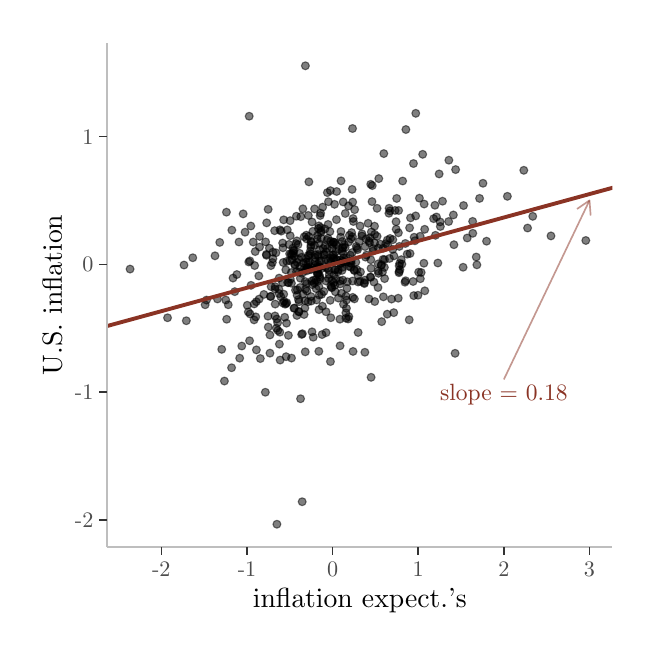
\begin{tikzpicture}[x=1pt,y=1pt]
\definecolor{fillColor}{RGB}{255,255,255}
\path[use as bounding box,fill=fillColor,fill opacity=0.00] (0,0) rectangle (216.81,216.81);
\begin{scope}
\path[clip] (  0.00,  0.00) rectangle (216.81,216.81);
\definecolor{drawColor}{RGB}{255,255,255}
\definecolor{fillColor}{RGB}{255,255,255}

\path[draw=drawColor,line width= 0.6pt,line join=round,line cap=round,fill=fillColor] (  0.00,  0.00) rectangle (216.81,216.81);
\end{scope}
\begin{scope}
\path[clip] ( 28.70, 29.10) rectangle (211.31,211.31);
\definecolor{drawColor}{RGB}{255,255,255}

\path[draw=drawColor,line width= 0.6pt,line join=round] ( 28.70, 38.89) --
	(211.31, 38.89);

\path[draw=drawColor,line width= 0.6pt,line join=round] ( 28.70, 85.08) --
	(211.31, 85.08);

\path[draw=drawColor,line width= 0.6pt,line join=round] ( 28.70,131.28) --
	(211.31,131.28);

\path[draw=drawColor,line width= 0.6pt,line join=round] ( 28.70,177.48) --
	(211.31,177.48);

\path[draw=drawColor,line width= 0.6pt,line join=round] ( 48.30, 29.10) --
	( 48.30,211.31);

\path[draw=drawColor,line width= 0.6pt,line join=round] ( 79.25, 29.10) --
	( 79.25,211.31);

\path[draw=drawColor,line width= 0.6pt,line join=round] (110.19, 29.10) --
	(110.19,211.31);

\path[draw=drawColor,line width= 0.6pt,line join=round] (141.13, 29.10) --
	(141.13,211.31);

\path[draw=drawColor,line width= 0.6pt,line join=round] (172.07, 29.10) --
	(172.07,211.31);

\path[draw=drawColor,line width= 0.6pt,line join=round] (203.01, 29.10) --
	(203.01,211.31);
\definecolor{drawColor}{RGB}{0,0,0}
\definecolor{fillColor}{RGB}{0,0,0}

\path[draw=drawColor,draw opacity=0.50,line width= 0.4pt,line join=round,line cap=round,fill=fillColor,fill opacity=0.50] (164.52,160.58) circle (  1.43);

\path[draw=drawColor,draw opacity=0.50,line width= 0.4pt,line join=round,line cap=round,fill=fillColor,fill opacity=0.50] (148.22,131.77) circle (  1.43);

\path[draw=drawColor,draw opacity=0.50,line width= 0.4pt,line join=round,line cap=round,fill=fillColor,fill opacity=0.50] (138.01,144.47) circle (  1.43);

\path[draw=drawColor,draw opacity=0.50,line width= 0.4pt,line join=round,line cap=round,fill=fillColor,fill opacity=0.50] (162.09,133.94) circle (  1.43);

\path[draw=drawColor,draw opacity=0.50,line width= 0.4pt,line join=round,line cap=round,fill=fillColor,fill opacity=0.50] (135.50,161.40) circle (  1.43);

\path[draw=drawColor,draw opacity=0.50,line width= 0.4pt,line join=round,line cap=round,fill=fillColor,fill opacity=0.50] (123.34,139.71) circle (  1.43);

\path[draw=drawColor,draw opacity=0.50,line width= 0.4pt,line join=round,line cap=round,fill=fillColor,fill opacity=0.50] (139.27,125.09) circle (  1.43);

\path[draw=drawColor,draw opacity=0.50,line width= 0.4pt,line join=round,line cap=round,fill=fillColor,fill opacity=0.50] (143.46,143.95) circle (  1.43);

\path[draw=drawColor,draw opacity=0.50,line width= 0.4pt,line join=round,line cap=round,fill=fillColor,fill opacity=0.50] (160.84,142.51) circle (  1.43);

\path[draw=drawColor,draw opacity=0.50,line width= 0.4pt,line join=round,line cap=round,fill=fillColor,fill opacity=0.50] (173.34,155.87) circle (  1.43);

\path[draw=drawColor,draw opacity=0.50,line width= 0.4pt,line join=round,line cap=round,fill=fillColor,fill opacity=0.50] (158.83,140.81) circle (  1.43);

\path[draw=drawColor,draw opacity=0.50,line width= 0.4pt,line join=round,line cap=round,fill=fillColor,fill opacity=0.50] (165.81,139.65) circle (  1.43);

\path[draw=drawColor,draw opacity=0.50,line width= 0.4pt,line join=round,line cap=round,fill=fillColor,fill opacity=0.50] (189.09,141.56) circle (  1.43);

\path[draw=drawColor,draw opacity=0.50,line width= 0.4pt,line join=round,line cap=round,fill=fillColor,fill opacity=0.50] (182.51,148.64) circle (  1.43);

\path[draw=drawColor,draw opacity=0.50,line width= 0.4pt,line join=round,line cap=round,fill=fillColor,fill opacity=0.50] (180.64,144.41) circle (  1.43);

\path[draw=drawColor,draw opacity=0.50,line width= 0.4pt,line join=round,line cap=round,fill=fillColor,fill opacity=0.50] (160.79,146.81) circle (  1.43);

\path[draw=drawColor,draw opacity=0.50,line width= 0.4pt,line join=round,line cap=round,fill=fillColor,fill opacity=0.50] (134.24,130.73) circle (  1.43);

\path[draw=drawColor,draw opacity=0.50,line width= 0.4pt,line join=round,line cap=round,fill=fillColor,fill opacity=0.50] (123.02,146.12) circle (  1.43);

\path[draw=drawColor,draw opacity=0.50,line width= 0.4pt,line join=round,line cap=round,fill=fillColor,fill opacity=0.50] (163.29,155.12) circle (  1.43);

\path[draw=drawColor,draw opacity=0.50,line width= 0.4pt,line join=round,line cap=round,fill=fillColor,fill opacity=0.50] (141.56,155.20) circle (  1.43);

\path[draw=drawColor,draw opacity=0.50,line width= 0.4pt,line join=round,line cap=round,fill=fillColor,fill opacity=0.50] (157.50,152.54) circle (  1.43);

\path[draw=drawColor,draw opacity=0.50,line width= 0.4pt,line join=round,line cap=round,fill=fillColor,fill opacity=0.50] (131.96,140.20) circle (  1.43);

\path[draw=drawColor,draw opacity=0.50,line width= 0.4pt,line join=round,line cap=round,fill=fillColor,fill opacity=0.50] (149.91,154.10) circle (  1.43);

\path[draw=drawColor,draw opacity=0.50,line width= 0.4pt,line join=round,line cap=round,fill=fillColor,fill opacity=0.50] (100.80,128.92) circle (  1.43);

\path[draw=drawColor,draw opacity=0.50,line width= 0.4pt,line join=round,line cap=round,fill=fillColor,fill opacity=0.50] ( 59.66,133.67) circle (  1.43);

\path[draw=drawColor,draw opacity=0.50,line width= 0.4pt,line join=round,line cap=round,fill=fillColor,fill opacity=0.50] ( 67.69,134.37) circle (  1.43);

\path[draw=drawColor,draw opacity=0.50,line width= 0.4pt,line join=round,line cap=round,fill=fillColor,fill opacity=0.50] ( 71.09, 89.12) circle (  1.43);

\path[draw=drawColor,draw opacity=0.50,line width= 0.4pt,line join=round,line cap=round,fill=fillColor,fill opacity=0.50] ( 99.44,151.36) circle (  1.43);

\path[draw=drawColor,draw opacity=0.50,line width= 0.4pt,line join=round,line cap=round,fill=fillColor,fill opacity=0.50] (111.19,129.32) circle (  1.43);

\path[draw=drawColor,draw opacity=0.50,line width= 0.4pt,line join=round,line cap=round,fill=fillColor,fill opacity=0.50] (118.58,132.08) circle (  1.43);

\path[draw=drawColor,draw opacity=0.50,line width= 0.4pt,line join=round,line cap=round,fill=fillColor,fill opacity=0.50] ( 81.51,139.34) circle (  1.43);

\path[draw=drawColor,draw opacity=0.50,line width= 0.4pt,line join=round,line cap=round,fill=fillColor,fill opacity=0.50] (126.59,122.92) circle (  1.43);

\path[draw=drawColor,draw opacity=0.50,line width= 0.4pt,line join=round,line cap=round,fill=fillColor,fill opacity=0.50] (101.35,117.78) circle (  1.43);

\path[draw=drawColor,draw opacity=0.50,line width= 0.4pt,line join=round,line cap=round,fill=fillColor,fill opacity=0.50] (112.21,129.33) circle (  1.43);

\path[draw=drawColor,draw opacity=0.50,line width= 0.4pt,line join=round,line cap=round,fill=fillColor,fill opacity=0.50] ( 87.54,105.77) circle (  1.43);

\path[draw=drawColor,draw opacity=0.50,line width= 0.4pt,line join=round,line cap=round,fill=fillColor,fill opacity=0.50] (124.07,129.85) circle (  1.43);

\path[draw=drawColor,draw opacity=0.50,line width= 0.4pt,line join=round,line cap=round,fill=fillColor,fill opacity=0.50] (109.92,125.48) circle (  1.43);

\path[draw=drawColor,draw opacity=0.50,line width= 0.4pt,line join=round,line cap=round,fill=fillColor,fill opacity=0.50] (102.13,136.07) circle (  1.43);

\path[draw=drawColor,draw opacity=0.50,line width= 0.4pt,line join=round,line cap=round,fill=fillColor,fill opacity=0.50] ( 80.05,184.81) circle (  1.43);

\path[draw=drawColor,draw opacity=0.50,line width= 0.4pt,line join=round,line cap=round,fill=fillColor,fill opacity=0.50] ( 57.32,110.91) circle (  1.43);

\path[draw=drawColor,draw opacity=0.50,line width= 0.4pt,line join=round,line cap=round,fill=fillColor,fill opacity=0.50] ( 71.82,150.14) circle (  1.43);

\path[draw=drawColor,draw opacity=0.50,line width= 0.4pt,line join=round,line cap=round,fill=fillColor,fill opacity=0.50] ( 70.12,100.58) circle (  1.43);

\path[draw=drawColor,draw opacity=0.50,line width= 0.4pt,line join=round,line cap=round,fill=fillColor,fill opacity=0.50] (100.38,122.31) circle (  1.43);

\path[draw=drawColor,draw opacity=0.50,line width= 0.4pt,line join=round,line cap=round,fill=fillColor,fill opacity=0.50] ( 64.13,116.68) circle (  1.43);

\path[draw=drawColor,draw opacity=0.50,line width= 0.4pt,line join=round,line cap=round,fill=fillColor,fill opacity=0.50] ( 72.48,116.68) circle (  1.43);

\path[draw=drawColor,draw opacity=0.50,line width= 0.4pt,line join=round,line cap=round,fill=fillColor,fill opacity=0.50] ( 81.86,116.98) circle (  1.43);

\path[draw=drawColor,draw opacity=0.50,line width= 0.4pt,line join=round,line cap=round,fill=fillColor,fill opacity=0.50] ( 86.84,112.55) circle (  1.43);

\path[draw=drawColor,draw opacity=0.50,line width= 0.4pt,line join=round,line cap=round,fill=fillColor,fill opacity=0.50] ( 96.02,136.06) circle (  1.43);

\path[draw=drawColor,draw opacity=0.50,line width= 0.4pt,line join=round,line cap=round,fill=fillColor,fill opacity=0.50] ( 77.87,149.52) circle (  1.43);

\path[draw=drawColor,draw opacity=0.50,line width= 0.4pt,line join=round,line cap=round,fill=fillColor,fill opacity=0.50] ( 92.14,138.98) circle (  1.43);

\path[draw=drawColor,draw opacity=0.50,line width= 0.4pt,line join=round,line cap=round,fill=fillColor,fill opacity=0.50] ( 90.96,102.46) circle (  1.43);

\path[draw=drawColor,draw opacity=0.50,line width= 0.4pt,line join=round,line cap=round,fill=fillColor,fill opacity=0.50] (120.09,125.16) circle (  1.43);

\path[draw=drawColor,draw opacity=0.50,line width= 0.4pt,line join=round,line cap=round,fill=fillColor,fill opacity=0.50] ( 95.34, 97.42) circle (  1.43);

\path[draw=drawColor,draw opacity=0.50,line width= 0.4pt,line join=round,line cap=round,fill=fillColor,fill opacity=0.50] (124.52,159.75) circle (  1.43);

\path[draw=drawColor,draw opacity=0.50,line width= 0.4pt,line join=round,line cap=round,fill=fillColor,fill opacity=0.50] (100.30, 99.67) circle (  1.43);

\path[draw=drawColor,draw opacity=0.50,line width= 0.4pt,line join=round,line cap=round,fill=fillColor,fill opacity=0.50] (117.47,119.36) circle (  1.43);

\path[draw=drawColor,draw opacity=0.50,line width= 0.4pt,line join=round,line cap=round,fill=fillColor,fill opacity=0.50] (104.59,140.43) circle (  1.43);

\path[draw=drawColor,draw opacity=0.50,line width= 0.4pt,line join=round,line cap=round,fill=fillColor,fill opacity=0.50] ( 96.78,121.97) circle (  1.43);

\path[draw=drawColor,draw opacity=0.50,line width= 0.4pt,line join=round,line cap=round,fill=fillColor,fill opacity=0.50] ( 73.78,143.65) circle (  1.43);

\path[draw=drawColor,draw opacity=0.50,line width= 0.4pt,line join=round,line cap=round,fill=fillColor,fill opacity=0.50] ( 97.10,148.67) circle (  1.43);

\path[draw=drawColor,draw opacity=0.50,line width= 0.4pt,line join=round,line cap=round,fill=fillColor,fill opacity=0.50] ( 87.55, 99.20) circle (  1.43);

\path[draw=drawColor,draw opacity=0.50,line width= 0.4pt,line join=round,line cap=round,fill=fillColor,fill opacity=0.50] (106.38,105.92) circle (  1.43);

\path[draw=drawColor,draw opacity=0.50,line width= 0.4pt,line join=round,line cap=round,fill=fillColor,fill opacity=0.50] (133.11,146.70) circle (  1.43);

\path[draw=drawColor,draw opacity=0.50,line width= 0.4pt,line join=round,line cap=round,fill=fillColor,fill opacity=0.50] (135.00,132.97) circle (  1.43);

\path[draw=drawColor,draw opacity=0.50,line width= 0.4pt,line join=round,line cap=round,fill=fillColor,fill opacity=0.50] (133.16,143.97) circle (  1.43);

\path[draw=drawColor,draw opacity=0.50,line width= 0.4pt,line join=round,line cap=round,fill=fillColor,fill opacity=0.50] (136.56,125.36) circle (  1.43);

\path[draw=drawColor,draw opacity=0.50,line width= 0.4pt,line join=round,line cap=round,fill=fillColor,fill opacity=0.50] (124.43,153.96) circle (  1.43);

\path[draw=drawColor,draw opacity=0.50,line width= 0.4pt,line join=round,line cap=round,fill=fillColor,fill opacity=0.50] (118.15,151.05) circle (  1.43);

\path[draw=drawColor,draw opacity=0.50,line width= 0.4pt,line join=round,line cap=round,fill=fillColor,fill opacity=0.50] ( 91.16,143.75) circle (  1.43);

\path[draw=drawColor,draw opacity=0.50,line width= 0.4pt,line join=round,line cap=round,fill=fillColor,fill opacity=0.50] ( 93.81,143.73) circle (  1.43);

\path[draw=drawColor,draw opacity=0.50,line width= 0.4pt,line join=round,line cap=round,fill=fillColor,fill opacity=0.50] ( 82.22,135.90) circle (  1.43);

\path[draw=drawColor,draw opacity=0.50,line width= 0.4pt,line join=round,line cap=round,fill=fillColor,fill opacity=0.50] (115.19,115.39) circle (  1.43);

\path[draw=drawColor,draw opacity=0.50,line width= 0.4pt,line join=round,line cap=round,fill=fillColor,fill opacity=0.50] (115.00,132.06) circle (  1.43);

\path[draw=drawColor,draw opacity=0.50,line width= 0.4pt,line join=round,line cap=round,fill=fillColor,fill opacity=0.50] (116.57,134.64) circle (  1.43);

\path[draw=drawColor,draw opacity=0.50,line width= 0.4pt,line join=round,line cap=round,fill=fillColor,fill opacity=0.50] (102.26,130.38) circle (  1.43);

\path[draw=drawColor,draw opacity=0.50,line width= 0.4pt,line join=round,line cap=round,fill=fillColor,fill opacity=0.50] ( 93.62,132.36) circle (  1.43);

\path[draw=drawColor,draw opacity=0.50,line width= 0.4pt,line join=round,line cap=round,fill=fillColor,fill opacity=0.50] ( 92.33,131.97) circle (  1.43);

\path[draw=drawColor,draw opacity=0.50,line width= 0.4pt,line join=round,line cap=round,fill=fillColor,fill opacity=0.50] (113.04,131.88) circle (  1.43);

\path[draw=drawColor,draw opacity=0.50,line width= 0.4pt,line join=round,line cap=round,fill=fillColor,fill opacity=0.50] (110.66,127.46) circle (  1.43);

\path[draw=drawColor,draw opacity=0.50,line width= 0.4pt,line join=round,line cap=round,fill=fillColor,fill opacity=0.50] (108.29,129.78) circle (  1.43);

\path[draw=drawColor,draw opacity=0.50,line width= 0.4pt,line join=round,line cap=round,fill=fillColor,fill opacity=0.50] ( 90.33,110.20) circle (  1.43);

\path[draw=drawColor,draw opacity=0.50,line width= 0.4pt,line join=round,line cap=round,fill=fillColor,fill opacity=0.50] (111.58,147.44) circle (  1.43);

\path[draw=drawColor,draw opacity=0.50,line width= 0.4pt,line join=round,line cap=round,fill=fillColor,fill opacity=0.50] (101.82,134.55) circle (  1.43);

\path[draw=drawColor,draw opacity=0.50,line width= 0.4pt,line join=round,line cap=round,fill=fillColor,fill opacity=0.50] (118.05,118.80) circle (  1.43);

\path[draw=drawColor,draw opacity=0.50,line width= 0.4pt,line join=round,line cap=round,fill=fillColor,fill opacity=0.50] (107.47,138.08) circle (  1.43);

\path[draw=drawColor,draw opacity=0.50,line width= 0.4pt,line join=round,line cap=round,fill=fillColor,fill opacity=0.50] (110.54,134.71) circle (  1.43);

\path[draw=drawColor,draw opacity=0.50,line width= 0.4pt,line join=round,line cap=round,fill=fillColor,fill opacity=0.50] ( 85.36,120.42) circle (  1.43);

\path[draw=drawColor,draw opacity=0.50,line width= 0.4pt,line join=round,line cap=round,fill=fillColor,fill opacity=0.50] ( 94.73,132.64) circle (  1.43);

\path[draw=drawColor,draw opacity=0.50,line width= 0.4pt,line join=round,line cap=round,fill=fillColor,fill opacity=0.50] (104.65,127.86) circle (  1.43);

\path[draw=drawColor,draw opacity=0.50,line width= 0.4pt,line join=round,line cap=round,fill=fillColor,fill opacity=0.50] (123.98,132.95) circle (  1.43);

\path[draw=drawColor,draw opacity=0.50,line width= 0.4pt,line join=round,line cap=round,fill=fillColor,fill opacity=0.50] (107.43,144.03) circle (  1.43);

\path[draw=drawColor,draw opacity=0.50,line width= 0.4pt,line join=round,line cap=round,fill=fillColor,fill opacity=0.50] (121.92,137.73) circle (  1.43);

\path[draw=drawColor,draw opacity=0.50,line width= 0.4pt,line join=round,line cap=round,fill=fillColor,fill opacity=0.50] ( 89.72,135.47) circle (  1.43);

\path[draw=drawColor,draw opacity=0.50,line width= 0.4pt,line join=round,line cap=round,fill=fillColor,fill opacity=0.50] ( 73.68, 93.92) circle (  1.43);

\path[draw=drawColor,draw opacity=0.50,line width= 0.4pt,line join=round,line cap=round,fill=fillColor,fill opacity=0.50] ( 80.18,103.68) circle (  1.43);

\path[draw=drawColor,draw opacity=0.50,line width= 0.4pt,line join=round,line cap=round,fill=fillColor,fill opacity=0.50] (103.57,124.53) circle (  1.43);

\path[draw=drawColor,draw opacity=0.50,line width= 0.4pt,line join=round,line cap=round,fill=fillColor,fill opacity=0.50] (113.10,141.11) circle (  1.43);

\path[draw=drawColor,draw opacity=0.50,line width= 0.4pt,line join=round,line cap=round,fill=fillColor,fill opacity=0.50] (126.65,128.85) circle (  1.43);

\path[draw=drawColor,draw opacity=0.50,line width= 0.4pt,line join=round,line cap=round,fill=fillColor,fill opacity=0.50] (104.72,125.14) circle (  1.43);

\path[draw=drawColor,draw opacity=0.50,line width= 0.4pt,line join=round,line cap=round,fill=fillColor,fill opacity=0.50] (117.95,129.29) circle (  1.43);

\path[draw=drawColor,draw opacity=0.50,line width= 0.4pt,line join=round,line cap=round,fill=fillColor,fill opacity=0.50] (108.52,140.72) circle (  1.43);

\path[draw=drawColor,draw opacity=0.50,line width= 0.4pt,line join=round,line cap=round,fill=fillColor,fill opacity=0.50] (114.12,116.87) circle (  1.43);

\path[draw=drawColor,draw opacity=0.50,line width= 0.4pt,line join=round,line cap=round,fill=fillColor,fill opacity=0.50] (110.99,123.71) circle (  1.43);

\path[draw=drawColor,draw opacity=0.50,line width= 0.4pt,line join=round,line cap=round,fill=fillColor,fill opacity=0.50] (127.82,131.19) circle (  1.43);

\path[draw=drawColor,draw opacity=0.50,line width= 0.4pt,line join=round,line cap=round,fill=fillColor,fill opacity=0.50] (129.38,138.74) circle (  1.43);

\path[draw=drawColor,draw opacity=0.50,line width= 0.4pt,line join=round,line cap=round,fill=fillColor,fill opacity=0.50] (134.04,150.75) circle (  1.43);

\path[draw=drawColor,draw opacity=0.50,line width= 0.4pt,line join=round,line cap=round,fill=fillColor,fill opacity=0.50] (113.23,161.46) circle (  1.43);

\path[draw=drawColor,draw opacity=0.50,line width= 0.4pt,line join=round,line cap=round,fill=fillColor,fill opacity=0.50] ( 86.89,151.17) circle (  1.43);

\path[draw=drawColor,draw opacity=0.50,line width= 0.4pt,line join=round,line cap=round,fill=fillColor,fill opacity=0.50] ( 92.18,117.34) circle (  1.43);

\path[draw=drawColor,draw opacity=0.50,line width= 0.4pt,line join=round,line cap=round,fill=fillColor,fill opacity=0.50] ( 99.92,141.24) circle (  1.43);

\path[draw=drawColor,draw opacity=0.50,line width= 0.4pt,line join=round,line cap=round,fill=fillColor,fill opacity=0.50] ( 92.26,137.27) circle (  1.43);

\path[draw=drawColor,draw opacity=0.50,line width= 0.4pt,line join=round,line cap=round,fill=fillColor,fill opacity=0.50] (105.03,144.22) circle (  1.43);

\path[draw=drawColor,draw opacity=0.50,line width= 0.4pt,line join=round,line cap=round,fill=fillColor,fill opacity=0.50] ( 87.98,123.22) circle (  1.43);

\path[draw=drawColor,draw opacity=0.50,line width= 0.4pt,line join=round,line cap=round,fill=fillColor,fill opacity=0.50] ( 97.69,138.40) circle (  1.43);

\path[draw=drawColor,draw opacity=0.50,line width= 0.4pt,line join=round,line cap=round,fill=fillColor,fill opacity=0.50] ( 87.34,137.12) circle (  1.43);

\path[draw=drawColor,draw opacity=0.50,line width= 0.4pt,line join=round,line cap=round,fill=fillColor,fill opacity=0.50] ( 83.63,118.73) circle (  1.43);

\path[draw=drawColor,draw opacity=0.50,line width= 0.4pt,line join=round,line cap=round,fill=fillColor,fill opacity=0.50] ( 99.13,128.04) circle (  1.43);

\path[draw=drawColor,draw opacity=0.50,line width= 0.4pt,line join=round,line cap=round,fill=fillColor,fill opacity=0.50] (104.09,125.63) circle (  1.43);

\path[draw=drawColor,draw opacity=0.50,line width= 0.4pt,line join=round,line cap=round,fill=fillColor,fill opacity=0.50] (104.04,129.58) circle (  1.43);

\path[draw=drawColor,draw opacity=0.50,line width= 0.4pt,line join=round,line cap=round,fill=fillColor,fill opacity=0.50] (115.99,139.36) circle (  1.43);

\path[draw=drawColor,draw opacity=0.50,line width= 0.4pt,line join=round,line cap=round,fill=fillColor,fill opacity=0.50] (111.41,125.93) circle (  1.43);

\path[draw=drawColor,draw opacity=0.50,line width= 0.4pt,line join=round,line cap=round,fill=fillColor,fill opacity=0.50] (116.88,131.63) circle (  1.43);

\path[draw=drawColor,draw opacity=0.50,line width= 0.4pt,line join=round,line cap=round,fill=fillColor,fill opacity=0.50] (136.47,138.83) circle (  1.43);

\path[draw=drawColor,draw opacity=0.50,line width= 0.4pt,line join=round,line cap=round,fill=fillColor,fill opacity=0.50] (128.98,126.13) circle (  1.43);

\path[draw=drawColor,draw opacity=0.50,line width= 0.4pt,line join=round,line cap=round,fill=fillColor,fill opacity=0.50] (124.72,136.07) circle (  1.43);

\path[draw=drawColor,draw opacity=0.50,line width= 0.4pt,line join=round,line cap=round,fill=fillColor,fill opacity=0.50] (116.91,132.56) circle (  1.43);

\path[draw=drawColor,draw opacity=0.50,line width= 0.4pt,line join=round,line cap=round,fill=fillColor,fill opacity=0.50] (118.06,129.02) circle (  1.43);

\path[draw=drawColor,draw opacity=0.50,line width= 0.4pt,line join=round,line cap=round,fill=fillColor,fill opacity=0.50] (119.83,139.56) circle (  1.43);

\path[draw=drawColor,draw opacity=0.50,line width= 0.4pt,line join=round,line cap=round,fill=fillColor,fill opacity=0.50] (113.79,130.24) circle (  1.43);

\path[draw=drawColor,draw opacity=0.50,line width= 0.4pt,line join=round,line cap=round,fill=fillColor,fill opacity=0.50] (103.63,138.18) circle (  1.43);

\path[draw=drawColor,draw opacity=0.50,line width= 0.4pt,line join=round,line cap=round,fill=fillColor,fill opacity=0.50] (105.33,138.81) circle (  1.43);

\path[draw=drawColor,draw opacity=0.50,line width= 0.4pt,line join=round,line cap=round,fill=fillColor,fill opacity=0.50] (111.69,133.03) circle (  1.43);

\path[draw=drawColor,draw opacity=0.50,line width= 0.4pt,line join=round,line cap=round,fill=fillColor,fill opacity=0.50] (123.67,140.91) circle (  1.43);

\path[draw=drawColor,draw opacity=0.50,line width= 0.4pt,line join=round,line cap=round,fill=fillColor,fill opacity=0.50] (100.92,121.66) circle (  1.43);

\path[draw=drawColor,draw opacity=0.50,line width= 0.4pt,line join=round,line cap=round,fill=fillColor,fill opacity=0.50] (103.83,130.93) circle (  1.43);

\path[draw=drawColor,draw opacity=0.50,line width= 0.4pt,line join=round,line cap=round,fill=fillColor,fill opacity=0.50] ( 89.37,112.64) circle (  1.43);

\path[draw=drawColor,draw opacity=0.50,line width= 0.4pt,line join=round,line cap=round,fill=fillColor,fill opacity=0.50] (106.00,132.57) circle (  1.43);

\path[draw=drawColor,draw opacity=0.50,line width= 0.4pt,line join=round,line cap=round,fill=fillColor,fill opacity=0.50] (110.43,139.32) circle (  1.43);

\path[draw=drawColor,draw opacity=0.50,line width= 0.4pt,line join=round,line cap=round,fill=fillColor,fill opacity=0.50] (110.98,129.39) circle (  1.43);

\path[draw=drawColor,draw opacity=0.50,line width= 0.4pt,line join=round,line cap=round,fill=fillColor,fill opacity=0.50] (101.08,130.14) circle (  1.43);

\path[draw=drawColor,draw opacity=0.50,line width= 0.4pt,line join=round,line cap=round,fill=fillColor,fill opacity=0.50] (109.37,157.91) circle (  1.43);

\path[draw=drawColor,draw opacity=0.50,line width= 0.4pt,line join=round,line cap=round,fill=fillColor,fill opacity=0.50] ( 90.88,120.72) circle (  1.43);

\path[draw=drawColor,draw opacity=0.50,line width= 0.4pt,line join=round,line cap=round,fill=fillColor,fill opacity=0.50] ( 95.53,132.96) circle (  1.43);

\path[draw=drawColor,draw opacity=0.50,line width= 0.4pt,line join=round,line cap=round,fill=fillColor,fill opacity=0.50] ( 89.86,108.22) circle (  1.43);

\path[draw=drawColor,draw opacity=0.50,line width= 0.4pt,line join=round,line cap=round,fill=fillColor,fill opacity=0.50] (104.85,127.92) circle (  1.43);

\path[draw=drawColor,draw opacity=0.50,line width= 0.4pt,line join=round,line cap=round,fill=fillColor,fill opacity=0.50] (114.76,149.66) circle (  1.43);

\path[draw=drawColor,draw opacity=0.50,line width= 0.4pt,line join=round,line cap=round,fill=fillColor,fill opacity=0.50] (104.83,128.09) circle (  1.43);

\path[draw=drawColor,draw opacity=0.50,line width= 0.4pt,line join=round,line cap=round,fill=fillColor,fill opacity=0.50] (128.69,171.31) circle (  1.43);

\path[draw=drawColor,draw opacity=0.50,line width= 0.4pt,line join=round,line cap=round,fill=fillColor,fill opacity=0.50] ( 97.79,133.18) circle (  1.43);

\path[draw=drawColor,draw opacity=0.50,line width= 0.4pt,line join=round,line cap=round,fill=fillColor,fill opacity=0.50] (114.73,137.42) circle (  1.43);

\path[draw=drawColor,draw opacity=0.50,line width= 0.4pt,line join=round,line cap=round,fill=fillColor,fill opacity=0.50] ( 89.37,122.36) circle (  1.43);

\path[draw=drawColor,draw opacity=0.50,line width= 0.4pt,line join=round,line cap=round,fill=fillColor,fill opacity=0.50] ( 83.80,141.39) circle (  1.43);

\path[draw=drawColor,draw opacity=0.50,line width= 0.4pt,line join=round,line cap=round,fill=fillColor,fill opacity=0.50] ( 77.36,101.77) circle (  1.43);

\path[draw=drawColor,draw opacity=0.50,line width= 0.4pt,line join=round,line cap=round,fill=fillColor,fill opacity=0.50] ( 80.29,132.53) circle (  1.43);

\path[draw=drawColor,draw opacity=0.50,line width= 0.4pt,line join=round,line cap=round,fill=fillColor,fill opacity=0.50] ( 80.37,113.36) circle (  1.43);

\path[draw=drawColor,draw opacity=0.50,line width= 0.4pt,line join=round,line cap=round,fill=fillColor,fill opacity=0.50] (101.54,141.38) circle (  1.43);

\path[draw=drawColor,draw opacity=0.50,line width= 0.4pt,line join=round,line cap=round,fill=fillColor,fill opacity=0.50] ( 85.97,139.40) circle (  1.43);

\path[draw=drawColor,draw opacity=0.50,line width= 0.4pt,line join=round,line cap=round,fill=fillColor,fill opacity=0.50] ( 71.91,111.44) circle (  1.43);

\path[draw=drawColor,draw opacity=0.50,line width= 0.4pt,line join=round,line cap=round,fill=fillColor,fill opacity=0.50] ( 83.53,127.10) circle (  1.43);

\path[draw=drawColor,draw opacity=0.50,line width= 0.4pt,line join=round,line cap=round,fill=fillColor,fill opacity=0.50] ( 81.81,111.22) circle (  1.43);

\path[draw=drawColor,draw opacity=0.50,line width= 0.4pt,line join=round,line cap=round,fill=fillColor,fill opacity=0.50] ( 92.13,124.71) circle (  1.43);

\path[draw=drawColor,draw opacity=0.50,line width= 0.4pt,line join=round,line cap=round,fill=fillColor,fill opacity=0.50] (109.54,112.00) circle (  1.43);

\path[draw=drawColor,draw opacity=0.50,line width= 0.4pt,line join=round,line cap=round,fill=fillColor,fill opacity=0.50] (106.60,151.97) circle (  1.43);

\path[draw=drawColor,draw opacity=0.50,line width= 0.4pt,line join=round,line cap=round,fill=fillColor,fill opacity=0.50] ( 64.63,118.38) circle (  1.43);

\path[draw=drawColor,draw opacity=0.50,line width= 0.4pt,line join=round,line cap=round,fill=fillColor,fill opacity=0.50] ( 74.84,121.42) circle (  1.43);

\path[draw=drawColor,draw opacity=0.50,line width= 0.4pt,line join=round,line cap=round,fill=fillColor,fill opacity=0.50] ( 80.63,145.14) circle (  1.43);

\path[draw=drawColor,draw opacity=0.50,line width= 0.4pt,line join=round,line cap=round,fill=fillColor,fill opacity=0.50] ( 78.55,142.90) circle (  1.43);

\path[draw=drawColor,draw opacity=0.50,line width= 0.4pt,line join=round,line cap=round,fill=fillColor,fill opacity=0.50] ( 80.71,123.71) circle (  1.43);

\path[draw=drawColor,draw opacity=0.50,line width= 0.4pt,line join=round,line cap=round,fill=fillColor,fill opacity=0.50] ( 75.59,127.60) circle (  1.43);

\path[draw=drawColor,draw opacity=0.50,line width= 0.4pt,line join=round,line cap=round,fill=fillColor,fill opacity=0.50] ( 95.92,135.34) circle (  1.43);

\path[draw=drawColor,draw opacity=0.50,line width= 0.4pt,line join=round,line cap=round,fill=fillColor,fill opacity=0.50] ( 83.80,137.55) circle (  1.43);

\path[draw=drawColor,draw opacity=0.50,line width= 0.4pt,line join=round,line cap=round,fill=fillColor,fill opacity=0.50] ( 94.29,124.69) circle (  1.43);

\path[draw=drawColor,draw opacity=0.50,line width= 0.4pt,line join=round,line cap=round,fill=fillColor,fill opacity=0.50] ( 96.51,131.26) circle (  1.43);

\path[draw=drawColor,draw opacity=0.50,line width= 0.4pt,line join=round,line cap=round,fill=fillColor,fill opacity=0.50] ( 86.36,146.28) circle (  1.43);

\path[draw=drawColor,draw opacity=0.50,line width= 0.4pt,line join=round,line cap=round,fill=fillColor,fill opacity=0.50] ( 89.44,116.93) circle (  1.43);

\path[draw=drawColor,draw opacity=0.50,line width= 0.4pt,line join=round,line cap=round,fill=fillColor,fill opacity=0.50] ( 82.03,130.85) circle (  1.43);

\path[draw=drawColor,draw opacity=0.50,line width= 0.4pt,line join=round,line cap=round,fill=fillColor,fill opacity=0.50] ( 92.50,147.37) circle (  1.43);

\path[draw=drawColor,draw opacity=0.50,line width= 0.4pt,line join=round,line cap=round,fill=fillColor,fill opacity=0.50] ( 89.43,123.23) circle (  1.43);

\path[draw=drawColor,draw opacity=0.50,line width= 0.4pt,line join=round,line cap=round,fill=fillColor,fill opacity=0.50] (109.53,123.55) circle (  1.43);

\path[draw=drawColor,draw opacity=0.50,line width= 0.4pt,line join=round,line cap=round,fill=fillColor,fill opacity=0.50] ( 91.60,143.29) circle (  1.43);

\path[draw=drawColor,draw opacity=0.50,line width= 0.4pt,line join=round,line cap=round,fill=fillColor,fill opacity=0.50] (101.91,129.55) circle (  1.43);

\path[draw=drawColor,draw opacity=0.50,line width= 0.4pt,line join=round,line cap=round,fill=fillColor,fill opacity=0.50] (113.36,120.84) circle (  1.43);

\path[draw=drawColor,draw opacity=0.50,line width= 0.4pt,line join=round,line cap=round,fill=fillColor,fill opacity=0.50] (107.65,130.35) circle (  1.43);

\path[draw=drawColor,draw opacity=0.50,line width= 0.4pt,line join=round,line cap=round,fill=fillColor,fill opacity=0.50] (111.42,132.94) circle (  1.43);

\path[draw=drawColor,draw opacity=0.50,line width= 0.4pt,line join=round,line cap=round,fill=fillColor,fill opacity=0.50] (105.52,126.72) circle (  1.43);

\path[draw=drawColor,draw opacity=0.50,line width= 0.4pt,line join=round,line cap=round,fill=fillColor,fill opacity=0.50] (108.66,132.57) circle (  1.43);

\path[draw=drawColor,draw opacity=0.50,line width= 0.4pt,line join=round,line cap=round,fill=fillColor,fill opacity=0.50] ( 98.37,130.43) circle (  1.43);

\path[draw=drawColor,draw opacity=0.50,line width= 0.4pt,line join=round,line cap=round,fill=fillColor,fill opacity=0.50] ( 96.31,134.21) circle (  1.43);

\path[draw=drawColor,draw opacity=0.50,line width= 0.4pt,line join=round,line cap=round,fill=fillColor,fill opacity=0.50] ( 97.30,112.81) circle (  1.43);

\path[draw=drawColor,draw opacity=0.50,line width= 0.4pt,line join=round,line cap=round,fill=fillColor,fill opacity=0.50] (103.07,143.22) circle (  1.43);

\path[draw=drawColor,draw opacity=0.50,line width= 0.4pt,line join=round,line cap=round,fill=fillColor,fill opacity=0.50] (112.97,132.81) circle (  1.43);

\path[draw=drawColor,draw opacity=0.50,line width= 0.4pt,line join=round,line cap=round,fill=fillColor,fill opacity=0.50] (105.28,114.92) circle (  1.43);

\path[draw=drawColor,draw opacity=0.50,line width= 0.4pt,line join=round,line cap=round,fill=fillColor,fill opacity=0.50] (114.12,135.07) circle (  1.43);

\path[draw=drawColor,draw opacity=0.50,line width= 0.4pt,line join=round,line cap=round,fill=fillColor,fill opacity=0.50] (102.44,139.63) circle (  1.43);

\path[draw=drawColor,draw opacity=0.50,line width= 0.4pt,line join=round,line cap=round,fill=fillColor,fill opacity=0.50] (101.34,134.52) circle (  1.43);

\path[draw=drawColor,draw opacity=0.50,line width= 0.4pt,line join=round,line cap=round,fill=fillColor,fill opacity=0.50] (119.21,136.59) circle (  1.43);

\path[draw=drawColor,draw opacity=0.50,line width= 0.4pt,line join=round,line cap=round,fill=fillColor,fill opacity=0.50] (116.77,130.26) circle (  1.43);

\path[draw=drawColor,draw opacity=0.50,line width= 0.4pt,line join=round,line cap=round,fill=fillColor,fill opacity=0.50] ( 98.01,114.11) circle (  1.43);

\path[draw=drawColor,draw opacity=0.50,line width= 0.4pt,line join=round,line cap=round,fill=fillColor,fill opacity=0.50] (123.54,139.11) circle (  1.43);

\path[draw=drawColor,draw opacity=0.50,line width= 0.4pt,line join=round,line cap=round,fill=fillColor,fill opacity=0.50] (105.40,127.43) circle (  1.43);

\path[draw=drawColor,draw opacity=0.50,line width= 0.4pt,line join=round,line cap=round,fill=fillColor,fill opacity=0.50] (113.21,143.16) circle (  1.43);

\path[draw=drawColor,draw opacity=0.50,line width= 0.4pt,line join=round,line cap=round,fill=fillColor,fill opacity=0.50] (105.24,123.25) circle (  1.43);

\path[draw=drawColor,draw opacity=0.50,line width= 0.4pt,line join=round,line cap=round,fill=fillColor,fill opacity=0.50] (113.60,129.11) circle (  1.43);

\path[draw=drawColor,draw opacity=0.50,line width= 0.4pt,line join=round,line cap=round,fill=fillColor,fill opacity=0.50] (117.58,147.86) circle (  1.43);

\path[draw=drawColor,draw opacity=0.50,line width= 0.4pt,line join=round,line cap=round,fill=fillColor,fill opacity=0.50] (107.02,121.48) circle (  1.43);

\path[draw=drawColor,draw opacity=0.50,line width= 0.4pt,line join=round,line cap=round,fill=fillColor,fill opacity=0.50] (104.63,129.86) circle (  1.43);

\path[draw=drawColor,draw opacity=0.50,line width= 0.4pt,line join=round,line cap=round,fill=fillColor,fill opacity=0.50] (104.23,122.50) circle (  1.43);

\path[draw=drawColor,draw opacity=0.50,line width= 0.4pt,line join=round,line cap=round,fill=fillColor,fill opacity=0.50] (107.74,125.29) circle (  1.43);

\path[draw=drawColor,draw opacity=0.50,line width= 0.4pt,line join=round,line cap=round,fill=fillColor,fill opacity=0.50] (116.04,130.59) circle (  1.43);

\path[draw=drawColor,draw opacity=0.50,line width= 0.4pt,line join=round,line cap=round,fill=fillColor,fill opacity=0.50] (109.48,139.63) circle (  1.43);

\path[draw=drawColor,draw opacity=0.50,line width= 0.4pt,line join=round,line cap=round,fill=fillColor,fill opacity=0.50] ( 97.87,118.55) circle (  1.43);

\path[draw=drawColor,draw opacity=0.50,line width= 0.4pt,line join=round,line cap=round,fill=fillColor,fill opacity=0.50] ( 97.37,132.00) circle (  1.43);

\path[draw=drawColor,draw opacity=0.50,line width= 0.4pt,line join=round,line cap=round,fill=fillColor,fill opacity=0.50] (105.99,142.86) circle (  1.43);

\path[draw=drawColor,draw opacity=0.50,line width= 0.4pt,line join=round,line cap=round,fill=fillColor,fill opacity=0.50] ( 97.36,120.13) circle (  1.43);

\path[draw=drawColor,draw opacity=0.50,line width= 0.4pt,line join=round,line cap=round,fill=fillColor,fill opacity=0.50] (108.15,139.99) circle (  1.43);

\path[draw=drawColor,draw opacity=0.50,line width= 0.4pt,line join=round,line cap=round,fill=fillColor,fill opacity=0.50] (108.73,126.18) circle (  1.43);

\path[draw=drawColor,draw opacity=0.50,line width= 0.4pt,line join=round,line cap=round,fill=fillColor,fill opacity=0.50] (126.65,131.46) circle (  1.43);

\path[draw=drawColor,draw opacity=0.50,line width= 0.4pt,line join=round,line cap=round,fill=fillColor,fill opacity=0.50] (100.02,129.99) circle (  1.43);

\path[draw=drawColor,draw opacity=0.50,line width= 0.4pt,line join=round,line cap=round,fill=fillColor,fill opacity=0.50] (110.60,133.33) circle (  1.43);

\path[draw=drawColor,draw opacity=0.50,line width= 0.4pt,line join=round,line cap=round,fill=fillColor,fill opacity=0.50] (112.90,125.30) circle (  1.43);

\path[draw=drawColor,draw opacity=0.50,line width= 0.4pt,line join=round,line cap=round,fill=fillColor,fill opacity=0.50] (117.37,141.26) circle (  1.43);

\path[draw=drawColor,draw opacity=0.50,line width= 0.4pt,line join=round,line cap=round,fill=fillColor,fill opacity=0.50] (109.01,127.65) circle (  1.43);

\path[draw=drawColor,draw opacity=0.50,line width= 0.4pt,line join=round,line cap=round,fill=fillColor,fill opacity=0.50] (102.43,139.36) circle (  1.43);

\path[draw=drawColor,draw opacity=0.50,line width= 0.4pt,line join=round,line cap=round,fill=fillColor,fill opacity=0.50] (101.39,132.04) circle (  1.43);

\path[draw=drawColor,draw opacity=0.50,line width= 0.4pt,line join=round,line cap=round,fill=fillColor,fill opacity=0.50] ( 99.87,113.17) circle (  1.43);

\path[draw=drawColor,draw opacity=0.50,line width= 0.4pt,line join=round,line cap=round,fill=fillColor,fill opacity=0.50] (110.61,139.22) circle (  1.43);

\path[draw=drawColor,draw opacity=0.50,line width= 0.4pt,line join=round,line cap=round,fill=fillColor,fill opacity=0.50] ( 96.22,115.43) circle (  1.43);

\path[draw=drawColor,draw opacity=0.50,line width= 0.4pt,line join=round,line cap=round,fill=fillColor,fill opacity=0.50] (111.17,121.38) circle (  1.43);

\path[draw=drawColor,draw opacity=0.50,line width= 0.4pt,line join=round,line cap=round,fill=fillColor,fill opacity=0.50] (123.79,126.72) circle (  1.43);

\path[draw=drawColor,draw opacity=0.50,line width= 0.4pt,line join=round,line cap=round,fill=fillColor,fill opacity=0.50] (116.41,131.88) circle (  1.43);

\path[draw=drawColor,draw opacity=0.50,line width= 0.4pt,line join=round,line cap=round,fill=fillColor,fill opacity=0.50] (102.62,125.23) circle (  1.43);

\path[draw=drawColor,draw opacity=0.50,line width= 0.4pt,line join=round,line cap=round,fill=fillColor,fill opacity=0.50] (108.25,137.00) circle (  1.43);

\path[draw=drawColor,draw opacity=0.50,line width= 0.4pt,line join=round,line cap=round,fill=fillColor,fill opacity=0.50] (109.92,122.86) circle (  1.43);

\path[draw=drawColor,draw opacity=0.50,line width= 0.4pt,line join=round,line cap=round,fill=fillColor,fill opacity=0.50] (105.72,126.05) circle (  1.43);

\path[draw=drawColor,draw opacity=0.50,line width= 0.4pt,line join=round,line cap=round,fill=fillColor,fill opacity=0.50] (109.73,123.00) circle (  1.43);

\path[draw=drawColor,draw opacity=0.50,line width= 0.4pt,line join=round,line cap=round,fill=fillColor,fill opacity=0.50] (112.86,124.18) circle (  1.43);

\path[draw=drawColor,draw opacity=0.50,line width= 0.4pt,line join=round,line cap=round,fill=fillColor,fill opacity=0.50] (102.35,129.39) circle (  1.43);

\path[draw=drawColor,draw opacity=0.50,line width= 0.4pt,line join=round,line cap=round,fill=fillColor,fill opacity=0.50] ( 92.52,120.51) circle (  1.43);

\path[draw=drawColor,draw opacity=0.50,line width= 0.4pt,line join=round,line cap=round,fill=fillColor,fill opacity=0.50] (104.74,130.39) circle (  1.43);

\path[draw=drawColor,draw opacity=0.50,line width= 0.4pt,line join=round,line cap=round,fill=fillColor,fill opacity=0.50] ( 99.56,131.75) circle (  1.43);

\path[draw=drawColor,draw opacity=0.50,line width= 0.4pt,line join=round,line cap=round,fill=fillColor,fill opacity=0.50] (111.36,138.52) circle (  1.43);

\path[draw=drawColor,draw opacity=0.50,line width= 0.4pt,line join=round,line cap=round,fill=fillColor,fill opacity=0.50] (106.22,120.45) circle (  1.43);

\path[draw=drawColor,draw opacity=0.50,line width= 0.4pt,line join=round,line cap=round,fill=fillColor,fill opacity=0.50] (102.36,138.22) circle (  1.43);

\path[draw=drawColor,draw opacity=0.50,line width= 0.4pt,line join=round,line cap=round,fill=fillColor,fill opacity=0.50] ( 91.47,119.59) circle (  1.43);

\path[draw=drawColor,draw opacity=0.50,line width= 0.4pt,line join=round,line cap=round,fill=fillColor,fill opacity=0.50] ( 95.31,124.45) circle (  1.43);

\path[draw=drawColor,draw opacity=0.50,line width= 0.4pt,line join=round,line cap=round,fill=fillColor,fill opacity=0.50] ( 98.21,135.30) circle (  1.43);

\path[draw=drawColor,draw opacity=0.50,line width= 0.4pt,line join=round,line cap=round,fill=fillColor,fill opacity=0.50] ( 94.90,125.97) circle (  1.43);

\path[draw=drawColor,draw opacity=0.50,line width= 0.4pt,line join=round,line cap=round,fill=fillColor,fill opacity=0.50] (102.13,135.15) circle (  1.43);

\path[draw=drawColor,draw opacity=0.50,line width= 0.4pt,line join=round,line cap=round,fill=fillColor,fill opacity=0.50] ( 97.15,128.64) circle (  1.43);

\path[draw=drawColor,draw opacity=0.50,line width= 0.4pt,line join=round,line cap=round,fill=fillColor,fill opacity=0.50] ( 98.07,128.49) circle (  1.43);

\path[draw=drawColor,draw opacity=0.50,line width= 0.4pt,line join=round,line cap=round,fill=fillColor,fill opacity=0.50] (100.61,132.14) circle (  1.43);

\path[draw=drawColor,draw opacity=0.50,line width= 0.4pt,line join=round,line cap=round,fill=fillColor,fill opacity=0.50] (110.88,152.98) circle (  1.43);

\path[draw=drawColor,draw opacity=0.50,line width= 0.4pt,line join=round,line cap=round,fill=fillColor,fill opacity=0.50] ( 90.39,107.39) circle (  1.43);

\path[draw=drawColor,draw opacity=0.50,line width= 0.4pt,line join=round,line cap=round,fill=fillColor,fill opacity=0.50] (103.86,132.23) circle (  1.43);

\path[draw=drawColor,draw opacity=0.50,line width= 0.4pt,line join=round,line cap=round,fill=fillColor,fill opacity=0.50] ( 96.96,138.78) circle (  1.43);

\path[draw=drawColor,draw opacity=0.50,line width= 0.4pt,line join=round,line cap=round,fill=fillColor,fill opacity=0.50] (100.53,129.40) circle (  1.43);

\path[draw=drawColor,draw opacity=0.50,line width= 0.4pt,line join=round,line cap=round,fill=fillColor,fill opacity=0.50] (105.85,144.57) circle (  1.43);

\path[draw=drawColor,draw opacity=0.50,line width= 0.4pt,line join=round,line cap=round,fill=fillColor,fill opacity=0.50] (100.27,118.13) circle (  1.43);

\path[draw=drawColor,draw opacity=0.50,line width= 0.4pt,line join=round,line cap=round,fill=fillColor,fill opacity=0.50] ( 96.28,136.36) circle (  1.43);

\path[draw=drawColor,draw opacity=0.50,line width= 0.4pt,line join=round,line cap=round,fill=fillColor,fill opacity=0.50] (106.19,129.77) circle (  1.43);

\path[draw=drawColor,draw opacity=0.50,line width= 0.4pt,line join=round,line cap=round,fill=fillColor,fill opacity=0.50] (103.84,133.76) circle (  1.43);

\path[draw=drawColor,draw opacity=0.50,line width= 0.4pt,line join=round,line cap=round,fill=fillColor,fill opacity=0.50] (102.76,146.60) circle (  1.43);

\path[draw=drawColor,draw opacity=0.50,line width= 0.4pt,line join=round,line cap=round,fill=fillColor,fill opacity=0.50] (105.24,145.19) circle (  1.43);

\path[draw=drawColor,draw opacity=0.50,line width= 0.4pt,line join=round,line cap=round,fill=fillColor,fill opacity=0.50] ( 85.88, 85.07) circle (  1.43);

\path[draw=drawColor,draw opacity=0.50,line width= 0.4pt,line join=round,line cap=round,fill=fillColor,fill opacity=0.50] (108.30,157.22) circle (  1.43);

\path[draw=drawColor,draw opacity=0.50,line width= 0.4pt,line join=round,line cap=round,fill=fillColor,fill opacity=0.50] ( 98.69,148.51) circle (  1.43);

\path[draw=drawColor,draw opacity=0.50,line width= 0.4pt,line join=round,line cap=round,fill=fillColor,fill opacity=0.50] ( 93.53,110.03) circle (  1.43);

\path[draw=drawColor,draw opacity=0.50,line width= 0.4pt,line join=round,line cap=round,fill=fillColor,fill opacity=0.50] ( 98.53,126.26) circle (  1.43);

\path[draw=drawColor,draw opacity=0.50,line width= 0.4pt,line join=round,line cap=round,fill=fillColor,fill opacity=0.50] (110.99,139.22) circle (  1.43);

\path[draw=drawColor,draw opacity=0.50,line width= 0.4pt,line join=round,line cap=round,fill=fillColor,fill opacity=0.50] (119.41,124.91) circle (  1.43);

\path[draw=drawColor,draw opacity=0.50,line width= 0.4pt,line join=round,line cap=round,fill=fillColor,fill opacity=0.50] (105.48,130.37) circle (  1.43);

\path[draw=drawColor,draw opacity=0.50,line width= 0.4pt,line join=round,line cap=round,fill=fillColor,fill opacity=0.50] ( 93.27,129.30) circle (  1.43);

\path[draw=drawColor,draw opacity=0.50,line width= 0.4pt,line join=round,line cap=round,fill=fillColor,fill opacity=0.50] (109.22,143.14) circle (  1.43);

\path[draw=drawColor,draw opacity=0.50,line width= 0.4pt,line join=round,line cap=round,fill=fillColor,fill opacity=0.50] ( 79.74,114.08) circle (  1.43);

\path[draw=drawColor,draw opacity=0.50,line width= 0.4pt,line join=round,line cap=round,fill=fillColor,fill opacity=0.50] ( 89.99,111.53) circle (  1.43);

\path[draw=drawColor,draw opacity=0.50,line width= 0.4pt,line join=round,line cap=round,fill=fillColor,fill opacity=0.50] (115.93,152.38) circle (  1.43);

\path[draw=drawColor,draw opacity=0.50,line width= 0.4pt,line join=round,line cap=round,fill=fillColor,fill opacity=0.50] (111.30,135.81) circle (  1.43);

\path[draw=drawColor,draw opacity=0.50,line width= 0.4pt,line join=round,line cap=round,fill=fillColor,fill opacity=0.50] (107.82,106.61) circle (  1.43);

\path[draw=drawColor,draw opacity=0.50,line width= 0.4pt,line join=round,line cap=round,fill=fillColor,fill opacity=0.50] ( 87.68,119.70) circle (  1.43);

\path[draw=drawColor,draw opacity=0.50,line width= 0.4pt,line join=round,line cap=round,fill=fillColor,fill opacity=0.50] ( 94.42,138.49) circle (  1.43);

\path[draw=drawColor,draw opacity=0.50,line width= 0.4pt,line join=round,line cap=round,fill=fillColor,fill opacity=0.50] ( 99.47,120.51) circle (  1.43);

\path[draw=drawColor,draw opacity=0.50,line width= 0.4pt,line join=round,line cap=round,fill=fillColor,fill opacity=0.50] ( 50.54,111.98) circle (  1.43);

\path[draw=drawColor,draw opacity=0.50,line width= 0.4pt,line join=round,line cap=round,fill=fillColor,fill opacity=0.50] ( 37.00,129.58) circle (  1.43);

\path[draw=drawColor,draw opacity=0.50,line width= 0.4pt,line join=round,line cap=round,fill=fillColor,fill opacity=0.50] ( 68.58,118.77) circle (  1.43);

\path[draw=drawColor,draw opacity=0.50,line width= 0.4pt,line join=round,line cap=round,fill=fillColor,fill opacity=0.50] ( 79.35,116.50) circle (  1.43);

\path[draw=drawColor,draw opacity=0.50,line width= 0.4pt,line join=round,line cap=round,fill=fillColor,fill opacity=0.50] ( 95.46,134.71) circle (  1.43);

\path[draw=drawColor,draw opacity=0.50,line width= 0.4pt,line join=round,line cap=round,fill=fillColor,fill opacity=0.50] (110.11,138.51) circle (  1.43);

\path[draw=drawColor,draw opacity=0.50,line width= 0.4pt,line join=round,line cap=round,fill=fillColor,fill opacity=0.50] (106.78,137.02) circle (  1.43);

\path[draw=drawColor,draw opacity=0.50,line width= 0.4pt,line join=round,line cap=round,fill=fillColor,fill opacity=0.50] ( 99.26,106.22) circle (  1.43);

\path[draw=drawColor,draw opacity=0.50,line width= 0.4pt,line join=round,line cap=round,fill=fillColor,fill opacity=0.50] (110.25,133.73) circle (  1.43);

\path[draw=drawColor,draw opacity=0.50,line width= 0.4pt,line join=round,line cap=round,fill=fillColor,fill opacity=0.50] (101.42,148.96) circle (  1.43);

\path[draw=drawColor,draw opacity=0.50,line width= 0.4pt,line join=round,line cap=round,fill=fillColor,fill opacity=0.50] ( 88.41,131.96) circle (  1.43);

\path[draw=drawColor,draw opacity=0.50,line width= 0.4pt,line join=round,line cap=round,fill=fillColor,fill opacity=0.50] ( 96.38,115.47) circle (  1.43);

\path[draw=drawColor,draw opacity=0.50,line width= 0.4pt,line join=round,line cap=round,fill=fillColor,fill opacity=0.50] (101.62,161.10) circle (  1.43);

\path[draw=drawColor,draw opacity=0.50,line width= 0.4pt,line join=round,line cap=round,fill=fillColor,fill opacity=0.50] ( 74.20,126.33) circle (  1.43);

\path[draw=drawColor,draw opacity=0.50,line width= 0.4pt,line join=round,line cap=round,fill=fillColor,fill opacity=0.50] ( 76.36,139.36) circle (  1.43);

\path[draw=drawColor,draw opacity=0.50,line width= 0.4pt,line join=round,line cap=round,fill=fillColor,fill opacity=0.50] ( 69.41,139.22) circle (  1.43);

\path[draw=drawColor,draw opacity=0.50,line width= 0.4pt,line join=round,line cap=round,fill=fillColor,fill opacity=0.50] ( 89.25,143.45) circle (  1.43);

\path[draw=drawColor,draw opacity=0.50,line width= 0.4pt,line join=round,line cap=round,fill=fillColor,fill opacity=0.50] ( 98.09,117.79) circle (  1.43);

\path[draw=drawColor,draw opacity=0.50,line width= 0.4pt,line join=round,line cap=round,fill=fillColor,fill opacity=0.50] ( 76.61, 97.38) circle (  1.43);

\path[draw=drawColor,draw opacity=0.50,line width= 0.4pt,line join=round,line cap=round,fill=fillColor,fill opacity=0.50] ( 95.84,137.15) circle (  1.43);

\path[draw=drawColor,draw opacity=0.50,line width= 0.4pt,line join=round,line cap=round,fill=fillColor,fill opacity=0.50] ( 88.63,133.34) circle (  1.43);

\path[draw=drawColor,draw opacity=0.50,line width= 0.4pt,line join=round,line cap=round,fill=fillColor,fill opacity=0.50] ( 79.90,132.14) circle (  1.43);

\path[draw=drawColor,draw opacity=0.50,line width= 0.4pt,line join=round,line cap=round,fill=fillColor,fill opacity=0.50] ( 88.62,135.70) circle (  1.43);

\path[draw=drawColor,draw opacity=0.50,line width= 0.4pt,line join=round,line cap=round,fill=fillColor,fill opacity=0.50] (104.86,134.84) circle (  1.43);

\path[draw=drawColor,draw opacity=0.50,line width= 0.4pt,line join=round,line cap=round,fill=fillColor,fill opacity=0.50] ( 92.89,112.17) circle (  1.43);

\path[draw=drawColor,draw opacity=0.50,line width= 0.4pt,line join=round,line cap=round,fill=fillColor,fill opacity=0.50] (105.00,134.32) circle (  1.43);

\path[draw=drawColor,draw opacity=0.50,line width= 0.4pt,line join=round,line cap=round,fill=fillColor,fill opacity=0.50] ( 94.66,135.11) circle (  1.43);

\path[draw=drawColor,draw opacity=0.50,line width= 0.4pt,line join=round,line cap=round,fill=fillColor,fill opacity=0.50] ( 90.87,126.32) circle (  1.43);

\path[draw=drawColor,draw opacity=0.50,line width= 0.4pt,line join=round,line cap=round,fill=fillColor,fill opacity=0.50] (100.16,115.49) circle (  1.43);

\path[draw=drawColor,draw opacity=0.50,line width= 0.4pt,line join=round,line cap=round,fill=fillColor,fill opacity=0.50] (122.33,140.51) circle (  1.43);

\path[draw=drawColor,draw opacity=0.50,line width= 0.4pt,line join=round,line cap=round,fill=fillColor,fill opacity=0.50] (130.60,151.55) circle (  1.43);

\path[draw=drawColor,draw opacity=0.50,line width= 0.4pt,line join=round,line cap=round,fill=fillColor,fill opacity=0.50] (120.12,145.15) circle (  1.43);

\path[draw=drawColor,draw opacity=0.50,line width= 0.4pt,line join=round,line cap=round,fill=fillColor,fill opacity=0.50] (105.45,132.39) circle (  1.43);

\path[draw=drawColor,draw opacity=0.50,line width= 0.4pt,line join=round,line cap=round,fill=fillColor,fill opacity=0.50] ( 92.63,117.87) circle (  1.43);

\path[draw=drawColor,draw opacity=0.50,line width= 0.4pt,line join=round,line cap=round,fill=fillColor,fill opacity=0.50] ( 87.90,119.67) circle (  1.43);

\path[draw=drawColor,draw opacity=0.50,line width= 0.4pt,line join=round,line cap=round,fill=fillColor,fill opacity=0.50] (102.34,137.51) circle (  1.43);

\path[draw=drawColor,draw opacity=0.50,line width= 0.4pt,line join=round,line cap=round,fill=fillColor,fill opacity=0.50] (111.64,157.61) circle (  1.43);

\path[draw=drawColor,draw opacity=0.50,line width= 0.4pt,line join=round,line cap=round,fill=fillColor,fill opacity=0.50] ( 86.30,134.56) circle (  1.43);

\path[draw=drawColor,draw opacity=0.50,line width= 0.4pt,line join=round,line cap=round,fill=fillColor,fill opacity=0.50] ( 82.42,112.31) circle (  1.43);

\path[draw=drawColor,draw opacity=0.50,line width= 0.4pt,line join=round,line cap=round,fill=fillColor,fill opacity=0.50] ( 93.61,117.42) circle (  1.43);

\path[draw=drawColor,draw opacity=0.50,line width= 0.4pt,line join=round,line cap=round,fill=fillColor,fill opacity=0.50] (105.87,149.78) circle (  1.43);

\path[draw=drawColor,draw opacity=0.50,line width= 0.4pt,line join=round,line cap=round,fill=fillColor,fill opacity=0.50] (112.09,128.60) circle (  1.43);

\path[draw=drawColor,draw opacity=0.50,line width= 0.4pt,line join=round,line cap=round,fill=fillColor,fill opacity=0.50] (117.28,135.55) circle (  1.43);

\path[draw=drawColor,draw opacity=0.50,line width= 0.4pt,line join=round,line cap=round,fill=fillColor,fill opacity=0.50] (103.19,104.95) circle (  1.43);

\path[draw=drawColor,draw opacity=0.50,line width= 0.4pt,line join=round,line cap=round,fill=fillColor,fill opacity=0.50] (126.77,128.05) circle (  1.43);

\path[draw=drawColor,draw opacity=0.50,line width= 0.4pt,line join=round,line cap=round,fill=fillColor,fill opacity=0.50] (117.24,158.37) circle (  1.43);

\path[draw=drawColor,draw opacity=0.50,line width= 0.4pt,line join=round,line cap=round,fill=fillColor,fill opacity=0.50] (104.73,141.69) circle (  1.43);

\path[draw=drawColor,draw opacity=0.50,line width= 0.4pt,line join=round,line cap=round,fill=fillColor,fill opacity=0.50] (142.74,171.05) circle (  1.43);

\path[draw=drawColor,draw opacity=0.50,line width= 0.4pt,line join=round,line cap=round,fill=fillColor,fill opacity=0.50] (124.09, 90.47) circle (  1.43);

\path[draw=drawColor,draw opacity=0.50,line width= 0.4pt,line join=round,line cap=round,fill=fillColor,fill opacity=0.50] (112.88,101.86) circle (  1.43);

\path[draw=drawColor,draw opacity=0.50,line width= 0.4pt,line join=round,line cap=round,fill=fillColor,fill opacity=0.50] (126.25,151.54) circle (  1.43);

\path[draw=drawColor,draw opacity=0.50,line width= 0.4pt,line join=round,line cap=round,fill=fillColor,fill opacity=0.50] (108.69,153.91) circle (  1.43);

\path[draw=drawColor,draw opacity=0.50,line width= 0.4pt,line join=round,line cap=round,fill=fillColor,fill opacity=0.50] ( 91.23, 96.70) circle (  1.43);

\path[draw=drawColor,draw opacity=0.50,line width= 0.4pt,line join=round,line cap=round,fill=fillColor,fill opacity=0.50] (110.24,134.59) circle (  1.43);

\path[draw=drawColor,draw opacity=0.50,line width= 0.4pt,line join=round,line cap=round,fill=fillColor,fill opacity=0.50] (126.26,141.41) circle (  1.43);

\path[draw=drawColor,draw opacity=0.50,line width= 0.4pt,line join=round,line cap=round,fill=fillColor,fill opacity=0.50] (130.97,140.63) circle (  1.43);

\path[draw=drawColor,draw opacity=0.50,line width= 0.4pt,line join=round,line cap=round,fill=fillColor,fill opacity=0.50] (113.87,132.52) circle (  1.43);

\path[draw=drawColor,draw opacity=0.50,line width= 0.4pt,line join=round,line cap=round,fill=fillColor,fill opacity=0.50] ( 93.93,124.71) circle (  1.43);

\path[draw=drawColor,draw opacity=0.50,line width= 0.4pt,line join=round,line cap=round,fill=fillColor,fill opacity=0.50] (121.89,125.59) circle (  1.43);

\path[draw=drawColor,draw opacity=0.50,line width= 0.4pt,line join=round,line cap=round,fill=fillColor,fill opacity=0.50] ( 99.19, 45.51) circle (  1.43);

\path[draw=drawColor,draw opacity=0.50,line width= 0.4pt,line join=round,line cap=round,fill=fillColor,fill opacity=0.50] (149.03,146.62) circle (  1.43);

\path[draw=drawColor,draw opacity=0.50,line width= 0.4pt,line join=round,line cap=round,fill=fillColor,fill opacity=0.50] (133.34,155.10) circle (  1.43);

\path[draw=drawColor,draw opacity=0.50,line width= 0.4pt,line join=round,line cap=round,fill=fillColor,fill opacity=0.50] (119.01,137.14) circle (  1.43);

\path[draw=drawColor,draw opacity=0.50,line width= 0.4pt,line join=round,line cap=round,fill=fillColor,fill opacity=0.50] (105.22, 99.86) circle (  1.43);

\path[draw=drawColor,draw opacity=0.50,line width= 0.4pt,line join=round,line cap=round,fill=fillColor,fill opacity=0.50] (123.96,160.21) circle (  1.43);

\path[draw=drawColor,draw opacity=0.50,line width= 0.4pt,line join=round,line cap=round,fill=fillColor,fill opacity=0.50] (106.94,134.82) circle (  1.43);

\path[draw=drawColor,draw opacity=0.50,line width= 0.4pt,line join=round,line cap=round,fill=fillColor,fill opacity=0.50] (114.99,113.77) circle (  1.43);

\path[draw=drawColor,draw opacity=0.50,line width= 0.4pt,line join=round,line cap=round,fill=fillColor,fill opacity=0.50] (133.95,142.69) circle (  1.43);

\path[draw=drawColor,draw opacity=0.50,line width= 0.4pt,line join=round,line cap=round,fill=fillColor,fill opacity=0.50] (121.67,124.34) circle (  1.43);

\path[draw=drawColor,draw opacity=0.50,line width= 0.4pt,line join=round,line cap=round,fill=fillColor,fill opacity=0.50] (132.29,113.83) circle (  1.43);

\path[draw=drawColor,draw opacity=0.50,line width= 0.4pt,line join=round,line cap=round,fill=fillColor,fill opacity=0.50] (133.91,119.05) circle (  1.43);

\path[draw=drawColor,draw opacity=0.50,line width= 0.4pt,line join=round,line cap=round,fill=fillColor,fill opacity=0.50] (136.67,180.00) circle (  1.43);

\path[draw=drawColor,draw opacity=0.50,line width= 0.4pt,line join=round,line cap=round,fill=fillColor,fill opacity=0.50] ( 97.28,139.77) circle (  1.43);

\path[draw=drawColor,draw opacity=0.50,line width= 0.4pt,line join=round,line cap=round,fill=fillColor,fill opacity=0.50] (114.01,153.83) circle (  1.43);

\path[draw=drawColor,draw opacity=0.50,line width= 0.4pt,line join=round,line cap=round,fill=fillColor,fill opacity=0.50] ( 94.21,105.63) circle (  1.43);

\path[draw=drawColor,draw opacity=0.50,line width= 0.4pt,line join=round,line cap=round,fill=fillColor,fill opacity=0.50] (103.67,151.32) circle (  1.43);

\path[draw=drawColor,draw opacity=0.50,line width= 0.4pt,line join=round,line cap=round,fill=fillColor,fill opacity=0.50] ( 93.02,116.89) circle (  1.43);

\path[draw=drawColor,draw opacity=0.50,line width= 0.4pt,line join=round,line cap=round,fill=fillColor,fill opacity=0.50] (134.17,128.26) circle (  1.43);

\path[draw=drawColor,draw opacity=0.50,line width= 0.4pt,line join=round,line cap=round,fill=fillColor,fill opacity=0.50] (157.34,130.23) circle (  1.43);

\path[draw=drawColor,draw opacity=0.50,line width= 0.4pt,line join=round,line cap=round,fill=fillColor,fill opacity=0.50] (201.68,139.91) circle (  1.43);

\path[draw=drawColor,draw opacity=0.50,line width= 0.4pt,line join=round,line cap=round,fill=fillColor,fill opacity=0.50] (179.28,165.27) circle (  1.43);

\path[draw=drawColor,draw opacity=0.50,line width= 0.4pt,line join=round,line cap=round,fill=fillColor,fill opacity=0.50] (154.03,138.38) circle (  1.43);

\path[draw=drawColor,draw opacity=0.50,line width= 0.4pt,line join=round,line cap=round,fill=fillColor,fill opacity=0.50] (106.50,116.16) circle (  1.43);

\path[draw=drawColor,draw opacity=0.50,line width= 0.4pt,line join=round,line cap=round,fill=fillColor,fill opacity=0.50] (100.85,124.34) circle (  1.43);

\path[draw=drawColor,draw opacity=0.50,line width= 0.4pt,line join=round,line cap=round,fill=fillColor,fill opacity=0.50] ( 98.60, 82.72) circle (  1.43);

\path[draw=drawColor,draw opacity=0.50,line width= 0.4pt,line join=round,line cap=round,fill=fillColor,fill opacity=0.50] ( 90.06, 37.38) circle (  1.43);

\path[draw=drawColor,draw opacity=0.50,line width= 0.4pt,line join=round,line cap=round,fill=fillColor,fill opacity=0.50] ( 98.99,133.85) circle (  1.43);

\path[draw=drawColor,draw opacity=0.50,line width= 0.4pt,line join=round,line cap=round,fill=fillColor,fill opacity=0.50] (122.07,133.89) circle (  1.43);

\path[draw=drawColor,draw opacity=0.50,line width= 0.4pt,line join=round,line cap=round,fill=fillColor,fill opacity=0.50] ( 96.57,130.95) circle (  1.43);

\path[draw=drawColor,draw opacity=0.50,line width= 0.4pt,line join=round,line cap=round,fill=fillColor,fill opacity=0.50] ( 91.11,106.78) circle (  1.43);

\path[draw=drawColor,draw opacity=0.50,line width= 0.4pt,line join=round,line cap=round,fill=fillColor,fill opacity=0.50] (128.48,137.11) circle (  1.43);

\path[draw=drawColor,draw opacity=0.50,line width= 0.4pt,line join=round,line cap=round,fill=fillColor,fill opacity=0.50] (127.93,110.58) circle (  1.43);

\path[draw=drawColor,draw opacity=0.50,line width= 0.4pt,line join=round,line cap=round,fill=fillColor,fill opacity=0.50] (162.32,131.11) circle (  1.43);

\path[draw=drawColor,draw opacity=0.50,line width= 0.4pt,line join=round,line cap=round,fill=fillColor,fill opacity=0.50] (154.45, 99.14) circle (  1.43);

\path[draw=drawColor,draw opacity=0.50,line width= 0.4pt,line join=round,line cap=round,fill=fillColor,fill opacity=0.50] (152.20,168.92) circle (  1.43);

\path[draw=drawColor,draw opacity=0.50,line width= 0.4pt,line join=round,line cap=round,fill=fillColor,fill opacity=0.50] (123.33,118.81) circle (  1.43);

\path[draw=drawColor,draw opacity=0.50,line width= 0.4pt,line join=round,line cap=round,fill=fillColor,fill opacity=0.50] (140.24,185.86) circle (  1.43);

\path[draw=drawColor,draw opacity=0.50,line width= 0.4pt,line join=round,line cap=round,fill=fillColor,fill opacity=0.50] (100.35,203.03) circle (  1.43);

\path[draw=drawColor,draw opacity=0.50,line width= 0.4pt,line join=round,line cap=round,fill=fillColor,fill opacity=0.50] ( 56.49,131.04) circle (  1.43);

\path[draw=drawColor,draw opacity=0.50,line width= 0.4pt,line join=round,line cap=round,fill=fillColor,fill opacity=0.50] ( 71.58,118.40) circle (  1.43);

\path[draw=drawColor,draw opacity=0.50,line width= 0.4pt,line join=round,line cap=round,fill=fillColor,fill opacity=0.50] ( 90.75,122.34) circle (  1.43);

\path[draw=drawColor,draw opacity=0.50,line width= 0.4pt,line join=round,line cap=round,fill=fillColor,fill opacity=0.50] (105.68,148.92) circle (  1.43);

\path[draw=drawColor,draw opacity=0.50,line width= 0.4pt,line join=round,line cap=round,fill=fillColor,fill opacity=0.50] (115.39,122.60) circle (  1.43);

\path[draw=drawColor,draw opacity=0.50,line width= 0.4pt,line join=round,line cap=round,fill=fillColor,fill opacity=0.50] (123.96,126.60) circle (  1.43);

\path[draw=drawColor,draw opacity=0.50,line width= 0.4pt,line join=round,line cap=round,fill=fillColor,fill opacity=0.50] (109.41, 96.16) circle (  1.43);

\path[draw=drawColor,draw opacity=0.50,line width= 0.4pt,line join=round,line cap=round,fill=fillColor,fill opacity=0.50] (126.88,162.27) circle (  1.43);

\path[draw=drawColor,draw opacity=0.50,line width= 0.4pt,line join=round,line cap=round,fill=fillColor,fill opacity=0.50] (112.83,111.47) circle (  1.43);

\path[draw=drawColor,draw opacity=0.50,line width= 0.4pt,line join=round,line cap=round,fill=fillColor,fill opacity=0.50] (113.87,137.40) circle (  1.43);

\path[draw=drawColor,draw opacity=0.50,line width= 0.4pt,line join=round,line cap=round,fill=fillColor,fill opacity=0.50] (115.10,133.61) circle (  1.43);

\path[draw=drawColor,draw opacity=0.50,line width= 0.4pt,line join=round,line cap=round,fill=fillColor,fill opacity=0.50] (119.37,127.28) circle (  1.43);

\path[draw=drawColor,draw opacity=0.50,line width= 0.4pt,line join=round,line cap=round,fill=fillColor,fill opacity=0.50] (132.76,150.76) circle (  1.43);

\path[draw=drawColor,draw opacity=0.50,line width= 0.4pt,line join=round,line cap=round,fill=fillColor,fill opacity=0.50] (137.13,134.97) circle (  1.43);

\path[draw=drawColor,draw opacity=0.50,line width= 0.4pt,line join=round,line cap=round,fill=fillColor,fill opacity=0.50] (138.34,148.08) circle (  1.43);

\path[draw=drawColor,draw opacity=0.50,line width= 0.4pt,line join=round,line cap=round,fill=fillColor,fill opacity=0.50] (152.12,146.76) circle (  1.43);

\path[draw=drawColor,draw opacity=0.50,line width= 0.4pt,line join=round,line cap=round,fill=fillColor,fill opacity=0.50] (149.13,144.97) circle (  1.43);

\path[draw=drawColor,draw opacity=0.50,line width= 0.4pt,line join=round,line cap=round,fill=fillColor,fill opacity=0.50] (124.18,142.99) circle (  1.43);

\path[draw=drawColor,draw opacity=0.50,line width= 0.4pt,line join=round,line cap=round,fill=fillColor,fill opacity=0.50] (108.80,129.18) circle (  1.43);

\path[draw=drawColor,draw opacity=0.50,line width= 0.4pt,line join=round,line cap=round,fill=fillColor,fill opacity=0.50] (114.37,138.41) circle (  1.43);

\path[draw=drawColor,draw opacity=0.50,line width= 0.4pt,line join=round,line cap=round,fill=fillColor,fill opacity=0.50] (113.66,139.55) circle (  1.43);

\path[draw=drawColor,draw opacity=0.50,line width= 0.4pt,line join=round,line cap=round,fill=fillColor,fill opacity=0.50] (109.54,132.22) circle (  1.43);

\path[draw=drawColor,draw opacity=0.50,line width= 0.4pt,line join=round,line cap=round,fill=fillColor,fill opacity=0.50] (102.39,119.64) circle (  1.43);

\path[draw=drawColor,draw opacity=0.50,line width= 0.4pt,line join=round,line cap=round,fill=fillColor,fill opacity=0.50] (110.02,137.05) circle (  1.43);

\path[draw=drawColor,draw opacity=0.50,line width= 0.4pt,line join=round,line cap=round,fill=fillColor,fill opacity=0.50] ( 98.01,114.25) circle (  1.43);

\path[draw=drawColor,draw opacity=0.50,line width= 0.4pt,line join=round,line cap=round,fill=fillColor,fill opacity=0.50] (125.36,139.02) circle (  1.43);

\path[draw=drawColor,draw opacity=0.50,line width= 0.4pt,line join=round,line cap=round,fill=fillColor,fill opacity=0.50] (113.85,125.61) circle (  1.43);

\path[draw=drawColor,draw opacity=0.50,line width= 0.4pt,line join=round,line cap=round,fill=fillColor,fill opacity=0.50] (141.04,120.12) circle (  1.43);

\path[draw=drawColor,draw opacity=0.50,line width= 0.4pt,line join=round,line cap=round,fill=fillColor,fill opacity=0.50] (121.62,124.65) circle (  1.43);

\path[draw=drawColor,draw opacity=0.50,line width= 0.4pt,line join=round,line cap=round,fill=fillColor,fill opacity=0.50] (116.06,112.38) circle (  1.43);

\path[draw=drawColor,draw opacity=0.50,line width= 0.4pt,line join=round,line cap=round,fill=fillColor,fill opacity=0.50] (127.44,138.57) circle (  1.43);

\path[draw=drawColor,draw opacity=0.50,line width= 0.4pt,line join=round,line cap=round,fill=fillColor,fill opacity=0.50] (131.48,118.74) circle (  1.43);

\path[draw=drawColor,draw opacity=0.50,line width= 0.4pt,line join=round,line cap=round,fill=fillColor,fill opacity=0.50] (153.82,149.13) circle (  1.43);

\path[draw=drawColor,draw opacity=0.50,line width= 0.4pt,line join=round,line cap=round,fill=fillColor,fill opacity=0.50] (138.17,135.19) circle (  1.43);

\path[draw=drawColor,draw opacity=0.50,line width= 0.4pt,line join=round,line cap=round,fill=fillColor,fill opacity=0.50] (131.93,136.70) circle (  1.43);

\path[draw=drawColor,draw opacity=0.50,line width= 0.4pt,line join=round,line cap=round,fill=fillColor,fill opacity=0.50] (115.00,111.80) circle (  1.43);

\path[draw=drawColor,draw opacity=0.50,line width= 0.4pt,line join=round,line cap=round,fill=fillColor,fill opacity=0.50] (129.95,140.05) circle (  1.43);

\path[draw=drawColor,draw opacity=0.50,line width= 0.4pt,line join=round,line cap=round,fill=fillColor,fill opacity=0.50] (141.88,126.09) circle (  1.43);

\path[draw=drawColor,draw opacity=0.50,line width= 0.4pt,line join=round,line cap=round,fill=fillColor,fill opacity=0.50] (147.72,148.40) circle (  1.43);

\path[draw=drawColor,draw opacity=0.50,line width= 0.4pt,line join=round,line cap=round,fill=fillColor,fill opacity=0.50] (121.85, 99.52) circle (  1.43);

\path[draw=drawColor,draw opacity=0.50,line width= 0.4pt,line join=round,line cap=round,fill=fillColor,fill opacity=0.50] (142.19,128.35) circle (  1.43);

\path[draw=drawColor,draw opacity=0.50,line width= 0.4pt,line join=round,line cap=round,fill=fillColor,fill opacity=0.50] (146.69,147.80) circle (  1.43);

\path[draw=drawColor,draw opacity=0.50,line width= 0.4pt,line join=round,line cap=round,fill=fillColor,fill opacity=0.50] (126.69,137.14) circle (  1.43);

\path[draw=drawColor,draw opacity=0.50,line width= 0.4pt,line join=round,line cap=round,fill=fillColor,fill opacity=0.50] (128.95,132.98) circle (  1.43);

\path[draw=drawColor,draw opacity=0.50,line width= 0.4pt,line join=round,line cap=round,fill=fillColor,fill opacity=0.50] (129.93,113.28) circle (  1.43);

\path[draw=drawColor,draw opacity=0.50,line width= 0.4pt,line join=round,line cap=round,fill=fillColor,fill opacity=0.50] (139.51,119.99) circle (  1.43);

\path[draw=drawColor,draw opacity=0.50,line width= 0.4pt,line join=round,line cap=round,fill=fillColor,fill opacity=0.50] (134.22,128.68) circle (  1.43);

\path[draw=drawColor,draw opacity=0.50,line width= 0.4pt,line join=round,line cap=round,fill=fillColor,fill opacity=0.50] (140.21,148.79) circle (  1.43);

\path[draw=drawColor,draw opacity=0.50,line width= 0.4pt,line join=round,line cap=round,fill=fillColor,fill opacity=0.50] (128.41,133.08) circle (  1.43);

\path[draw=drawColor,draw opacity=0.50,line width= 0.4pt,line join=round,line cap=round,fill=fillColor,fill opacity=0.50] (128.19,128.48) circle (  1.43);

\path[draw=drawColor,draw opacity=0.50,line width= 0.4pt,line join=round,line cap=round,fill=fillColor,fill opacity=0.50] (137.87,111.24) circle (  1.43);

\path[draw=drawColor,draw opacity=0.50,line width= 0.4pt,line join=round,line cap=round,fill=fillColor,fill opacity=0.50] (148.68,163.95) circle (  1.43);

\path[draw=drawColor,draw opacity=0.50,line width= 0.4pt,line join=round,line cap=round,fill=fillColor,fill opacity=0.50] (130.73,133.41) circle (  1.43);

\path[draw=drawColor,draw opacity=0.50,line width= 0.4pt,line join=round,line cap=round,fill=fillColor,fill opacity=0.50] (134.42,131.61) circle (  1.43);

\path[draw=drawColor,draw opacity=0.50,line width= 0.4pt,line join=round,line cap=round,fill=fillColor,fill opacity=0.50] (110.58,124.65) circle (  1.43);

\path[draw=drawColor,draw opacity=0.50,line width= 0.4pt,line join=round,line cap=round,fill=fillColor,fill opacity=0.50] (128.89,130.19) circle (  1.43);

\path[draw=drawColor,draw opacity=0.50,line width= 0.4pt,line join=round,line cap=round,fill=fillColor,fill opacity=0.50] (128.53,119.55) circle (  1.43);

\path[draw=drawColor,draw opacity=0.50,line width= 0.4pt,line join=round,line cap=round,fill=fillColor,fill opacity=0.50] (132.34,134.34) circle (  1.43);

\path[draw=drawColor,draw opacity=0.50,line width= 0.4pt,line join=round,line cap=round,fill=fillColor,fill opacity=0.50] (117.40,125.27) circle (  1.43);

\path[draw=drawColor,draw opacity=0.50,line width= 0.4pt,line join=round,line cap=round,fill=fillColor,fill opacity=0.50] (107.82,114.15) circle (  1.43);

\path[draw=drawColor,draw opacity=0.50,line width= 0.4pt,line join=round,line cap=round,fill=fillColor,fill opacity=0.50] (115.80,111.55) circle (  1.43);

\path[draw=drawColor,draw opacity=0.50,line width= 0.4pt,line join=round,line cap=round,fill=fillColor,fill opacity=0.50] (117.57, 99.82) circle (  1.43);

\path[draw=drawColor,draw opacity=0.50,line width= 0.4pt,line join=round,line cap=round,fill=fillColor,fill opacity=0.50] (147.16,152.63) circle (  1.43);

\path[draw=drawColor,draw opacity=0.50,line width= 0.4pt,line join=round,line cap=round,fill=fillColor,fill opacity=0.50] (143.50,121.72) circle (  1.43);

\path[draw=drawColor,draw opacity=0.50,line width= 0.4pt,line join=round,line cap=round,fill=fillColor,fill opacity=0.50] (136.34,124.84) circle (  1.43);

\path[draw=drawColor,draw opacity=0.50,line width= 0.4pt,line join=round,line cap=round,fill=fillColor,fill opacity=0.50] (134.30,137.77) circle (  1.43);

\path[draw=drawColor,draw opacity=0.50,line width= 0.4pt,line join=round,line cap=round,fill=fillColor,fill opacity=0.50] (135.23,131.39) circle (  1.43);

\path[draw=drawColor,draw opacity=0.50,line width= 0.4pt,line join=round,line cap=round,fill=fillColor,fill opacity=0.50] (141.29,128.47) circle (  1.43);

\path[draw=drawColor,draw opacity=0.50,line width= 0.4pt,line join=round,line cap=round,fill=fillColor,fill opacity=0.50] (134.51,129.38) circle (  1.43);

\path[draw=drawColor,draw opacity=0.50,line width= 0.4pt,line join=round,line cap=round,fill=fillColor,fill opacity=0.50] (125.42,117.85) circle (  1.43);

\path[draw=drawColor,draw opacity=0.50,line width= 0.4pt,line join=round,line cap=round,fill=fillColor,fill opacity=0.50] (139.93,139.81) circle (  1.43);

\path[draw=drawColor,draw opacity=0.50,line width= 0.4pt,line join=round,line cap=round,fill=fillColor,fill opacity=0.50] (130.11,138.25) circle (  1.43);

\path[draw=drawColor,draw opacity=0.50,line width= 0.4pt,line join=round,line cap=round,fill=fillColor,fill opacity=0.50] (113.15,131.58) circle (  1.43);

\path[draw=drawColor,draw opacity=0.50,line width= 0.4pt,line join=round,line cap=round,fill=fillColor,fill opacity=0.50] (117.45,153.79) circle (  1.43);

\path[draw=drawColor,draw opacity=0.50,line width= 0.4pt,line join=round,line cap=round,fill=fillColor,fill opacity=0.50] ( 93.38, 97.92) circle (  1.43);

\path[draw=drawColor,draw opacity=0.50,line width= 0.4pt,line join=round,line cap=round,fill=fillColor,fill opacity=0.50] (125.35,145.08) circle (  1.43);

\path[draw=drawColor,draw opacity=0.50,line width= 0.4pt,line join=round,line cap=round,fill=fillColor,fill opacity=0.50] (118.73,137.77) circle (  1.43);

\path[draw=drawColor,draw opacity=0.50,line width= 0.4pt,line join=round,line cap=round,fill=fillColor,fill opacity=0.50] (109.32,118.29) circle (  1.43);

\path[draw=drawColor,draw opacity=0.50,line width= 0.4pt,line join=round,line cap=round,fill=fillColor,fill opacity=0.50] (114.18,133.52) circle (  1.43);

\path[draw=drawColor,draw opacity=0.50,line width= 0.4pt,line join=round,line cap=round,fill=fillColor,fill opacity=0.50] (115.23,118.39) circle (  1.43);

\path[draw=drawColor,draw opacity=0.50,line width= 0.4pt,line join=round,line cap=round,fill=fillColor,fill opacity=0.50] (117.05,142.76) circle (  1.43);

\path[draw=drawColor,draw opacity=0.50,line width= 0.4pt,line join=round,line cap=round,fill=fillColor,fill opacity=0.50] (108.55,145.71) circle (  1.43);

\path[draw=drawColor,draw opacity=0.50,line width= 0.4pt,line join=round,line cap=round,fill=fillColor,fill opacity=0.50] (100.25,125.10) circle (  1.43);

\path[draw=drawColor,draw opacity=0.50,line width= 0.4pt,line join=round,line cap=round,fill=fillColor,fill opacity=0.50] (100.95,129.52) circle (  1.43);

\path[draw=drawColor,draw opacity=0.50,line width= 0.4pt,line join=round,line cap=round,fill=fillColor,fill opacity=0.50] ( 94.83,147.07) circle (  1.43);

\path[draw=drawColor,draw opacity=0.50,line width= 0.4pt,line join=round,line cap=round,fill=fillColor,fill opacity=0.50] ( 94.86,141.64) circle (  1.43);

\path[draw=drawColor,draw opacity=0.50,line width= 0.4pt,line join=round,line cap=round,fill=fillColor,fill opacity=0.50] ( 95.14,135.04) circle (  1.43);

\path[draw=drawColor,draw opacity=0.50,line width= 0.4pt,line join=round,line cap=round,fill=fillColor,fill opacity=0.50] ( 86.93,108.63) circle (  1.43);

\path[draw=drawColor,draw opacity=0.50,line width= 0.4pt,line join=round,line cap=round,fill=fillColor,fill opacity=0.50] ( 95.26,128.33) circle (  1.43);

\path[draw=drawColor,draw opacity=0.50,line width= 0.4pt,line join=round,line cap=round,fill=fillColor,fill opacity=0.50] (102.48,118.03) circle (  1.43);

\path[draw=drawColor,draw opacity=0.50,line width= 0.4pt,line join=round,line cap=round,fill=fillColor,fill opacity=0.50] (115.52,124.99) circle (  1.43);

\path[draw=drawColor,draw opacity=0.50,line width= 0.4pt,line join=round,line cap=round,fill=fillColor,fill opacity=0.50] (107.86,135.75) circle (  1.43);

\path[draw=drawColor,draw opacity=0.50,line width= 0.4pt,line join=round,line cap=round,fill=fillColor,fill opacity=0.50] (107.33,134.82) circle (  1.43);

\path[draw=drawColor,draw opacity=0.50,line width= 0.4pt,line join=round,line cap=round,fill=fillColor,fill opacity=0.50] (105.41,136.51) circle (  1.43);

\path[draw=drawColor,draw opacity=0.50,line width= 0.4pt,line join=round,line cap=round,fill=fillColor,fill opacity=0.50] ( 93.39,117.12) circle (  1.43);

\path[draw=drawColor,draw opacity=0.50,line width= 0.4pt,line join=round,line cap=round,fill=fillColor,fill opacity=0.50] (100.69,141.84) circle (  1.43);

\path[draw=drawColor,draw opacity=0.50,line width= 0.4pt,line join=round,line cap=round,fill=fillColor,fill opacity=0.50] ( 97.44,122.09) circle (  1.43);

\path[draw=drawColor,draw opacity=0.50,line width= 0.4pt,line join=round,line cap=round,fill=fillColor,fill opacity=0.50] (101.87,132.23) circle (  1.43);

\path[draw=drawColor,draw opacity=0.50,line width= 0.4pt,line join=round,line cap=round,fill=fillColor,fill opacity=0.50] (100.58,133.34) circle (  1.43);

\path[draw=drawColor,draw opacity=0.50,line width= 0.4pt,line join=round,line cap=round,fill=fillColor,fill opacity=0.50] (104.94,129.61) circle (  1.43);

\path[draw=drawColor,draw opacity=0.50,line width= 0.4pt,line join=round,line cap=round,fill=fillColor,fill opacity=0.50] (103.83,134.76) circle (  1.43);

\path[draw=drawColor,draw opacity=0.50,line width= 0.4pt,line join=round,line cap=round,fill=fillColor,fill opacity=0.50] (100.82,140.45) circle (  1.43);

\path[draw=drawColor,draw opacity=0.50,line width= 0.4pt,line join=round,line cap=round,fill=fillColor,fill opacity=0.50] (102.86,123.97) circle (  1.43);

\path[draw=drawColor,draw opacity=0.50,line width= 0.4pt,line join=round,line cap=round,fill=fillColor,fill opacity=0.50] (107.68,133.06) circle (  1.43);

\path[draw=drawColor,draw opacity=0.50,line width= 0.4pt,line join=round,line cap=round,fill=fillColor,fill opacity=0.50] (104.40,118.42) circle (  1.43);

\path[draw=drawColor,draw opacity=0.50,line width= 0.4pt,line join=round,line cap=round,fill=fillColor,fill opacity=0.50] (105.35,120.19) circle (  1.43);

\path[draw=drawColor,draw opacity=0.50,line width= 0.4pt,line join=round,line cap=round,fill=fillColor,fill opacity=0.50] (120.81,142.30) circle (  1.43);

\path[draw=drawColor,draw opacity=0.50,line width= 0.4pt,line join=round,line cap=round,fill=fillColor,fill opacity=0.50] (102.75,106.90) circle (  1.43);

\path[draw=drawColor,draw opacity=0.50,line width= 0.4pt,line join=round,line cap=round,fill=fillColor,fill opacity=0.50] (114.12,131.98) circle (  1.43);

\path[draw=drawColor,draw opacity=0.50,line width= 0.4pt,line join=round,line cap=round,fill=fillColor,fill opacity=0.50] ( 99.00,105.97) circle (  1.43);

\path[draw=drawColor,draw opacity=0.50,line width= 0.4pt,line join=round,line cap=round,fill=fillColor,fill opacity=0.50] (120.76,141.53) circle (  1.43);

\path[draw=drawColor,draw opacity=0.50,line width= 0.4pt,line join=round,line cap=round,fill=fillColor,fill opacity=0.50] (106.07,140.70) circle (  1.43);

\path[draw=drawColor,draw opacity=0.50,line width= 0.4pt,line join=round,line cap=round,fill=fillColor,fill opacity=0.50] (103.34,125.60) circle (  1.43);

\path[draw=drawColor,draw opacity=0.50,line width= 0.4pt,line join=round,line cap=round,fill=fillColor,fill opacity=0.50] (112.28,119.10) circle (  1.43);

\path[draw=drawColor,draw opacity=0.50,line width= 0.4pt,line join=round,line cap=round,fill=fillColor,fill opacity=0.50] (120.27,128.54) circle (  1.43);

\path[draw=drawColor,draw opacity=0.50,line width= 0.4pt,line join=round,line cap=round,fill=fillColor,fill opacity=0.50] (113.79,137.14) circle (  1.43);

\path[draw=drawColor,draw opacity=0.50,line width= 0.4pt,line join=round,line cap=round,fill=fillColor,fill opacity=0.50] (115.01,119.78) circle (  1.43);

\path[draw=drawColor,draw opacity=0.50,line width= 0.4pt,line join=round,line cap=round,fill=fillColor,fill opacity=0.50] (118.92,129.38) circle (  1.43);

\path[draw=drawColor,draw opacity=0.50,line width= 0.4pt,line join=round,line cap=round,fill=fillColor,fill opacity=0.50] (104.87,131.32) circle (  1.43);

\path[draw=drawColor,draw opacity=0.50,line width= 0.4pt,line join=round,line cap=round,fill=fillColor,fill opacity=0.50] (106.05,143.47) circle (  1.43);

\path[draw=drawColor,draw opacity=0.50,line width= 0.4pt,line join=round,line cap=round,fill=fillColor,fill opacity=0.50] ( 87.90,130.84) circle (  1.43);

\path[draw=drawColor,draw opacity=0.50,line width= 0.4pt,line join=round,line cap=round,fill=fillColor,fill opacity=0.50] ( 86.24,134.89) circle (  1.43);

\path[draw=drawColor,draw opacity=0.50,line width= 0.4pt,line join=round,line cap=round,fill=fillColor,fill opacity=0.50] ( 82.62,117.78) circle (  1.43);

\path[draw=drawColor,draw opacity=0.50,line width= 0.4pt,line join=round,line cap=round,fill=fillColor,fill opacity=0.50] ( 84.07, 97.25) circle (  1.43);

\path[draw=drawColor,draw opacity=0.50,line width= 0.4pt,line join=round,line cap=round,fill=fillColor,fill opacity=0.50] ( 82.65,100.38) circle (  1.43);

\path[draw=drawColor,draw opacity=0.50,line width= 0.4pt,line join=round,line cap=round,fill=fillColor,fill opacity=0.50] (130.91,150.60) circle (  1.43);

\path[draw=drawColor,draw opacity=0.50,line width= 0.4pt,line join=round,line cap=round,fill=fillColor,fill opacity=0.50] (130.54,149.74) circle (  1.43);

\path[draw=drawColor,draw opacity=0.50,line width= 0.4pt,line join=round,line cap=round,fill=fillColor,fill opacity=0.50] (122.44,134.65) circle (  1.43);

\path[draw=drawColor,draw opacity=0.50,line width= 0.4pt,line join=round,line cap=round,fill=fillColor,fill opacity=0.50] (116.85,140.45) circle (  1.43);

\path[draw=drawColor,draw opacity=0.50,line width= 0.4pt,line join=round,line cap=round,fill=fillColor,fill opacity=0.50] (101.16,129.86) circle (  1.43);

\path[draw=drawColor,draw opacity=0.50,line width= 0.4pt,line join=round,line cap=round,fill=fillColor,fill opacity=0.50] ( 98.42,122.92) circle (  1.43);

\path[draw=drawColor,draw opacity=0.50,line width= 0.4pt,line join=round,line cap=round,fill=fillColor,fill opacity=0.50] (109.39,133.39) circle (  1.43);

\path[draw=drawColor,draw opacity=0.50,line width= 0.4pt,line join=round,line cap=round,fill=fillColor,fill opacity=0.50] (113.53,136.07) circle (  1.43);

\path[draw=drawColor,draw opacity=0.50,line width= 0.4pt,line join=round,line cap=round,fill=fillColor,fill opacity=0.50] (127.78,130.85) circle (  1.43);

\path[draw=drawColor,draw opacity=0.50,line width= 0.4pt,line join=round,line cap=round,fill=fillColor,fill opacity=0.50] (147.35,141.78) circle (  1.43);

\path[draw=drawColor,draw opacity=0.50,line width= 0.4pt,line join=round,line cap=round,fill=fillColor,fill opacity=0.50] (139.41,167.72) circle (  1.43);

\path[draw=drawColor,draw opacity=0.50,line width= 0.4pt,line join=round,line cap=round,fill=fillColor,fill opacity=0.50] (117.39,180.37) circle (  1.43);

\path[draw=drawColor,draw opacity=0.50,line width= 0.4pt,line join=round,line cap=round,fill=fillColor,fill opacity=0.50] (124.83,136.99) circle (  1.43);

\path[draw=drawColor,draw opacity=0.50,line width= 0.4pt,line join=round,line cap=round,fill=fillColor,fill opacity=0.50] (125.40,142.12) circle (  1.43);

\path[draw=drawColor,draw opacity=0.50,line width= 0.4pt,line join=round,line cap=round,fill=fillColor,fill opacity=0.50] (125.12,124.88) circle (  1.43);

\path[draw=drawColor,draw opacity=0.50,line width= 0.4pt,line join=round,line cap=round,fill=fillColor,fill opacity=0.50] (143.17,131.69) circle (  1.43);

\path[draw=drawColor,draw opacity=0.50,line width= 0.4pt,line join=round,line cap=round,fill=fillColor,fill opacity=0.50] (139.65,141.08) circle (  1.43);

\path[draw=drawColor,draw opacity=0.50,line width= 0.4pt,line join=round,line cap=round,fill=fillColor,fill opacity=0.50] (154.64,165.53) circle (  1.43);

\path[draw=drawColor,draw opacity=0.50,line width= 0.4pt,line join=round,line cap=round,fill=fillColor,fill opacity=0.50] (141.82,141.44) circle (  1.43);

\path[draw=drawColor,draw opacity=0.50,line width= 0.4pt,line join=round,line cap=round,fill=fillColor,fill opacity=0.50] (112.52,136.72) circle (  1.43);

\path[draw=drawColor,draw opacity=0.50,line width= 0.4pt,line join=round,line cap=round,fill=fillColor,fill opacity=0.50] (117.69,146.77) circle (  1.43);

\path[draw=drawColor,draw opacity=0.50,line width= 0.4pt,line join=round,line cap=round,fill=fillColor,fill opacity=0.50] (116.24,141.81) circle (  1.43);

\path[draw=drawColor,draw opacity=0.50,line width= 0.4pt,line join=round,line cap=round,fill=fillColor,fill opacity=0.50] (143.26,153.08) circle (  1.43);

\path[draw=drawColor,draw opacity=0.50,line width= 0.4pt,line join=round,line cap=round,fill=fillColor,fill opacity=0.50] (119.41,106.66) circle (  1.43);
\definecolor{drawColor}{RGB}{138,51,36}

\path[draw=drawColor,line width= 1.4pt,line join=round] (-153.92, 59.04) -- (393.92,208.90);

\node[text=drawColor,anchor=base,inner sep=0pt, outer sep=0pt, scale=  0.85] at (172.07, 82.15) {slope = 0.18};
\definecolor{drawColor}{RGB}{138,51,36}

\path[draw=drawColor,draw opacity=0.50,line width= 0.6pt,line join=round] (172.07, 89.70) -- (203.01,154.38);

\path[draw=drawColor,draw opacity=0.50,line width= 0.6pt,line join=round] (203.43,148.93) --
	(203.01,154.38) --
	(198.50,151.29);
\end{scope}
\begin{scope}
\path[clip] (  0.00,  0.00) rectangle (216.81,216.81);
\definecolor{drawColor}{RGB}{190,190,190}

\path[draw=drawColor,line width= 0.6pt,line join=round] ( 28.70, 29.10) --
	( 28.70,211.31);
\end{scope}
\begin{scope}
\path[clip] (  0.00,  0.00) rectangle (216.81,216.81);
\definecolor{drawColor}{gray}{0.30}

\node[text=drawColor,anchor=base east,inner sep=0pt, outer sep=0pt, scale=  0.80] at ( 23.75, 36.13) {-2};

\node[text=drawColor,anchor=base east,inner sep=0pt, outer sep=0pt, scale=  0.80] at ( 23.75, 82.33) {-1};

\node[text=drawColor,anchor=base east,inner sep=0pt, outer sep=0pt, scale=  0.80] at ( 23.75,128.53) {0};

\node[text=drawColor,anchor=base east,inner sep=0pt, outer sep=0pt, scale=  0.80] at ( 23.75,174.73) {1};
\end{scope}
\begin{scope}
\path[clip] (  0.00,  0.00) rectangle (216.81,216.81);
\definecolor{drawColor}{gray}{0.20}

\path[draw=drawColor,line width= 0.6pt,line join=round] ( 25.95, 38.89) --
	( 28.70, 38.89);

\path[draw=drawColor,line width= 0.6pt,line join=round] ( 25.95, 85.08) --
	( 28.70, 85.08);

\path[draw=drawColor,line width= 0.6pt,line join=round] ( 25.95,131.28) --
	( 28.70,131.28);

\path[draw=drawColor,line width= 0.6pt,line join=round] ( 25.95,177.48) --
	( 28.70,177.48);
\end{scope}
\begin{scope}
\path[clip] (  0.00,  0.00) rectangle (216.81,216.81);
\definecolor{drawColor}{RGB}{190,190,190}

\path[draw=drawColor,line width= 0.6pt,line join=round] ( 28.70, 29.10) --
	(211.31, 29.10);
\end{scope}
\begin{scope}
\path[clip] (  0.00,  0.00) rectangle (216.81,216.81);
\definecolor{drawColor}{gray}{0.20}

\path[draw=drawColor,line width= 0.6pt,line join=round] ( 48.30, 26.35) --
	( 48.30, 29.10);

\path[draw=drawColor,line width= 0.6pt,line join=round] ( 79.25, 26.35) --
	( 79.25, 29.10);

\path[draw=drawColor,line width= 0.6pt,line join=round] (110.19, 26.35) --
	(110.19, 29.10);

\path[draw=drawColor,line width= 0.6pt,line join=round] (141.13, 26.35) --
	(141.13, 29.10);

\path[draw=drawColor,line width= 0.6pt,line join=round] (172.07, 26.35) --
	(172.07, 29.10);

\path[draw=drawColor,line width= 0.6pt,line join=round] (203.01, 26.35) --
	(203.01, 29.10);
\end{scope}
\begin{scope}
\path[clip] (  0.00,  0.00) rectangle (216.81,216.81);
\definecolor{drawColor}{gray}{0.30}

\node[text=drawColor,anchor=base,inner sep=0pt, outer sep=0pt, scale=  0.80] at ( 48.30, 18.64) {-2};

\node[text=drawColor,anchor=base,inner sep=0pt, outer sep=0pt, scale=  0.80] at ( 79.25, 18.64) {-1};

\node[text=drawColor,anchor=base,inner sep=0pt, outer sep=0pt, scale=  0.80] at (110.19, 18.64) {0};

\node[text=drawColor,anchor=base,inner sep=0pt, outer sep=0pt, scale=  0.80] at (141.13, 18.64) {1};

\node[text=drawColor,anchor=base,inner sep=0pt, outer sep=0pt, scale=  0.80] at (172.07, 18.64) {2};

\node[text=drawColor,anchor=base,inner sep=0pt, outer sep=0pt, scale=  0.80] at (203.01, 18.64) {3};
\end{scope}
\begin{scope}
\path[clip] (  0.00,  0.00) rectangle (216.81,216.81);
\definecolor{drawColor}{RGB}{0,0,0}

\node[text=drawColor,anchor=base,inner sep=0pt, outer sep=0pt, scale=  1.00] at (120.00,  7.44) {inflation expect.'s};
\end{scope}
\begin{scope}
\path[clip] (  0.00,  0.00) rectangle (216.81,216.81);
\definecolor{drawColor}{RGB}{0,0,0}

\node[text=drawColor,rotate= 90.00,anchor=base,inner sep=0pt, outer sep=0pt, scale=  1.00] at ( 12.39,120.20) {U.S. inflation};
\end{scope}
\end{tikzpicture}

\caption{U.S. aggregate}\label{subfig:intro:us}
\end{subfigure}
\hfill
\begin{subfigure}[t]{0.45\textwidth}
\centering
% Created by tikzDevice version 0.12.3.1 on 2023-10-23 15:56:03
% !TEX encoding = UTF-8 Unicode
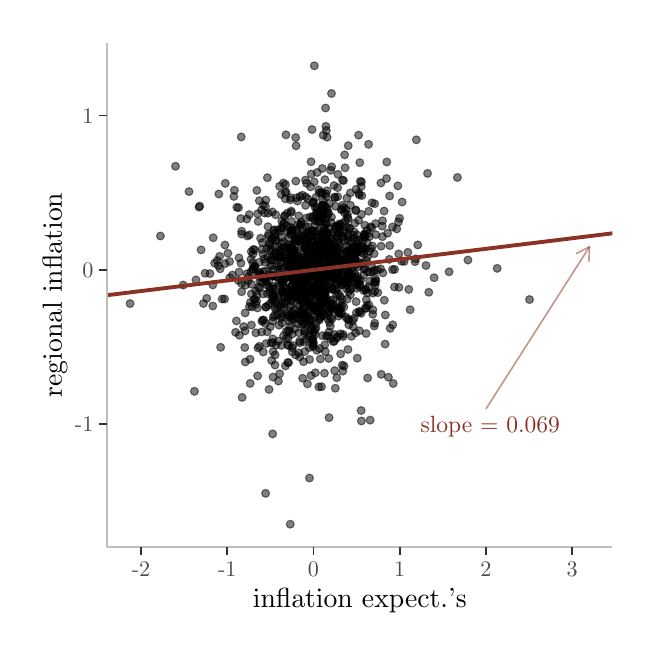
\begin{tikzpicture}[x=1pt,y=1pt]
\definecolor{fillColor}{RGB}{255,255,255}
\path[use as bounding box,fill=fillColor,fill opacity=0.00] (0,0) rectangle (216.81,216.81);
\begin{scope}
\path[clip] (  0.00,  0.00) rectangle (216.81,216.81);
\definecolor{drawColor}{RGB}{255,255,255}
\definecolor{fillColor}{RGB}{255,255,255}

\path[draw=drawColor,line width= 0.6pt,line join=round,line cap=round,fill=fillColor] (  0.00,  0.00) rectangle (216.81,216.81);
\end{scope}
\begin{scope}
\path[clip] ( 28.70, 29.10) rectangle (211.31,211.31);
\definecolor{drawColor}{RGB}{255,255,255}

\path[draw=drawColor,line width= 0.6pt,line join=round] ( 28.70, 73.48) --
	(211.31, 73.48);

\path[draw=drawColor,line width= 0.6pt,line join=round] ( 28.70,129.27) --
	(211.31,129.27);

\path[draw=drawColor,line width= 0.6pt,line join=round] ( 28.70,185.06) --
	(211.31,185.06);

\path[draw=drawColor,line width= 0.6pt,line join=round] ( 40.96, 29.10) --
	( 40.96,211.31);

\path[draw=drawColor,line width= 0.6pt,line join=round] ( 72.12, 29.10) --
	( 72.12,211.31);

\path[draw=drawColor,line width= 0.6pt,line join=round] (103.29, 29.10) --
	(103.29,211.31);

\path[draw=drawColor,line width= 0.6pt,line join=round] (134.45, 29.10) --
	(134.45,211.31);

\path[draw=drawColor,line width= 0.6pt,line join=round] (165.61, 29.10) --
	(165.61,211.31);

\path[draw=drawColor,line width= 0.6pt,line join=round] (196.78, 29.10) --
	(196.78,211.31);
\definecolor{drawColor}{RGB}{0,0,0}
\definecolor{fillColor}{RGB}{0,0,0}

\path[draw=drawColor,draw opacity=0.50,line width= 0.4pt,line join=round,line cap=round,fill=fillColor,fill opacity=0.50] (127.53,129.69) circle (  1.43);

\path[draw=drawColor,draw opacity=0.50,line width= 0.4pt,line join=round,line cap=round,fill=fillColor,fill opacity=0.50] (118.68,117.81) circle (  1.43);

\path[draw=drawColor,draw opacity=0.50,line width= 0.4pt,line join=round,line cap=round,fill=fillColor,fill opacity=0.50] (107.37,143.39) circle (  1.43);

\path[draw=drawColor,draw opacity=0.50,line width= 0.4pt,line join=round,line cap=round,fill=fillColor,fill opacity=0.50] (130.05,142.54) circle (  1.43);

\path[draw=drawColor,draw opacity=0.50,line width= 0.4pt,line join=round,line cap=round,fill=fillColor,fill opacity=0.50] ( 86.44,123.78) circle (  1.43);

\path[draw=drawColor,draw opacity=0.50,line width= 0.4pt,line join=round,line cap=round,fill=fillColor,fill opacity=0.50] (104.52,132.90) circle (  1.43);

\path[draw=drawColor,draw opacity=0.50,line width= 0.4pt,line join=round,line cap=round,fill=fillColor,fill opacity=0.50] (109.44,133.29) circle (  1.43);

\path[draw=drawColor,draw opacity=0.50,line width= 0.4pt,line join=round,line cap=round,fill=fillColor,fill opacity=0.50] (112.29,130.18) circle (  1.43);

\path[draw=drawColor,draw opacity=0.50,line width= 0.4pt,line join=round,line cap=round,fill=fillColor,fill opacity=0.50] ( 66.88,123.85) circle (  1.43);

\path[draw=drawColor,draw opacity=0.50,line width= 0.4pt,line join=round,line cap=round,fill=fillColor,fill opacity=0.50] (108.87,114.10) circle (  1.43);

\path[draw=drawColor,draw opacity=0.50,line width= 0.4pt,line join=round,line cap=round,fill=fillColor,fill opacity=0.50] ( 67.56,131.72) circle (  1.43);

\path[draw=drawColor,draw opacity=0.50,line width= 0.4pt,line join=round,line cap=round,fill=fillColor,fill opacity=0.50] ( 99.79,127.98) circle (  1.43);

\path[draw=drawColor,draw opacity=0.50,line width= 0.4pt,line join=round,line cap=round,fill=fillColor,fill opacity=0.50] (106.67,148.41) circle (  1.43);

\path[draw=drawColor,draw opacity=0.50,line width= 0.4pt,line join=round,line cap=round,fill=fillColor,fill opacity=0.50] (111.89,105.17) circle (  1.43);

\path[draw=drawColor,draw opacity=0.50,line width= 0.4pt,line join=round,line cap=round,fill=fillColor,fill opacity=0.50] (100.01,140.46) circle (  1.43);

\path[draw=drawColor,draw opacity=0.50,line width= 0.4pt,line join=round,line cap=round,fill=fillColor,fill opacity=0.50] (105.33,125.35) circle (  1.43);

\path[draw=drawColor,draw opacity=0.50,line width= 0.4pt,line join=round,line cap=round,fill=fillColor,fill opacity=0.50] (102.88,105.69) circle (  1.43);

\path[draw=drawColor,draw opacity=0.50,line width= 0.4pt,line join=round,line cap=round,fill=fillColor,fill opacity=0.50] (100.97,139.45) circle (  1.43);

\path[draw=drawColor,draw opacity=0.50,line width= 0.4pt,line join=round,line cap=round,fill=fillColor,fill opacity=0.50] ( 53.42,166.72) circle (  1.43);

\path[draw=drawColor,draw opacity=0.50,line width= 0.4pt,line join=round,line cap=round,fill=fillColor,fill opacity=0.50] (115.30,126.23) circle (  1.43);

\path[draw=drawColor,draw opacity=0.50,line width= 0.4pt,line join=round,line cap=round,fill=fillColor,fill opacity=0.50] (122.30,106.28) circle (  1.43);

\path[draw=drawColor,draw opacity=0.50,line width= 0.4pt,line join=round,line cap=round,fill=fillColor,fill opacity=0.50] (134.09,135.05) circle (  1.43);

\path[draw=drawColor,draw opacity=0.50,line width= 0.4pt,line join=round,line cap=round,fill=fillColor,fill opacity=0.50] (117.01,122.76) circle (  1.43);

\path[draw=drawColor,draw opacity=0.50,line width= 0.4pt,line join=round,line cap=round,fill=fillColor,fill opacity=0.50] ( 69.55,129.67) circle (  1.43);

\path[draw=drawColor,draw opacity=0.50,line width= 0.4pt,line join=round,line cap=round,fill=fillColor,fill opacity=0.50] (137.37,135.62) circle (  1.43);

\path[draw=drawColor,draw opacity=0.50,line width= 0.4pt,line join=round,line cap=round,fill=fillColor,fill opacity=0.50] ( 77.32,121.38) circle (  1.43);

\path[draw=drawColor,draw opacity=0.50,line width= 0.4pt,line join=round,line cap=round,fill=fillColor,fill opacity=0.50] (105.12,126.94) circle (  1.43);

\path[draw=drawColor,draw opacity=0.50,line width= 0.4pt,line join=round,line cap=round,fill=fillColor,fill opacity=0.50] (119.38,124.53) circle (  1.43);

\path[draw=drawColor,draw opacity=0.50,line width= 0.4pt,line join=round,line cap=round,fill=fillColor,fill opacity=0.50] ( 97.98,141.95) circle (  1.43);

\path[draw=drawColor,draw opacity=0.50,line width= 0.4pt,line join=round,line cap=round,fill=fillColor,fill opacity=0.50] ( 88.32,127.28) circle (  1.43);

\path[draw=drawColor,draw opacity=0.50,line width= 0.4pt,line join=round,line cap=round,fill=fillColor,fill opacity=0.50] (118.39,134.80) circle (  1.43);

\path[draw=drawColor,draw opacity=0.50,line width= 0.4pt,line join=round,line cap=round,fill=fillColor,fill opacity=0.50] ( 82.40,121.64) circle (  1.43);

\path[draw=drawColor,draw opacity=0.50,line width= 0.4pt,line join=round,line cap=round,fill=fillColor,fill opacity=0.50] ( 69.35,134.18) circle (  1.43);

\path[draw=drawColor,draw opacity=0.50,line width= 0.4pt,line join=round,line cap=round,fill=fillColor,fill opacity=0.50] ( 71.37,131.57) circle (  1.43);

\path[draw=drawColor,draw opacity=0.50,line width= 0.4pt,line join=round,line cap=round,fill=fillColor,fill opacity=0.50] ( 62.17,152.33) circle (  1.43);

\path[draw=drawColor,draw opacity=0.50,line width= 0.4pt,line join=round,line cap=round,fill=fillColor,fill opacity=0.50] ( 97.62,132.94) circle (  1.43);

\path[draw=drawColor,draw opacity=0.50,line width= 0.4pt,line join=round,line cap=round,fill=fillColor,fill opacity=0.50] ( 60.81,125.67) circle (  1.43);

\path[draw=drawColor,draw opacity=0.50,line width= 0.4pt,line join=round,line cap=round,fill=fillColor,fill opacity=0.50] (117.69,133.68) circle (  1.43);

\path[draw=drawColor,draw opacity=0.50,line width= 0.4pt,line join=round,line cap=round,fill=fillColor,fill opacity=0.50] (122.92,142.34) circle (  1.43);

\path[draw=drawColor,draw opacity=0.50,line width= 0.4pt,line join=round,line cap=round,fill=fillColor,fill opacity=0.50] (126.39,129.28) circle (  1.43);

\path[draw=drawColor,draw opacity=0.50,line width= 0.4pt,line join=round,line cap=round,fill=fillColor,fill opacity=0.50] ( 94.63,110.68) circle (  1.43);

\path[draw=drawColor,draw opacity=0.50,line width= 0.4pt,line join=round,line cap=round,fill=fillColor,fill opacity=0.50] (109.63,115.28) circle (  1.43);

\path[draw=drawColor,draw opacity=0.50,line width= 0.4pt,line join=round,line cap=round,fill=fillColor,fill opacity=0.50] (181.33,118.57) circle (  1.43);

\path[draw=drawColor,draw opacity=0.50,line width= 0.4pt,line join=round,line cap=round,fill=fillColor,fill opacity=0.50] (125.53,124.71) circle (  1.43);

\path[draw=drawColor,draw opacity=0.50,line width= 0.4pt,line join=round,line cap=round,fill=fillColor,fill opacity=0.50] (112.50,145.87) circle (  1.43);

\path[draw=drawColor,draw opacity=0.50,line width= 0.4pt,line join=round,line cap=round,fill=fillColor,fill opacity=0.50] ( 96.37,129.74) circle (  1.43);

\path[draw=drawColor,draw opacity=0.50,line width= 0.4pt,line join=round,line cap=round,fill=fillColor,fill opacity=0.50] ( 77.30,142.23) circle (  1.43);

\path[draw=drawColor,draw opacity=0.50,line width= 0.4pt,line join=round,line cap=round,fill=fillColor,fill opacity=0.50] ( 81.40,134.97) circle (  1.43);

\path[draw=drawColor,draw opacity=0.50,line width= 0.4pt,line join=round,line cap=round,fill=fillColor,fill opacity=0.50] ( 87.02,141.52) circle (  1.43);

\path[draw=drawColor,draw opacity=0.50,line width= 0.4pt,line join=round,line cap=round,fill=fillColor,fill opacity=0.50] (114.63,128.45) circle (  1.43);

\path[draw=drawColor,draw opacity=0.50,line width= 0.4pt,line join=round,line cap=round,fill=fillColor,fill opacity=0.50] ( 95.94,122.05) circle (  1.43);

\path[draw=drawColor,draw opacity=0.50,line width= 0.4pt,line join=round,line cap=round,fill=fillColor,fill opacity=0.50] (103.79,133.38) circle (  1.43);

\path[draw=drawColor,draw opacity=0.50,line width= 0.4pt,line join=round,line cap=round,fill=fillColor,fill opacity=0.50] (122.17,122.20) circle (  1.43);

\path[draw=drawColor,draw opacity=0.50,line width= 0.4pt,line join=round,line cap=round,fill=fillColor,fill opacity=0.50] (112.42,113.66) circle (  1.43);

\path[draw=drawColor,draw opacity=0.50,line width= 0.4pt,line join=round,line cap=round,fill=fillColor,fill opacity=0.50] (120.36,125.64) circle (  1.43);

\path[draw=drawColor,draw opacity=0.50,line width= 0.4pt,line join=round,line cap=round,fill=fillColor,fill opacity=0.50] (115.53,111.50) circle (  1.43);

\path[draw=drawColor,draw opacity=0.50,line width= 0.4pt,line join=round,line cap=round,fill=fillColor,fill opacity=0.50] (118.12,134.10) circle (  1.43);

\path[draw=drawColor,draw opacity=0.50,line width= 0.4pt,line join=round,line cap=round,fill=fillColor,fill opacity=0.50] (107.63,119.91) circle (  1.43);

\path[draw=drawColor,draw opacity=0.50,line width= 0.4pt,line join=round,line cap=round,fill=fillColor,fill opacity=0.50] ( 74.00,127.41) circle (  1.43);

\path[draw=drawColor,draw opacity=0.50,line width= 0.4pt,line join=round,line cap=round,fill=fillColor,fill opacity=0.50] (101.23,136.38) circle (  1.43);

\path[draw=drawColor,draw opacity=0.50,line width= 0.4pt,line join=round,line cap=round,fill=fillColor,fill opacity=0.50] ( 56.21,123.80) circle (  1.43);

\path[draw=drawColor,draw opacity=0.50,line width= 0.4pt,line join=round,line cap=round,fill=fillColor,fill opacity=0.50] (146.86,126.47) circle (  1.43);

\path[draw=drawColor,draw opacity=0.50,line width= 0.4pt,line join=round,line cap=round,fill=fillColor,fill opacity=0.50] (104.79,114.86) circle (  1.43);

\path[draw=drawColor,draw opacity=0.50,line width= 0.4pt,line join=round,line cap=round,fill=fillColor,fill opacity=0.50] (119.63,157.02) circle (  1.43);

\path[draw=drawColor,draw opacity=0.50,line width= 0.4pt,line join=round,line cap=round,fill=fillColor,fill opacity=0.50] ( 73.03,126.43) circle (  1.43);

\path[draw=drawColor,draw opacity=0.50,line width= 0.4pt,line join=round,line cap=round,fill=fillColor,fill opacity=0.50] ( 96.69,132.21) circle (  1.43);

\path[draw=drawColor,draw opacity=0.50,line width= 0.4pt,line join=round,line cap=round,fill=fillColor,fill opacity=0.50] (105.22,120.31) circle (  1.43);

\path[draw=drawColor,draw opacity=0.50,line width= 0.4pt,line join=round,line cap=round,fill=fillColor,fill opacity=0.50] (136.02,132.33) circle (  1.43);

\path[draw=drawColor,draw opacity=0.50,line width= 0.4pt,line join=round,line cap=round,fill=fillColor,fill opacity=0.50] (115.08,112.19) circle (  1.43);

\path[draw=drawColor,draw opacity=0.50,line width= 0.4pt,line join=round,line cap=round,fill=fillColor,fill opacity=0.50] (120.95,136.25) circle (  1.43);

\path[draw=drawColor,draw opacity=0.50,line width= 0.4pt,line join=round,line cap=round,fill=fillColor,fill opacity=0.50] ( 76.36,133.61) circle (  1.43);

\path[draw=drawColor,draw opacity=0.50,line width= 0.4pt,line join=round,line cap=round,fill=fillColor,fill opacity=0.50] (100.75,135.02) circle (  1.43);

\path[draw=drawColor,draw opacity=0.50,line width= 0.4pt,line join=round,line cap=round,fill=fillColor,fill opacity=0.50] ( 88.89,143.45) circle (  1.43);

\path[draw=drawColor,draw opacity=0.50,line width= 0.4pt,line join=round,line cap=round,fill=fillColor,fill opacity=0.50] (120.02,123.95) circle (  1.43);

\path[draw=drawColor,draw opacity=0.50,line width= 0.4pt,line join=round,line cap=round,fill=fillColor,fill opacity=0.50] ( 98.68,118.70) circle (  1.43);

\path[draw=drawColor,draw opacity=0.50,line width= 0.4pt,line join=round,line cap=round,fill=fillColor,fill opacity=0.50] (105.56,130.97) circle (  1.43);

\path[draw=drawColor,draw opacity=0.50,line width= 0.4pt,line join=round,line cap=round,fill=fillColor,fill opacity=0.50] (117.42,110.95) circle (  1.43);

\path[draw=drawColor,draw opacity=0.50,line width= 0.4pt,line join=round,line cap=round,fill=fillColor,fill opacity=0.50] (125.42,129.16) circle (  1.43);

\path[draw=drawColor,draw opacity=0.50,line width= 0.4pt,line join=round,line cap=round,fill=fillColor,fill opacity=0.50] ( 87.63,138.24) circle (  1.43);

\path[draw=drawColor,draw opacity=0.50,line width= 0.4pt,line join=round,line cap=round,fill=fillColor,fill opacity=0.50] (125.86,125.42) circle (  1.43);

\path[draw=drawColor,draw opacity=0.50,line width= 0.4pt,line join=round,line cap=round,fill=fillColor,fill opacity=0.50] (131.92,109.44) circle (  1.43);

\path[draw=drawColor,draw opacity=0.50,line width= 0.4pt,line join=round,line cap=round,fill=fillColor,fill opacity=0.50] ( 92.95,126.84) circle (  1.43);

\path[draw=drawColor,draw opacity=0.50,line width= 0.4pt,line join=round,line cap=round,fill=fillColor,fill opacity=0.50] ( 80.68,128.50) circle (  1.43);

\path[draw=drawColor,draw opacity=0.50,line width= 0.4pt,line join=round,line cap=round,fill=fillColor,fill opacity=0.50] ( 94.44,131.34) circle (  1.43);

\path[draw=drawColor,draw opacity=0.50,line width= 0.4pt,line join=round,line cap=round,fill=fillColor,fill opacity=0.50] ( 98.85,130.18) circle (  1.43);

\path[draw=drawColor,draw opacity=0.50,line width= 0.4pt,line join=round,line cap=round,fill=fillColor,fill opacity=0.50] (100.53,144.91) circle (  1.43);

\path[draw=drawColor,draw opacity=0.50,line width= 0.4pt,line join=round,line cap=round,fill=fillColor,fill opacity=0.50] ( 89.38,135.35) circle (  1.43);

\path[draw=drawColor,draw opacity=0.50,line width= 0.4pt,line join=round,line cap=round,fill=fillColor,fill opacity=0.50] ( 94.36,140.88) circle (  1.43);

\path[draw=drawColor,draw opacity=0.50,line width= 0.4pt,line join=round,line cap=round,fill=fillColor,fill opacity=0.50] (104.06,132.28) circle (  1.43);

\path[draw=drawColor,draw opacity=0.50,line width= 0.4pt,line join=round,line cap=round,fill=fillColor,fill opacity=0.50] ( 86.08,128.75) circle (  1.43);

\path[draw=drawColor,draw opacity=0.50,line width= 0.4pt,line join=round,line cap=round,fill=fillColor,fill opacity=0.50] (115.91,127.88) circle (  1.43);

\path[draw=drawColor,draw opacity=0.50,line width= 0.4pt,line join=round,line cap=round,fill=fillColor,fill opacity=0.50] ( 64.11,128.06) circle (  1.43);

\path[draw=drawColor,draw opacity=0.50,line width= 0.4pt,line join=round,line cap=round,fill=fillColor,fill opacity=0.50] (114.73,133.45) circle (  1.43);

\path[draw=drawColor,draw opacity=0.50,line width= 0.4pt,line join=round,line cap=round,fill=fillColor,fill opacity=0.50] (100.92,143.12) circle (  1.43);

\path[draw=drawColor,draw opacity=0.50,line width= 0.4pt,line join=round,line cap=round,fill=fillColor,fill opacity=0.50] ( 94.60,136.81) circle (  1.43);

\path[draw=drawColor,draw opacity=0.50,line width= 0.4pt,line join=round,line cap=round,fill=fillColor,fill opacity=0.50] (110.31,118.54) circle (  1.43);

\path[draw=drawColor,draw opacity=0.50,line width= 0.4pt,line join=round,line cap=round,fill=fillColor,fill opacity=0.50] (115.14,122.58) circle (  1.43);

\path[draw=drawColor,draw opacity=0.50,line width= 0.4pt,line join=round,line cap=round,fill=fillColor,fill opacity=0.50] (112.37,120.66) circle (  1.43);

\path[draw=drawColor,draw opacity=0.50,line width= 0.4pt,line join=round,line cap=round,fill=fillColor,fill opacity=0.50] (111.23,126.10) circle (  1.43);

\path[draw=drawColor,draw opacity=0.50,line width= 0.4pt,line join=round,line cap=round,fill=fillColor,fill opacity=0.50] (109.96,132.99) circle (  1.43);

\path[draw=drawColor,draw opacity=0.50,line width= 0.4pt,line join=round,line cap=round,fill=fillColor,fill opacity=0.50] ( 97.72,128.89) circle (  1.43);

\path[draw=drawColor,draw opacity=0.50,line width= 0.4pt,line join=round,line cap=round,fill=fillColor,fill opacity=0.50] ( 86.58,106.89) circle (  1.43);

\path[draw=drawColor,draw opacity=0.50,line width= 0.4pt,line join=round,line cap=round,fill=fillColor,fill opacity=0.50] ( 87.25,123.16) circle (  1.43);

\path[draw=drawColor,draw opacity=0.50,line width= 0.4pt,line join=round,line cap=round,fill=fillColor,fill opacity=0.50] ( 99.67,117.62) circle (  1.43);

\path[draw=drawColor,draw opacity=0.50,line width= 0.4pt,line join=round,line cap=round,fill=fillColor,fill opacity=0.50] (122.77,120.95) circle (  1.43);

\path[draw=drawColor,draw opacity=0.50,line width= 0.4pt,line join=round,line cap=round,fill=fillColor,fill opacity=0.50] (108.18,157.89) circle (  1.43);

\path[draw=drawColor,draw opacity=0.50,line width= 0.4pt,line join=round,line cap=round,fill=fillColor,fill opacity=0.50] (114.60,139.57) circle (  1.43);

\path[draw=drawColor,draw opacity=0.50,line width= 0.4pt,line join=round,line cap=round,fill=fillColor,fill opacity=0.50] (121.80,136.78) circle (  1.43);

\path[draw=drawColor,draw opacity=0.50,line width= 0.4pt,line join=round,line cap=round,fill=fillColor,fill opacity=0.50] (115.99,121.45) circle (  1.43);

\path[draw=drawColor,draw opacity=0.50,line width= 0.4pt,line join=round,line cap=round,fill=fillColor,fill opacity=0.50] ( 87.85,136.93) circle (  1.43);

\path[draw=drawColor,draw opacity=0.50,line width= 0.4pt,line join=round,line cap=round,fill=fillColor,fill opacity=0.50] (109.87,122.25) circle (  1.43);

\path[draw=drawColor,draw opacity=0.50,line width= 0.4pt,line join=round,line cap=round,fill=fillColor,fill opacity=0.50] ( 87.16,138.84) circle (  1.43);

\path[draw=drawColor,draw opacity=0.50,line width= 0.4pt,line join=round,line cap=round,fill=fillColor,fill opacity=0.50] (100.95,140.89) circle (  1.43);

\path[draw=drawColor,draw opacity=0.50,line width= 0.4pt,line join=round,line cap=round,fill=fillColor,fill opacity=0.50] (103.86,133.96) circle (  1.43);

\path[draw=drawColor,draw opacity=0.50,line width= 0.4pt,line join=round,line cap=round,fill=fillColor,fill opacity=0.50] (117.75,134.27) circle (  1.43);

\path[draw=drawColor,draw opacity=0.50,line width= 0.4pt,line join=round,line cap=round,fill=fillColor,fill opacity=0.50] ( 85.49,133.25) circle (  1.43);

\path[draw=drawColor,draw opacity=0.50,line width= 0.4pt,line join=round,line cap=round,fill=fillColor,fill opacity=0.50] ( 94.45,130.58) circle (  1.43);

\path[draw=drawColor,draw opacity=0.50,line width= 0.4pt,line join=round,line cap=round,fill=fillColor,fill opacity=0.50] ( 81.32,129.48) circle (  1.43);

\path[draw=drawColor,draw opacity=0.50,line width= 0.4pt,line join=round,line cap=round,fill=fillColor,fill opacity=0.50] (106.97,113.09) circle (  1.43);

\path[draw=drawColor,draw opacity=0.50,line width= 0.4pt,line join=round,line cap=round,fill=fillColor,fill opacity=0.50] (128.20,141.29) circle (  1.43);

\path[draw=drawColor,draw opacity=0.50,line width= 0.4pt,line join=round,line cap=round,fill=fillColor,fill opacity=0.50] ( 90.24,112.97) circle (  1.43);

\path[draw=drawColor,draw opacity=0.50,line width= 0.4pt,line join=round,line cap=round,fill=fillColor,fill opacity=0.50] (109.20,130.99) circle (  1.43);

\path[draw=drawColor,draw opacity=0.50,line width= 0.4pt,line join=round,line cap=round,fill=fillColor,fill opacity=0.50] ( 99.56,120.90) circle (  1.43);

\path[draw=drawColor,draw opacity=0.50,line width= 0.4pt,line join=round,line cap=round,fill=fillColor,fill opacity=0.50] (121.43,129.56) circle (  1.43);

\path[draw=drawColor,draw opacity=0.50,line width= 0.4pt,line join=round,line cap=round,fill=fillColor,fill opacity=0.50] (115.72,141.64) circle (  1.43);

\path[draw=drawColor,draw opacity=0.50,line width= 0.4pt,line join=round,line cap=round,fill=fillColor,fill opacity=0.50] (100.70,148.01) circle (  1.43);

\path[draw=drawColor,draw opacity=0.50,line width= 0.4pt,line join=round,line cap=round,fill=fillColor,fill opacity=0.50] (114.74,127.27) circle (  1.43);

\path[draw=drawColor,draw opacity=0.50,line width= 0.4pt,line join=round,line cap=round,fill=fillColor,fill opacity=0.50] (109.59,136.12) circle (  1.43);

\path[draw=drawColor,draw opacity=0.50,line width= 0.4pt,line join=round,line cap=round,fill=fillColor,fill opacity=0.50] (112.29,136.62) circle (  1.43);

\path[draw=drawColor,draw opacity=0.50,line width= 0.4pt,line join=round,line cap=round,fill=fillColor,fill opacity=0.50] (121.43,121.79) circle (  1.43);

\path[draw=drawColor,draw opacity=0.50,line width= 0.4pt,line join=round,line cap=round,fill=fillColor,fill opacity=0.50] (115.89,132.81) circle (  1.43);

\path[draw=drawColor,draw opacity=0.50,line width= 0.4pt,line join=round,line cap=round,fill=fillColor,fill opacity=0.50] ( 97.91,123.86) circle (  1.43);

\path[draw=drawColor,draw opacity=0.50,line width= 0.4pt,line join=round,line cap=round,fill=fillColor,fill opacity=0.50] ( 80.86,124.10) circle (  1.43);

\path[draw=drawColor,draw opacity=0.50,line width= 0.4pt,line join=round,line cap=round,fill=fillColor,fill opacity=0.50] ( 88.97,118.50) circle (  1.43);

\path[draw=drawColor,draw opacity=0.50,line width= 0.4pt,line join=round,line cap=round,fill=fillColor,fill opacity=0.50] ( 66.89,116.24) circle (  1.43);

\path[draw=drawColor,draw opacity=0.50,line width= 0.4pt,line join=round,line cap=round,fill=fillColor,fill opacity=0.50] (114.44,124.27) circle (  1.43);

\path[draw=drawColor,draw opacity=0.50,line width= 0.4pt,line join=round,line cap=round,fill=fillColor,fill opacity=0.50] ( 91.46,115.93) circle (  1.43);

\path[draw=drawColor,draw opacity=0.50,line width= 0.4pt,line join=round,line cap=round,fill=fillColor,fill opacity=0.50] ( 93.35,132.33) circle (  1.43);

\path[draw=drawColor,draw opacity=0.50,line width= 0.4pt,line join=round,line cap=round,fill=fillColor,fill opacity=0.50] (106.18,135.78) circle (  1.43);

\path[draw=drawColor,draw opacity=0.50,line width= 0.4pt,line join=round,line cap=round,fill=fillColor,fill opacity=0.50] (117.56,137.33) circle (  1.43);

\path[draw=drawColor,draw opacity=0.50,line width= 0.4pt,line join=round,line cap=round,fill=fillColor,fill opacity=0.50] (115.81,124.46) circle (  1.43);

\path[draw=drawColor,draw opacity=0.50,line width= 0.4pt,line join=round,line cap=round,fill=fillColor,fill opacity=0.50] ( 91.62,111.85) circle (  1.43);

\path[draw=drawColor,draw opacity=0.50,line width= 0.4pt,line join=round,line cap=round,fill=fillColor,fill opacity=0.50] (119.68,130.54) circle (  1.43);

\path[draw=drawColor,draw opacity=0.50,line width= 0.4pt,line join=round,line cap=round,fill=fillColor,fill opacity=0.50] ( 87.84,136.09) circle (  1.43);

\path[draw=drawColor,draw opacity=0.50,line width= 0.4pt,line join=round,line cap=round,fill=fillColor,fill opacity=0.50] (106.70,129.45) circle (  1.43);

\path[draw=drawColor,draw opacity=0.50,line width= 0.4pt,line join=round,line cap=round,fill=fillColor,fill opacity=0.50] ( 91.60,135.85) circle (  1.43);

\path[draw=drawColor,draw opacity=0.50,line width= 0.4pt,line join=round,line cap=round,fill=fillColor,fill opacity=0.50] (101.57,134.11) circle (  1.43);

\path[draw=drawColor,draw opacity=0.50,line width= 0.4pt,line join=round,line cap=round,fill=fillColor,fill opacity=0.50] (116.06,127.49) circle (  1.43);

\path[draw=drawColor,draw opacity=0.50,line width= 0.4pt,line join=round,line cap=round,fill=fillColor,fill opacity=0.50] ( 99.67,128.59) circle (  1.43);

\path[draw=drawColor,draw opacity=0.50,line width= 0.4pt,line join=round,line cap=round,fill=fillColor,fill opacity=0.50] (113.04,145.64) circle (  1.43);

\path[draw=drawColor,draw opacity=0.50,line width= 0.4pt,line join=round,line cap=round,fill=fillColor,fill opacity=0.50] ( 83.84,128.06) circle (  1.43);

\path[draw=drawColor,draw opacity=0.50,line width= 0.4pt,line join=round,line cap=round,fill=fillColor,fill opacity=0.50] (128.80,150.55) circle (  1.43);

\path[draw=drawColor,draw opacity=0.50,line width= 0.4pt,line join=round,line cap=round,fill=fillColor,fill opacity=0.50] ( 99.16,113.02) circle (  1.43);

\path[draw=drawColor,draw opacity=0.50,line width= 0.4pt,line join=round,line cap=round,fill=fillColor,fill opacity=0.50] ( 95.46,111.74) circle (  1.43);

\path[draw=drawColor,draw opacity=0.50,line width= 0.4pt,line join=round,line cap=round,fill=fillColor,fill opacity=0.50] (116.36,124.51) circle (  1.43);

\path[draw=drawColor,draw opacity=0.50,line width= 0.4pt,line join=round,line cap=round,fill=fillColor,fill opacity=0.50] (100.19,121.85) circle (  1.43);

\path[draw=drawColor,draw opacity=0.50,line width= 0.4pt,line join=round,line cap=round,fill=fillColor,fill opacity=0.50] (111.63,120.30) circle (  1.43);

\path[draw=drawColor,draw opacity=0.50,line width= 0.4pt,line join=round,line cap=round,fill=fillColor,fill opacity=0.50] (110.25,134.68) circle (  1.43);

\path[draw=drawColor,draw opacity=0.50,line width= 0.4pt,line join=round,line cap=round,fill=fillColor,fill opacity=0.50] ( 89.72,140.38) circle (  1.43);

\path[draw=drawColor,draw opacity=0.50,line width= 0.4pt,line join=round,line cap=round,fill=fillColor,fill opacity=0.50] ( 91.32,131.91) circle (  1.43);

\path[draw=drawColor,draw opacity=0.50,line width= 0.4pt,line join=round,line cap=round,fill=fillColor,fill opacity=0.50] (116.94,126.84) circle (  1.43);

\path[draw=drawColor,draw opacity=0.50,line width= 0.4pt,line join=round,line cap=round,fill=fillColor,fill opacity=0.50] ( 89.44,137.64) circle (  1.43);

\path[draw=drawColor,draw opacity=0.50,line width= 0.4pt,line join=round,line cap=round,fill=fillColor,fill opacity=0.50] ( 85.83,132.04) circle (  1.43);

\path[draw=drawColor,draw opacity=0.50,line width= 0.4pt,line join=round,line cap=round,fill=fillColor,fill opacity=0.50] (114.93,133.32) circle (  1.43);

\path[draw=drawColor,draw opacity=0.50,line width= 0.4pt,line join=round,line cap=round,fill=fillColor,fill opacity=0.50] ( 78.59,113.72) circle (  1.43);

\path[draw=drawColor,draw opacity=0.50,line width= 0.4pt,line join=round,line cap=round,fill=fillColor,fill opacity=0.50] ( 94.71,120.50) circle (  1.43);

\path[draw=drawColor,draw opacity=0.50,line width= 0.4pt,line join=round,line cap=round,fill=fillColor,fill opacity=0.50] (110.73,135.84) circle (  1.43);

\path[draw=drawColor,draw opacity=0.50,line width= 0.4pt,line join=round,line cap=round,fill=fillColor,fill opacity=0.50] ( 99.52,115.59) circle (  1.43);

\path[draw=drawColor,draw opacity=0.50,line width= 0.4pt,line join=round,line cap=round,fill=fillColor,fill opacity=0.50] (143.93,130.86) circle (  1.43);

\path[draw=drawColor,draw opacity=0.50,line width= 0.4pt,line join=round,line cap=round,fill=fillColor,fill opacity=0.50] ( 89.80,135.52) circle (  1.43);

\path[draw=drawColor,draw opacity=0.50,line width= 0.4pt,line join=round,line cap=round,fill=fillColor,fill opacity=0.50] (115.43,134.47) circle (  1.43);

\path[draw=drawColor,draw opacity=0.50,line width= 0.4pt,line join=round,line cap=round,fill=fillColor,fill opacity=0.50] ( 99.57,134.88) circle (  1.43);

\path[draw=drawColor,draw opacity=0.50,line width= 0.4pt,line join=round,line cap=round,fill=fillColor,fill opacity=0.50] ( 95.30,134.93) circle (  1.43);

\path[draw=drawColor,draw opacity=0.50,line width= 0.4pt,line join=round,line cap=round,fill=fillColor,fill opacity=0.50] (104.23,118.66) circle (  1.43);

\path[draw=drawColor,draw opacity=0.50,line width= 0.4pt,line join=round,line cap=round,fill=fillColor,fill opacity=0.50] ( 85.92,125.60) circle (  1.43);

\path[draw=drawColor,draw opacity=0.50,line width= 0.4pt,line join=round,line cap=round,fill=fillColor,fill opacity=0.50] (125.73,146.01) circle (  1.43);

\path[draw=drawColor,draw opacity=0.50,line width= 0.4pt,line join=round,line cap=round,fill=fillColor,fill opacity=0.50] (169.65,129.84) circle (  1.43);

\path[draw=drawColor,draw opacity=0.50,line width= 0.4pt,line join=round,line cap=round,fill=fillColor,fill opacity=0.50] (109.99,134.74) circle (  1.43);

\path[draw=drawColor,draw opacity=0.50,line width= 0.4pt,line join=round,line cap=round,fill=fillColor,fill opacity=0.50] ( 99.38,128.79) circle (  1.43);

\path[draw=drawColor,draw opacity=0.50,line width= 0.4pt,line join=round,line cap=round,fill=fillColor,fill opacity=0.50] (114.86,129.21) circle (  1.43);

\path[draw=drawColor,draw opacity=0.50,line width= 0.4pt,line join=round,line cap=round,fill=fillColor,fill opacity=0.50] ( 37.00,117.10) circle (  1.43);

\path[draw=drawColor,draw opacity=0.50,line width= 0.4pt,line join=round,line cap=round,fill=fillColor,fill opacity=0.50] (101.77,121.61) circle (  1.43);

\path[draw=drawColor,draw opacity=0.50,line width= 0.4pt,line join=round,line cap=round,fill=fillColor,fill opacity=0.50] ( 81.83,118.59) circle (  1.43);

\path[draw=drawColor,draw opacity=0.50,line width= 0.4pt,line join=round,line cap=round,fill=fillColor,fill opacity=0.50] (113.78,146.14) circle (  1.43);

\path[draw=drawColor,draw opacity=0.50,line width= 0.4pt,line join=round,line cap=round,fill=fillColor,fill opacity=0.50] (104.76,141.99) circle (  1.43);

\path[draw=drawColor,draw opacity=0.50,line width= 0.4pt,line join=round,line cap=round,fill=fillColor,fill opacity=0.50] ( 94.42,132.97) circle (  1.43);

\path[draw=drawColor,draw opacity=0.50,line width= 0.4pt,line join=round,line cap=round,fill=fillColor,fill opacity=0.50] ( 96.85,121.09) circle (  1.43);

\path[draw=drawColor,draw opacity=0.50,line width= 0.4pt,line join=round,line cap=round,fill=fillColor,fill opacity=0.50] (110.92,128.99) circle (  1.43);

\path[draw=drawColor,draw opacity=0.50,line width= 0.4pt,line join=round,line cap=round,fill=fillColor,fill opacity=0.50] ( 99.54,122.61) circle (  1.43);

\path[draw=drawColor,draw opacity=0.50,line width= 0.4pt,line join=round,line cap=round,fill=fillColor,fill opacity=0.50] ( 92.72,133.81) circle (  1.43);

\path[draw=drawColor,draw opacity=0.50,line width= 0.4pt,line join=round,line cap=round,fill=fillColor,fill opacity=0.50] (105.99,128.20) circle (  1.43);

\path[draw=drawColor,draw opacity=0.50,line width= 0.4pt,line join=round,line cap=round,fill=fillColor,fill opacity=0.50] (112.37,114.82) circle (  1.43);

\path[draw=drawColor,draw opacity=0.50,line width= 0.4pt,line join=round,line cap=round,fill=fillColor,fill opacity=0.50] (118.67,131.28) circle (  1.43);

\path[draw=drawColor,draw opacity=0.50,line width= 0.4pt,line join=round,line cap=round,fill=fillColor,fill opacity=0.50] ( 91.77,125.28) circle (  1.43);

\path[draw=drawColor,draw opacity=0.50,line width= 0.4pt,line join=round,line cap=round,fill=fillColor,fill opacity=0.50] ( 90.19,132.59) circle (  1.43);

\path[draw=drawColor,draw opacity=0.50,line width= 0.4pt,line join=round,line cap=round,fill=fillColor,fill opacity=0.50] (121.23,137.60) circle (  1.43);

\path[draw=drawColor,draw opacity=0.50,line width= 0.4pt,line join=round,line cap=round,fill=fillColor,fill opacity=0.50] (122.55,116.29) circle (  1.43);

\path[draw=drawColor,draw opacity=0.50,line width= 0.4pt,line join=round,line cap=round,fill=fillColor,fill opacity=0.50] (106.52,129.11) circle (  1.43);

\path[draw=drawColor,draw opacity=0.50,line width= 0.4pt,line join=round,line cap=round,fill=fillColor,fill opacity=0.50] ( 83.65,127.58) circle (  1.43);

\path[draw=drawColor,draw opacity=0.50,line width= 0.4pt,line join=round,line cap=round,fill=fillColor,fill opacity=0.50] (124.76,114.84) circle (  1.43);

\path[draw=drawColor,draw opacity=0.50,line width= 0.4pt,line join=round,line cap=round,fill=fillColor,fill opacity=0.50] (112.67,138.33) circle (  1.43);

\path[draw=drawColor,draw opacity=0.50,line width= 0.4pt,line join=round,line cap=round,fill=fillColor,fill opacity=0.50] (118.52,150.75) circle (  1.43);

\path[draw=drawColor,draw opacity=0.50,line width= 0.4pt,line join=round,line cap=round,fill=fillColor,fill opacity=0.50] ( 76.37,128.49) circle (  1.43);

\path[draw=drawColor,draw opacity=0.50,line width= 0.4pt,line join=round,line cap=round,fill=fillColor,fill opacity=0.50] (104.83,133.65) circle (  1.43);

\path[draw=drawColor,draw opacity=0.50,line width= 0.4pt,line join=round,line cap=round,fill=fillColor,fill opacity=0.50] ( 95.68,114.02) circle (  1.43);

\path[draw=drawColor,draw opacity=0.50,line width= 0.4pt,line join=round,line cap=round,fill=fillColor,fill opacity=0.50] ( 94.99,138.07) circle (  1.43);

\path[draw=drawColor,draw opacity=0.50,line width= 0.4pt,line join=round,line cap=round,fill=fillColor,fill opacity=0.50] ( 88.18,133.99) circle (  1.43);

\path[draw=drawColor,draw opacity=0.50,line width= 0.4pt,line join=round,line cap=round,fill=fillColor,fill opacity=0.50] (110.72,126.12) circle (  1.43);

\path[draw=drawColor,draw opacity=0.50,line width= 0.4pt,line join=round,line cap=round,fill=fillColor,fill opacity=0.50] (110.48,133.66) circle (  1.43);

\path[draw=drawColor,draw opacity=0.50,line width= 0.4pt,line join=round,line cap=round,fill=fillColor,fill opacity=0.50] (118.23,132.03) circle (  1.43);

\path[draw=drawColor,draw opacity=0.50,line width= 0.4pt,line join=round,line cap=round,fill=fillColor,fill opacity=0.50] (128.36,128.20) circle (  1.43);

\path[draw=drawColor,draw opacity=0.50,line width= 0.4pt,line join=round,line cap=round,fill=fillColor,fill opacity=0.50] (103.73,131.46) circle (  1.43);

\path[draw=drawColor,draw opacity=0.50,line width= 0.4pt,line join=round,line cap=round,fill=fillColor,fill opacity=0.50] (104.71,131.30) circle (  1.43);

\path[draw=drawColor,draw opacity=0.50,line width= 0.4pt,line join=round,line cap=round,fill=fillColor,fill opacity=0.50] (115.22,135.53) circle (  1.43);

\path[draw=drawColor,draw opacity=0.50,line width= 0.4pt,line join=round,line cap=round,fill=fillColor,fill opacity=0.50] ( 77.09,131.70) circle (  1.43);

\path[draw=drawColor,draw opacity=0.50,line width= 0.4pt,line join=round,line cap=round,fill=fillColor,fill opacity=0.50] (107.34,140.86) circle (  1.43);

\path[draw=drawColor,draw opacity=0.50,line width= 0.4pt,line join=round,line cap=round,fill=fillColor,fill opacity=0.50] ( 93.18,133.39) circle (  1.43);

\path[draw=drawColor,draw opacity=0.50,line width= 0.4pt,line join=round,line cap=round,fill=fillColor,fill opacity=0.50] ( 88.54,104.35) circle (  1.43);

\path[draw=drawColor,draw opacity=0.50,line width= 0.4pt,line join=round,line cap=round,fill=fillColor,fill opacity=0.50] (103.19,133.34) circle (  1.43);

\path[draw=drawColor,draw opacity=0.50,line width= 0.4pt,line join=round,line cap=round,fill=fillColor,fill opacity=0.50] ( 89.36,115.39) circle (  1.43);

\path[draw=drawColor,draw opacity=0.50,line width= 0.4pt,line join=round,line cap=round,fill=fillColor,fill opacity=0.50] (107.77,128.69) circle (  1.43);

\path[draw=drawColor,draw opacity=0.50,line width= 0.4pt,line join=round,line cap=round,fill=fillColor,fill opacity=0.50] (100.54,128.09) circle (  1.43);

\path[draw=drawColor,draw opacity=0.50,line width= 0.4pt,line join=round,line cap=round,fill=fillColor,fill opacity=0.50] ( 90.81,133.88) circle (  1.43);

\path[draw=drawColor,draw opacity=0.50,line width= 0.4pt,line join=round,line cap=round,fill=fillColor,fill opacity=0.50] ( 97.48,126.13) circle (  1.43);

\path[draw=drawColor,draw opacity=0.50,line width= 0.4pt,line join=round,line cap=round,fill=fillColor,fill opacity=0.50] (108.63,123.01) circle (  1.43);

\path[draw=drawColor,draw opacity=0.50,line width= 0.4pt,line join=round,line cap=round,fill=fillColor,fill opacity=0.50] (107.97,127.79) circle (  1.43);

\path[draw=drawColor,draw opacity=0.50,line width= 0.4pt,line join=round,line cap=round,fill=fillColor,fill opacity=0.50] (100.43,125.65) circle (  1.43);

\path[draw=drawColor,draw opacity=0.50,line width= 0.4pt,line join=round,line cap=round,fill=fillColor,fill opacity=0.50] (123.16,123.21) circle (  1.43);

\path[draw=drawColor,draw opacity=0.50,line width= 0.4pt,line join=round,line cap=round,fill=fillColor,fill opacity=0.50] (110.17,130.65) circle (  1.43);

\path[draw=drawColor,draw opacity=0.50,line width= 0.4pt,line join=round,line cap=round,fill=fillColor,fill opacity=0.50] (102.76,139.12) circle (  1.43);

\path[draw=drawColor,draw opacity=0.50,line width= 0.4pt,line join=round,line cap=round,fill=fillColor,fill opacity=0.50] ( 84.16,140.74) circle (  1.43);

\path[draw=drawColor,draw opacity=0.50,line width= 0.4pt,line join=round,line cap=round,fill=fillColor,fill opacity=0.50] (105.55,124.26) circle (  1.43);

\path[draw=drawColor,draw opacity=0.50,line width= 0.4pt,line join=round,line cap=round,fill=fillColor,fill opacity=0.50] (121.92,115.39) circle (  1.43);

\path[draw=drawColor,draw opacity=0.50,line width= 0.4pt,line join=round,line cap=round,fill=fillColor,fill opacity=0.50] ( 75.42,110.84) circle (  1.43);

\path[draw=drawColor,draw opacity=0.50,line width= 0.4pt,line join=round,line cap=round,fill=fillColor,fill opacity=0.50] (106.12,146.86) circle (  1.43);

\path[draw=drawColor,draw opacity=0.50,line width= 0.4pt,line join=round,line cap=round,fill=fillColor,fill opacity=0.50] ( 89.85,126.87) circle (  1.43);

\path[draw=drawColor,draw opacity=0.50,line width= 0.4pt,line join=round,line cap=round,fill=fillColor,fill opacity=0.50] ( 96.26,136.33) circle (  1.43);

\path[draw=drawColor,draw opacity=0.50,line width= 0.4pt,line join=round,line cap=round,fill=fillColor,fill opacity=0.50] (117.99,142.99) circle (  1.43);

\path[draw=drawColor,draw opacity=0.50,line width= 0.4pt,line join=round,line cap=round,fill=fillColor,fill opacity=0.50] (114.83,125.76) circle (  1.43);

\path[draw=drawColor,draw opacity=0.50,line width= 0.4pt,line join=round,line cap=round,fill=fillColor,fill opacity=0.50] ( 85.21,126.58) circle (  1.43);

\path[draw=drawColor,draw opacity=0.50,line width= 0.4pt,line join=round,line cap=round,fill=fillColor,fill opacity=0.50] (101.59,128.51) circle (  1.43);

\path[draw=drawColor,draw opacity=0.50,line width= 0.4pt,line join=round,line cap=round,fill=fillColor,fill opacity=0.50] (110.00,122.70) circle (  1.43);

\path[draw=drawColor,draw opacity=0.50,line width= 0.4pt,line join=round,line cap=round,fill=fillColor,fill opacity=0.50] (108.45,139.26) circle (  1.43);

\path[draw=drawColor,draw opacity=0.50,line width= 0.4pt,line join=round,line cap=round,fill=fillColor,fill opacity=0.50] (111.80,129.15) circle (  1.43);

\path[draw=drawColor,draw opacity=0.50,line width= 0.4pt,line join=round,line cap=round,fill=fillColor,fill opacity=0.50] (102.75,143.54) circle (  1.43);

\path[draw=drawColor,draw opacity=0.50,line width= 0.4pt,line join=round,line cap=round,fill=fillColor,fill opacity=0.50] (102.45,131.56) circle (  1.43);

\path[draw=drawColor,draw opacity=0.50,line width= 0.4pt,line join=round,line cap=round,fill=fillColor,fill opacity=0.50] ( 95.44,134.77) circle (  1.43);

\path[draw=drawColor,draw opacity=0.50,line width= 0.4pt,line join=round,line cap=round,fill=fillColor,fill opacity=0.50] (101.54,132.61) circle (  1.43);

\path[draw=drawColor,draw opacity=0.50,line width= 0.4pt,line join=round,line cap=round,fill=fillColor,fill opacity=0.50] (106.10,136.55) circle (  1.43);

\path[draw=drawColor,draw opacity=0.50,line width= 0.4pt,line join=round,line cap=round,fill=fillColor,fill opacity=0.50] (114.26,115.93) circle (  1.43);

\path[draw=drawColor,draw opacity=0.50,line width= 0.4pt,line join=round,line cap=round,fill=fillColor,fill opacity=0.50] ( 99.64,128.16) circle (  1.43);

\path[draw=drawColor,draw opacity=0.50,line width= 0.4pt,line join=round,line cap=round,fill=fillColor,fill opacity=0.50] (103.32,129.28) circle (  1.43);

\path[draw=drawColor,draw opacity=0.50,line width= 0.4pt,line join=round,line cap=round,fill=fillColor,fill opacity=0.50] ( 93.08,157.27) circle (  1.43);

\path[draw=drawColor,draw opacity=0.50,line width= 0.4pt,line join=round,line cap=round,fill=fillColor,fill opacity=0.50] (100.77,104.12) circle (  1.43);

\path[draw=drawColor,draw opacity=0.50,line width= 0.4pt,line join=round,line cap=round,fill=fillColor,fill opacity=0.50] (116.55,122.22) circle (  1.43);

\path[draw=drawColor,draw opacity=0.50,line width= 0.4pt,line join=round,line cap=round,fill=fillColor,fill opacity=0.50] (103.52,115.21) circle (  1.43);

\path[draw=drawColor,draw opacity=0.50,line width= 0.4pt,line join=round,line cap=round,fill=fillColor,fill opacity=0.50] ( 81.32,131.81) circle (  1.43);

\path[draw=drawColor,draw opacity=0.50,line width= 0.4pt,line join=round,line cap=round,fill=fillColor,fill opacity=0.50] (116.15,134.93) circle (  1.43);

\path[draw=drawColor,draw opacity=0.50,line width= 0.4pt,line join=round,line cap=round,fill=fillColor,fill opacity=0.50] (104.14,133.25) circle (  1.43);

\path[draw=drawColor,draw opacity=0.50,line width= 0.4pt,line join=round,line cap=round,fill=fillColor,fill opacity=0.50] (109.33,128.90) circle (  1.43);

\path[draw=drawColor,draw opacity=0.50,line width= 0.4pt,line join=round,line cap=round,fill=fillColor,fill opacity=0.50] (117.53,135.62) circle (  1.43);

\path[draw=drawColor,draw opacity=0.50,line width= 0.4pt,line join=round,line cap=round,fill=fillColor,fill opacity=0.50] ( 86.46,126.76) circle (  1.43);

\path[draw=drawColor,draw opacity=0.50,line width= 0.4pt,line join=round,line cap=round,fill=fillColor,fill opacity=0.50] (101.41,122.32) circle (  1.43);

\path[draw=drawColor,draw opacity=0.50,line width= 0.4pt,line join=round,line cap=round,fill=fillColor,fill opacity=0.50] ( 99.08,127.83) circle (  1.43);

\path[draw=drawColor,draw opacity=0.50,line width= 0.4pt,line join=round,line cap=round,fill=fillColor,fill opacity=0.50] (106.97,119.03) circle (  1.43);

\path[draw=drawColor,draw opacity=0.50,line width= 0.4pt,line join=round,line cap=round,fill=fillColor,fill opacity=0.50] (106.67,140.45) circle (  1.43);

\path[draw=drawColor,draw opacity=0.50,line width= 0.4pt,line join=round,line cap=round,fill=fillColor,fill opacity=0.50] (104.34,121.51) circle (  1.43);

\path[draw=drawColor,draw opacity=0.50,line width= 0.4pt,line join=round,line cap=round,fill=fillColor,fill opacity=0.50] (106.03,128.81) circle (  1.43);

\path[draw=drawColor,draw opacity=0.50,line width= 0.4pt,line join=round,line cap=round,fill=fillColor,fill opacity=0.50] ( 90.66,124.53) circle (  1.43);

\path[draw=drawColor,draw opacity=0.50,line width= 0.4pt,line join=round,line cap=round,fill=fillColor,fill opacity=0.50] ( 96.16,135.87) circle (  1.43);

\path[draw=drawColor,draw opacity=0.50,line width= 0.4pt,line join=round,line cap=round,fill=fillColor,fill opacity=0.50] (103.61,136.18) circle (  1.43);

\path[draw=drawColor,draw opacity=0.50,line width= 0.4pt,line join=round,line cap=round,fill=fillColor,fill opacity=0.50] ( 98.65,124.75) circle (  1.43);

\path[draw=drawColor,draw opacity=0.50,line width= 0.4pt,line join=round,line cap=round,fill=fillColor,fill opacity=0.50] (111.74,141.49) circle (  1.43);

\path[draw=drawColor,draw opacity=0.50,line width= 0.4pt,line join=round,line cap=round,fill=fillColor,fill opacity=0.50] (103.71,132.32) circle (  1.43);

\path[draw=drawColor,draw opacity=0.50,line width= 0.4pt,line join=round,line cap=round,fill=fillColor,fill opacity=0.50] (117.05,130.07) circle (  1.43);

\path[draw=drawColor,draw opacity=0.50,line width= 0.4pt,line join=round,line cap=round,fill=fillColor,fill opacity=0.50] ( 96.83,130.98) circle (  1.43);

\path[draw=drawColor,draw opacity=0.50,line width= 0.4pt,line join=round,line cap=round,fill=fillColor,fill opacity=0.50] ( 96.95,128.03) circle (  1.43);

\path[draw=drawColor,draw opacity=0.50,line width= 0.4pt,line join=round,line cap=round,fill=fillColor,fill opacity=0.50] (111.21,121.88) circle (  1.43);

\path[draw=drawColor,draw opacity=0.50,line width= 0.4pt,line join=round,line cap=round,fill=fillColor,fill opacity=0.50] (106.53,126.60) circle (  1.43);

\path[draw=drawColor,draw opacity=0.50,line width= 0.4pt,line join=round,line cap=round,fill=fillColor,fill opacity=0.50] (106.34,118.53) circle (  1.43);

\path[draw=drawColor,draw opacity=0.50,line width= 0.4pt,line join=round,line cap=round,fill=fillColor,fill opacity=0.50] (123.99,137.03) circle (  1.43);

\path[draw=drawColor,draw opacity=0.50,line width= 0.4pt,line join=round,line cap=round,fill=fillColor,fill opacity=0.50] ( 98.67,145.49) circle (  1.43);

\path[draw=drawColor,draw opacity=0.50,line width= 0.4pt,line join=round,line cap=round,fill=fillColor,fill opacity=0.50] ( 94.22,119.21) circle (  1.43);

\path[draw=drawColor,draw opacity=0.50,line width= 0.4pt,line join=round,line cap=round,fill=fillColor,fill opacity=0.50] (116.17,135.67) circle (  1.43);

\path[draw=drawColor,draw opacity=0.50,line width= 0.4pt,line join=round,line cap=round,fill=fillColor,fill opacity=0.50] (108.95,140.61) circle (  1.43);

\path[draw=drawColor,draw opacity=0.50,line width= 0.4pt,line join=round,line cap=round,fill=fillColor,fill opacity=0.50] ( 88.71, 99.78) circle (  1.43);

\path[draw=drawColor,draw opacity=0.50,line width= 0.4pt,line join=round,line cap=round,fill=fillColor,fill opacity=0.50] (102.84,143.20) circle (  1.43);

\path[draw=drawColor,draw opacity=0.50,line width= 0.4pt,line join=round,line cap=round,fill=fillColor,fill opacity=0.50] (109.82,132.94) circle (  1.43);

\path[draw=drawColor,draw opacity=0.50,line width= 0.4pt,line join=round,line cap=round,fill=fillColor,fill opacity=0.50] ( 95.13,130.67) circle (  1.43);

\path[draw=drawColor,draw opacity=0.50,line width= 0.4pt,line join=round,line cap=round,fill=fillColor,fill opacity=0.50] (107.38,137.10) circle (  1.43);

\path[draw=drawColor,draw opacity=0.50,line width= 0.4pt,line join=round,line cap=round,fill=fillColor,fill opacity=0.50] (105.73,112.25) circle (  1.43);

\path[draw=drawColor,draw opacity=0.50,line width= 0.4pt,line join=round,line cap=round,fill=fillColor,fill opacity=0.50] ( 87.82,117.28) circle (  1.43);

\path[draw=drawColor,draw opacity=0.50,line width= 0.4pt,line join=round,line cap=round,fill=fillColor,fill opacity=0.50] ( 88.85,119.71) circle (  1.43);

\path[draw=drawColor,draw opacity=0.50,line width= 0.4pt,line join=round,line cap=round,fill=fillColor,fill opacity=0.50] (109.41,130.76) circle (  1.43);

\path[draw=drawColor,draw opacity=0.50,line width= 0.4pt,line join=round,line cap=round,fill=fillColor,fill opacity=0.50] (108.44,142.51) circle (  1.43);

\path[draw=drawColor,draw opacity=0.50,line width= 0.4pt,line join=round,line cap=round,fill=fillColor,fill opacity=0.50] (101.98,127.85) circle (  1.43);

\path[draw=drawColor,draw opacity=0.50,line width= 0.4pt,line join=round,line cap=round,fill=fillColor,fill opacity=0.50] (109.76,137.40) circle (  1.43);

\path[draw=drawColor,draw opacity=0.50,line width= 0.4pt,line join=round,line cap=round,fill=fillColor,fill opacity=0.50] ( 95.81,126.46) circle (  1.43);

\path[draw=drawColor,draw opacity=0.50,line width= 0.4pt,line join=round,line cap=round,fill=fillColor,fill opacity=0.50] ( 94.10,131.18) circle (  1.43);

\path[draw=drawColor,draw opacity=0.50,line width= 0.4pt,line join=round,line cap=round,fill=fillColor,fill opacity=0.50] (101.76,111.23) circle (  1.43);

\path[draw=drawColor,draw opacity=0.50,line width= 0.4pt,line join=round,line cap=round,fill=fillColor,fill opacity=0.50] (104.19,126.99) circle (  1.43);

\path[draw=drawColor,draw opacity=0.50,line width= 0.4pt,line join=round,line cap=round,fill=fillColor,fill opacity=0.50] (103.97,131.13) circle (  1.43);

\path[draw=drawColor,draw opacity=0.50,line width= 0.4pt,line join=round,line cap=round,fill=fillColor,fill opacity=0.50] ( 97.73,130.10) circle (  1.43);

\path[draw=drawColor,draw opacity=0.50,line width= 0.4pt,line join=round,line cap=round,fill=fillColor,fill opacity=0.50] (123.42,135.91) circle (  1.43);

\path[draw=drawColor,draw opacity=0.50,line width= 0.4pt,line join=round,line cap=round,fill=fillColor,fill opacity=0.50] (111.31,145.03) circle (  1.43);

\path[draw=drawColor,draw opacity=0.50,line width= 0.4pt,line join=round,line cap=round,fill=fillColor,fill opacity=0.50] (109.25,134.27) circle (  1.43);

\path[draw=drawColor,draw opacity=0.50,line width= 0.4pt,line join=round,line cap=round,fill=fillColor,fill opacity=0.50] (106.04,117.99) circle (  1.43);

\path[draw=drawColor,draw opacity=0.50,line width= 0.4pt,line join=round,line cap=round,fill=fillColor,fill opacity=0.50] ( 83.87,122.86) circle (  1.43);

\path[draw=drawColor,draw opacity=0.50,line width= 0.4pt,line join=round,line cap=round,fill=fillColor,fill opacity=0.50] (100.66,141.85) circle (  1.43);

\path[draw=drawColor,draw opacity=0.50,line width= 0.4pt,line join=round,line cap=round,fill=fillColor,fill opacity=0.50] (101.59,119.22) circle (  1.43);

\path[draw=drawColor,draw opacity=0.50,line width= 0.4pt,line join=round,line cap=round,fill=fillColor,fill opacity=0.50] (115.73,125.55) circle (  1.43);

\path[draw=drawColor,draw opacity=0.50,line width= 0.4pt,line join=round,line cap=round,fill=fillColor,fill opacity=0.50] ( 98.50,118.28) circle (  1.43);

\path[draw=drawColor,draw opacity=0.50,line width= 0.4pt,line join=round,line cap=round,fill=fillColor,fill opacity=0.50] (104.62,139.35) circle (  1.43);

\path[draw=drawColor,draw opacity=0.50,line width= 0.4pt,line join=round,line cap=round,fill=fillColor,fill opacity=0.50] ( 99.08,127.49) circle (  1.43);

\path[draw=drawColor,draw opacity=0.50,line width= 0.4pt,line join=round,line cap=round,fill=fillColor,fill opacity=0.50] (113.54,130.57) circle (  1.43);

\path[draw=drawColor,draw opacity=0.50,line width= 0.4pt,line join=round,line cap=round,fill=fillColor,fill opacity=0.50] ( 95.26,128.76) circle (  1.43);

\path[draw=drawColor,draw opacity=0.50,line width= 0.4pt,line join=round,line cap=round,fill=fillColor,fill opacity=0.50] ( 96.85,177.09) circle (  1.43);

\path[draw=drawColor,draw opacity=0.50,line width= 0.4pt,line join=round,line cap=round,fill=fillColor,fill opacity=0.50] (102.83,142.39) circle (  1.43);

\path[draw=drawColor,draw opacity=0.50,line width= 0.4pt,line join=round,line cap=round,fill=fillColor,fill opacity=0.50] (111.90,141.15) circle (  1.43);

\path[draw=drawColor,draw opacity=0.50,line width= 0.4pt,line join=round,line cap=round,fill=fillColor,fill opacity=0.50] (116.68,141.03) circle (  1.43);

\path[draw=drawColor,draw opacity=0.50,line width= 0.4pt,line join=round,line cap=round,fill=fillColor,fill opacity=0.50] ( 90.57,103.59) circle (  1.43);

\path[draw=drawColor,draw opacity=0.50,line width= 0.4pt,line join=round,line cap=round,fill=fillColor,fill opacity=0.50] (114.00,105.95) circle (  1.43);

\path[draw=drawColor,draw opacity=0.50,line width= 0.4pt,line join=round,line cap=round,fill=fillColor,fill opacity=0.50] (112.39,125.55) circle (  1.43);

\path[draw=drawColor,draw opacity=0.50,line width= 0.4pt,line join=round,line cap=round,fill=fillColor,fill opacity=0.50] ( 85.96,115.84) circle (  1.43);

\path[draw=drawColor,draw opacity=0.50,line width= 0.4pt,line join=round,line cap=round,fill=fillColor,fill opacity=0.50] ( 90.46,129.36) circle (  1.43);

\path[draw=drawColor,draw opacity=0.50,line width= 0.4pt,line join=round,line cap=round,fill=fillColor,fill opacity=0.50] ( 96.14,125.48) circle (  1.43);

\path[draw=drawColor,draw opacity=0.50,line width= 0.4pt,line join=round,line cap=round,fill=fillColor,fill opacity=0.50] (108.18,130.04) circle (  1.43);

\path[draw=drawColor,draw opacity=0.50,line width= 0.4pt,line join=round,line cap=round,fill=fillColor,fill opacity=0.50] (113.47,113.74) circle (  1.43);

\path[draw=drawColor,draw opacity=0.50,line width= 0.4pt,line join=round,line cap=round,fill=fillColor,fill opacity=0.50] ( 96.07,136.40) circle (  1.43);

\path[draw=drawColor,draw opacity=0.50,line width= 0.4pt,line join=round,line cap=round,fill=fillColor,fill opacity=0.50] (109.64,117.17) circle (  1.43);

\path[draw=drawColor,draw opacity=0.50,line width= 0.4pt,line join=round,line cap=round,fill=fillColor,fill opacity=0.50] (101.89,116.85) circle (  1.43);

\path[draw=drawColor,draw opacity=0.50,line width= 0.4pt,line join=round,line cap=round,fill=fillColor,fill opacity=0.50] ( 88.76,120.41) circle (  1.43);

\path[draw=drawColor,draw opacity=0.50,line width= 0.4pt,line join=round,line cap=round,fill=fillColor,fill opacity=0.50] ( 87.22,125.47) circle (  1.43);

\path[draw=drawColor,draw opacity=0.50,line width= 0.4pt,line join=round,line cap=round,fill=fillColor,fill opacity=0.50] (108.16,138.55) circle (  1.43);

\path[draw=drawColor,draw opacity=0.50,line width= 0.4pt,line join=round,line cap=round,fill=fillColor,fill opacity=0.50] (106.94,119.16) circle (  1.43);

\path[draw=drawColor,draw opacity=0.50,line width= 0.4pt,line join=round,line cap=round,fill=fillColor,fill opacity=0.50] (103.95,120.87) circle (  1.43);

\path[draw=drawColor,draw opacity=0.50,line width= 0.4pt,line join=round,line cap=round,fill=fillColor,fill opacity=0.50] (101.98,134.52) circle (  1.43);

\path[draw=drawColor,draw opacity=0.50,line width= 0.4pt,line join=round,line cap=round,fill=fillColor,fill opacity=0.50] (116.35,144.19) circle (  1.43);

\path[draw=drawColor,draw opacity=0.50,line width= 0.4pt,line join=round,line cap=round,fill=fillColor,fill opacity=0.50] (112.89,142.26) circle (  1.43);

\path[draw=drawColor,draw opacity=0.50,line width= 0.4pt,line join=round,line cap=round,fill=fillColor,fill opacity=0.50] (105.59,135.37) circle (  1.43);

\path[draw=drawColor,draw opacity=0.50,line width= 0.4pt,line join=round,line cap=round,fill=fillColor,fill opacity=0.50] (103.96,133.51) circle (  1.43);

\path[draw=drawColor,draw opacity=0.50,line width= 0.4pt,line join=round,line cap=round,fill=fillColor,fill opacity=0.50] ( 96.03,120.67) circle (  1.43);

\path[draw=drawColor,draw opacity=0.50,line width= 0.4pt,line join=round,line cap=round,fill=fillColor,fill opacity=0.50] (113.13,124.90) circle (  1.43);

\path[draw=drawColor,draw opacity=0.50,line width= 0.4pt,line join=round,line cap=round,fill=fillColor,fill opacity=0.50] (111.59,123.97) circle (  1.43);

\path[draw=drawColor,draw opacity=0.50,line width= 0.4pt,line join=round,line cap=round,fill=fillColor,fill opacity=0.50] (107.30,122.48) circle (  1.43);

\path[draw=drawColor,draw opacity=0.50,line width= 0.4pt,line join=round,line cap=round,fill=fillColor,fill opacity=0.50] ( 91.73,141.13) circle (  1.43);

\path[draw=drawColor,draw opacity=0.50,line width= 0.4pt,line join=round,line cap=round,fill=fillColor,fill opacity=0.50] (104.30,136.06) circle (  1.43);

\path[draw=drawColor,draw opacity=0.50,line width= 0.4pt,line join=round,line cap=round,fill=fillColor,fill opacity=0.50] ( 98.24,131.43) circle (  1.43);

\path[draw=drawColor,draw opacity=0.50,line width= 0.4pt,line join=round,line cap=round,fill=fillColor,fill opacity=0.50] ( 92.03,129.86) circle (  1.43);

\path[draw=drawColor,draw opacity=0.50,line width= 0.4pt,line join=round,line cap=round,fill=fillColor,fill opacity=0.50] ( 97.77,125.64) circle (  1.43);

\path[draw=drawColor,draw opacity=0.50,line width= 0.4pt,line join=round,line cap=round,fill=fillColor,fill opacity=0.50] (119.82,124.96) circle (  1.43);

\path[draw=drawColor,draw opacity=0.50,line width= 0.4pt,line join=round,line cap=round,fill=fillColor,fill opacity=0.50] (103.53,136.62) circle (  1.43);

\path[draw=drawColor,draw opacity=0.50,line width= 0.4pt,line join=round,line cap=round,fill=fillColor,fill opacity=0.50] (108.91, 75.89) circle (  1.43);

\path[draw=drawColor,draw opacity=0.50,line width= 0.4pt,line join=round,line cap=round,fill=fillColor,fill opacity=0.50] (102.38, 91.10) circle (  1.43);

\path[draw=drawColor,draw opacity=0.50,line width= 0.4pt,line join=round,line cap=round,fill=fillColor,fill opacity=0.50] (103.05,104.18) circle (  1.43);

\path[draw=drawColor,draw opacity=0.50,line width= 0.4pt,line join=round,line cap=round,fill=fillColor,fill opacity=0.50] ( 94.17,107.35) circle (  1.43);

\path[draw=drawColor,draw opacity=0.50,line width= 0.4pt,line join=round,line cap=round,fill=fillColor,fill opacity=0.50] (101.99,141.64) circle (  1.43);

\path[draw=drawColor,draw opacity=0.50,line width= 0.4pt,line join=round,line cap=round,fill=fillColor,fill opacity=0.50] ( 98.68,145.92) circle (  1.43);

\path[draw=drawColor,draw opacity=0.50,line width= 0.4pt,line join=round,line cap=round,fill=fillColor,fill opacity=0.50] (123.75,128.44) circle (  1.43);

\path[draw=drawColor,draw opacity=0.50,line width= 0.4pt,line join=round,line cap=round,fill=fillColor,fill opacity=0.50] (101.10,128.95) circle (  1.43);

\path[draw=drawColor,draw opacity=0.50,line width= 0.4pt,line join=round,line cap=round,fill=fillColor,fill opacity=0.50] ( 92.41,145.90) circle (  1.43);

\path[draw=drawColor,draw opacity=0.50,line width= 0.4pt,line join=round,line cap=round,fill=fillColor,fill opacity=0.50] (109.78,193.03) circle (  1.43);

\path[draw=drawColor,draw opacity=0.50,line width= 0.4pt,line join=round,line cap=round,fill=fillColor,fill opacity=0.50] ( 98.74,137.30) circle (  1.43);

\path[draw=drawColor,draw opacity=0.50,line width= 0.4pt,line join=round,line cap=round,fill=fillColor,fill opacity=0.50] (104.48,151.54) circle (  1.43);

\path[draw=drawColor,draw opacity=0.50,line width= 0.4pt,line join=round,line cap=round,fill=fillColor,fill opacity=0.50] (121.12,139.75) circle (  1.43);

\path[draw=drawColor,draw opacity=0.50,line width= 0.4pt,line join=round,line cap=round,fill=fillColor,fill opacity=0.50] ( 86.17,102.66) circle (  1.43);

\path[draw=drawColor,draw opacity=0.50,line width= 0.4pt,line join=round,line cap=round,fill=fillColor,fill opacity=0.50] (115.77,139.92) circle (  1.43);

\path[draw=drawColor,draw opacity=0.50,line width= 0.4pt,line join=round,line cap=round,fill=fillColor,fill opacity=0.50] ( 88.54,132.81) circle (  1.43);

\path[draw=drawColor,draw opacity=0.50,line width= 0.4pt,line join=round,line cap=round,fill=fillColor,fill opacity=0.50] (102.42,138.35) circle (  1.43);

\path[draw=drawColor,draw opacity=0.50,line width= 0.4pt,line join=round,line cap=round,fill=fillColor,fill opacity=0.50] ( 99.79,109.87) circle (  1.43);

\path[draw=drawColor,draw opacity=0.50,line width= 0.4pt,line join=round,line cap=round,fill=fillColor,fill opacity=0.50] ( 86.20,115.88) circle (  1.43);

\path[draw=drawColor,draw opacity=0.50,line width= 0.4pt,line join=round,line cap=round,fill=fillColor,fill opacity=0.50] (110.16,122.50) circle (  1.43);

\path[draw=drawColor,draw opacity=0.50,line width= 0.4pt,line join=round,line cap=round,fill=fillColor,fill opacity=0.50] (101.44,135.83) circle (  1.43);

\path[draw=drawColor,draw opacity=0.50,line width= 0.4pt,line join=round,line cap=round,fill=fillColor,fill opacity=0.50] (113.32,151.06) circle (  1.43);

\path[draw=drawColor,draw opacity=0.50,line width= 0.4pt,line join=round,line cap=round,fill=fillColor,fill opacity=0.50] ( 91.65,134.05) circle (  1.43);

\path[draw=drawColor,draw opacity=0.50,line width= 0.4pt,line join=round,line cap=round,fill=fillColor,fill opacity=0.50] (122.86,128.55) circle (  1.43);

\path[draw=drawColor,draw opacity=0.50,line width= 0.4pt,line join=round,line cap=round,fill=fillColor,fill opacity=0.50] (125.79,142.03) circle (  1.43);

\path[draw=drawColor,draw opacity=0.50,line width= 0.4pt,line join=round,line cap=round,fill=fillColor,fill opacity=0.50] (120.63,135.56) circle (  1.43);

\path[draw=drawColor,draw opacity=0.50,line width= 0.4pt,line join=round,line cap=round,fill=fillColor,fill opacity=0.50] (128.87,118.32) circle (  1.43);

\path[draw=drawColor,draw opacity=0.50,line width= 0.4pt,line join=round,line cap=round,fill=fillColor,fill opacity=0.50] (103.68,114.62) circle (  1.43);

\path[draw=drawColor,draw opacity=0.50,line width= 0.4pt,line join=round,line cap=round,fill=fillColor,fill opacity=0.50] (100.88,136.33) circle (  1.43);

\path[draw=drawColor,draw opacity=0.50,line width= 0.4pt,line join=round,line cap=round,fill=fillColor,fill opacity=0.50] ( 96.71,131.27) circle (  1.43);

\path[draw=drawColor,draw opacity=0.50,line width= 0.4pt,line join=round,line cap=round,fill=fillColor,fill opacity=0.50] (118.19,135.49) circle (  1.43);

\path[draw=drawColor,draw opacity=0.50,line width= 0.4pt,line join=round,line cap=round,fill=fillColor,fill opacity=0.50] (110.98,132.88) circle (  1.43);

\path[draw=drawColor,draw opacity=0.50,line width= 0.4pt,line join=round,line cap=round,fill=fillColor,fill opacity=0.50] ( 88.85,129.33) circle (  1.43);

\path[draw=drawColor,draw opacity=0.50,line width= 0.4pt,line join=round,line cap=round,fill=fillColor,fill opacity=0.50] ( 67.03,140.89) circle (  1.43);

\path[draw=drawColor,draw opacity=0.50,line width= 0.4pt,line join=round,line cap=round,fill=fillColor,fill opacity=0.50] ( 64.70,118.99) circle (  1.43);

\path[draw=drawColor,draw opacity=0.50,line width= 0.4pt,line join=round,line cap=round,fill=fillColor,fill opacity=0.50] (113.11,115.51) circle (  1.43);

\path[draw=drawColor,draw opacity=0.50,line width= 0.4pt,line join=round,line cap=round,fill=fillColor,fill opacity=0.50] (133.76,159.64) circle (  1.43);

\path[draw=drawColor,draw opacity=0.50,line width= 0.4pt,line join=round,line cap=round,fill=fillColor,fill opacity=0.50] (102.75,179.99) circle (  1.43);

\path[draw=drawColor,draw opacity=0.50,line width= 0.4pt,line join=round,line cap=round,fill=fillColor,fill opacity=0.50] (119.21,131.51) circle (  1.43);

\path[draw=drawColor,draw opacity=0.50,line width= 0.4pt,line join=round,line cap=round,fill=fillColor,fill opacity=0.50] (107.03,139.82) circle (  1.43);

\path[draw=drawColor,draw opacity=0.50,line width= 0.4pt,line join=round,line cap=round,fill=fillColor,fill opacity=0.50] (102.58,141.99) circle (  1.43);

\path[draw=drawColor,draw opacity=0.50,line width= 0.4pt,line join=round,line cap=round,fill=fillColor,fill opacity=0.50] ( 83.86,125.24) circle (  1.43);

\path[draw=drawColor,draw opacity=0.50,line width= 0.4pt,line join=round,line cap=round,fill=fillColor,fill opacity=0.50] ( 82.45,106.54) circle (  1.43);

\path[draw=drawColor,draw opacity=0.50,line width= 0.4pt,line join=round,line cap=round,fill=fillColor,fill opacity=0.50] (110.90,138.54) circle (  1.43);

\path[draw=drawColor,draw opacity=0.50,line width= 0.4pt,line join=round,line cap=round,fill=fillColor,fill opacity=0.50] (102.81,115.95) circle (  1.43);

\path[draw=drawColor,draw opacity=0.50,line width= 0.4pt,line join=round,line cap=round,fill=fillColor,fill opacity=0.50] (110.93, 92.89) circle (  1.43);

\path[draw=drawColor,draw opacity=0.50,line width= 0.4pt,line join=round,line cap=round,fill=fillColor,fill opacity=0.50] (102.76,130.86) circle (  1.43);

\path[draw=drawColor,draw opacity=0.50,line width= 0.4pt,line join=round,line cap=round,fill=fillColor,fill opacity=0.50] ( 80.39, 88.26) circle (  1.43);

\path[draw=drawColor,draw opacity=0.50,line width= 0.4pt,line join=round,line cap=round,fill=fillColor,fill opacity=0.50] (118.37,133.71) circle (  1.43);

\path[draw=drawColor,draw opacity=0.50,line width= 0.4pt,line join=round,line cap=round,fill=fillColor,fill opacity=0.50] (114.13,161.56) circle (  1.43);

\path[draw=drawColor,draw opacity=0.50,line width= 0.4pt,line join=round,line cap=round,fill=fillColor,fill opacity=0.50] ( 83.78,128.41) circle (  1.43);

\path[draw=drawColor,draw opacity=0.50,line width= 0.4pt,line join=round,line cap=round,fill=fillColor,fill opacity=0.50] ( 94.58,135.18) circle (  1.43);

\path[draw=drawColor,draw opacity=0.50,line width= 0.4pt,line join=round,line cap=round,fill=fillColor,fill opacity=0.50] (106.40,152.65) circle (  1.43);

\path[draw=drawColor,draw opacity=0.50,line width= 0.4pt,line join=round,line cap=round,fill=fillColor,fill opacity=0.50] (104.22,155.59) circle (  1.43);

\path[draw=drawColor,draw opacity=0.50,line width= 0.4pt,line join=round,line cap=round,fill=fillColor,fill opacity=0.50] (104.35,131.27) circle (  1.43);

\path[draw=drawColor,draw opacity=0.50,line width= 0.4pt,line join=round,line cap=round,fill=fillColor,fill opacity=0.50] (104.88,125.12) circle (  1.43);

\path[draw=drawColor,draw opacity=0.50,line width= 0.4pt,line join=round,line cap=round,fill=fillColor,fill opacity=0.50] ( 91.19,143.16) circle (  1.43);

\path[draw=drawColor,draw opacity=0.50,line width= 0.4pt,line join=round,line cap=round,fill=fillColor,fill opacity=0.50] ( 85.97, 48.54) circle (  1.43);

\path[draw=drawColor,draw opacity=0.50,line width= 0.4pt,line join=round,line cap=round,fill=fillColor,fill opacity=0.50] (111.70,128.75) circle (  1.43);

\path[draw=drawColor,draw opacity=0.50,line width= 0.4pt,line join=round,line cap=round,fill=fillColor,fill opacity=0.50] (119.87,107.28) circle (  1.43);

\path[draw=drawColor,draw opacity=0.50,line width= 0.4pt,line join=round,line cap=round,fill=fillColor,fill opacity=0.50] ( 99.74,125.29) circle (  1.43);

\path[draw=drawColor,draw opacity=0.50,line width= 0.4pt,line join=round,line cap=round,fill=fillColor,fill opacity=0.50] (103.33,131.87) circle (  1.43);

\path[draw=drawColor,draw opacity=0.50,line width= 0.4pt,line join=round,line cap=round,fill=fillColor,fill opacity=0.50] ( 78.03,108.81) circle (  1.43);

\path[draw=drawColor,draw opacity=0.50,line width= 0.4pt,line join=round,line cap=round,fill=fillColor,fill opacity=0.50] (104.48,100.23) circle (  1.43);

\path[draw=drawColor,draw opacity=0.50,line width= 0.4pt,line join=round,line cap=round,fill=fillColor,fill opacity=0.50] (107.85,127.61) circle (  1.43);

\path[draw=drawColor,draw opacity=0.50,line width= 0.4pt,line join=round,line cap=round,fill=fillColor,fill opacity=0.50] (102.40,168.36) circle (  1.43);

\path[draw=drawColor,draw opacity=0.50,line width= 0.4pt,line join=round,line cap=round,fill=fillColor,fill opacity=0.50] (112.32,135.74) circle (  1.43);

\path[draw=drawColor,draw opacity=0.50,line width= 0.4pt,line join=round,line cap=round,fill=fillColor,fill opacity=0.50] (108.61,130.01) circle (  1.43);

\path[draw=drawColor,draw opacity=0.50,line width= 0.4pt,line join=round,line cap=round,fill=fillColor,fill opacity=0.50] ( 90.44,143.83) circle (  1.43);

\path[draw=drawColor,draw opacity=0.50,line width= 0.4pt,line join=round,line cap=round,fill=fillColor,fill opacity=0.50] (118.46,126.33) circle (  1.43);

\path[draw=drawColor,draw opacity=0.50,line width= 0.4pt,line join=round,line cap=round,fill=fillColor,fill opacity=0.50] (110.19,117.02) circle (  1.43);

\path[draw=drawColor,draw opacity=0.50,line width= 0.4pt,line join=round,line cap=round,fill=fillColor,fill opacity=0.50] (103.56,136.11) circle (  1.43);

\path[draw=drawColor,draw opacity=0.50,line width= 0.4pt,line join=round,line cap=round,fill=fillColor,fill opacity=0.50] ( 86.84,144.92) circle (  1.43);

\path[draw=drawColor,draw opacity=0.50,line width= 0.4pt,line join=round,line cap=round,fill=fillColor,fill opacity=0.50] (114.32, 94.54) circle (  1.43);

\path[draw=drawColor,draw opacity=0.50,line width= 0.4pt,line join=round,line cap=round,fill=fillColor,fill opacity=0.50] ( 85.20,128.80) circle (  1.43);

\path[draw=drawColor,draw opacity=0.50,line width= 0.4pt,line join=round,line cap=round,fill=fillColor,fill opacity=0.50] (117.26,126.97) circle (  1.43);

\path[draw=drawColor,draw opacity=0.50,line width= 0.4pt,line join=round,line cap=round,fill=fillColor,fill opacity=0.50] ( 74.71,158.06) circle (  1.43);

\path[draw=drawColor,draw opacity=0.50,line width= 0.4pt,line join=round,line cap=round,fill=fillColor,fill opacity=0.50] ( 84.73,136.69) circle (  1.43);

\path[draw=drawColor,draw opacity=0.50,line width= 0.4pt,line join=round,line cap=round,fill=fillColor,fill opacity=0.50] ( 79.70,125.38) circle (  1.43);

\path[draw=drawColor,draw opacity=0.50,line width= 0.4pt,line join=round,line cap=round,fill=fillColor,fill opacity=0.50] (103.00,121.10) circle (  1.43);

\path[draw=drawColor,draw opacity=0.50,line width= 0.4pt,line join=round,line cap=round,fill=fillColor,fill opacity=0.50] (122.55,143.57) circle (  1.43);

\path[draw=drawColor,draw opacity=0.50,line width= 0.4pt,line join=round,line cap=round,fill=fillColor,fill opacity=0.50] (137.72,122.22) circle (  1.43);

\path[draw=drawColor,draw opacity=0.50,line width= 0.4pt,line join=round,line cap=round,fill=fillColor,fill opacity=0.50] (100.86,125.88) circle (  1.43);

\path[draw=drawColor,draw opacity=0.50,line width= 0.4pt,line join=round,line cap=round,fill=fillColor,fill opacity=0.50] (132.54,123.12) circle (  1.43);

\path[draw=drawColor,draw opacity=0.50,line width= 0.4pt,line join=round,line cap=round,fill=fillColor,fill opacity=0.50] ( 99.20,132.46) circle (  1.43);

\path[draw=drawColor,draw opacity=0.50,line width= 0.4pt,line join=round,line cap=round,fill=fillColor,fill opacity=0.50] ( 87.23, 86.09) circle (  1.43);

\path[draw=drawColor,draw opacity=0.50,line width= 0.4pt,line join=round,line cap=round,fill=fillColor,fill opacity=0.50] ( 80.71,133.10) circle (  1.43);

\path[draw=drawColor,draw opacity=0.50,line width= 0.4pt,line join=round,line cap=round,fill=fillColor,fill opacity=0.50] ( 92.46,105.44) circle (  1.43);

\path[draw=drawColor,draw opacity=0.50,line width= 0.4pt,line join=round,line cap=round,fill=fillColor,fill opacity=0.50] ( 95.82,134.02) circle (  1.43);

\path[draw=drawColor,draw opacity=0.50,line width= 0.4pt,line join=round,line cap=round,fill=fillColor,fill opacity=0.50] (108.54,132.93) circle (  1.43);

\path[draw=drawColor,draw opacity=0.50,line width= 0.4pt,line join=round,line cap=round,fill=fillColor,fill opacity=0.50] ( 85.91,152.29) circle (  1.43);

\path[draw=drawColor,draw opacity=0.50,line width= 0.4pt,line join=round,line cap=round,fill=fillColor,fill opacity=0.50] (102.93,102.03) circle (  1.43);

\path[draw=drawColor,draw opacity=0.50,line width= 0.4pt,line join=round,line cap=round,fill=fillColor,fill opacity=0.50] (106.52,142.68) circle (  1.43);

\path[draw=drawColor,draw opacity=0.50,line width= 0.4pt,line join=round,line cap=round,fill=fillColor,fill opacity=0.50] (120.54,159.42) circle (  1.43);

\path[draw=drawColor,draw opacity=0.50,line width= 0.4pt,line join=round,line cap=round,fill=fillColor,fill opacity=0.50] (140.21,133.30) circle (  1.43);

\path[draw=drawColor,draw opacity=0.50,line width= 0.4pt,line join=round,line cap=round,fill=fillColor,fill opacity=0.50] (119.36,137.46) circle (  1.43);

\path[draw=drawColor,draw opacity=0.50,line width= 0.4pt,line join=round,line cap=round,fill=fillColor,fill opacity=0.50] ( 96.99,174.11) circle (  1.43);

\path[draw=drawColor,draw opacity=0.50,line width= 0.4pt,line join=round,line cap=round,fill=fillColor,fill opacity=0.50] (108.08,130.67) circle (  1.43);

\path[draw=drawColor,draw opacity=0.50,line width= 0.4pt,line join=round,line cap=round,fill=fillColor,fill opacity=0.50] ( 99.27,156.28) circle (  1.43);

\path[draw=drawColor,draw opacity=0.50,line width= 0.4pt,line join=round,line cap=round,fill=fillColor,fill opacity=0.50] (114.71,132.75) circle (  1.43);

\path[draw=drawColor,draw opacity=0.50,line width= 0.4pt,line join=round,line cap=round,fill=fillColor,fill opacity=0.50] (115.45,118.74) circle (  1.43);

\path[draw=drawColor,draw opacity=0.50,line width= 0.4pt,line join=round,line cap=round,fill=fillColor,fill opacity=0.50] (106.20, 87.07) circle (  1.43);

\path[draw=drawColor,draw opacity=0.50,line width= 0.4pt,line join=round,line cap=round,fill=fillColor,fill opacity=0.50] ( 92.74,126.00) circle (  1.43);

\path[draw=drawColor,draw opacity=0.50,line width= 0.4pt,line join=round,line cap=round,fill=fillColor,fill opacity=0.50] ( 96.52,119.48) circle (  1.43);

\path[draw=drawColor,draw opacity=0.50,line width= 0.4pt,line join=round,line cap=round,fill=fillColor,fill opacity=0.50] (100.54,111.83) circle (  1.43);

\path[draw=drawColor,draw opacity=0.50,line width= 0.4pt,line join=round,line cap=round,fill=fillColor,fill opacity=0.50] (107.24,152.40) circle (  1.43);

\path[draw=drawColor,draw opacity=0.50,line width= 0.4pt,line join=round,line cap=round,fill=fillColor,fill opacity=0.50] ( 98.52,123.83) circle (  1.43);

\path[draw=drawColor,draw opacity=0.50,line width= 0.4pt,line join=round,line cap=round,fill=fillColor,fill opacity=0.50] (103.17,118.08) circle (  1.43);

\path[draw=drawColor,draw opacity=0.50,line width= 0.4pt,line join=round,line cap=round,fill=fillColor,fill opacity=0.50] (119.22,123.73) circle (  1.43);

\path[draw=drawColor,draw opacity=0.50,line width= 0.4pt,line join=round,line cap=round,fill=fillColor,fill opacity=0.50] ( 95.02,155.38) circle (  1.43);

\path[draw=drawColor,draw opacity=0.50,line width= 0.4pt,line join=round,line cap=round,fill=fillColor,fill opacity=0.50] ( 80.12,141.94) circle (  1.43);

\path[draw=drawColor,draw opacity=0.50,line width= 0.4pt,line join=round,line cap=round,fill=fillColor,fill opacity=0.50] (105.91,132.04) circle (  1.43);

\path[draw=drawColor,draw opacity=0.50,line width= 0.4pt,line join=round,line cap=round,fill=fillColor,fill opacity=0.50] (104.42,140.86) circle (  1.43);

\path[draw=drawColor,draw opacity=0.50,line width= 0.4pt,line join=round,line cap=round,fill=fillColor,fill opacity=0.50] (105.85,125.28) circle (  1.43);

\path[draw=drawColor,draw opacity=0.50,line width= 0.4pt,line join=round,line cap=round,fill=fillColor,fill opacity=0.50] ( 86.08,154.54) circle (  1.43);

\path[draw=drawColor,draw opacity=0.50,line width= 0.4pt,line join=round,line cap=round,fill=fillColor,fill opacity=0.50] (105.59,126.70) circle (  1.43);

\path[draw=drawColor,draw opacity=0.50,line width= 0.4pt,line join=round,line cap=round,fill=fillColor,fill opacity=0.50] (106.38,117.36) circle (  1.43);

\path[draw=drawColor,draw opacity=0.50,line width= 0.4pt,line join=round,line cap=round,fill=fillColor,fill opacity=0.50] (111.16, 86.52) circle (  1.43);

\path[draw=drawColor,draw opacity=0.50,line width= 0.4pt,line join=round,line cap=round,fill=fillColor,fill opacity=0.50] (101.23,140.34) circle (  1.43);

\path[draw=drawColor,draw opacity=0.50,line width= 0.4pt,line join=round,line cap=round,fill=fillColor,fill opacity=0.50] (118.47,106.53) circle (  1.43);

\path[draw=drawColor,draw opacity=0.50,line width= 0.4pt,line join=round,line cap=round,fill=fillColor,fill opacity=0.50] (116.05,111.21) circle (  1.43);

\path[draw=drawColor,draw opacity=0.50,line width= 0.4pt,line join=round,line cap=round,fill=fillColor,fill opacity=0.50] (120.01,168.04) circle (  1.43);

\path[draw=drawColor,draw opacity=0.50,line width= 0.4pt,line join=round,line cap=round,fill=fillColor,fill opacity=0.50] ( 86.49,137.04) circle (  1.43);

\path[draw=drawColor,draw opacity=0.50,line width= 0.4pt,line join=round,line cap=round,fill=fillColor,fill opacity=0.50] (117.85,140.59) circle (  1.43);

\path[draw=drawColor,draw opacity=0.50,line width= 0.4pt,line join=round,line cap=round,fill=fillColor,fill opacity=0.50] ( 95.29,118.67) circle (  1.43);

\path[draw=drawColor,draw opacity=0.50,line width= 0.4pt,line join=round,line cap=round,fill=fillColor,fill opacity=0.50] (105.34,111.13) circle (  1.43);

\path[draw=drawColor,draw opacity=0.50,line width= 0.4pt,line join=round,line cap=round,fill=fillColor,fill opacity=0.50] (102.41,129.92) circle (  1.43);

\path[draw=drawColor,draw opacity=0.50,line width= 0.4pt,line join=round,line cap=round,fill=fillColor,fill opacity=0.50] ( 98.65,132.39) circle (  1.43);

\path[draw=drawColor,draw opacity=0.50,line width= 0.4pt,line join=round,line cap=round,fill=fillColor,fill opacity=0.50] (105.63,122.46) circle (  1.43);

\path[draw=drawColor,draw opacity=0.50,line width= 0.4pt,line join=round,line cap=round,fill=fillColor,fill opacity=0.50] (100.36,118.71) circle (  1.43);

\path[draw=drawColor,draw opacity=0.50,line width= 0.4pt,line join=round,line cap=round,fill=fillColor,fill opacity=0.50] ( 95.93,132.95) circle (  1.43);

\path[draw=drawColor,draw opacity=0.50,line width= 0.4pt,line join=round,line cap=round,fill=fillColor,fill opacity=0.50] ( 95.39,128.12) circle (  1.43);

\path[draw=drawColor,draw opacity=0.50,line width= 0.4pt,line join=round,line cap=round,fill=fillColor,fill opacity=0.50] (100.17,113.20) circle (  1.43);

\path[draw=drawColor,draw opacity=0.50,line width= 0.4pt,line join=round,line cap=round,fill=fillColor,fill opacity=0.50] ( 85.34,126.48) circle (  1.43);

\path[draw=drawColor,draw opacity=0.50,line width= 0.4pt,line join=round,line cap=round,fill=fillColor,fill opacity=0.50] ( 82.10,130.56) circle (  1.43);

\path[draw=drawColor,draw opacity=0.50,line width= 0.4pt,line join=round,line cap=round,fill=fillColor,fill opacity=0.50] ( 71.16,118.77) circle (  1.43);

\path[draw=drawColor,draw opacity=0.50,line width= 0.4pt,line join=round,line cap=round,fill=fillColor,fill opacity=0.50] (112.89,129.26) circle (  1.43);

\path[draw=drawColor,draw opacity=0.50,line width= 0.4pt,line join=round,line cap=round,fill=fillColor,fill opacity=0.50] (106.22,157.32) circle (  1.43);

\path[draw=drawColor,draw opacity=0.50,line width= 0.4pt,line join=round,line cap=round,fill=fillColor,fill opacity=0.50] ( 99.64,123.66) circle (  1.43);

\path[draw=drawColor,draw opacity=0.50,line width= 0.4pt,line join=round,line cap=round,fill=fillColor,fill opacity=0.50] (108.74,149.83) circle (  1.43);

\path[draw=drawColor,draw opacity=0.50,line width= 0.4pt,line join=round,line cap=round,fill=fillColor,fill opacity=0.50] (125.30,124.94) circle (  1.43);

\path[draw=drawColor,draw opacity=0.50,line width= 0.4pt,line join=round,line cap=round,fill=fillColor,fill opacity=0.50] (118.78,113.79) circle (  1.43);

\path[draw=drawColor,draw opacity=0.50,line width= 0.4pt,line join=round,line cap=round,fill=fillColor,fill opacity=0.50] (105.53,138.25) circle (  1.43);

\path[draw=drawColor,draw opacity=0.50,line width= 0.4pt,line join=round,line cap=round,fill=fillColor,fill opacity=0.50] (123.56,125.15) circle (  1.43);

\path[draw=drawColor,draw opacity=0.50,line width= 0.4pt,line join=round,line cap=round,fill=fillColor,fill opacity=0.50] (115.73,100.52) circle (  1.43);

\path[draw=drawColor,draw opacity=0.50,line width= 0.4pt,line join=round,line cap=round,fill=fillColor,fill opacity=0.50] ( 89.38, 94.89) circle (  1.43);

\path[draw=drawColor,draw opacity=0.50,line width= 0.4pt,line join=round,line cap=round,fill=fillColor,fill opacity=0.50] ( 91.94,121.38) circle (  1.43);

\path[draw=drawColor,draw opacity=0.50,line width= 0.4pt,line join=round,line cap=round,fill=fillColor,fill opacity=0.50] (102.18,116.55) circle (  1.43);

\path[draw=drawColor,draw opacity=0.50,line width= 0.4pt,line join=round,line cap=round,fill=fillColor,fill opacity=0.50] (131.82,144.77) circle (  1.43);

\path[draw=drawColor,draw opacity=0.50,line width= 0.4pt,line join=round,line cap=round,fill=fillColor,fill opacity=0.50] (110.46,135.63) circle (  1.43);

\path[draw=drawColor,draw opacity=0.50,line width= 0.4pt,line join=round,line cap=round,fill=fillColor,fill opacity=0.50] (108.25,151.04) circle (  1.43);

\path[draw=drawColor,draw opacity=0.50,line width= 0.4pt,line join=round,line cap=round,fill=fillColor,fill opacity=0.50] ( 97.20,127.81) circle (  1.43);

\path[draw=drawColor,draw opacity=0.50,line width= 0.4pt,line join=round,line cap=round,fill=fillColor,fill opacity=0.50] (105.20,131.71) circle (  1.43);

\path[draw=drawColor,draw opacity=0.50,line width= 0.4pt,line join=round,line cap=round,fill=fillColor,fill opacity=0.50] (104.88,141.03) circle (  1.43);

\path[draw=drawColor,draw opacity=0.50,line width= 0.4pt,line join=round,line cap=round,fill=fillColor,fill opacity=0.50] ( 92.69,145.98) circle (  1.43);

\path[draw=drawColor,draw opacity=0.50,line width= 0.4pt,line join=round,line cap=round,fill=fillColor,fill opacity=0.50] ( 89.69,139.94) circle (  1.43);

\path[draw=drawColor,draw opacity=0.50,line width= 0.4pt,line join=round,line cap=round,fill=fillColor,fill opacity=0.50] ( 83.39,122.98) circle (  1.43);

\path[draw=drawColor,draw opacity=0.50,line width= 0.4pt,line join=round,line cap=round,fill=fillColor,fill opacity=0.50] (105.50,116.59) circle (  1.43);

\path[draw=drawColor,draw opacity=0.50,line width= 0.4pt,line join=round,line cap=round,fill=fillColor,fill opacity=0.50] ( 87.00,142.12) circle (  1.43);

\path[draw=drawColor,draw opacity=0.50,line width= 0.4pt,line join=round,line cap=round,fill=fillColor,fill opacity=0.50] ( 76.11,125.48) circle (  1.43);

\path[draw=drawColor,draw opacity=0.50,line width= 0.4pt,line join=round,line cap=round,fill=fillColor,fill opacity=0.50] (102.52,122.18) circle (  1.43);

\path[draw=drawColor,draw opacity=0.50,line width= 0.4pt,line join=round,line cap=round,fill=fillColor,fill opacity=0.50] (105.27,130.80) circle (  1.43);

\path[draw=drawColor,draw opacity=0.50,line width= 0.4pt,line join=round,line cap=round,fill=fillColor,fill opacity=0.50] (119.58,131.95) circle (  1.43);

\path[draw=drawColor,draw opacity=0.50,line width= 0.4pt,line join=round,line cap=round,fill=fillColor,fill opacity=0.50] ( 91.08,133.77) circle (  1.43);

\path[draw=drawColor,draw opacity=0.50,line width= 0.4pt,line join=round,line cap=round,fill=fillColor,fill opacity=0.50] (105.60,118.99) circle (  1.43);

\path[draw=drawColor,draw opacity=0.50,line width= 0.4pt,line join=round,line cap=round,fill=fillColor,fill opacity=0.50] (103.81,126.87) circle (  1.43);

\path[draw=drawColor,draw opacity=0.50,line width= 0.4pt,line join=round,line cap=round,fill=fillColor,fill opacity=0.50] (119.61,147.22) circle (  1.43);

\path[draw=drawColor,draw opacity=0.50,line width= 0.4pt,line join=round,line cap=round,fill=fillColor,fill opacity=0.50] (139.97,132.25) circle (  1.43);

\path[draw=drawColor,draw opacity=0.50,line width= 0.4pt,line join=round,line cap=round,fill=fillColor,fill opacity=0.50] (108.67,130.00) circle (  1.43);

\path[draw=drawColor,draw opacity=0.50,line width= 0.4pt,line join=round,line cap=round,fill=fillColor,fill opacity=0.50] ( 95.30,123.29) circle (  1.43);

\path[draw=drawColor,draw opacity=0.50,line width= 0.4pt,line join=round,line cap=round,fill=fillColor,fill opacity=0.50] (115.83,147.74) circle (  1.43);

\path[draw=drawColor,draw opacity=0.50,line width= 0.4pt,line join=round,line cap=round,fill=fillColor,fill opacity=0.50] ( 95.11,116.46) circle (  1.43);

\path[draw=drawColor,draw opacity=0.50,line width= 0.4pt,line join=round,line cap=round,fill=fillColor,fill opacity=0.50] (113.95,105.17) circle (  1.43);

\path[draw=drawColor,draw opacity=0.50,line width= 0.4pt,line join=round,line cap=round,fill=fillColor,fill opacity=0.50] (106.29,134.52) circle (  1.43);

\path[draw=drawColor,draw opacity=0.50,line width= 0.4pt,line join=round,line cap=round,fill=fillColor,fill opacity=0.50] (104.39,131.63) circle (  1.43);

\path[draw=drawColor,draw opacity=0.50,line width= 0.4pt,line join=round,line cap=round,fill=fillColor,fill opacity=0.50] (109.88,115.78) circle (  1.43);

\path[draw=drawColor,draw opacity=0.50,line width= 0.4pt,line join=round,line cap=round,fill=fillColor,fill opacity=0.50] ( 95.78,125.30) circle (  1.43);

\path[draw=drawColor,draw opacity=0.50,line width= 0.4pt,line join=round,line cap=round,fill=fillColor,fill opacity=0.50] (106.33,134.79) circle (  1.43);

\path[draw=drawColor,draw opacity=0.50,line width= 0.4pt,line join=round,line cap=round,fill=fillColor,fill opacity=0.50] ( 84.53,150.91) circle (  1.43);

\path[draw=drawColor,draw opacity=0.50,line width= 0.4pt,line join=round,line cap=round,fill=fillColor,fill opacity=0.50] (103.37,135.63) circle (  1.43);

\path[draw=drawColor,draw opacity=0.50,line width= 0.4pt,line join=round,line cap=round,fill=fillColor,fill opacity=0.50] ( 99.78,115.20) circle (  1.43);

\path[draw=drawColor,draw opacity=0.50,line width= 0.4pt,line join=round,line cap=round,fill=fillColor,fill opacity=0.50] ( 88.53,110.83) circle (  1.43);

\path[draw=drawColor,draw opacity=0.50,line width= 0.4pt,line join=round,line cap=round,fill=fillColor,fill opacity=0.50] (113.74,161.76) circle (  1.43);

\path[draw=drawColor,draw opacity=0.50,line width= 0.4pt,line join=round,line cap=round,fill=fillColor,fill opacity=0.50] (111.10,129.30) circle (  1.43);

\path[draw=drawColor,draw opacity=0.50,line width= 0.4pt,line join=round,line cap=round,fill=fillColor,fill opacity=0.50] (104.08,109.84) circle (  1.43);

\path[draw=drawColor,draw opacity=0.50,line width= 0.4pt,line join=round,line cap=round,fill=fillColor,fill opacity=0.50] (114.78,146.99) circle (  1.43);

\path[draw=drawColor,draw opacity=0.50,line width= 0.4pt,line join=round,line cap=round,fill=fillColor,fill opacity=0.50] (109.45,138.72) circle (  1.43);

\path[draw=drawColor,draw opacity=0.50,line width= 0.4pt,line join=round,line cap=round,fill=fillColor,fill opacity=0.50] (116.27,133.33) circle (  1.43);

\path[draw=drawColor,draw opacity=0.50,line width= 0.4pt,line join=round,line cap=round,fill=fillColor,fill opacity=0.50] (100.31,110.24) circle (  1.43);

\path[draw=drawColor,draw opacity=0.50,line width= 0.4pt,line join=round,line cap=round,fill=fillColor,fill opacity=0.50] (100.10,130.63) circle (  1.43);

\path[draw=drawColor,draw opacity=0.50,line width= 0.4pt,line join=round,line cap=round,fill=fillColor,fill opacity=0.50] ( 97.83,134.13) circle (  1.43);

\path[draw=drawColor,draw opacity=0.50,line width= 0.4pt,line join=round,line cap=round,fill=fillColor,fill opacity=0.50] ( 92.57,123.48) circle (  1.43);

\path[draw=drawColor,draw opacity=0.50,line width= 0.4pt,line join=round,line cap=round,fill=fillColor,fill opacity=0.50] ( 96.85,132.59) circle (  1.43);

\path[draw=drawColor,draw opacity=0.50,line width= 0.4pt,line join=round,line cap=round,fill=fillColor,fill opacity=0.50] (102.19,127.70) circle (  1.43);

\path[draw=drawColor,draw opacity=0.50,line width= 0.4pt,line join=round,line cap=round,fill=fillColor,fill opacity=0.50] (105.11,133.22) circle (  1.43);

\path[draw=drawColor,draw opacity=0.50,line width= 0.4pt,line join=round,line cap=round,fill=fillColor,fill opacity=0.50] ( 99.90,130.36) circle (  1.43);

\path[draw=drawColor,draw opacity=0.50,line width= 0.4pt,line join=round,line cap=round,fill=fillColor,fill opacity=0.50] (120.67,137.12) circle (  1.43);

\path[draw=drawColor,draw opacity=0.50,line width= 0.4pt,line join=round,line cap=round,fill=fillColor,fill opacity=0.50] (115.35,155.21) circle (  1.43);

\path[draw=drawColor,draw opacity=0.50,line width= 0.4pt,line join=round,line cap=round,fill=fillColor,fill opacity=0.50] ( 93.64,145.25) circle (  1.43);

\path[draw=drawColor,draw opacity=0.50,line width= 0.4pt,line join=round,line cap=round,fill=fillColor,fill opacity=0.50] (101.47,144.88) circle (  1.43);

\path[draw=drawColor,draw opacity=0.50,line width= 0.4pt,line join=round,line cap=round,fill=fillColor,fill opacity=0.50] ( 93.48,134.99) circle (  1.43);

\path[draw=drawColor,draw opacity=0.50,line width= 0.4pt,line join=round,line cap=round,fill=fillColor,fill opacity=0.50] (105.29,135.40) circle (  1.43);

\path[draw=drawColor,draw opacity=0.50,line width= 0.4pt,line join=round,line cap=round,fill=fillColor,fill opacity=0.50] (109.02,134.59) circle (  1.43);

\path[draw=drawColor,draw opacity=0.50,line width= 0.4pt,line join=round,line cap=round,fill=fillColor,fill opacity=0.50] ( 94.91,137.10) circle (  1.43);

\path[draw=drawColor,draw opacity=0.50,line width= 0.4pt,line join=round,line cap=round,fill=fillColor,fill opacity=0.50] (103.97, 92.10) circle (  1.43);

\path[draw=drawColor,draw opacity=0.50,line width= 0.4pt,line join=round,line cap=round,fill=fillColor,fill opacity=0.50] ( 97.70,109.82) circle (  1.43);

\path[draw=drawColor,draw opacity=0.50,line width= 0.4pt,line join=round,line cap=round,fill=fillColor,fill opacity=0.50] ( 99.04,110.74) circle (  1.43);

\path[draw=drawColor,draw opacity=0.50,line width= 0.4pt,line join=round,line cap=round,fill=fillColor,fill opacity=0.50] (104.89,114.04) circle (  1.43);

\path[draw=drawColor,draw opacity=0.50,line width= 0.4pt,line join=round,line cap=round,fill=fillColor,fill opacity=0.50] ( 95.61,106.13) circle (  1.43);

\path[draw=drawColor,draw opacity=0.50,line width= 0.4pt,line join=round,line cap=round,fill=fillColor,fill opacity=0.50] ( 98.20,116.38) circle (  1.43);

\path[draw=drawColor,draw opacity=0.50,line width= 0.4pt,line join=round,line cap=round,fill=fillColor,fill opacity=0.50] (112.19,130.23) circle (  1.43);

\path[draw=drawColor,draw opacity=0.50,line width= 0.4pt,line join=round,line cap=round,fill=fillColor,fill opacity=0.50] ( 95.47,123.69) circle (  1.43);

\path[draw=drawColor,draw opacity=0.50,line width= 0.4pt,line join=round,line cap=round,fill=fillColor,fill opacity=0.50] (106.28,116.43) circle (  1.43);

\path[draw=drawColor,draw opacity=0.50,line width= 0.4pt,line join=round,line cap=round,fill=fillColor,fill opacity=0.50] (100.68,141.98) circle (  1.43);

\path[draw=drawColor,draw opacity=0.50,line width= 0.4pt,line join=round,line cap=round,fill=fillColor,fill opacity=0.50] (100.61,138.15) circle (  1.43);

\path[draw=drawColor,draw opacity=0.50,line width= 0.4pt,line join=round,line cap=round,fill=fillColor,fill opacity=0.50] ( 97.26,140.56) circle (  1.43);

\path[draw=drawColor,draw opacity=0.50,line width= 0.4pt,line join=round,line cap=round,fill=fillColor,fill opacity=0.50] (119.90,114.35) circle (  1.43);

\path[draw=drawColor,draw opacity=0.50,line width= 0.4pt,line join=round,line cap=round,fill=fillColor,fill opacity=0.50] (106.01,138.92) circle (  1.43);

\path[draw=drawColor,draw opacity=0.50,line width= 0.4pt,line join=round,line cap=round,fill=fillColor,fill opacity=0.50] ( 98.86,146.54) circle (  1.43);

\path[draw=drawColor,draw opacity=0.50,line width= 0.4pt,line join=round,line cap=round,fill=fillColor,fill opacity=0.50] (108.36,137.88) circle (  1.43);

\path[draw=drawColor,draw opacity=0.50,line width= 0.4pt,line join=round,line cap=round,fill=fillColor,fill opacity=0.50] (100.38,161.74) circle (  1.43);

\path[draw=drawColor,draw opacity=0.50,line width= 0.4pt,line join=round,line cap=round,fill=fillColor,fill opacity=0.50] (114.54,170.85) circle (  1.43);

\path[draw=drawColor,draw opacity=0.50,line width= 0.4pt,line join=round,line cap=round,fill=fillColor,fill opacity=0.50] (105.74,148.75) circle (  1.43);

\path[draw=drawColor,draw opacity=0.50,line width= 0.4pt,line join=round,line cap=round,fill=fillColor,fill opacity=0.50] (100.78,160.57) circle (  1.43);

\path[draw=drawColor,draw opacity=0.50,line width= 0.4pt,line join=round,line cap=round,fill=fillColor,fill opacity=0.50] (103.18,101.53) circle (  1.43);

\path[draw=drawColor,draw opacity=0.50,line width= 0.4pt,line join=round,line cap=round,fill=fillColor,fill opacity=0.50] ( 93.98, 95.81) circle (  1.43);

\path[draw=drawColor,draw opacity=0.50,line width= 0.4pt,line join=round,line cap=round,fill=fillColor,fill opacity=0.50] ( 99.24,118.21) circle (  1.43);

\path[draw=drawColor,draw opacity=0.50,line width= 0.4pt,line join=round,line cap=round,fill=fillColor,fill opacity=0.50] ( 85.29,111.17) circle (  1.43);

\path[draw=drawColor,draw opacity=0.50,line width= 0.4pt,line join=round,line cap=round,fill=fillColor,fill opacity=0.50] (109.03,110.29) circle (  1.43);

\path[draw=drawColor,draw opacity=0.50,line width= 0.4pt,line join=round,line cap=round,fill=fillColor,fill opacity=0.50] (114.00,141.05) circle (  1.43);

\path[draw=drawColor,draw opacity=0.50,line width= 0.4pt,line join=round,line cap=round,fill=fillColor,fill opacity=0.50] (109.43,104.40) circle (  1.43);

\path[draw=drawColor,draw opacity=0.50,line width= 0.4pt,line join=round,line cap=round,fill=fillColor,fill opacity=0.50] (103.83,126.86) circle (  1.43);

\path[draw=drawColor,draw opacity=0.50,line width= 0.4pt,line join=round,line cap=round,fill=fillColor,fill opacity=0.50] (103.29,102.81) circle (  1.43);

\path[draw=drawColor,draw opacity=0.50,line width= 0.4pt,line join=round,line cap=round,fill=fillColor,fill opacity=0.50] ( 85.89,109.89) circle (  1.43);

\path[draw=drawColor,draw opacity=0.50,line width= 0.4pt,line join=round,line cap=round,fill=fillColor,fill opacity=0.50] (106.21,137.32) circle (  1.43);

\path[draw=drawColor,draw opacity=0.50,line width= 0.4pt,line join=round,line cap=round,fill=fillColor,fill opacity=0.50] ( 82.48,116.91) circle (  1.43);

\path[draw=drawColor,draw opacity=0.50,line width= 0.4pt,line join=round,line cap=round,fill=fillColor,fill opacity=0.50] ( 83.70,101.67) circle (  1.43);

\path[draw=drawColor,draw opacity=0.50,line width= 0.4pt,line join=round,line cap=round,fill=fillColor,fill opacity=0.50] ( 79.78,126.75) circle (  1.43);

\path[draw=drawColor,draw opacity=0.50,line width= 0.4pt,line join=round,line cap=round,fill=fillColor,fill opacity=0.50] (101.18,113.50) circle (  1.43);

\path[draw=drawColor,draw opacity=0.50,line width= 0.4pt,line join=round,line cap=round,fill=fillColor,fill opacity=0.50] ( 80.48,117.53) circle (  1.43);

\path[draw=drawColor,draw opacity=0.50,line width= 0.4pt,line join=round,line cap=round,fill=fillColor,fill opacity=0.50] (134.17,122.96) circle (  1.43);

\path[draw=drawColor,draw opacity=0.50,line width= 0.4pt,line join=round,line cap=round,fill=fillColor,fill opacity=0.50] (123.18,174.65) circle (  1.43);

\path[draw=drawColor,draw opacity=0.50,line width= 0.4pt,line join=round,line cap=round,fill=fillColor,fill opacity=0.50] (118.61,150.94) circle (  1.43);

\path[draw=drawColor,draw opacity=0.50,line width= 0.4pt,line join=round,line cap=round,fill=fillColor,fill opacity=0.50] (140.45,176.29) circle (  1.43);

\path[draw=drawColor,draw opacity=0.50,line width= 0.4pt,line join=round,line cap=round,fill=fillColor,fill opacity=0.50] (117.52,128.99) circle (  1.43);

\path[draw=drawColor,draw opacity=0.50,line width= 0.4pt,line join=round,line cap=round,fill=fillColor,fill opacity=0.50] (125.61,123.84) circle (  1.43);

\path[draw=drawColor,draw opacity=0.50,line width= 0.4pt,line join=round,line cap=round,fill=fillColor,fill opacity=0.50] (140.96,138.30) circle (  1.43);

\path[draw=drawColor,draw opacity=0.50,line width= 0.4pt,line join=round,line cap=round,fill=fillColor,fill opacity=0.50] (115.08,151.11) circle (  1.43);

\path[draw=drawColor,draw opacity=0.50,line width= 0.4pt,line join=round,line cap=round,fill=fillColor,fill opacity=0.50] ( 88.58,103.01) circle (  1.43);

\path[draw=drawColor,draw opacity=0.50,line width= 0.4pt,line join=round,line cap=round,fill=fillColor,fill opacity=0.50] ( 96.83, 98.54) circle (  1.43);

\path[draw=drawColor,draw opacity=0.50,line width= 0.4pt,line join=round,line cap=round,fill=fillColor,fill opacity=0.50] ( 87.63,121.28) circle (  1.43);

\path[draw=drawColor,draw opacity=0.50,line width= 0.4pt,line join=round,line cap=round,fill=fillColor,fill opacity=0.50] ( 91.97,113.30) circle (  1.43);

\path[draw=drawColor,draw opacity=0.50,line width= 0.4pt,line join=round,line cap=round,fill=fillColor,fill opacity=0.50] ( 92.74,119.48) circle (  1.43);

\path[draw=drawColor,draw opacity=0.50,line width= 0.4pt,line join=round,line cap=round,fill=fillColor,fill opacity=0.50] ( 71.41,160.54) circle (  1.43);

\path[draw=drawColor,draw opacity=0.50,line width= 0.4pt,line join=round,line cap=round,fill=fillColor,fill opacity=0.50] (106.55,142.25) circle (  1.43);

\path[draw=drawColor,draw opacity=0.50,line width= 0.4pt,line join=round,line cap=round,fill=fillColor,fill opacity=0.50] (104.55,150.60) circle (  1.43);

\path[draw=drawColor,draw opacity=0.50,line width= 0.4pt,line join=round,line cap=round,fill=fillColor,fill opacity=0.50] (102.98,153.44) circle (  1.43);

\path[draw=drawColor,draw opacity=0.50,line width= 0.4pt,line join=round,line cap=round,fill=fillColor,fill opacity=0.50] (105.72,150.70) circle (  1.43);

\path[draw=drawColor,draw opacity=0.50,line width= 0.4pt,line join=round,line cap=round,fill=fillColor,fill opacity=0.50] ( 93.16,160.15) circle (  1.43);

\path[draw=drawColor,draw opacity=0.50,line width= 0.4pt,line join=round,line cap=round,fill=fillColor,fill opacity=0.50] (109.86,166.54) circle (  1.43);

\path[draw=drawColor,draw opacity=0.50,line width= 0.4pt,line join=round,line cap=round,fill=fillColor,fill opacity=0.50] (102.67,113.01) circle (  1.43);

\path[draw=drawColor,draw opacity=0.50,line width= 0.4pt,line join=round,line cap=round,fill=fillColor,fill opacity=0.50] (105.77, 97.10) circle (  1.43);

\path[draw=drawColor,draw opacity=0.50,line width= 0.4pt,line join=round,line cap=round,fill=fillColor,fill opacity=0.50] (105.86,125.53) circle (  1.43);

\path[draw=drawColor,draw opacity=0.50,line width= 0.4pt,line join=round,line cap=round,fill=fillColor,fill opacity=0.50] ( 84.66,110.68) circle (  1.43);

\path[draw=drawColor,draw opacity=0.50,line width= 0.4pt,line join=round,line cap=round,fill=fillColor,fill opacity=0.50] (117.94,111.81) circle (  1.43);

\path[draw=drawColor,draw opacity=0.50,line width= 0.4pt,line join=round,line cap=round,fill=fillColor,fill opacity=0.50] (112.45,133.84) circle (  1.43);

\path[draw=drawColor,draw opacity=0.50,line width= 0.4pt,line join=round,line cap=round,fill=fillColor,fill opacity=0.50] (100.10, 99.76) circle (  1.43);

\path[draw=drawColor,draw opacity=0.50,line width= 0.4pt,line join=round,line cap=round,fill=fillColor,fill opacity=0.50] ( 98.26,128.68) circle (  1.43);

\path[draw=drawColor,draw opacity=0.50,line width= 0.4pt,line join=round,line cap=round,fill=fillColor,fill opacity=0.50] ( 97.96, 99.31) circle (  1.43);

\path[draw=drawColor,draw opacity=0.50,line width= 0.4pt,line join=round,line cap=round,fill=fillColor,fill opacity=0.50] (108.82, 97.29) circle (  1.43);

\path[draw=drawColor,draw opacity=0.50,line width= 0.4pt,line join=round,line cap=round,fill=fillColor,fill opacity=0.50] (110.45,136.73) circle (  1.43);

\path[draw=drawColor,draw opacity=0.50,line width= 0.4pt,line join=round,line cap=round,fill=fillColor,fill opacity=0.50] (101.04,129.61) circle (  1.43);

\path[draw=drawColor,draw opacity=0.50,line width= 0.4pt,line join=round,line cap=round,fill=fillColor,fill opacity=0.50] (121.87,141.06) circle (  1.43);

\path[draw=drawColor,draw opacity=0.50,line width= 0.4pt,line join=round,line cap=round,fill=fillColor,fill opacity=0.50] (100.09,131.99) circle (  1.43);

\path[draw=drawColor,draw opacity=0.50,line width= 0.4pt,line join=round,line cap=round,fill=fillColor,fill opacity=0.50] (120.19,161.23) circle (  1.43);

\path[draw=drawColor,draw opacity=0.50,line width= 0.4pt,line join=round,line cap=round,fill=fillColor,fill opacity=0.50] ( 96.59,139.83) circle (  1.43);

\path[draw=drawColor,draw opacity=0.50,line width= 0.4pt,line join=round,line cap=round,fill=fillColor,fill opacity=0.50] (103.56,117.82) circle (  1.43);

\path[draw=drawColor,draw opacity=0.50,line width= 0.4pt,line join=round,line cap=round,fill=fillColor,fill opacity=0.50] ( 89.20,112.76) circle (  1.43);

\path[draw=drawColor,draw opacity=0.50,line width= 0.4pt,line join=round,line cap=round,fill=fillColor,fill opacity=0.50] ( 85.13,152.73) circle (  1.43);

\path[draw=drawColor,draw opacity=0.50,line width= 0.4pt,line join=round,line cap=round,fill=fillColor,fill opacity=0.50] (104.54,130.85) circle (  1.43);

\path[draw=drawColor,draw opacity=0.50,line width= 0.4pt,line join=round,line cap=round,fill=fillColor,fill opacity=0.50] ( 74.52,155.83) circle (  1.43);

\path[draw=drawColor,draw opacity=0.50,line width= 0.4pt,line join=round,line cap=round,fill=fillColor,fill opacity=0.50] ( 92.39,160.68) circle (  1.43);

\path[draw=drawColor,draw opacity=0.50,line width= 0.4pt,line join=round,line cap=round,fill=fillColor,fill opacity=0.50] (110.69,159.75) circle (  1.43);

\path[draw=drawColor,draw opacity=0.50,line width= 0.4pt,line join=round,line cap=round,fill=fillColor,fill opacity=0.50] (106.81,177.94) circle (  1.43);

\path[draw=drawColor,draw opacity=0.50,line width= 0.4pt,line join=round,line cap=round,fill=fillColor,fill opacity=0.50] (130.80,156.00) circle (  1.43);

\path[draw=drawColor,draw opacity=0.50,line width= 0.4pt,line join=round,line cap=round,fill=fillColor,fill opacity=0.50] (117.85,137.80) circle (  1.43);

\path[draw=drawColor,draw opacity=0.50,line width= 0.4pt,line join=round,line cap=round,fill=fillColor,fill opacity=0.50] (119.59,177.97) circle (  1.43);

\path[draw=drawColor,draw opacity=0.50,line width= 0.4pt,line join=round,line cap=round,fill=fillColor,fill opacity=0.50] (116.65,152.63) circle (  1.43);

\path[draw=drawColor,draw opacity=0.50,line width= 0.4pt,line join=round,line cap=round,fill=fillColor,fill opacity=0.50] ( 84.90,111.14) circle (  1.43);

\path[draw=drawColor,draw opacity=0.50,line width= 0.4pt,line join=round,line cap=round,fill=fillColor,fill opacity=0.50] ( 94.88, 37.38) circle (  1.43);

\path[draw=drawColor,draw opacity=0.50,line width= 0.4pt,line join=round,line cap=round,fill=fillColor,fill opacity=0.50] ( 88.53, 70.02) circle (  1.43);

\path[draw=drawColor,draw opacity=0.50,line width= 0.4pt,line join=round,line cap=round,fill=fillColor,fill opacity=0.50] (101.83, 54.07) circle (  1.43);

\path[draw=drawColor,draw opacity=0.50,line width= 0.4pt,line join=round,line cap=round,fill=fillColor,fill opacity=0.50] (130.35, 90.51) circle (  1.43);

\path[draw=drawColor,draw opacity=0.50,line width= 0.4pt,line join=round,line cap=round,fill=fillColor,fill opacity=0.50] (113.88, 92.70) circle (  1.43);

\path[draw=drawColor,draw opacity=0.50,line width= 0.4pt,line join=round,line cap=round,fill=fillColor,fill opacity=0.50] (113.65, 94.88) circle (  1.43);

\path[draw=drawColor,draw opacity=0.50,line width= 0.4pt,line join=round,line cap=round,fill=fillColor,fill opacity=0.50] (101.09, 88.10) circle (  1.43);

\path[draw=drawColor,draw opacity=0.50,line width= 0.4pt,line join=round,line cap=round,fill=fillColor,fill opacity=0.50] ( 68.91,130.82) circle (  1.43);

\path[draw=drawColor,draw opacity=0.50,line width= 0.4pt,line join=round,line cap=round,fill=fillColor,fill opacity=0.50] (109.48,165.26) circle (  1.43);

\path[draw=drawColor,draw opacity=0.50,line width= 0.4pt,line join=round,line cap=round,fill=fillColor,fill opacity=0.50] (121.84,145.42) circle (  1.43);

\path[draw=drawColor,draw opacity=0.50,line width= 0.4pt,line join=round,line cap=round,fill=fillColor,fill opacity=0.50] (103.28,153.56) circle (  1.43);

\path[draw=drawColor,draw opacity=0.50,line width= 0.4pt,line join=round,line cap=round,fill=fillColor,fill opacity=0.50] ( 94.90,154.62) circle (  1.43);

\path[draw=drawColor,draw opacity=0.50,line width= 0.4pt,line join=round,line cap=round,fill=fillColor,fill opacity=0.50] ( 82.00,130.36) circle (  1.43);

\path[draw=drawColor,draw opacity=0.50,line width= 0.4pt,line join=round,line cap=round,fill=fillColor,fill opacity=0.50] (102.22,159.29) circle (  1.43);

\path[draw=drawColor,draw opacity=0.50,line width= 0.4pt,line join=round,line cap=round,fill=fillColor,fill opacity=0.50] ( 97.83,145.71) circle (  1.43);

\path[draw=drawColor,draw opacity=0.50,line width= 0.4pt,line join=round,line cap=round,fill=fillColor,fill opacity=0.50] (115.28,123.68) circle (  1.43);

\path[draw=drawColor,draw opacity=0.50,line width= 0.4pt,line join=round,line cap=round,fill=fillColor,fill opacity=0.50] ( 93.14, 94.60) circle (  1.43);

\path[draw=drawColor,draw opacity=0.50,line width= 0.4pt,line join=round,line cap=round,fill=fillColor,fill opacity=0.50] (107.24, 91.95) circle (  1.43);

\path[draw=drawColor,draw opacity=0.50,line width= 0.4pt,line join=round,line cap=round,fill=fillColor,fill opacity=0.50] ( 91.05, 91.74) circle (  1.43);

\path[draw=drawColor,draw opacity=0.50,line width= 0.4pt,line join=round,line cap=round,fill=fillColor,fill opacity=0.50] (115.64,133.36) circle (  1.43);

\path[draw=drawColor,draw opacity=0.50,line width= 0.4pt,line join=round,line cap=round,fill=fillColor,fill opacity=0.50] (107.41,161.90) circle (  1.43);

\path[draw=drawColor,draw opacity=0.50,line width= 0.4pt,line join=round,line cap=round,fill=fillColor,fill opacity=0.50] (116.33,136.72) circle (  1.43);

\path[draw=drawColor,draw opacity=0.50,line width= 0.4pt,line join=round,line cap=round,fill=fillColor,fill opacity=0.50] ( 92.51,136.41) circle (  1.43);

\path[draw=drawColor,draw opacity=0.50,line width= 0.4pt,line join=round,line cap=round,fill=fillColor,fill opacity=0.50] ( 88.40,150.22) circle (  1.43);

\path[draw=drawColor,draw opacity=0.50,line width= 0.4pt,line join=round,line cap=round,fill=fillColor,fill opacity=0.50] (111.33,144.04) circle (  1.43);

\path[draw=drawColor,draw opacity=0.50,line width= 0.4pt,line join=round,line cap=round,fill=fillColor,fill opacity=0.50] (107.27,136.78) circle (  1.43);

\path[draw=drawColor,draw opacity=0.50,line width= 0.4pt,line join=round,line cap=round,fill=fillColor,fill opacity=0.50] ( 93.83,149.82) circle (  1.43);

\path[draw=drawColor,draw opacity=0.50,line width= 0.4pt,line join=round,line cap=round,fill=fillColor,fill opacity=0.50] ( 96.10,128.85) circle (  1.43);

\path[draw=drawColor,draw opacity=0.50,line width= 0.4pt,line join=round,line cap=round,fill=fillColor,fill opacity=0.50] ( 97.52,133.31) circle (  1.43);

\path[draw=drawColor,draw opacity=0.50,line width= 0.4pt,line join=round,line cap=round,fill=fillColor,fill opacity=0.50] (117.61,108.72) circle (  1.43);

\path[draw=drawColor,draw opacity=0.50,line width= 0.4pt,line join=round,line cap=round,fill=fillColor,fill opacity=0.50] ( 82.02,118.67) circle (  1.43);

\path[draw=drawColor,draw opacity=0.50,line width= 0.4pt,line join=round,line cap=round,fill=fillColor,fill opacity=0.50] ( 92.50,115.07) circle (  1.43);

\path[draw=drawColor,draw opacity=0.50,line width= 0.4pt,line join=round,line cap=round,fill=fillColor,fill opacity=0.50] (114.70,166.17) circle (  1.43);

\path[draw=drawColor,draw opacity=0.50,line width= 0.4pt,line join=round,line cap=round,fill=fillColor,fill opacity=0.50] (119.18,126.91) circle (  1.43);

\path[draw=drawColor,draw opacity=0.50,line width= 0.4pt,line join=round,line cap=round,fill=fillColor,fill opacity=0.50] (109.73,138.16) circle (  1.43);

\path[draw=drawColor,draw opacity=0.50,line width= 0.4pt,line join=round,line cap=round,fill=fillColor,fill opacity=0.50] ( 84.95,135.01) circle (  1.43);

\path[draw=drawColor,draw opacity=0.50,line width= 0.4pt,line join=round,line cap=round,fill=fillColor,fill opacity=0.50] ( 95.29,129.06) circle (  1.43);

\path[draw=drawColor,draw opacity=0.50,line width= 0.4pt,line join=round,line cap=round,fill=fillColor,fill opacity=0.50] (124.72,120.88) circle (  1.43);

\path[draw=drawColor,draw opacity=0.50,line width= 0.4pt,line join=round,line cap=round,fill=fillColor,fill opacity=0.50] (105.11,130.41) circle (  1.43);

\path[draw=drawColor,draw opacity=0.50,line width= 0.4pt,line join=round,line cap=round,fill=fillColor,fill opacity=0.50] (109.56,118.21) circle (  1.43);

\path[draw=drawColor,draw opacity=0.50,line width= 0.4pt,line join=round,line cap=round,fill=fillColor,fill opacity=0.50] (112.99,119.71) circle (  1.43);

\path[draw=drawColor,draw opacity=0.50,line width= 0.4pt,line join=round,line cap=round,fill=fillColor,fill opacity=0.50] (108.47,111.58) circle (  1.43);

\path[draw=drawColor,draw opacity=0.50,line width= 0.4pt,line join=round,line cap=round,fill=fillColor,fill opacity=0.50] (108.86,106.85) circle (  1.43);

\path[draw=drawColor,draw opacity=0.50,line width= 0.4pt,line join=round,line cap=round,fill=fillColor,fill opacity=0.50] ( 69.73,101.31) circle (  1.43);

\path[draw=drawColor,draw opacity=0.50,line width= 0.4pt,line join=round,line cap=round,fill=fillColor,fill opacity=0.50] (129.23,112.98) circle (  1.43);

\path[draw=drawColor,draw opacity=0.50,line width= 0.4pt,line join=round,line cap=round,fill=fillColor,fill opacity=0.50] (119.11, 97.39) circle (  1.43);

\path[draw=drawColor,draw opacity=0.50,line width= 0.4pt,line join=round,line cap=round,fill=fillColor,fill opacity=0.50] ( 96.13,111.34) circle (  1.43);

\path[draw=drawColor,draw opacity=0.50,line width= 0.4pt,line join=round,line cap=round,fill=fillColor,fill opacity=0.50] ( 91.16,129.63) circle (  1.43);

\path[draw=drawColor,draw opacity=0.50,line width= 0.4pt,line join=round,line cap=round,fill=fillColor,fill opacity=0.50] (103.59,203.03) circle (  1.43);

\path[draw=drawColor,draw opacity=0.50,line width= 0.4pt,line join=round,line cap=round,fill=fillColor,fill opacity=0.50] ( 82.83,158.01) circle (  1.43);

\path[draw=drawColor,draw opacity=0.50,line width= 0.4pt,line join=round,line cap=round,fill=fillColor,fill opacity=0.50] (107.76,181.18) circle (  1.43);

\path[draw=drawColor,draw opacity=0.50,line width= 0.4pt,line join=round,line cap=round,fill=fillColor,fill opacity=0.50] ( 93.97,128.38) circle (  1.43);

\path[draw=drawColor,draw opacity=0.50,line width= 0.4pt,line join=round,line cap=round,fill=fillColor,fill opacity=0.50] ( 80.80,135.88) circle (  1.43);

\path[draw=drawColor,draw opacity=0.50,line width= 0.4pt,line join=round,line cap=round,fill=fillColor,fill opacity=0.50] (115.67,128.91) circle (  1.43);

\path[draw=drawColor,draw opacity=0.50,line width= 0.4pt,line join=round,line cap=round,fill=fillColor,fill opacity=0.50] ( 71.28,138.27) circle (  1.43);

\path[draw=drawColor,draw opacity=0.50,line width= 0.4pt,line join=round,line cap=round,fill=fillColor,fill opacity=0.50] ( 94.02,138.38) circle (  1.43);

\path[draw=drawColor,draw opacity=0.50,line width= 0.4pt,line join=round,line cap=round,fill=fillColor,fill opacity=0.50] (120.03,140.19) circle (  1.43);

\path[draw=drawColor,draw opacity=0.50,line width= 0.4pt,line join=round,line cap=round,fill=fillColor,fill opacity=0.50] (124.31,144.51) circle (  1.43);

\path[draw=drawColor,draw opacity=0.50,line width= 0.4pt,line join=round,line cap=round,fill=fillColor,fill opacity=0.50] (103.55,161.09) circle (  1.43);

\path[draw=drawColor,draw opacity=0.50,line width= 0.4pt,line join=round,line cap=round,fill=fillColor,fill opacity=0.50] (125.42,110.03) circle (  1.43);

\path[draw=drawColor,draw opacity=0.50,line width= 0.4pt,line join=round,line cap=round,fill=fillColor,fill opacity=0.50] (102.46,107.75) circle (  1.43);

\path[draw=drawColor,draw opacity=0.50,line width= 0.4pt,line join=round,line cap=round,fill=fillColor,fill opacity=0.50] (111.63,104.63) circle (  1.43);

\path[draw=drawColor,draw opacity=0.50,line width= 0.4pt,line join=round,line cap=round,fill=fillColor,fill opacity=0.50] ( 96.28,113.21) circle (  1.43);

\path[draw=drawColor,draw opacity=0.50,line width= 0.4pt,line join=round,line cap=round,fill=fillColor,fill opacity=0.50] ( 78.57,107.23) circle (  1.43);

\path[draw=drawColor,draw opacity=0.50,line width= 0.4pt,line join=round,line cap=round,fill=fillColor,fill opacity=0.50] (102.43,163.94) circle (  1.43);

\path[draw=drawColor,draw opacity=0.50,line width= 0.4pt,line join=round,line cap=round,fill=fillColor,fill opacity=0.50] (114.40,132.03) circle (  1.43);

\path[draw=drawColor,draw opacity=0.50,line width= 0.4pt,line join=round,line cap=round,fill=fillColor,fill opacity=0.50] ( 96.91,161.37) circle (  1.43);

\path[draw=drawColor,draw opacity=0.50,line width= 0.4pt,line join=round,line cap=round,fill=fillColor,fill opacity=0.50] ( 76.52,105.66) circle (  1.43);

\path[draw=drawColor,draw opacity=0.50,line width= 0.4pt,line join=round,line cap=round,fill=fillColor,fill opacity=0.50] (120.49,113.57) circle (  1.43);

\path[draw=drawColor,draw opacity=0.50,line width= 0.4pt,line join=round,line cap=round,fill=fillColor,fill opacity=0.50] ( 86.18,124.96) circle (  1.43);

\path[draw=drawColor,draw opacity=0.50,line width= 0.4pt,line join=round,line cap=round,fill=fillColor,fill opacity=0.50] ( 79.22,127.87) circle (  1.43);

\path[draw=drawColor,draw opacity=0.50,line width= 0.4pt,line join=round,line cap=round,fill=fillColor,fill opacity=0.50] (125.59,126.32) circle (  1.43);

\path[draw=drawColor,draw opacity=0.50,line width= 0.4pt,line join=round,line cap=round,fill=fillColor,fill opacity=0.50] (108.29,130.87) circle (  1.43);

\path[draw=drawColor,draw opacity=0.50,line width= 0.4pt,line join=round,line cap=round,fill=fillColor,fill opacity=0.50] (132.60,129.46) circle (  1.43);

\path[draw=drawColor,draw opacity=0.50,line width= 0.4pt,line join=round,line cap=round,fill=fillColor,fill opacity=0.50] (118.23,127.94) circle (  1.43);

\path[draw=drawColor,draw opacity=0.50,line width= 0.4pt,line join=round,line cap=round,fill=fillColor,fill opacity=0.50] ( 60.26, 85.40) circle (  1.43);

\path[draw=drawColor,draw opacity=0.50,line width= 0.4pt,line join=round,line cap=round,fill=fillColor,fill opacity=0.50] ( 65.86,127.94) circle (  1.43);

\path[draw=drawColor,draw opacity=0.50,line width= 0.4pt,line join=round,line cap=round,fill=fillColor,fill opacity=0.50] (103.87,105.90) circle (  1.43);

\path[draw=drawColor,draw opacity=0.50,line width= 0.4pt,line join=round,line cap=round,fill=fillColor,fill opacity=0.50] ( 93.42,107.07) circle (  1.43);

\path[draw=drawColor,draw opacity=0.50,line width= 0.4pt,line join=round,line cap=round,fill=fillColor,fill opacity=0.50] (125.24,109.02) circle (  1.43);

\path[draw=drawColor,draw opacity=0.50,line width= 0.4pt,line join=round,line cap=round,fill=fillColor,fill opacity=0.50] (111.78,115.00) circle (  1.43);

\path[draw=drawColor,draw opacity=0.50,line width= 0.4pt,line join=round,line cap=round,fill=fillColor,fill opacity=0.50] (152.27,128.59) circle (  1.43);

\path[draw=drawColor,draw opacity=0.50,line width= 0.4pt,line join=round,line cap=round,fill=fillColor,fill opacity=0.50] (122.75,133.81) circle (  1.43);

\path[draw=drawColor,draw opacity=0.50,line width= 0.4pt,line join=round,line cap=round,fill=fillColor,fill opacity=0.50] ( 86.61,162.60) circle (  1.43);

\path[draw=drawColor,draw opacity=0.50,line width= 0.4pt,line join=round,line cap=round,fill=fillColor,fill opacity=0.50] (129.76,168.28) circle (  1.43);

\path[draw=drawColor,draw opacity=0.50,line width= 0.4pt,line join=round,line cap=round,fill=fillColor,fill opacity=0.50] ( 75.58,151.89) circle (  1.43);

\path[draw=drawColor,draw opacity=0.50,line width= 0.4pt,line join=round,line cap=round,fill=fillColor,fill opacity=0.50] (112.03,155.72) circle (  1.43);

\path[draw=drawColor,draw opacity=0.50,line width= 0.4pt,line join=round,line cap=round,fill=fillColor,fill opacity=0.50] (130.82,138.09) circle (  1.43);

\path[draw=drawColor,draw opacity=0.50,line width= 0.4pt,line join=round,line cap=round,fill=fillColor,fill opacity=0.50] (127.64,160.68) circle (  1.43);

\path[draw=drawColor,draw opacity=0.50,line width= 0.4pt,line join=round,line cap=round,fill=fillColor,fill opacity=0.50] (135.32,153.81) circle (  1.43);

\path[draw=drawColor,draw opacity=0.50,line width= 0.4pt,line join=round,line cap=round,fill=fillColor,fill opacity=0.50] (125.39,153.19) circle (  1.43);

\path[draw=drawColor,draw opacity=0.50,line width= 0.4pt,line join=round,line cap=round,fill=fillColor,fill opacity=0.50] (103.10,103.16) circle (  1.43);

\path[draw=drawColor,draw opacity=0.50,line width= 0.4pt,line join=round,line cap=round,fill=fillColor,fill opacity=0.50] ( 72.96,132.29) circle (  1.43);

\path[draw=drawColor,draw opacity=0.50,line width= 0.4pt,line join=round,line cap=round,fill=fillColor,fill opacity=0.50] ( 88.69,122.48) circle (  1.43);

\path[draw=drawColor,draw opacity=0.50,line width= 0.4pt,line join=round,line cap=round,fill=fillColor,fill opacity=0.50] ( 99.40,126.85) circle (  1.43);

\path[draw=drawColor,draw opacity=0.50,line width= 0.4pt,line join=round,line cap=round,fill=fillColor,fill opacity=0.50] ( 89.41, 98.53) circle (  1.43);

\path[draw=drawColor,draw opacity=0.50,line width= 0.4pt,line join=round,line cap=round,fill=fillColor,fill opacity=0.50] ( 90.85,109.30) circle (  1.43);

\path[draw=drawColor,draw opacity=0.50,line width= 0.4pt,line join=round,line cap=round,fill=fillColor,fill opacity=0.50] (107.34,120.19) circle (  1.43);

\path[draw=drawColor,draw opacity=0.50,line width= 0.4pt,line join=round,line cap=round,fill=fillColor,fill opacity=0.50] ( 68.51,132.66) circle (  1.43);

\path[draw=drawColor,draw opacity=0.50,line width= 0.4pt,line join=round,line cap=round,fill=fillColor,fill opacity=0.50] (155.28,162.69) circle (  1.43);

\path[draw=drawColor,draw opacity=0.50,line width= 0.4pt,line join=round,line cap=round,fill=fillColor,fill opacity=0.50] (144.49,164.14) circle (  1.43);

\path[draw=drawColor,draw opacity=0.50,line width= 0.4pt,line join=round,line cap=round,fill=fillColor,fill opacity=0.50] ( 88.16, 96.56) circle (  1.43);

\path[draw=drawColor,draw opacity=0.50,line width= 0.4pt,line join=round,line cap=round,fill=fillColor,fill opacity=0.50] (120.50, 78.46) circle (  1.43);

\path[draw=drawColor,draw opacity=0.50,line width= 0.4pt,line join=round,line cap=round,fill=fillColor,fill opacity=0.50] (123.76, 75.00) circle (  1.43);

\path[draw=drawColor,draw opacity=0.50,line width= 0.4pt,line join=round,line cap=round,fill=fillColor,fill opacity=0.50] ( 62.66,136.51) circle (  1.43);

\path[draw=drawColor,draw opacity=0.50,line width= 0.4pt,line join=round,line cap=round,fill=fillColor,fill opacity=0.50] ( 83.72,154.29) circle (  1.43);

\path[draw=drawColor,draw opacity=0.50,line width= 0.4pt,line join=round,line cap=round,fill=fillColor,fill opacity=0.50] ( 61.93,151.96) circle (  1.43);

\path[draw=drawColor,draw opacity=0.50,line width= 0.4pt,line join=round,line cap=round,fill=fillColor,fill opacity=0.50] ( 89.07,143.79) circle (  1.43);

\path[draw=drawColor,draw opacity=0.50,line width= 0.4pt,line join=round,line cap=round,fill=fillColor,fill opacity=0.50] (118.96,141.94) circle (  1.43);

\path[draw=drawColor,draw opacity=0.50,line width= 0.4pt,line join=round,line cap=round,fill=fillColor,fill opacity=0.50] (107.07,135.49) circle (  1.43);

\path[draw=drawColor,draw opacity=0.50,line width= 0.4pt,line join=round,line cap=round,fill=fillColor,fill opacity=0.50] ( 79.20,147.66) circle (  1.43);

\path[draw=drawColor,draw opacity=0.50,line width= 0.4pt,line join=round,line cap=round,fill=fillColor,fill opacity=0.50] (133.38,144.10) circle (  1.43);

\path[draw=drawColor,draw opacity=0.50,line width= 0.4pt,line join=round,line cap=round,fill=fillColor,fill opacity=0.50] ( 80.05,149.25) circle (  1.43);

\path[draw=drawColor,draw opacity=0.50,line width= 0.4pt,line join=round,line cap=round,fill=fillColor,fill opacity=0.50] ( 83.09,149.57) circle (  1.43);

\path[draw=drawColor,draw opacity=0.50,line width= 0.4pt,line join=round,line cap=round,fill=fillColor,fill opacity=0.50] ( 88.67, 90.54) circle (  1.43);

\path[draw=drawColor,draw opacity=0.50,line width= 0.4pt,line join=round,line cap=round,fill=fillColor,fill opacity=0.50] (130.99,108.17) circle (  1.43);

\path[draw=drawColor,draw opacity=0.50,line width= 0.4pt,line join=round,line cap=round,fill=fillColor,fill opacity=0.50] (108.81,114.86) circle (  1.43);

\path[draw=drawColor,draw opacity=0.50,line width= 0.4pt,line join=round,line cap=round,fill=fillColor,fill opacity=0.50] (102.64,111.11) circle (  1.43);

\path[draw=drawColor,draw opacity=0.50,line width= 0.4pt,line join=round,line cap=round,fill=fillColor,fill opacity=0.50] ( 94.02,143.15) circle (  1.43);

\path[draw=drawColor,draw opacity=0.50,line width= 0.4pt,line join=round,line cap=round,fill=fillColor,fill opacity=0.50] ( 91.87,121.82) circle (  1.43);

\path[draw=drawColor,draw opacity=0.50,line width= 0.4pt,line join=round,line cap=round,fill=fillColor,fill opacity=0.50] ( 77.34,143.26) circle (  1.43);

\path[draw=drawColor,draw opacity=0.50,line width= 0.4pt,line join=round,line cap=round,fill=fillColor,fill opacity=0.50] ( 97.09,133.24) circle (  1.43);

\path[draw=drawColor,draw opacity=0.50,line width= 0.4pt,line join=round,line cap=round,fill=fillColor,fill opacity=0.50] ( 84.72,126.78) circle (  1.43);

\path[draw=drawColor,draw opacity=0.50,line width= 0.4pt,line join=round,line cap=round,fill=fillColor,fill opacity=0.50] ( 93.68,120.93) circle (  1.43);

\path[draw=drawColor,draw opacity=0.50,line width= 0.4pt,line join=round,line cap=round,fill=fillColor,fill opacity=0.50] (124.69,113.24) circle (  1.43);

\path[draw=drawColor,draw opacity=0.50,line width= 0.4pt,line join=round,line cap=round,fill=fillColor,fill opacity=0.50] ( 92.72,116.81) circle (  1.43);

\path[draw=drawColor,draw opacity=0.50,line width= 0.4pt,line join=round,line cap=round,fill=fillColor,fill opacity=0.50] (144.94,121.20) circle (  1.43);

\path[draw=drawColor,draw opacity=0.50,line width= 0.4pt,line join=round,line cap=round,fill=fillColor,fill opacity=0.50] (134.39,147.93) circle (  1.43);

\path[draw=drawColor,draw opacity=0.50,line width= 0.4pt,line join=round,line cap=round,fill=fillColor,fill opacity=0.50] ( 88.89,127.15) circle (  1.43);

\path[draw=drawColor,draw opacity=0.50,line width= 0.4pt,line join=round,line cap=round,fill=fillColor,fill opacity=0.50] (115.09,135.72) circle (  1.43);

\path[draw=drawColor,draw opacity=0.50,line width= 0.4pt,line join=round,line cap=round,fill=fillColor,fill opacity=0.50] (129.17,102.48) circle (  1.43);

\path[draw=drawColor,draw opacity=0.50,line width= 0.4pt,line join=round,line cap=round,fill=fillColor,fill opacity=0.50] ( 90.61, 89.10) circle (  1.43);

\path[draw=drawColor,draw opacity=0.50,line width= 0.4pt,line join=round,line cap=round,fill=fillColor,fill opacity=0.50] (127.76, 91.55) circle (  1.43);

\path[draw=drawColor,draw opacity=0.50,line width= 0.4pt,line join=round,line cap=round,fill=fillColor,fill opacity=0.50] (122.84, 90.21) circle (  1.43);

\path[draw=drawColor,draw opacity=0.50,line width= 0.4pt,line join=round,line cap=round,fill=fillColor,fill opacity=0.50] ( 58.30,157.57) circle (  1.43);

\path[draw=drawColor,draw opacity=0.50,line width= 0.4pt,line join=round,line cap=round,fill=fillColor,fill opacity=0.50] (129.68,162.29) circle (  1.43);

\path[draw=drawColor,draw opacity=0.50,line width= 0.4pt,line join=round,line cap=round,fill=fillColor,fill opacity=0.50] (106.54,156.81) circle (  1.43);

\path[draw=drawColor,draw opacity=0.50,line width= 0.4pt,line join=round,line cap=round,fill=fillColor,fill opacity=0.50] (102.07,148.41) circle (  1.43);

\path[draw=drawColor,draw opacity=0.50,line width= 0.4pt,line join=round,line cap=round,fill=fillColor,fill opacity=0.50] ( 69.08,156.71) circle (  1.43);

\path[draw=drawColor,draw opacity=0.50,line width= 0.4pt,line join=round,line cap=round,fill=fillColor,fill opacity=0.50] (110.17,127.23) circle (  1.43);

\path[draw=drawColor,draw opacity=0.50,line width= 0.4pt,line join=round,line cap=round,fill=fillColor,fill opacity=0.50] ( 93.09,154.96) circle (  1.43);

\path[draw=drawColor,draw opacity=0.50,line width= 0.4pt,line join=round,line cap=round,fill=fillColor,fill opacity=0.50] (100.12,113.91) circle (  1.43);

\path[draw=drawColor,draw opacity=0.50,line width= 0.4pt,line join=round,line cap=round,fill=fillColor,fill opacity=0.50] (120.60, 74.69) circle (  1.43);

\path[draw=drawColor,draw opacity=0.50,line width= 0.4pt,line join=round,line cap=round,fill=fillColor,fill opacity=0.50] (111.30,126.29) circle (  1.43);

\path[draw=drawColor,draw opacity=0.50,line width= 0.4pt,line join=round,line cap=round,fill=fillColor,fill opacity=0.50] (132.09, 88.24) circle (  1.43);

\path[draw=drawColor,draw opacity=0.50,line width= 0.4pt,line join=round,line cap=round,fill=fillColor,fill opacity=0.50] (106.50,105.52) circle (  1.43);

\path[draw=drawColor,draw opacity=0.50,line width= 0.4pt,line join=round,line cap=round,fill=fillColor,fill opacity=0.50] ( 94.34,132.15) circle (  1.43);

\path[draw=drawColor,draw opacity=0.50,line width= 0.4pt,line join=round,line cap=round,fill=fillColor,fill opacity=0.50] (107.65,187.78) circle (  1.43);

\path[draw=drawColor,draw opacity=0.50,line width= 0.4pt,line join=round,line cap=round,fill=fillColor,fill opacity=0.50] ( 91.81,146.95) circle (  1.43);

\path[draw=drawColor,draw opacity=0.50,line width= 0.4pt,line join=round,line cap=round,fill=fillColor,fill opacity=0.50] (108.20,177.23) circle (  1.43);

\path[draw=drawColor,draw opacity=0.50,line width= 0.4pt,line join=round,line cap=round,fill=fillColor,fill opacity=0.50] ( 91.58,124.97) circle (  1.43);

\path[draw=drawColor,draw opacity=0.50,line width= 0.4pt,line join=round,line cap=round,fill=fillColor,fill opacity=0.50] (102.59,134.80) circle (  1.43);

\path[draw=drawColor,draw opacity=0.50,line width= 0.4pt,line join=round,line cap=round,fill=fillColor,fill opacity=0.50] ( 77.30,124.34) circle (  1.43);

\path[draw=drawColor,draw opacity=0.50,line width= 0.4pt,line join=round,line cap=round,fill=fillColor,fill opacity=0.50] ( 95.48,128.26) circle (  1.43);

\path[draw=drawColor,draw opacity=0.50,line width= 0.4pt,line join=round,line cap=round,fill=fillColor,fill opacity=0.50] ( 99.12,109.62) circle (  1.43);

\path[draw=drawColor,draw opacity=0.50,line width= 0.4pt,line join=round,line cap=round,fill=fillColor,fill opacity=0.50] (114.12,142.69) circle (  1.43);

\path[draw=drawColor,draw opacity=0.50,line width= 0.4pt,line join=round,line cap=round,fill=fillColor,fill opacity=0.50] ( 47.97,141.53) circle (  1.43);

\path[draw=drawColor,draw opacity=0.50,line width= 0.4pt,line join=round,line cap=round,fill=fillColor,fill opacity=0.50] (113.16,132.06) circle (  1.43);

\path[draw=drawColor,draw opacity=0.50,line width= 0.4pt,line join=round,line cap=round,fill=fillColor,fill opacity=0.50] (110.41,103.34) circle (  1.43);

\path[draw=drawColor,draw opacity=0.50,line width= 0.4pt,line join=round,line cap=round,fill=fillColor,fill opacity=0.50] (108.49,132.62) circle (  1.43);

\path[draw=drawColor,draw opacity=0.50,line width= 0.4pt,line join=round,line cap=round,fill=fillColor,fill opacity=0.50] ( 96.53,107.97) circle (  1.43);

\path[draw=drawColor,draw opacity=0.50,line width= 0.4pt,line join=round,line cap=round,fill=fillColor,fill opacity=0.50] (113.21,113.37) circle (  1.43);

\path[draw=drawColor,draw opacity=0.50,line width= 0.4pt,line join=round,line cap=round,fill=fillColor,fill opacity=0.50] (119.81,132.04) circle (  1.43);

\path[draw=drawColor,draw opacity=0.50,line width= 0.4pt,line join=round,line cap=round,fill=fillColor,fill opacity=0.50] ( 92.81,148.57) circle (  1.43);

\path[draw=drawColor,draw opacity=0.50,line width= 0.4pt,line join=round,line cap=round,fill=fillColor,fill opacity=0.50] (115.29,138.02) circle (  1.43);

\path[draw=drawColor,draw opacity=0.50,line width= 0.4pt,line join=round,line cap=round,fill=fillColor,fill opacity=0.50] (108.50,149.40) circle (  1.43);

\path[draw=drawColor,draw opacity=0.50,line width= 0.4pt,line join=round,line cap=round,fill=fillColor,fill opacity=0.50] (107.95,140.73) circle (  1.43);

\path[draw=drawColor,draw opacity=0.50,line width= 0.4pt,line join=round,line cap=round,fill=fillColor,fill opacity=0.50] (106.47,165.93) circle (  1.43);

\path[draw=drawColor,draw opacity=0.50,line width= 0.4pt,line join=round,line cap=round,fill=fillColor,fill opacity=0.50] (100.43,152.60) circle (  1.43);

\path[draw=drawColor,draw opacity=0.50,line width= 0.4pt,line join=round,line cap=round,fill=fillColor,fill opacity=0.50] (112.39,145.08) circle (  1.43);

\path[draw=drawColor,draw opacity=0.50,line width= 0.4pt,line join=round,line cap=round,fill=fillColor,fill opacity=0.50] (109.68,128.31) circle (  1.43);

\path[draw=drawColor,draw opacity=0.50,line width= 0.4pt,line join=round,line cap=round,fill=fillColor,fill opacity=0.50] ( 95.31,146.80) circle (  1.43);

\path[draw=drawColor,draw opacity=0.50,line width= 0.4pt,line join=round,line cap=round,fill=fillColor,fill opacity=0.50] (114.14,151.78) circle (  1.43);

\path[draw=drawColor,draw opacity=0.50,line width= 0.4pt,line join=round,line cap=round,fill=fillColor,fill opacity=0.50] (118.09,135.60) circle (  1.43);

\path[draw=drawColor,draw opacity=0.50,line width= 0.4pt,line join=round,line cap=round,fill=fillColor,fill opacity=0.50] ( 95.57,101.17) circle (  1.43);

\path[draw=drawColor,draw opacity=0.50,line width= 0.4pt,line join=round,line cap=round,fill=fillColor,fill opacity=0.50] ( 99.67, 96.11) circle (  1.43);

\path[draw=drawColor,draw opacity=0.50,line width= 0.4pt,line join=round,line cap=round,fill=fillColor,fill opacity=0.50] ( 80.35, 97.00) circle (  1.43);

\path[draw=drawColor,draw opacity=0.50,line width= 0.4pt,line join=round,line cap=round,fill=fillColor,fill opacity=0.50] ( 99.37, 90.12) circle (  1.43);

\path[draw=drawColor,draw opacity=0.50,line width= 0.4pt,line join=round,line cap=round,fill=fillColor,fill opacity=0.50] (107.45,136.36) circle (  1.43);

\path[draw=drawColor,draw opacity=0.50,line width= 0.4pt,line join=round,line cap=round,fill=fillColor,fill opacity=0.50] (104.60,164.47) circle (  1.43);

\path[draw=drawColor,draw opacity=0.50,line width= 0.4pt,line join=round,line cap=round,fill=fillColor,fill opacity=0.50] ( 98.69,131.12) circle (  1.43);

\path[draw=drawColor,draw opacity=0.50,line width= 0.4pt,line join=round,line cap=round,fill=fillColor,fill opacity=0.50] (116.65,136.15) circle (  1.43);

\path[draw=drawColor,draw opacity=0.50,line width= 0.4pt,line join=round,line cap=round,fill=fillColor,fill opacity=0.50] (112.77,117.76) circle (  1.43);

\path[draw=drawColor,draw opacity=0.50,line width= 0.4pt,line join=round,line cap=round,fill=fillColor,fill opacity=0.50] (105.77,122.79) circle (  1.43);

\path[draw=drawColor,draw opacity=0.50,line width= 0.4pt,line join=round,line cap=round,fill=fillColor,fill opacity=0.50] ( 98.99,114.44) circle (  1.43);

\path[draw=drawColor,draw opacity=0.50,line width= 0.4pt,line join=round,line cap=round,fill=fillColor,fill opacity=0.50] (110.29,127.87) circle (  1.43);

\path[draw=drawColor,draw opacity=0.50,line width= 0.4pt,line join=round,line cap=round,fill=fillColor,fill opacity=0.50] ( 80.85,109.36) circle (  1.43);

\path[draw=drawColor,draw opacity=0.50,line width= 0.4pt,line join=round,line cap=round,fill=fillColor,fill opacity=0.50] (125.19,135.14) circle (  1.43);

\path[draw=drawColor,draw opacity=0.50,line width= 0.4pt,line join=round,line cap=round,fill=fillColor,fill opacity=0.50] ( 89.83,115.08) circle (  1.43);

\path[draw=drawColor,draw opacity=0.50,line width= 0.4pt,line join=round,line cap=round,fill=fillColor,fill opacity=0.50] ( 88.35,140.68) circle (  1.43);

\path[draw=drawColor,draw opacity=0.50,line width= 0.4pt,line join=round,line cap=round,fill=fillColor,fill opacity=0.50] ( 95.71,119.74) circle (  1.43);

\path[draw=drawColor,draw opacity=0.50,line width= 0.4pt,line join=round,line cap=round,fill=fillColor,fill opacity=0.50] (101.04,125.98) circle (  1.43);

\path[draw=drawColor,draw opacity=0.50,line width= 0.4pt,line join=round,line cap=round,fill=fillColor,fill opacity=0.50] ( 72.33,135.30) circle (  1.43);

\path[draw=drawColor,draw opacity=0.50,line width= 0.4pt,line join=round,line cap=round,fill=fillColor,fill opacity=0.50] ( 99.02,121.89) circle (  1.43);

\path[draw=drawColor,draw opacity=0.50,line width= 0.4pt,line join=round,line cap=round,fill=fillColor,fill opacity=0.50] (111.73,132.85) circle (  1.43);

\path[draw=drawColor,draw opacity=0.50,line width= 0.4pt,line join=round,line cap=round,fill=fillColor,fill opacity=0.50] (101.44,117.46) circle (  1.43);

\path[draw=drawColor,draw opacity=0.50,line width= 0.4pt,line join=round,line cap=round,fill=fillColor,fill opacity=0.50] (105.05,121.56) circle (  1.43);

\path[draw=drawColor,draw opacity=0.50,line width= 0.4pt,line join=round,line cap=round,fill=fillColor,fill opacity=0.50] ( 98.48,113.86) circle (  1.43);

\path[draw=drawColor,draw opacity=0.50,line width= 0.4pt,line join=round,line cap=round,fill=fillColor,fill opacity=0.50] (119.33,139.97) circle (  1.43);

\path[draw=drawColor,draw opacity=0.50,line width= 0.4pt,line join=round,line cap=round,fill=fillColor,fill opacity=0.50] (110.90,155.61) circle (  1.43);

\path[draw=drawColor,draw opacity=0.50,line width= 0.4pt,line join=round,line cap=round,fill=fillColor,fill opacity=0.50] (112.58,127.53) circle (  1.43);

\path[draw=drawColor,draw opacity=0.50,line width= 0.4pt,line join=round,line cap=round,fill=fillColor,fill opacity=0.50] (111.82,139.48) circle (  1.43);

\path[draw=drawColor,draw opacity=0.50,line width= 0.4pt,line join=round,line cap=round,fill=fillColor,fill opacity=0.50] ( 88.74,112.25) circle (  1.43);

\path[draw=drawColor,draw opacity=0.50,line width= 0.4pt,line join=round,line cap=round,fill=fillColor,fill opacity=0.50] (100.97,112.43) circle (  1.43);

\path[draw=drawColor,draw opacity=0.50,line width= 0.4pt,line join=round,line cap=round,fill=fillColor,fill opacity=0.50] ( 83.20,101.09) circle (  1.43);

\path[draw=drawColor,draw opacity=0.50,line width= 0.4pt,line join=round,line cap=round,fill=fillColor,fill opacity=0.50] (101.86,120.76) circle (  1.43);

\path[draw=drawColor,draw opacity=0.50,line width= 0.4pt,line join=round,line cap=round,fill=fillColor,fill opacity=0.50] (109.93,136.57) circle (  1.43);

\path[draw=drawColor,draw opacity=0.50,line width= 0.4pt,line join=round,line cap=round,fill=fillColor,fill opacity=0.50] (115.56,131.56) circle (  1.43);

\path[draw=drawColor,draw opacity=0.50,line width= 0.4pt,line join=round,line cap=round,fill=fillColor,fill opacity=0.50] (111.96,128.10) circle (  1.43);

\path[draw=drawColor,draw opacity=0.50,line width= 0.4pt,line join=round,line cap=round,fill=fillColor,fill opacity=0.50] ( 79.42,141.53) circle (  1.43);

\path[draw=drawColor,draw opacity=0.50,line width= 0.4pt,line join=round,line cap=round,fill=fillColor,fill opacity=0.50] (102.93,147.96) circle (  1.43);

\path[draw=drawColor,draw opacity=0.50,line width= 0.4pt,line join=round,line cap=round,fill=fillColor,fill opacity=0.50] (124.58,137.91) circle (  1.43);

\path[draw=drawColor,draw opacity=0.50,line width= 0.4pt,line join=round,line cap=round,fill=fillColor,fill opacity=0.50] (114.28,132.83) circle (  1.43);

\path[draw=drawColor,draw opacity=0.50,line width= 0.4pt,line join=round,line cap=round,fill=fillColor,fill opacity=0.50] (105.99,148.24) circle (  1.43);

\path[draw=drawColor,draw opacity=0.50,line width= 0.4pt,line join=round,line cap=round,fill=fillColor,fill opacity=0.50] (121.41,127.36) circle (  1.43);

\path[draw=drawColor,draw opacity=0.50,line width= 0.4pt,line join=round,line cap=round,fill=fillColor,fill opacity=0.50] (112.31,135.36) circle (  1.43);

\path[draw=drawColor,draw opacity=0.50,line width= 0.4pt,line join=round,line cap=round,fill=fillColor,fill opacity=0.50] (112.37,113.92) circle (  1.43);

\path[draw=drawColor,draw opacity=0.50,line width= 0.4pt,line join=round,line cap=round,fill=fillColor,fill opacity=0.50] (121.69,142.18) circle (  1.43);

\path[draw=drawColor,draw opacity=0.50,line width= 0.4pt,line join=round,line cap=round,fill=fillColor,fill opacity=0.50] ( 96.15,126.64) circle (  1.43);

\path[draw=drawColor,draw opacity=0.50,line width= 0.4pt,line join=round,line cap=round,fill=fillColor,fill opacity=0.50] (128.23,147.04) circle (  1.43);

\path[draw=drawColor,draw opacity=0.50,line width= 0.4pt,line join=round,line cap=round,fill=fillColor,fill opacity=0.50] (113.66,118.63) circle (  1.43);

\path[draw=drawColor,draw opacity=0.50,line width= 0.4pt,line join=round,line cap=round,fill=fillColor,fill opacity=0.50] ( 77.00,147.81) circle (  1.43);

\path[draw=drawColor,draw opacity=0.50,line width= 0.4pt,line join=round,line cap=round,fill=fillColor,fill opacity=0.50] ( 88.44,118.40) circle (  1.43);

\path[draw=drawColor,draw opacity=0.50,line width= 0.4pt,line join=round,line cap=round,fill=fillColor,fill opacity=0.50] ( 88.20,130.74) circle (  1.43);

\path[draw=drawColor,draw opacity=0.50,line width= 0.4pt,line join=round,line cap=round,fill=fillColor,fill opacity=0.50] ( 88.83,122.50) circle (  1.43);

\path[draw=drawColor,draw opacity=0.50,line width= 0.4pt,line join=round,line cap=round,fill=fillColor,fill opacity=0.50] ( 91.14,120.66) circle (  1.43);

\path[draw=drawColor,draw opacity=0.50,line width= 0.4pt,line join=round,line cap=round,fill=fillColor,fill opacity=0.50] ( 84.53,106.85) circle (  1.43);

\path[draw=drawColor,draw opacity=0.50,line width= 0.4pt,line join=round,line cap=round,fill=fillColor,fill opacity=0.50] (101.04,125.25) circle (  1.43);

\path[draw=drawColor,draw opacity=0.50,line width= 0.4pt,line join=round,line cap=round,fill=fillColor,fill opacity=0.50] (102.76,122.91) circle (  1.43);

\path[draw=drawColor,draw opacity=0.50,line width= 0.4pt,line join=round,line cap=round,fill=fillColor,fill opacity=0.50] (128.11,145.09) circle (  1.43);

\path[draw=drawColor,draw opacity=0.50,line width= 0.4pt,line join=round,line cap=round,fill=fillColor,fill opacity=0.50] ( 99.57,124.25) circle (  1.43);

\path[draw=drawColor,draw opacity=0.50,line width= 0.4pt,line join=round,line cap=round,fill=fillColor,fill opacity=0.50] (121.74,129.86) circle (  1.43);

\path[draw=drawColor,draw opacity=0.50,line width= 0.4pt,line join=round,line cap=round,fill=fillColor,fill opacity=0.50] ( 90.11,126.80) circle (  1.43);

\path[draw=drawColor,draw opacity=0.50,line width= 0.4pt,line join=round,line cap=round,fill=fillColor,fill opacity=0.50] (104.82,143.62) circle (  1.43);

\path[draw=drawColor,draw opacity=0.50,line width= 0.4pt,line join=round,line cap=round,fill=fillColor,fill opacity=0.50] ( 97.28,143.56) circle (  1.43);

\path[draw=drawColor,draw opacity=0.50,line width= 0.4pt,line join=round,line cap=round,fill=fillColor,fill opacity=0.50] (112.21,133.79) circle (  1.43);

\path[draw=drawColor,draw opacity=0.50,line width= 0.4pt,line join=round,line cap=round,fill=fillColor,fill opacity=0.50] (116.23,133.35) circle (  1.43);

\path[draw=drawColor,draw opacity=0.50,line width= 0.4pt,line join=round,line cap=round,fill=fillColor,fill opacity=0.50] ( 81.04,115.91) circle (  1.43);

\path[draw=drawColor,draw opacity=0.50,line width= 0.4pt,line join=round,line cap=round,fill=fillColor,fill opacity=0.50] ( 95.29,137.60) circle (  1.43);

\path[draw=drawColor,draw opacity=0.50,line width= 0.4pt,line join=round,line cap=round,fill=fillColor,fill opacity=0.50] (106.97,119.58) circle (  1.43);

\path[draw=drawColor,draw opacity=0.50,line width= 0.4pt,line join=round,line cap=round,fill=fillColor,fill opacity=0.50] (116.47,128.18) circle (  1.43);

\path[draw=drawColor,draw opacity=0.50,line width= 0.4pt,line join=round,line cap=round,fill=fillColor,fill opacity=0.50] ( 99.76,140.09) circle (  1.43);

\path[draw=drawColor,draw opacity=0.50,line width= 0.4pt,line join=round,line cap=round,fill=fillColor,fill opacity=0.50] ( 96.08,135.99) circle (  1.43);

\path[draw=drawColor,draw opacity=0.50,line width= 0.4pt,line join=round,line cap=round,fill=fillColor,fill opacity=0.50] (116.77,139.25) circle (  1.43);

\path[draw=drawColor,draw opacity=0.50,line width= 0.4pt,line join=round,line cap=round,fill=fillColor,fill opacity=0.50] (108.46,125.72) circle (  1.43);

\path[draw=drawColor,draw opacity=0.50,line width= 0.4pt,line join=round,line cap=round,fill=fillColor,fill opacity=0.50] (103.87,151.85) circle (  1.43);

\path[draw=drawColor,draw opacity=0.50,line width= 0.4pt,line join=round,line cap=round,fill=fillColor,fill opacity=0.50] ( 96.33,114.59) circle (  1.43);

\path[draw=drawColor,draw opacity=0.50,line width= 0.4pt,line join=round,line cap=round,fill=fillColor,fill opacity=0.50] ( 93.52,113.57) circle (  1.43);

\path[draw=drawColor,draw opacity=0.50,line width= 0.4pt,line join=round,line cap=round,fill=fillColor,fill opacity=0.50] ( 98.43,123.59) circle (  1.43);

\path[draw=drawColor,draw opacity=0.50,line width= 0.4pt,line join=round,line cap=round,fill=fillColor,fill opacity=0.50] (107.47,121.21) circle (  1.43);

\path[draw=drawColor,draw opacity=0.50,line width= 0.4pt,line join=round,line cap=round,fill=fillColor,fill opacity=0.50] (103.99,131.58) circle (  1.43);

\path[draw=drawColor,draw opacity=0.50,line width= 0.4pt,line join=round,line cap=round,fill=fillColor,fill opacity=0.50] ( 92.29,137.19) circle (  1.43);

\path[draw=drawColor,draw opacity=0.50,line width= 0.4pt,line join=round,line cap=round,fill=fillColor,fill opacity=0.50] (106.89,135.14) circle (  1.43);

\path[draw=drawColor,draw opacity=0.50,line width= 0.4pt,line join=round,line cap=round,fill=fillColor,fill opacity=0.50] (100.10,141.19) circle (  1.43);

\path[draw=drawColor,draw opacity=0.50,line width= 0.4pt,line join=round,line cap=round,fill=fillColor,fill opacity=0.50] ( 86.60,120.69) circle (  1.43);

\path[draw=drawColor,draw opacity=0.50,line width= 0.4pt,line join=round,line cap=round,fill=fillColor,fill opacity=0.50] ( 84.68,124.75) circle (  1.43);

\path[draw=drawColor,draw opacity=0.50,line width= 0.4pt,line join=round,line cap=round,fill=fillColor,fill opacity=0.50] ( 98.12,129.25) circle (  1.43);

\path[draw=drawColor,draw opacity=0.50,line width= 0.4pt,line join=round,line cap=round,fill=fillColor,fill opacity=0.50] ( 94.92,142.12) circle (  1.43);

\path[draw=drawColor,draw opacity=0.50,line width= 0.4pt,line join=round,line cap=round,fill=fillColor,fill opacity=0.50] (107.23,125.56) circle (  1.43);

\path[draw=drawColor,draw opacity=0.50,line width= 0.4pt,line join=round,line cap=round,fill=fillColor,fill opacity=0.50] (135.11,132.42) circle (  1.43);

\path[draw=drawColor,draw opacity=0.50,line width= 0.4pt,line join=round,line cap=round,fill=fillColor,fill opacity=0.50] (122.36,118.52) circle (  1.43);

\path[draw=drawColor,draw opacity=0.50,line width= 0.4pt,line join=round,line cap=round,fill=fillColor,fill opacity=0.50] (107.13,112.82) circle (  1.43);

\path[draw=drawColor,draw opacity=0.50,line width= 0.4pt,line join=round,line cap=round,fill=fillColor,fill opacity=0.50] (101.39,131.51) circle (  1.43);

\path[draw=drawColor,draw opacity=0.50,line width= 0.4pt,line join=round,line cap=round,fill=fillColor,fill opacity=0.50] (122.10,122.23) circle (  1.43);

\path[draw=drawColor,draw opacity=0.50,line width= 0.4pt,line join=round,line cap=round,fill=fillColor,fill opacity=0.50] ( 98.82,141.36) circle (  1.43);

\path[draw=drawColor,draw opacity=0.50,line width= 0.4pt,line join=round,line cap=round,fill=fillColor,fill opacity=0.50] (100.89,139.72) circle (  1.43);

\path[draw=drawColor,draw opacity=0.50,line width= 0.4pt,line join=round,line cap=round,fill=fillColor,fill opacity=0.50] (112.12,142.77) circle (  1.43);

\path[draw=drawColor,draw opacity=0.50,line width= 0.4pt,line join=round,line cap=round,fill=fillColor,fill opacity=0.50] (108.50,105.45) circle (  1.43);

\path[draw=drawColor,draw opacity=0.50,line width= 0.4pt,line join=round,line cap=round,fill=fillColor,fill opacity=0.50] ( 90.54,115.81) circle (  1.43);

\path[draw=drawColor,draw opacity=0.50,line width= 0.4pt,line join=round,line cap=round,fill=fillColor,fill opacity=0.50] ( 99.81,103.29) circle (  1.43);

\path[draw=drawColor,draw opacity=0.50,line width= 0.4pt,line join=round,line cap=round,fill=fillColor,fill opacity=0.50] (109.58,146.49) circle (  1.43);

\path[draw=drawColor,draw opacity=0.50,line width= 0.4pt,line join=round,line cap=round,fill=fillColor,fill opacity=0.50] ( 94.56,132.28) circle (  1.43);

\path[draw=drawColor,draw opacity=0.50,line width= 0.4pt,line join=round,line cap=round,fill=fillColor,fill opacity=0.50] (102.75,125.34) circle (  1.43);

\path[draw=drawColor,draw opacity=0.50,line width= 0.4pt,line join=round,line cap=round,fill=fillColor,fill opacity=0.50] ( 98.37,144.98) circle (  1.43);

\path[draw=drawColor,draw opacity=0.50,line width= 0.4pt,line join=round,line cap=round,fill=fillColor,fill opacity=0.50] ( 95.36,118.17) circle (  1.43);

\path[draw=drawColor,draw opacity=0.50,line width= 0.4pt,line join=round,line cap=round,fill=fillColor,fill opacity=0.50] (100.68,112.75) circle (  1.43);

\path[draw=drawColor,draw opacity=0.50,line width= 0.4pt,line join=round,line cap=round,fill=fillColor,fill opacity=0.50] (102.67,108.20) circle (  1.43);

\path[draw=drawColor,draw opacity=0.50,line width= 0.4pt,line join=round,line cap=round,fill=fillColor,fill opacity=0.50] ( 75.13,106.73) circle (  1.43);

\path[draw=drawColor,draw opacity=0.50,line width= 0.4pt,line join=round,line cap=round,fill=fillColor,fill opacity=0.50] (107.98,145.99) circle (  1.43);

\path[draw=drawColor,draw opacity=0.50,line width= 0.4pt,line join=round,line cap=round,fill=fillColor,fill opacity=0.50] ( 97.66,142.64) circle (  1.43);

\path[draw=drawColor,draw opacity=0.50,line width= 0.4pt,line join=round,line cap=round,fill=fillColor,fill opacity=0.50] (110.67,131.60) circle (  1.43);

\path[draw=drawColor,draw opacity=0.50,line width= 0.4pt,line join=round,line cap=round,fill=fillColor,fill opacity=0.50] (117.84,132.05) circle (  1.43);

\path[draw=drawColor,draw opacity=0.50,line width= 0.4pt,line join=round,line cap=round,fill=fillColor,fill opacity=0.50] (102.57,134.70) circle (  1.43);

\path[draw=drawColor,draw opacity=0.50,line width= 0.4pt,line join=round,line cap=round,fill=fillColor,fill opacity=0.50] (102.23,130.10) circle (  1.43);

\path[draw=drawColor,draw opacity=0.50,line width= 0.4pt,line join=round,line cap=round,fill=fillColor,fill opacity=0.50] (119.35,137.58) circle (  1.43);

\path[draw=drawColor,draw opacity=0.50,line width= 0.4pt,line join=round,line cap=round,fill=fillColor,fill opacity=0.50] (107.28,150.71) circle (  1.43);

\path[draw=drawColor,draw opacity=0.50,line width= 0.4pt,line join=round,line cap=round,fill=fillColor,fill opacity=0.50] (120.75,156.12) circle (  1.43);

\path[draw=drawColor,draw opacity=0.50,line width= 0.4pt,line join=round,line cap=round,fill=fillColor,fill opacity=0.50] (106.72,149.42) circle (  1.43);

\path[draw=drawColor,draw opacity=0.50,line width= 0.4pt,line join=round,line cap=round,fill=fillColor,fill opacity=0.50] (105.84,138.45) circle (  1.43);

\path[draw=drawColor,draw opacity=0.50,line width= 0.4pt,line join=round,line cap=round,fill=fillColor,fill opacity=0.50] (108.20,128.50) circle (  1.43);

\path[draw=drawColor,draw opacity=0.50,line width= 0.4pt,line join=round,line cap=round,fill=fillColor,fill opacity=0.50] (102.46,109.29) circle (  1.43);

\path[draw=drawColor,draw opacity=0.50,line width= 0.4pt,line join=round,line cap=round,fill=fillColor,fill opacity=0.50] ( 97.65,116.77) circle (  1.43);

\path[draw=drawColor,draw opacity=0.50,line width= 0.4pt,line join=round,line cap=round,fill=fillColor,fill opacity=0.50] (103.34,129.91) circle (  1.43);

\path[draw=drawColor,draw opacity=0.50,line width= 0.4pt,line join=round,line cap=round,fill=fillColor,fill opacity=0.50] ( 99.86,107.31) circle (  1.43);

\path[draw=drawColor,draw opacity=0.50,line width= 0.4pt,line join=round,line cap=round,fill=fillColor,fill opacity=0.50] ( 80.84,120.61) circle (  1.43);

\path[draw=drawColor,draw opacity=0.50,line width= 0.4pt,line join=round,line cap=round,fill=fillColor,fill opacity=0.50] ( 87.70,130.92) circle (  1.43);

\path[draw=drawColor,draw opacity=0.50,line width= 0.4pt,line join=round,line cap=round,fill=fillColor,fill opacity=0.50] (121.41,135.00) circle (  1.43);

\path[draw=drawColor,draw opacity=0.50,line width= 0.4pt,line join=round,line cap=round,fill=fillColor,fill opacity=0.50] (104.66,128.94) circle (  1.43);

\path[draw=drawColor,draw opacity=0.50,line width= 0.4pt,line join=round,line cap=round,fill=fillColor,fill opacity=0.50] ( 96.82,126.24) circle (  1.43);

\path[draw=drawColor,draw opacity=0.50,line width= 0.4pt,line join=round,line cap=round,fill=fillColor,fill opacity=0.50] ( 94.43,112.18) circle (  1.43);

\path[draw=drawColor,draw opacity=0.50,line width= 0.4pt,line join=round,line cap=round,fill=fillColor,fill opacity=0.50] (118.15,137.39) circle (  1.43);

\path[draw=drawColor,draw opacity=0.50,line width= 0.4pt,line join=round,line cap=round,fill=fillColor,fill opacity=0.50] (116.45,125.79) circle (  1.43);

\path[draw=drawColor,draw opacity=0.50,line width= 0.4pt,line join=round,line cap=round,fill=fillColor,fill opacity=0.50] (108.02,151.87) circle (  1.43);

\path[draw=drawColor,draw opacity=0.50,line width= 0.4pt,line join=round,line cap=round,fill=fillColor,fill opacity=0.50] (107.91,179.65) circle (  1.43);

\path[draw=drawColor,draw opacity=0.50,line width= 0.4pt,line join=round,line cap=round,fill=fillColor,fill opacity=0.50] (133.97,146.61) circle (  1.43);

\path[draw=drawColor,draw opacity=0.50,line width= 0.4pt,line join=round,line cap=round,fill=fillColor,fill opacity=0.50] ( 91.72,144.50) circle (  1.43);

\path[draw=drawColor,draw opacity=0.50,line width= 0.4pt,line join=round,line cap=round,fill=fillColor,fill opacity=0.50] (101.26,109.77) circle (  1.43);

\path[draw=drawColor,draw opacity=0.50,line width= 0.4pt,line join=round,line cap=round,fill=fillColor,fill opacity=0.50] ( 78.64, 95.99) circle (  1.43);

\path[draw=drawColor,draw opacity=0.50,line width= 0.4pt,line join=round,line cap=round,fill=fillColor,fill opacity=0.50] ( 94.91,108.94) circle (  1.43);

\path[draw=drawColor,draw opacity=0.50,line width= 0.4pt,line join=round,line cap=round,fill=fillColor,fill opacity=0.50] ( 97.14,112.30) circle (  1.43);

\path[draw=drawColor,draw opacity=0.50,line width= 0.4pt,line join=round,line cap=round,fill=fillColor,fill opacity=0.50] ( 98.75,112.79) circle (  1.43);

\path[draw=drawColor,draw opacity=0.50,line width= 0.4pt,line join=round,line cap=round,fill=fillColor,fill opacity=0.50] ( 92.14,117.62) circle (  1.43);

\path[draw=drawColor,draw opacity=0.50,line width= 0.4pt,line join=round,line cap=round,fill=fillColor,fill opacity=0.50] (107.92,105.34) circle (  1.43);

\path[draw=drawColor,draw opacity=0.50,line width= 0.4pt,line join=round,line cap=round,fill=fillColor,fill opacity=0.50] (111.68, 90.31) circle (  1.43);

\path[draw=drawColor,draw opacity=0.50,line width= 0.4pt,line join=round,line cap=round,fill=fillColor,fill opacity=0.50] (118.87,122.62) circle (  1.43);

\path[draw=drawColor,draw opacity=0.50,line width= 0.4pt,line join=round,line cap=round,fill=fillColor,fill opacity=0.50] ( 91.03,159.48) circle (  1.43);

\path[draw=drawColor,draw opacity=0.50,line width= 0.4pt,line join=round,line cap=round,fill=fillColor,fill opacity=0.50] (116.87,129.67) circle (  1.43);

\path[draw=drawColor,draw opacity=0.50,line width= 0.4pt,line join=round,line cap=round,fill=fillColor,fill opacity=0.50] (121.68,141.98) circle (  1.43);

\path[draw=drawColor,draw opacity=0.50,line width= 0.4pt,line join=round,line cap=round,fill=fillColor,fill opacity=0.50] ( 93.87,130.75) circle (  1.43);

\path[draw=drawColor,draw opacity=0.50,line width= 0.4pt,line join=round,line cap=round,fill=fillColor,fill opacity=0.50] ( 86.84,149.76) circle (  1.43);

\path[draw=drawColor,draw opacity=0.50,line width= 0.4pt,line join=round,line cap=round,fill=fillColor,fill opacity=0.50] (110.13,141.69) circle (  1.43);

\path[draw=drawColor,draw opacity=0.50,line width= 0.4pt,line join=round,line cap=round,fill=fillColor,fill opacity=0.50] ( 89.64,149.20) circle (  1.43);

\path[draw=drawColor,draw opacity=0.50,line width= 0.4pt,line join=round,line cap=round,fill=fillColor,fill opacity=0.50] (119.84,156.37) circle (  1.43);

\path[draw=drawColor,draw opacity=0.50,line width= 0.4pt,line join=round,line cap=round,fill=fillColor,fill opacity=0.50] (103.54,128.59) circle (  1.43);

\path[draw=drawColor,draw opacity=0.50,line width= 0.4pt,line join=round,line cap=round,fill=fillColor,fill opacity=0.50] ( 97.53,154.15) circle (  1.43);

\path[draw=drawColor,draw opacity=0.50,line width= 0.4pt,line join=round,line cap=round,fill=fillColor,fill opacity=0.50] ( 91.62,156.53) circle (  1.43);

\path[draw=drawColor,draw opacity=0.50,line width= 0.4pt,line join=round,line cap=round,fill=fillColor,fill opacity=0.50] (103.52,121.17) circle (  1.43);

\path[draw=drawColor,draw opacity=0.50,line width= 0.4pt,line join=round,line cap=round,fill=fillColor,fill opacity=0.50] (103.58,112.46) circle (  1.43);

\path[draw=drawColor,draw opacity=0.50,line width= 0.4pt,line join=round,line cap=round,fill=fillColor,fill opacity=0.50] (125.45,121.48) circle (  1.43);

\path[draw=drawColor,draw opacity=0.50,line width= 0.4pt,line join=round,line cap=round,fill=fillColor,fill opacity=0.50] ( 92.22,120.90) circle (  1.43);

\path[draw=drawColor,draw opacity=0.50,line width= 0.4pt,line join=round,line cap=round,fill=fillColor,fill opacity=0.50] (111.85,122.71) circle (  1.43);

\path[draw=drawColor,draw opacity=0.50,line width= 0.4pt,line join=round,line cap=round,fill=fillColor,fill opacity=0.50] ( 87.80,122.36) circle (  1.43);

\path[draw=drawColor,draw opacity=0.50,line width= 0.4pt,line join=round,line cap=round,fill=fillColor,fill opacity=0.50] ( 96.41,120.52) circle (  1.43);

\path[draw=drawColor,draw opacity=0.50,line width= 0.4pt,line join=round,line cap=round,fill=fillColor,fill opacity=0.50] (106.08,113.98) circle (  1.43);

\path[draw=drawColor,draw opacity=0.50,line width= 0.4pt,line join=round,line cap=round,fill=fillColor,fill opacity=0.50] (113.09, 98.93) circle (  1.43);

\path[draw=drawColor,draw opacity=0.50,line width= 0.4pt,line join=round,line cap=round,fill=fillColor,fill opacity=0.50] ( 89.00,117.90) circle (  1.43);

\path[draw=drawColor,draw opacity=0.50,line width= 0.4pt,line join=round,line cap=round,fill=fillColor,fill opacity=0.50] (100.14,106.16) circle (  1.43);

\path[draw=drawColor,draw opacity=0.50,line width= 0.4pt,line join=round,line cap=round,fill=fillColor,fill opacity=0.50] ( 98.11,129.95) circle (  1.43);

\path[draw=drawColor,draw opacity=0.50,line width= 0.4pt,line join=round,line cap=round,fill=fillColor,fill opacity=0.50] ( 95.42,142.26) circle (  1.43);

\path[draw=drawColor,draw opacity=0.50,line width= 0.4pt,line join=round,line cap=round,fill=fillColor,fill opacity=0.50] (102.71,135.45) circle (  1.43);

\path[draw=drawColor,draw opacity=0.50,line width= 0.4pt,line join=round,line cap=round,fill=fillColor,fill opacity=0.50] (122.09,136.82) circle (  1.43);

\path[draw=drawColor,draw opacity=0.50,line width= 0.4pt,line join=round,line cap=round,fill=fillColor,fill opacity=0.50] (102.71,139.16) circle (  1.43);

\path[draw=drawColor,draw opacity=0.50,line width= 0.4pt,line join=round,line cap=round,fill=fillColor,fill opacity=0.50] (104.96,148.31) circle (  1.43);

\path[draw=drawColor,draw opacity=0.50,line width= 0.4pt,line join=round,line cap=round,fill=fillColor,fill opacity=0.50] ( 97.07,119.46) circle (  1.43);

\path[draw=drawColor,draw opacity=0.50,line width= 0.4pt,line join=round,line cap=round,fill=fillColor,fill opacity=0.50] (105.77,134.22) circle (  1.43);

\path[draw=drawColor,draw opacity=0.50,line width= 0.4pt,line join=round,line cap=round,fill=fillColor,fill opacity=0.50] (108.36,142.61) circle (  1.43);

\path[draw=drawColor,draw opacity=0.50,line width= 0.4pt,line join=round,line cap=round,fill=fillColor,fill opacity=0.50] ( 87.35,127.73) circle (  1.43);

\path[draw=drawColor,draw opacity=0.50,line width= 0.4pt,line join=round,line cap=round,fill=fillColor,fill opacity=0.50] (103.70,147.13) circle (  1.43);

\path[draw=drawColor,draw opacity=0.50,line width= 0.4pt,line join=round,line cap=round,fill=fillColor,fill opacity=0.50] ( 98.15,137.75) circle (  1.43);

\path[draw=drawColor,draw opacity=0.50,line width= 0.4pt,line join=round,line cap=round,fill=fillColor,fill opacity=0.50] ( 92.39,124.98) circle (  1.43);

\path[draw=drawColor,draw opacity=0.50,line width= 0.4pt,line join=round,line cap=round,fill=fillColor,fill opacity=0.50] (116.99,105.28) circle (  1.43);

\path[draw=drawColor,draw opacity=0.50,line width= 0.4pt,line join=round,line cap=round,fill=fillColor,fill opacity=0.50] (107.35,102.20) circle (  1.43);

\path[draw=drawColor,draw opacity=0.50,line width= 0.4pt,line join=round,line cap=round,fill=fillColor,fill opacity=0.50] (101.64,105.48) circle (  1.43);

\path[draw=drawColor,draw opacity=0.50,line width= 0.4pt,line join=round,line cap=round,fill=fillColor,fill opacity=0.50] (104.17,108.37) circle (  1.43);

\path[draw=drawColor,draw opacity=0.50,line width= 0.4pt,line join=round,line cap=round,fill=fillColor,fill opacity=0.50] ( 96.53,139.50) circle (  1.43);

\path[draw=drawColor,draw opacity=0.50,line width= 0.4pt,line join=round,line cap=round,fill=fillColor,fill opacity=0.50] (120.62,161.13) circle (  1.43);

\path[draw=drawColor,draw opacity=0.50,line width= 0.4pt,line join=round,line cap=round,fill=fillColor,fill opacity=0.50] (115.54,148.32) circle (  1.43);

\path[draw=drawColor,draw opacity=0.50,line width= 0.4pt,line join=round,line cap=round,fill=fillColor,fill opacity=0.50] ( 95.00,143.36) circle (  1.43);

\path[draw=drawColor,draw opacity=0.50,line width= 0.4pt,line join=round,line cap=round,fill=fillColor,fill opacity=0.50] ( 99.37,131.13) circle (  1.43);

\path[draw=drawColor,draw opacity=0.50,line width= 0.4pt,line join=round,line cap=round,fill=fillColor,fill opacity=0.50] (108.47,139.10) circle (  1.43);

\path[draw=drawColor,draw opacity=0.50,line width= 0.4pt,line join=round,line cap=round,fill=fillColor,fill opacity=0.50] ( 93.62,122.47) circle (  1.43);

\path[draw=drawColor,draw opacity=0.50,line width= 0.4pt,line join=round,line cap=round,fill=fillColor,fill opacity=0.50] (118.68,158.43) circle (  1.43);

\path[draw=drawColor,draw opacity=0.50,line width= 0.4pt,line join=round,line cap=round,fill=fillColor,fill opacity=0.50] (127.70,137.85) circle (  1.43);

\path[draw=drawColor,draw opacity=0.50,line width= 0.4pt,line join=round,line cap=round,fill=fillColor,fill opacity=0.50] (107.55, 99.72) circle (  1.43);

\path[draw=drawColor,draw opacity=0.50,line width= 0.4pt,line join=round,line cap=round,fill=fillColor,fill opacity=0.50] ( 96.77,140.27) circle (  1.43);

\path[draw=drawColor,draw opacity=0.50,line width= 0.4pt,line join=round,line cap=round,fill=fillColor,fill opacity=0.50] (111.69,133.84) circle (  1.43);

\path[draw=drawColor,draw opacity=0.50,line width= 0.4pt,line join=round,line cap=round,fill=fillColor,fill opacity=0.50] ( 97.14,122.90) circle (  1.43);

\path[draw=drawColor,draw opacity=0.50,line width= 0.4pt,line join=round,line cap=round,fill=fillColor,fill opacity=0.50] ( 83.59,127.65) circle (  1.43);

\path[draw=drawColor,draw opacity=0.50,line width= 0.4pt,line join=round,line cap=round,fill=fillColor,fill opacity=0.50] (102.67,116.13) circle (  1.43);

\path[draw=drawColor,draw opacity=0.50,line width= 0.4pt,line join=round,line cap=round,fill=fillColor,fill opacity=0.50] ( 92.19,121.72) circle (  1.43);

\path[draw=drawColor,draw opacity=0.50,line width= 0.4pt,line join=round,line cap=round,fill=fillColor,fill opacity=0.50] (114.69,143.28) circle (  1.43);

\path[draw=drawColor,draw opacity=0.50,line width= 0.4pt,line join=round,line cap=round,fill=fillColor,fill opacity=0.50] (102.86,141.52) circle (  1.43);

\path[draw=drawColor,draw opacity=0.50,line width= 0.4pt,line join=round,line cap=round,fill=fillColor,fill opacity=0.50] ( 81.97,130.39) circle (  1.43);

\path[draw=drawColor,draw opacity=0.50,line width= 0.4pt,line join=round,line cap=round,fill=fillColor,fill opacity=0.50] (112.01,126.74) circle (  1.43);

\path[draw=drawColor,draw opacity=0.50,line width= 0.4pt,line join=round,line cap=round,fill=fillColor,fill opacity=0.50] ( 99.96,130.32) circle (  1.43);

\path[draw=drawColor,draw opacity=0.50,line width= 0.4pt,line join=round,line cap=round,fill=fillColor,fill opacity=0.50] ( 98.36,119.17) circle (  1.43);

\path[draw=drawColor,draw opacity=0.50,line width= 0.4pt,line join=round,line cap=round,fill=fillColor,fill opacity=0.50] ( 97.62,111.58) circle (  1.43);

\path[draw=drawColor,draw opacity=0.50,line width= 0.4pt,line join=round,line cap=round,fill=fillColor,fill opacity=0.50] (114.56,124.93) circle (  1.43);

\path[draw=drawColor,draw opacity=0.50,line width= 0.4pt,line join=round,line cap=round,fill=fillColor,fill opacity=0.50] (105.41,131.77) circle (  1.43);

\path[draw=drawColor,draw opacity=0.50,line width= 0.4pt,line join=round,line cap=round,fill=fillColor,fill opacity=0.50] (102.07,133.84) circle (  1.43);

\path[draw=drawColor,draw opacity=0.50,line width= 0.4pt,line join=round,line cap=round,fill=fillColor,fill opacity=0.50] (116.61,120.32) circle (  1.43);

\path[draw=drawColor,draw opacity=0.50,line width= 0.4pt,line join=round,line cap=round,fill=fillColor,fill opacity=0.50] ( 93.31,137.38) circle (  1.43);

\path[draw=drawColor,draw opacity=0.50,line width= 0.4pt,line join=round,line cap=round,fill=fillColor,fill opacity=0.50] (105.23,146.79) circle (  1.43);

\path[draw=drawColor,draw opacity=0.50,line width= 0.4pt,line join=round,line cap=round,fill=fillColor,fill opacity=0.50] (106.89,147.87) circle (  1.43);

\path[draw=drawColor,draw opacity=0.50,line width= 0.4pt,line join=round,line cap=round,fill=fillColor,fill opacity=0.50] (124.45,153.52) circle (  1.43);

\path[draw=drawColor,draw opacity=0.50,line width= 0.4pt,line join=round,line cap=round,fill=fillColor,fill opacity=0.50] (106.77,145.66) circle (  1.43);

\path[draw=drawColor,draw opacity=0.50,line width= 0.4pt,line join=round,line cap=round,fill=fillColor,fill opacity=0.50] (111.04,136.00) circle (  1.43);

\path[draw=drawColor,draw opacity=0.50,line width= 0.4pt,line join=round,line cap=round,fill=fillColor,fill opacity=0.50] (104.65,122.21) circle (  1.43);

\path[draw=drawColor,draw opacity=0.50,line width= 0.4pt,line join=round,line cap=round,fill=fillColor,fill opacity=0.50] ( 90.82,119.94) circle (  1.43);

\path[draw=drawColor,draw opacity=0.50,line width= 0.4pt,line join=round,line cap=round,fill=fillColor,fill opacity=0.50] ( 83.68,132.06) circle (  1.43);

\path[draw=drawColor,draw opacity=0.50,line width= 0.4pt,line join=round,line cap=round,fill=fillColor,fill opacity=0.50] ( 97.75,121.17) circle (  1.43);

\path[draw=drawColor,draw opacity=0.50,line width= 0.4pt,line join=round,line cap=round,fill=fillColor,fill opacity=0.50] ( 94.76,115.88) circle (  1.43);

\path[draw=drawColor,draw opacity=0.50,line width= 0.4pt,line join=round,line cap=round,fill=fillColor,fill opacity=0.50] (110.76,105.99) circle (  1.43);

\path[draw=drawColor,draw opacity=0.50,line width= 0.4pt,line join=round,line cap=round,fill=fillColor,fill opacity=0.50] (102.64,104.13) circle (  1.43);

\path[draw=drawColor,draw opacity=0.50,line width= 0.4pt,line join=round,line cap=round,fill=fillColor,fill opacity=0.50] ( 94.16,129.56) circle (  1.43);

\path[draw=drawColor,draw opacity=0.50,line width= 0.4pt,line join=round,line cap=round,fill=fillColor,fill opacity=0.50] ( 91.69,102.00) circle (  1.43);

\path[draw=drawColor,draw opacity=0.50,line width= 0.4pt,line join=round,line cap=round,fill=fillColor,fill opacity=0.50] ( 97.96,106.58) circle (  1.43);

\path[draw=drawColor,draw opacity=0.50,line width= 0.4pt,line join=round,line cap=round,fill=fillColor,fill opacity=0.50] ( 93.90,102.25) circle (  1.43);

\path[draw=drawColor,draw opacity=0.50,line width= 0.4pt,line join=round,line cap=round,fill=fillColor,fill opacity=0.50] (112.11,163.81) circle (  1.43);

\path[draw=drawColor,draw opacity=0.50,line width= 0.4pt,line join=round,line cap=round,fill=fillColor,fill opacity=0.50] (108.08,126.37) circle (  1.43);

\path[draw=drawColor,draw opacity=0.50,line width= 0.4pt,line join=round,line cap=round,fill=fillColor,fill opacity=0.50] (107.93,148.41) circle (  1.43);

\path[draw=drawColor,draw opacity=0.50,line width= 0.4pt,line join=round,line cap=round,fill=fillColor,fill opacity=0.50] ( 95.64,144.02) circle (  1.43);

\path[draw=drawColor,draw opacity=0.50,line width= 0.4pt,line join=round,line cap=round,fill=fillColor,fill opacity=0.50] (100.42,155.70) circle (  1.43);

\path[draw=drawColor,draw opacity=0.50,line width= 0.4pt,line join=round,line cap=round,fill=fillColor,fill opacity=0.50] (106.98,115.81) circle (  1.43);

\path[draw=drawColor,draw opacity=0.50,line width= 0.4pt,line join=round,line cap=round,fill=fillColor,fill opacity=0.50] (109.15,125.18) circle (  1.43);

\path[draw=drawColor,draw opacity=0.50,line width= 0.4pt,line join=round,line cap=round,fill=fillColor,fill opacity=0.50] (121.42,131.54) circle (  1.43);

\path[draw=drawColor,draw opacity=0.50,line width= 0.4pt,line join=round,line cap=round,fill=fillColor,fill opacity=0.50] ( 97.84,139.68) circle (  1.43);

\path[draw=drawColor,draw opacity=0.50,line width= 0.4pt,line join=round,line cap=round,fill=fillColor,fill opacity=0.50] ( 94.38,101.87) circle (  1.43);

\path[draw=drawColor,draw opacity=0.50,line width= 0.4pt,line join=round,line cap=round,fill=fillColor,fill opacity=0.50] (116.06,131.48) circle (  1.43);

\path[draw=drawColor,draw opacity=0.50,line width= 0.4pt,line join=round,line cap=round,fill=fillColor,fill opacity=0.50] (105.41,111.54) circle (  1.43);

\path[draw=drawColor,draw opacity=0.50,line width= 0.4pt,line join=round,line cap=round,fill=fillColor,fill opacity=0.50] (103.09,148.64) circle (  1.43);

\path[draw=drawColor,draw opacity=0.50,line width= 0.4pt,line join=round,line cap=round,fill=fillColor,fill opacity=0.50] (111.21,124.81) circle (  1.43);

\path[draw=drawColor,draw opacity=0.50,line width= 0.4pt,line join=round,line cap=round,fill=fillColor,fill opacity=0.50] ( 97.12,124.88) circle (  1.43);

\path[draw=drawColor,draw opacity=0.50,line width= 0.4pt,line join=round,line cap=round,fill=fillColor,fill opacity=0.50] ( 97.64,134.53) circle (  1.43);

\path[draw=drawColor,draw opacity=0.50,line width= 0.4pt,line join=round,line cap=round,fill=fillColor,fill opacity=0.50] (115.10,135.58) circle (  1.43);

\path[draw=drawColor,draw opacity=0.50,line width= 0.4pt,line join=round,line cap=round,fill=fillColor,fill opacity=0.50] (101.88,119.58) circle (  1.43);

\path[draw=drawColor,draw opacity=0.50,line width= 0.4pt,line join=round,line cap=round,fill=fillColor,fill opacity=0.50] ( 89.46,142.51) circle (  1.43);

\path[draw=drawColor,draw opacity=0.50,line width= 0.4pt,line join=round,line cap=round,fill=fillColor,fill opacity=0.50] (110.24,136.13) circle (  1.43);

\path[draw=drawColor,draw opacity=0.50,line width= 0.4pt,line join=round,line cap=round,fill=fillColor,fill opacity=0.50] ( 98.40,155.82) circle (  1.43);

\path[draw=drawColor,draw opacity=0.50,line width= 0.4pt,line join=round,line cap=round,fill=fillColor,fill opacity=0.50] (115.88,127.96) circle (  1.43);

\path[draw=drawColor,draw opacity=0.50,line width= 0.4pt,line join=round,line cap=round,fill=fillColor,fill opacity=0.50] (120.18,123.10) circle (  1.43);

\path[draw=drawColor,draw opacity=0.50,line width= 0.4pt,line join=round,line cap=round,fill=fillColor,fill opacity=0.50] (112.83,126.51) circle (  1.43);

\path[draw=drawColor,draw opacity=0.50,line width= 0.4pt,line join=round,line cap=round,fill=fillColor,fill opacity=0.50] (112.29,144.90) circle (  1.43);

\path[draw=drawColor,draw opacity=0.50,line width= 0.4pt,line join=round,line cap=round,fill=fillColor,fill opacity=0.50] ( 96.45,130.24) circle (  1.43);

\path[draw=drawColor,draw opacity=0.50,line width= 0.4pt,line join=round,line cap=round,fill=fillColor,fill opacity=0.50] (102.23,131.90) circle (  1.43);

\path[draw=drawColor,draw opacity=0.50,line width= 0.4pt,line join=round,line cap=round,fill=fillColor,fill opacity=0.50] (106.18,129.50) circle (  1.43);

\path[draw=drawColor,draw opacity=0.50,line width= 0.4pt,line join=round,line cap=round,fill=fillColor,fill opacity=0.50] ( 96.95,127.54) circle (  1.43);

\path[draw=drawColor,draw opacity=0.50,line width= 0.4pt,line join=round,line cap=round,fill=fillColor,fill opacity=0.50] ( 89.77,102.13) circle (  1.43);

\path[draw=drawColor,draw opacity=0.50,line width= 0.4pt,line join=round,line cap=round,fill=fillColor,fill opacity=0.50] (100.02,131.69) circle (  1.43);

\path[draw=drawColor,draw opacity=0.50,line width= 0.4pt,line join=round,line cap=round,fill=fillColor,fill opacity=0.50] ( 88.26,119.92) circle (  1.43);

\path[draw=drawColor,draw opacity=0.50,line width= 0.4pt,line join=round,line cap=round,fill=fillColor,fill opacity=0.50] (116.46,135.88) circle (  1.43);

\path[draw=drawColor,draw opacity=0.50,line width= 0.4pt,line join=round,line cap=round,fill=fillColor,fill opacity=0.50] (102.79,128.01) circle (  1.43);

\path[draw=drawColor,draw opacity=0.50,line width= 0.4pt,line join=round,line cap=round,fill=fillColor,fill opacity=0.50] (109.92,111.56) circle (  1.43);

\path[draw=drawColor,draw opacity=0.50,line width= 0.4pt,line join=round,line cap=round,fill=fillColor,fill opacity=0.50] (118.56,124.75) circle (  1.43);

\path[draw=drawColor,draw opacity=0.50,line width= 0.4pt,line join=round,line cap=round,fill=fillColor,fill opacity=0.50] (100.07,142.45) circle (  1.43);

\path[draw=drawColor,draw opacity=0.50,line width= 0.4pt,line join=round,line cap=round,fill=fillColor,fill opacity=0.50] (106.06,114.45) circle (  1.43);

\path[draw=drawColor,draw opacity=0.50,line width= 0.4pt,line join=round,line cap=round,fill=fillColor,fill opacity=0.50] ( 94.89,136.97) circle (  1.43);

\path[draw=drawColor,draw opacity=0.50,line width= 0.4pt,line join=round,line cap=round,fill=fillColor,fill opacity=0.50] (112.83,132.83) circle (  1.43);

\path[draw=drawColor,draw opacity=0.50,line width= 0.4pt,line join=round,line cap=round,fill=fillColor,fill opacity=0.50] ( 83.29,146.80) circle (  1.43);

\path[draw=drawColor,draw opacity=0.50,line width= 0.4pt,line join=round,line cap=round,fill=fillColor,fill opacity=0.50] ( 99.64,122.72) circle (  1.43);

\path[draw=drawColor,draw opacity=0.50,line width= 0.4pt,line join=round,line cap=round,fill=fillColor,fill opacity=0.50] ( 98.99,121.71) circle (  1.43);

\path[draw=drawColor,draw opacity=0.50,line width= 0.4pt,line join=round,line cap=round,fill=fillColor,fill opacity=0.50] ( 95.92,133.09) circle (  1.43);

\path[draw=drawColor,draw opacity=0.50,line width= 0.4pt,line join=round,line cap=round,fill=fillColor,fill opacity=0.50] ( 93.34,178.09) circle (  1.43);

\path[draw=drawColor,draw opacity=0.50,line width= 0.4pt,line join=round,line cap=round,fill=fillColor,fill opacity=0.50] ( 93.37,157.46) circle (  1.43);

\path[draw=drawColor,draw opacity=0.50,line width= 0.4pt,line join=round,line cap=round,fill=fillColor,fill opacity=0.50] (131.83,129.41) circle (  1.43);

\path[draw=drawColor,draw opacity=0.50,line width= 0.4pt,line join=round,line cap=round,fill=fillColor,fill opacity=0.50] (107.88,155.78) circle (  1.43);

\path[draw=drawColor,draw opacity=0.50,line width= 0.4pt,line join=round,line cap=round,fill=fillColor,fill opacity=0.50] (103.47,115.62) circle (  1.43);

\path[draw=drawColor,draw opacity=0.50,line width= 0.4pt,line join=round,line cap=round,fill=fillColor,fill opacity=0.50] ( 95.82,101.95) circle (  1.43);

\path[draw=drawColor,draw opacity=0.50,line width= 0.4pt,line join=round,line cap=round,fill=fillColor,fill opacity=0.50] ( 88.88,119.73) circle (  1.43);

\path[draw=drawColor,draw opacity=0.50,line width= 0.4pt,line join=round,line cap=round,fill=fillColor,fill opacity=0.50] ( 87.68,108.73) circle (  1.43);

\path[draw=drawColor,draw opacity=0.50,line width= 0.4pt,line join=round,line cap=round,fill=fillColor,fill opacity=0.50] (105.82,112.51) circle (  1.43);

\path[draw=drawColor,draw opacity=0.50,line width= 0.4pt,line join=round,line cap=round,fill=fillColor,fill opacity=0.50] (116.23,126.66) circle (  1.43);

\path[draw=drawColor,draw opacity=0.50,line width= 0.4pt,line join=round,line cap=round,fill=fillColor,fill opacity=0.50] (105.75,118.16) circle (  1.43);

\path[draw=drawColor,draw opacity=0.50,line width= 0.4pt,line join=round,line cap=round,fill=fillColor,fill opacity=0.50] (109.35,127.13) circle (  1.43);

\path[draw=drawColor,draw opacity=0.50,line width= 0.4pt,line join=round,line cap=round,fill=fillColor,fill opacity=0.50] (115.37,144.75) circle (  1.43);

\path[draw=drawColor,draw opacity=0.50,line width= 0.4pt,line join=round,line cap=round,fill=fillColor,fill opacity=0.50] (103.78,138.18) circle (  1.43);

\path[draw=drawColor,draw opacity=0.50,line width= 0.4pt,line join=round,line cap=round,fill=fillColor,fill opacity=0.50] (117.63,141.78) circle (  1.43);

\path[draw=drawColor,draw opacity=0.50,line width= 0.4pt,line join=round,line cap=round,fill=fillColor,fill opacity=0.50] ( 95.92,133.69) circle (  1.43);

\path[draw=drawColor,draw opacity=0.50,line width= 0.4pt,line join=round,line cap=round,fill=fillColor,fill opacity=0.50] ( 91.52,117.13) circle (  1.43);

\path[draw=drawColor,draw opacity=0.50,line width= 0.4pt,line join=round,line cap=round,fill=fillColor,fill opacity=0.50] (113.64,123.92) circle (  1.43);

\path[draw=drawColor,draw opacity=0.50,line width= 0.4pt,line join=round,line cap=round,fill=fillColor,fill opacity=0.50] ( 85.04,120.58) circle (  1.43);

\path[draw=drawColor,draw opacity=0.50,line width= 0.4pt,line join=round,line cap=round,fill=fillColor,fill opacity=0.50] (103.40,123.55) circle (  1.43);

\path[draw=drawColor,draw opacity=0.50,line width= 0.4pt,line join=round,line cap=round,fill=fillColor,fill opacity=0.50] (119.03,138.86) circle (  1.43);

\path[draw=drawColor,draw opacity=0.50,line width= 0.4pt,line join=round,line cap=round,fill=fillColor,fill opacity=0.50] (100.05,127.47) circle (  1.43);

\path[draw=drawColor,draw opacity=0.50,line width= 0.4pt,line join=round,line cap=round,fill=fillColor,fill opacity=0.50] ( 97.21,122.00) circle (  1.43);

\path[draw=drawColor,draw opacity=0.50,line width= 0.4pt,line join=round,line cap=round,fill=fillColor,fill opacity=0.50] ( 96.83,119.31) circle (  1.43);

\path[draw=drawColor,draw opacity=0.50,line width= 0.4pt,line join=round,line cap=round,fill=fillColor,fill opacity=0.50] (112.36,112.59) circle (  1.43);

\path[draw=drawColor,draw opacity=0.50,line width= 0.4pt,line join=round,line cap=round,fill=fillColor,fill opacity=0.50] ( 98.31, 97.81) circle (  1.43);

\path[draw=drawColor,draw opacity=0.50,line width= 0.4pt,line join=round,line cap=round,fill=fillColor,fill opacity=0.50] ( 99.65,119.85) circle (  1.43);

\path[draw=drawColor,draw opacity=0.50,line width= 0.4pt,line join=round,line cap=round,fill=fillColor,fill opacity=0.50] (106.33,117.64) circle (  1.43);

\path[draw=drawColor,draw opacity=0.50,line width= 0.4pt,line join=round,line cap=round,fill=fillColor,fill opacity=0.50] (106.61,132.45) circle (  1.43);

\path[draw=drawColor,draw opacity=0.50,line width= 0.4pt,line join=round,line cap=round,fill=fillColor,fill opacity=0.50] (105.90,126.23) circle (  1.43);

\path[draw=drawColor,draw opacity=0.50,line width= 0.4pt,line join=round,line cap=round,fill=fillColor,fill opacity=0.50] ( 96.90,129.19) circle (  1.43);

\path[draw=drawColor,draw opacity=0.50,line width= 0.4pt,line join=round,line cap=round,fill=fillColor,fill opacity=0.50] ( 94.29,137.18) circle (  1.43);

\path[draw=drawColor,draw opacity=0.50,line width= 0.4pt,line join=round,line cap=round,fill=fillColor,fill opacity=0.50] (106.82,154.10) circle (  1.43);

\path[draw=drawColor,draw opacity=0.50,line width= 0.4pt,line join=round,line cap=round,fill=fillColor,fill opacity=0.50] (107.84,145.82) circle (  1.43);

\path[draw=drawColor,draw opacity=0.50,line width= 0.4pt,line join=round,line cap=round,fill=fillColor,fill opacity=0.50] (108.98,134.89) circle (  1.43);

\path[draw=drawColor,draw opacity=0.50,line width= 0.4pt,line join=round,line cap=round,fill=fillColor,fill opacity=0.50] ( 95.45,143.48) circle (  1.43);

\path[draw=drawColor,draw opacity=0.50,line width= 0.4pt,line join=round,line cap=round,fill=fillColor,fill opacity=0.50] ( 91.55,127.08) circle (  1.43);

\path[draw=drawColor,draw opacity=0.50,line width= 0.4pt,line join=round,line cap=round,fill=fillColor,fill opacity=0.50] (103.37,106.89) circle (  1.43);

\path[draw=drawColor,draw opacity=0.50,line width= 0.4pt,line join=round,line cap=round,fill=fillColor,fill opacity=0.50] ( 91.24,134.12) circle (  1.43);

\path[draw=drawColor,draw opacity=0.50,line width= 0.4pt,line join=round,line cap=round,fill=fillColor,fill opacity=0.50] ( 99.25,120.05) circle (  1.43);

\path[draw=drawColor,draw opacity=0.50,line width= 0.4pt,line join=round,line cap=round,fill=fillColor,fill opacity=0.50] (115.82,126.49) circle (  1.43);

\path[draw=drawColor,draw opacity=0.50,line width= 0.4pt,line join=round,line cap=round,fill=fillColor,fill opacity=0.50] (105.39,122.41) circle (  1.43);

\path[draw=drawColor,draw opacity=0.50,line width= 0.4pt,line join=round,line cap=round,fill=fillColor,fill opacity=0.50] (102.75,116.61) circle (  1.43);

\path[draw=drawColor,draw opacity=0.50,line width= 0.4pt,line join=round,line cap=round,fill=fillColor,fill opacity=0.50] ( 96.12,122.08) circle (  1.43);

\path[draw=drawColor,draw opacity=0.50,line width= 0.4pt,line join=round,line cap=round,fill=fillColor,fill opacity=0.50] (115.27,136.30) circle (  1.43);

\path[draw=drawColor,draw opacity=0.50,line width= 0.4pt,line join=round,line cap=round,fill=fillColor,fill opacity=0.50] (106.40,152.62) circle (  1.43);

\path[draw=drawColor,draw opacity=0.50,line width= 0.4pt,line join=round,line cap=round,fill=fillColor,fill opacity=0.50] (119.37,137.60) circle (  1.43);

\path[draw=drawColor,draw opacity=0.50,line width= 0.4pt,line join=round,line cap=round,fill=fillColor,fill opacity=0.50] ( 92.88,148.97) circle (  1.43);

\path[draw=drawColor,draw opacity=0.50,line width= 0.4pt,line join=round,line cap=round,fill=fillColor,fill opacity=0.50] (107.81,122.06) circle (  1.43);

\path[draw=drawColor,draw opacity=0.50,line width= 0.4pt,line join=round,line cap=round,fill=fillColor,fill opacity=0.50] ( 88.03,139.78) circle (  1.43);

\path[draw=drawColor,draw opacity=0.50,line width= 0.4pt,line join=round,line cap=round,fill=fillColor,fill opacity=0.50] (111.22,152.27) circle (  1.43);

\path[draw=drawColor,draw opacity=0.50,line width= 0.4pt,line join=round,line cap=round,fill=fillColor,fill opacity=0.50] (101.22,154.98) circle (  1.43);

\path[draw=drawColor,draw opacity=0.50,line width= 0.4pt,line join=round,line cap=round,fill=fillColor,fill opacity=0.50] (123.83,144.83) circle (  1.43);

\path[draw=drawColor,draw opacity=0.50,line width= 0.4pt,line join=round,line cap=round,fill=fillColor,fill opacity=0.50] ( 94.93,134.57) circle (  1.43);

\path[draw=drawColor,draw opacity=0.50,line width= 0.4pt,line join=round,line cap=round,fill=fillColor,fill opacity=0.50] ( 95.62,125.99) circle (  1.43);

\path[draw=drawColor,draw opacity=0.50,line width= 0.4pt,line join=round,line cap=round,fill=fillColor,fill opacity=0.50] (106.95,139.35) circle (  1.43);

\path[draw=drawColor,draw opacity=0.50,line width= 0.4pt,line join=round,line cap=round,fill=fillColor,fill opacity=0.50] (107.81,125.98) circle (  1.43);

\path[draw=drawColor,draw opacity=0.50,line width= 0.4pt,line join=round,line cap=round,fill=fillColor,fill opacity=0.50] (101.84, 96.91) circle (  1.43);

\path[draw=drawColor,draw opacity=0.50,line width= 0.4pt,line join=round,line cap=round,fill=fillColor,fill opacity=0.50] (101.93,110.96) circle (  1.43);

\path[draw=drawColor,draw opacity=0.50,line width= 0.4pt,line join=round,line cap=round,fill=fillColor,fill opacity=0.50] ( 98.25,103.55) circle (  1.43);

\path[draw=drawColor,draw opacity=0.50,line width= 0.4pt,line join=round,line cap=round,fill=fillColor,fill opacity=0.50] ( 95.51,143.64) circle (  1.43);

\path[draw=drawColor,draw opacity=0.50,line width= 0.4pt,line join=round,line cap=round,fill=fillColor,fill opacity=0.50] (105.39,139.83) circle (  1.43);

\path[draw=drawColor,draw opacity=0.50,line width= 0.4pt,line join=round,line cap=round,fill=fillColor,fill opacity=0.50] (113.75,131.41) circle (  1.43);

\path[draw=drawColor,draw opacity=0.50,line width= 0.4pt,line join=round,line cap=round,fill=fillColor,fill opacity=0.50] ( 91.72,138.85) circle (  1.43);

\path[draw=drawColor,draw opacity=0.50,line width= 0.4pt,line join=round,line cap=round,fill=fillColor,fill opacity=0.50] (106.95,132.10) circle (  1.43);

\path[draw=drawColor,draw opacity=0.50,line width= 0.4pt,line join=round,line cap=round,fill=fillColor,fill opacity=0.50] (106.77,116.90) circle (  1.43);

\path[draw=drawColor,draw opacity=0.50,line width= 0.4pt,line join=round,line cap=round,fill=fillColor,fill opacity=0.50] (100.40,128.70) circle (  1.43);

\path[draw=drawColor,draw opacity=0.50,line width= 0.4pt,line join=round,line cap=round,fill=fillColor,fill opacity=0.50] ( 99.07,124.37) circle (  1.43);

\path[draw=drawColor,draw opacity=0.50,line width= 0.4pt,line join=round,line cap=round,fill=fillColor,fill opacity=0.50] (105.93,137.57) circle (  1.43);

\path[draw=drawColor,draw opacity=0.50,line width= 0.4pt,line join=round,line cap=round,fill=fillColor,fill opacity=0.50] ( 98.38,102.93) circle (  1.43);

\path[draw=drawColor,draw opacity=0.50,line width= 0.4pt,line join=round,line cap=round,fill=fillColor,fill opacity=0.50] (111.19,126.30) circle (  1.43);

\path[draw=drawColor,draw opacity=0.50,line width= 0.4pt,line join=round,line cap=round,fill=fillColor,fill opacity=0.50] (104.38,128.62) circle (  1.43);

\path[draw=drawColor,draw opacity=0.50,line width= 0.4pt,line join=round,line cap=round,fill=fillColor,fill opacity=0.50] (105.85,129.68) circle (  1.43);

\path[draw=drawColor,draw opacity=0.50,line width= 0.4pt,line join=round,line cap=round,fill=fillColor,fill opacity=0.50] ( 91.15,136.20) circle (  1.43);

\path[draw=drawColor,draw opacity=0.50,line width= 0.4pt,line join=round,line cap=round,fill=fillColor,fill opacity=0.50] (100.30,106.94) circle (  1.43);

\path[draw=drawColor,draw opacity=0.50,line width= 0.4pt,line join=round,line cap=round,fill=fillColor,fill opacity=0.50] ( 99.75,123.15) circle (  1.43);

\path[draw=drawColor,draw opacity=0.50,line width= 0.4pt,line join=round,line cap=round,fill=fillColor,fill opacity=0.50] ( 96.94,134.46) circle (  1.43);

\path[draw=drawColor,draw opacity=0.50,line width= 0.4pt,line join=round,line cap=round,fill=fillColor,fill opacity=0.50] (104.71,121.83) circle (  1.43);

\path[draw=drawColor,draw opacity=0.50,line width= 0.4pt,line join=round,line cap=round,fill=fillColor,fill opacity=0.50] (104.92,128.76) circle (  1.43);

\path[draw=drawColor,draw opacity=0.50,line width= 0.4pt,line join=round,line cap=round,fill=fillColor,fill opacity=0.50] (118.01,134.37) circle (  1.43);

\path[draw=drawColor,draw opacity=0.50,line width= 0.4pt,line join=round,line cap=round,fill=fillColor,fill opacity=0.50] (100.08,137.51) circle (  1.43);

\path[draw=drawColor,draw opacity=0.50,line width= 0.4pt,line join=round,line cap=round,fill=fillColor,fill opacity=0.50] (102.24,116.58) circle (  1.43);

\path[draw=drawColor,draw opacity=0.50,line width= 0.4pt,line join=round,line cap=round,fill=fillColor,fill opacity=0.50] ( 99.93,132.32) circle (  1.43);

\path[draw=drawColor,draw opacity=0.50,line width= 0.4pt,line join=round,line cap=round,fill=fillColor,fill opacity=0.50] (115.54,149.43) circle (  1.43);

\path[draw=drawColor,draw opacity=0.50,line width= 0.4pt,line join=round,line cap=round,fill=fillColor,fill opacity=0.50] (104.10,137.66) circle (  1.43);

\path[draw=drawColor,draw opacity=0.50,line width= 0.4pt,line join=round,line cap=round,fill=fillColor,fill opacity=0.50] ( 94.60,122.04) circle (  1.43);

\path[draw=drawColor,draw opacity=0.50,line width= 0.4pt,line join=round,line cap=round,fill=fillColor,fill opacity=0.50] ( 99.42,112.82) circle (  1.43);

\path[draw=drawColor,draw opacity=0.50,line width= 0.4pt,line join=round,line cap=round,fill=fillColor,fill opacity=0.50] ( 97.27,113.45) circle (  1.43);

\path[draw=drawColor,draw opacity=0.50,line width= 0.4pt,line join=round,line cap=round,fill=fillColor,fill opacity=0.50] (103.20,143.33) circle (  1.43);

\path[draw=drawColor,draw opacity=0.50,line width= 0.4pt,line join=round,line cap=round,fill=fillColor,fill opacity=0.50] (104.10,149.16) circle (  1.43);

\path[draw=drawColor,draw opacity=0.50,line width= 0.4pt,line join=round,line cap=round,fill=fillColor,fill opacity=0.50] (115.42,131.67) circle (  1.43);

\path[draw=drawColor,draw opacity=0.50,line width= 0.4pt,line join=round,line cap=round,fill=fillColor,fill opacity=0.50] ( 95.21,135.98) circle (  1.43);

\path[draw=drawColor,draw opacity=0.50,line width= 0.4pt,line join=round,line cap=round,fill=fillColor,fill opacity=0.50] (107.17,142.87) circle (  1.43);

\path[draw=drawColor,draw opacity=0.50,line width= 0.4pt,line join=round,line cap=round,fill=fillColor,fill opacity=0.50] ( 94.93,113.09) circle (  1.43);

\path[draw=drawColor,draw opacity=0.50,line width= 0.4pt,line join=round,line cap=round,fill=fillColor,fill opacity=0.50] (124.39,130.33) circle (  1.43);

\path[draw=drawColor,draw opacity=0.50,line width= 0.4pt,line join=round,line cap=round,fill=fillColor,fill opacity=0.50] ( 99.62,118.82) circle (  1.43);

\path[draw=drawColor,draw opacity=0.50,line width= 0.4pt,line join=round,line cap=round,fill=fillColor,fill opacity=0.50] (103.06,134.94) circle (  1.43);

\path[draw=drawColor,draw opacity=0.50,line width= 0.4pt,line join=round,line cap=round,fill=fillColor,fill opacity=0.50] ( 95.17,123.37) circle (  1.43);

\path[draw=drawColor,draw opacity=0.50,line width= 0.4pt,line join=round,line cap=round,fill=fillColor,fill opacity=0.50] ( 91.96,110.07) circle (  1.43);

\path[draw=drawColor,draw opacity=0.50,line width= 0.4pt,line join=round,line cap=round,fill=fillColor,fill opacity=0.50] (106.54,123.04) circle (  1.43);

\path[draw=drawColor,draw opacity=0.50,line width= 0.4pt,line join=round,line cap=round,fill=fillColor,fill opacity=0.50] (101.37,131.69) circle (  1.43);

\path[draw=drawColor,draw opacity=0.50,line width= 0.4pt,line join=round,line cap=round,fill=fillColor,fill opacity=0.50] (105.51,124.54) circle (  1.43);

\path[draw=drawColor,draw opacity=0.50,line width= 0.4pt,line join=round,line cap=round,fill=fillColor,fill opacity=0.50] (100.50,126.70) circle (  1.43);

\path[draw=drawColor,draw opacity=0.50,line width= 0.4pt,line join=round,line cap=round,fill=fillColor,fill opacity=0.50] (112.64,144.04) circle (  1.43);

\path[draw=drawColor,draw opacity=0.50,line width= 0.4pt,line join=round,line cap=round,fill=fillColor,fill opacity=0.50] (110.16,142.96) circle (  1.43);

\path[draw=drawColor,draw opacity=0.50,line width= 0.4pt,line join=round,line cap=round,fill=fillColor,fill opacity=0.50] (106.93,126.53) circle (  1.43);

\path[draw=drawColor,draw opacity=0.50,line width= 0.4pt,line join=round,line cap=round,fill=fillColor,fill opacity=0.50] (105.24,130.25) circle (  1.43);

\path[draw=drawColor,draw opacity=0.50,line width= 0.4pt,line join=round,line cap=round,fill=fillColor,fill opacity=0.50] (100.36,133.09) circle (  1.43);

\path[draw=drawColor,draw opacity=0.50,line width= 0.4pt,line join=round,line cap=round,fill=fillColor,fill opacity=0.50] (101.74,126.77) circle (  1.43);

\path[draw=drawColor,draw opacity=0.50,line width= 0.4pt,line join=round,line cap=round,fill=fillColor,fill opacity=0.50] (102.21,115.69) circle (  1.43);

\path[draw=drawColor,draw opacity=0.50,line width= 0.4pt,line join=round,line cap=round,fill=fillColor,fill opacity=0.50] ( 91.01,123.60) circle (  1.43);

\path[draw=drawColor,draw opacity=0.50,line width= 0.4pt,line join=round,line cap=round,fill=fillColor,fill opacity=0.50] (101.42,126.18) circle (  1.43);

\path[draw=drawColor,draw opacity=0.50,line width= 0.4pt,line join=round,line cap=round,fill=fillColor,fill opacity=0.50] (103.97,137.93) circle (  1.43);

\path[draw=drawColor,draw opacity=0.50,line width= 0.4pt,line join=round,line cap=round,fill=fillColor,fill opacity=0.50] ( 84.83,139.15) circle (  1.43);

\path[draw=drawColor,draw opacity=0.50,line width= 0.4pt,line join=round,line cap=round,fill=fillColor,fill opacity=0.50] (107.68,135.21) circle (  1.43);

\path[draw=drawColor,draw opacity=0.50,line width= 0.4pt,line join=round,line cap=round,fill=fillColor,fill opacity=0.50] (105.49,135.50) circle (  1.43);

\path[draw=drawColor,draw opacity=0.50,line width= 0.4pt,line join=round,line cap=round,fill=fillColor,fill opacity=0.50] (107.16,135.95) circle (  1.43);

\path[draw=drawColor,draw opacity=0.50,line width= 0.4pt,line join=round,line cap=round,fill=fillColor,fill opacity=0.50] (111.49,126.52) circle (  1.43);

\path[draw=drawColor,draw opacity=0.50,line width= 0.4pt,line join=round,line cap=round,fill=fillColor,fill opacity=0.50] (118.92,126.09) circle (  1.43);

\path[draw=drawColor,draw opacity=0.50,line width= 0.4pt,line join=round,line cap=round,fill=fillColor,fill opacity=0.50] (103.51,122.63) circle (  1.43);

\path[draw=drawColor,draw opacity=0.50,line width= 0.4pt,line join=round,line cap=round,fill=fillColor,fill opacity=0.50] (103.82,145.25) circle (  1.43);

\path[draw=drawColor,draw opacity=0.50,line width= 0.4pt,line join=round,line cap=round,fill=fillColor,fill opacity=0.50] ( 98.00,131.86) circle (  1.43);

\path[draw=drawColor,draw opacity=0.50,line width= 0.4pt,line join=round,line cap=round,fill=fillColor,fill opacity=0.50] (121.69,142.17) circle (  1.43);

\path[draw=drawColor,draw opacity=0.50,line width= 0.4pt,line join=round,line cap=round,fill=fillColor,fill opacity=0.50] (104.49,149.76) circle (  1.43);

\path[draw=drawColor,draw opacity=0.50,line width= 0.4pt,line join=round,line cap=round,fill=fillColor,fill opacity=0.50] (109.69,140.18) circle (  1.43);

\path[draw=drawColor,draw opacity=0.50,line width= 0.4pt,line join=round,line cap=round,fill=fillColor,fill opacity=0.50] (101.42,120.81) circle (  1.43);

\path[draw=drawColor,draw opacity=0.50,line width= 0.4pt,line join=round,line cap=round,fill=fillColor,fill opacity=0.50] ( 89.53,135.14) circle (  1.43);

\path[draw=drawColor,draw opacity=0.50,line width= 0.4pt,line join=round,line cap=round,fill=fillColor,fill opacity=0.50] (112.47,115.71) circle (  1.43);

\path[draw=drawColor,draw opacity=0.50,line width= 0.4pt,line join=round,line cap=round,fill=fillColor,fill opacity=0.50] (109.00,138.29) circle (  1.43);

\path[draw=drawColor,draw opacity=0.50,line width= 0.4pt,line join=round,line cap=round,fill=fillColor,fill opacity=0.50] (100.74,123.55) circle (  1.43);

\path[draw=drawColor,draw opacity=0.50,line width= 0.4pt,line join=round,line cap=round,fill=fillColor,fill opacity=0.50] ( 94.31,112.76) circle (  1.43);

\path[draw=drawColor,draw opacity=0.50,line width= 0.4pt,line join=round,line cap=round,fill=fillColor,fill opacity=0.50] ( 94.27, 95.74) circle (  1.43);

\path[draw=drawColor,draw opacity=0.50,line width= 0.4pt,line join=round,line cap=round,fill=fillColor,fill opacity=0.50] (111.08,155.33) circle (  1.43);

\path[draw=drawColor,draw opacity=0.50,line width= 0.4pt,line join=round,line cap=round,fill=fillColor,fill opacity=0.50] (108.81,144.34) circle (  1.43);

\path[draw=drawColor,draw opacity=0.50,line width= 0.4pt,line join=round,line cap=round,fill=fillColor,fill opacity=0.50] (122.66,139.12) circle (  1.43);

\path[draw=drawColor,draw opacity=0.50,line width= 0.4pt,line join=round,line cap=round,fill=fillColor,fill opacity=0.50] (112.00,159.01) circle (  1.43);

\path[draw=drawColor,draw opacity=0.50,line width= 0.4pt,line join=round,line cap=round,fill=fillColor,fill opacity=0.50] (104.40,142.98) circle (  1.43);

\path[draw=drawColor,draw opacity=0.50,line width= 0.4pt,line join=round,line cap=round,fill=fillColor,fill opacity=0.50] ( 83.10, 90.99) circle (  1.43);

\path[draw=drawColor,draw opacity=0.50,line width= 0.4pt,line join=round,line cap=round,fill=fillColor,fill opacity=0.50] (116.06,109.43) circle (  1.43);

\path[draw=drawColor,draw opacity=0.50,line width= 0.4pt,line join=round,line cap=round,fill=fillColor,fill opacity=0.50] ( 94.06,119.08) circle (  1.43);

\path[draw=drawColor,draw opacity=0.50,line width= 0.4pt,line join=round,line cap=round,fill=fillColor,fill opacity=0.50] ( 89.69,134.11) circle (  1.43);

\path[draw=drawColor,draw opacity=0.50,line width= 0.4pt,line join=round,line cap=round,fill=fillColor,fill opacity=0.50] (105.14,124.62) circle (  1.43);

\path[draw=drawColor,draw opacity=0.50,line width= 0.4pt,line join=round,line cap=round,fill=fillColor,fill opacity=0.50] ( 82.86,120.20) circle (  1.43);

\path[draw=drawColor,draw opacity=0.50,line width= 0.4pt,line join=round,line cap=round,fill=fillColor,fill opacity=0.50] (109.57,112.03) circle (  1.43);

\path[draw=drawColor,draw opacity=0.50,line width= 0.4pt,line join=round,line cap=round,fill=fillColor,fill opacity=0.50] ( 96.16,129.94) circle (  1.43);

\path[draw=drawColor,draw opacity=0.50,line width= 0.4pt,line join=round,line cap=round,fill=fillColor,fill opacity=0.50] (101.82,101.21) circle (  1.43);

\path[draw=drawColor,draw opacity=0.50,line width= 0.4pt,line join=round,line cap=round,fill=fillColor,fill opacity=0.50] (108.06,117.83) circle (  1.43);

\path[draw=drawColor,draw opacity=0.50,line width= 0.4pt,line join=round,line cap=round,fill=fillColor,fill opacity=0.50] ( 91.85,112.37) circle (  1.43);

\path[draw=drawColor,draw opacity=0.50,line width= 0.4pt,line join=round,line cap=round,fill=fillColor,fill opacity=0.50] (107.55,121.60) circle (  1.43);

\path[draw=drawColor,draw opacity=0.50,line width= 0.4pt,line join=round,line cap=round,fill=fillColor,fill opacity=0.50] (109.78,148.37) circle (  1.43);

\path[draw=drawColor,draw opacity=0.50,line width= 0.4pt,line join=round,line cap=round,fill=fillColor,fill opacity=0.50] (105.15,115.66) circle (  1.43);

\path[draw=drawColor,draw opacity=0.50,line width= 0.4pt,line join=round,line cap=round,fill=fillColor,fill opacity=0.50] (105.28,124.90) circle (  1.43);

\path[draw=drawColor,draw opacity=0.50,line width= 0.4pt,line join=round,line cap=round,fill=fillColor,fill opacity=0.50] (112.16,139.29) circle (  1.43);

\path[draw=drawColor,draw opacity=0.50,line width= 0.4pt,line join=round,line cap=round,fill=fillColor,fill opacity=0.50] ( 95.18,144.58) circle (  1.43);

\path[draw=drawColor,draw opacity=0.50,line width= 0.4pt,line join=round,line cap=round,fill=fillColor,fill opacity=0.50] (111.18,144.96) circle (  1.43);

\path[draw=drawColor,draw opacity=0.50,line width= 0.4pt,line join=round,line cap=round,fill=fillColor,fill opacity=0.50] ( 95.26,150.52) circle (  1.43);

\path[draw=drawColor,draw opacity=0.50,line width= 0.4pt,line join=round,line cap=round,fill=fillColor,fill opacity=0.50] (105.17,158.21) circle (  1.43);

\path[draw=drawColor,draw opacity=0.50,line width= 0.4pt,line join=round,line cap=round,fill=fillColor,fill opacity=0.50] ( 93.34,126.53) circle (  1.43);

\path[draw=drawColor,draw opacity=0.50,line width= 0.4pt,line join=round,line cap=round,fill=fillColor,fill opacity=0.50] ( 93.88,126.77) circle (  1.43);

\path[draw=drawColor,draw opacity=0.50,line width= 0.4pt,line join=round,line cap=round,fill=fillColor,fill opacity=0.50] ( 90.94,137.53) circle (  1.43);

\path[draw=drawColor,draw opacity=0.50,line width= 0.4pt,line join=round,line cap=round,fill=fillColor,fill opacity=0.50] (107.16,144.42) circle (  1.43);

\path[draw=drawColor,draw opacity=0.50,line width= 0.4pt,line join=round,line cap=round,fill=fillColor,fill opacity=0.50] (107.62,121.99) circle (  1.43);

\path[draw=drawColor,draw opacity=0.50,line width= 0.4pt,line join=round,line cap=round,fill=fillColor,fill opacity=0.50] (100.07,120.76) circle (  1.43);

\path[draw=drawColor,draw opacity=0.50,line width= 0.4pt,line join=round,line cap=round,fill=fillColor,fill opacity=0.50] (109.38,108.98) circle (  1.43);

\path[draw=drawColor,draw opacity=0.50,line width= 0.4pt,line join=round,line cap=round,fill=fillColor,fill opacity=0.50] (110.43,134.97) circle (  1.43);

\path[draw=drawColor,draw opacity=0.50,line width= 0.4pt,line join=round,line cap=round,fill=fillColor,fill opacity=0.50] (102.95,121.79) circle (  1.43);

\path[draw=drawColor,draw opacity=0.50,line width= 0.4pt,line join=round,line cap=round,fill=fillColor,fill opacity=0.50] ( 96.05,133.84) circle (  1.43);

\path[draw=drawColor,draw opacity=0.50,line width= 0.4pt,line join=round,line cap=round,fill=fillColor,fill opacity=0.50] (122.45,115.42) circle (  1.43);

\path[draw=drawColor,draw opacity=0.50,line width= 0.4pt,line join=round,line cap=round,fill=fillColor,fill opacity=0.50] (104.44,135.60) circle (  1.43);

\path[draw=drawColor,draw opacity=0.50,line width= 0.4pt,line join=round,line cap=round,fill=fillColor,fill opacity=0.50] (111.60,137.02) circle (  1.43);

\path[draw=drawColor,draw opacity=0.50,line width= 0.4pt,line join=round,line cap=round,fill=fillColor,fill opacity=0.50] (118.98,135.90) circle (  1.43);

\path[draw=drawColor,draw opacity=0.50,line width= 0.4pt,line join=round,line cap=round,fill=fillColor,fill opacity=0.50] ( 81.54,136.68) circle (  1.43);

\path[draw=drawColor,draw opacity=0.50,line width= 0.4pt,line join=round,line cap=round,fill=fillColor,fill opacity=0.50] (114.92,131.44) circle (  1.43);

\path[draw=drawColor,draw opacity=0.50,line width= 0.4pt,line join=round,line cap=round,fill=fillColor,fill opacity=0.50] ( 98.01,129.77) circle (  1.43);

\path[draw=drawColor,draw opacity=0.50,line width= 0.4pt,line join=round,line cap=round,fill=fillColor,fill opacity=0.50] (104.47,119.82) circle (  1.43);

\path[draw=drawColor,draw opacity=0.50,line width= 0.4pt,line join=round,line cap=round,fill=fillColor,fill opacity=0.50] ( 89.85,118.12) circle (  1.43);

\path[draw=drawColor,draw opacity=0.50,line width= 0.4pt,line join=round,line cap=round,fill=fillColor,fill opacity=0.50] (100.22,137.12) circle (  1.43);

\path[draw=drawColor,draw opacity=0.50,line width= 0.4pt,line join=round,line cap=round,fill=fillColor,fill opacity=0.50] (105.00,123.74) circle (  1.43);

\path[draw=drawColor,draw opacity=0.50,line width= 0.4pt,line join=round,line cap=round,fill=fillColor,fill opacity=0.50] (107.69,121.57) circle (  1.43);

\path[draw=drawColor,draw opacity=0.50,line width= 0.4pt,line join=round,line cap=round,fill=fillColor,fill opacity=0.50] (102.71,124.46) circle (  1.43);

\path[draw=drawColor,draw opacity=0.50,line width= 0.4pt,line join=round,line cap=round,fill=fillColor,fill opacity=0.50] (104.20,133.28) circle (  1.43);

\path[draw=drawColor,draw opacity=0.50,line width= 0.4pt,line join=round,line cap=round,fill=fillColor,fill opacity=0.50] (106.97,124.55) circle (  1.43);

\path[draw=drawColor,draw opacity=0.50,line width= 0.4pt,line join=round,line cap=round,fill=fillColor,fill opacity=0.50] (119.94,114.02) circle (  1.43);

\path[draw=drawColor,draw opacity=0.50,line width= 0.4pt,line join=round,line cap=round,fill=fillColor,fill opacity=0.50] ( 98.52,113.01) circle (  1.43);

\path[draw=drawColor,draw opacity=0.50,line width= 0.4pt,line join=round,line cap=round,fill=fillColor,fill opacity=0.50] (116.03,133.34) circle (  1.43);

\path[draw=drawColor,draw opacity=0.50,line width= 0.4pt,line join=round,line cap=round,fill=fillColor,fill opacity=0.50] ( 97.79,139.73) circle (  1.43);

\path[draw=drawColor,draw opacity=0.50,line width= 0.4pt,line join=round,line cap=round,fill=fillColor,fill opacity=0.50] ( 96.85,140.84) circle (  1.43);

\path[draw=drawColor,draw opacity=0.50,line width= 0.4pt,line join=round,line cap=round,fill=fillColor,fill opacity=0.50] (106.43,125.69) circle (  1.43);

\path[draw=drawColor,draw opacity=0.50,line width= 0.4pt,line join=round,line cap=round,fill=fillColor,fill opacity=0.50] ( 99.82,125.67) circle (  1.43);

\path[draw=drawColor,draw opacity=0.50,line width= 0.4pt,line join=round,line cap=round,fill=fillColor,fill opacity=0.50] ( 92.46,139.39) circle (  1.43);

\path[draw=drawColor,draw opacity=0.50,line width= 0.4pt,line join=round,line cap=round,fill=fillColor,fill opacity=0.50] (108.46,117.38) circle (  1.43);

\path[draw=drawColor,draw opacity=0.50,line width= 0.4pt,line join=round,line cap=round,fill=fillColor,fill opacity=0.50] ( 91.96,144.33) circle (  1.43);

\path[draw=drawColor,draw opacity=0.50,line width= 0.4pt,line join=round,line cap=round,fill=fillColor,fill opacity=0.50] (104.80,146.75) circle (  1.43);

\path[draw=drawColor,draw opacity=0.50,line width= 0.4pt,line join=round,line cap=round,fill=fillColor,fill opacity=0.50] (106.78,152.75) circle (  1.43);

\path[draw=drawColor,draw opacity=0.50,line width= 0.4pt,line join=round,line cap=round,fill=fillColor,fill opacity=0.50] (107.72,156.76) circle (  1.43);

\path[draw=drawColor,draw opacity=0.50,line width= 0.4pt,line join=round,line cap=round,fill=fillColor,fill opacity=0.50] ( 98.66,140.33) circle (  1.43);

\path[draw=drawColor,draw opacity=0.50,line width= 0.4pt,line join=round,line cap=round,fill=fillColor,fill opacity=0.50] (106.73,151.49) circle (  1.43);

\path[draw=drawColor,draw opacity=0.50,line width= 0.4pt,line join=round,line cap=round,fill=fillColor,fill opacity=0.50] ( 97.06,126.68) circle (  1.43);

\path[draw=drawColor,draw opacity=0.50,line width= 0.4pt,line join=round,line cap=round,fill=fillColor,fill opacity=0.50] (106.61,142.49) circle (  1.43);

\path[draw=drawColor,draw opacity=0.50,line width= 0.4pt,line join=round,line cap=round,fill=fillColor,fill opacity=0.50] (108.11,118.40) circle (  1.43);

\path[draw=drawColor,draw opacity=0.50,line width= 0.4pt,line join=round,line cap=round,fill=fillColor,fill opacity=0.50] (104.29,124.85) circle (  1.43);

\path[draw=drawColor,draw opacity=0.50,line width= 0.4pt,line join=round,line cap=round,fill=fillColor,fill opacity=0.50] (105.22, 86.99) circle (  1.43);

\path[draw=drawColor,draw opacity=0.50,line width= 0.4pt,line join=round,line cap=round,fill=fillColor,fill opacity=0.50] ( 87.94,102.87) circle (  1.43);

\path[draw=drawColor,draw opacity=0.50,line width= 0.4pt,line join=round,line cap=round,fill=fillColor,fill opacity=0.50] (105.50,100.87) circle (  1.43);

\path[draw=drawColor,draw opacity=0.50,line width= 0.4pt,line join=round,line cap=round,fill=fillColor,fill opacity=0.50] ( 86.93,116.51) circle (  1.43);

\path[draw=drawColor,draw opacity=0.50,line width= 0.4pt,line join=round,line cap=round,fill=fillColor,fill opacity=0.50] ( 85.13, 99.62) circle (  1.43);

\path[draw=drawColor,draw opacity=0.50,line width= 0.4pt,line join=round,line cap=round,fill=fillColor,fill opacity=0.50] (115.78,131.32) circle (  1.43);

\path[draw=drawColor,draw opacity=0.50,line width= 0.4pt,line join=round,line cap=round,fill=fillColor,fill opacity=0.50] ( 77.49, 83.19) circle (  1.43);

\path[draw=drawColor,draw opacity=0.50,line width= 0.4pt,line join=round,line cap=round,fill=fillColor,fill opacity=0.50] (111.47,131.48) circle (  1.43);

\path[draw=drawColor,draw opacity=0.50,line width= 0.4pt,line join=round,line cap=round,fill=fillColor,fill opacity=0.50] (117.29,136.08) circle (  1.43);

\path[draw=drawColor,draw opacity=0.50,line width= 0.4pt,line join=round,line cap=round,fill=fillColor,fill opacity=0.50] ( 97.97,148.80) circle (  1.43);

\path[draw=drawColor,draw opacity=0.50,line width= 0.4pt,line join=round,line cap=round,fill=fillColor,fill opacity=0.50] (108.50,113.88) circle (  1.43);

\path[draw=drawColor,draw opacity=0.50,line width= 0.4pt,line join=round,line cap=round,fill=fillColor,fill opacity=0.50] (120.58,149.35) circle (  1.43);

\path[draw=drawColor,draw opacity=0.50,line width= 0.4pt,line join=round,line cap=round,fill=fillColor,fill opacity=0.50] (113.78,152.62) circle (  1.43);

\path[draw=drawColor,draw opacity=0.50,line width= 0.4pt,line join=round,line cap=round,fill=fillColor,fill opacity=0.50] ( 95.17,150.02) circle (  1.43);

\path[draw=drawColor,draw opacity=0.50,line width= 0.4pt,line join=round,line cap=round,fill=fillColor,fill opacity=0.50] (109.35,138.35) circle (  1.43);

\path[draw=drawColor,draw opacity=0.50,line width= 0.4pt,line join=round,line cap=round,fill=fillColor,fill opacity=0.50] (109.04,153.28) circle (  1.43);

\path[draw=drawColor,draw opacity=0.50,line width= 0.4pt,line join=round,line cap=round,fill=fillColor,fill opacity=0.50] (111.25,128.01) circle (  1.43);

\path[draw=drawColor,draw opacity=0.50,line width= 0.4pt,line join=round,line cap=round,fill=fillColor,fill opacity=0.50] (116.61,157.10) circle (  1.43);

\path[draw=drawColor,draw opacity=0.50,line width= 0.4pt,line join=round,line cap=round,fill=fillColor,fill opacity=0.50] (100.63,121.84) circle (  1.43);

\path[draw=drawColor,draw opacity=0.50,line width= 0.4pt,line join=round,line cap=round,fill=fillColor,fill opacity=0.50] (112.56,136.95) circle (  1.43);

\path[draw=drawColor,draw opacity=0.50,line width= 0.4pt,line join=round,line cap=round,fill=fillColor,fill opacity=0.50] ( 97.36,127.22) circle (  1.43);

\path[draw=drawColor,draw opacity=0.50,line width= 0.4pt,line join=round,line cap=round,fill=fillColor,fill opacity=0.50] (122.30,132.77) circle (  1.43);

\path[draw=drawColor,draw opacity=0.50,line width= 0.4pt,line join=round,line cap=round,fill=fillColor,fill opacity=0.50] ( 96.89,129.72) circle (  1.43);

\path[draw=drawColor,draw opacity=0.50,line width= 0.4pt,line join=round,line cap=round,fill=fillColor,fill opacity=0.50] (110.80,103.50) circle (  1.43);

\path[draw=drawColor,draw opacity=0.50,line width= 0.4pt,line join=round,line cap=round,fill=fillColor,fill opacity=0.50] (100.54,119.05) circle (  1.43);

\path[draw=drawColor,draw opacity=0.50,line width= 0.4pt,line join=round,line cap=round,fill=fillColor,fill opacity=0.50] ( 78.69,123.77) circle (  1.43);

\path[draw=drawColor,draw opacity=0.50,line width= 0.4pt,line join=round,line cap=round,fill=fillColor,fill opacity=0.50] ( 82.76,118.02) circle (  1.43);

\path[draw=drawColor,draw opacity=0.50,line width= 0.4pt,line join=round,line cap=round,fill=fillColor,fill opacity=0.50] (113.46,116.40) circle (  1.43);

\path[draw=drawColor,draw opacity=0.50,line width= 0.4pt,line join=round,line cap=round,fill=fillColor,fill opacity=0.50] ( 99.28,119.61) circle (  1.43);

\path[draw=drawColor,draw opacity=0.50,line width= 0.4pt,line join=round,line cap=round,fill=fillColor,fill opacity=0.50] (101.37,133.96) circle (  1.43);

\path[draw=drawColor,draw opacity=0.50,line width= 0.4pt,line join=round,line cap=round,fill=fillColor,fill opacity=0.50] ( 88.64,123.28) circle (  1.43);

\path[draw=drawColor,draw opacity=0.50,line width= 0.4pt,line join=round,line cap=round,fill=fillColor,fill opacity=0.50] (111.43,134.33) circle (  1.43);

\path[draw=drawColor,draw opacity=0.50,line width= 0.4pt,line join=round,line cap=round,fill=fillColor,fill opacity=0.50] (105.12,122.34) circle (  1.43);

\path[draw=drawColor,draw opacity=0.50,line width= 0.4pt,line join=round,line cap=round,fill=fillColor,fill opacity=0.50] (113.23,132.22) circle (  1.43);

\path[draw=drawColor,draw opacity=0.50,line width= 0.4pt,line join=round,line cap=round,fill=fillColor,fill opacity=0.50] ( 80.11,116.05) circle (  1.43);

\path[draw=drawColor,draw opacity=0.50,line width= 0.4pt,line join=round,line cap=round,fill=fillColor,fill opacity=0.50] (130.66,133.10) circle (  1.43);

\path[draw=drawColor,draw opacity=0.50,line width= 0.4pt,line join=round,line cap=round,fill=fillColor,fill opacity=0.50] ( 99.18,130.79) circle (  1.43);

\path[draw=drawColor,draw opacity=0.50,line width= 0.4pt,line join=round,line cap=round,fill=fillColor,fill opacity=0.50] ( 97.11,155.32) circle (  1.43);

\path[draw=drawColor,draw opacity=0.50,line width= 0.4pt,line join=round,line cap=round,fill=fillColor,fill opacity=0.50] ( 99.84,133.83) circle (  1.43);

\path[draw=drawColor,draw opacity=0.50,line width= 0.4pt,line join=round,line cap=round,fill=fillColor,fill opacity=0.50] ( 94.58,107.11) circle (  1.43);

\path[draw=drawColor,draw opacity=0.50,line width= 0.4pt,line join=round,line cap=round,fill=fillColor,fill opacity=0.50] ( 93.43,104.45) circle (  1.43);

\path[draw=drawColor,draw opacity=0.50,line width= 0.4pt,line join=round,line cap=round,fill=fillColor,fill opacity=0.50] ( 78.45,101.24) circle (  1.43);

\path[draw=drawColor,draw opacity=0.50,line width= 0.4pt,line join=round,line cap=round,fill=fillColor,fill opacity=0.50] ( 93.03,117.90) circle (  1.43);

\path[draw=drawColor,draw opacity=0.50,line width= 0.4pt,line join=round,line cap=round,fill=fillColor,fill opacity=0.50] (110.42,114.93) circle (  1.43);

\path[draw=drawColor,draw opacity=0.50,line width= 0.4pt,line join=round,line cap=round,fill=fillColor,fill opacity=0.50] (124.67,128.66) circle (  1.43);

\path[draw=drawColor,draw opacity=0.50,line width= 0.4pt,line join=round,line cap=round,fill=fillColor,fill opacity=0.50] (100.09,116.18) circle (  1.43);

\path[draw=drawColor,draw opacity=0.50,line width= 0.4pt,line join=round,line cap=round,fill=fillColor,fill opacity=0.50] (106.82,124.48) circle (  1.43);

\path[draw=drawColor,draw opacity=0.50,line width= 0.4pt,line join=round,line cap=round,fill=fillColor,fill opacity=0.50] (113.47,151.11) circle (  1.43);

\path[draw=drawColor,draw opacity=0.50,line width= 0.4pt,line join=round,line cap=round,fill=fillColor,fill opacity=0.50] (115.83,174.16) circle (  1.43);

\path[draw=drawColor,draw opacity=0.50,line width= 0.4pt,line join=round,line cap=round,fill=fillColor,fill opacity=0.50] (103.15,153.88) circle (  1.43);

\path[draw=drawColor,draw opacity=0.50,line width= 0.4pt,line join=round,line cap=round,fill=fillColor,fill opacity=0.50] (105.49,157.14) circle (  1.43);

\path[draw=drawColor,draw opacity=0.50,line width= 0.4pt,line join=round,line cap=round,fill=fillColor,fill opacity=0.50] ( 82.07,136.53) circle (  1.43);

\path[draw=drawColor,draw opacity=0.50,line width= 0.4pt,line join=round,line cap=round,fill=fillColor,fill opacity=0.50] ( 77.17,177.33) circle (  1.43);

\path[draw=drawColor,draw opacity=0.50,line width= 0.4pt,line join=round,line cap=round,fill=fillColor,fill opacity=0.50] ( 92.13,124.38) circle (  1.43);

\path[draw=drawColor,draw opacity=0.50,line width= 0.4pt,line join=round,line cap=round,fill=fillColor,fill opacity=0.50] ( 76.20,151.78) circle (  1.43);

\path[draw=drawColor,draw opacity=0.50,line width= 0.4pt,line join=round,line cap=round,fill=fillColor,fill opacity=0.50] (106.08,116.22) circle (  1.43);

\path[draw=drawColor,draw opacity=0.50,line width= 0.4pt,line join=round,line cap=round,fill=fillColor,fill opacity=0.50] (105.72,123.40) circle (  1.43);

\path[draw=drawColor,draw opacity=0.50,line width= 0.4pt,line join=round,line cap=round,fill=fillColor,fill opacity=0.50] ( 94.11,104.55) circle (  1.43);

\path[draw=drawColor,draw opacity=0.50,line width= 0.4pt,line join=round,line cap=round,fill=fillColor,fill opacity=0.50] (121.62,141.32) circle (  1.43);

\path[draw=drawColor,draw opacity=0.50,line width= 0.4pt,line join=round,line cap=round,fill=fillColor,fill opacity=0.50] (138.20,114.89) circle (  1.43);

\path[draw=drawColor,draw opacity=0.50,line width= 0.4pt,line join=round,line cap=round,fill=fillColor,fill opacity=0.50] (110.40,116.00) circle (  1.43);

\path[draw=drawColor,draw opacity=0.50,line width= 0.4pt,line join=round,line cap=round,fill=fillColor,fill opacity=0.50] (112.44,128.15) circle (  1.43);

\path[draw=drawColor,draw opacity=0.50,line width= 0.4pt,line join=round,line cap=round,fill=fillColor,fill opacity=0.50] (123.28,116.67) circle (  1.43);

\path[draw=drawColor,draw opacity=0.50,line width= 0.4pt,line join=round,line cap=round,fill=fillColor,fill opacity=0.50] (105.36,126.55) circle (  1.43);

\path[draw=drawColor,draw opacity=0.50,line width= 0.4pt,line join=round,line cap=round,fill=fillColor,fill opacity=0.50] (114.51,149.89) circle (  1.43);

\path[draw=drawColor,draw opacity=0.50,line width= 0.4pt,line join=round,line cap=round,fill=fillColor,fill opacity=0.50] ( 83.01,115.52) circle (  1.43);

\path[draw=drawColor,draw opacity=0.50,line width= 0.4pt,line join=round,line cap=round,fill=fillColor,fill opacity=0.50] (106.97,134.16) circle (  1.43);

\path[draw=drawColor,draw opacity=0.50,line width= 0.4pt,line join=round,line cap=round,fill=fillColor,fill opacity=0.50] (105.70,116.96) circle (  1.43);

\path[draw=drawColor,draw opacity=0.50,line width= 0.4pt,line join=round,line cap=round,fill=fillColor,fill opacity=0.50] ( 88.71,127.10) circle (  1.43);

\path[draw=drawColor,draw opacity=0.50,line width= 0.4pt,line join=round,line cap=round,fill=fillColor,fill opacity=0.50] (126.52,121.08) circle (  1.43);

\path[draw=drawColor,draw opacity=0.50,line width= 0.4pt,line join=round,line cap=round,fill=fillColor,fill opacity=0.50] (109.76,124.82) circle (  1.43);

\path[draw=drawColor,draw opacity=0.50,line width= 0.4pt,line join=round,line cap=round,fill=fillColor,fill opacity=0.50] ( 98.20,132.31) circle (  1.43);

\path[draw=drawColor,draw opacity=0.50,line width= 0.4pt,line join=round,line cap=round,fill=fillColor,fill opacity=0.50] (101.95,137.49) circle (  1.43);

\path[draw=drawColor,draw opacity=0.50,line width= 0.4pt,line join=round,line cap=round,fill=fillColor,fill opacity=0.50] ( 81.37,129.63) circle (  1.43);

\path[draw=drawColor,draw opacity=0.50,line width= 0.4pt,line join=round,line cap=round,fill=fillColor,fill opacity=0.50] (117.37,135.72) circle (  1.43);

\path[draw=drawColor,draw opacity=0.50,line width= 0.4pt,line join=round,line cap=round,fill=fillColor,fill opacity=0.50] ( 95.44,121.79) circle (  1.43);

\path[draw=drawColor,draw opacity=0.50,line width= 0.4pt,line join=round,line cap=round,fill=fillColor,fill opacity=0.50] ( 85.62,149.82) circle (  1.43);

\path[draw=drawColor,draw opacity=0.50,line width= 0.4pt,line join=round,line cap=round,fill=fillColor,fill opacity=0.50] (113.08,130.78) circle (  1.43);

\path[draw=drawColor,draw opacity=0.50,line width= 0.4pt,line join=round,line cap=round,fill=fillColor,fill opacity=0.50] (113.87,141.48) circle (  1.43);

\path[draw=drawColor,draw opacity=0.50,line width= 0.4pt,line join=round,line cap=round,fill=fillColor,fill opacity=0.50] (102.50,122.93) circle (  1.43);

\path[draw=drawColor,draw opacity=0.50,line width= 0.4pt,line join=round,line cap=round,fill=fillColor,fill opacity=0.50] (116.13,144.39) circle (  1.43);

\path[draw=drawColor,draw opacity=0.50,line width= 0.4pt,line join=round,line cap=round,fill=fillColor,fill opacity=0.50] (101.75,122.17) circle (  1.43);

\path[draw=drawColor,draw opacity=0.50,line width= 0.4pt,line join=round,line cap=round,fill=fillColor,fill opacity=0.50] (119.20,135.80) circle (  1.43);

\path[draw=drawColor,draw opacity=0.50,line width= 0.4pt,line join=round,line cap=round,fill=fillColor,fill opacity=0.50] (106.05,125.92) circle (  1.43);

\path[draw=drawColor,draw opacity=0.50,line width= 0.4pt,line join=round,line cap=round,fill=fillColor,fill opacity=0.50] (106.00,129.90) circle (  1.43);

\path[draw=drawColor,draw opacity=0.50,line width= 0.4pt,line join=round,line cap=round,fill=fillColor,fill opacity=0.50] ( 95.63, 99.64) circle (  1.43);

\path[draw=drawColor,draw opacity=0.50,line width= 0.4pt,line join=round,line cap=round,fill=fillColor,fill opacity=0.50] ( 84.16,126.60) circle (  1.43);

\path[draw=drawColor,draw opacity=0.50,line width= 0.4pt,line join=round,line cap=round,fill=fillColor,fill opacity=0.50] ( 90.92,130.69) circle (  1.43);

\path[draw=drawColor,draw opacity=0.50,line width= 0.4pt,line join=round,line cap=round,fill=fillColor,fill opacity=0.50] ( 88.02,132.94) circle (  1.43);

\path[draw=drawColor,draw opacity=0.50,line width= 0.4pt,line join=round,line cap=round,fill=fillColor,fill opacity=0.50] (103.84,107.66) circle (  1.43);

\path[draw=drawColor,draw opacity=0.50,line width= 0.4pt,line join=round,line cap=round,fill=fillColor,fill opacity=0.50] ( 96.69,125.99) circle (  1.43);

\path[draw=drawColor,draw opacity=0.50,line width= 0.4pt,line join=round,line cap=round,fill=fillColor,fill opacity=0.50] ( 63.51,117.14) circle (  1.43);

\path[draw=drawColor,draw opacity=0.50,line width= 0.4pt,line join=round,line cap=round,fill=fillColor,fill opacity=0.50] ( 70.27,118.76) circle (  1.43);

\path[draw=drawColor,draw opacity=0.50,line width= 0.4pt,line join=round,line cap=round,fill=fillColor,fill opacity=0.50] (113.01,106.19) circle (  1.43);

\path[draw=drawColor,draw opacity=0.50,line width= 0.4pt,line join=round,line cap=round,fill=fillColor,fill opacity=0.50] ( 89.17,141.09) circle (  1.43);

\path[draw=drawColor,draw opacity=0.50,line width= 0.4pt,line join=round,line cap=round,fill=fillColor,fill opacity=0.50] (123.47,141.29) circle (  1.43);

\path[draw=drawColor,draw opacity=0.50,line width= 0.4pt,line join=round,line cap=round,fill=fillColor,fill opacity=0.50] (118.21,146.16) circle (  1.43);

\path[draw=drawColor,draw opacity=0.50,line width= 0.4pt,line join=round,line cap=round,fill=fillColor,fill opacity=0.50] (159.09,132.84) circle (  1.43);

\path[draw=drawColor,draw opacity=0.50,line width= 0.4pt,line join=round,line cap=round,fill=fillColor,fill opacity=0.50] (123.23,150.47) circle (  1.43);

\path[draw=drawColor,draw opacity=0.50,line width= 0.4pt,line join=round,line cap=round,fill=fillColor,fill opacity=0.50] (107.93,122.96) circle (  1.43);

\path[draw=drawColor,draw opacity=0.50,line width= 0.4pt,line join=round,line cap=round,fill=fillColor,fill opacity=0.50] ( 86.79,133.92) circle (  1.43);

\path[draw=drawColor,draw opacity=0.50,line width= 0.4pt,line join=round,line cap=round,fill=fillColor,fill opacity=0.50] (113.39,123.88) circle (  1.43);

\path[draw=drawColor,draw opacity=0.50,line width= 0.4pt,line join=round,line cap=round,fill=fillColor,fill opacity=0.50] (105.03,136.31) circle (  1.43);
\definecolor{drawColor}{RGB}{138,51,36}

\path[draw=drawColor,line width= 1.4pt,line join=round] (-153.92, 97.78) -- (393.92,164.85);

\node[text=drawColor,anchor=base,inner sep=0pt, outer sep=0pt, scale=  0.85] at (167.17, 70.54) {slope = 0.069};
\definecolor{drawColor}{RGB}{138,51,36}

\path[draw=drawColor,draw opacity=0.50,line width= 0.6pt,line join=round] (165.61, 79.05) -- (203.01,137.64);

\path[draw=drawColor,draw opacity=0.50,line width= 0.6pt,line join=round] (202.77,132.18) --
	(203.01,137.64) --
	(198.16,135.12);
\end{scope}
\begin{scope}
\path[clip] (  0.00,  0.00) rectangle (216.81,216.81);
\definecolor{drawColor}{RGB}{190,190,190}

\path[draw=drawColor,line width= 0.6pt,line join=round] ( 28.70, 29.10) --
	( 28.70,211.31);
\end{scope}
\begin{scope}
\path[clip] (  0.00,  0.00) rectangle (216.81,216.81);
\definecolor{drawColor}{gray}{0.30}

\node[text=drawColor,anchor=base east,inner sep=0pt, outer sep=0pt, scale=  0.80] at ( 23.75, 70.72) {-1};

\node[text=drawColor,anchor=base east,inner sep=0pt, outer sep=0pt, scale=  0.80] at ( 23.75,126.51) {0};

\node[text=drawColor,anchor=base east,inner sep=0pt, outer sep=0pt, scale=  0.80] at ( 23.75,182.31) {1};
\end{scope}
\begin{scope}
\path[clip] (  0.00,  0.00) rectangle (216.81,216.81);
\definecolor{drawColor}{gray}{0.20}

\path[draw=drawColor,line width= 0.6pt,line join=round] ( 25.95, 73.48) --
	( 28.70, 73.48);

\path[draw=drawColor,line width= 0.6pt,line join=round] ( 25.95,129.27) --
	( 28.70,129.27);

\path[draw=drawColor,line width= 0.6pt,line join=round] ( 25.95,185.06) --
	( 28.70,185.06);
\end{scope}
\begin{scope}
\path[clip] (  0.00,  0.00) rectangle (216.81,216.81);
\definecolor{drawColor}{RGB}{190,190,190}

\path[draw=drawColor,line width= 0.6pt,line join=round] ( 28.70, 29.10) --
	(211.31, 29.10);
\end{scope}
\begin{scope}
\path[clip] (  0.00,  0.00) rectangle (216.81,216.81);
\definecolor{drawColor}{gray}{0.20}

\path[draw=drawColor,line width= 0.6pt,line join=round] ( 40.96, 26.35) --
	( 40.96, 29.10);

\path[draw=drawColor,line width= 0.6pt,line join=round] ( 72.12, 26.35) --
	( 72.12, 29.10);

\path[draw=drawColor,line width= 0.6pt,line join=round] (103.29, 26.35) --
	(103.29, 29.10);

\path[draw=drawColor,line width= 0.6pt,line join=round] (134.45, 26.35) --
	(134.45, 29.10);

\path[draw=drawColor,line width= 0.6pt,line join=round] (165.61, 26.35) --
	(165.61, 29.10);

\path[draw=drawColor,line width= 0.6pt,line join=round] (196.78, 26.35) --
	(196.78, 29.10);
\end{scope}
\begin{scope}
\path[clip] (  0.00,  0.00) rectangle (216.81,216.81);
\definecolor{drawColor}{gray}{0.30}

\node[text=drawColor,anchor=base,inner sep=0pt, outer sep=0pt, scale=  0.80] at ( 40.96, 18.64) {-2};

\node[text=drawColor,anchor=base,inner sep=0pt, outer sep=0pt, scale=  0.80] at ( 72.12, 18.64) {-1};

\node[text=drawColor,anchor=base,inner sep=0pt, outer sep=0pt, scale=  0.80] at (103.29, 18.64) {0};

\node[text=drawColor,anchor=base,inner sep=0pt, outer sep=0pt, scale=  0.80] at (134.45, 18.64) {1};

\node[text=drawColor,anchor=base,inner sep=0pt, outer sep=0pt, scale=  0.80] at (165.61, 18.64) {2};

\node[text=drawColor,anchor=base,inner sep=0pt, outer sep=0pt, scale=  0.80] at (196.78, 18.64) {3};
\end{scope}
\begin{scope}
\path[clip] (  0.00,  0.00) rectangle (216.81,216.81);
\definecolor{drawColor}{RGB}{0,0,0}

\node[text=drawColor,anchor=base,inner sep=0pt, outer sep=0pt, scale=  1.00] at (120.00,  7.44) {inflation expect.'s};
\end{scope}
\begin{scope}
\path[clip] (  0.00,  0.00) rectangle (216.81,216.81);
\definecolor{drawColor}{RGB}{0,0,0}

\node[text=drawColor,rotate= 90.00,anchor=base,inner sep=0pt, outer sep=0pt, scale=  1.00] at ( 12.39,120.20) {regional inflation};
\end{scope}
\end{tikzpicture}

\caption{regional}\label{subfig:intro:reg}
\end{subfigure}
\end{figure}

An economic interpretation of the regression results in Figure \ref{fig:intro:corrs} is difficult because economic theory predicts that inflation expectations are endogenous. The rational expectations hypothesis holds that expectations are functions of the same state variables as the data-generating process, and forecast errors are unpredictable. Models of non-rational beliefs predict that expectations will move, partly, with the shocks driving inflation even if beliefs are biased and forecast errors predictable (\cite{SophoclesJME}). 

The standard empirical strategy to disentangle the causal effects of expectations employs the New Keynesian Phillips Curve, instrumenting for inflation expectations.  Yet, this approach faces limitations.  First, most derivations of the Phillips curve intrinsically depend on rational expectations, a strong theoretical and empirically contestable assumption.  Second, identification challenges, coupled with the weak instrument problem, pose additional hurdles to econometric inference (\cite{Stocketal:JEL2014}). 

This paper, instead, focuses on inflation outcomes by exploiting cross-sectional variation that provides a credible estimate of the impact from inflation expectations.  Estimates derived from aggregate data may not capture dimensions of cross-sectional heterogeneity that are important in price-setting.  For example, there is evidence that the extent of price stickiness varies across sectors (\cite{Cravinoetal:JME2020, Boivinetal:AER2009, Almas:AER2012}).  Consumers experience inflation differently depending on their market baskets and varied prices for the same goods (\cite{KaplanWohl:JME2017}, \cite{HobijnLagakos:2005}).  Differentiated market baskets lead to heterogeneity in inflation expectations (\cite{AngelicoGiacomo:WP}).  Expectations are heavily influenced by the prices in a consumer's market basket, for instance, grocery store prices (\cite{Dacunto:groceryJPE, AngelicoGiacomo:WP}).  Different demographic groups have distinct market baskets and inflation expectations (\cite{BryanVenkatu, Dacunto:PNAS, deBruinetal:2010, DasKahnenNagel:2020}). Similarly, firms' inflation expectations also reflect their exposure to sector-specific prices (\cite{Andradeetal:JME2021}).  Using the University of Michigan Survey of Consumers' micro-data, this paper creates an extended panel to examine how inflation expectations across demographics and regions influence inflation rates.

A simple model of firm pricing motivates the empirical approach.  In this model, consumers are not all the same: they prefer different baskets of goods, and these goods come from various sectors.  Within each sector, firms are monopolistic competitors and can only change their prices occasionally, as in \cite{Calvo:JMoE1983} and \cite{WoodfordBook}.  Now, the frequency a firm gets to change its price is not the same across all sectors.

What comes out of this setup?  Three main points.  First, because consumers have their own preferred baskets of goods they are going to have different expectations about where inflation is heading.  Second, we observe consumer expectations as a weighted average of sector-specific inflation expectations.  Third, aggregate inflation turns out to be an average of these different group expectations.  For this analysis we are not making specific assumptions about how exactly people form these expectations.  The only assumption is that group expectations reflect the underlying expected sectoral inflation rates.

The core focus of this paper is the investigation of how inflation expectations influence inflation rates. Our identification leverages the heterogeneous consumption baskets across demographic groups, which in turn shapes their distinct inflation expectations. Utilizing a differential exposure quasi-experimental design, we employ a shift-share instrument (``Bartik-style instrument''), as in \cite{Bartik:1991}, \cite{BlanchardKatz},\cite{Almas:AER2012}, and \cite{Pinkhametal:AER2020}. This instrument is an interaction between group-level aggregate survey expectations and the respective group's regional population share. The crucial identifying assumption is the demographic composition within regions is orthogonal to unobservable inflationary factors. Though demographics may sort based on regional price levels, it poses no threat to our identification. 

Our empirical results present credible evidence: inflation expectations do pass through to regional inflation rates. This insight remains robust under multiple controls and variations in the data and methodology. Contrary to Figure \ref{fig:intro:corrs}, the data reveal a strong, but still less than one-for-one,  pass-through from expectations to inflation; specifically, a one percent uptick in expected inflation results in a 60 basis point rise in actual regional inflation.

In an extension to assess long-term inflation expectations—those spanning a 5 to 10-year horizon—the data indicate a significant effect from short-term forecasts but negligible impact from long-term expectations. This finding challenges prevailing monetary policy wisdom, which often emphasizes the role of anchored long-term expectations in maintaining price stability. According to the evidence presented here, the anchoring of expectations appears to be chiefly relevant when short-term expectations are volatile.

While the empirical framework employed does not account for spatial spillovers in expectations shocks across regions, it nonetheless is informative. Specifically, cross-regional analyses identify the inflationary response to changes in expectations, with time-fixed effects capturing general equilibrium phenomena. The results should be interpreted as providing a lower bound on the influence of consumer expectations on overall inflation rates. Utilizing a common effects methodology, as in \cite{Pesaran:2006} and \cite{HardingLamarche:EL}, we disentangle the contributions of regional and national inflation expectations to observed inflation. Notably, aggregate expectations exert an influence approximately 2.5 times stronger than their regional counterparts. Applying this multiplier to our favored pass-through estimate suggests an aggregate pass-through coefficient of 1.5,  aligning closely with the theoretical findings in \cite{Werning:expectsWP}.

Our analysis further reveals that inflation expectations of married, younger consumers, with a minimum of a high school education, predominantly drive inflation, most notably in the non-durable goods sector. These findings not only enrich our understanding of the transmission channels for monetary policy but also contribute valuable moments for the calibration of heterogeneous-agent macroeconomic models.

The estimates presented provide a credible and more precise estimate of the impact of inflation expectations on inflation outcomes.  Relative to aggregate Phillips Curve estimates, we exploit cross-sectional variation to estimate the causal impact of inflation expectations.  Relative to previous cross-sectional estimates of the slope of the Phillips Curve (c.f. \cite{NakamuraSteinsson:QJE2022}), we find similar coefficient estimates while also estimating a significant independent role played by short-term inflation expectations.  The results are robust to a variety of controls and specifications.\footnote{The robustness exercises address several concerns about the University of Michigan Survey.  These reservations include the survey's ability to capture genuine expectations, its rotating panel structure that might present panel conditioning (\cite{Binder:EL}, \cite{BinderKim:AEJM2021}), rising non-response rates, and the inflation-history-dependent prompting of `unreasonable' expectations by respondents.} 

The remainder of this paper is organized as follows: Section 2 examines the variation in inflation expectations data crucial for our identification strategy. Section 3 articulates the empirical model and outlines the identification approach, while Sections 4 and 5 provide the empirical results.

\subsection{Related literature}

Using cross-sectional survey data, this paper provides credible evidence that inflation expectations impact realized inflation rates.  An extensive literature seeks to measure the pass-through using aggregate data and New Keynesian Phillips Curve estimates.  This literature, and its drawbacks, is extensively surveyed in \cite{Stocketal:JEL2014}.  Our outcome measure is realized (regional) inflation, as this is of substantial interest to economists and policymakers.  A literature focuses on other outcomes, presumably correlated with our outcome of interest.  \cite{Dacunto:groceryJPE} find that households with inflation expectations tend to influence portfolio allocation decisions. \cite{BachmannBergSims:AEJ2015} use Michigan survey data to assess the connection between consumer readiness to spend and inflation expectations. \cite{BurkeOzdagli:2022WP} use survey data to provide evidence linking spending on durable goods with inflation expectations during the ZLB period in the U.S.. \cite{CrumpEusepi:2021} use responses to the New York Fed Survey of Consumer Expectations to estimate the intertemporal elasticity of substitution between expected consumption growth and the expected real interest rate. \cite{TanakaBloom:JME2020} identifies a connection between firm managers' GDP forecasts and business decisions.  \cite{Armantieretal:IER2015} find consistency between survey expectations and a financially incentivized experiment. \cite{KuchlerPiazzesiStroebel:2022} review research that finds a connection between home price expectations and individual market behavior.  

Our empirical approach extends the existing literature that investigates consumer-level heterogeneity in consumption baskets and inflation rates. In particular, our study is closely aligned with \cite{HobijnLagakos:2005}  and \cite{KaplanWohl:JME2017}, who used Consumer Expenditure Survey data and Kilts-Nielsen Consumer Panel data, respectively, to estimate consumer-level consumption baskets and inflation rates. While \cite{HobijnLagakos:2005}  contribute by highlighting that households consume different bundles of goods—focusing primarily on education, medical services, and energy—\cite{KaplanWohl:JME2017} delve into the price differences for the same goods across stores. Methodologically, our paper differs by employing an instrumental variable that combines national expectations of specific groups with these groups' share in regional populations, thereby providing estimates of the pass-through effect. Further, like \cite{KaplanWohl:JME2017}, who consider non-durable goods, our study finds that inflation expectations predominantly impact non-durable goods among a particular demographic: younger, married individuals holding at least a high school diploma.

The focus of the results here is inflationary impact of subjective inflation expectations rather than the determinants of inflation expectations. There is a venerable history documenting failures of rational expectations and evidence for boundedly rational expectations in survey data. For example, \cite{EvansGulamani:OBES1984} develops tests for unbiasedness, efficiency, and serially uncorrelated forecast errors in survey inflation expectations. \cite{Carroll:QJE2003} similarly rejects rational expectations in the Survey of Professional Forecasters. \cite{BranchEJ2004} and \cite{Branch:JEDC2007} estimate models where survey respondents are distributed across rational expectations and various alternative adaptive learning rules. They find time-varying degrees of heterogeneity in the Michigan survey. \cite{CoibionGorodnichenko:AER2015} and \cite{CoibionGorodnichenko:JPE2012} find evidence for models of inattention in expectation formation.  

\section{Data}

Regional inflation is computed from the BLS consumer price index series for all urban consumers and all items across the four census regions (west, midwest, northeast, and south).\footnote{The Michigan Survey of Consumers does make some studies available with more granular location identifiers. However, it is impossible to construct a long panel, given the paucity of these studies.} The annual inflation rate is the log difference expressed in percentage points. BLS coverage began in 1966, but the survey data series has been available monthly since 1978. This period covers six recessions, including the disinflation in the early 1980s, the Great Recession in 2007-2009, the COVID recession, inflationary periods in the late 1970s, and the post-pandemic era. Regional inflation rates covary, have different variances and can be quite different during specific periods. 

Inflation expectations come from the University of Michigan Survey of Consumers (``Michigan survey''). The survey has been conducted monthly since 1978 and consists of 600 or more respondents. Roughly 60\% of survey respondents are new to the survey, while the remaining 40\% are re-interviewed for a second time six months after their first interview. A respondent appears in the survey no more than two times. The sampling procedure uses the universe of telephone numbers to obtain a nationally representative sample. Since 2015 this has been the universe of cellular telephone numbers. The re-interviews are randomly drawn from the numbers of respondents in the survey six months prior. So, the survey sample is not a balanced panel. The presence of the prior respondents does raise some concerns. First, telephone response rates are higher for the re-interviews. Second, there is the possibility of a sample selection bias if the probability of a respondent appearing a second time in the survey is correlated with their inflation expectations; for instance, if more accurate forecasters are more likely to participate in the survey again. Similarly, during the intervening six months, a respondent could become more attentive to inflation news (\cite{BinderKim:AEJM2021}). The analysis below considers alternative specifications to address this potential concern.

The Michigan survey asks consumers a wide variety of questions. The two questions of interest here relate to the expected evolution of prices. In particular, after soliciting a respondent's views on whether prices will increase or decrease, they are then asked,
\begin{enumerate}
\item[PX1] \emph{By about what percent do you expect prices to go (up/down) on the average, during the next 12 months?}
\item[PX5] \emph{By about what percent per year do you expect prices to go (up/down) on the average, during the next 5 to 10 years?}
\end{enumerate}
Responses are in percentage points.\footnote{The bunching of histogram responses around a few integer values could raise concerns about digit preferencing, however \cite{Branch:JEDC2007} presents evidence against digit preferencing in the Michigan survey.}. An ongoing concern with the Michigan survey's measure of inflation expectations is the presence of outliers. Throughout the sample, some survey responses are unreasonable; i.e., deflation rates of 20\% or more during the late 1970s and inflation rates above 50\% during the 2010s. As a first principle, the analysis does not remove outliers. Relatedly, at various points, the survey created or revised prompts to deliver to those who reported unrealistic inflation expectations. Unfortunately, the prompt for unrealistic expectations, e.g., 5\%, is a function of the recent history of realized inflation. The analysis will probe the estimates for robustness to outliers, though the endogenous prompting is a deficiency in survey design.

\begin{figure}
\centering
\caption{Group categorization. Note: not all groups shown.}\label{fig:GroupTree}
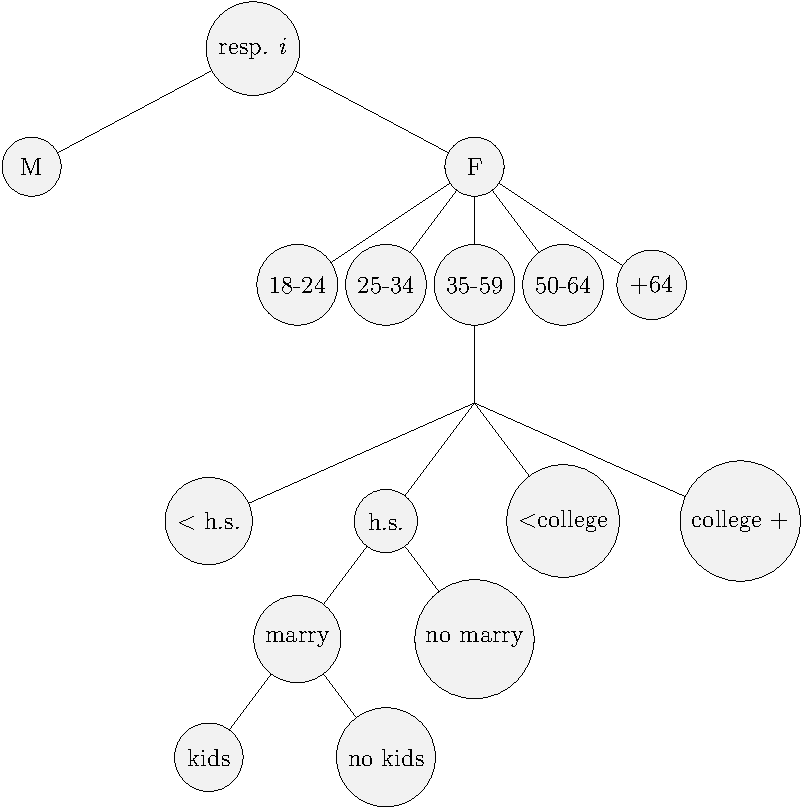
\includegraphics[height = \textwidth, width = \textwidth]{figs/GroupCat}
\end{figure}

Motivation for the instrument follows from the heterogeneity in inflation expectations across demographic groups.  While the diversity of Michigan survey expectations is well-known, the following summarizes the particular variation exploited by the current paper's research design.  The remainder of this section documents the demographic and expectational variation.

The Michigan survey records a variety of demographic factors as well as the consumer's Census region. A panel of demographic groups follows the categorization of each of the roughly 273,000 survey responses, from 1978.1-2022.5, into one of 160 categories based on sex, age, education, marital and parental status. Those categories shown in Figure \ref{fig:GroupTree}, produce a panel that consists of $T = 528$ months, $N = 4$ regions, and $G=160$ groups. For each group, the vector of controls includes, among other variables, additional survey questions about consumer perceptions of the economy, unemployment, personal income, expected future income, gas price expectations, current consumer financial status, and expected household financial status. For each period, each region, and each group, the average inflation expectation is treated as the unit of observation.\footnote{The panel dimensions fit a ``small $N$, big $T$'' setting that raises potential finite sample bias concerns that the estimation will address.}

\begin{figure}
\centering
\caption{Group mean price expectations. Groups: men $\leq 80$, women $>80$. Each marker is particular group's sample average inflation expectations.  There is evident expectational heterogeneity across groups.  For example, the highest average expectations are in groups of younger women with less than a high school degree.  While the lowest average expectation are older, more educated consumers.}\label{fig:GroupMeans}
% Created by tikzDevice version 0.12.3.1 on 2023-10-23 15:56:30
% !TEX encoding = UTF-8 Unicode
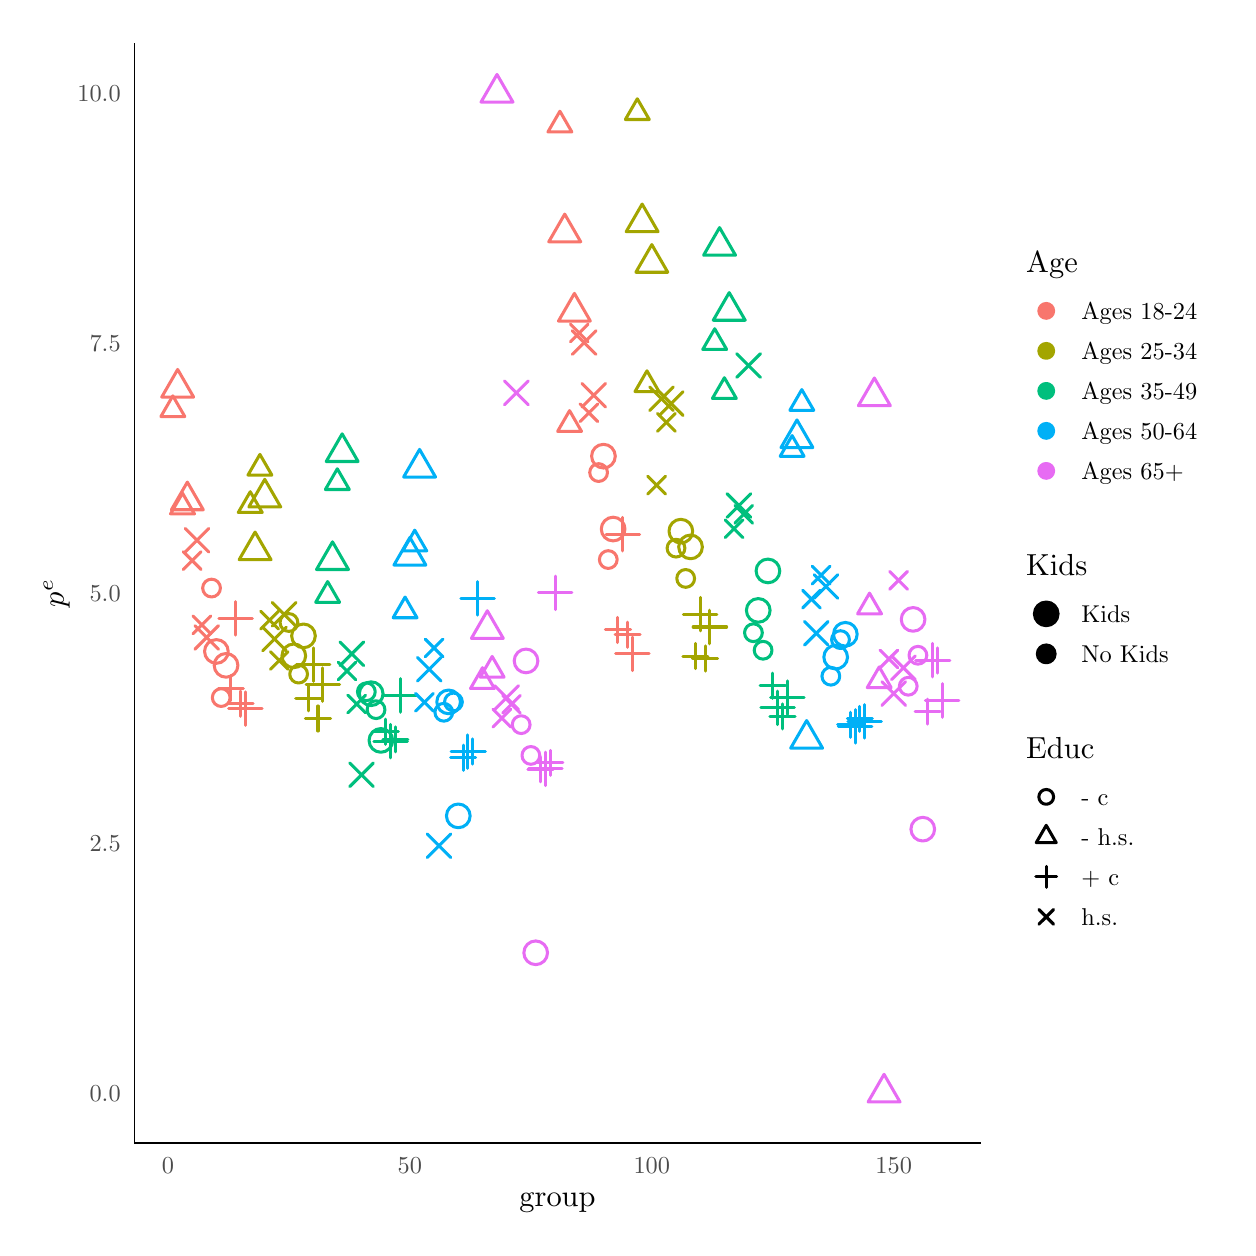
\begin{tikzpicture}[x=1pt,y=1pt]
\definecolor{fillColor}{RGB}{255,255,255}
\path[use as bounding box,fill=fillColor,fill opacity=0.00] (0,0) rectangle (433.62,433.62);
\begin{scope}
\path[clip] ( 38.56, 30.69) rectangle (344.33,428.12);
\definecolor{drawColor}{RGB}{248,118,109}

\path[draw=drawColor,line width= 1.1pt,line join=round,line cap=round] ( 52.45,300.57) --
	( 56.78,293.09) --
	( 48.13,293.09) --
	cycle;

\path[draw=drawColor,line width= 1.1pt,line join=round,line cap=round] ( 54.20,310.11) --
	( 59.97,300.13) --
	( 48.44,300.13) --
	cycle;

\path[draw=drawColor,line width= 1.1pt,line join=round,line cap=round] ( 55.95,265.41) --
	( 60.27,257.92) --
	( 51.63,257.92) --
	cycle;

\path[draw=drawColor,line width= 1.1pt,line join=round,line cap=round] ( 57.70,269.40) --
	( 63.46,259.41) --
	( 51.93,259.41) --
	cycle;

\path[draw=drawColor,line width= 1.1pt,line join=round,line cap=round] ( 56.24,237.85) -- ( 62.66,244.27);

\path[draw=drawColor,line width= 1.1pt,line join=round,line cap=round] ( 56.24,244.27) -- ( 62.66,237.85);

\path[draw=drawColor,line width= 1.1pt,line join=round,line cap=round] ( 56.92,244.13) -- ( 65.48,252.69);

\path[draw=drawColor,line width= 1.1pt,line join=round,line cap=round] ( 56.92,252.69) -- ( 65.48,244.13);

\path[draw=drawColor,line width= 1.1pt,line join=round,line cap=round] ( 59.73,214.58) -- ( 66.15,221.00);

\path[draw=drawColor,line width= 1.1pt,line join=round,line cap=round] ( 59.73,221.00) -- ( 66.15,214.58);

\path[draw=drawColor,line width= 1.1pt,line join=round,line cap=round] ( 60.41,209.00) -- ( 68.97,217.56);

\path[draw=drawColor,line width= 1.1pt,line join=round,line cap=round] ( 60.41,217.56) -- ( 68.97,209.00);

\path[draw=drawColor,line width= 1.1pt,line join=round,line cap=round] ( 66.44,231.12) circle (  3.21);

\path[draw=drawColor,line width= 1.1pt,line join=round,line cap=round] ( 68.19,208.22) circle (  4.28);

\path[draw=drawColor,line width= 1.1pt,line join=round,line cap=round] ( 69.94,191.55) circle (  3.21);

\path[draw=drawColor,line width= 1.1pt,line join=round,line cap=round] ( 71.68,203.19) circle (  4.28);

\path[draw=drawColor,line width= 1.1pt,line join=round,line cap=round] ( 68.89,194.94) -- ( 77.97,194.94);

\path[draw=drawColor,line width= 1.1pt,line join=round,line cap=round] ( 73.43,190.40) -- ( 73.43,199.48);

\path[draw=drawColor,line width= 1.1pt,line join=round,line cap=round] ( 69.13,220.20) -- ( 81.23,220.20);

\path[draw=drawColor,line width= 1.1pt,line join=round,line cap=round] ( 75.18,214.15) -- ( 75.18,226.25);

\path[draw=drawColor,line width= 1.1pt,line join=round,line cap=round] ( 72.39,189.34) -- ( 81.47,189.34);

\path[draw=drawColor,line width= 1.1pt,line join=round,line cap=round] ( 76.93,184.80) -- ( 76.93,193.88);

\path[draw=drawColor,line width= 1.1pt,line join=round,line cap=round] ( 72.63,187.56) -- ( 84.73,187.56);

\path[draw=drawColor,line width= 1.1pt,line join=round,line cap=round] ( 78.68,181.50) -- ( 78.68,193.61);
\definecolor{drawColor}{RGB}{163,165,0}

\path[draw=drawColor,line width= 1.1pt,line join=round,line cap=round] ( 80.43,265.93) --
	( 84.75,258.44) --
	( 76.10,258.44) --
	cycle;

\path[draw=drawColor,line width= 1.1pt,line join=round,line cap=round] ( 82.17,251.35) --
	( 87.94,241.37) --
	( 76.41,241.37) --
	cycle;

\path[draw=drawColor,line width= 1.1pt,line join=round,line cap=round] ( 83.92,279.42) --
	( 88.24,271.94) --
	( 79.60,271.94) --
	cycle;

\path[draw=drawColor,line width= 1.1pt,line join=round,line cap=round] ( 85.67,270.41) --
	( 91.43,260.43) --
	( 79.91,260.43) --
	cycle;

\path[draw=drawColor,line width= 1.1pt,line join=round,line cap=round] ( 84.21,216.33) -- ( 90.63,222.75);

\path[draw=drawColor,line width= 1.1pt,line join=round,line cap=round] ( 84.21,222.75) -- ( 90.63,216.33);

\path[draw=drawColor,line width= 1.1pt,line join=round,line cap=round] ( 84.89,208.45) -- ( 93.45,217.01);

\path[draw=drawColor,line width= 1.1pt,line join=round,line cap=round] ( 84.89,217.01) -- ( 93.45,208.45);

\path[draw=drawColor,line width= 1.1pt,line join=round,line cap=round] ( 87.71,201.74) -- ( 94.12,208.15);

\path[draw=drawColor,line width= 1.1pt,line join=round,line cap=round] ( 87.71,208.15) -- ( 94.12,201.74);

\path[draw=drawColor,line width= 1.1pt,line join=round,line cap=round] ( 88.38,217.36) -- ( 96.94,225.92);

\path[draw=drawColor,line width= 1.1pt,line join=round,line cap=round] ( 88.38,225.92) -- ( 96.94,217.36);

\path[draw=drawColor,line width= 1.1pt,line join=round,line cap=round] ( 94.41,218.67) circle (  3.21);

\path[draw=drawColor,line width= 1.1pt,line join=round,line cap=round] ( 96.16,206.63) circle (  4.28);

\path[draw=drawColor,line width= 1.1pt,line join=round,line cap=round] ( 97.91,200.03) circle (  3.21);

\path[draw=drawColor,line width= 1.1pt,line join=round,line cap=round] ( 99.66,213.84) circle (  4.28);

\path[draw=drawColor,line width= 1.1pt,line join=round,line cap=round] ( 96.87,191.24) -- (105.94,191.24);

\path[draw=drawColor,line width= 1.1pt,line join=round,line cap=round] (101.41,186.71) -- (101.41,195.78);

\path[draw=drawColor,line width= 1.1pt,line join=round,line cap=round] ( 97.10,203.45) -- (109.21,203.45);

\path[draw=drawColor,line width= 1.1pt,line join=round,line cap=round] (103.15,197.40) -- (103.15,209.50);

\path[draw=drawColor,line width= 1.1pt,line join=round,line cap=round] (100.36,183.98) -- (109.44,183.98);

\path[draw=drawColor,line width= 1.1pt,line join=round,line cap=round] (104.90,179.45) -- (104.90,188.52);

\path[draw=drawColor,line width= 1.1pt,line join=round,line cap=round] (100.60,196.22) -- (112.70,196.22);

\path[draw=drawColor,line width= 1.1pt,line join=round,line cap=round] (106.65,190.17) -- (106.65,202.27);
\definecolor{drawColor}{RGB}{0,191,125}

\path[draw=drawColor,line width= 1.1pt,line join=round,line cap=round] (108.40,233.46) --
	(112.72,225.97) --
	(104.08,225.97) --
	cycle;

\path[draw=drawColor,line width= 1.1pt,line join=round,line cap=round] (110.15,247.82) --
	(115.91,237.83) --
	(104.38,237.83) --
	cycle;

\path[draw=drawColor,line width= 1.1pt,line join=round,line cap=round] (111.89,274.22) --
	(116.22,266.73) --
	(107.57,266.73) --
	cycle;

\path[draw=drawColor,line width= 1.1pt,line join=round,line cap=round] (113.64,286.84) --
	(119.41,276.85) --
	(107.88,276.85) --
	cycle;

\path[draw=drawColor,line width= 1.1pt,line join=round,line cap=round] (112.18,197.95) -- (118.60,204.37);

\path[draw=drawColor,line width= 1.1pt,line join=round,line cap=round] (112.18,204.37) -- (118.60,197.95);

\path[draw=drawColor,line width= 1.1pt,line join=round,line cap=round] (112.86,203.09) -- (121.42,211.65);

\path[draw=drawColor,line width= 1.1pt,line join=round,line cap=round] (112.86,211.65) -- (121.42,203.09);

\path[draw=drawColor,line width= 1.1pt,line join=round,line cap=round] (115.68,186.02) -- (122.10,192.44);

\path[draw=drawColor,line width= 1.1pt,line join=round,line cap=round] (115.68,192.44) -- (122.10,186.02);

\path[draw=drawColor,line width= 1.1pt,line join=round,line cap=round] (116.36,159.36) -- (124.92,167.92);

\path[draw=drawColor,line width= 1.1pt,line join=round,line cap=round] (116.36,167.92) -- (124.92,159.36);

\path[draw=drawColor,line width= 1.1pt,line join=round,line cap=round] (122.38,193.64) circle (  3.21);

\path[draw=drawColor,line width= 1.1pt,line join=round,line cap=round] (124.13,192.95) circle (  4.28);

\path[draw=drawColor,line width= 1.1pt,line join=round,line cap=round] (125.88,187.18) circle (  3.21);

\path[draw=drawColor,line width= 1.1pt,line join=round,line cap=round] (127.63,176.07) circle (  4.28);

\path[draw=drawColor,line width= 1.1pt,line join=round,line cap=round] (124.84,179.18) -- (133.92,179.18);

\path[draw=drawColor,line width= 1.1pt,line join=round,line cap=round] (129.38,174.64) -- (129.38,183.72);

\path[draw=drawColor,line width= 1.1pt,line join=round,line cap=round] (125.07,175.84) -- (137.18,175.84);

\path[draw=drawColor,line width= 1.1pt,line join=round,line cap=round] (131.13,169.79) -- (131.13,181.89);

\path[draw=drawColor,line width= 1.1pt,line join=round,line cap=round] (128.34,176.45) -- (137.41,176.45);

\path[draw=drawColor,line width= 1.1pt,line join=round,line cap=round] (132.87,171.91) -- (132.87,180.99);

\path[draw=drawColor,line width= 1.1pt,line join=round,line cap=round] (128.57,192.30) -- (140.68,192.30);

\path[draw=drawColor,line width= 1.1pt,line join=round,line cap=round] (134.62,186.25) -- (134.62,198.36);
\definecolor{drawColor}{RGB}{0,176,246}

\path[draw=drawColor,line width= 1.1pt,line join=round,line cap=round] (136.37,227.87) --
	(140.69,220.39) --
	(132.05,220.39) --
	cycle;

\path[draw=drawColor,line width= 1.1pt,line join=round,line cap=round] (138.12,249.41) --
	(143.88,239.43) --
	(132.35,239.43) --
	cycle;

\path[draw=drawColor,line width= 1.1pt,line join=round,line cap=round] (139.87,252.04) --
	(144.19,244.55) --
	(135.55,244.55) --
	cycle;

\path[draw=drawColor,line width= 1.1pt,line join=round,line cap=round] (141.62,281.22) --
	(147.38,271.24) --
	(135.85,271.24) --
	cycle;

\path[draw=drawColor,line width= 1.1pt,line join=round,line cap=round] (140.15,186.65) -- (146.57,193.06);

\path[draw=drawColor,line width= 1.1pt,line join=round,line cap=round] (140.15,193.06) -- (146.57,186.65);

\path[draw=drawColor,line width= 1.1pt,line join=round,line cap=round] (140.83,197.53) -- (149.39,206.09);

\path[draw=drawColor,line width= 1.1pt,line join=round,line cap=round] (140.83,206.09) -- (149.39,197.53);

\path[draw=drawColor,line width= 1.1pt,line join=round,line cap=round] (143.65,206.26) -- (150.07,212.68);

\path[draw=drawColor,line width= 1.1pt,line join=round,line cap=round] (143.65,212.68) -- (150.07,206.26);

\path[draw=drawColor,line width= 1.1pt,line join=round,line cap=round] (144.33,133.73) -- (152.89,142.29);

\path[draw=drawColor,line width= 1.1pt,line join=round,line cap=round] (144.33,142.29) -- (152.89,133.73);

\path[draw=drawColor,line width= 1.1pt,line join=round,line cap=round] (150.36,186.24) circle (  3.21);

\path[draw=drawColor,line width= 1.1pt,line join=round,line cap=round] (152.11,189.99) circle (  4.28);

\path[draw=drawColor,line width= 1.1pt,line join=round,line cap=round] (153.85,189.97) circle (  3.21);

\path[draw=drawColor,line width= 1.1pt,line join=round,line cap=round] (155.60,148.80) circle (  4.28);

\path[draw=drawColor,line width= 1.1pt,line join=round,line cap=round] (152.81,169.81) -- (161.89,169.81);

\path[draw=drawColor,line width= 1.1pt,line join=round,line cap=round] (157.35,165.27) -- (157.35,174.35);

\path[draw=drawColor,line width= 1.1pt,line join=round,line cap=round] (153.05,172.03) -- (165.15,172.03);

\path[draw=drawColor,line width= 1.1pt,line join=round,line cap=round] (159.10,165.98) -- (159.10,178.08);

\path[draw=drawColor,line width= 1.1pt,line join=round,line cap=round] (156.31,172.06) -- (165.38,172.06);

\path[draw=drawColor,line width= 1.1pt,line join=round,line cap=round] (160.85,167.52) -- (160.85,176.59);

\path[draw=drawColor,line width= 1.1pt,line join=round,line cap=round] (156.54,227.40) -- (168.65,227.40);

\path[draw=drawColor,line width= 1.1pt,line join=round,line cap=round] (162.59,221.34) -- (162.59,233.45);
\definecolor{drawColor}{RGB}{231,107,243}

\path[draw=drawColor,line width= 1.1pt,line join=round,line cap=round] (164.34,202.33) --
	(168.66,194.84) --
	(160.02,194.84) --
	cycle;

\path[draw=drawColor,line width= 1.1pt,line join=round,line cap=round] (166.09,222.92) --
	(171.86,212.94) --
	(160.33,212.94) --
	cycle;

\path[draw=drawColor,line width= 1.1pt,line join=round,line cap=round] (167.84,206.41) --
	(172.16,198.93) --
	(163.52,198.93) --
	cycle;

\path[draw=drawColor,line width= 1.1pt,line join=round,line cap=round] (169.59,416.71) --
	(175.35,406.73) --
	(163.82,406.73) --
	cycle;

\path[draw=drawColor,line width= 1.1pt,line join=round,line cap=round] (168.13,180.90) -- (174.54,187.31);

\path[draw=drawColor,line width= 1.1pt,line join=round,line cap=round] (168.13,187.31) -- (174.54,180.90);

\path[draw=drawColor,line width= 1.1pt,line join=round,line cap=round] (168.80,187.26) -- (177.36,195.82);

\path[draw=drawColor,line width= 1.1pt,line join=round,line cap=round] (168.80,195.82) -- (177.36,187.26);

\path[draw=drawColor,line width= 1.1pt,line join=round,line cap=round] (171.62,185.94) -- (178.04,192.36);

\path[draw=drawColor,line width= 1.1pt,line join=round,line cap=round] (171.62,192.36) -- (178.04,185.94);

\path[draw=drawColor,line width= 1.1pt,line join=round,line cap=round] (172.30,297.38) -- (180.86,305.94);

\path[draw=drawColor,line width= 1.1pt,line join=round,line cap=round] (172.30,305.94) -- (180.86,297.38);

\path[draw=drawColor,line width= 1.1pt,line join=round,line cap=round] (178.33,181.77) circle (  3.21);

\path[draw=drawColor,line width= 1.1pt,line join=round,line cap=round] (180.08,204.79) circle (  4.28);

\path[draw=drawColor,line width= 1.1pt,line join=round,line cap=round] (181.83,170.64) circle (  3.21);

\path[draw=drawColor,line width= 1.1pt,line join=round,line cap=round] (183.57, 99.33) circle (  4.28);

\path[draw=drawColor,line width= 1.1pt,line join=round,line cap=round] (180.78,165.59) -- (189.86,165.59);

\path[draw=drawColor,line width= 1.1pt,line join=round,line cap=round] (185.32,161.05) -- (185.32,170.13);

\path[draw=drawColor,line width= 1.1pt,line join=round,line cap=round] (181.02,165.78) -- (193.12,165.78);

\path[draw=drawColor,line width= 1.1pt,line join=round,line cap=round] (187.07,159.73) -- (187.07,171.83);

\path[draw=drawColor,line width= 1.1pt,line join=round,line cap=round] (184.28,167.94) -- (193.36,167.94);

\path[draw=drawColor,line width= 1.1pt,line join=round,line cap=round] (188.82,163.40) -- (188.82,172.48);

\path[draw=drawColor,line width= 1.1pt,line join=round,line cap=round] (184.51,229.40) -- (196.62,229.40);

\path[draw=drawColor,line width= 1.1pt,line join=round,line cap=round] (190.57,223.35) -- (190.57,235.46);
\definecolor{drawColor}{RGB}{248,118,109}

\path[draw=drawColor,line width= 1.1pt,line join=round,line cap=round] (192.32,403.42) --
	(196.64,395.93) --
	(187.99,395.93) --
	cycle;

\path[draw=drawColor,line width= 1.1pt,line join=round,line cap=round] (194.06,366.24) --
	(199.83,356.25) --
	(188.30,356.25) --
	cycle;

\path[draw=drawColor,line width= 1.1pt,line join=round,line cap=round] (195.81,295.23) --
	(200.13,287.74) --
	(191.49,287.74) --
	cycle;

\path[draw=drawColor,line width= 1.1pt,line join=round,line cap=round] (197.56,337.59) --
	(203.32,327.60) --
	(191.80,327.60) --
	cycle;

\path[draw=drawColor,line width= 1.1pt,line join=round,line cap=round] (196.10,320.10) -- (202.52,326.52);

\path[draw=drawColor,line width= 1.1pt,line join=round,line cap=round] (196.10,326.52) -- (202.52,320.10);

\path[draw=drawColor,line width= 1.1pt,line join=round,line cap=round] (196.78,315.55) -- (205.34,324.11);

\path[draw=drawColor,line width= 1.1pt,line join=round,line cap=round] (196.78,324.11) -- (205.34,315.55);

\path[draw=drawColor,line width= 1.1pt,line join=round,line cap=round] (199.60,291.25) -- (206.01,297.67);

\path[draw=drawColor,line width= 1.1pt,line join=round,line cap=round] (199.60,297.67) -- (206.01,291.25);

\path[draw=drawColor,line width= 1.1pt,line join=round,line cap=round] (200.27,296.54) -- (208.83,305.10);

\path[draw=drawColor,line width= 1.1pt,line join=round,line cap=round] (200.27,305.10) -- (208.83,296.54);

\path[draw=drawColor,line width= 1.1pt,line join=round,line cap=round] (206.30,272.86) circle (  3.21);

\path[draw=drawColor,line width= 1.1pt,line join=round,line cap=round] (208.05,278.78) circle (  4.28);

\path[draw=drawColor,line width= 1.1pt,line join=round,line cap=round] (209.80,241.42) circle (  3.21);

\path[draw=drawColor,line width= 1.1pt,line join=round,line cap=round] (211.55,252.44) circle (  4.28);

\path[draw=drawColor,line width= 1.1pt,line join=round,line cap=round] (208.76,215.98) -- (217.83,215.98);

\path[draw=drawColor,line width= 1.1pt,line join=round,line cap=round] (213.29,211.45) -- (213.29,220.52);

\path[draw=drawColor,line width= 1.1pt,line join=round,line cap=round] (208.99,250.58) -- (221.10,250.58);

\path[draw=drawColor,line width= 1.1pt,line join=round,line cap=round] (215.04,244.52) -- (215.04,256.63);

\path[draw=drawColor,line width= 1.1pt,line join=round,line cap=round] (212.25,214.26) -- (221.33,214.26);

\path[draw=drawColor,line width= 1.1pt,line join=round,line cap=round] (216.79,209.73) -- (216.79,218.80);

\path[draw=drawColor,line width= 1.1pt,line join=round,line cap=round] (212.49,207.36) -- (224.59,207.36);

\path[draw=drawColor,line width= 1.1pt,line join=round,line cap=round] (218.54,201.30) -- (218.54,213.41);
\definecolor{drawColor}{RGB}{163,165,0}

\path[draw=drawColor,line width= 1.1pt,line join=round,line cap=round] (220.29,407.92) --
	(224.61,400.43) --
	(215.97,400.43) --
	cycle;

\path[draw=drawColor,line width= 1.1pt,line join=round,line cap=round] (222.04,369.88) --
	(227.80,359.90) --
	(216.27,359.90) --
	cycle;

\path[draw=drawColor,line width= 1.1pt,line join=round,line cap=round] (223.78,309.62) --
	(228.11,302.13) --
	(219.46,302.13) --
	cycle;

\path[draw=drawColor,line width= 1.1pt,line join=round,line cap=round] (225.53,355.22) --
	(231.30,345.24) --
	(219.77,345.24) --
	cycle;

\path[draw=drawColor,line width= 1.1pt,line join=round,line cap=round] (224.07,265.10) -- (230.49,271.52);

\path[draw=drawColor,line width= 1.1pt,line join=round,line cap=round] (224.07,271.52) -- (230.49,265.10);

\path[draw=drawColor,line width= 1.1pt,line join=round,line cap=round] (224.75,295.22) -- (233.31,303.78);

\path[draw=drawColor,line width= 1.1pt,line join=round,line cap=round] (224.75,303.78) -- (233.31,295.22);

\path[draw=drawColor,line width= 1.1pt,line join=round,line cap=round] (227.57,287.76) -- (233.99,294.18);

\path[draw=drawColor,line width= 1.1pt,line join=round,line cap=round] (227.57,294.18) -- (233.99,287.76);

\path[draw=drawColor,line width= 1.1pt,line join=round,line cap=round] (228.25,293.50) -- (236.81,302.06);

\path[draw=drawColor,line width= 1.1pt,line join=round,line cap=round] (228.25,302.06) -- (236.81,293.50);

\path[draw=drawColor,line width= 1.1pt,line join=round,line cap=round] (234.27,245.54) circle (  3.21);

\path[draw=drawColor,line width= 1.1pt,line join=round,line cap=round] (236.02,251.68) circle (  4.28);

\path[draw=drawColor,line width= 1.1pt,line join=round,line cap=round] (237.77,234.60) circle (  3.21);

\path[draw=drawColor,line width= 1.1pt,line join=round,line cap=round] (239.52,245.99) circle (  4.28);

\path[draw=drawColor,line width= 1.1pt,line join=round,line cap=round] (236.73,206.56) -- (245.80,206.56);

\path[draw=drawColor,line width= 1.1pt,line join=round,line cap=round] (241.27,202.02) -- (241.27,211.10);

\path[draw=drawColor,line width= 1.1pt,line join=round,line cap=round] (236.96,221.72) -- (249.07,221.72);

\path[draw=drawColor,line width= 1.1pt,line join=round,line cap=round] (243.01,215.66) -- (243.01,227.77);

\path[draw=drawColor,line width= 1.1pt,line join=round,line cap=round] (240.23,205.65) -- (249.30,205.65);

\path[draw=drawColor,line width= 1.1pt,line join=round,line cap=round] (244.76,201.11) -- (244.76,210.19);

\path[draw=drawColor,line width= 1.1pt,line join=round,line cap=round] (240.46,217.05) -- (252.56,217.05);

\path[draw=drawColor,line width= 1.1pt,line join=round,line cap=round] (246.51,211.00) -- (246.51,223.10);
\definecolor{drawColor}{RGB}{0,191,125}

\path[draw=drawColor,line width= 1.1pt,line join=round,line cap=round] (248.26,324.82) --
	(252.58,317.34) --
	(243.94,317.34) --
	cycle;

\path[draw=drawColor,line width= 1.1pt,line join=round,line cap=round] (250.01,361.37) --
	(255.77,351.39) --
	(244.24,351.39) --
	cycle;

\path[draw=drawColor,line width= 1.1pt,line join=round,line cap=round] (251.76,307.12) --
	(256.08,299.64) --
	(247.43,299.64) --
	cycle;

\path[draw=drawColor,line width= 1.1pt,line join=round,line cap=round] (253.50,337.88) --
	(259.27,327.90) --
	(247.74,327.90) --
	cycle;

\path[draw=drawColor,line width= 1.1pt,line join=round,line cap=round] (252.04,249.33) -- (258.46,255.75);

\path[draw=drawColor,line width= 1.1pt,line join=round,line cap=round] (252.04,255.75) -- (258.46,249.33);

\path[draw=drawColor,line width= 1.1pt,line join=round,line cap=round] (252.72,256.67) -- (261.28,265.23);

\path[draw=drawColor,line width= 1.1pt,line join=round,line cap=round] (252.72,265.23) -- (261.28,256.67);

\path[draw=drawColor,line width= 1.1pt,line join=round,line cap=round] (255.54,254.56) -- (261.96,260.98);

\path[draw=drawColor,line width= 1.1pt,line join=round,line cap=round] (255.54,260.98) -- (261.96,254.56);

\path[draw=drawColor,line width= 1.1pt,line join=round,line cap=round] (256.22,307.25) -- (264.78,315.81);

\path[draw=drawColor,line width= 1.1pt,line join=round,line cap=round] (256.22,315.81) -- (264.78,307.25);

\path[draw=drawColor,line width= 1.1pt,line join=round,line cap=round] (262.25,214.98) circle (  3.21);

\path[draw=drawColor,line width= 1.1pt,line join=round,line cap=round] (263.99,223.05) circle (  4.28);

\path[draw=drawColor,line width= 1.1pt,line join=round,line cap=round] (265.74,208.65) circle (  3.21);

\path[draw=drawColor,line width= 1.1pt,line join=round,line cap=round] (267.49,237.31) circle (  4.28);

\path[draw=drawColor,line width= 1.1pt,line join=round,line cap=round] (264.70,195.84) -- (273.78,195.84);

\path[draw=drawColor,line width= 1.1pt,line join=round,line cap=round] (269.24,191.30) -- (269.24,200.37);

\path[draw=drawColor,line width= 1.1pt,line join=round,line cap=round] (264.93,187.80) -- (277.04,187.80);

\path[draw=drawColor,line width= 1.1pt,line join=round,line cap=round] (270.99,181.75) -- (270.99,193.85);

\path[draw=drawColor,line width= 1.1pt,line join=round,line cap=round] (268.20,184.73) -- (277.27,184.73);

\path[draw=drawColor,line width= 1.1pt,line join=round,line cap=round] (272.74,180.20) -- (272.74,189.27);

\path[draw=drawColor,line width= 1.1pt,line join=round,line cap=round] (268.43,191.51) -- (280.54,191.51);

\path[draw=drawColor,line width= 1.1pt,line join=round,line cap=round] (274.48,185.45) -- (274.48,197.56);
\definecolor{drawColor}{RGB}{0,176,246}

\path[draw=drawColor,line width= 1.1pt,line join=round,line cap=round] (276.23,286.22) --
	(280.55,278.73) --
	(271.91,278.73) --
	cycle;

\path[draw=drawColor,line width= 1.1pt,line join=round,line cap=round] (277.98,291.87) --
	(283.74,281.89) --
	(272.22,281.89) --
	cycle;

\path[draw=drawColor,line width= 1.1pt,line join=round,line cap=round] (279.73,302.83) --
	(284.05,295.35) --
	(275.41,295.35) --
	cycle;

\path[draw=drawColor,line width= 1.1pt,line join=round,line cap=round] (281.48,183.25) --
	(287.24,173.27) --
	(275.71,173.27) --
	cycle;

\path[draw=drawColor,line width= 1.1pt,line join=round,line cap=round] (280.02,223.91) -- (286.43,230.33);

\path[draw=drawColor,line width= 1.1pt,line join=round,line cap=round] (280.02,230.33) -- (286.43,223.91);

\path[draw=drawColor,line width= 1.1pt,line join=round,line cap=round] (280.69,210.49) -- (289.25,219.04);

\path[draw=drawColor,line width= 1.1pt,line join=round,line cap=round] (280.69,219.04) -- (289.25,210.49);

\path[draw=drawColor,line width= 1.1pt,line join=round,line cap=round] (283.51,232.58) -- (289.93,239.00);

\path[draw=drawColor,line width= 1.1pt,line join=round,line cap=round] (283.51,239.00) -- (289.93,232.58);

\path[draw=drawColor,line width= 1.1pt,line join=round,line cap=round] (284.19,227.38) -- (292.75,235.94);

\path[draw=drawColor,line width= 1.1pt,line join=round,line cap=round] (284.19,235.94) -- (292.75,227.38);

\path[draw=drawColor,line width= 1.1pt,line join=round,line cap=round] (290.22,199.27) circle (  3.21);

\path[draw=drawColor,line width= 1.1pt,line join=round,line cap=round] (291.97,206.16) circle (  4.28);

\path[draw=drawColor,line width= 1.1pt,line join=round,line cap=round] (293.71,212.49) circle (  3.21);

\path[draw=drawColor,line width= 1.1pt,line join=round,line cap=round] (295.46,214.42) circle (  4.28);

\path[draw=drawColor,line width= 1.1pt,line join=round,line cap=round] (292.67,181.70) -- (301.75,181.70);

\path[draw=drawColor,line width= 1.1pt,line join=round,line cap=round] (297.21,177.16) -- (297.21,186.24);

\path[draw=drawColor,line width= 1.1pt,line join=round,line cap=round] (292.91,181.16) -- (305.01,181.16);

\path[draw=drawColor,line width= 1.1pt,line join=round,line cap=round] (298.96,175.11) -- (298.96,187.22);

\path[draw=drawColor,line width= 1.1pt,line join=round,line cap=round] (296.17,183.86) -- (305.25,183.86);

\path[draw=drawColor,line width= 1.1pt,line join=round,line cap=round] (300.71,179.33) -- (300.71,188.40);

\path[draw=drawColor,line width= 1.1pt,line join=round,line cap=round] (296.40,182.95) -- (308.51,182.95);

\path[draw=drawColor,line width= 1.1pt,line join=round,line cap=round] (302.46,176.90) -- (302.46,189.00);
\definecolor{drawColor}{RGB}{231,107,243}

\path[draw=drawColor,line width= 1.1pt,line join=round,line cap=round] (304.20,229.29) --
	(308.53,221.80) --
	(299.88,221.80) --
	cycle;

\path[draw=drawColor,line width= 1.1pt,line join=round,line cap=round] (305.95,307.02) --
	(311.72,297.03) --
	(300.19,297.03) --
	cycle;

\path[draw=drawColor,line width= 1.1pt,line join=round,line cap=round] (307.70,202.63) --
	(312.02,195.15) --
	(303.38,195.15) --
	cycle;

\path[draw=drawColor,line width= 1.1pt,line join=round,line cap=round] (309.45, 55.41) --
	(315.21, 45.42) --
	(303.69, 45.42) --
	cycle;

\path[draw=drawColor,line width= 1.1pt,line join=round,line cap=round] (307.99,202.29) -- (314.41,208.70);

\path[draw=drawColor,line width= 1.1pt,line join=round,line cap=round] (307.99,208.70) -- (314.41,202.29);

\path[draw=drawColor,line width= 1.1pt,line join=round,line cap=round] (308.67,188.71) -- (317.23,197.27);

\path[draw=drawColor,line width= 1.1pt,line join=round,line cap=round] (308.67,197.27) -- (317.23,188.71);

\path[draw=drawColor,line width= 1.1pt,line join=round,line cap=round] (311.49,230.71) -- (317.90,237.13);

\path[draw=drawColor,line width= 1.1pt,line join=round,line cap=round] (311.49,237.13) -- (317.90,230.71);

\path[draw=drawColor,line width= 1.1pt,line join=round,line cap=round] (312.16,198.03) -- (320.72,206.59);

\path[draw=drawColor,line width= 1.1pt,line join=round,line cap=round] (312.16,206.59) -- (320.72,198.03);

\path[draw=drawColor,line width= 1.1pt,line join=round,line cap=round] (318.19,195.64) circle (  3.21);

\path[draw=drawColor,line width= 1.1pt,line join=round,line cap=round] (319.94,219.80) circle (  4.28);

\path[draw=drawColor,line width= 1.1pt,line join=round,line cap=round] (321.69,206.84) circle (  3.21);

\path[draw=drawColor,line width= 1.1pt,line join=round,line cap=round] (323.44,144.00) circle (  4.28);

\path[draw=drawColor,line width= 1.1pt,line join=round,line cap=round] (320.65,186.47) -- (329.72,186.47);

\path[draw=drawColor,line width= 1.1pt,line join=round,line cap=round] (325.18,181.94) -- (325.18,191.01);

\path[draw=drawColor,line width= 1.1pt,line join=round,line cap=round] (320.88,205.04) -- (332.98,205.04);

\path[draw=drawColor,line width= 1.1pt,line join=round,line cap=round] (326.93,198.99) -- (326.93,211.09);

\path[draw=drawColor,line width= 1.1pt,line join=round,line cap=round] (324.14,204.94) -- (333.22,204.94);

\path[draw=drawColor,line width= 1.1pt,line join=round,line cap=round] (328.68,200.40) -- (328.68,209.48);

\path[draw=drawColor,line width= 1.1pt,line join=round,line cap=round] (324.38,190.49) -- (336.48,190.49);

\path[draw=drawColor,line width= 1.1pt,line join=round,line cap=round] (330.43,184.44) -- (330.43,196.55);
\end{scope}
\begin{scope}
\path[clip] (  0.00,  0.00) rectangle (433.62,433.62);
\definecolor{drawColor}{RGB}{0,0,0}

\path[draw=drawColor,line width= 0.6pt,line join=round] ( 38.56, 30.69) --
	( 38.56,428.12);
\end{scope}
\begin{scope}
\path[clip] (  0.00,  0.00) rectangle (433.62,433.62);
\definecolor{drawColor}{gray}{0.30}

\node[text=drawColor,anchor=base east,inner sep=0pt, outer sep=0pt, scale=  0.88] at ( 33.61, 45.72) {0.0};

\node[text=drawColor,anchor=base east,inner sep=0pt, outer sep=0pt, scale=  0.88] at ( 33.61,136.05) {2.5};

\node[text=drawColor,anchor=base east,inner sep=0pt, outer sep=0pt, scale=  0.88] at ( 33.61,226.37) {5.0};

\node[text=drawColor,anchor=base east,inner sep=0pt, outer sep=0pt, scale=  0.88] at ( 33.61,316.70) {7.5};

\node[text=drawColor,anchor=base east,inner sep=0pt, outer sep=0pt, scale=  0.88] at ( 33.61,407.02) {10.0};
\end{scope}
\begin{scope}
\path[clip] (  0.00,  0.00) rectangle (433.62,433.62);
\definecolor{drawColor}{RGB}{0,0,0}

\path[draw=drawColor,line width= 0.6pt,line join=round] ( 38.56, 30.69) --
	(344.33, 30.69);
\end{scope}
\begin{scope}
\path[clip] (  0.00,  0.00) rectangle (433.62,433.62);
\definecolor{drawColor}{gray}{0.30}

\node[text=drawColor,anchor=base,inner sep=0pt, outer sep=0pt, scale=  0.88] at ( 50.71, 19.68) {0};

\node[text=drawColor,anchor=base,inner sep=0pt, outer sep=0pt, scale=  0.88] at (138.12, 19.68) {50};

\node[text=drawColor,anchor=base,inner sep=0pt, outer sep=0pt, scale=  0.88] at (225.53, 19.68) {100};

\node[text=drawColor,anchor=base,inner sep=0pt, outer sep=0pt, scale=  0.88] at (312.95, 19.68) {150};
\end{scope}
\begin{scope}
\path[clip] (  0.00,  0.00) rectangle (433.62,433.62);
\definecolor{drawColor}{RGB}{0,0,0}

\node[text=drawColor,anchor=base,inner sep=0pt, outer sep=0pt, scale=  1.10] at (191.44,  7.64) {group};
\end{scope}
\begin{scope}
\path[clip] (  0.00,  0.00) rectangle (433.62,433.62);
\definecolor{drawColor}{RGB}{0,0,0}

\node[text=drawColor,rotate= 90.00,anchor=base,inner sep=0pt, outer sep=0pt, scale=  1.10] at ( 13.08,229.40) {$p^e$};
\end{scope}
\begin{scope}
\path[clip] (  0.00,  0.00) rectangle (433.62,433.62);
\definecolor{drawColor}{RGB}{0,0,0}

\node[text=drawColor,anchor=base west,inner sep=0pt, outer sep=0pt, scale=  1.10] at (360.83,345.08) {Age};
\end{scope}
\begin{scope}
\path[clip] (  0.00,  0.00) rectangle (433.62,433.62);
\definecolor{drawColor}{RGB}{248,118,109}
\definecolor{fillColor}{RGB}{248,118,109}

\path[draw=drawColor,line width= 1.1pt,line join=round,line cap=round,fill=fillColor] (368.05,331.28) circle (  2.67);
\end{scope}
\begin{scope}
\path[clip] (  0.00,  0.00) rectangle (433.62,433.62);
\definecolor{drawColor}{RGB}{163,165,0}
\definecolor{fillColor}{RGB}{163,165,0}

\path[draw=drawColor,line width= 1.1pt,line join=round,line cap=round,fill=fillColor] (368.05,316.83) circle (  2.67);
\end{scope}
\begin{scope}
\path[clip] (  0.00,  0.00) rectangle (433.62,433.62);
\definecolor{drawColor}{RGB}{0,191,125}
\definecolor{fillColor}{RGB}{0,191,125}

\path[draw=drawColor,line width= 1.1pt,line join=round,line cap=round,fill=fillColor] (368.05,302.37) circle (  2.67);
\end{scope}
\begin{scope}
\path[clip] (  0.00,  0.00) rectangle (433.62,433.62);
\definecolor{drawColor}{RGB}{0,176,246}
\definecolor{fillColor}{RGB}{0,176,246}

\path[draw=drawColor,line width= 1.1pt,line join=round,line cap=round,fill=fillColor] (368.05,287.92) circle (  2.67);
\end{scope}
\begin{scope}
\path[clip] (  0.00,  0.00) rectangle (433.62,433.62);
\definecolor{drawColor}{RGB}{231,107,243}
\definecolor{fillColor}{RGB}{231,107,243}

\path[draw=drawColor,line width= 1.1pt,line join=round,line cap=round,fill=fillColor] (368.05,273.46) circle (  2.67);
\end{scope}
\begin{scope}
\path[clip] (  0.00,  0.00) rectangle (433.62,433.62);
\definecolor{drawColor}{RGB}{0,0,0}

\node[text=drawColor,anchor=base west,inner sep=0pt, outer sep=0pt, scale=  0.88] at (380.78,328.25) {Ages 18-24};
\end{scope}
\begin{scope}
\path[clip] (  0.00,  0.00) rectangle (433.62,433.62);
\definecolor{drawColor}{RGB}{0,0,0}

\node[text=drawColor,anchor=base west,inner sep=0pt, outer sep=0pt, scale=  0.88] at (380.78,313.80) {Ages 25-34};
\end{scope}
\begin{scope}
\path[clip] (  0.00,  0.00) rectangle (433.62,433.62);
\definecolor{drawColor}{RGB}{0,0,0}

\node[text=drawColor,anchor=base west,inner sep=0pt, outer sep=0pt, scale=  0.88] at (380.78,299.34) {Ages 35-49};
\end{scope}
\begin{scope}
\path[clip] (  0.00,  0.00) rectangle (433.62,433.62);
\definecolor{drawColor}{RGB}{0,0,0}

\node[text=drawColor,anchor=base west,inner sep=0pt, outer sep=0pt, scale=  0.88] at (380.78,284.89) {Ages 50-64};
\end{scope}
\begin{scope}
\path[clip] (  0.00,  0.00) rectangle (433.62,433.62);
\definecolor{drawColor}{RGB}{0,0,0}

\node[text=drawColor,anchor=base west,inner sep=0pt, outer sep=0pt, scale=  0.88] at (380.78,270.43) {Ages 65+};
\end{scope}
\begin{scope}
\path[clip] (  0.00,  0.00) rectangle (433.62,433.62);
\definecolor{drawColor}{RGB}{0,0,0}

\node[text=drawColor,anchor=base west,inner sep=0pt, outer sep=0pt, scale=  1.10] at (360.83,235.59) {Kids};
\end{scope}
\begin{scope}
\path[clip] (  0.00,  0.00) rectangle (433.62,433.62);
\definecolor{drawColor}{RGB}{0,0,0}
\definecolor{fillColor}{RGB}{0,0,0}

\path[draw=drawColor,line width= 1.1pt,line join=round,line cap=round,fill=fillColor] (368.05,221.80) circle (  4.28);
\end{scope}
\begin{scope}
\path[clip] (  0.00,  0.00) rectangle (433.62,433.62);
\definecolor{drawColor}{RGB}{0,0,0}
\definecolor{fillColor}{RGB}{0,0,0}

\path[draw=drawColor,line width= 1.1pt,line join=round,line cap=round,fill=fillColor] (368.05,207.34) circle (  3.21);
\end{scope}
\begin{scope}
\path[clip] (  0.00,  0.00) rectangle (433.62,433.62);
\definecolor{drawColor}{RGB}{0,0,0}

\node[text=drawColor,anchor=base west,inner sep=0pt, outer sep=0pt, scale=  0.88] at (380.78,218.77) {Kids};
\end{scope}
\begin{scope}
\path[clip] (  0.00,  0.00) rectangle (433.62,433.62);
\definecolor{drawColor}{RGB}{0,0,0}

\node[text=drawColor,anchor=base west,inner sep=0pt, outer sep=0pt, scale=  0.88] at (380.78,204.31) {No Kids};
\end{scope}
\begin{scope}
\path[clip] (  0.00,  0.00) rectangle (433.62,433.62);
\definecolor{drawColor}{RGB}{0,0,0}

\node[text=drawColor,anchor=base west,inner sep=0pt, outer sep=0pt, scale=  1.10] at (360.83,169.47) {Educ};
\end{scope}
\begin{scope}
\path[clip] (  0.00,  0.00) rectangle (433.62,433.62);
\definecolor{drawColor}{RGB}{0,0,0}

\path[draw=drawColor,line width= 1.1pt,line join=round,line cap=round] (368.05,155.67) circle (  2.67);
\end{scope}
\begin{scope}
\path[clip] (  0.00,  0.00) rectangle (433.62,433.62);
\definecolor{drawColor}{RGB}{0,0,0}

\path[draw=drawColor,line width= 1.1pt,line join=round,line cap=round] (368.05,145.38) --
	(371.65,139.14) --
	(364.45,139.14) --
	cycle;
\end{scope}
\begin{scope}
\path[clip] (  0.00,  0.00) rectangle (433.62,433.62);
\definecolor{drawColor}{RGB}{0,0,0}

\path[draw=drawColor,line width= 1.1pt,line join=round,line cap=round] (364.27,126.77) -- (371.83,126.77);

\path[draw=drawColor,line width= 1.1pt,line join=round,line cap=round] (368.05,122.98) -- (368.05,130.55);
\end{scope}
\begin{scope}
\path[clip] (  0.00,  0.00) rectangle (433.62,433.62);
\definecolor{drawColor}{RGB}{0,0,0}

\path[draw=drawColor,line width= 1.1pt,line join=round,line cap=round] (365.38,109.64) -- (370.73,114.98);

\path[draw=drawColor,line width= 1.1pt,line join=round,line cap=round] (365.38,114.98) -- (370.73,109.64);
\end{scope}
\begin{scope}
\path[clip] (  0.00,  0.00) rectangle (433.62,433.62);
\definecolor{drawColor}{RGB}{0,0,0}

\node[text=drawColor,anchor=base west,inner sep=0pt, outer sep=0pt, scale=  0.88] at (380.78,152.64) {- c};
\end{scope}
\begin{scope}
\path[clip] (  0.00,  0.00) rectangle (433.62,433.62);
\definecolor{drawColor}{RGB}{0,0,0}

\node[text=drawColor,anchor=base west,inner sep=0pt, outer sep=0pt, scale=  0.88] at (380.78,138.19) {- h.s.};
\end{scope}
\begin{scope}
\path[clip] (  0.00,  0.00) rectangle (433.62,433.62);
\definecolor{drawColor}{RGB}{0,0,0}

\node[text=drawColor,anchor=base west,inner sep=0pt, outer sep=0pt, scale=  0.88] at (380.78,123.74) {+ c};
\end{scope}
\begin{scope}
\path[clip] (  0.00,  0.00) rectangle (433.62,433.62);
\definecolor{drawColor}{RGB}{0,0,0}

\node[text=drawColor,anchor=base west,inner sep=0pt, outer sep=0pt, scale=  0.88] at (380.78,109.28) {h.s.};
\end{scope}
\end{tikzpicture}

\end{figure}

Figure \ref{fig:GroupMeans} provides the first snapshot of the variation exploited by the quasi-experimental design. Each point represents a particular demographic group's mean inflation expectations, averaged across regions and time. Groups below 80 are men, and above are women. Each age group and education level has its color and shape, and women's higher average inflation expectations (c.f. \cite{BryanVenkatu}) are apparent. Markers are large to represent those groups with children. The figure also illustrates a clear pattern of heterogeneity across age and schooling.


\begin{figure}
\centering
\caption{Distribution of inflation survey expectations: by groups}\label{fig:intro2}
\begin{subfigure}[t]{0.75\textwidth}
%\centering
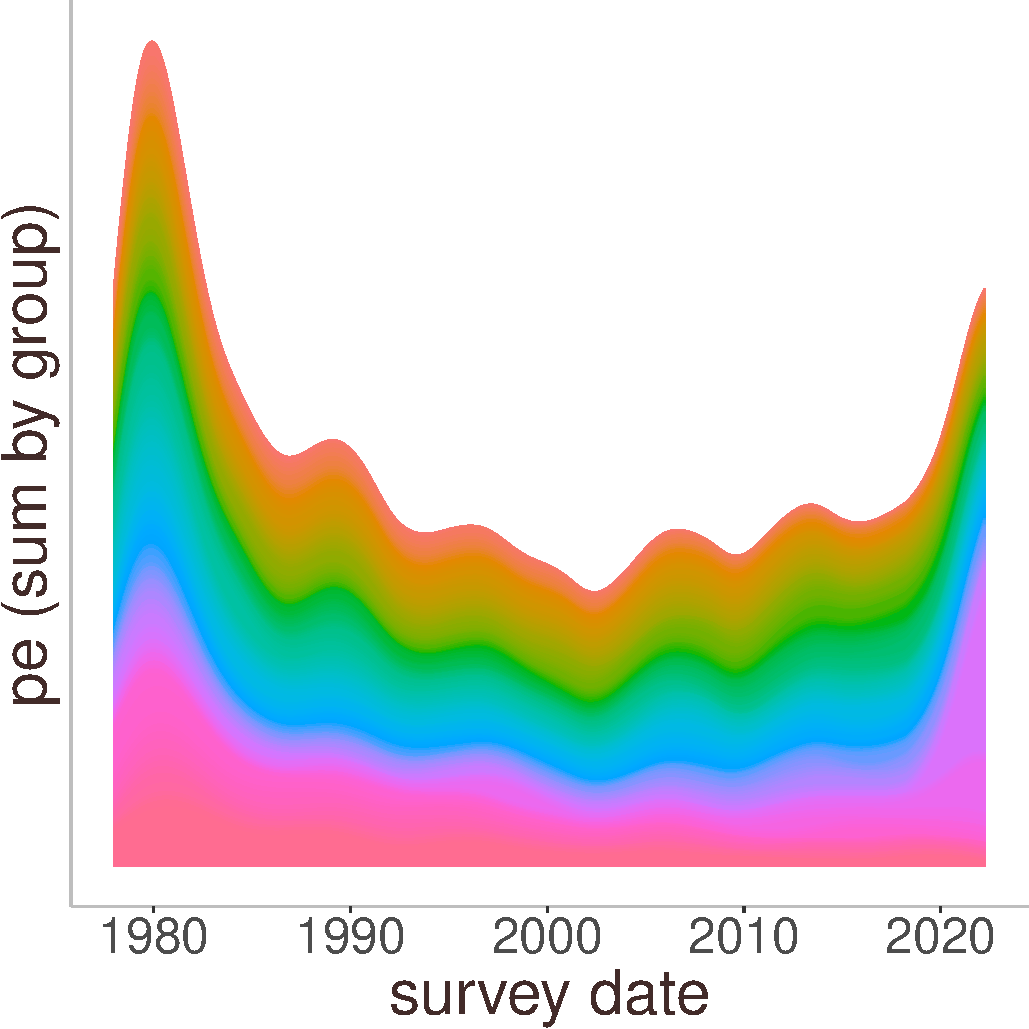
\includegraphics[width = 5in, height =3in]{figs/aggIndComp}
\caption{Inflation expectations $p^e$: all groups. Height = sum of expect.'s.}\label{fig:groupExpects}
\end{subfigure}
\vfill
\begin{subfigure}[t]{0.75\textwidth}
%\centering
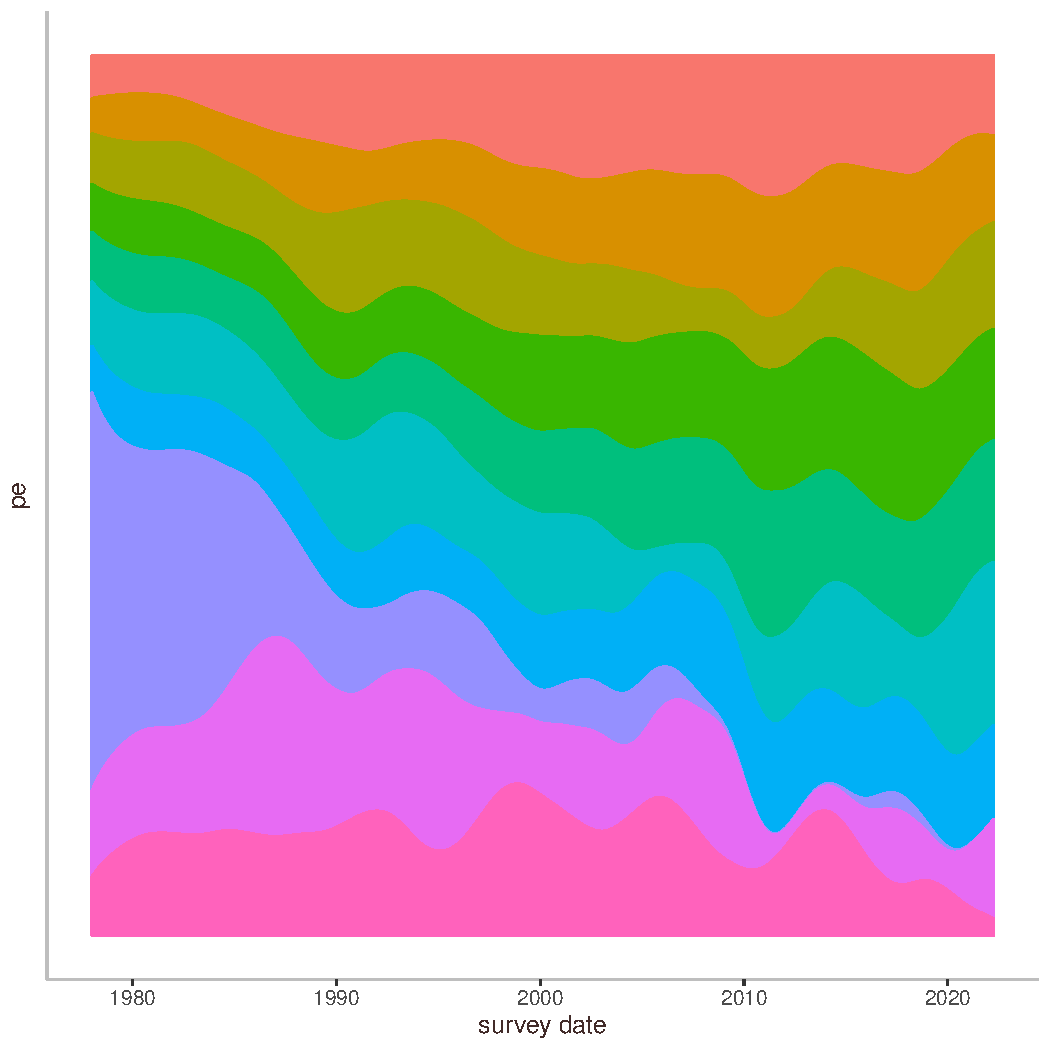
\includegraphics[width = 5in, height =3in]{figs/weightsTop10comp}
\caption{Inflation expectations $p^e$: key groups (unweighted avg.).}\label{fig:top10Expects}
\end{subfigure}
\end{figure}

Figure \ref{fig:intro2} provides a visual representation of the distribution of inflation expectations across groups.  This figure illustrates the aggregate variation in expectations exploited by the differential exposure design.  Each group is its own color gradient.  Panel \ref{fig:groupExpects} is the full distribution of aggregate inflation expectations.  The vertical axis in this panel is the sum of the expectations, $\sum_{g}\pi^e_{g,t}$.  The height of each group's section of the curve represents the average inflation expectation of that group during that moment in time.  The relative height, and share of the sum, for groups' expectations vary over time.  

Finally, panel \ref{fig:top10Expects} focuses on the ten groups that the empirical analysis identifies as particularly important and instead plots the proportional share of the (unweighted) average.  So, the height of each curve is that group's share of the total average inflation expectation.  Notice, for example, the lighter-blue group.  During the 1970s this group had the largest weight in the average inflation expectation.  By the mid-2000's the group is largely irrelevant.

\section{Empirical model}

\subsection{Motivating theory}

A standard model of Calvo pricing, extended to include multiple sectors, multiple groups of consumers, and subjective (possibly, non-rational) expectations, shows inflation to be a weighted average of each group's inflation expectation. A region is a closed economy consisting of a continuum of consumers and firms.\footnote{As motivation for the empirical model, the closed economy assumption is without a loss of generality, and the insights could extend to a currency union. \cite{NakamuraSteinsson:QJE2022} develop such a model and use regional variation to identify the slope of an aggregate Phillips curve under rational expectations.} The consumers can be classified into $G$ groups. There are $S$ sectors producing a differentiated consumption good. Each consumer decides on a lifetime consumption plan and a basket of goods. Consumer groups differ based on their preferences for bundles of consumption goods. Each group consumption basket is a time-invariant fraction of aggregate consumption. The production of consumption goods follows from a technology aggregating sector-specific intermediate goods produced by a continuum of monopolistically competitive firms with a linear production technology using labor as the only input. Intermediate producers in sector $s\in S$ face a Calvo risk that, with probability $1-\lambda_s$, the firm will be unable to adjust its price. The environment is standard with two exceptions: (1.) following \cite{Cravinoetal:JME2020} the extent of price stickiness can differ by sector, and (2.) rational expectations are not assumed.

As in \cite{Cravinoetal:JME2020}, there are multiple price indexes. There is the aggregate price index for consumer goods across sectors, $P_t$, as well as the consumer group $g\in G$ price index $P_t(g)$ that represents the cost of consuming group $g$'s bundle. Let $\theta$ denote the constant elasticity of substitution between goods. Group $g$'s price index is defined to be
$$ P_t(g) = \left( \sum_s \phi_s(g)P^{1-\theta}_{s,t}\right)^{1/(1-\theta)}$$
where $\phi_s(g)$ is a group-g specific preference parameter for consumption good $s$. The aggregate demand for consumption goods in sector $s$ is
$$ P_{s,t}C_{s,t} = \omega_{s,t}\left(\frac{P_{s,t}}{P_t}\right)^{1-\theta} P_tC_t$$
where $P_t=\left(\sum_s\omega_{s,t}P_{s,t}^{1-\theta}\right)^{1/(1-\theta)}$. The variable $\omega_{s,t}$ is the share of aggregate consumption in sector $s$. It is a weighted average across each consumer group's preference parameter $\phi_s(g)$, and the weights depend on the group's relative expenditure share. These weights are key to expressing the regional inflation rate in terms of the consumers' subjective inflation expectations.

Proceeding in the usual way, a firm producing intermediate goods in sector $s$, when allowed to reset prices in time $t$, optimally adjusts its (log) price according to
$$p^*_{s,t} - p_{s,t-1}= \left( 1-\beta\lambda_s\right)\sum_{T=t}^{\infty}\left(\beta\lambda_s\right)^{T-t}\left\{ \left(p^e_{s,T+1}-p_{s,t-1}\right) + w^e_{T}\right\}$$
where $(p^*)^e$ denotes a subjective expectation about own future prices, and $w_t$ is the marginal cost (real wage). Price-setting is forward-looking because the Calvo friction gives a probability $1-\lambda_s$ that prices remain fixed in the next period.  

Under rational expectations -- or any theory of expectation formation where subjective beliefs satisfy a law of iterated expectations -- the price-setting rule can be written recursively. However, a specific and simplified assumption on expectation formation is sufficient to motivate the empirical model. As in \cite{Woodford:annualreview}, individuals and firms are ``anticipated utility'' maximizers who may be adjusting (``learning'') their subjective expectations about inflation over time but assume for current decision-making that expected inflation would remain at its present rate. \cite{EvansHonkap-book} refer to this as ``steady-state learning.'' Letting the current inflation expectation, for sector $s$, be denoted as $\pi^e_s$, it follows that expectations about future prices evolve along a linear time trend, i.e. $p^e_{s,t+T} = (1+T)\pi^e_s$.\footnote{A similar simplifying assumption is made by \cite{Werning:expectsWP}.}. The inflation rate in sector $s$ is then
\begin{equation}\label{secPC}
 \pi_{s,t} = \left(1-\beta\lambda_s\right)^{-1} \pi^e_{s} + x_t
 \end{equation}
where $x_t$ is the expected present value of marginal cost factors.

Regional inflation is 
$$\pi^R_t = \sum_{s}\omega_{s,t}\pi_{s,t}$$
and group-specific inflation is
$$ \pi^g_t = \sum_s\omega^g_{s,t}\pi_{s,t}$$
Similarly, suppose that each group's subjective expectation for inflation is an expenditure-weighted average of expected inflation rates sector by sector. Let $\Pi^{e'}=\left(\pi^e(g)\right)_{g=1}^{G}, \Pi'_s=\left(\pi^e_s\right)_{s=1}^{S}, \Omega_s' = \left(\left(1-\beta\lambda_s\right)^{-1}\omega^g_s\right)_{s=1}^{S}$, and $\Omega' = \left(\Omega(g)\right)_g$. Then, and importantly, it is straightforward to recover firm expectations from consumer expectations.
\begin{equation}\label{Ident}
 \Pi^e = \Omega\Pi_s
\end{equation}
Plugging in for the sector-specific Phillips curves (\ref{secPC}) leads to
\begin{equation}\label{LOM}
\pi^R_t = \Omega_s'\Omega^{-1}\Pi^e_t + x_t
\end{equation}
The regional inflation rate is a weighted average of group-specific inflation rates and other factors that affect prices unrelated to inflation expectations. The weights depend on each sector's shares and the region's group-specific shares.

Similarly, it is possible to differentiate between short and long-run inflation expectations. Suppose that individuals forecast the one period ahead price as $p^e_{s,t+1} = \pi^e_t$ and then longer horizon expectations as before $p^e_{s,t+1+T} = (2+T)\bar{\pi}_s$, with $\bar{\pi}_s$ denoting the long-run inflation expectation for goods in sector $s$. Then
$$ \pi_t^R = \sum_s\omega_{s,t}\left( 1-\beta\lambda_s\right)\pi^e_{s,t+1}+\sum_s\omega_{s,t}\left[1+\left(1-\beta\lambda_s\right)^{-1}\right]\bar{\pi}_s + x_t$$
and so
$$ \pi_t^R = \hat{\Omega}_s'\Omega^{-1}\pi^e_t + \tilde{\Omega}_s'\Omega^{-1}\bar{\pi}+x_t$$
where $\hat{\Omega}'=\left(\omega_s(1-\beta\lambda)\right)_{s}, \tilde{\Omega}' = \left[ \omega_s\left( 1+(1-\beta\lambda )^{-1}\right)\right]$.

In conclusion,
\begin{itemize}
\item The inflation rate, at a regional level, depends positively on subjective inflation expectations.
\item Group expectations reflect the relative weight of expected inflation in each sector, with the weights capturing heterogeneity in consumption baskets.
\item The strength of the impact of expectations on inflation depends on the extent of price stickiness across sectors, consumer-group preferences for consumer goods in various sectors, and the distribution of consumers across the groups in a region.
\item Consumer-group expenditure shares depend on the \emph{level} of prices but not the rate of change, i.e., inflation.
\item Although a region is a closed economy, inflation could still depend on aggregate macroeconomic factors, particularly through $x_t$. 
\item Short and long-horizon expectations have different quantitative effects on regional inflation.
\item The empirical strategy exploits cross-sectional variation in sectoral demand to identify the effect inflation expectations have on prices.
\end{itemize}

\subsection{Mark ups and demographics}\label{subsec:markups}

The motivating model introduces consumption heterogeneity via idiosyncratic preference shocks, with expectations identified through the cross-group heterogeneity in consumption baskets. However, one potential issue that could challenge the exclusion restriction arises if different groups pay varied prices for identical goods. This disparity could occur if firms account for the different willingness to pay across diverse groups. In such a case, regional variations in mark-ups, as well as pass-through, might become endogenous to the group distribution.

Consider the following extension to \cite{AndersonRebeloWong:WP}. There exist $s=1,\ldots,S$ sectors, $g=1,\ldots,G$ groups, and a continuum $\left[0,n\right]$ of retail firms within each sector. While each firm sells the identical good, they offer a range of amenities (e.g., ease of parking, self-checkout), resulting in imperfect substitution among the firms' sectoral products. Let's denote $C_{s,g,t}$ as group $g$'s consumption of sector $s$'s goods, formulated as:
\begin{equation}
C_{s,g,t} = v_g^{\gamma}\left[\int_0^n x_{sigt}^{1/v_g}di\right]^{v_g}
\end{equation}
The elasticity of substitution across firms becomes:
\begin{equation}
-\frac{v_g}{1-v_g}
\end{equation}

A consumer of type $g$, in sector $s$, will face prices calculated as:
\begin{equation}
P_{sigt} = v^{\gamma/v_g}_gP_tC_{gt}^{v_g-1/v_g}x_{sigt}^{1-v_g/v_g}
\end{equation}
Consequently, the optimal price will have a constant mark-up $v_g$ above the marginal cost. Therefore, with group-specific elasticities of substitution across goods, it is conceivable that mark-ups and expectation pass-through could correlate with the distribution of groups across regions.

This concern, however, doesn't necessarily violate the exclusion restriction. The crucial point is that the group shares must not correlate with the inflation rate, rather than the price levels. An acyclical, or mostly time-invariant mark-up, would not pose an identification problem, as shown by \cite{AndersonRebeloWong:WP}. Nevertheless, we investigate this possibility in the data and find that mark-ups do not significantly correlate with group shares.

\subsection{Empirical model}

The object of interest is inflation expectations' impact on regional inflation rates. Expectations are endogenous. An instrument is constructed that exploits that demographic groups may have distinct preferences for the goods that make up a consumption basket. Their inflation expectations reflect the mix of prices in their basket. Interacting regional group shares with aggregate group inflation expectations instruments for the endogenous expectations. The empirical strategy is a differential exposure design: we identify the impact of expectations by measuring how a region's exposure to aggregate shocks leads to a differentiated inflation response. Each region has differential exposure to the shocks because of different population distributions. The identification strategy is valid so long as the demographic shares satisfy a relevance and an exogeneity condition.

The coefficient of interest is $\beta$ in the equation
\begin{equation}\label{OLS}
 \pi^R_t = \delta_R + \beta \pi^e_{R,t} + \kappa U_{R,t} + \gamma'x_{R,t} + \mu_t + \varepsilon_{R,t}
\end{equation}
where $\pi^R_t$ is the inflation rate in region $R$ at time $t$, $\pi^e_{R,t}$ is the expectation of 12-month ahead regional inflation, $U_{R,t}$ is the regional unemployment rate, $x_{R,t}$ is a vector of controls that includes lags of inflation, $\varepsilon_{R,t}$ is the structural disturbance, $\delta_R, \mu_t$ are region and time fixed effects, respectively. The endogeneity concern is that estimating (\ref{OLS}) via ordinary least squares will produce biased estimates of $\beta$ because $\pi^e_{R,t}$ is endogenous. In particular, endogeneity will arise if expectations respond, after controlling for exogenous covariates $x_{R,t}$, to the factors driving $\varepsilon_{R,t}$. While estimates of $\beta$ are not sensitive to bias from the endogeneity of unemployment, we follow \cite{NakamuraSteinsson:QJE2022} and instrument for $U_{R,t}$ using its 12-month lag.

A shift-share instrument (``Bartik instrument'') addresses the key endogeneity. Recall from (\ref{Ident}) that 
$$ \pi^e_{R,t} = \sum_{g}\omega_{R,g,t}\pi^e_{R,g,t}$$
Furthermore, if each region group's inflation expectation decomposes into aggregate and idiosyncratic components, then
$$ \pi^e_{R,g,t} = \pi^e_{g,t} + u_{R,g,t}$$
The empirical strategy uses exogenous variation in $\omega_{R,g,t}$ to generate differential exposure to the group-specific aggregate component $\pi^e_{g,t}$. The instrument is\footnote{The instruments are very closely related to inflation expectations. One concern is that, when calculating $\pi^e_{g,t}$, by averaging over all regions when computing the predicted inflation expectation in a region, the instrument is artificially very highly correlated with the region's inflation expectations. Accordingly, the paper reports results using a ``leave-one-out'' method so that $z_{RT}$ is computed by omitting the region's inflation expectations.}
$$ z_{R,t} = \sum_g \omega_{R,g,t} \pi^e_{g,t}$$

The main potential concern which threatens identification is whether group shares predict regional inflation rates through channels other than those posited here. The proposed channel is different group preferences, and the distribution of groups impacts the level and rate of price changes. That is, the channel is through demand. A reasonable conjecture is that the distribution of groups is endogenous to a region's price level, a cost-of-living measure. However, for identification, it is sufficient that the group shares in a region are exogenous to the change in prices, i.e., inflation (\cite{Pinkhametal:AER2020}). This exogeneity assumption is plausible. However, to make the case convincing, the empirical analysis measures shares using either the beginning of sample population distribution or time-varying survey shares. In the former, those shares are not predictive of the exogenous covariates.

Using the beginning of period shares, and probing the predictive power of those shares, helps allay concerns over whether regional demographics are endogenous to the inflation rate. One plausible story could be that younger and more educated groups tend to live in regions with more dynamic or concentrated industries that experience increasing rates of price changes. In that case, those beginning-of-period shares would help predict the other variables that also predict inflation.  

In summary, this paper studies the effects of plausibly exogenous shocks to expectations by regression of regional inflation on the predicted inflation expectations using the regional group shares and the aggregate inflation expectations for each group. Essentially, the instrument is a mixed variable that gives the inflation expectations in a region predicted by the aggregate group expectations. The instrument is valid if the group shares in each region are uncorrelated with price supply shocks in the region.

 \subsection{The shift/share instrument}


The empirical strategy exploits that U.S. Census regions have different exposure to the aggregate inflation expectations depicted in Figure \ref{fig:groupExpects}. Again, the identifying assumption is that regional demographic group shares are not systematically correlated with unobserved region-specific shocks. A shift-share instrument can capture this differential exposure by forecasting the regional inflation expectations predicted by a region's (plausibly exogenous) exposure to a group's aggregate inflation expectations shock. The Bartik instrument takes the population share of a particular group in a region and interacts it with that group's aggregate inflation expectations. In particular, the shift variable is the inflation expectations in Figure \ref{fig:groupExpects}. The shares, $\omega_{R,g,t}$, capture the share of the population in region $R$ by group $g$ at time $t$.  

The group share measure is the share of each region's group during month $t$, calculated two ways. The preferred measure, based on convention, is to use time-invariant population shares from the beginning of the sample. The U.S. Census January 1978 Current Population Survey (CPS) provides these measurements by Census region. It seems reasonable to expect these initial population shares to be exogenous to subsequent inflation shocks and price changes. Indeed, empirically these shares have no predictive power for the covariates of inflation over the sample period.  

The second measure uses shares calculated directly from the Michigan survey. Since the Michigan survey aims for a nationally representative sample, the shares should only differ from actual population shares by sampling error, which is plausibly exogenous with unobserved factors driving inflation. There are two cases to note. First is the re-interviewing of previous respondents and the potential endogeneity of the response rate. The robustness of the coefficient estimates to a specification with first-time respondents only alleviates this concern. Second, it is plausible that an individual may move through groups over time and in response to a region's economy and inflation rate. Since the panel consists of groups rather than individuals, evolving group composition is not a particularly great concern except for those repeating respondents. Again, robustness to first-time respondents can address this potential concern.

\begin{figure}
\centering
\caption{Calculated group shares.}\label{fig:shares}
\begin{subfigure}[t]{\textwidth}
\centering
%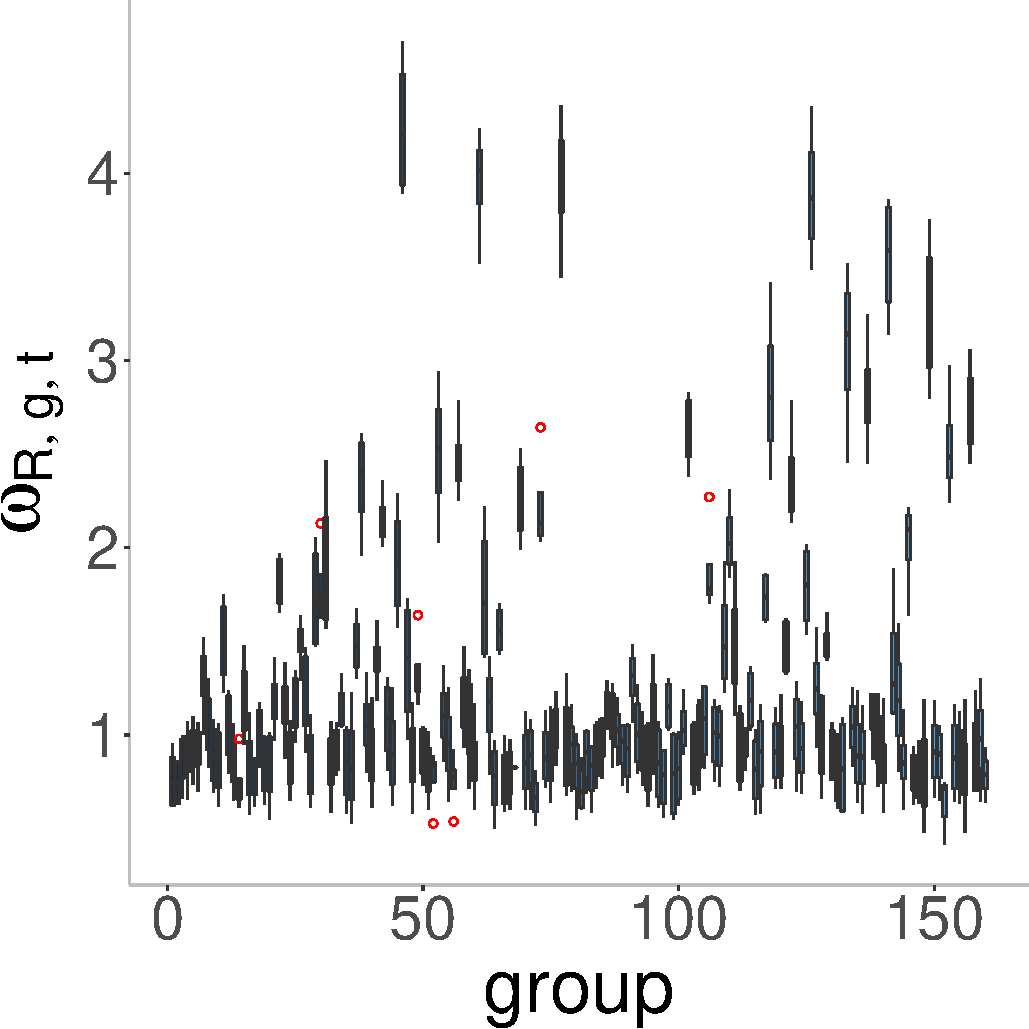
\includegraphics[width = 5in, height =3in]{figs/weightsDiverse}
% Created by tikzDevice version 0.12.3.1 on 2023-11-03 10:48:02
% !TEX encoding = UTF-8 Unicode
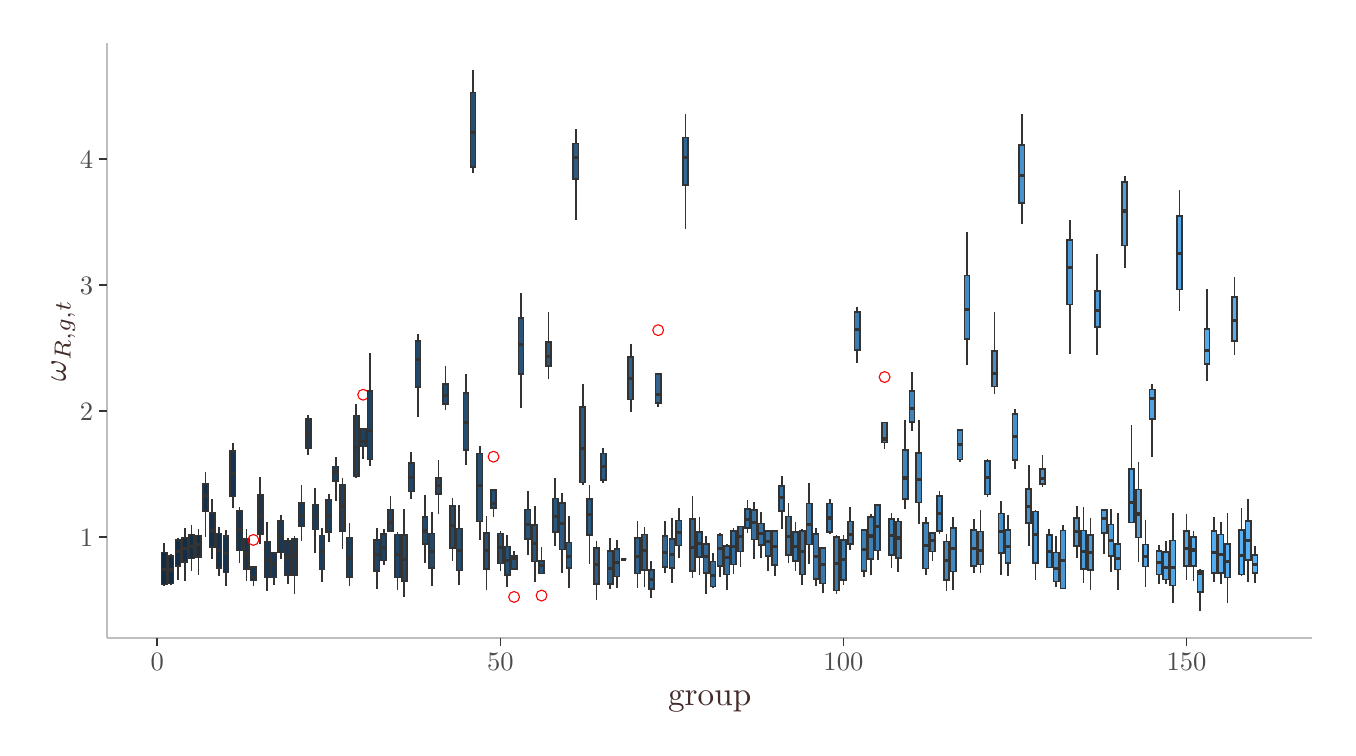
\begin{tikzpicture}[x=1pt,y=1pt]
\definecolor{fillColor}{RGB}{255,255,255}
\path[use as bounding box,fill=fillColor,fill opacity=0.00] (0,0) rectangle (469.75,252.94);
\begin{scope}
\path[clip] (  0.00,  0.00) rectangle (469.75,252.94);
\definecolor{drawColor}{RGB}{255,255,255}
\definecolor{fillColor}{RGB}{255,255,255}

\path[draw=drawColor,line width= 0.6pt,line join=round,line cap=round,fill=fillColor] (  0.00,  0.00) rectangle (469.76,252.94);
\end{scope}
\begin{scope}
\path[clip] ( 28.60, 32.28) rectangle (464.25,247.44);
\definecolor{drawColor}{RGB}{255,255,255}

\path[draw=drawColor,line width= 0.6pt,line join=round] ( 28.60, 68.78) --
	(464.25, 68.78);

\path[draw=drawColor,line width= 0.6pt,line join=round] ( 28.60,114.35) --
	(464.25,114.35);

\path[draw=drawColor,line width= 0.6pt,line join=round] ( 28.60,159.93) --
	(464.25,159.93);

\path[draw=drawColor,line width= 0.6pt,line join=round] ( 28.60,205.51) --
	(464.25,205.51);

\path[draw=drawColor,line width= 0.6pt,line join=round] ( 46.85, 32.28) --
	( 46.85,247.44);

\path[draw=drawColor,line width= 0.6pt,line join=round] (170.81, 32.28) --
	(170.81,247.44);

\path[draw=drawColor,line width= 0.6pt,line join=round] (294.77, 32.28) --
	(294.77,247.44);

\path[draw=drawColor,line width= 0.6pt,line join=round] (418.73, 32.28) --
	(418.73,247.44);
\definecolor{drawColor}{gray}{0.20}

\path[draw=drawColor,line width= 0.6pt,line join=round] ( 49.33, 63.31) -- ( 49.33, 66.76);

\path[draw=drawColor,line width= 0.6pt,line join=round] ( 49.33, 51.72) -- ( 49.33, 51.31);
\definecolor{fillColor}{RGB}{19,43,67}

\path[draw=drawColor,line width= 0.6pt,fill=fillColor] ( 48.40, 63.31) --
	( 48.40, 51.72) --
	( 50.26, 51.72) --
	( 50.26, 63.31) --
	( 48.40, 63.31) --
	cycle;

\path[draw=drawColor,line width= 1.1pt] ( 48.40, 57.01) -- ( 50.26, 57.01);

\path[draw=drawColor,line width= 0.6pt,line join=round] ( 51.81, 62.06) -- ( 51.81, 62.68);

\path[draw=drawColor,line width= 0.6pt,line join=round] ( 51.81, 52.08) -- ( 51.81, 52.07);
\definecolor{fillColor}{RGB}{19,44,68}

\path[draw=drawColor,line width= 0.6pt,fill=fillColor] ( 50.88, 62.06) --
	( 50.88, 52.08) --
	( 52.74, 52.08) --
	( 52.74, 62.06) --
	( 50.88, 62.06) --
	cycle;

\path[draw=drawColor,line width= 1.1pt] ( 50.88, 56.97) -- ( 52.74, 56.97);

\path[draw=drawColor,line width= 0.6pt,line join=round] ( 54.29, 67.76) -- ( 54.29, 68.60);

\path[draw=drawColor,line width= 0.6pt,line join=round] ( 54.29, 58.32) -- ( 54.29, 53.37);
\definecolor{fillColor}{RGB}{20,44,69}

\path[draw=drawColor,line width= 0.6pt,fill=fillColor] ( 53.36, 67.76) --
	( 53.36, 58.32) --
	( 55.22, 58.32) --
	( 55.22, 67.76) --
	( 53.36, 67.76) --
	cycle;

\path[draw=drawColor,line width= 1.1pt] ( 53.36, 63.73) -- ( 55.22, 63.73);

\path[draw=drawColor,line width= 0.6pt,line join=round] ( 56.77, 68.45) -- ( 56.77, 72.10);

\path[draw=drawColor,line width= 0.6pt,line join=round] ( 56.77, 59.86) -- ( 56.77, 53.17);
\definecolor{fillColor}{RGB}{20,45,70}

\path[draw=drawColor,line width= 0.6pt,fill=fillColor] ( 55.84, 68.45) --
	( 55.84, 59.86) --
	( 57.70, 59.86) --
	( 57.70, 68.45) --
	( 55.84, 68.45) --
	cycle;

\path[draw=drawColor,line width= 1.1pt] ( 55.84, 64.66) -- ( 57.70, 64.66);

\path[draw=drawColor,line width= 0.6pt,line join=round] ( 59.25, 69.75) -- ( 59.25, 73.17);

\path[draw=drawColor,line width= 0.6pt,line join=round] ( 59.25, 61.08) -- ( 59.25, 56.76);
\definecolor{fillColor}{RGB}{20,46,71}

\path[draw=drawColor,line width= 0.6pt,fill=fillColor] ( 58.32, 69.75) --
	( 58.32, 61.08) --
	( 60.18, 61.08) --
	( 60.18, 69.75) --
	( 58.32, 69.75) --
	cycle;

\path[draw=drawColor,line width= 1.1pt] ( 58.32, 65.57) -- ( 60.18, 65.57);

\path[draw=drawColor,line width= 0.6pt,line join=round] ( 61.72, 69.42) -- ( 61.72, 71.77);

\path[draw=drawColor,line width= 0.6pt,line join=round] ( 61.72, 61.60) -- ( 61.72, 55.08);
\definecolor{fillColor}{RGB}{21,47,72}

\path[draw=drawColor,line width= 0.6pt,fill=fillColor] ( 60.79, 69.42) --
	( 60.79, 61.60) --
	( 62.65, 61.60) --
	( 62.65, 69.42) --
	( 60.79, 69.42) --
	cycle;

\path[draw=drawColor,line width= 1.1pt] ( 60.79, 66.20) -- ( 62.65, 66.20);

\path[draw=drawColor,line width= 0.6pt,line join=round] ( 64.20, 87.93) -- ( 64.20, 92.50);

\path[draw=drawColor,line width= 0.6pt,line join=round] ( 64.20, 78.33) -- ( 64.20, 68.97);
\definecolor{fillColor}{RGB}{21,47,73}

\path[draw=drawColor,line width= 0.6pt,fill=fillColor] ( 63.27, 87.93) --
	( 63.27, 78.33) --
	( 65.13, 78.33) --
	( 65.13, 87.93) --
	( 63.27, 87.93) --
	cycle;

\path[draw=drawColor,line width= 1.1pt] ( 63.27, 83.93) -- ( 65.13, 83.93);

\path[draw=drawColor,line width= 0.6pt,line join=round] ( 66.68, 77.57) -- ( 66.68, 82.47);

\path[draw=drawColor,line width= 0.6pt,line join=round] ( 66.68, 65.30) -- ( 66.68, 60.79);
\definecolor{fillColor}{RGB}{22,48,74}

\path[draw=drawColor,line width= 0.6pt,fill=fillColor] ( 65.75, 77.57) --
	( 65.75, 65.30) --
	( 67.61, 65.30) --
	( 67.61, 77.57) --
	( 65.75, 77.57) --
	cycle;

\path[draw=drawColor,line width= 1.1pt] ( 65.75, 71.37) -- ( 67.61, 71.37);

\path[draw=drawColor,line width= 0.6pt,line join=round] ( 69.16, 70.17) -- ( 69.16, 72.48);

\path[draw=drawColor,line width= 0.6pt,line join=round] ( 69.16, 57.70) -- ( 69.16, 54.89);
\definecolor{fillColor}{RGB}{22,49,75}

\path[draw=drawColor,line width= 0.6pt,fill=fillColor] ( 68.23, 70.17) --
	( 68.23, 57.70) --
	( 70.09, 57.70) --
	( 70.09, 70.17) --
	( 68.23, 70.17) --
	cycle;

\path[draw=drawColor,line width= 1.1pt] ( 68.23, 64.02) -- ( 70.09, 64.02);

\path[draw=drawColor,line width= 0.6pt,line join=round] ( 71.64, 69.25) -- ( 71.64, 71.46);

\path[draw=drawColor,line width= 0.6pt,line join=round] ( 71.64, 56.09) -- ( 71.64, 51.27);
\definecolor{fillColor}{RGB}{22,50,76}

\path[draw=drawColor,line width= 0.6pt,fill=fillColor] ( 70.71, 69.25) --
	( 70.71, 56.09) --
	( 72.57, 56.09) --
	( 72.57, 69.25) --
	( 70.71, 69.25) --
	cycle;

\path[draw=drawColor,line width= 1.1pt] ( 70.71, 63.10) -- ( 72.57, 63.10);

\path[draw=drawColor,line width= 0.6pt,line join=round] ( 74.12, 99.91) -- ( 74.12,102.91);

\path[draw=drawColor,line width= 0.6pt,line join=round] ( 74.12, 83.55) -- ( 74.12, 79.21);
\definecolor{fillColor}{RGB}{23,50,77}

\path[draw=drawColor,line width= 0.6pt,fill=fillColor] ( 73.19, 99.91) --
	( 73.19, 83.55) --
	( 75.05, 83.55) --
	( 75.05, 99.91) --
	( 73.19, 99.91) --
	cycle;

\path[draw=drawColor,line width= 1.1pt] ( 73.19, 91.96) -- ( 75.05, 91.96);

\path[draw=drawColor,line width= 0.6pt,line join=round] ( 76.60, 78.25) -- ( 76.60, 79.59);

\path[draw=drawColor,line width= 0.6pt,line join=round] ( 76.60, 63.99) -- ( 76.60, 59.42);
\definecolor{fillColor}{RGB}{23,51,78}

\path[draw=drawColor,line width= 0.6pt,fill=fillColor] ( 75.67, 78.25) --
	( 75.67, 63.99) --
	( 77.53, 63.99) --
	( 77.53, 78.25) --
	( 75.67, 78.25) --
	cycle;

\path[draw=drawColor,line width= 1.1pt] ( 75.67, 71.66) -- ( 77.53, 71.66);

\path[draw=drawColor,line width= 0.6pt,line join=round] ( 79.08, 68.41) -- ( 79.08, 71.70);

\path[draw=drawColor,line width= 0.6pt,line join=round] ( 79.08, 57.38) -- ( 79.08, 52.83);
\definecolor{fillColor}{RGB}{24,52,79}

\path[draw=drawColor,line width= 0.6pt,fill=fillColor] ( 78.15, 68.41) --
	( 78.15, 57.38) --
	( 80.01, 57.38) --
	( 80.01, 68.41) --
	( 78.15, 68.41) --
	cycle;

\path[draw=drawColor,line width= 1.1pt] ( 78.15, 63.10) -- ( 80.01, 63.10);
\definecolor{drawColor}{RGB}{255,0,0}

\path[draw=drawColor,line width= 0.4pt,line join=round,line cap=round] ( 81.56, 67.84) circle (  1.96);
\definecolor{drawColor}{gray}{0.20}

\path[draw=drawColor,line width= 0.6pt,line join=round] ( 81.56, 58.14) -- ( 81.56, 58.14);

\path[draw=drawColor,line width= 0.6pt,line join=round] ( 81.56, 53.22) -- ( 81.56, 51.02);
\definecolor{fillColor}{RGB}{24,53,80}

\path[draw=drawColor,line width= 0.6pt,fill=fillColor] ( 80.63, 58.14) --
	( 80.63, 53.22) --
	( 82.49, 53.22) --
	( 82.49, 58.14) --
	( 80.63, 58.14) --
	cycle;

\path[draw=drawColor,line width= 1.1pt] ( 80.63, 54.43) -- ( 82.49, 54.43);

\path[draw=drawColor,line width= 0.6pt,line join=round] ( 84.04, 84.23) -- ( 84.04, 90.49);

\path[draw=drawColor,line width= 0.6pt,line join=round] ( 84.04, 69.95) -- ( 84.04, 66.51);
\definecolor{fillColor}{RGB}{24,53,81}

\path[draw=drawColor,line width= 0.6pt,fill=fillColor] ( 83.11, 84.23) --
	( 83.11, 69.95) --
	( 84.97, 69.95) --
	( 84.97, 84.23) --
	( 83.11, 84.23) --
	cycle;

\path[draw=drawColor,line width= 1.1pt] ( 83.11, 76.62) -- ( 84.97, 76.62);

\path[draw=drawColor,line width= 0.6pt,line join=round] ( 86.52, 67.23) -- ( 86.52, 74.14);

\path[draw=drawColor,line width= 0.6pt,line join=round] ( 86.52, 54.28) -- ( 86.52, 49.52);
\definecolor{fillColor}{RGB}{25,54,82}

\path[draw=drawColor,line width= 0.6pt,fill=fillColor] ( 85.59, 67.23) --
	( 85.59, 54.28) --
	( 87.45, 54.28) --
	( 87.45, 67.23) --
	( 85.59, 67.23) --
	cycle;

\path[draw=drawColor,line width= 1.1pt] ( 85.59, 60.40) -- ( 87.45, 60.40);

\path[draw=drawColor,line width= 0.6pt,line join=round] ( 89.00, 63.12) -- ( 89.00, 63.34);

\path[draw=drawColor,line width= 0.6pt,line join=round] ( 89.00, 54.21) -- ( 89.00, 51.47);
\definecolor{fillColor}{RGB}{25,55,83}

\path[draw=drawColor,line width= 0.6pt,fill=fillColor] ( 88.07, 63.12) --
	( 88.07, 54.21) --
	( 89.93, 54.21) --
	( 89.93, 63.12) --
	( 88.07, 63.12) --
	cycle;

\path[draw=drawColor,line width= 1.1pt] ( 88.07, 59.08) -- ( 89.93, 59.08);

\path[draw=drawColor,line width= 0.6pt,line join=round] ( 91.48, 74.67) -- ( 91.48, 76.76);

\path[draw=drawColor,line width= 0.6pt,line join=round] ( 91.48, 63.45) -- ( 91.48, 60.90);
\definecolor{fillColor}{RGB}{25,56,84}

\path[draw=drawColor,line width= 0.6pt,fill=fillColor] ( 90.55, 74.67) --
	( 90.55, 63.45) --
	( 92.40, 63.45) --
	( 92.40, 74.67) --
	( 90.55, 74.67) --
	cycle;

\path[draw=drawColor,line width= 1.1pt] ( 90.55, 69.14) -- ( 92.40, 69.14);

\path[draw=drawColor,line width= 0.6pt,line join=round] ( 93.95, 67.34) -- ( 93.95, 68.56);

\path[draw=drawColor,line width= 0.6pt,line join=round] ( 93.95, 55.24) -- ( 93.95, 51.81);
\definecolor{fillColor}{RGB}{26,56,85}

\path[draw=drawColor,line width= 0.6pt,fill=fillColor] ( 93.02, 67.34) --
	( 93.02, 55.24) --
	( 94.88, 55.24) --
	( 94.88, 67.34) --
	( 93.02, 67.34) --
	cycle;

\path[draw=drawColor,line width= 1.1pt] ( 93.02, 61.66) -- ( 94.88, 61.66);

\path[draw=drawColor,line width= 0.6pt,line join=round] ( 96.43, 68.29) -- ( 96.43, 69.28);

\path[draw=drawColor,line width= 0.6pt,line join=round] ( 96.43, 55.12) -- ( 96.43, 48.12);
\definecolor{fillColor}{RGB}{26,57,86}

\path[draw=drawColor,line width= 0.6pt,fill=fillColor] ( 95.50, 68.29) --
	( 95.50, 55.12) --
	( 97.36, 55.12) --
	( 97.36, 68.29) --
	( 95.50, 68.29) --
	cycle;

\path[draw=drawColor,line width= 1.1pt] ( 95.50, 62.70) -- ( 97.36, 62.70);

\path[draw=drawColor,line width= 0.6pt,line join=round] ( 98.91, 81.07) -- ( 98.91, 87.72);

\path[draw=drawColor,line width= 0.6pt,line join=round] ( 98.91, 72.74) -- ( 98.91, 67.49);
\definecolor{fillColor}{RGB}{27,58,87}

\path[draw=drawColor,line width= 0.6pt,fill=fillColor] ( 97.98, 81.07) --
	( 97.98, 72.74) --
	( 99.84, 72.74) --
	( 99.84, 81.07) --
	( 97.98, 81.07) --
	cycle;

\path[draw=drawColor,line width= 1.1pt] ( 97.98, 76.67) -- ( 99.84, 76.67);

\path[draw=drawColor,line width= 0.6pt,line join=round] (101.39,111.52) -- (101.39,112.96);

\path[draw=drawColor,line width= 0.6pt,line join=round] (101.39,100.85) -- (101.39, 98.65);
\definecolor{fillColor}{RGB}{27,59,88}

\path[draw=drawColor,line width= 0.6pt,fill=fillColor] (100.46,111.52) --
	(100.46,100.85) --
	(102.32,100.85) --
	(102.32,111.52) --
	(100.46,111.52) --
	cycle;

\path[draw=drawColor,line width= 1.1pt] (100.46,106.31) -- (102.32,106.31);

\path[draw=drawColor,line width= 0.6pt,line join=round] (103.87, 80.50) -- (103.87, 86.54);

\path[draw=drawColor,line width= 0.6pt,line join=round] (103.87, 71.56) -- (103.87, 63.04);
\definecolor{fillColor}{RGB}{27,60,89}

\path[draw=drawColor,line width= 0.6pt,fill=fillColor] (102.94, 80.50) --
	(102.94, 71.56) --
	(104.80, 71.56) --
	(104.80, 80.50) --
	(102.94, 80.50) --
	cycle;

\path[draw=drawColor,line width= 1.1pt] (102.94, 76.45) -- (104.80, 76.45);

\path[draw=drawColor,line width= 0.6pt,line join=round] (106.35, 69.47) -- (106.35, 72.21);

\path[draw=drawColor,line width= 0.6pt,line join=round] (106.35, 57.12) -- (106.35, 52.79);
\definecolor{fillColor}{RGB}{28,60,90}

\path[draw=drawColor,line width= 0.6pt,fill=fillColor] (105.42, 69.47) --
	(105.42, 57.12) --
	(107.28, 57.12) --
	(107.28, 69.47) --
	(105.42, 69.47) --
	cycle;

\path[draw=drawColor,line width= 1.1pt] (105.42, 63.56) -- (107.28, 63.56);

\path[draw=drawColor,line width= 0.6pt,line join=round] (108.83, 82.40) -- (108.83, 84.37);

\path[draw=drawColor,line width= 0.6pt,line join=round] (108.83, 70.68) -- (108.83, 66.94);
\definecolor{fillColor}{RGB}{28,61,91}

\path[draw=drawColor,line width= 0.6pt,fill=fillColor] (107.90, 82.40) --
	(107.90, 70.68) --
	(109.76, 70.68) --
	(109.76, 82.40) --
	(107.90, 82.40) --
	cycle;

\path[draw=drawColor,line width= 1.1pt] (107.90, 76.83) -- (109.76, 76.83);

\path[draw=drawColor,line width= 0.6pt,line join=round] (111.31, 94.39) -- (111.31, 97.97);

\path[draw=drawColor,line width= 0.6pt,line join=round] (111.31, 89.17) -- (111.31, 81.94);
\definecolor{fillColor}{RGB}{29,62,92}

\path[draw=drawColor,line width= 0.6pt,fill=fillColor] (110.38, 94.39) --
	(110.38, 89.17) --
	(112.24, 89.17) --
	(112.24, 94.39) --
	(110.38, 94.39) --
	cycle;

\path[draw=drawColor,line width= 1.1pt] (110.38, 92.38) -- (112.24, 92.38);

\path[draw=drawColor,line width= 0.6pt,line join=round] (113.79, 87.73) -- (113.79, 90.14);

\path[draw=drawColor,line width= 0.6pt,line join=round] (113.79, 71.04) -- (113.79, 64.53);
\definecolor{fillColor}{RGB}{29,63,93}

\path[draw=drawColor,line width= 0.6pt,fill=fillColor] (112.86, 87.73) --
	(112.86, 71.04) --
	(114.72, 71.04) --
	(114.72, 87.73) --
	(112.86, 87.73) --
	cycle;

\path[draw=drawColor,line width= 1.1pt] (112.86, 80.07) -- (114.72, 80.07);

\path[draw=drawColor,line width= 0.6pt,line join=round] (116.27, 68.74) -- (116.27, 73.86);

\path[draw=drawColor,line width= 0.6pt,line join=round] (116.27, 54.46) -- (116.27, 51.09);
\definecolor{fillColor}{RGB}{29,63,94}

\path[draw=drawColor,line width= 0.6pt,fill=fillColor] (115.34, 68.74) --
	(115.34, 54.46) --
	(117.20, 54.46) --
	(117.20, 68.74) --
	(115.34, 68.74) --
	cycle;

\path[draw=drawColor,line width= 1.1pt] (115.34, 61.31) -- (117.20, 61.31);

\path[draw=drawColor,line width= 0.6pt,line join=round] (118.75,112.81) -- (118.75,116.93);

\path[draw=drawColor,line width= 0.6pt,line join=round] (118.75, 91.03) -- (118.75, 90.27);
\definecolor{fillColor}{RGB}{30,64,96}

\path[draw=drawColor,line width= 0.6pt,fill=fillColor] (117.82,112.81) --
	(117.82, 91.03) --
	(119.68, 91.03) --
	(119.68,112.81) --
	(117.82,112.81) --
	cycle;

\path[draw=drawColor,line width= 1.1pt] (117.82,101.36) -- (119.68,101.36);
\definecolor{drawColor}{RGB}{255,0,0}

\path[draw=drawColor,line width= 0.4pt,line join=round,line cap=round] (121.23,120.30) circle (  1.96);
\definecolor{drawColor}{gray}{0.20}

\path[draw=drawColor,line width= 0.6pt,line join=round] (121.23,107.84) -- (121.23,107.84);

\path[draw=drawColor,line width= 0.6pt,line join=round] (121.23,101.64) -- (121.23, 97.15);
\definecolor{fillColor}{RGB}{30,65,97}

\path[draw=drawColor,line width= 0.6pt,fill=fillColor] (120.30,107.84) --
	(120.30,101.64) --
	(122.16,101.64) --
	(122.16,107.84) --
	(120.30,107.84) --
	cycle;

\path[draw=drawColor,line width= 1.1pt] (120.30,103.41) -- (122.16,103.41);

\path[draw=drawColor,line width= 0.6pt,line join=round] (123.70,121.72) -- (123.70,135.52);

\path[draw=drawColor,line width= 0.6pt,line join=round] (123.70, 96.90) -- (123.70, 94.72);
\definecolor{fillColor}{RGB}{31,66,98}

\path[draw=drawColor,line width= 0.6pt,fill=fillColor] (122.78,121.72) --
	(122.78, 96.90) --
	(124.63, 96.90) --
	(124.63,121.72) --
	(122.78,121.72) --
	cycle;

\path[draw=drawColor,line width= 1.1pt] (122.78,107.38) -- (124.63,107.38);

\path[draw=drawColor,line width= 0.6pt,line join=round] (126.18, 67.84) -- (126.18, 72.13);

\path[draw=drawColor,line width= 0.6pt,line join=round] (126.18, 56.69) -- (126.18, 49.96);
\definecolor{fillColor}{RGB}{31,67,99}

\path[draw=drawColor,line width= 0.6pt,fill=fillColor] (125.25, 67.84) --
	(125.25, 56.69) --
	(127.11, 56.69) --
	(127.11, 67.84) --
	(125.25, 67.84) --
	cycle;

\path[draw=drawColor,line width= 1.1pt] (125.25, 62.67) -- (127.11, 62.67);

\path[draw=drawColor,line width= 0.6pt,line join=round] (128.66, 69.89) -- (128.66, 71.85);

\path[draw=drawColor,line width= 0.6pt,line join=round] (128.66, 60.37) -- (128.66, 58.88);
\definecolor{fillColor}{RGB}{31,67,100}

\path[draw=drawColor,line width= 0.6pt,fill=fillColor] (127.73, 69.89) --
	(127.73, 60.37) --
	(129.59, 60.37) --
	(129.59, 69.89) --
	(127.73, 69.89) --
	cycle;

\path[draw=drawColor,line width= 1.1pt] (127.73, 65.05) -- (129.59, 65.05);

\path[draw=drawColor,line width= 0.6pt,line join=round] (131.14, 78.89) -- (131.14, 83.85);

\path[draw=drawColor,line width= 0.6pt,line join=round] (131.14, 71.17) -- (131.14, 70.71);
\definecolor{fillColor}{RGB}{32,68,101}

\path[draw=drawColor,line width= 0.6pt,fill=fillColor] (130.21, 78.89) --
	(130.21, 71.17) --
	(132.07, 71.17) --
	(132.07, 78.89) --
	(130.21, 78.89) --
	cycle;

\path[draw=drawColor,line width= 1.1pt] (130.21, 74.28) -- (132.07, 74.28);

\path[draw=drawColor,line width= 0.6pt,line join=round] (133.62, 69.82) -- (133.62, 70.82);

\path[draw=drawColor,line width= 0.6pt,line join=round] (133.62, 54.31) -- (133.62, 49.73);
\definecolor{fillColor}{RGB}{32,69,102}

\path[draw=drawColor,line width= 0.6pt,fill=fillColor] (132.69, 69.82) --
	(132.69, 54.31) --
	(134.55, 54.31) --
	(134.55, 69.82) --
	(132.69, 69.82) --
	cycle;

\path[draw=drawColor,line width= 1.1pt] (132.69, 62.66) -- (134.55, 62.66);

\path[draw=drawColor,line width= 0.6pt,line join=round] (136.10, 69.67) -- (136.10, 79.06);

\path[draw=drawColor,line width= 0.6pt,line join=round] (136.10, 53.01) -- (136.10, 47.33);
\definecolor{fillColor}{RGB}{33,70,103}

\path[draw=drawColor,line width= 0.6pt,fill=fillColor] (135.17, 69.67) --
	(135.17, 53.01) --
	(137.03, 53.01) --
	(137.03, 69.67) --
	(135.17, 69.67) --
	cycle;

\path[draw=drawColor,line width= 1.1pt] (135.17, 60.72) -- (137.03, 60.72);

\path[draw=drawColor,line width= 0.6pt,line join=round] (138.58, 95.72) -- (138.58, 99.48);

\path[draw=drawColor,line width= 0.6pt,line join=round] (138.58, 85.32) -- (138.58, 82.53);
\definecolor{fillColor}{RGB}{33,70,104}

\path[draw=drawColor,line width= 0.6pt,fill=fillColor] (137.65, 95.72) --
	(137.65, 85.32) --
	(139.51, 85.32) --
	(139.51, 95.72) --
	(137.65, 95.72) --
	cycle;

\path[draw=drawColor,line width= 1.1pt] (137.65, 90.35) -- (139.51, 90.35);

\path[draw=drawColor,line width= 0.6pt,line join=round] (141.06,139.82) -- (141.06,142.20);

\path[draw=drawColor,line width= 0.6pt,line join=round] (141.06,123.21) -- (141.06,112.39);
\definecolor{fillColor}{RGB}{33,71,105}

\path[draw=drawColor,line width= 0.6pt,fill=fillColor] (140.13,139.82) --
	(140.13,123.21) --
	(141.99,123.21) --
	(141.99,139.82) --
	(140.13,139.82) --
	cycle;

\path[draw=drawColor,line width= 1.1pt] (140.13,132.92) -- (141.99,132.92);

\path[draw=drawColor,line width= 0.6pt,line join=round] (143.54, 76.21) -- (143.54, 83.91);

\path[draw=drawColor,line width= 0.6pt,line join=round] (143.54, 66.27) -- (143.54, 59.65);
\definecolor{fillColor}{RGB}{34,72,106}

\path[draw=drawColor,line width= 0.6pt,fill=fillColor] (142.61, 76.21) --
	(142.61, 66.27) --
	(144.47, 66.27) --
	(144.47, 76.21) --
	(142.61, 76.21) --
	cycle;

\path[draw=drawColor,line width= 1.1pt] (142.61, 71.06) -- (144.47, 71.06);

\path[draw=drawColor,line width= 0.6pt,line join=round] (146.02, 70.12) -- (146.02, 77.95);

\path[draw=drawColor,line width= 0.6pt,line join=round] (146.02, 57.68) -- (146.02, 51.08);
\definecolor{fillColor}{RGB}{34,73,107}

\path[draw=drawColor,line width= 0.6pt,fill=fillColor] (145.09, 70.12) --
	(145.09, 57.68) --
	(146.95, 57.68) --
	(146.95, 70.12) --
	(145.09, 70.12) --
	cycle;

\path[draw=drawColor,line width= 1.1pt] (145.09, 63.69) -- (146.95, 63.69);

\path[draw=drawColor,line width= 0.6pt,line join=round] (148.50, 90.15) -- (148.50, 96.71);

\path[draw=drawColor,line width= 0.6pt,line join=round] (148.50, 84.37) -- (148.50, 77.22);
\definecolor{fillColor}{RGB}{34,74,108}

\path[draw=drawColor,line width= 0.6pt,fill=fillColor] (147.57, 90.15) --
	(147.57, 84.37) --
	(149.43, 84.37) --
	(149.43, 90.15) --
	(147.57, 90.15) --
	cycle;

\path[draw=drawColor,line width= 1.1pt] (147.57, 87.36) -- (149.43, 87.36);

\path[draw=drawColor,line width= 0.6pt,line join=round] (150.98,124.22) -- (150.98,130.75);

\path[draw=drawColor,line width= 0.6pt,line join=round] (150.98,117.03) -- (150.98,114.73);
\definecolor{fillColor}{RGB}{35,74,109}

\path[draw=drawColor,line width= 0.6pt,fill=fillColor] (150.05,124.22) --
	(150.05,117.03) --
	(151.91,117.03) --
	(151.91,124.22) --
	(150.05,124.22) --
	cycle;

\path[draw=drawColor,line width= 1.1pt] (150.05,119.92) -- (151.91,119.92);

\path[draw=drawColor,line width= 0.6pt,line join=round] (153.46, 80.21) -- (153.46, 82.87);

\path[draw=drawColor,line width= 0.6pt,line join=round] (153.46, 65.00) -- (153.46, 60.20);
\definecolor{fillColor}{RGB}{35,75,110}

\path[draw=drawColor,line width= 0.6pt,fill=fillColor] (152.53, 80.21) --
	(152.53, 65.00) --
	(154.39, 65.00) --
	(154.39, 80.21) --
	(152.53, 80.21) --
	cycle;

\path[draw=drawColor,line width= 1.1pt] (152.53, 72.97) -- (154.39, 72.97);

\path[draw=drawColor,line width= 0.6pt,line join=round] (155.93, 72.00) -- (155.93, 80.31);

\path[draw=drawColor,line width= 0.6pt,line join=round] (155.93, 56.82) -- (155.93, 51.60);
\definecolor{fillColor}{RGB}{36,76,111}

\path[draw=drawColor,line width= 0.6pt,fill=fillColor] (155.00, 72.00) --
	(155.00, 56.82) --
	(156.86, 56.82) --
	(156.86, 72.00) --
	(155.00, 72.00) --
	cycle;

\path[draw=drawColor,line width= 1.1pt] (155.00, 63.90) -- (156.86, 63.90);

\path[draw=drawColor,line width= 0.6pt,line join=round] (158.41,120.81) -- (158.41,127.67);

\path[draw=drawColor,line width= 0.6pt,line join=round] (158.41,100.36) -- (158.41, 94.86);
\definecolor{fillColor}{RGB}{36,77,113}

\path[draw=drawColor,line width= 0.6pt,fill=fillColor] (157.48,120.81) --
	(157.48,100.36) --
	(159.34,100.36) --
	(159.34,120.81) --
	(157.48,120.81) --
	cycle;

\path[draw=drawColor,line width= 1.1pt] (157.48,110.36) -- (159.34,110.36);

\path[draw=drawColor,line width= 0.6pt,line join=round] (160.89,229.48) -- (160.89,237.66);

\path[draw=drawColor,line width= 0.6pt,line join=round] (160.89,202.65) -- (160.89,200.60);
\definecolor{fillColor}{RGB}{37,78,114}

\path[draw=drawColor,line width= 0.6pt,fill=fillColor] (159.96,229.48) --
	(159.96,202.65) --
	(161.82,202.65) --
	(161.82,229.48) --
	(159.96,229.48) --
	cycle;

\path[draw=drawColor,line width= 1.1pt] (159.96,215.04) -- (161.82,215.04);

\path[draw=drawColor,line width= 0.6pt,line join=round] (163.37, 99.03) -- (163.37,101.91);

\path[draw=drawColor,line width= 0.6pt,line join=round] (163.37, 74.54) -- (163.37, 67.66);
\definecolor{fillColor}{RGB}{37,78,115}

\path[draw=drawColor,line width= 0.6pt,fill=fillColor] (162.44, 99.03) --
	(162.44, 74.54) --
	(164.30, 74.54) --
	(164.30, 99.03) --
	(162.44, 99.03) --
	cycle;

\path[draw=drawColor,line width= 1.1pt] (162.44, 87.46) -- (164.30, 87.46);

\path[draw=drawColor,line width= 0.6pt,line join=round] (165.85, 70.29) -- (165.85, 76.62);

\path[draw=drawColor,line width= 0.6pt,line join=round] (165.85, 57.39) -- (165.85, 49.69);
\definecolor{fillColor}{RGB}{37,79,116}

\path[draw=drawColor,line width= 0.6pt,fill=fillColor] (164.92, 70.29) --
	(164.92, 57.39) --
	(166.78, 57.39) --
	(166.78, 70.29) --
	(164.92, 70.29) --
	cycle;

\path[draw=drawColor,line width= 1.1pt] (164.92, 64.07) -- (166.78, 64.07);
\definecolor{drawColor}{RGB}{255,0,0}

\path[draw=drawColor,line width= 0.4pt,line join=round,line cap=round] (168.33, 97.91) circle (  1.96);
\definecolor{drawColor}{gray}{0.20}

\path[draw=drawColor,line width= 0.6pt,line join=round] (168.33, 85.82) -- (168.33, 85.82);

\path[draw=drawColor,line width= 0.6pt,line join=round] (168.33, 79.46) -- (168.33, 76.20);
\definecolor{fillColor}{RGB}{38,80,117}

\path[draw=drawColor,line width= 0.6pt,fill=fillColor] (167.40, 85.82) --
	(167.40, 79.46) --
	(169.26, 79.46) --
	(169.26, 85.82) --
	(167.40, 85.82) --
	cycle;

\path[draw=drawColor,line width= 1.1pt] (167.40, 81.17) -- (169.26, 81.17);

\path[draw=drawColor,line width= 0.6pt,line join=round] (170.81, 70.20) -- (170.81, 70.90);

\path[draw=drawColor,line width= 0.6pt,line join=round] (170.81, 59.35) -- (170.81, 56.60);
\definecolor{fillColor}{RGB}{38,81,118}

\path[draw=drawColor,line width= 0.6pt,fill=fillColor] (169.88, 70.20) --
	(169.88, 59.35) --
	(171.74, 59.35) --
	(171.74, 70.20) --
	(169.88, 70.20) --
	cycle;

\path[draw=drawColor,line width= 1.1pt] (169.88, 65.11) -- (171.74, 65.11);

\path[draw=drawColor,line width= 0.6pt,line join=round] (173.29, 65.52) -- (173.29, 69.58);

\path[draw=drawColor,line width= 0.6pt,line join=round] (173.29, 55.10) -- (173.29, 50.65);
\definecolor{fillColor}{RGB}{39,82,119}

\path[draw=drawColor,line width= 0.6pt,fill=fillColor] (172.36, 65.52) --
	(172.36, 55.10) --
	(174.22, 55.10) --
	(174.22, 65.52) --
	(172.36, 65.52) --
	cycle;

\path[draw=drawColor,line width= 1.1pt] (172.36, 60.37) -- (174.22, 60.37);
\definecolor{drawColor}{RGB}{255,0,0}

\path[draw=drawColor,line width= 0.4pt,line join=round,line cap=round] (175.77, 47.24) circle (  1.96);
\definecolor{drawColor}{gray}{0.20}

\path[draw=drawColor,line width= 0.6pt,line join=round] (175.77, 62.10) -- (175.77, 63.88);

\path[draw=drawColor,line width= 0.6pt,line join=round] (175.77, 57.33) -- (175.77, 57.33);
\definecolor{fillColor}{RGB}{39,82,120}

\path[draw=drawColor,line width= 0.6pt,fill=fillColor] (174.84, 62.10) --
	(174.84, 57.33) --
	(176.70, 57.33) --
	(176.70, 62.10) --
	(174.84, 62.10) --
	cycle;

\path[draw=drawColor,line width= 1.1pt] (174.84, 61.10) -- (176.70, 61.10);

\path[draw=drawColor,line width= 0.6pt,line join=round] (178.25,148.01) -- (178.25,157.13);

\path[draw=drawColor,line width= 0.6pt,line join=round] (178.25,127.72) -- (178.25,115.64);
\definecolor{fillColor}{RGB}{39,83,121}

\path[draw=drawColor,line width= 0.6pt,fill=fillColor] (177.32,148.01) --
	(177.32,127.72) --
	(179.18,127.72) --
	(179.18,148.01) --
	(177.32,148.01) --
	cycle;

\path[draw=drawColor,line width= 1.1pt] (177.32,138.36) -- (179.18,138.36);

\path[draw=drawColor,line width= 0.6pt,line join=round] (180.73, 78.85) -- (180.73, 85.69);

\path[draw=drawColor,line width= 0.6pt,line join=round] (180.73, 68.28) -- (180.73, 62.44);
\definecolor{fillColor}{RGB}{40,84,122}

\path[draw=drawColor,line width= 0.6pt,fill=fillColor] (179.80, 78.85) --
	(179.80, 68.28) --
	(181.66, 68.28) --
	(181.66, 78.85) --
	(179.80, 78.85) --
	cycle;

\path[draw=drawColor,line width= 1.1pt] (179.80, 73.40) -- (181.66, 73.40);

\path[draw=drawColor,line width= 0.6pt,line join=round] (183.21, 73.13) -- (183.21, 80.25);

\path[draw=drawColor,line width= 0.6pt,line join=round] (183.21, 60.08) -- (183.21, 52.71);
\definecolor{fillColor}{RGB}{40,85,123}

\path[draw=drawColor,line width= 0.6pt,fill=fillColor] (182.28, 73.13) --
	(182.28, 60.08) --
	(184.14, 60.08) --
	(184.14, 73.13) --
	(182.28, 73.13) --
	cycle;

\path[draw=drawColor,line width= 1.1pt] (182.28, 66.65) -- (184.14, 66.65);
\definecolor{drawColor}{RGB}{255,0,0}

\path[draw=drawColor,line width= 0.4pt,line join=round,line cap=round] (185.69, 47.73) circle (  1.96);
\definecolor{drawColor}{gray}{0.20}

\path[draw=drawColor,line width= 0.6pt,line join=round] (185.69, 60.25) -- (185.69, 65.18);

\path[draw=drawColor,line width= 0.6pt,line join=round] (185.69, 55.75) -- (185.69, 55.75);
\definecolor{fillColor}{RGB}{41,86,125}

\path[draw=drawColor,line width= 0.6pt,fill=fillColor] (184.76, 60.25) --
	(184.76, 55.75) --
	(186.61, 55.75) --
	(186.61, 60.25) --
	(184.76, 60.25) --
	cycle;

\path[draw=drawColor,line width= 1.1pt] (184.76, 58.51) -- (186.61, 58.51);

\path[draw=drawColor,line width= 0.6pt,line join=round] (188.16,139.30) -- (188.16,150.08);

\path[draw=drawColor,line width= 0.6pt,line join=round] (188.16,130.66) -- (188.16,125.86);
\definecolor{fillColor}{RGB}{41,87,126}

\path[draw=drawColor,line width= 0.6pt,fill=fillColor] (187.23,139.30) --
	(187.23,130.66) --
	(189.09,130.66) --
	(189.09,139.30) --
	(187.23,139.30) --
	cycle;

\path[draw=drawColor,line width= 1.1pt] (187.23,133.99) -- (189.09,133.99);

\path[draw=drawColor,line width= 0.6pt,line join=round] (190.64, 82.79) -- (190.64, 90.26);

\path[draw=drawColor,line width= 0.6pt,line join=round] (190.64, 70.61) -- (190.64, 65.78);
\definecolor{fillColor}{RGB}{41,87,127}

\path[draw=drawColor,line width= 0.6pt,fill=fillColor] (189.71, 82.79) --
	(189.71, 70.61) --
	(191.57, 70.61) --
	(191.57, 82.79) --
	(189.71, 82.79) --
	cycle;

\path[draw=drawColor,line width= 1.1pt] (189.71, 76.26) -- (191.57, 76.26);

\path[draw=drawColor,line width= 0.6pt,line join=round] (193.12, 81.14) -- (193.12, 84.66);

\path[draw=drawColor,line width= 0.6pt,line join=round] (193.12, 64.35) -- (193.12, 55.73);
\definecolor{fillColor}{RGB}{42,88,128}

\path[draw=drawColor,line width= 0.6pt,fill=fillColor] (192.19, 81.14) --
	(192.19, 64.35) --
	(194.05, 64.35) --
	(194.05, 81.14) --
	(192.19, 81.14) --
	cycle;

\path[draw=drawColor,line width= 1.1pt] (192.19, 73.60) -- (194.05, 73.60);

\path[draw=drawColor,line width= 0.6pt,line join=round] (195.60, 66.96) -- (195.60, 76.34);

\path[draw=drawColor,line width= 0.6pt,line join=round] (195.60, 57.72) -- (195.60, 50.55);
\definecolor{fillColor}{RGB}{42,89,129}

\path[draw=drawColor,line width= 0.6pt,fill=fillColor] (194.67, 66.96) --
	(194.67, 57.72) --
	(196.53, 57.72) --
	(196.53, 66.96) --
	(194.67, 66.96) --
	cycle;

\path[draw=drawColor,line width= 1.1pt] (194.67, 61.97) -- (196.53, 61.97);

\path[draw=drawColor,line width= 0.6pt,line join=round] (198.08,211.07) -- (198.08,216.40);

\path[draw=drawColor,line width= 0.6pt,line join=round] (198.08,198.16) -- (198.08,183.57);
\definecolor{fillColor}{RGB}{43,90,130}

\path[draw=drawColor,line width= 0.6pt,fill=fillColor] (197.15,211.07) --
	(197.15,198.16) --
	(199.01,198.16) --
	(199.01,211.07) --
	(197.15,211.07) --
	cycle;

\path[draw=drawColor,line width= 1.1pt] (197.15,206.16) -- (199.01,206.16);

\path[draw=drawColor,line width= 0.6pt,line join=round] (200.56,115.84) -- (200.56,124.32);

\path[draw=drawColor,line width= 0.6pt,line join=round] (200.56, 88.53) -- (200.56, 87.60);
\definecolor{fillColor}{RGB}{43,91,131}

\path[draw=drawColor,line width= 0.6pt,fill=fillColor] (199.63,115.84) --
	(199.63, 88.53) --
	(201.49, 88.53) --
	(201.49,115.84) --
	(199.63,115.84) --
	cycle;

\path[draw=drawColor,line width= 1.1pt] (199.63,100.93) -- (201.49,100.93);

\path[draw=drawColor,line width= 0.6pt,line join=round] (203.04, 82.60) -- (203.04, 87.83);

\path[draw=drawColor,line width= 0.6pt,line join=round] (203.04, 69.57) -- (203.04, 59.18);
\definecolor{fillColor}{RGB}{43,91,132}

\path[draw=drawColor,line width= 0.6pt,fill=fillColor] (202.11, 82.60) --
	(202.11, 69.57) --
	(203.97, 69.57) --
	(203.97, 82.60) --
	(202.11, 82.60) --
	cycle;

\path[draw=drawColor,line width= 1.1pt] (202.11, 76.94) -- (203.97, 76.94);

\path[draw=drawColor,line width= 0.6pt,line join=round] (205.52, 64.83) -- (205.52, 67.40);

\path[draw=drawColor,line width= 0.6pt,line join=round] (205.52, 51.87) -- (205.52, 46.12);
\definecolor{fillColor}{RGB}{44,92,133}

\path[draw=drawColor,line width= 0.6pt,fill=fillColor] (204.59, 64.83) --
	(204.59, 51.87) --
	(206.45, 51.87) --
	(206.45, 64.83) --
	(204.59, 64.83) --
	cycle;

\path[draw=drawColor,line width= 1.1pt] (204.59, 58.88) -- (206.45, 58.88);

\path[draw=drawColor,line width= 0.6pt,line join=round] (208.00, 99.03) -- (208.00,100.89);

\path[draw=drawColor,line width= 0.6pt,line join=round] (208.00, 89.59) -- (208.00, 88.40);
\definecolor{fillColor}{RGB}{44,93,134}

\path[draw=drawColor,line width= 0.6pt,fill=fillColor] (207.07, 99.03) --
	(207.07, 89.59) --
	(208.93, 89.59) --
	(208.93, 99.03) --
	(207.07, 99.03) --
	cycle;

\path[draw=drawColor,line width= 1.1pt] (207.07, 94.20) -- (208.93, 94.20);

\path[draw=drawColor,line width= 0.6pt,line join=round] (210.48, 63.81) -- (210.48, 68.55);

\path[draw=drawColor,line width= 0.6pt,line join=round] (210.48, 52.02) -- (210.48, 50.18);
\definecolor{fillColor}{RGB}{45,94,136}

\path[draw=drawColor,line width= 0.6pt,fill=fillColor] (209.55, 63.81) --
	(209.55, 52.02) --
	(211.41, 52.02) --
	(211.41, 63.81) --
	(209.55, 63.81) --
	cycle;

\path[draw=drawColor,line width= 1.1pt] (209.55, 57.43) -- (211.41, 57.43);

\path[draw=drawColor,line width= 0.6pt,line join=round] (212.96, 64.58) -- (212.96, 67.70);

\path[draw=drawColor,line width= 0.6pt,line join=round] (212.96, 54.56) -- (212.96, 50.57);
\definecolor{fillColor}{RGB}{45,95,137}

\path[draw=drawColor,line width= 0.6pt,fill=fillColor] (212.03, 64.58) --
	(212.03, 54.56) --
	(213.89, 54.56) --
	(213.89, 64.58) --
	(212.03, 64.58) --
	cycle;

\path[draw=drawColor,line width= 1.1pt] (212.03, 59.71) -- (213.89, 59.71);

\path[draw=drawColor,line width= 0.6pt,line join=round] (215.44, 60.87) -- (215.44, 60.87);

\path[draw=drawColor,line width= 0.6pt,line join=round] (215.44, 60.87) -- (215.44, 60.87);
\definecolor{fillColor}{RGB}{46,96,138}

\path[draw=drawColor,line width= 0.6pt,fill=fillColor] (214.51, 60.87) --
	(214.51, 60.87) --
	(216.37, 60.87) --
	(216.37, 60.87) --
	(214.51, 60.87) --
	cycle;

\path[draw=drawColor,line width= 1.1pt] (214.51, 60.87) -- (216.37, 60.87);

\path[draw=drawColor,line width= 0.6pt,line join=round] (217.91,133.93) -- (217.91,138.51);

\path[draw=drawColor,line width= 0.6pt,line join=round] (217.91,118.58) -- (217.91,113.99);
\definecolor{fillColor}{RGB}{46,96,139}

\path[draw=drawColor,line width= 0.6pt,fill=fillColor] (216.99,133.93) --
	(216.99,118.58) --
	(218.84,118.58) --
	(218.84,133.93) --
	(216.99,133.93) --
	cycle;

\path[draw=drawColor,line width= 1.1pt] (216.99,126.26) -- (218.84,126.26);

\path[draw=drawColor,line width= 0.6pt,line join=round] (220.39, 68.58) -- (220.39, 74.60);

\path[draw=drawColor,line width= 0.6pt,line join=round] (220.39, 55.68) -- (220.39, 50.63);
\definecolor{fillColor}{RGB}{46,97,140}

\path[draw=drawColor,line width= 0.6pt,fill=fillColor] (219.46, 68.58) --
	(219.46, 55.68) --
	(221.32, 55.68) --
	(221.32, 68.58) --
	(219.46, 68.58) --
	cycle;

\path[draw=drawColor,line width= 1.1pt] (219.46, 61.97) -- (221.32, 61.97);

\path[draw=drawColor,line width= 0.6pt,line join=round] (222.87, 69.78) -- (222.87, 72.65);

\path[draw=drawColor,line width= 0.6pt,line join=round] (222.87, 56.86) -- (222.87, 50.75);
\definecolor{fillColor}{RGB}{47,98,141}

\path[draw=drawColor,line width= 0.6pt,fill=fillColor] (221.94, 69.78) --
	(221.94, 56.86) --
	(223.80, 56.86) --
	(223.80, 69.78) --
	(221.94, 69.78) --
	cycle;

\path[draw=drawColor,line width= 1.1pt] (221.94, 63.86) -- (223.80, 63.86);

\path[draw=drawColor,line width= 0.6pt,line join=round] (225.35, 56.90) -- (225.35, 60.25);

\path[draw=drawColor,line width= 0.6pt,line join=round] (225.35, 50.18) -- (225.35, 46.82);
\definecolor{fillColor}{RGB}{47,99,142}

\path[draw=drawColor,line width= 0.6pt,fill=fillColor] (224.42, 56.90) --
	(224.42, 50.18) --
	(226.28, 50.18) --
	(226.28, 56.90) --
	(224.42, 56.90) --
	cycle;

\path[draw=drawColor,line width= 1.1pt] (224.42, 53.54) -- (226.28, 53.54);
\definecolor{drawColor}{RGB}{255,0,0}

\path[draw=drawColor,line width= 0.4pt,line join=round,line cap=round] (227.83,143.64) circle (  1.96);
\definecolor{drawColor}{gray}{0.20}

\path[draw=drawColor,line width= 0.6pt,line join=round] (227.83,127.86) -- (227.83,127.86);

\path[draw=drawColor,line width= 0.6pt,line join=round] (227.83,117.37) -- (227.83,115.98);
\definecolor{fillColor}{RGB}{48,100,143}

\path[draw=drawColor,line width= 0.6pt,fill=fillColor] (226.90,127.86) --
	(226.90,117.37) --
	(228.76,117.37) --
	(228.76,127.86) --
	(226.90,127.86) --
	cycle;

\path[draw=drawColor,line width= 1.1pt] (226.90,120.22) -- (228.76,120.22);

\path[draw=drawColor,line width= 0.6pt,line join=round] (230.31, 69.33) -- (230.31, 74.81);

\path[draw=drawColor,line width= 0.6pt,line join=round] (230.31, 58.12) -- (230.31, 56.01);
\definecolor{fillColor}{RGB}{48,101,145}

\path[draw=drawColor,line width= 0.6pt,fill=fillColor] (229.38, 69.33) --
	(229.38, 58.12) --
	(231.24, 58.12) --
	(231.24, 69.33) --
	(229.38, 69.33) --
	cycle;

\path[draw=drawColor,line width= 1.1pt] (229.38, 63.17) -- (231.24, 63.17);

\path[draw=drawColor,line width= 0.6pt,line join=round] (232.79, 68.28) -- (232.79, 75.79);

\path[draw=drawColor,line width= 0.6pt,line join=round] (232.79, 57.67) -- (232.79, 52.42);
\definecolor{fillColor}{RGB}{48,101,146}

\path[draw=drawColor,line width= 0.6pt,fill=fillColor] (231.86, 68.28) --
	(231.86, 57.67) --
	(233.72, 57.67) --
	(233.72, 68.28) --
	(231.86, 68.28) --
	cycle;

\path[draw=drawColor,line width= 1.1pt] (231.86, 62.60) -- (233.72, 62.60);

\path[draw=drawColor,line width= 0.6pt,line join=round] (235.27, 74.84) -- (235.27, 79.33);

\path[draw=drawColor,line width= 0.6pt,line join=round] (235.27, 65.88) -- (235.27, 61.39);
\definecolor{fillColor}{RGB}{49,102,147}

\path[draw=drawColor,line width= 0.6pt,fill=fillColor] (234.34, 74.84) --
	(234.34, 65.88) --
	(236.20, 65.88) --
	(236.20, 74.84) --
	(234.34, 74.84) --
	cycle;

\path[draw=drawColor,line width= 1.1pt] (234.34, 70.36) -- (236.20, 70.36);

\path[draw=drawColor,line width= 0.6pt,line join=round] (237.75,213.31) -- (237.75,221.91);

\path[draw=drawColor,line width= 0.6pt,line join=round] (237.75,196.07) -- (237.75,180.17);
\definecolor{fillColor}{RGB}{49,103,148}

\path[draw=drawColor,line width= 0.6pt,fill=fillColor] (236.82,213.31) --
	(236.82,196.07) --
	(238.68,196.07) --
	(238.68,213.31) --
	(236.82,213.31) --
	cycle;

\path[draw=drawColor,line width= 1.1pt] (236.82,205.90) -- (238.68,205.90);

\path[draw=drawColor,line width= 0.6pt,line join=round] (240.23, 75.40) -- (240.23, 83.84);

\path[draw=drawColor,line width= 0.6pt,line join=round] (240.23, 56.58) -- (240.23, 53.95);
\definecolor{fillColor}{RGB}{50,104,149}

\path[draw=drawColor,line width= 0.6pt,fill=fillColor] (239.30, 75.40) --
	(239.30, 56.58) --
	(241.16, 56.58) --
	(241.16, 75.40) --
	(239.30, 75.40) --
	cycle;

\path[draw=drawColor,line width= 1.1pt] (239.30, 65.02) -- (241.16, 65.02);

\path[draw=drawColor,line width= 0.6pt,line join=round] (242.71, 70.75) -- (242.71, 76.24);

\path[draw=drawColor,line width= 0.6pt,line join=round] (242.71, 61.75) -- (242.71, 55.12);
\definecolor{fillColor}{RGB}{50,105,150}

\path[draw=drawColor,line width= 0.6pt,fill=fillColor] (241.78, 70.75) --
	(241.78, 61.75) --
	(243.64, 61.75) --
	(243.64, 70.75) --
	(241.78, 70.75) --
	cycle;

\path[draw=drawColor,line width= 1.1pt] (241.78, 66.44) -- (243.64, 66.44);

\path[draw=drawColor,line width= 0.6pt,line join=round] (245.19, 66.34) -- (245.19, 69.26);

\path[draw=drawColor,line width= 0.6pt,line join=round] (245.19, 55.83) -- (245.19, 48.24);
\definecolor{fillColor}{RGB}{51,106,151}

\path[draw=drawColor,line width= 0.6pt,fill=fillColor] (244.26, 66.34) --
	(244.26, 55.83) --
	(246.12, 55.83) --
	(246.12, 66.34) --
	(244.26, 66.34) --
	cycle;

\path[draw=drawColor,line width= 1.1pt] (244.26, 61.87) -- (246.12, 61.87);

\path[draw=drawColor,line width= 0.6pt,line join=round] (247.67, 60.05) -- (247.67, 63.27);

\path[draw=drawColor,line width= 0.6pt,line join=round] (247.67, 51.06) -- (247.67, 50.61);
\definecolor{fillColor}{RGB}{51,107,153}

\path[draw=drawColor,line width= 0.6pt,fill=fillColor] (246.74, 60.05) --
	(246.74, 51.06) --
	(248.59, 51.06) --
	(248.59, 60.05) --
	(246.74, 60.05) --
	cycle;

\path[draw=drawColor,line width= 1.1pt] (246.74, 55.09) -- (248.59, 55.09);

\path[draw=drawColor,line width= 0.6pt,line join=round] (250.14, 69.63) -- (250.14, 70.20);

\path[draw=drawColor,line width= 0.6pt,line join=round] (250.14, 58.42) -- (250.14, 54.56);
\definecolor{fillColor}{RGB}{51,107,154}

\path[draw=drawColor,line width= 0.6pt,fill=fillColor] (249.21, 69.63) --
	(249.21, 58.42) --
	(251.07, 58.42) --
	(251.07, 69.63) --
	(249.21, 69.63) --
	cycle;

\path[draw=drawColor,line width= 1.1pt] (249.21, 64.58) -- (251.07, 64.58);

\path[draw=drawColor,line width= 0.6pt,line join=round] (252.62, 65.67) -- (252.62, 66.30);

\path[draw=drawColor,line width= 0.6pt,line join=round] (252.62, 55.33) -- (252.62, 49.82);
\definecolor{fillColor}{RGB}{52,108,155}

\path[draw=drawColor,line width= 0.6pt,fill=fillColor] (251.69, 65.67) --
	(251.69, 55.33) --
	(253.55, 55.33) --
	(253.55, 65.67) --
	(251.69, 65.67) --
	cycle;

\path[draw=drawColor,line width= 1.1pt] (251.69, 61.32) -- (253.55, 61.32);

\path[draw=drawColor,line width= 0.6pt,line join=round] (255.10, 71.10) -- (255.10, 71.98);

\path[draw=drawColor,line width= 0.6pt,line join=round] (255.10, 58.97) -- (255.10, 55.66);
\definecolor{fillColor}{RGB}{52,109,156}

\path[draw=drawColor,line width= 0.6pt,fill=fillColor] (254.17, 71.10) --
	(254.17, 58.97) --
	(256.03, 58.97) --
	(256.03, 71.10) --
	(254.17, 71.10) --
	cycle;

\path[draw=drawColor,line width= 1.1pt] (254.17, 65.44) -- (256.03, 65.44);

\path[draw=drawColor,line width= 0.6pt,line join=round] (257.58, 72.64) -- (257.58, 73.01);

\path[draw=drawColor,line width= 0.6pt,line join=round] (257.58, 63.62) -- (257.58, 58.23);
\definecolor{fillColor}{RGB}{53,110,157}

\path[draw=drawColor,line width= 0.6pt,fill=fillColor] (256.65, 72.64) --
	(256.65, 63.62) --
	(258.51, 63.62) --
	(258.51, 72.64) --
	(256.65, 72.64) --
	cycle;

\path[draw=drawColor,line width= 1.1pt] (256.65, 68.97) -- (258.51, 68.97);

\path[draw=drawColor,line width= 0.6pt,line join=round] (260.06, 79.02) -- (260.06, 82.14);

\path[draw=drawColor,line width= 0.6pt,line join=round] (260.06, 72.06) -- (260.06, 70.20);
\definecolor{fillColor}{RGB}{53,111,158}

\path[draw=drawColor,line width= 0.6pt,fill=fillColor] (259.13, 79.02) --
	(259.13, 72.06) --
	(260.99, 72.06) --
	(260.99, 79.02) --
	(259.13, 79.02) --
	cycle;

\path[draw=drawColor,line width= 1.1pt] (259.13, 75.34) -- (260.99, 75.34);

\path[draw=drawColor,line width= 0.6pt,line join=round] (262.54, 78.76) -- (262.54, 81.43);

\path[draw=drawColor,line width= 0.6pt,line join=round] (262.54, 67.95) -- (262.54, 60.80);
\definecolor{fillColor}{RGB}{54,112,159}

\path[draw=drawColor,line width= 0.6pt,fill=fillColor] (261.61, 78.76) --
	(261.61, 67.95) --
	(263.47, 67.95) --
	(263.47, 78.76) --
	(261.61, 78.76) --
	cycle;

\path[draw=drawColor,line width= 1.1pt] (261.61, 74.10) -- (263.47, 74.10);

\path[draw=drawColor,line width= 0.6pt,line join=round] (265.02, 73.80) -- (265.02, 77.86);

\path[draw=drawColor,line width= 0.6pt,line join=round] (265.02, 65.98) -- (265.02, 61.28);
\definecolor{fillColor}{RGB}{54,113,161}

\path[draw=drawColor,line width= 0.6pt,fill=fillColor] (264.09, 73.80) --
	(264.09, 65.98) --
	(265.95, 65.98) --
	(265.95, 73.80) --
	(264.09, 73.80) --
	cycle;

\path[draw=drawColor,line width= 1.1pt] (264.09, 69.99) -- (265.95, 69.99);

\path[draw=drawColor,line width= 0.6pt,line join=round] (267.50, 71.07) -- (267.50, 71.26);

\path[draw=drawColor,line width= 0.6pt,line join=round] (267.50, 61.92) -- (267.50, 56.53);
\definecolor{fillColor}{RGB}{54,113,162}

\path[draw=drawColor,line width= 0.6pt,fill=fillColor] (266.57, 71.07) --
	(266.57, 61.92) --
	(268.43, 61.92) --
	(268.43, 71.07) --
	(266.57, 71.07) --
	cycle;

\path[draw=drawColor,line width= 1.1pt] (266.57, 67.36) -- (268.43, 67.36);

\path[draw=drawColor,line width= 0.6pt,line join=round] (269.98, 71.04) -- (269.98, 71.54);

\path[draw=drawColor,line width= 0.6pt,line join=round] (269.98, 58.68) -- (269.98, 54.77);
\definecolor{fillColor}{RGB}{55,114,163}

\path[draw=drawColor,line width= 0.6pt,fill=fillColor] (269.05, 71.04) --
	(269.05, 58.68) --
	(270.91, 58.68) --
	(270.91, 71.04) --
	(269.05, 71.04) --
	cycle;

\path[draw=drawColor,line width= 1.1pt] (269.05, 65.43) -- (270.91, 65.43);

\path[draw=drawColor,line width= 0.6pt,line join=round] (272.46, 87.33) -- (272.46, 90.90);

\path[draw=drawColor,line width= 0.6pt,line join=round] (272.46, 78.33) -- (272.46, 71.81);
\definecolor{fillColor}{RGB}{55,115,164}

\path[draw=drawColor,line width= 0.6pt,fill=fillColor] (271.53, 87.33) --
	(271.53, 78.33) --
	(273.39, 78.33) --
	(273.39, 87.33) --
	(271.53, 87.33) --
	cycle;

\path[draw=drawColor,line width= 1.1pt] (271.53, 83.32) -- (273.39, 83.32);

\path[draw=drawColor,line width= 0.6pt,line join=round] (274.94, 76.31) -- (274.94, 81.01);

\path[draw=drawColor,line width= 0.6pt,line join=round] (274.94, 62.33) -- (274.94, 59.42);
\definecolor{fillColor}{RGB}{56,116,165}

\path[draw=drawColor,line width= 0.6pt,fill=fillColor] (274.01, 76.31) --
	(274.01, 62.33) --
	(275.87, 62.33) --
	(275.87, 76.31) --
	(274.01, 76.31) --
	cycle;

\path[draw=drawColor,line width= 1.1pt] (274.01, 69.02) -- (275.87, 69.02);

\path[draw=drawColor,line width= 0.6pt,line join=round] (277.42, 70.77) -- (277.42, 74.43);

\path[draw=drawColor,line width= 0.6pt,line join=round] (277.42, 60.16) -- (277.42, 56.47);
\definecolor{fillColor}{RGB}{56,117,166}

\path[draw=drawColor,line width= 0.6pt,fill=fillColor] (276.49, 70.77) --
	(276.49, 60.16) --
	(278.35, 60.16) --
	(278.35, 70.77) --
	(276.49, 70.77) --
	cycle;

\path[draw=drawColor,line width= 1.1pt] (276.49, 65.47) -- (278.35, 65.47);

\path[draw=drawColor,line width= 0.6pt,line join=round] (279.89, 71.03) -- (279.89, 71.85);

\path[draw=drawColor,line width= 0.6pt,line join=round] (279.89, 55.35) -- (279.89, 51.44);
\definecolor{fillColor}{RGB}{57,118,167}

\path[draw=drawColor,line width= 0.6pt,fill=fillColor] (278.97, 71.03) --
	(278.97, 55.35) --
	(280.82, 55.35) --
	(280.82, 71.03) --
	(278.97, 71.03) --
	cycle;

\path[draw=drawColor,line width= 1.1pt] (278.97, 63.71) -- (280.82, 63.71);

\path[draw=drawColor,line width= 0.6pt,line join=round] (282.37, 81.01) -- (282.37, 88.39);

\path[draw=drawColor,line width= 0.6pt,line join=round] (282.37, 66.19) -- (282.37, 59.25);
\definecolor{fillColor}{RGB}{57,119,169}

\path[draw=drawColor,line width= 0.6pt,fill=fillColor] (281.44, 81.01) --
	(281.44, 66.19) --
	(283.30, 66.19) --
	(283.30, 81.01) --
	(281.44, 81.01) --
	cycle;

\path[draw=drawColor,line width= 1.1pt] (281.44, 73.52) -- (283.30, 73.52);

\path[draw=drawColor,line width= 0.6pt,line join=round] (284.85, 69.98) -- (284.85, 72.17);

\path[draw=drawColor,line width= 0.6pt,line join=round] (284.85, 53.76) -- (284.85, 51.02);
\definecolor{fillColor}{RGB}{57,119,170}

\path[draw=drawColor,line width= 0.6pt,fill=fillColor] (283.92, 69.98) --
	(283.92, 53.76) --
	(285.78, 53.76) --
	(285.78, 69.98) --
	(283.92, 69.98) --
	cycle;

\path[draw=drawColor,line width= 1.1pt] (283.92, 61.96) -- (285.78, 61.96);

\path[draw=drawColor,line width= 0.6pt,line join=round] (287.33, 64.99) -- (287.33, 65.00);

\path[draw=drawColor,line width= 0.6pt,line join=round] (287.33, 52.10) -- (287.33, 48.74);
\definecolor{fillColor}{RGB}{58,120,171}

\path[draw=drawColor,line width= 0.6pt,fill=fillColor] (286.40, 64.99) --
	(286.40, 52.10) --
	(288.26, 52.10) --
	(288.26, 64.99) --
	(286.40, 64.99) --
	cycle;

\path[draw=drawColor,line width= 1.1pt] (286.40, 59.10) -- (288.26, 59.10);

\path[draw=drawColor,line width= 0.6pt,line join=round] (289.81, 81.04) -- (289.81, 82.60);

\path[draw=drawColor,line width= 0.6pt,line join=round] (289.81, 70.74) -- (289.81, 69.96);
\definecolor{fillColor}{RGB}{58,121,172}

\path[draw=drawColor,line width= 0.6pt,fill=fillColor] (288.88, 81.04) --
	(288.88, 70.74) --
	(290.74, 70.74) --
	(290.74, 81.04) --
	(288.88, 81.04) --
	cycle;

\path[draw=drawColor,line width= 1.1pt] (288.88, 75.76) -- (290.74, 75.76);

\path[draw=drawColor,line width= 0.6pt,line join=round] (292.29, 68.90) -- (292.29, 69.44);

\path[draw=drawColor,line width= 0.6pt,line join=round] (292.29, 49.59) -- (292.29, 48.22);
\definecolor{fillColor}{RGB}{59,122,173}

\path[draw=drawColor,line width= 0.6pt,fill=fillColor] (291.36, 68.90) --
	(291.36, 49.59) --
	(293.22, 49.59) --
	(293.22, 68.90) --
	(291.36, 68.90) --
	cycle;

\path[draw=drawColor,line width= 1.1pt] (291.36, 59.38) -- (293.22, 59.38);

\path[draw=drawColor,line width= 0.6pt,line join=round] (294.77, 67.87) -- (294.77, 69.51);

\path[draw=drawColor,line width= 0.6pt,line join=round] (294.77, 53.32) -- (294.77, 51.60);
\definecolor{fillColor}{RGB}{59,123,174}

\path[draw=drawColor,line width= 0.6pt,fill=fillColor] (293.84, 67.87) --
	(293.84, 53.32) --
	(295.70, 53.32) --
	(295.70, 67.87) --
	(293.84, 67.87) --
	cycle;

\path[draw=drawColor,line width= 1.1pt] (293.84, 60.61) -- (295.70, 60.61);

\path[draw=drawColor,line width= 0.6pt,line join=round] (297.25, 74.48) -- (297.25, 79.90);

\path[draw=drawColor,line width= 0.6pt,line join=round] (297.25, 66.26) -- (297.25, 64.03);
\definecolor{fillColor}{RGB}{60,124,176}

\path[draw=drawColor,line width= 0.6pt,fill=fillColor] (296.32, 74.48) --
	(296.32, 66.26) --
	(298.18, 66.26) --
	(298.18, 74.48) --
	(296.32, 74.48) --
	cycle;

\path[draw=drawColor,line width= 1.1pt] (296.32, 69.84) -- (298.18, 69.84);

\path[draw=drawColor,line width= 0.6pt,line join=round] (299.73,150.08) -- (299.73,152.13);

\path[draw=drawColor,line width= 0.6pt,line join=round] (299.73,136.52) -- (299.73,131.74);
\definecolor{fillColor}{RGB}{60,125,177}

\path[draw=drawColor,line width= 0.6pt,fill=fillColor] (298.80,150.08) --
	(298.80,136.52) --
	(300.66,136.52) --
	(300.66,150.08) --
	(298.80,150.08) --
	cycle;

\path[draw=drawColor,line width= 1.1pt] (298.80,143.76) -- (300.66,143.76);

\path[draw=drawColor,line width= 0.6pt,line join=round] (302.21, 71.34) -- (302.21, 71.96);

\path[draw=drawColor,line width= 0.6pt,line join=round] (302.21, 56.71) -- (302.21, 54.41);
\definecolor{fillColor}{RGB}{60,126,178}

\path[draw=drawColor,line width= 0.6pt,fill=fillColor] (301.28, 71.34) --
	(301.28, 56.71) --
	(303.14, 56.71) --
	(303.14, 71.34) --
	(301.28, 71.34) --
	cycle;

\path[draw=drawColor,line width= 1.1pt] (301.28, 64.31) -- (303.14, 64.31);

\path[draw=drawColor,line width= 0.6pt,line join=round] (304.69, 76.05) -- (304.69, 77.33);

\path[draw=drawColor,line width= 0.6pt,line join=round] (304.69, 61.01) -- (304.69, 55.34);
\definecolor{fillColor}{RGB}{61,126,179}

\path[draw=drawColor,line width= 0.6pt,fill=fillColor] (303.76, 76.05) --
	(303.76, 61.01) --
	(305.62, 61.01) --
	(305.62, 76.05) --
	(303.76, 76.05) --
	cycle;

\path[draw=drawColor,line width= 1.1pt] (303.76, 69.26) -- (305.62, 69.26);

\path[draw=drawColor,line width= 0.6pt,line join=round] (307.17, 80.54) -- (307.17, 80.61);

\path[draw=drawColor,line width= 0.6pt,line join=round] (307.17, 63.96) -- (307.17, 60.53);
\definecolor{fillColor}{RGB}{61,127,180}

\path[draw=drawColor,line width= 0.6pt,fill=fillColor] (306.24, 80.54) --
	(306.24, 63.96) --
	(308.10, 63.96) --
	(308.10, 80.54) --
	(306.24, 80.54) --
	cycle;

\path[draw=drawColor,line width= 1.1pt] (306.24, 72.81) -- (308.10, 72.81);
\definecolor{drawColor}{RGB}{255,0,0}

\path[draw=drawColor,line width= 0.4pt,line join=round,line cap=round] (309.65,126.70) circle (  1.96);
\definecolor{drawColor}{gray}{0.20}

\path[draw=drawColor,line width= 0.6pt,line join=round] (309.65,110.28) -- (309.65,110.28);

\path[draw=drawColor,line width= 0.6pt,line join=round] (309.65,103.04) -- (309.65,100.77);
\definecolor{fillColor}{RGB}{62,128,181}

\path[draw=drawColor,line width= 0.6pt,fill=fillColor] (308.72,110.28) --
	(308.72,103.04) --
	(310.58,103.04) --
	(310.58,110.28) --
	(308.72,110.28) --
	cycle;

\path[draw=drawColor,line width= 1.1pt] (308.72,104.30) -- (310.58,104.30);

\path[draw=drawColor,line width= 0.6pt,line join=round] (312.12, 75.47) -- (312.12, 77.49);

\path[draw=drawColor,line width= 0.6pt,line join=round] (312.12, 62.39) -- (312.12, 57.58);
\definecolor{fillColor}{RGB}{62,129,183}

\path[draw=drawColor,line width= 0.6pt,fill=fillColor] (311.19, 75.47) --
	(311.19, 62.39) --
	(313.05, 62.39) --
	(313.05, 75.47) --
	(311.19, 75.47) --
	cycle;

\path[draw=drawColor,line width= 1.1pt] (311.19, 69.39) -- (313.05, 69.39);

\path[draw=drawColor,line width= 0.6pt,line join=round] (314.60, 74.49) -- (314.60, 75.87);

\path[draw=drawColor,line width= 0.6pt,line join=round] (314.60, 61.31) -- (314.60, 56.19);
\definecolor{fillColor}{RGB}{63,130,184}

\path[draw=drawColor,line width= 0.6pt,fill=fillColor] (313.67, 74.49) --
	(313.67, 61.31) --
	(315.53, 61.31) --
	(315.53, 74.49) --
	(313.67, 74.49) --
	cycle;

\path[draw=drawColor,line width= 1.1pt] (313.67, 68.53) -- (315.53, 68.53);

\path[draw=drawColor,line width= 0.6pt,line join=round] (317.08,100.31) -- (317.08,111.09);

\path[draw=drawColor,line width= 0.6pt,line join=round] (317.08, 82.58) -- (317.08, 79.15);
\definecolor{fillColor}{RGB}{63,131,185}

\path[draw=drawColor,line width= 0.6pt,fill=fillColor] (316.15,100.31) --
	(316.15, 82.58) --
	(318.01, 82.58) --
	(318.01,100.31) --
	(316.15,100.31) --
	cycle;

\path[draw=drawColor,line width= 1.1pt] (316.15, 90.22) -- (318.01, 90.22);

\path[draw=drawColor,line width= 0.6pt,line join=round] (319.56,121.64) -- (319.56,128.60);

\path[draw=drawColor,line width= 0.6pt,line join=round] (319.56,110.40) -- (319.56,107.09);
\definecolor{fillColor}{RGB}{64,132,186}

\path[draw=drawColor,line width= 0.6pt,fill=fillColor] (318.63,121.64) --
	(318.63,110.40) --
	(320.49,110.40) --
	(320.49,121.64) --
	(318.63,121.64) --
	cycle;

\path[draw=drawColor,line width= 1.1pt] (318.63,115.41) -- (320.49,115.41);

\path[draw=drawColor,line width= 0.6pt,line join=round] (322.04, 99.25) -- (322.04,111.07);

\path[draw=drawColor,line width= 0.6pt,line join=round] (322.04, 81.34) -- (322.04, 73.62);
\definecolor{fillColor}{RGB}{64,133,187}

\path[draw=drawColor,line width= 0.6pt,fill=fillColor] (321.11, 99.25) --
	(321.11, 81.34) --
	(322.97, 81.34) --
	(322.97, 99.25) --
	(321.11, 99.25) --
	cycle;

\path[draw=drawColor,line width= 1.1pt] (321.11, 89.61) -- (322.97, 89.61);

\path[draw=drawColor,line width= 0.6pt,line join=round] (324.52, 74.05) -- (324.52, 76.06);

\path[draw=drawColor,line width= 0.6pt,line join=round] (324.52, 57.57) -- (324.52, 55.26);
\definecolor{fillColor}{RGB}{64,133,189}

\path[draw=drawColor,line width= 0.6pt,fill=fillColor] (323.59, 74.05) --
	(323.59, 57.57) --
	(325.45, 57.57) --
	(325.45, 74.05) --
	(323.59, 74.05) --
	cycle;

\path[draw=drawColor,line width= 1.1pt] (323.59, 65.86) -- (325.45, 65.86);

\path[draw=drawColor,line width= 0.6pt,line join=round] (327.00, 70.29) -- (327.00, 70.30);

\path[draw=drawColor,line width= 0.6pt,line join=round] (327.00, 63.64) -- (327.00, 60.14);
\definecolor{fillColor}{RGB}{65,134,190}

\path[draw=drawColor,line width= 0.6pt,fill=fillColor] (326.07, 70.29) --
	(326.07, 63.64) --
	(327.93, 63.64) --
	(327.93, 70.29) --
	(326.07, 70.29) --
	cycle;

\path[draw=drawColor,line width= 1.1pt] (326.07, 67.54) -- (327.93, 67.54);

\path[draw=drawColor,line width= 0.6pt,line join=round] (329.48, 83.72) -- (329.48, 85.44);

\path[draw=drawColor,line width= 0.6pt,line join=round] (329.48, 70.97) -- (329.48, 69.99);
\definecolor{fillColor}{RGB}{65,135,191}

\path[draw=drawColor,line width= 0.6pt,fill=fillColor] (328.55, 83.72) --
	(328.55, 70.97) --
	(330.41, 70.97) --
	(330.41, 83.72) --
	(328.55, 83.72) --
	cycle;

\path[draw=drawColor,line width= 1.1pt] (328.55, 77.23) -- (330.41, 77.23);

\path[draw=drawColor,line width= 0.6pt,line join=round] (331.96, 67.31) -- (331.96, 70.01);

\path[draw=drawColor,line width= 0.6pt,line join=round] (331.96, 53.24) -- (331.96, 49.33);
\definecolor{fillColor}{RGB}{66,136,192}

\path[draw=drawColor,line width= 0.6pt,fill=fillColor] (331.03, 67.31) --
	(331.03, 53.24) --
	(332.89, 53.24) --
	(332.89, 67.31) --
	(331.03, 67.31) --
	cycle;

\path[draw=drawColor,line width= 1.1pt] (331.03, 60.47) -- (332.89, 60.47);

\path[draw=drawColor,line width= 0.6pt,line join=round] (334.44, 72.15) -- (334.44, 76.28);

\path[draw=drawColor,line width= 0.6pt,line join=round] (334.44, 56.38) -- (334.44, 49.57);
\definecolor{fillColor}{RGB}{66,137,193}

\path[draw=drawColor,line width= 0.6pt,fill=fillColor] (333.51, 72.15) --
	(333.51, 56.38) --
	(335.37, 56.38) --
	(335.37, 72.15) --
	(333.51, 72.15) --
	cycle;

\path[draw=drawColor,line width= 1.1pt] (333.51, 64.71) -- (335.37, 64.71);

\path[draw=drawColor,line width= 0.6pt,line join=round] (336.92,107.66) -- (336.92,108.00);

\path[draw=drawColor,line width= 0.6pt,line join=round] (336.92, 96.86) -- (336.92, 96.15);
\definecolor{fillColor}{RGB}{67,138,195}

\path[draw=drawColor,line width= 0.6pt,fill=fillColor] (335.99,107.66) --
	(335.99, 96.86) --
	(337.85, 96.86) --
	(337.85,107.66) --
	(335.99,107.66) --
	cycle;

\path[draw=drawColor,line width= 1.1pt] (335.99,102.32) -- (337.85,102.32);

\path[draw=drawColor,line width= 0.6pt,line join=round] (339.40,163.43) -- (339.40,178.97);

\path[draw=drawColor,line width= 0.6pt,line join=round] (339.40,140.44) -- (339.40,130.96);
\definecolor{fillColor}{RGB}{67,139,196}

\path[draw=drawColor,line width= 0.6pt,fill=fillColor] (338.47,163.43) --
	(338.47,140.44) --
	(340.33,140.44) --
	(340.33,163.43) --
	(338.47,163.43) --
	cycle;

\path[draw=drawColor,line width= 1.1pt] (338.47,150.93) -- (340.33,150.93);

\path[draw=drawColor,line width= 0.6pt,line join=round] (341.88, 71.46) -- (341.88, 75.37);

\path[draw=drawColor,line width= 0.6pt,line join=round] (341.88, 58.38) -- (341.88, 55.85);
\definecolor{fillColor}{RGB}{67,140,197}

\path[draw=drawColor,line width= 0.6pt,fill=fillColor] (340.95, 71.46) --
	(340.95, 58.38) --
	(342.80, 58.38) --
	(342.80, 71.46) --
	(340.95, 71.46) --
	cycle;

\path[draw=drawColor,line width= 1.1pt] (340.95, 64.69) -- (342.80, 64.69);

\path[draw=drawColor,line width= 0.6pt,line join=round] (344.35, 70.83) -- (344.35, 78.67);

\path[draw=drawColor,line width= 0.6pt,line join=round] (344.35, 58.94) -- (344.35, 55.75);
\definecolor{fillColor}{RGB}{68,141,198}

\path[draw=drawColor,line width= 0.6pt,fill=fillColor] (343.42, 70.83) --
	(343.42, 58.94) --
	(345.28, 58.94) --
	(345.28, 70.83) --
	(343.42, 70.83) --
	cycle;

\path[draw=drawColor,line width= 1.1pt] (343.42, 64.11) -- (345.28, 64.11);

\path[draw=drawColor,line width= 0.6pt,line join=round] (346.83, 96.43) -- (346.83, 97.08);

\path[draw=drawColor,line width= 0.6pt,line join=round] (346.83, 84.20) -- (346.83, 83.48);
\definecolor{fillColor}{RGB}{68,141,199}

\path[draw=drawColor,line width= 0.6pt,fill=fillColor] (345.90, 96.43) --
	(345.90, 84.20) --
	(347.76, 84.20) --
	(347.76, 96.43) --
	(345.90, 96.43) --
	cycle;

\path[draw=drawColor,line width= 1.1pt] (345.90, 90.32) -- (347.76, 90.32);

\path[draw=drawColor,line width= 0.6pt,line join=round] (349.31,136.22) -- (349.31,150.10);

\path[draw=drawColor,line width= 0.6pt,line join=round] (349.31,123.24) -- (349.31,120.41);
\definecolor{fillColor}{RGB}{69,142,201}

\path[draw=drawColor,line width= 0.6pt,fill=fillColor] (348.38,136.22) --
	(348.38,123.24) --
	(350.24,123.24) --
	(350.24,136.22) --
	(348.38,136.22) --
	cycle;

\path[draw=drawColor,line width= 1.1pt] (348.38,127.89) -- (350.24,127.89);

\path[draw=drawColor,line width= 0.6pt,line join=round] (351.79, 77.43) -- (351.79, 81.79);

\path[draw=drawColor,line width= 0.6pt,line join=round] (351.79, 63.13) -- (351.79, 55.15);
\definecolor{fillColor}{RGB}{69,143,202}

\path[draw=drawColor,line width= 0.6pt,fill=fillColor] (350.86, 77.43) --
	(350.86, 63.13) --
	(352.72, 63.13) --
	(352.72, 77.43) --
	(350.86, 77.43) --
	cycle;

\path[draw=drawColor,line width= 1.1pt] (350.86, 70.88) -- (352.72, 70.88);

\path[draw=drawColor,line width= 0.6pt,line join=round] (354.27, 71.51) -- (354.27, 76.95);

\path[draw=drawColor,line width= 0.6pt,line join=round] (354.27, 59.56) -- (354.27, 54.66);
\definecolor{fillColor}{RGB}{70,144,203}

\path[draw=drawColor,line width= 0.6pt,fill=fillColor] (353.34, 71.51) --
	(353.34, 59.56) --
	(355.20, 59.56) --
	(355.20, 71.51) --
	(353.34, 71.51) --
	cycle;

\path[draw=drawColor,line width= 1.1pt] (353.34, 65.44) -- (355.20, 65.44);

\path[draw=drawColor,line width= 0.6pt,line join=round] (356.75,113.41) -- (356.75,115.20);

\path[draw=drawColor,line width= 0.6pt,line join=round] (356.75, 96.66) -- (356.75, 93.30);
\definecolor{fillColor}{RGB}{70,145,204}

\path[draw=drawColor,line width= 0.6pt,fill=fillColor] (355.82,113.41) --
	(355.82, 96.66) --
	(357.68, 96.66) --
	(357.68,113.41) --
	(355.82,113.41) --
	cycle;

\path[draw=drawColor,line width= 1.1pt] (355.82,105.30) -- (357.68,105.30);

\path[draw=drawColor,line width= 0.6pt,line join=round] (359.23,210.56) -- (359.23,221.72);

\path[draw=drawColor,line width= 0.6pt,line join=round] (359.23,189.63) -- (359.23,182.07);
\definecolor{fillColor}{RGB}{71,146,205}

\path[draw=drawColor,line width= 0.6pt,fill=fillColor] (358.30,210.56) --
	(358.30,189.63) --
	(360.16,189.63) --
	(360.16,210.56) --
	(358.30,210.56) --
	cycle;

\path[draw=drawColor,line width= 1.1pt] (358.30,199.50) -- (360.16,199.50);

\path[draw=drawColor,line width= 0.6pt,line join=round] (361.71, 86.17) -- (361.71, 94.88);

\path[draw=drawColor,line width= 0.6pt,line join=round] (361.71, 73.89) -- (361.71, 65.70);
\definecolor{fillColor}{RGB}{71,147,207}

\path[draw=drawColor,line width= 0.6pt,fill=fillColor] (360.78, 86.17) --
	(360.78, 73.89) --
	(362.64, 73.89) --
	(362.64, 86.17) --
	(360.78, 86.17) --
	cycle;

\path[draw=drawColor,line width= 1.1pt] (360.78, 79.95) -- (362.64, 79.95);

\path[draw=drawColor,line width= 0.6pt,line join=round] (364.19, 78.13) -- (364.19, 78.67);

\path[draw=drawColor,line width= 0.6pt,line join=round] (364.19, 59.45) -- (364.19, 53.34);
\definecolor{fillColor}{RGB}{71,148,208}

\path[draw=drawColor,line width= 0.6pt,fill=fillColor] (363.26, 78.13) --
	(363.26, 59.45) --
	(365.12, 59.45) --
	(365.12, 78.13) --
	(363.26, 78.13) --
	cycle;

\path[draw=drawColor,line width= 1.1pt] (363.26, 69.72) -- (365.12, 69.72);

\path[draw=drawColor,line width= 0.6pt,line join=round] (366.67, 93.36) -- (366.67, 98.57);

\path[draw=drawColor,line width= 0.6pt,line join=round] (366.67, 88.02) -- (366.67, 87.01);
\definecolor{fillColor}{RGB}{72,149,209}

\path[draw=drawColor,line width= 0.6pt,fill=fillColor] (365.74, 93.36) --
	(365.74, 88.02) --
	(367.60, 88.02) --
	(367.60, 93.36) --
	(365.74, 93.36) --
	cycle;

\path[draw=drawColor,line width= 1.1pt] (365.74, 89.99) -- (367.60, 89.99);

\path[draw=drawColor,line width= 0.6pt,line join=round] (369.15, 69.73) -- (369.15, 71.90);

\path[draw=drawColor,line width= 0.6pt,line join=round] (369.15, 57.93) -- (369.15, 57.61);
\definecolor{fillColor}{RGB}{72,149,210}

\path[draw=drawColor,line width= 0.6pt,fill=fillColor] (368.22, 69.73) --
	(368.22, 57.93) --
	(370.08, 57.93) --
	(370.08, 69.73) --
	(368.22, 69.73) --
	cycle;

\path[draw=drawColor,line width= 1.1pt] (368.22, 63.52) -- (370.08, 63.52);

\path[draw=drawColor,line width= 0.6pt,line join=round] (371.63, 63.35) -- (371.63, 69.26);

\path[draw=drawColor,line width= 0.6pt,line join=round] (371.63, 52.78) -- (371.63, 50.86);
\definecolor{fillColor}{RGB}{73,150,211}

\path[draw=drawColor,line width= 0.6pt,fill=fillColor] (370.70, 63.35) --
	(370.70, 52.78) --
	(372.56, 52.78) --
	(372.56, 63.35) --
	(370.70, 63.35) --
	cycle;

\path[draw=drawColor,line width= 1.1pt] (370.70, 57.40) -- (372.56, 57.40);

\path[draw=drawColor,line width= 0.6pt,line join=round] (374.10, 71.30) -- (374.10, 73.10);

\path[draw=drawColor,line width= 0.6pt,line join=round] (374.10, 50.31) -- (374.10, 50.30);
\definecolor{fillColor}{RGB}{73,151,213}

\path[draw=drawColor,line width= 0.6pt,fill=fillColor] (373.18, 71.30) --
	(373.18, 50.31) --
	(375.03, 50.31) --
	(375.03, 71.30) --
	(373.18, 71.30) --
	cycle;

\path[draw=drawColor,line width= 1.1pt] (373.18, 60.51) -- (375.03, 60.51);

\path[draw=drawColor,line width= 0.6pt,line join=round] (376.58,176.25) -- (376.58,183.49);

\path[draw=drawColor,line width= 0.6pt,line join=round] (376.58,152.87) -- (376.58,135.07);
\definecolor{fillColor}{RGB}{74,152,214}

\path[draw=drawColor,line width= 0.6pt,fill=fillColor] (375.65,176.25) --
	(375.65,152.87) --
	(377.51,152.87) --
	(377.51,176.25) --
	(375.65,176.25) --
	cycle;

\path[draw=drawColor,line width= 1.1pt] (375.65,166.32) -- (377.51,166.32);

\path[draw=drawColor,line width= 0.6pt,line join=round] (379.06, 75.78) -- (379.06, 80.26);

\path[draw=drawColor,line width= 0.6pt,line join=round] (379.06, 65.73) -- (379.06, 61.15);
\definecolor{fillColor}{RGB}{74,153,215}

\path[draw=drawColor,line width= 0.6pt,fill=fillColor] (378.13, 75.78) --
	(378.13, 65.73) --
	(379.99, 65.73) --
	(379.99, 75.78) --
	(378.13, 75.78) --
	cycle;

\path[draw=drawColor,line width= 1.1pt] (378.13, 70.77) -- (379.99, 70.77);

\path[draw=drawColor,line width= 0.6pt,line join=round] (381.54, 71.28) -- (381.54, 79.64);

\path[draw=drawColor,line width= 0.6pt,line join=round] (381.54, 57.27) -- (381.54, 52.37);
\definecolor{fillColor}{RGB}{75,154,216}

\path[draw=drawColor,line width= 0.6pt,fill=fillColor] (380.61, 71.28) --
	(380.61, 57.27) --
	(382.47, 57.27) --
	(382.47, 71.28) --
	(380.61, 71.28) --
	cycle;

\path[draw=drawColor,line width= 1.1pt] (380.61, 63.70) -- (382.47, 63.70);

\path[draw=drawColor,line width= 0.6pt,line join=round] (384.02, 69.61) -- (384.02, 75.91);

\path[draw=drawColor,line width= 0.6pt,line join=round] (384.02, 56.96) -- (384.02, 49.68);
\definecolor{fillColor}{RGB}{75,155,217}

\path[draw=drawColor,line width= 0.6pt,fill=fillColor] (383.09, 69.61) --
	(383.09, 56.96) --
	(384.95, 56.96) --
	(384.95, 69.61) --
	(383.09, 69.61) --
	cycle;

\path[draw=drawColor,line width= 1.1pt] (383.09, 63.45) -- (384.95, 63.45);

\path[draw=drawColor,line width= 0.6pt,line join=round] (386.50,157.67) -- (386.50,171.14);

\path[draw=drawColor,line width= 0.6pt,line join=round] (386.50,144.83) -- (386.50,134.83);
\definecolor{fillColor}{RGB}{76,156,219}

\path[draw=drawColor,line width= 0.6pt,fill=fillColor] (385.57,157.67) --
	(385.57,144.83) --
	(387.43,144.83) --
	(387.43,157.67) --
	(385.57,157.67) --
	cycle;

\path[draw=drawColor,line width= 1.1pt] (385.57,150.67) -- (387.43,150.67);

\path[draw=drawColor,line width= 0.6pt,line join=round] (388.98, 78.68) -- (388.98, 78.95);

\path[draw=drawColor,line width= 0.6pt,line join=round] (388.98, 70.24) -- (388.98, 62.85);
\definecolor{fillColor}{RGB}{76,157,220}

\path[draw=drawColor,line width= 0.6pt,fill=fillColor] (388.05, 78.68) --
	(388.05, 70.24) --
	(389.91, 70.24) --
	(389.91, 78.68) --
	(388.05, 78.68) --
	cycle;

\path[draw=drawColor,line width= 1.1pt] (388.05, 75.64) -- (389.91, 75.64);

\path[draw=drawColor,line width= 0.6pt,line join=round] (391.46, 73.37) -- (391.46, 78.95);

\path[draw=drawColor,line width= 0.6pt,line join=round] (391.46, 62.10) -- (391.46, 56.32);
\definecolor{fillColor}{RGB}{76,158,221}

\path[draw=drawColor,line width= 0.6pt,fill=fillColor] (390.53, 73.37) --
	(390.53, 62.10) --
	(392.39, 62.10) --
	(392.39, 73.37) --
	(390.53, 73.37) --
	cycle;

\path[draw=drawColor,line width= 1.1pt] (390.53, 67.77) -- (392.39, 67.77);

\path[draw=drawColor,line width= 0.6pt,line join=round] (393.94, 66.45) -- (393.94, 77.59);

\path[draw=drawColor,line width= 0.6pt,line join=round] (393.94, 57.20) -- (393.94, 49.87);
\definecolor{fillColor}{RGB}{77,159,222}

\path[draw=drawColor,line width= 0.6pt,fill=fillColor] (393.01, 66.45) --
	(393.01, 57.20) --
	(394.87, 57.20) --
	(394.87, 66.45) --
	(393.01, 66.45) --
	cycle;

\path[draw=drawColor,line width= 1.1pt] (393.01, 61.19) -- (394.87, 61.19);

\path[draw=drawColor,line width= 0.6pt,line join=round] (396.42,197.21) -- (396.42,199.19);

\path[draw=drawColor,line width= 0.6pt,line join=round] (396.42,174.17) -- (396.42,166.18);
\definecolor{fillColor}{RGB}{77,159,224}

\path[draw=drawColor,line width= 0.6pt,fill=fillColor] (395.49,197.21) --
	(395.49,174.17) --
	(397.35,174.17) --
	(397.35,197.21) --
	(395.49,197.21) --
	cycle;

\path[draw=drawColor,line width= 1.1pt] (395.49,186.69) -- (397.35,186.69);

\path[draw=drawColor,line width= 0.6pt,line join=round] (398.90, 93.48) -- (398.90,109.20);

\path[draw=drawColor,line width= 0.6pt,line join=round] (398.90, 74.15) -- (398.90, 74.08);
\definecolor{fillColor}{RGB}{78,160,225}

\path[draw=drawColor,line width= 0.6pt,fill=fillColor] (397.97, 93.48) --
	(397.97, 74.15) --
	(399.83, 74.15) --
	(399.83, 93.48) --
	(397.97, 93.48) --
	cycle;

\path[draw=drawColor,line width= 1.1pt] (397.97, 81.21) -- (399.83, 81.21);

\path[draw=drawColor,line width= 0.6pt,line join=round] (401.38, 86.04) -- (401.38, 96.02);

\path[draw=drawColor,line width= 0.6pt,line join=round] (401.38, 68.73) -- (401.38, 59.77);
\definecolor{fillColor}{RGB}{78,161,226}

\path[draw=drawColor,line width= 0.6pt,fill=fillColor] (400.45, 86.04) --
	(400.45, 68.73) --
	(402.31, 68.73) --
	(402.31, 86.04) --
	(400.45, 86.04) --
	cycle;

\path[draw=drawColor,line width= 1.1pt] (400.45, 77.21) -- (402.31, 77.21);

\path[draw=drawColor,line width= 0.6pt,line join=round] (403.86, 66.19) -- (403.86, 75.01);

\path[draw=drawColor,line width= 0.6pt,line join=round] (403.86, 58.22) -- (403.86, 50.71);
\definecolor{fillColor}{RGB}{79,162,227}

\path[draw=drawColor,line width= 0.6pt,fill=fillColor] (402.93, 66.19) --
	(402.93, 58.22) --
	(404.79, 58.22) --
	(404.79, 66.19) --
	(402.93, 66.19) --
	cycle;

\path[draw=drawColor,line width= 1.1pt] (402.93, 61.98) -- (404.79, 61.98);

\path[draw=drawColor,line width= 0.6pt,line join=round] (406.33,122.24) -- (406.33,124.14);

\path[draw=drawColor,line width= 0.6pt,line join=round] (406.33,111.45) -- (406.33, 97.91);
\definecolor{fillColor}{RGB}{79,163,228}

\path[draw=drawColor,line width= 0.6pt,fill=fillColor] (405.40,122.24) --
	(405.40,111.45) --
	(407.26,111.45) --
	(407.26,122.24) --
	(405.40,122.24) --
	cycle;

\path[draw=drawColor,line width= 1.1pt] (405.40,118.79) -- (407.26,118.79);

\path[draw=drawColor,line width= 0.6pt,line join=round] (408.81, 63.78) -- (408.81, 66.06);

\path[draw=drawColor,line width= 0.6pt,line join=round] (408.81, 55.39) -- (408.81, 51.93);
\definecolor{fillColor}{RGB}{80,164,230}

\path[draw=drawColor,line width= 0.6pt,fill=fillColor] (407.88, 63.78) --
	(407.88, 55.39) --
	(409.74, 55.39) --
	(409.74, 63.78) --
	(407.88, 63.78) --
	cycle;

\path[draw=drawColor,line width= 1.1pt] (407.88, 59.78) -- (409.74, 59.78);

\path[draw=drawColor,line width= 0.6pt,line join=round] (411.29, 63.43) -- (411.29, 67.55);

\path[draw=drawColor,line width= 0.6pt,line join=round] (411.29, 53.50) -- (411.29, 52.02);
\definecolor{fillColor}{RGB}{80,165,231}

\path[draw=drawColor,line width= 0.6pt,fill=fillColor] (410.36, 63.43) --
	(410.36, 53.50) --
	(412.22, 53.50) --
	(412.22, 63.43) --
	(410.36, 63.43) --
	cycle;

\path[draw=drawColor,line width= 1.1pt] (410.36, 58.03) -- (412.22, 58.03);

\path[draw=drawColor,line width= 0.6pt,line join=round] (413.77, 67.59) -- (413.77, 77.46);

\path[draw=drawColor,line width= 0.6pt,line join=round] (413.77, 51.37) -- (413.77, 45.01);
\definecolor{fillColor}{RGB}{81,166,232}

\path[draw=drawColor,line width= 0.6pt,fill=fillColor] (412.84, 67.59) --
	(412.84, 51.37) --
	(414.70, 51.37) --
	(414.70, 67.59) --
	(412.84, 67.59) --
	cycle;

\path[draw=drawColor,line width= 1.1pt] (412.84, 57.73) -- (414.70, 57.73);

\path[draw=drawColor,line width= 0.6pt,line join=round] (416.25,184.86) -- (416.25,194.19);

\path[draw=drawColor,line width= 0.6pt,line join=round] (416.25,158.27) -- (416.25,150.70);
\definecolor{fillColor}{RGB}{81,167,233}

\path[draw=drawColor,line width= 0.6pt,fill=fillColor] (415.32,184.86) --
	(415.32,158.27) --
	(417.18,158.27) --
	(417.18,184.86) --
	(415.32,184.86) --
	cycle;

\path[draw=drawColor,line width= 1.1pt] (415.32,171.27) -- (417.18,171.27);

\path[draw=drawColor,line width= 0.6pt,line join=round] (418.73, 71.18) -- (418.73, 77.29);

\path[draw=drawColor,line width= 0.6pt,line join=round] (418.73, 58.44) -- (418.73, 53.51);
\definecolor{fillColor}{RGB}{81,168,235}

\path[draw=drawColor,line width= 0.6pt,fill=fillColor] (417.80, 71.18) --
	(417.80, 58.44) --
	(419.66, 58.44) --
	(419.66, 71.18) --
	(417.80, 71.18) --
	cycle;

\path[draw=drawColor,line width= 1.1pt] (417.80, 64.61) -- (419.66, 64.61);

\path[draw=drawColor,line width= 0.6pt,line join=round] (421.21, 68.85) -- (421.21, 71.19);

\path[draw=drawColor,line width= 0.6pt,line join=round] (421.21, 58.48) -- (421.21, 52.95);
\definecolor{fillColor}{RGB}{82,169,236}

\path[draw=drawColor,line width= 0.6pt,fill=fillColor] (420.28, 68.85) --
	(420.28, 58.48) --
	(422.14, 58.48) --
	(422.14, 68.85) --
	(420.28, 68.85) --
	cycle;

\path[draw=drawColor,line width= 1.1pt] (420.28, 64.20) -- (422.14, 64.20);

\path[draw=drawColor,line width= 0.6pt,line join=round] (423.69, 56.55) -- (423.69, 57.27);

\path[draw=drawColor,line width= 0.6pt,line join=round] (423.69, 48.95) -- (423.69, 42.06);
\definecolor{fillColor}{RGB}{82,170,237}

\path[draw=drawColor,line width= 0.6pt,fill=fillColor] (422.76, 56.55) --
	(422.76, 48.95) --
	(424.62, 48.95) --
	(424.62, 56.55) --
	(422.76, 56.55) --
	cycle;

\path[draw=drawColor,line width= 1.1pt] (422.76, 55.83) -- (424.62, 55.83);

\path[draw=drawColor,line width= 0.6pt,line join=round] (426.17,144.16) -- (426.17,158.64);

\path[draw=drawColor,line width= 0.6pt,line join=round] (426.17,131.41) -- (426.17,125.33);
\definecolor{fillColor}{RGB}{83,171,238}

\path[draw=drawColor,line width= 0.6pt,fill=fillColor] (425.24,144.16) --
	(425.24,131.41) --
	(427.10,131.41) --
	(427.10,144.16) --
	(425.24,144.16) --
	cycle;

\path[draw=drawColor,line width= 1.1pt] (425.24,136.39) -- (427.10,136.39);

\path[draw=drawColor,line width= 0.6pt,line join=round] (428.65, 71.16) -- (428.65, 76.24);

\path[draw=drawColor,line width= 0.6pt,line join=round] (428.65, 55.79) -- (428.65, 52.62);
\definecolor{fillColor}{RGB}{83,171,240}

\path[draw=drawColor,line width= 0.6pt,fill=fillColor] (427.72, 71.16) --
	(427.72, 55.79) --
	(429.58, 55.79) --
	(429.58, 71.16) --
	(427.72, 71.16) --
	cycle;

\path[draw=drawColor,line width= 1.1pt] (427.72, 63.15) -- (429.58, 63.15);

\path[draw=drawColor,line width= 0.6pt,line join=round] (431.13, 69.77) -- (431.13, 74.44);

\path[draw=drawColor,line width= 0.6pt,line join=round] (431.13, 55.78) -- (431.13, 52.04);
\definecolor{fillColor}{RGB}{84,172,241}

\path[draw=drawColor,line width= 0.6pt,fill=fillColor] (430.20, 69.77) --
	(430.20, 55.78) --
	(432.06, 55.78) --
	(432.06, 69.77) --
	(430.20, 69.77) --
	cycle;

\path[draw=drawColor,line width= 1.1pt] (430.20, 62.63) -- (432.06, 62.63);

\path[draw=drawColor,line width= 0.6pt,line join=round] (433.61, 66.36) -- (433.61, 77.46);

\path[draw=drawColor,line width= 0.6pt,line join=round] (433.61, 54.21) -- (433.61, 45.06);
\definecolor{fillColor}{RGB}{84,173,242}

\path[draw=drawColor,line width= 0.6pt,fill=fillColor] (432.68, 66.36) --
	(432.68, 54.21) --
	(434.54, 54.21) --
	(434.54, 66.36) --
	(432.68, 66.36) --
	cycle;

\path[draw=drawColor,line width= 1.1pt] (432.68, 59.96) -- (434.54, 59.96);

\path[draw=drawColor,line width= 0.6pt,line join=round] (436.09,155.60) -- (436.09,162.70);

\path[draw=drawColor,line width= 0.6pt,line join=round] (436.09,139.65) -- (436.09,134.81);
\definecolor{fillColor}{RGB}{85,174,243}

\path[draw=drawColor,line width= 0.6pt,fill=fillColor] (435.16,155.60) --
	(435.16,139.65) --
	(437.01,139.65) --
	(437.01,155.60) --
	(435.16,155.60) --
	cycle;

\path[draw=drawColor,line width= 1.1pt] (435.16,147.25) -- (437.01,147.25);

\path[draw=drawColor,line width= 0.6pt,line join=round] (438.56, 71.53) -- (438.56, 79.52);

\path[draw=drawColor,line width= 0.6pt,line join=round] (438.56, 55.29) -- (438.56, 54.98);
\definecolor{fillColor}{RGB}{85,175,245}

\path[draw=drawColor,line width= 0.6pt,fill=fillColor] (437.63, 71.53) --
	(437.63, 55.29) --
	(439.49, 55.29) --
	(439.49, 71.53) --
	(437.63, 71.53) --
	cycle;

\path[draw=drawColor,line width= 1.1pt] (437.63, 62.13) -- (439.49, 62.13);

\path[draw=drawColor,line width= 0.6pt,line join=round] (441.04, 74.73) -- (441.04, 82.56);

\path[draw=drawColor,line width= 0.6pt,line join=round] (441.04, 60.70) -- (441.04, 52.60);
\definecolor{fillColor}{RGB}{86,176,246}

\path[draw=drawColor,line width= 0.6pt,fill=fillColor] (440.11, 74.73) --
	(440.11, 60.70) --
	(441.97, 60.70) --
	(441.97, 74.73) --
	(440.11, 74.73) --
	cycle;

\path[draw=drawColor,line width= 1.1pt] (440.11, 67.76) -- (441.97, 67.76);

\path[draw=drawColor,line width= 0.6pt,line join=round] (443.52, 62.44) -- (443.52, 65.78);

\path[draw=drawColor,line width= 0.6pt,line join=round] (443.52, 55.77) -- (443.52, 52.43);
\definecolor{fillColor}{RGB}{86,177,247}

\path[draw=drawColor,line width= 0.6pt,fill=fillColor] (442.59, 62.44) --
	(442.59, 55.77) --
	(444.45, 55.77) --
	(444.45, 62.44) --
	(442.59, 62.44) --
	cycle;

\path[draw=drawColor,line width= 1.1pt] (442.59, 59.11) -- (444.45, 59.11);
\end{scope}
\begin{scope}
\path[clip] (  0.00,  0.00) rectangle (469.75,252.94);
\definecolor{drawColor}{RGB}{190,190,190}

\path[draw=drawColor,line width= 0.6pt,line join=round] ( 28.60, 32.28) --
	( 28.60,247.44);
\end{scope}
\begin{scope}
\path[clip] (  0.00,  0.00) rectangle (469.75,252.94);
\definecolor{drawColor}{gray}{0.30}

\node[text=drawColor,anchor=base east,inner sep=0pt, outer sep=0pt, scale=  0.96] at ( 23.65, 65.47) {1};

\node[text=drawColor,anchor=base east,inner sep=0pt, outer sep=0pt, scale=  0.96] at ( 23.65,111.05) {2};

\node[text=drawColor,anchor=base east,inner sep=0pt, outer sep=0pt, scale=  0.96] at ( 23.65,156.62) {3};

\node[text=drawColor,anchor=base east,inner sep=0pt, outer sep=0pt, scale=  0.96] at ( 23.65,202.20) {4};
\end{scope}
\begin{scope}
\path[clip] (  0.00,  0.00) rectangle (469.75,252.94);
\definecolor{drawColor}{gray}{0.20}

\path[draw=drawColor,line width= 0.6pt,line join=round] ( 25.85, 68.78) --
	( 28.60, 68.78);

\path[draw=drawColor,line width= 0.6pt,line join=round] ( 25.85,114.35) --
	( 28.60,114.35);

\path[draw=drawColor,line width= 0.6pt,line join=round] ( 25.85,159.93) --
	( 28.60,159.93);

\path[draw=drawColor,line width= 0.6pt,line join=round] ( 25.85,205.51) --
	( 28.60,205.51);
\end{scope}
\begin{scope}
\path[clip] (  0.00,  0.00) rectangle (469.75,252.94);
\definecolor{drawColor}{RGB}{190,190,190}

\path[draw=drawColor,line width= 0.6pt,line join=round] ( 28.60, 32.28) --
	(464.25, 32.28);
\end{scope}
\begin{scope}
\path[clip] (  0.00,  0.00) rectangle (469.75,252.94);
\definecolor{drawColor}{gray}{0.20}

\path[draw=drawColor,line width= 0.6pt,line join=round] ( 46.85, 29.53) --
	( 46.85, 32.28);

\path[draw=drawColor,line width= 0.6pt,line join=round] (170.81, 29.53) --
	(170.81, 32.28);

\path[draw=drawColor,line width= 0.6pt,line join=round] (294.77, 29.53) --
	(294.77, 32.28);

\path[draw=drawColor,line width= 0.6pt,line join=round] (418.73, 29.53) --
	(418.73, 32.28);
\end{scope}
\begin{scope}
\path[clip] (  0.00,  0.00) rectangle (469.75,252.94);
\definecolor{drawColor}{gray}{0.30}

\node[text=drawColor,anchor=base,inner sep=0pt, outer sep=0pt, scale=  0.96] at ( 46.85, 20.71) {0};

\node[text=drawColor,anchor=base,inner sep=0pt, outer sep=0pt, scale=  0.96] at (170.81, 20.71) {50};

\node[text=drawColor,anchor=base,inner sep=0pt, outer sep=0pt, scale=  0.96] at (294.77, 20.71) {100};

\node[text=drawColor,anchor=base,inner sep=0pt, outer sep=0pt, scale=  0.96] at (418.73, 20.71) {150};
\end{scope}
\begin{scope}
\path[clip] (  0.00,  0.00) rectangle (469.75,252.94);
\definecolor{drawColor}{RGB}{66,43,41}

\node[text=drawColor,anchor=base,inner sep=0pt, outer sep=0pt, scale=  1.20] at (246.43,  7.83) {group};
\end{scope}
\begin{scope}
\path[clip] (  0.00,  0.00) rectangle (469.75,252.94);
\definecolor{drawColor}{RGB}{66,43,41}

\node[text=drawColor,rotate= 90.00,anchor=base,inner sep=0pt, outer sep=0pt, scale=  1.20] at ( 13.76,139.86) {$\omega_{R,g,t}$};
\end{scope}
\end{tikzpicture}

\caption{Across \emph{time}: Michigan survey shares. Each box plots a given group $g$'s sample share ($\%$), averaged across all dates $t$, for all 4 Census regions $R$.}\label{subfig:shares:group}
\end{subfigure}
\quad
\begin{subfigure}[t]{\textwidth}
\centering
%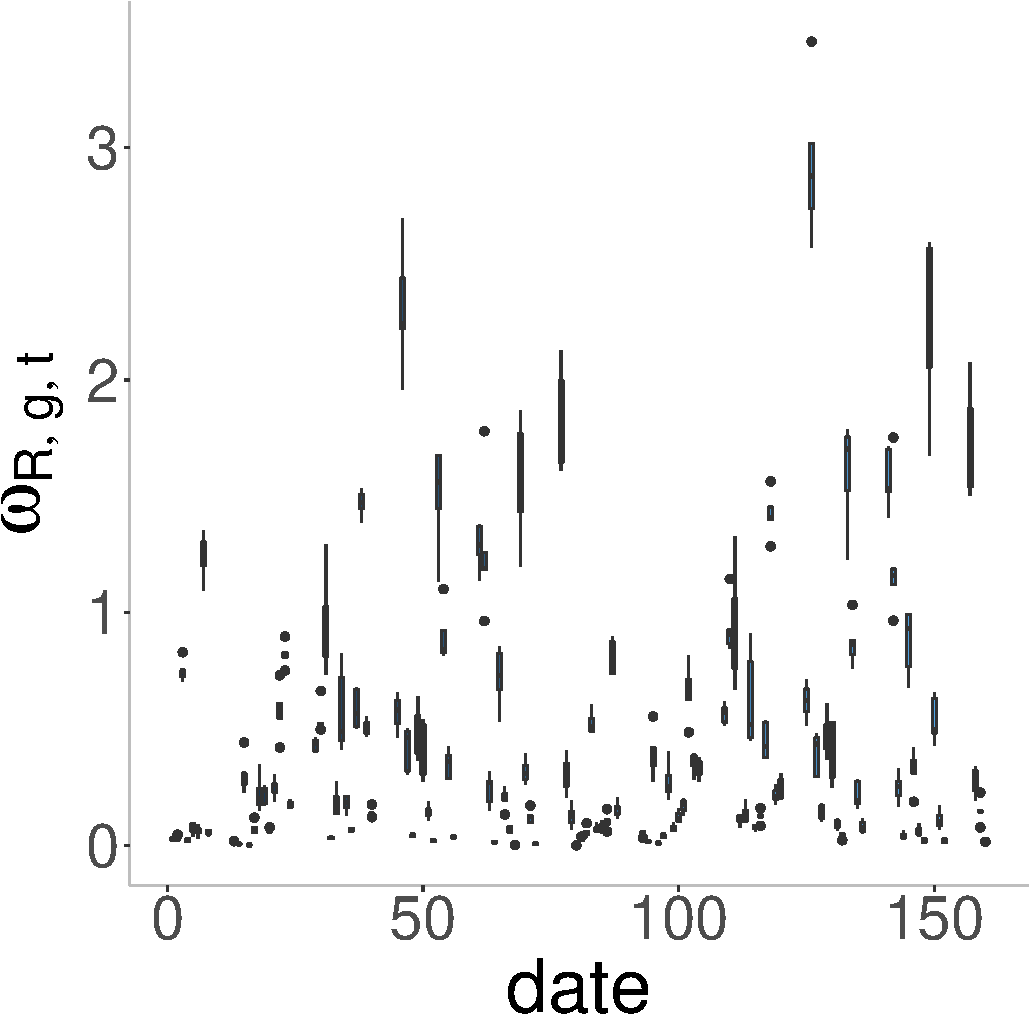
\includegraphics[width =5in, height =3in]{figs/weightsCPS78}
% Created by tikzDevice version 0.12.3.1 on 2023-11-03 10:48:14
% !TEX encoding = UTF-8 Unicode
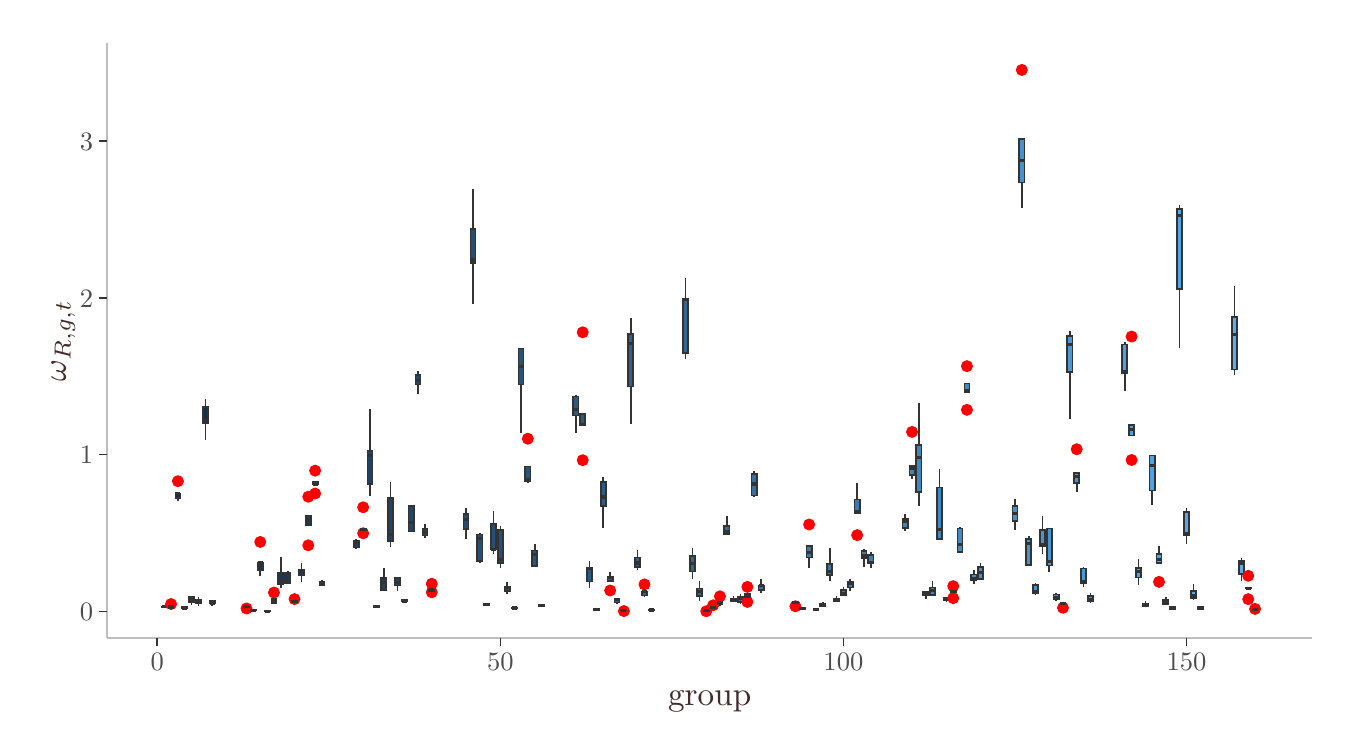
\begin{tikzpicture}[x=1pt,y=1pt]
\definecolor{fillColor}{RGB}{255,255,255}
\path[use as bounding box,fill=fillColor,fill opacity=0.00] (0,0) rectangle (469.75,252.94);
\begin{scope}
\path[clip] (  0.00,  0.00) rectangle (469.75,252.94);
\definecolor{drawColor}{RGB}{255,255,255}
\definecolor{fillColor}{RGB}{255,255,255}

\path[draw=drawColor,line width= 0.6pt,line join=round,line cap=round,fill=fillColor] (  0.00,  0.00) rectangle (469.76,252.94);
\end{scope}
\begin{scope}
\path[clip] ( 28.60, 32.28) rectangle (464.25,247.44);
\definecolor{drawColor}{RGB}{255,255,255}

\path[draw=drawColor,line width= 0.6pt,line join=round] ( 28.60, 42.02) --
	(464.25, 42.02);

\path[draw=drawColor,line width= 0.6pt,line join=round] ( 28.60, 98.66) --
	(464.25, 98.66);

\path[draw=drawColor,line width= 0.6pt,line join=round] ( 28.60,155.30) --
	(464.25,155.30);

\path[draw=drawColor,line width= 0.6pt,line join=round] ( 28.60,211.94) --
	(464.25,211.94);

\path[draw=drawColor,line width= 0.6pt,line join=round] ( 46.85, 32.28) --
	( 46.85,247.44);

\path[draw=drawColor,line width= 0.6pt,line join=round] (170.81, 32.28) --
	(170.81,247.44);

\path[draw=drawColor,line width= 0.6pt,line join=round] (294.77, 32.28) --
	(294.77,247.44);

\path[draw=drawColor,line width= 0.6pt,line join=round] (418.73, 32.28) --
	(418.73,247.44);
\definecolor{drawColor}{gray}{0.20}

\path[draw=drawColor,line width= 0.6pt,line join=round] ( 49.33, 43.82) -- ( 49.33, 44.17);

\path[draw=drawColor,line width= 0.6pt,line join=round] ( 49.33, 43.56) -- ( 49.33, 43.24);
\definecolor{fillColor}{RGB}{19,43,67}

\path[draw=drawColor,line width= 0.6pt,fill=fillColor] ( 48.40, 43.82) --
	( 48.40, 43.56) --
	( 50.26, 43.56) --
	( 50.26, 43.82) --
	( 48.40, 43.82) --
	cycle;

\path[draw=drawColor,line width= 1.1pt] ( 48.40, 43.62) -- ( 50.26, 43.62);
\definecolor{drawColor}{RGB}{255,0,0}
\definecolor{fillColor}{RGB}{255,0,0}

\path[draw=drawColor,line width= 0.4pt,line join=round,line cap=round,fill=fillColor] ( 51.81, 44.68) circle (  1.96);
\definecolor{drawColor}{gray}{0.20}

\path[draw=drawColor,line width= 0.6pt,line join=round] ( 51.81, 43.93) -- ( 51.81, 43.93);

\path[draw=drawColor,line width= 0.6pt,line join=round] ( 51.81, 43.46) -- ( 51.81, 43.08);
\definecolor{fillColor}{RGB}{19,44,68}

\path[draw=drawColor,line width= 0.6pt,fill=fillColor] ( 50.88, 43.93) --
	( 50.88, 43.46) --
	( 52.74, 43.46) --
	( 52.74, 43.93) --
	( 50.88, 43.93) --
	cycle;

\path[draw=drawColor,line width= 1.1pt] ( 50.88, 43.57) -- ( 52.74, 43.57);
\definecolor{drawColor}{RGB}{255,0,0}
\definecolor{fillColor}{RGB}{255,0,0}

\path[draw=drawColor,line width= 0.4pt,line join=round,line cap=round,fill=fillColor] ( 54.29, 89.06) circle (  1.96);
\definecolor{drawColor}{gray}{0.20}

\path[draw=drawColor,line width= 0.6pt,line join=round] ( 54.29, 84.51) -- ( 54.29, 84.51);

\path[draw=drawColor,line width= 0.6pt,line join=round] ( 54.29, 83.09) -- ( 54.29, 82.05);
\definecolor{fillColor}{RGB}{20,44,69}

\path[draw=drawColor,line width= 0.6pt,fill=fillColor] ( 53.36, 84.51) --
	( 53.36, 83.09) --
	( 55.22, 83.09) --
	( 55.22, 84.51) --
	( 53.36, 84.51) --
	cycle;

\path[draw=drawColor,line width= 1.1pt] ( 53.36, 84.46) -- ( 55.22, 84.46);

\path[draw=drawColor,line width= 0.6pt,line join=round] ( 56.77, 43.62) -- ( 56.77, 43.84);

\path[draw=drawColor,line width= 0.6pt,line join=round] ( 56.77, 43.00) -- ( 56.77, 42.97);
\definecolor{fillColor}{RGB}{20,45,70}

\path[draw=drawColor,line width= 0.6pt,fill=fillColor] ( 55.84, 43.62) --
	( 55.84, 43.00) --
	( 57.70, 43.00) --
	( 57.70, 43.62) --
	( 55.84, 43.62) --
	cycle;

\path[draw=drawColor,line width= 1.1pt] ( 55.84, 43.23) -- ( 57.70, 43.23);

\path[draw=drawColor,line width= 0.6pt,line join=round] ( 59.25, 47.27) -- ( 59.25, 47.51);

\path[draw=drawColor,line width= 0.6pt,line join=round] ( 59.25, 45.47) -- ( 59.25, 44.32);
\definecolor{fillColor}{RGB}{20,46,71}

\path[draw=drawColor,line width= 0.6pt,fill=fillColor] ( 58.32, 47.27) --
	( 58.32, 45.47) --
	( 60.18, 45.47) --
	( 60.18, 47.27) --
	( 58.32, 47.27) --
	cycle;

\path[draw=drawColor,line width= 1.1pt] ( 58.32, 46.40) -- ( 60.18, 46.40);

\path[draw=drawColor,line width= 0.6pt,line join=round] ( 61.72, 46.11) -- ( 61.72, 47.23);

\path[draw=drawColor,line width= 0.6pt,line join=round] ( 61.72, 45.12) -- ( 61.72, 43.83);
\definecolor{fillColor}{RGB}{21,47,72}

\path[draw=drawColor,line width= 0.6pt,fill=fillColor] ( 60.79, 46.11) --
	( 60.79, 45.12) --
	( 62.65, 45.12) --
	( 62.65, 46.11) --
	( 60.79, 46.11) --
	cycle;

\path[draw=drawColor,line width= 1.1pt] ( 60.79, 45.51) -- ( 62.65, 45.51);

\path[draw=drawColor,line width= 0.6pt,line join=round] ( 64.20,115.87) -- ( 64.20,118.59);

\path[draw=drawColor,line width= 0.6pt,line join=round] ( 64.20,110.16) -- ( 64.20,104.04);
\definecolor{fillColor}{RGB}{21,47,73}

\path[draw=drawColor,line width= 0.6pt,fill=fillColor] ( 63.27,115.87) --
	( 63.27,110.16) --
	( 65.13,110.16) --
	( 65.13,115.87) --
	( 63.27,115.87) --
	cycle;

\path[draw=drawColor,line width= 1.1pt] ( 63.27,111.08) -- ( 65.13,111.08);

\path[draw=drawColor,line width= 0.6pt,line join=round] ( 66.68, 45.66) -- ( 66.68, 45.72);

\path[draw=drawColor,line width= 0.6pt,line join=round] ( 66.68, 44.88) -- ( 66.68, 44.14);
\definecolor{fillColor}{RGB}{22,48,74}

\path[draw=drawColor,line width= 0.6pt,fill=fillColor] ( 65.75, 45.66) --
	( 65.75, 44.88) --
	( 67.61, 44.88) --
	( 67.61, 45.66) --
	( 65.75, 45.66) --
	cycle;

\path[draw=drawColor,line width= 1.1pt] ( 65.75, 45.02) -- ( 67.61, 45.02);
\definecolor{drawColor}{RGB}{255,0,0}
\definecolor{fillColor}{RGB}{255,0,0}

\path[draw=drawColor,line width= 0.4pt,line join=round,line cap=round,fill=fillColor] ( 79.08, 43.07) circle (  1.96);
\definecolor{drawColor}{gray}{0.20}

\path[draw=drawColor,line width= 0.6pt,line join=round] ( 79.08, 43.71) -- ( 79.08, 43.80);

\path[draw=drawColor,line width= 0.6pt,line join=round] ( 79.08, 43.60) -- ( 79.08, 43.60);
\definecolor{fillColor}{RGB}{24,52,79}

\path[draw=drawColor,line width= 0.6pt,fill=fillColor] ( 78.15, 43.71) --
	( 78.15, 43.60) --
	( 80.01, 43.60) --
	( 80.01, 43.71) --
	( 78.15, 43.71) --
	cycle;

\path[draw=drawColor,line width= 1.1pt] ( 78.15, 43.66) -- ( 80.01, 43.66);

\path[draw=drawColor,line width= 0.6pt,line join=round] ( 81.56, 42.49) -- ( 81.56, 42.62);

\path[draw=drawColor,line width= 0.6pt,line join=round] ( 81.56, 42.37) -- ( 81.56, 42.35);
\definecolor{fillColor}{RGB}{24,53,80}

\path[draw=drawColor,line width= 0.6pt,fill=fillColor] ( 80.63, 42.49) --
	( 80.63, 42.37) --
	( 82.49, 42.37) --
	( 82.49, 42.49) --
	( 80.63, 42.49) --
	cycle;

\path[draw=drawColor,line width= 1.1pt] ( 80.63, 42.42) -- ( 82.49, 42.42);
\definecolor{drawColor}{RGB}{255,0,0}
\definecolor{fillColor}{RGB}{255,0,0}

\path[draw=drawColor,line width= 0.4pt,line join=round,line cap=round,fill=fillColor] ( 84.04, 67.11) circle (  1.96);
\definecolor{drawColor}{gray}{0.20}

\path[draw=drawColor,line width= 0.6pt,line join=round] ( 84.04, 59.55) -- ( 84.04, 59.55);

\path[draw=drawColor,line width= 0.6pt,line join=round] ( 84.04, 56.90) -- ( 84.04, 54.95);
\definecolor{fillColor}{RGB}{24,53,81}

\path[draw=drawColor,line width= 0.6pt,fill=fillColor] ( 83.11, 59.55) --
	( 83.11, 56.90) --
	( 84.97, 56.90) --
	( 84.97, 59.55) --
	( 83.11, 59.55) --
	cycle;

\path[draw=drawColor,line width= 1.1pt] ( 83.11, 59.51) -- ( 84.97, 59.51);

\path[draw=drawColor,line width= 0.6pt,line join=round] ( 86.52, 42.15) -- ( 86.52, 42.19);

\path[draw=drawColor,line width= 0.6pt,line join=round] ( 86.52, 42.10) -- ( 86.52, 42.10);
\definecolor{fillColor}{RGB}{25,54,82}

\path[draw=drawColor,line width= 0.6pt,fill=fillColor] ( 85.59, 42.15) --
	( 85.59, 42.10) --
	( 87.45, 42.10) --
	( 87.45, 42.15) --
	( 85.59, 42.15) --
	cycle;

\path[draw=drawColor,line width= 1.1pt] ( 85.59, 42.13) -- ( 87.45, 42.13);
\definecolor{drawColor}{RGB}{255,0,0}
\definecolor{fillColor}{RGB}{255,0,0}

\path[draw=drawColor,line width= 0.4pt,line join=round,line cap=round,fill=fillColor] ( 89.00, 48.81) circle (  1.96);
\definecolor{drawColor}{gray}{0.20}

\path[draw=drawColor,line width= 0.6pt,line join=round] ( 89.00, 46.46) -- ( 89.00, 46.46);

\path[draw=drawColor,line width= 0.6pt,line join=round] ( 89.00, 45.13) -- ( 89.00, 44.85);
\definecolor{fillColor}{RGB}{25,55,83}

\path[draw=drawColor,line width= 0.6pt,fill=fillColor] ( 88.07, 46.46) --
	( 88.07, 45.13) --
	( 89.93, 45.13) --
	( 89.93, 46.46) --
	( 88.07, 46.46) --
	cycle;

\path[draw=drawColor,line width= 1.1pt] ( 88.07, 45.68) -- ( 89.93, 45.68);

\path[draw=drawColor,line width= 0.6pt,line join=round] ( 91.48, 55.94) -- ( 91.48, 61.73);

\path[draw=drawColor,line width= 0.6pt,line join=round] ( 91.48, 52.00) -- ( 91.48, 50.53);
\definecolor{fillColor}{RGB}{25,56,84}

\path[draw=drawColor,line width= 0.6pt,fill=fillColor] ( 90.55, 55.94) --
	( 90.55, 52.00) --
	( 92.40, 52.00) --
	( 92.40, 55.94) --
	( 90.55, 55.94) --
	cycle;

\path[draw=drawColor,line width= 1.1pt] ( 90.55, 53.29) -- ( 92.40, 53.29);

\path[draw=drawColor,line width= 0.6pt,line join=round] ( 93.95, 55.86) -- ( 93.95, 56.63);

\path[draw=drawColor,line width= 0.6pt,line join=round] ( 93.95, 52.19) -- ( 93.95, 51.80);
\definecolor{fillColor}{RGB}{26,56,85}

\path[draw=drawColor,line width= 0.6pt,fill=fillColor] ( 93.02, 55.86) --
	( 93.02, 52.19) --
	( 94.88, 52.19) --
	( 94.88, 55.86) --
	( 93.02, 55.86) --
	cycle;

\path[draw=drawColor,line width= 1.1pt] ( 93.02, 55.58) -- ( 94.88, 55.58);
\definecolor{drawColor}{RGB}{255,0,0}
\definecolor{fillColor}{RGB}{255,0,0}

\path[draw=drawColor,line width= 0.4pt,line join=round,line cap=round,fill=fillColor] ( 96.43, 46.45) circle (  1.96);
\definecolor{drawColor}{gray}{0.20}

\path[draw=drawColor,line width= 0.6pt,line join=round] ( 96.43, 45.65) -- ( 96.43, 45.65);

\path[draw=drawColor,line width= 0.6pt,line join=round] ( 96.43, 45.44) -- ( 96.43, 45.39);
\definecolor{fillColor}{RGB}{26,57,86}

\path[draw=drawColor,line width= 0.6pt,fill=fillColor] ( 95.50, 45.65) --
	( 95.50, 45.44) --
	( 97.36, 45.44) --
	( 97.36, 45.65) --
	( 95.50, 45.65) --
	cycle;

\path[draw=drawColor,line width= 1.1pt] ( 95.50, 45.58) -- ( 97.36, 45.58);

\path[draw=drawColor,line width= 0.6pt,line join=round] ( 98.91, 56.96) -- ( 98.91, 59.42);

\path[draw=drawColor,line width= 0.6pt,line join=round] ( 98.91, 54.98) -- ( 98.91, 52.73);
\definecolor{fillColor}{RGB}{27,58,87}

\path[draw=drawColor,line width= 0.6pt,fill=fillColor] ( 97.98, 56.96) --
	( 97.98, 54.98) --
	( 99.84, 54.98) --
	( 99.84, 56.96) --
	( 97.98, 56.96) --
	cycle;

\path[draw=drawColor,line width= 1.1pt] ( 97.98, 56.81) -- ( 99.84, 56.81);
\definecolor{drawColor}{RGB}{255,0,0}
\definecolor{fillColor}{RGB}{255,0,0}

\path[draw=drawColor,line width= 0.4pt,line join=round,line cap=round,fill=fillColor] (101.39, 65.89) circle (  1.96);

\path[draw=drawColor,line width= 0.4pt,line join=round,line cap=round,fill=fillColor] (101.39, 83.45) circle (  1.96);
\definecolor{drawColor}{gray}{0.20}

\path[draw=drawColor,line width= 0.6pt,line join=round] (101.39, 76.67) -- (101.39, 76.67);

\path[draw=drawColor,line width= 0.6pt,line join=round] (101.39, 73.07) -- (101.39, 73.07);
\definecolor{fillColor}{RGB}{27,59,88}

\path[draw=drawColor,line width= 0.6pt,fill=fillColor] (100.46, 76.67) --
	(100.46, 73.07) --
	(102.32, 73.07) --
	(102.32, 76.67) --
	(100.46, 76.67) --
	cycle;

\path[draw=drawColor,line width= 1.1pt] (100.46, 75.05) -- (102.32, 75.05);
\definecolor{drawColor}{RGB}{255,0,0}
\definecolor{fillColor}{RGB}{255,0,0}

\path[draw=drawColor,line width= 0.4pt,line join=round,line cap=round,fill=fillColor] (103.87, 92.86) circle (  1.96);

\path[draw=drawColor,line width= 0.4pt,line join=round,line cap=round,fill=fillColor] (103.87, 84.60) circle (  1.96);
\definecolor{drawColor}{gray}{0.20}

\path[draw=drawColor,line width= 0.6pt,line join=round] (103.87, 89.00) -- (103.87, 89.00);

\path[draw=drawColor,line width= 0.6pt,line join=round] (103.87, 87.83) -- (103.87, 87.83);
\definecolor{fillColor}{RGB}{27,60,89}

\path[draw=drawColor,line width= 0.6pt,fill=fillColor] (102.94, 89.00) --
	(102.94, 87.83) --
	(104.80, 87.83) --
	(104.80, 89.00) --
	(102.94, 89.00) --
	cycle;

\path[draw=drawColor,line width= 1.1pt] (102.94, 87.98) -- (104.80, 87.98);

\path[draw=drawColor,line width= 0.6pt,line join=round] (106.35, 52.56) -- (106.35, 53.33);

\path[draw=drawColor,line width= 0.6pt,line join=round] (106.35, 51.38) -- (106.35, 51.10);
\definecolor{fillColor}{RGB}{28,60,90}

\path[draw=drawColor,line width= 0.6pt,fill=fillColor] (105.42, 52.56) --
	(105.42, 51.38) --
	(107.28, 51.38) --
	(107.28, 52.56) --
	(105.42, 52.56) --
	cycle;

\path[draw=drawColor,line width= 1.1pt] (105.42, 51.57) -- (107.28, 51.57);

\path[draw=drawColor,line width= 0.6pt,line join=round] (118.75, 67.61) -- (118.75, 68.31);

\path[draw=drawColor,line width= 0.6pt,line join=round] (118.75, 65.05) -- (118.75, 64.64);
\definecolor{fillColor}{RGB}{30,64,96}

\path[draw=drawColor,line width= 0.6pt,fill=fillColor] (117.82, 67.61) --
	(117.82, 65.05) --
	(119.68, 65.05) --
	(119.68, 67.61) --
	(117.82, 67.61) --
	cycle;

\path[draw=drawColor,line width= 1.1pt] (117.82, 66.98) -- (119.68, 66.98);
\definecolor{drawColor}{RGB}{255,0,0}
\definecolor{fillColor}{RGB}{255,0,0}

\path[draw=drawColor,line width= 0.4pt,line join=round,line cap=round,fill=fillColor] (121.23, 79.63) circle (  1.96);

\path[draw=drawColor,line width= 0.4pt,line join=round,line cap=round,fill=fillColor] (121.23, 70.25) circle (  1.96);
\definecolor{drawColor}{gray}{0.20}

\path[draw=drawColor,line width= 0.6pt,line join=round] (121.23, 71.73) -- (121.23, 71.73);

\path[draw=drawColor,line width= 0.6pt,line join=round] (121.23, 71.30) -- (121.23, 71.30);
\definecolor{fillColor}{RGB}{30,65,97}

\path[draw=drawColor,line width= 0.6pt,fill=fillColor] (120.30, 71.73) --
	(120.30, 71.30) --
	(122.16, 71.30) --
	(122.16, 71.73) --
	(120.30, 71.73) --
	cycle;

\path[draw=drawColor,line width= 1.1pt] (120.30, 71.53) -- (122.16, 71.53);

\path[draw=drawColor,line width= 0.6pt,line join=round] (123.70,100.11) -- (123.70,115.24);

\path[draw=drawColor,line width= 0.6pt,line join=round] (123.70, 88.11) -- (123.70, 83.70);
\definecolor{fillColor}{RGB}{31,66,98}

\path[draw=drawColor,line width= 0.6pt,fill=fillColor] (122.78,100.11) --
	(122.78, 88.11) --
	(124.63, 88.11) --
	(124.63,100.11) --
	(122.78,100.11) --
	cycle;

\path[draw=drawColor,line width= 1.1pt] (122.78, 98.28) -- (124.63, 98.28);

\path[draw=drawColor,line width= 0.6pt,line join=round] (126.18, 44.04) -- (126.18, 44.06);

\path[draw=drawColor,line width= 0.6pt,line join=round] (126.18, 43.65) -- (126.18, 43.48);
\definecolor{fillColor}{RGB}{31,67,99}

\path[draw=drawColor,line width= 0.6pt,fill=fillColor] (125.25, 44.04) --
	(125.25, 43.65) --
	(127.11, 43.65) --
	(127.11, 44.04) --
	(125.25, 44.04) --
	cycle;

\path[draw=drawColor,line width= 1.1pt] (125.25, 43.93) -- (127.11, 43.93);

\path[draw=drawColor,line width= 0.6pt,line join=round] (128.66, 53.96) -- (128.66, 57.72);

\path[draw=drawColor,line width= 0.6pt,line join=round] (128.66, 49.79) -- (128.66, 49.57);
\definecolor{fillColor}{RGB}{31,67,100}

\path[draw=drawColor,line width= 0.6pt,fill=fillColor] (127.73, 53.96) --
	(127.73, 49.79) --
	(129.59, 49.79) --
	(129.59, 53.96) --
	(127.73, 53.96) --
	cycle;

\path[draw=drawColor,line width= 1.1pt] (127.73, 52.59) -- (129.59, 52.59);

\path[draw=drawColor,line width= 0.6pt,line join=round] (131.14, 82.92) -- (131.14, 88.76);

\path[draw=drawColor,line width= 0.6pt,line join=round] (131.14, 67.53) -- (131.14, 65.33);
\definecolor{fillColor}{RGB}{32,68,101}

\path[draw=drawColor,line width= 0.6pt,fill=fillColor] (130.21, 82.92) --
	(130.21, 67.53) --
	(132.07, 67.53) --
	(132.07, 82.92) --
	(130.21, 82.92) --
	cycle;

\path[draw=drawColor,line width= 1.1pt] (130.21, 69.72) -- (132.07, 69.72);

\path[draw=drawColor,line width= 0.6pt,line join=round] (133.62, 54.03) -- (133.62, 54.05);

\path[draw=drawColor,line width= 0.6pt,line join=round] (133.62, 51.31) -- (133.62, 49.34);
\definecolor{fillColor}{RGB}{32,69,102}

\path[draw=drawColor,line width= 0.6pt,fill=fillColor] (132.69, 54.03) --
	(132.69, 51.31) --
	(134.55, 51.31) --
	(134.55, 54.03) --
	(132.69, 54.03) --
	cycle;

\path[draw=drawColor,line width= 1.1pt] (132.69, 52.46) -- (134.55, 52.46);

\path[draw=drawColor,line width= 0.6pt,line join=round] (136.10, 46.17) -- (136.10, 46.23);

\path[draw=drawColor,line width= 0.6pt,line join=round] (136.10, 45.53) -- (136.10, 45.18);
\definecolor{fillColor}{RGB}{33,70,103}

\path[draw=drawColor,line width= 0.6pt,fill=fillColor] (135.17, 46.17) --
	(135.17, 45.53) --
	(137.03, 45.53) --
	(137.03, 46.17) --
	(135.17, 46.17) --
	cycle;

\path[draw=drawColor,line width= 1.1pt] (135.17, 45.69) -- (137.03, 45.69);

\path[draw=drawColor,line width= 0.6pt,line join=round] (138.58, 80.02) -- (138.58, 80.47);

\path[draw=drawColor,line width= 0.6pt,line join=round] (138.58, 70.94) -- (138.58, 70.58);
\definecolor{fillColor}{RGB}{33,70,104}

\path[draw=drawColor,line width= 0.6pt,fill=fillColor] (137.65, 80.02) --
	(137.65, 70.94) --
	(139.51, 70.94) --
	(139.51, 80.02) --
	(137.65, 80.02) --
	cycle;

\path[draw=drawColor,line width= 1.1pt] (137.65, 74.10) -- (139.51, 74.10);

\path[draw=drawColor,line width= 0.6pt,line join=round] (141.06,127.43) -- (141.06,129.00);

\path[draw=drawColor,line width= 0.6pt,line join=round] (141.06,124.00) -- (141.06,120.59);
\definecolor{fillColor}{RGB}{33,71,105}

\path[draw=drawColor,line width= 0.6pt,fill=fillColor] (140.13,127.43) --
	(140.13,124.00) --
	(141.99,124.00) --
	(141.99,127.43) --
	(140.13,127.43) --
	cycle;

\path[draw=drawColor,line width= 1.1pt] (140.13,125.53) -- (141.99,125.53);

\path[draw=drawColor,line width= 0.6pt,line join=round] (143.54, 71.85) -- (143.54, 73.54);

\path[draw=drawColor,line width= 0.6pt,line join=round] (143.54, 69.39) -- (143.54, 68.53);
\definecolor{fillColor}{RGB}{34,72,106}

\path[draw=drawColor,line width= 0.6pt,fill=fillColor] (142.61, 71.85) --
	(142.61, 69.39) --
	(144.47, 69.39) --
	(144.47, 71.85) --
	(142.61, 71.85) --
	cycle;

\path[draw=drawColor,line width= 1.1pt] (142.61, 70.64) -- (144.47, 70.64);
\definecolor{drawColor}{RGB}{255,0,0}
\definecolor{fillColor}{RGB}{255,0,0}

\path[draw=drawColor,line width= 0.4pt,line join=round,line cap=round,fill=fillColor] (146.02, 51.99) circle (  1.96);

\path[draw=drawColor,line width= 0.4pt,line join=round,line cap=round,fill=fillColor] (146.02, 48.91) circle (  1.96);
\definecolor{drawColor}{gray}{0.20}

\path[draw=drawColor,line width= 0.6pt,line join=round] (146.02, 49.87) -- (146.02, 49.87);

\path[draw=drawColor,line width= 0.6pt,line join=round] (146.02, 49.49) -- (146.02, 49.49);
\definecolor{fillColor}{RGB}{34,73,107}

\path[draw=drawColor,line width= 0.6pt,fill=fillColor] (145.09, 49.87) --
	(145.09, 49.49) --
	(146.95, 49.49) --
	(146.95, 49.87) --
	(145.09, 49.87) --
	cycle;

\path[draw=drawColor,line width= 1.1pt] (145.09, 49.82) -- (146.95, 49.82);

\path[draw=drawColor,line width= 0.6pt,line join=round] (158.41, 77.23) -- (158.41, 79.22);

\path[draw=drawColor,line width= 0.6pt,line join=round] (158.41, 71.77) -- (158.41, 68.23);
\definecolor{fillColor}{RGB}{36,77,113}

\path[draw=drawColor,line width= 0.6pt,fill=fillColor] (157.48, 77.23) --
	(157.48, 71.77) --
	(159.34, 71.77) --
	(159.34, 77.23) --
	(157.48, 77.23) --
	cycle;

\path[draw=drawColor,line width= 1.1pt] (157.48, 75.05) -- (159.34, 75.05);

\path[draw=drawColor,line width= 0.6pt,line join=round] (160.89,180.14) -- (160.89,194.56);

\path[draw=drawColor,line width= 0.6pt,line join=round] (160.89,167.79) -- (160.89,152.96);
\definecolor{fillColor}{RGB}{37,78,114}

\path[draw=drawColor,line width= 0.6pt,fill=fillColor] (159.96,180.14) --
	(159.96,167.79) --
	(161.82,167.79) --
	(161.82,180.14) --
	(159.96,180.14) --
	cycle;

\path[draw=drawColor,line width= 1.1pt] (159.96,168.98) -- (161.82,168.98);

\path[draw=drawColor,line width= 0.6pt,line join=round] (163.37, 69.75) -- (163.37, 70.42);

\path[draw=drawColor,line width= 0.6pt,line join=round] (163.37, 60.17) -- (163.37, 59.41);
\definecolor{fillColor}{RGB}{37,78,115}

\path[draw=drawColor,line width= 0.6pt,fill=fillColor] (162.44, 69.75) --
	(162.44, 60.17) --
	(164.30, 60.17) --
	(164.30, 69.75) --
	(162.44, 69.75) --
	cycle;

\path[draw=drawColor,line width= 1.1pt] (162.44, 68.26) -- (164.30, 68.26);

\path[draw=drawColor,line width= 0.6pt,line join=round] (165.85, 44.65) -- (165.85, 44.94);

\path[draw=drawColor,line width= 0.6pt,line join=round] (165.85, 44.23) -- (165.85, 43.98);
\definecolor{fillColor}{RGB}{37,79,116}

\path[draw=drawColor,line width= 0.6pt,fill=fillColor] (164.92, 44.65) --
	(164.92, 44.23) --
	(166.78, 44.23) --
	(166.78, 44.65) --
	(164.92, 44.65) --
	cycle;

\path[draw=drawColor,line width= 1.1pt] (164.92, 44.61) -- (166.78, 44.61);

\path[draw=drawColor,line width= 0.6pt,line join=round] (168.33, 73.57) -- (168.33, 78.30);

\path[draw=drawColor,line width= 0.6pt,line join=round] (168.33, 64.52) -- (168.33, 62.63);
\definecolor{fillColor}{RGB}{38,80,117}

\path[draw=drawColor,line width= 0.6pt,fill=fillColor] (167.40, 73.57) --
	(167.40, 64.52) --
	(169.26, 64.52) --
	(169.26, 73.57) --
	(167.40, 73.57) --
	cycle;

\path[draw=drawColor,line width= 1.1pt] (167.40, 64.52) -- (169.26, 64.52);

\path[draw=drawColor,line width= 0.6pt,line join=round] (170.81, 71.40) -- (170.81, 72.80);

\path[draw=drawColor,line width= 0.6pt,line join=round] (170.81, 59.40) -- (170.81, 57.70);
\definecolor{fillColor}{RGB}{38,81,118}

\path[draw=drawColor,line width= 0.6pt,fill=fillColor] (169.88, 71.40) --
	(169.88, 59.40) --
	(171.74, 59.40) --
	(171.74, 71.40) --
	(169.88, 71.40) --
	cycle;

\path[draw=drawColor,line width= 1.1pt] (169.88, 60.82) -- (171.74, 60.82);

\path[draw=drawColor,line width= 0.6pt,line join=round] (173.29, 50.79) -- (173.29, 52.68);

\path[draw=drawColor,line width= 0.6pt,line join=round] (173.29, 49.38) -- (173.29, 48.15);
\definecolor{fillColor}{RGB}{39,82,119}

\path[draw=drawColor,line width= 0.6pt,fill=fillColor] (172.36, 50.79) --
	(172.36, 49.38) --
	(174.22, 49.38) --
	(174.22, 50.79) --
	(172.36, 50.79) --
	cycle;

\path[draw=drawColor,line width= 1.1pt] (172.36, 50.65) -- (174.22, 50.65);

\path[draw=drawColor,line width= 0.6pt,line join=round] (175.77, 43.37) -- (175.77, 43.43);

\path[draw=drawColor,line width= 0.6pt,line join=round] (175.77, 43.03) -- (175.77, 42.79);
\definecolor{fillColor}{RGB}{39,82,120}

\path[draw=drawColor,line width= 0.6pt,fill=fillColor] (174.84, 43.37) --
	(174.84, 43.03) --
	(176.70, 43.03) --
	(176.70, 43.37) --
	(174.84, 43.37) --
	cycle;

\path[draw=drawColor,line width= 1.1pt] (174.84, 43.24) -- (176.70, 43.24);

\path[draw=drawColor,line width= 0.6pt,line join=round] (178.25,136.95) -- (178.25,137.02);

\path[draw=drawColor,line width= 0.6pt,line join=round] (178.25,123.99) -- (178.25,106.31);
\definecolor{fillColor}{RGB}{39,83,121}

\path[draw=drawColor,line width= 0.6pt,fill=fillColor] (177.32,136.95) --
	(177.32,123.99) --
	(179.18,123.99) --
	(179.18,136.95) --
	(177.32,136.95) --
	cycle;

\path[draw=drawColor,line width= 1.1pt] (177.32,130.45) -- (179.18,130.45);
\definecolor{drawColor}{RGB}{255,0,0}
\definecolor{fillColor}{RGB}{255,0,0}

\path[draw=drawColor,line width= 0.4pt,line join=round,line cap=round,fill=fillColor] (180.73,104.41) circle (  1.96);
\definecolor{drawColor}{gray}{0.20}

\path[draw=drawColor,line width= 0.6pt,line join=round] (180.73, 94.34) -- (180.73, 94.34);

\path[draw=drawColor,line width= 0.6pt,line join=round] (180.73, 88.93) -- (180.73, 88.31);
\definecolor{fillColor}{RGB}{40,84,122}

\path[draw=drawColor,line width= 0.6pt,fill=fillColor] (179.80, 94.34) --
	(179.80, 88.93) --
	(181.66, 88.93) --
	(181.66, 94.34) --
	(179.80, 94.34) --
	cycle;

\path[draw=drawColor,line width= 1.1pt] (179.80, 89.59) -- (181.66, 89.59);

\path[draw=drawColor,line width= 0.6pt,line join=round] (183.21, 63.98) -- (183.21, 66.23);

\path[draw=drawColor,line width= 0.6pt,line join=round] (183.21, 58.32) -- (183.21, 58.19);
\definecolor{fillColor}{RGB}{40,85,123}

\path[draw=drawColor,line width= 0.6pt,fill=fillColor] (182.28, 63.98) --
	(182.28, 58.32) --
	(184.14, 58.32) --
	(184.14, 63.98) --
	(182.28, 63.98) --
	cycle;

\path[draw=drawColor,line width= 1.1pt] (182.28, 62.52) -- (184.14, 62.52);

\path[draw=drawColor,line width= 0.6pt,line join=round] (185.69, 44.25) -- (185.69, 44.30);

\path[draw=drawColor,line width= 0.6pt,line join=round] (185.69, 44.03) -- (185.69, 43.70);
\definecolor{fillColor}{RGB}{41,86,125}

\path[draw=drawColor,line width= 0.6pt,fill=fillColor] (184.76, 44.25) --
	(184.76, 44.03) --
	(186.61, 44.03) --
	(186.61, 44.25) --
	(184.76, 44.25) --
	cycle;

\path[draw=drawColor,line width= 1.1pt] (184.76, 44.09) -- (186.61, 44.09);

\path[draw=drawColor,line width= 0.6pt,line join=round] (198.08,119.70) -- (198.08,120.06);

\path[draw=drawColor,line width= 0.6pt,line join=round] (198.08,112.77) -- (198.08,106.53);
\definecolor{fillColor}{RGB}{43,90,130}

\path[draw=drawColor,line width= 0.6pt,fill=fillColor] (197.15,119.70) --
	(197.15,112.77) --
	(199.01,112.77) --
	(199.01,119.70) --
	(197.15,119.70) --
	cycle;

\path[draw=drawColor,line width= 1.1pt] (197.15,115.13) -- (199.01,115.13);
\definecolor{drawColor}{RGB}{255,0,0}
\definecolor{fillColor}{RGB}{255,0,0}

\path[draw=drawColor,line width= 0.4pt,line join=round,line cap=round,fill=fillColor] (200.56,142.86) circle (  1.96);

\path[draw=drawColor,line width= 0.4pt,line join=round,line cap=round,fill=fillColor] (200.56, 96.65) circle (  1.96);
\definecolor{drawColor}{gray}{0.20}

\path[draw=drawColor,line width= 0.6pt,line join=round] (200.56,113.34) -- (200.56,113.34);

\path[draw=drawColor,line width= 0.6pt,line join=round] (200.56,109.27) -- (200.56,109.27);
\definecolor{fillColor}{RGB}{43,91,131}

\path[draw=drawColor,line width= 0.6pt,fill=fillColor] (199.63,113.34) --
	(199.63,109.27) --
	(201.49,109.27) --
	(201.49,113.34) --
	(199.63,113.34) --
	cycle;

\path[draw=drawColor,line width= 1.1pt] (199.63,109.48) -- (201.49,109.48);

\path[draw=drawColor,line width= 0.6pt,line join=round] (203.04, 57.62) -- (203.04, 60.15);

\path[draw=drawColor,line width= 0.6pt,line join=round] (203.04, 52.83) -- (203.04, 50.44);
\definecolor{fillColor}{RGB}{43,91,132}

\path[draw=drawColor,line width= 0.6pt,fill=fillColor] (202.11, 57.62) --
	(202.11, 52.83) --
	(203.97, 52.83) --
	(203.97, 57.62) --
	(202.11, 57.62) --
	cycle;

\path[draw=drawColor,line width= 1.1pt] (202.11, 57.35) -- (203.97, 57.35);

\path[draw=drawColor,line width= 0.6pt,line join=round] (205.52, 42.92) -- (205.52, 42.96);

\path[draw=drawColor,line width= 0.6pt,line join=round] (205.52, 42.63) -- (205.52, 42.35);
\definecolor{fillColor}{RGB}{44,92,133}

\path[draw=drawColor,line width= 0.6pt,fill=fillColor] (204.59, 42.92) --
	(204.59, 42.63) --
	(206.45, 42.63) --
	(206.45, 42.92) --
	(204.59, 42.92) --
	cycle;

\path[draw=drawColor,line width= 1.1pt] (204.59, 42.75) -- (206.45, 42.75);

\path[draw=drawColor,line width= 0.6pt,line join=round] (208.00, 88.77) -- (208.00, 90.42);

\path[draw=drawColor,line width= 0.6pt,line join=round] (208.00, 80.05) -- (208.00, 72.13);
\definecolor{fillColor}{RGB}{44,93,134}

\path[draw=drawColor,line width= 0.6pt,fill=fillColor] (207.07, 88.77) --
	(207.07, 80.05) --
	(208.93, 80.05) --
	(208.93, 88.77) --
	(207.07, 88.77) --
	cycle;

\path[draw=drawColor,line width= 1.1pt] (207.07, 83.34) -- (208.93, 83.34);
\definecolor{drawColor}{RGB}{255,0,0}
\definecolor{fillColor}{RGB}{255,0,0}

\path[draw=drawColor,line width= 0.4pt,line join=round,line cap=round,fill=fillColor] (210.48, 49.57) circle (  1.96);
\definecolor{drawColor}{gray}{0.20}

\path[draw=drawColor,line width= 0.6pt,line join=round] (210.48, 54.62) -- (210.48, 56.35);

\path[draw=drawColor,line width= 0.6pt,line join=round] (210.48, 53.07) -- (210.48, 53.07);
\definecolor{fillColor}{RGB}{45,94,136}

\path[draw=drawColor,line width= 0.6pt,fill=fillColor] (209.55, 54.62) --
	(209.55, 53.07) --
	(211.41, 53.07) --
	(211.41, 54.62) --
	(209.55, 54.62) --
	cycle;

\path[draw=drawColor,line width= 1.1pt] (209.55, 54.42) -- (211.41, 54.42);

\path[draw=drawColor,line width= 0.6pt,line join=round] (212.96, 46.58) -- (212.96, 46.66);

\path[draw=drawColor,line width= 0.6pt,line join=round] (212.96, 45.21) -- (212.96, 45.07);
\definecolor{fillColor}{RGB}{45,95,137}

\path[draw=drawColor,line width= 0.6pt,fill=fillColor] (212.03, 46.58) --
	(212.03, 45.21) --
	(213.89, 45.21) --
	(213.89, 46.58) --
	(212.03, 46.58) --
	cycle;

\path[draw=drawColor,line width= 1.1pt] (212.03, 46.18) -- (213.89, 46.18);
\definecolor{drawColor}{RGB}{255,0,0}
\definecolor{fillColor}{RGB}{255,0,0}

\path[draw=drawColor,line width= 0.4pt,line join=round,line cap=round,fill=fillColor] (215.44, 42.12) circle (  1.96);
\definecolor{drawColor}{gray}{0.20}

\path[draw=drawColor,line width= 0.6pt,line join=round] (215.44, 42.37) -- (215.44, 42.38);

\path[draw=drawColor,line width= 0.6pt,line join=round] (215.44, 42.33) -- (215.44, 42.33);
\definecolor{fillColor}{RGB}{46,96,138}

\path[draw=drawColor,line width= 0.6pt,fill=fillColor] (214.51, 42.37) --
	(214.51, 42.33) --
	(216.37, 42.33) --
	(216.37, 42.37) --
	(214.51, 42.37) --
	cycle;

\path[draw=drawColor,line width= 1.1pt] (214.51, 42.34) -- (216.37, 42.34);

\path[draw=drawColor,line width= 0.6pt,line join=round] (217.91,142.25) -- (217.91,147.93);

\path[draw=drawColor,line width= 0.6pt,line join=round] (217.91,123.24) -- (217.91,109.88);
\definecolor{fillColor}{RGB}{46,96,139}

\path[draw=drawColor,line width= 0.6pt,fill=fillColor] (216.99,142.25) --
	(216.99,123.24) --
	(218.84,123.24) --
	(218.84,142.25) --
	(216.99,142.25) --
	cycle;

\path[draw=drawColor,line width= 1.1pt] (216.99,138.70) -- (218.84,138.70);

\path[draw=drawColor,line width= 0.6pt,line join=round] (220.39, 61.51) -- (220.39, 64.34);

\path[draw=drawColor,line width= 0.6pt,line join=round] (220.39, 58.17) -- (220.39, 56.84);
\definecolor{fillColor}{RGB}{46,97,140}

\path[draw=drawColor,line width= 0.6pt,fill=fillColor] (219.46, 61.51) --
	(219.46, 58.17) --
	(221.32, 58.17) --
	(221.32, 61.51) --
	(219.46, 61.51) --
	cycle;

\path[draw=drawColor,line width= 1.1pt] (219.46, 59.50) -- (221.32, 59.50);
\definecolor{drawColor}{RGB}{255,0,0}
\definecolor{fillColor}{RGB}{255,0,0}

\path[draw=drawColor,line width= 0.4pt,line join=round,line cap=round,fill=fillColor] (222.87, 51.76) circle (  1.96);
\definecolor{drawColor}{gray}{0.20}

\path[draw=drawColor,line width= 0.6pt,line join=round] (222.87, 49.23) -- (222.87, 49.23);

\path[draw=drawColor,line width= 0.6pt,line join=round] (222.87, 47.70) -- (222.87, 47.54);
\definecolor{fillColor}{RGB}{47,98,141}

\path[draw=drawColor,line width= 0.6pt,fill=fillColor] (221.94, 49.23) --
	(221.94, 47.70) --
	(223.80, 47.70) --
	(223.80, 49.23) --
	(221.94, 49.23) --
	cycle;

\path[draw=drawColor,line width= 1.1pt] (221.94, 49.09) -- (223.80, 49.09);

\path[draw=drawColor,line width= 0.6pt,line join=round] (225.35, 42.57) -- (225.35, 42.58);

\path[draw=drawColor,line width= 0.6pt,line join=round] (225.35, 42.33) -- (225.35, 42.29);
\definecolor{fillColor}{RGB}{47,99,142}

\path[draw=drawColor,line width= 0.6pt,fill=fillColor] (224.42, 42.57) --
	(224.42, 42.33) --
	(226.28, 42.33) --
	(226.28, 42.57) --
	(224.42, 42.57) --
	cycle;

\path[draw=drawColor,line width= 1.1pt] (224.42, 42.52) -- (226.28, 42.52);

\path[draw=drawColor,line width= 0.6pt,line join=round] (237.75,155.09) -- (237.75,162.58);

\path[draw=drawColor,line width= 0.6pt,line join=round] (237.75,135.30) -- (237.75,133.26);
\definecolor{fillColor}{RGB}{49,103,148}

\path[draw=drawColor,line width= 0.6pt,fill=fillColor] (236.82,155.09) --
	(236.82,135.30) --
	(238.68,135.30) --
	(238.68,155.09) --
	(236.82,155.09) --
	cycle;

\path[draw=drawColor,line width= 1.1pt] (236.82,154.70) -- (238.68,154.70);

\path[draw=drawColor,line width= 0.6pt,line join=round] (240.23, 62.08) -- (240.23, 65.04);

\path[draw=drawColor,line width= 0.6pt,line join=round] (240.23, 56.44) -- (240.23, 53.81);
\definecolor{fillColor}{RGB}{50,104,149}

\path[draw=drawColor,line width= 0.6pt,fill=fillColor] (239.30, 62.08) --
	(239.30, 56.44) --
	(241.16, 56.44) --
	(241.16, 62.08) --
	(239.30, 62.08) --
	cycle;

\path[draw=drawColor,line width= 1.1pt] (239.30, 59.33) -- (241.16, 59.33);

\path[draw=drawColor,line width= 0.6pt,line join=round] (242.71, 50.30) -- (242.71, 52.90);

\path[draw=drawColor,line width= 0.6pt,line join=round] (242.71, 47.63) -- (242.71, 45.87);
\definecolor{fillColor}{RGB}{50,105,150}

\path[draw=drawColor,line width= 0.6pt,fill=fillColor] (241.78, 50.30) --
	(241.78, 47.63) --
	(243.64, 47.63) --
	(243.64, 50.30) --
	(241.78, 50.30) --
	cycle;

\path[draw=drawColor,line width= 1.1pt] (241.78, 49.18) -- (243.64, 49.18);
\definecolor{drawColor}{RGB}{255,0,0}
\definecolor{fillColor}{RGB}{255,0,0}

\path[draw=drawColor,line width= 0.4pt,line join=round,line cap=round,fill=fillColor] (245.19, 42.06) circle (  1.96);
\definecolor{drawColor}{gray}{0.20}

\path[draw=drawColor,line width= 0.6pt,line join=round] (245.19, 42.24) -- (245.19, 42.26);

\path[draw=drawColor,line width= 0.6pt,line join=round] (245.19, 42.19) -- (245.19, 42.19);
\definecolor{fillColor}{RGB}{51,106,151}

\path[draw=drawColor,line width= 0.6pt,fill=fillColor] (244.26, 42.24) --
	(244.26, 42.19) --
	(246.12, 42.19) --
	(246.12, 42.24) --
	(244.26, 42.24) --
	cycle;

\path[draw=drawColor,line width= 1.1pt] (244.26, 42.21) -- (246.12, 42.21);
\definecolor{drawColor}{RGB}{255,0,0}
\definecolor{fillColor}{RGB}{255,0,0}

\path[draw=drawColor,line width= 0.4pt,line join=round,line cap=round,fill=fillColor] (247.67, 44.21) circle (  1.96);
\definecolor{drawColor}{gray}{0.20}

\path[draw=drawColor,line width= 0.6pt,line join=round] (247.67, 43.54) -- (247.67, 43.54);

\path[draw=drawColor,line width= 0.6pt,line join=round] (247.67, 43.22) -- (247.67, 43.16);
\definecolor{fillColor}{RGB}{51,107,153}

\path[draw=drawColor,line width= 0.6pt,fill=fillColor] (246.74, 43.54) --
	(246.74, 43.22) --
	(248.59, 43.22) --
	(248.59, 43.54) --
	(246.74, 43.54) --
	cycle;

\path[draw=drawColor,line width= 1.1pt] (246.74, 43.50) -- (248.59, 43.50);
\definecolor{drawColor}{RGB}{255,0,0}
\definecolor{fillColor}{RGB}{255,0,0}

\path[draw=drawColor,line width= 0.4pt,line join=round,line cap=round,fill=fillColor] (250.14, 47.46) circle (  1.96);
\definecolor{drawColor}{gray}{0.20}

\path[draw=drawColor,line width= 0.6pt,line join=round] (250.14, 45.53) -- (250.14, 45.53);

\path[draw=drawColor,line width= 0.6pt,line join=round] (250.14, 44.71) -- (250.14, 44.06);
\definecolor{fillColor}{RGB}{51,107,154}

\path[draw=drawColor,line width= 0.6pt,fill=fillColor] (249.21, 45.53) --
	(249.21, 44.71) --
	(251.07, 44.71) --
	(251.07, 45.53) --
	(249.21, 45.53) --
	cycle;

\path[draw=drawColor,line width= 1.1pt] (249.21, 45.25) -- (251.07, 45.25);

\path[draw=drawColor,line width= 0.6pt,line join=round] (252.62, 72.92) -- (252.62, 76.36);

\path[draw=drawColor,line width= 0.6pt,line join=round] (252.62, 69.89) -- (252.62, 69.45);
\definecolor{fillColor}{RGB}{52,108,155}

\path[draw=drawColor,line width= 0.6pt,fill=fillColor] (251.69, 72.92) --
	(251.69, 69.89) --
	(253.55, 69.89) --
	(253.55, 72.92) --
	(251.69, 72.92) --
	cycle;

\path[draw=drawColor,line width= 1.1pt] (251.69, 70.84) -- (253.55, 70.84);

\path[draw=drawColor,line width= 0.6pt,line join=round] (255.10, 46.38) -- (255.10, 47.55);

\path[draw=drawColor,line width= 0.6pt,line join=round] (255.10, 45.60) -- (255.10, 45.27);
\definecolor{fillColor}{RGB}{52,109,156}

\path[draw=drawColor,line width= 0.6pt,fill=fillColor] (254.17, 46.38) --
	(254.17, 45.60) --
	(256.03, 45.60) --
	(256.03, 46.38) --
	(254.17, 46.38) --
	cycle;

\path[draw=drawColor,line width= 1.1pt] (254.17, 45.79) -- (256.03, 45.79);

\path[draw=drawColor,line width= 0.6pt,line join=round] (257.58, 47.17) -- (257.58, 48.22);

\path[draw=drawColor,line width= 0.6pt,line join=round] (257.58, 45.36) -- (257.58, 44.85);
\definecolor{fillColor}{RGB}{53,110,157}

\path[draw=drawColor,line width= 0.6pt,fill=fillColor] (256.65, 47.17) --
	(256.65, 45.36) --
	(258.51, 45.36) --
	(258.51, 47.17) --
	(256.65, 47.17) --
	cycle;

\path[draw=drawColor,line width= 1.1pt] (256.65, 46.74) -- (258.51, 46.74);
\definecolor{drawColor}{RGB}{255,0,0}
\definecolor{fillColor}{RGB}{255,0,0}

\path[draw=drawColor,line width= 0.4pt,line join=round,line cap=round,fill=fillColor] (260.06, 45.44) circle (  1.96);

\path[draw=drawColor,line width= 0.4pt,line join=round,line cap=round,fill=fillColor] (260.06, 50.87) circle (  1.96);
\definecolor{drawColor}{gray}{0.20}

\path[draw=drawColor,line width= 0.6pt,line join=round] (260.06, 48.37) -- (260.06, 48.37);

\path[draw=drawColor,line width= 0.6pt,line join=round] (260.06, 47.26) -- (260.06, 47.26);
\definecolor{fillColor}{RGB}{53,111,158}

\path[draw=drawColor,line width= 0.6pt,fill=fillColor] (259.13, 48.37) --
	(259.13, 47.26) --
	(260.99, 47.26) --
	(260.99, 48.37) --
	(259.13, 48.37) --
	cycle;

\path[draw=drawColor,line width= 1.1pt] (259.13, 47.68) -- (260.99, 47.68);

\path[draw=drawColor,line width= 0.6pt,line join=round] (262.54, 91.56) -- (262.54, 92.87);

\path[draw=drawColor,line width= 0.6pt,line join=round] (262.54, 83.88) -- (262.54, 83.62);
\definecolor{fillColor}{RGB}{54,112,159}

\path[draw=drawColor,line width= 0.6pt,fill=fillColor] (261.61, 91.56) --
	(261.61, 83.88) --
	(263.47, 83.88) --
	(263.47, 91.56) --
	(261.61, 91.56) --
	cycle;

\path[draw=drawColor,line width= 1.1pt] (261.61, 88.05) -- (263.47, 88.05);

\path[draw=drawColor,line width= 0.6pt,line join=round] (265.02, 51.42) -- (265.02, 53.82);

\path[draw=drawColor,line width= 0.6pt,line join=round] (265.02, 49.69) -- (265.02, 48.61);
\definecolor{fillColor}{RGB}{54,113,161}

\path[draw=drawColor,line width= 0.6pt,fill=fillColor] (264.09, 51.42) --
	(264.09, 49.69) --
	(265.95, 49.69) --
	(265.95, 51.42) --
	(264.09, 51.42) --
	cycle;

\path[draw=drawColor,line width= 1.1pt] (264.09, 51.33) -- (265.95, 51.33);
\definecolor{drawColor}{RGB}{255,0,0}
\definecolor{fillColor}{RGB}{255,0,0}

\path[draw=drawColor,line width= 0.4pt,line join=round,line cap=round,fill=fillColor] (277.42, 43.86) circle (  1.96);
\definecolor{drawColor}{gray}{0.20}

\path[draw=drawColor,line width= 0.6pt,line join=round] (277.42, 45.35) -- (277.42, 45.38);

\path[draw=drawColor,line width= 0.6pt,line join=round] (277.42, 44.82) -- (277.42, 44.82);
\definecolor{fillColor}{RGB}{56,117,166}

\path[draw=drawColor,line width= 0.6pt,fill=fillColor] (276.49, 45.35) --
	(276.49, 44.82) --
	(278.35, 44.82) --
	(278.35, 45.35) --
	(276.49, 45.35) --
	cycle;

\path[draw=drawColor,line width= 1.1pt] (276.49, 45.12) -- (278.35, 45.12);

\path[draw=drawColor,line width= 0.6pt,line join=round] (279.89, 43.14) -- (279.89, 43.21);

\path[draw=drawColor,line width= 0.6pt,line join=round] (279.89, 42.87) -- (279.89, 42.79);
\definecolor{fillColor}{RGB}{57,118,167}

\path[draw=drawColor,line width= 0.6pt,fill=fillColor] (278.97, 43.14) --
	(278.97, 42.87) --
	(280.82, 42.87) --
	(280.82, 43.14) --
	(278.97, 43.14) --
	cycle;

\path[draw=drawColor,line width= 1.1pt] (278.97, 43.06) -- (280.82, 43.06);
\definecolor{drawColor}{RGB}{255,0,0}
\definecolor{fillColor}{RGB}{255,0,0}

\path[draw=drawColor,line width= 0.4pt,line join=round,line cap=round,fill=fillColor] (282.37, 73.41) circle (  1.96);
\definecolor{drawColor}{gray}{0.20}

\path[draw=drawColor,line width= 0.6pt,line join=round] (282.37, 65.76) -- (282.37, 65.76);

\path[draw=drawColor,line width= 0.6pt,line join=round] (282.37, 61.47) -- (282.37, 57.70);
\definecolor{fillColor}{RGB}{57,119,169}

\path[draw=drawColor,line width= 0.6pt,fill=fillColor] (281.44, 65.76) --
	(281.44, 61.47) --
	(283.30, 61.47) --
	(283.30, 65.76) --
	(281.44, 65.76) --
	cycle;

\path[draw=drawColor,line width= 1.1pt] (281.44, 63.12) -- (283.30, 63.12);

\path[draw=drawColor,line width= 0.6pt,line join=round] (284.85, 42.63) -- (284.85, 42.68);

\path[draw=drawColor,line width= 0.6pt,line join=round] (284.85, 42.54) -- (284.85, 42.42);
\definecolor{fillColor}{RGB}{57,119,170}

\path[draw=drawColor,line width= 0.6pt,fill=fillColor] (283.92, 42.63) --
	(283.92, 42.54) --
	(285.78, 42.54) --
	(285.78, 42.63) --
	(283.92, 42.63) --
	cycle;

\path[draw=drawColor,line width= 1.1pt] (283.92, 42.61) -- (285.78, 42.61);

\path[draw=drawColor,line width= 0.6pt,line join=round] (287.33, 44.62) -- (287.33, 45.31);

\path[draw=drawColor,line width= 0.6pt,line join=round] (287.33, 43.89) -- (287.33, 43.72);
\definecolor{fillColor}{RGB}{58,120,171}

\path[draw=drawColor,line width= 0.6pt,fill=fillColor] (286.40, 44.62) --
	(286.40, 43.89) --
	(288.26, 43.89) --
	(288.26, 44.62) --
	(286.40, 44.62) --
	cycle;

\path[draw=drawColor,line width= 1.1pt] (286.40, 44.62) -- (288.26, 44.62);

\path[draw=drawColor,line width= 0.6pt,line join=round] (289.81, 59.10) -- (289.81, 64.95);

\path[draw=drawColor,line width= 0.6pt,line join=round] (289.81, 55.19) -- (289.81, 53.16);
\definecolor{fillColor}{RGB}{58,121,172}

\path[draw=drawColor,line width= 0.6pt,fill=fillColor] (288.88, 59.10) --
	(288.88, 55.19) --
	(290.74, 55.19) --
	(290.74, 59.10) --
	(288.88, 59.10) --
	cycle;

\path[draw=drawColor,line width= 1.1pt] (288.88, 56.31) -- (290.74, 56.31);

\path[draw=drawColor,line width= 0.6pt,line join=round] (292.29, 46.65) -- (292.29, 47.75);

\path[draw=drawColor,line width= 0.6pt,line join=round] (292.29, 45.69) -- (292.29, 45.43);
\definecolor{fillColor}{RGB}{59,122,173}

\path[draw=drawColor,line width= 0.6pt,fill=fillColor] (291.36, 46.65) --
	(291.36, 45.69) --
	(293.22, 45.69) --
	(293.22, 46.65) --
	(291.36, 46.65) --
	cycle;

\path[draw=drawColor,line width= 1.1pt] (291.36, 46.21) -- (293.22, 46.21);

\path[draw=drawColor,line width= 0.6pt,line join=round] (294.77, 49.74) -- (294.77, 50.98);

\path[draw=drawColor,line width= 0.6pt,line join=round] (294.77, 47.98) -- (294.77, 47.95);
\definecolor{fillColor}{RGB}{59,123,174}

\path[draw=drawColor,line width= 0.6pt,fill=fillColor] (293.84, 49.74) --
	(293.84, 47.98) --
	(295.70, 47.98) --
	(295.70, 49.74) --
	(293.84, 49.74) --
	cycle;

\path[draw=drawColor,line width= 1.1pt] (293.84, 48.44) -- (295.70, 48.44);

\path[draw=drawColor,line width= 0.6pt,line join=round] (297.25, 52.84) -- (297.25, 53.59);

\path[draw=drawColor,line width= 0.6pt,line join=round] (297.25, 50.66) -- (297.25, 49.31);
\definecolor{fillColor}{RGB}{60,124,176}

\path[draw=drawColor,line width= 0.6pt,fill=fillColor] (296.32, 52.84) --
	(296.32, 50.66) --
	(298.18, 50.66) --
	(298.18, 52.84) --
	(296.32, 52.84) --
	cycle;

\path[draw=drawColor,line width= 1.1pt] (296.32, 52.13) -- (298.18, 52.13);
\definecolor{drawColor}{RGB}{255,0,0}
\definecolor{fillColor}{RGB}{255,0,0}

\path[draw=drawColor,line width= 0.4pt,line join=round,line cap=round,fill=fillColor] (299.73, 69.57) circle (  1.96);
\definecolor{drawColor}{gray}{0.20}

\path[draw=drawColor,line width= 0.6pt,line join=round] (299.73, 82.49) -- (299.73, 88.24);

\path[draw=drawColor,line width= 0.6pt,line join=round] (299.73, 77.52) -- (299.73, 77.52);
\definecolor{fillColor}{RGB}{60,125,177}

\path[draw=drawColor,line width= 0.6pt,fill=fillColor] (298.80, 82.49) --
	(298.80, 77.52) --
	(300.66, 77.52) --
	(300.66, 82.49) --
	(298.80, 82.49) --
	cycle;

\path[draw=drawColor,line width= 1.1pt] (298.80, 78.14) -- (300.66, 78.14);

\path[draw=drawColor,line width= 0.6pt,line join=round] (302.21, 63.81) -- (302.21, 64.42);

\path[draw=drawColor,line width= 0.6pt,line join=round] (302.21, 61.41) -- (302.21, 58.08);
\definecolor{fillColor}{RGB}{60,126,178}

\path[draw=drawColor,line width= 0.6pt,fill=fillColor] (301.28, 63.81) --
	(301.28, 61.41) --
	(303.14, 61.41) --
	(303.14, 63.81) --
	(301.28, 63.81) --
	cycle;

\path[draw=drawColor,line width= 1.1pt] (301.28, 62.18) -- (303.14, 62.18);

\path[draw=drawColor,line width= 0.6pt,line join=round] (304.69, 62.34) -- (304.69, 63.36);

\path[draw=drawColor,line width= 0.6pt,line join=round] (304.69, 59.44) -- (304.69, 57.71);
\definecolor{fillColor}{RGB}{61,126,179}

\path[draw=drawColor,line width= 0.6pt,fill=fillColor] (303.76, 62.34) --
	(303.76, 59.44) --
	(305.62, 59.44) --
	(305.62, 62.34) --
	(303.76, 62.34) --
	cycle;

\path[draw=drawColor,line width= 1.1pt] (303.76, 59.83) -- (305.62, 59.83);

\path[draw=drawColor,line width= 0.6pt,line join=round] (317.08, 75.48) -- (317.08, 77.08);

\path[draw=drawColor,line width= 0.6pt,line join=round] (317.08, 72.06) -- (317.08, 71.18);
\definecolor{fillColor}{RGB}{63,131,185}

\path[draw=drawColor,line width= 0.6pt,fill=fillColor] (316.15, 75.48) --
	(316.15, 72.06) --
	(318.01, 72.06) --
	(318.01, 75.48) --
	(316.15, 75.48) --
	cycle;

\path[draw=drawColor,line width= 1.1pt] (316.15, 74.47) -- (318.01, 74.47);
\definecolor{drawColor}{RGB}{255,0,0}
\definecolor{fillColor}{RGB}{255,0,0}

\path[draw=drawColor,line width= 0.4pt,line join=round,line cap=round,fill=fillColor] (319.56,106.87) circle (  1.96);
\definecolor{drawColor}{gray}{0.20}

\path[draw=drawColor,line width= 0.6pt,line join=round] (319.56, 94.46) -- (319.56, 94.46);

\path[draw=drawColor,line width= 0.6pt,line join=round] (319.56, 91.20) -- (319.56, 89.86);
\definecolor{fillColor}{RGB}{64,132,186}

\path[draw=drawColor,line width= 0.6pt,fill=fillColor] (318.63, 94.46) --
	(318.63, 91.20) --
	(320.49, 91.20) --
	(320.49, 94.46) --
	(318.63, 94.46) --
	cycle;

\path[draw=drawColor,line width= 1.1pt] (318.63, 93.52) -- (320.49, 93.52);

\path[draw=drawColor,line width= 0.6pt,line join=round] (322.04,102.04) -- (322.04,117.18);

\path[draw=drawColor,line width= 0.6pt,line join=round] (322.04, 85.20) -- (322.04, 80.06);
\definecolor{fillColor}{RGB}{64,133,187}

\path[draw=drawColor,line width= 0.6pt,fill=fillColor] (321.11,102.04) --
	(321.11, 85.20) --
	(322.97, 85.20) --
	(322.97,102.04) --
	(321.11,102.04) --
	cycle;

\path[draw=drawColor,line width= 1.1pt] (321.11, 97.67) -- (322.97, 97.67);

\path[draw=drawColor,line width= 0.6pt,line join=round] (324.52, 49.20) -- (324.52, 49.39);

\path[draw=drawColor,line width= 0.6pt,line join=round] (324.52, 47.92) -- (324.52, 46.36);
\definecolor{fillColor}{RGB}{64,133,189}

\path[draw=drawColor,line width= 0.6pt,fill=fillColor] (323.59, 49.20) --
	(323.59, 47.92) --
	(325.45, 47.92) --
	(325.45, 49.20) --
	(323.59, 49.20) --
	cycle;

\path[draw=drawColor,line width= 1.1pt] (323.59, 48.39) -- (325.45, 48.39);

\path[draw=drawColor,line width= 0.6pt,line join=round] (327.00, 50.61) -- (327.00, 53.15);

\path[draw=drawColor,line width= 0.6pt,line join=round] (327.00, 47.88) -- (327.00, 47.52);
\definecolor{fillColor}{RGB}{65,134,190}

\path[draw=drawColor,line width= 0.6pt,fill=fillColor] (326.07, 50.61) --
	(326.07, 47.88) --
	(327.93, 47.88) --
	(327.93, 50.61) --
	(326.07, 50.61) --
	cycle;

\path[draw=drawColor,line width= 1.1pt] (326.07, 49.49) -- (327.93, 49.49);

\path[draw=drawColor,line width= 0.6pt,line join=round] (329.48, 86.72) -- (329.48, 93.51);

\path[draw=drawColor,line width= 0.6pt,line join=round] (329.48, 68.23) -- (329.48, 67.67);
\definecolor{fillColor}{RGB}{65,135,191}

\path[draw=drawColor,line width= 0.6pt,fill=fillColor] (328.55, 86.72) --
	(328.55, 68.23) --
	(330.41, 68.23) --
	(330.41, 86.72) --
	(328.55, 86.72) --
	cycle;

\path[draw=drawColor,line width= 1.1pt] (328.55, 71.50) -- (330.41, 71.50);

\path[draw=drawColor,line width= 0.6pt,line join=round] (331.96, 46.82) -- (331.96, 46.90);

\path[draw=drawColor,line width= 0.6pt,line join=round] (331.96, 46.18) -- (331.96, 45.37);
\definecolor{fillColor}{RGB}{66,136,192}

\path[draw=drawColor,line width= 0.6pt,fill=fillColor] (331.03, 46.82) --
	(331.03, 46.18) --
	(332.89, 46.18) --
	(332.89, 46.82) --
	(331.03, 46.82) --
	cycle;

\path[draw=drawColor,line width= 1.1pt] (331.03, 46.41) -- (332.89, 46.41);
\definecolor{drawColor}{RGB}{255,0,0}
\definecolor{fillColor}{RGB}{255,0,0}

\path[draw=drawColor,line width= 0.4pt,line join=round,line cap=round,fill=fillColor] (334.44, 46.81) circle (  1.96);

\path[draw=drawColor,line width= 0.4pt,line join=round,line cap=round,fill=fillColor] (334.44, 51.13) circle (  1.96);
\definecolor{drawColor}{gray}{0.20}

\path[draw=drawColor,line width= 0.6pt,line join=round] (334.44, 49.44) -- (334.44, 49.44);

\path[draw=drawColor,line width= 0.6pt,line join=round] (334.44, 48.95) -- (334.44, 48.95);
\definecolor{fillColor}{RGB}{66,137,193}

\path[draw=drawColor,line width= 0.6pt,fill=fillColor] (333.51, 49.44) --
	(333.51, 48.95) --
	(335.37, 48.95) --
	(335.37, 49.44) --
	(333.51, 49.44) --
	cycle;

\path[draw=drawColor,line width= 1.1pt] (333.51, 49.21) -- (335.37, 49.21);

\path[draw=drawColor,line width= 0.6pt,line join=round] (336.92, 72.00) -- (336.92, 72.46);

\path[draw=drawColor,line width= 0.6pt,line join=round] (336.92, 63.38) -- (336.92, 63.36);
\definecolor{fillColor}{RGB}{67,138,195}

\path[draw=drawColor,line width= 0.6pt,fill=fillColor] (335.99, 72.00) --
	(335.99, 63.38) --
	(337.85, 63.38) --
	(337.85, 72.00) --
	(335.99, 72.00) --
	cycle;

\path[draw=drawColor,line width= 1.1pt] (335.99, 66.17) -- (337.85, 66.17);
\definecolor{drawColor}{RGB}{255,0,0}
\definecolor{fillColor}{RGB}{255,0,0}

\path[draw=drawColor,line width= 0.4pt,line join=round,line cap=round,fill=fillColor] (339.40,114.84) circle (  1.96);

\path[draw=drawColor,line width= 0.4pt,line join=round,line cap=round,fill=fillColor] (339.40,130.63) circle (  1.96);
\definecolor{drawColor}{gray}{0.20}

\path[draw=drawColor,line width= 0.6pt,line join=round] (339.40,124.40) -- (339.40,124.40);

\path[draw=drawColor,line width= 0.6pt,line join=round] (339.40,121.34) -- (339.40,121.34);
\definecolor{fillColor}{RGB}{67,139,196}

\path[draw=drawColor,line width= 0.6pt,fill=fillColor] (338.47,124.40) --
	(338.47,121.34) --
	(340.33,121.34) --
	(340.33,124.40) --
	(338.47,124.40) --
	cycle;

\path[draw=drawColor,line width= 1.1pt] (338.47,121.89) -- (340.33,121.89);

\path[draw=drawColor,line width= 0.6pt,line join=round] (341.88, 55.34) -- (341.88, 56.85);

\path[draw=drawColor,line width= 0.6pt,line join=round] (341.88, 53.29) -- (341.88, 52.07);
\definecolor{fillColor}{RGB}{67,140,197}

\path[draw=drawColor,line width= 0.6pt,fill=fillColor] (340.95, 55.34) --
	(340.95, 53.29) --
	(342.80, 53.29) --
	(342.80, 55.34) --
	(340.95, 55.34) --
	cycle;

\path[draw=drawColor,line width= 1.1pt] (340.95, 53.87) -- (342.80, 53.87);

\path[draw=drawColor,line width= 0.6pt,line join=round] (344.35, 58.00) -- (344.35, 59.47);

\path[draw=drawColor,line width= 0.6pt,line join=round] (344.35, 53.66) -- (344.35, 53.22);
\definecolor{fillColor}{RGB}{68,141,198}

\path[draw=drawColor,line width= 0.6pt,fill=fillColor] (343.42, 58.00) --
	(343.42, 53.66) --
	(345.28, 53.66) --
	(345.28, 58.00) --
	(343.42, 58.00) --
	cycle;

\path[draw=drawColor,line width= 1.1pt] (343.42, 56.18) -- (345.28, 56.18);

\path[draw=drawColor,line width= 0.6pt,line join=round] (356.75, 80.11) -- (356.75, 82.53);

\path[draw=drawColor,line width= 0.6pt,line join=round] (356.75, 74.62) -- (356.75, 71.30);
\definecolor{fillColor}{RGB}{70,145,204}

\path[draw=drawColor,line width= 0.6pt,fill=fillColor] (355.82, 80.11) --
	(355.82, 74.62) --
	(357.68, 74.62) --
	(357.68, 80.11) --
	(355.82, 80.11) --
	cycle;

\path[draw=drawColor,line width= 1.1pt] (355.82, 77.34) -- (357.68, 77.34);
\definecolor{drawColor}{RGB}{255,0,0}
\definecolor{fillColor}{RGB}{255,0,0}

\path[draw=drawColor,line width= 0.4pt,line join=round,line cap=round,fill=fillColor] (359.23,237.66) circle (  1.96);
\definecolor{drawColor}{gray}{0.20}

\path[draw=drawColor,line width= 0.6pt,line join=round] (359.23,212.82) -- (359.23,212.82);

\path[draw=drawColor,line width= 0.6pt,line join=round] (359.23,197.00) -- (359.23,187.61);
\definecolor{fillColor}{RGB}{71,146,205}

\path[draw=drawColor,line width= 0.6pt,fill=fillColor] (358.30,212.82) --
	(358.30,197.00) --
	(360.16,197.00) --
	(360.16,212.82) --
	(358.30,212.82) --
	cycle;

\path[draw=drawColor,line width= 1.1pt] (358.30,204.96) -- (360.16,204.96);

\path[draw=drawColor,line width= 0.6pt,line join=round] (361.71, 68.23) -- (361.71, 69.31);

\path[draw=drawColor,line width= 0.6pt,line join=round] (361.71, 58.78) -- (361.71, 58.46);
\definecolor{fillColor}{RGB}{71,147,207}

\path[draw=drawColor,line width= 0.6pt,fill=fillColor] (360.78, 68.23) --
	(360.78, 58.78) --
	(362.64, 58.78) --
	(362.64, 68.23) --
	(360.78, 68.23) --
	cycle;

\path[draw=drawColor,line width= 1.1pt] (360.78, 66.71) -- (362.64, 66.71);

\path[draw=drawColor,line width= 0.6pt,line join=round] (364.19, 51.64) -- (364.19, 52.25);

\path[draw=drawColor,line width= 0.6pt,line join=round] (364.19, 48.64) -- (364.19, 47.92);
\definecolor{fillColor}{RGB}{71,148,208}

\path[draw=drawColor,line width= 0.6pt,fill=fillColor] (363.26, 51.64) --
	(363.26, 48.64) --
	(365.12, 48.64) --
	(365.12, 51.64) --
	(363.26, 51.64) --
	cycle;

\path[draw=drawColor,line width= 1.1pt] (363.26, 49.10) -- (365.12, 49.10);

\path[draw=drawColor,line width= 0.6pt,line join=round] (366.67, 71.48) -- (366.67, 76.61);

\path[draw=drawColor,line width= 0.6pt,line join=round] (366.67, 65.56) -- (366.67, 62.90);
\definecolor{fillColor}{RGB}{72,149,209}

\path[draw=drawColor,line width= 0.6pt,fill=fillColor] (365.74, 71.48) --
	(365.74, 65.56) --
	(367.60, 65.56) --
	(367.60, 71.48) --
	(365.74, 71.48) --
	cycle;

\path[draw=drawColor,line width= 1.1pt] (365.74, 66.03) -- (367.60, 66.03);

\path[draw=drawColor,line width= 0.6pt,line join=round] (369.15, 72.02) -- (369.15, 72.13);

\path[draw=drawColor,line width= 0.6pt,line join=round] (369.15, 58.63) -- (369.15, 56.12);
\definecolor{fillColor}{RGB}{72,149,210}

\path[draw=drawColor,line width= 0.6pt,fill=fillColor] (368.22, 72.02) --
	(368.22, 58.63) --
	(370.08, 58.63) --
	(370.08, 72.02) --
	(368.22, 72.02) --
	cycle;

\path[draw=drawColor,line width= 1.1pt] (368.22, 60.11) -- (370.08, 60.11);

\path[draw=drawColor,line width= 0.6pt,line join=round] (371.63, 48.11) -- (371.63, 48.62);

\path[draw=drawColor,line width= 0.6pt,line join=round] (371.63, 46.42) -- (371.63, 45.66);
\definecolor{fillColor}{RGB}{73,150,211}

\path[draw=drawColor,line width= 0.6pt,fill=fillColor] (370.70, 48.11) --
	(370.70, 46.42) --
	(372.56, 46.42) --
	(372.56, 48.11) --
	(370.70, 48.11) --
	cycle;

\path[draw=drawColor,line width= 1.1pt] (370.70, 47.01) -- (372.56, 47.01);
\definecolor{drawColor}{RGB}{255,0,0}
\definecolor{fillColor}{RGB}{255,0,0}

\path[draw=drawColor,line width= 0.4pt,line join=round,line cap=round,fill=fillColor] (374.10, 43.31) circle (  1.96);
\definecolor{drawColor}{gray}{0.20}

\path[draw=drawColor,line width= 0.6pt,line join=round] (374.10, 44.85) -- (374.10, 44.88);

\path[draw=drawColor,line width= 0.6pt,line join=round] (374.10, 44.67) -- (374.10, 44.67);
\definecolor{fillColor}{RGB}{73,151,213}

\path[draw=drawColor,line width= 0.6pt,fill=fillColor] (373.18, 44.85) --
	(373.18, 44.67) --
	(375.03, 44.67) --
	(375.03, 44.85) --
	(373.18, 44.85) --
	cycle;

\path[draw=drawColor,line width= 1.1pt] (373.18, 44.72) -- (375.03, 44.72);

\path[draw=drawColor,line width= 0.6pt,line join=round] (376.58,141.44) -- (376.58,143.38);

\path[draw=drawColor,line width= 0.6pt,line join=round] (376.58,128.46) -- (376.58,111.60);
\definecolor{fillColor}{RGB}{74,152,214}

\path[draw=drawColor,line width= 0.6pt,fill=fillColor] (375.65,141.44) --
	(375.65,128.46) --
	(377.51,128.46) --
	(377.51,141.44) --
	(375.65,141.44) --
	cycle;

\path[draw=drawColor,line width= 1.1pt] (375.65,138.53) -- (377.51,138.53);
\definecolor{drawColor}{RGB}{255,0,0}
\definecolor{fillColor}{RGB}{255,0,0}

\path[draw=drawColor,line width= 0.4pt,line join=round,line cap=round,fill=fillColor] (379.06,100.60) circle (  1.96);
\definecolor{drawColor}{gray}{0.20}

\path[draw=drawColor,line width= 0.6pt,line join=round] (379.06, 92.01) -- (379.06, 92.01);

\path[draw=drawColor,line width= 0.6pt,line join=round] (379.06, 88.43) -- (379.06, 85.04);
\definecolor{fillColor}{RGB}{74,153,215}

\path[draw=drawColor,line width= 0.6pt,fill=fillColor] (378.13, 92.01) --
	(378.13, 88.43) --
	(379.99, 88.43) --
	(379.99, 92.01) --
	(378.13, 92.01) --
	cycle;

\path[draw=drawColor,line width= 1.1pt] (378.13, 90.89) -- (379.99, 90.89);

\path[draw=drawColor,line width= 0.6pt,line join=round] (381.54, 57.54) -- (381.54, 58.06);

\path[draw=drawColor,line width= 0.6pt,line join=round] (381.54, 52.17) -- (381.54, 50.96);
\definecolor{fillColor}{RGB}{75,154,216}

\path[draw=drawColor,line width= 0.6pt,fill=fillColor] (380.61, 57.54) --
	(380.61, 52.17) --
	(382.47, 52.17) --
	(382.47, 57.54) --
	(380.61, 57.54) --
	cycle;

\path[draw=drawColor,line width= 1.1pt] (380.61, 52.97) -- (382.47, 52.97);

\path[draw=drawColor,line width= 0.6pt,line join=round] (384.02, 47.67) -- (384.02, 48.55);

\path[draw=drawColor,line width= 0.6pt,line join=round] (384.02, 45.53) -- (384.02, 44.99);
\definecolor{fillColor}{RGB}{75,155,217}

\path[draw=drawColor,line width= 0.6pt,fill=fillColor] (383.09, 47.67) --
	(383.09, 45.53) --
	(384.95, 45.53) --
	(384.95, 47.67) --
	(383.09, 47.67) --
	cycle;

\path[draw=drawColor,line width= 1.1pt] (383.09, 46.27) -- (384.95, 46.27);

\path[draw=drawColor,line width= 0.6pt,line join=round] (396.42,138.43) -- (396.42,139.20);

\path[draw=drawColor,line width= 0.6pt,line join=round] (396.42,128.21) -- (396.42,121.74);
\definecolor{fillColor}{RGB}{77,159,224}

\path[draw=drawColor,line width= 0.6pt,fill=fillColor] (395.49,138.43) --
	(395.49,128.21) --
	(397.35,128.21) --
	(397.35,138.43) --
	(395.49,138.43) --
	cycle;

\path[draw=drawColor,line width= 1.1pt] (395.49,128.74) -- (397.35,128.74);
\definecolor{drawColor}{RGB}{255,0,0}
\definecolor{fillColor}{RGB}{255,0,0}

\path[draw=drawColor,line width= 0.4pt,line join=round,line cap=round,fill=fillColor] (398.90,141.32) circle (  1.96);

\path[draw=drawColor,line width= 0.4pt,line join=round,line cap=round,fill=fillColor] (398.90, 96.72) circle (  1.96);
\definecolor{drawColor}{gray}{0.20}

\path[draw=drawColor,line width= 0.6pt,line join=round] (398.90,109.32) -- (398.90,109.32);

\path[draw=drawColor,line width= 0.6pt,line join=round] (398.90,105.57) -- (398.90,105.57);
\definecolor{fillColor}{RGB}{78,160,225}

\path[draw=drawColor,line width= 0.6pt,fill=fillColor] (397.97,109.32) --
	(397.97,105.57) --
	(399.83,105.57) --
	(399.83,109.32) --
	(397.97,109.32) --
	cycle;

\path[draw=drawColor,line width= 1.1pt] (397.97,107.75) -- (399.83,107.75);

\path[draw=drawColor,line width= 0.6pt,line join=round] (401.38, 57.68) -- (401.38, 60.78);

\path[draw=drawColor,line width= 0.6pt,line join=round] (401.38, 54.29) -- (401.38, 51.54);
\definecolor{fillColor}{RGB}{78,161,226}

\path[draw=drawColor,line width= 0.6pt,fill=fillColor] (400.45, 57.68) --
	(400.45, 54.29) --
	(402.31, 54.29) --
	(402.31, 57.68) --
	(400.45, 57.68) --
	cycle;

\path[draw=drawColor,line width= 1.1pt] (400.45, 56.36) -- (402.31, 56.36);

\path[draw=drawColor,line width= 0.6pt,line join=round] (403.86, 44.73) -- (403.86, 45.72);

\path[draw=drawColor,line width= 0.6pt,line join=round] (403.86, 43.85) -- (403.86, 43.71);
\definecolor{fillColor}{RGB}{79,162,227}

\path[draw=drawColor,line width= 0.6pt,fill=fillColor] (402.93, 44.73) --
	(402.93, 43.85) --
	(404.79, 43.85) --
	(404.79, 44.73) --
	(402.93, 44.73) --
	cycle;

\path[draw=drawColor,line width= 1.1pt] (402.93, 44.07) -- (404.79, 44.07);

\path[draw=drawColor,line width= 0.6pt,line join=round] (406.33, 98.29) -- (406.33, 98.32);

\path[draw=drawColor,line width= 0.6pt,line join=round] (406.33, 85.64) -- (406.33, 80.52);
\definecolor{fillColor}{RGB}{79,163,228}

\path[draw=drawColor,line width= 0.6pt,fill=fillColor] (405.40, 98.29) --
	(405.40, 85.64) --
	(407.26, 85.64) --
	(407.26, 98.29) --
	(405.40, 98.29) --
	cycle;

\path[draw=drawColor,line width= 1.1pt] (405.40, 94.79) -- (407.26, 94.79);
\definecolor{drawColor}{RGB}{255,0,0}
\definecolor{fillColor}{RGB}{255,0,0}

\path[draw=drawColor,line width= 0.4pt,line join=round,line cap=round,fill=fillColor] (408.81, 52.68) circle (  1.96);
\definecolor{drawColor}{gray}{0.20}

\path[draw=drawColor,line width= 0.6pt,line join=round] (408.81, 62.73) -- (408.81, 65.77);

\path[draw=drawColor,line width= 0.6pt,line join=round] (408.81, 59.57) -- (408.81, 59.57);
\definecolor{fillColor}{RGB}{80,164,230}

\path[draw=drawColor,line width= 0.6pt,fill=fillColor] (407.88, 62.73) --
	(407.88, 59.57) --
	(409.74, 59.57) --
	(409.74, 62.73) --
	(407.88, 62.73) --
	cycle;

\path[draw=drawColor,line width= 1.1pt] (407.88, 60.90) -- (409.74, 60.90);

\path[draw=drawColor,line width= 0.6pt,line join=round] (411.29, 46.16) -- (411.29, 47.37);

\path[draw=drawColor,line width= 0.6pt,line join=round] (411.29, 44.74) -- (411.29, 44.27);
\definecolor{fillColor}{RGB}{80,165,231}

\path[draw=drawColor,line width= 0.6pt,fill=fillColor] (410.36, 46.16) --
	(410.36, 44.74) --
	(412.22, 44.74) --
	(412.22, 46.16) --
	(410.36, 46.16) --
	cycle;

\path[draw=drawColor,line width= 1.1pt] (410.36, 45.46) -- (412.22, 45.46);

\path[draw=drawColor,line width= 0.6pt,line join=round] (413.77, 43.59) -- (413.77, 43.63);

\path[draw=drawColor,line width= 0.6pt,line join=round] (413.77, 42.90) -- (413.77, 42.50);
\definecolor{fillColor}{RGB}{81,166,232}

\path[draw=drawColor,line width= 0.6pt,fill=fillColor] (412.84, 43.59) --
	(412.84, 42.90) --
	(414.70, 42.90) --
	(414.70, 43.59) --
	(412.84, 43.59) --
	cycle;

\path[draw=drawColor,line width= 1.1pt] (412.84, 43.38) -- (414.70, 43.38);

\path[draw=drawColor,line width= 0.6pt,line join=round] (416.25,187.30) -- (416.25,188.72);

\path[draw=drawColor,line width= 0.6pt,line join=round] (416.25,158.44) -- (416.25,137.03);
\definecolor{fillColor}{RGB}{81,167,233}

\path[draw=drawColor,line width= 0.6pt,fill=fillColor] (415.32,187.30) --
	(415.32,158.44) --
	(417.18,158.44) --
	(417.18,187.30) --
	(415.32,187.30) --
	cycle;

\path[draw=drawColor,line width= 1.1pt] (415.32,184.92) -- (417.18,184.92);

\path[draw=drawColor,line width= 0.6pt,line join=round] (418.73, 77.82) -- (418.73, 79.20);

\path[draw=drawColor,line width= 0.6pt,line join=round] (418.73, 69.43) -- (418.73, 66.37);
\definecolor{fillColor}{RGB}{81,168,235}

\path[draw=drawColor,line width= 0.6pt,fill=fillColor] (417.80, 77.82) --
	(417.80, 69.43) --
	(419.66, 69.43) --
	(419.66, 77.82) --
	(417.80, 77.82) --
	cycle;

\path[draw=drawColor,line width= 1.1pt] (417.80, 70.18) -- (419.66, 70.18);

\path[draw=drawColor,line width= 0.6pt,line join=round] (421.21, 49.31) -- (421.21, 51.81);

\path[draw=drawColor,line width= 0.6pt,line join=round] (421.21, 46.90) -- (421.21, 46.04);
\definecolor{fillColor}{RGB}{82,169,236}

\path[draw=drawColor,line width= 0.6pt,fill=fillColor] (420.28, 49.31) --
	(420.28, 46.90) --
	(422.14, 46.90) --
	(422.14, 49.31) --
	(420.28, 49.31) --
	cycle;

\path[draw=drawColor,line width= 1.1pt] (420.28, 47.72) -- (422.14, 47.72);

\path[draw=drawColor,line width= 0.6pt,line join=round] (423.69, 43.63) -- (423.69, 43.84);

\path[draw=drawColor,line width= 0.6pt,line join=round] (423.69, 42.73) -- (423.69, 42.70);
\definecolor{fillColor}{RGB}{82,170,237}

\path[draw=drawColor,line width= 0.6pt,fill=fillColor] (422.76, 43.63) --
	(422.76, 42.73) --
	(424.62, 42.73) --
	(424.62, 43.63) --
	(422.76, 43.63) --
	cycle;

\path[draw=drawColor,line width= 1.1pt] (422.76, 43.23) -- (424.62, 43.23);

\path[draw=drawColor,line width= 0.6pt,line join=round] (436.09,148.31) -- (436.09,159.65);

\path[draw=drawColor,line width= 0.6pt,line join=round] (436.09,129.37) -- (436.09,127.28);
\definecolor{fillColor}{RGB}{85,174,243}

\path[draw=drawColor,line width= 0.6pt,fill=fillColor] (435.16,148.31) --
	(435.16,129.37) --
	(437.01,129.37) --
	(437.01,148.31) --
	(435.16,148.31) --
	cycle;

\path[draw=drawColor,line width= 1.1pt] (435.16,142.02) -- (437.01,142.02);

\path[draw=drawColor,line width= 0.6pt,line join=round] (438.56, 60.23) -- (438.56, 61.32);

\path[draw=drawColor,line width= 0.6pt,line join=round] (438.56, 55.48) -- (438.56, 52.95);
\definecolor{fillColor}{RGB}{85,175,245}

\path[draw=drawColor,line width= 0.6pt,fill=fillColor] (437.63, 60.23) --
	(437.63, 55.48) --
	(439.49, 55.48) --
	(439.49, 60.23) --
	(437.63, 60.23) --
	cycle;

\path[draw=drawColor,line width= 1.1pt] (437.63, 59.42) -- (439.49, 59.42);
\definecolor{drawColor}{RGB}{255,0,0}
\definecolor{fillColor}{RGB}{255,0,0}

\path[draw=drawColor,line width= 0.4pt,line join=round,line cap=round,fill=fillColor] (441.04, 54.87) circle (  1.96);

\path[draw=drawColor,line width= 0.4pt,line join=round,line cap=round,fill=fillColor] (441.04, 46.43) circle (  1.96);
\definecolor{drawColor}{gray}{0.20}

\path[draw=drawColor,line width= 0.6pt,line join=round] (441.04, 50.43) -- (441.04, 50.43);

\path[draw=drawColor,line width= 0.6pt,line join=round] (441.04, 50.27) -- (441.04, 50.27);
\definecolor{fillColor}{RGB}{86,176,246}

\path[draw=drawColor,line width= 0.6pt,fill=fillColor] (440.11, 50.43) --
	(440.11, 50.27) --
	(441.97, 50.27) --
	(441.97, 50.43) --
	(440.11, 50.43) --
	cycle;

\path[draw=drawColor,line width= 1.1pt] (440.11, 50.30) -- (441.97, 50.30);
\definecolor{drawColor}{RGB}{255,0,0}
\definecolor{fillColor}{RGB}{255,0,0}

\path[draw=drawColor,line width= 0.4pt,line join=round,line cap=round,fill=fillColor] (443.52, 42.91) circle (  1.96);
\definecolor{drawColor}{gray}{0.20}

\path[draw=drawColor,line width= 0.6pt,line join=round] (443.52, 42.66) -- (443.52, 42.66);

\path[draw=drawColor,line width= 0.6pt,line join=round] (443.52, 42.51) -- (443.52, 42.43);
\definecolor{fillColor}{RGB}{86,177,247}

\path[draw=drawColor,line width= 0.6pt,fill=fillColor] (442.59, 42.66) --
	(442.59, 42.51) --
	(444.45, 42.51) --
	(444.45, 42.66) --
	(442.59, 42.66) --
	cycle;

\path[draw=drawColor,line width= 1.1pt] (442.59, 42.64) -- (444.45, 42.64);
\end{scope}
\begin{scope}
\path[clip] (  0.00,  0.00) rectangle (469.75,252.94);
\definecolor{drawColor}{RGB}{190,190,190}

\path[draw=drawColor,line width= 0.6pt,line join=round] ( 28.60, 32.28) --
	( 28.60,247.44);
\end{scope}
\begin{scope}
\path[clip] (  0.00,  0.00) rectangle (469.75,252.94);
\definecolor{drawColor}{gray}{0.30}

\node[text=drawColor,anchor=base east,inner sep=0pt, outer sep=0pt, scale=  0.96] at ( 23.65, 38.72) {0};

\node[text=drawColor,anchor=base east,inner sep=0pt, outer sep=0pt, scale=  0.96] at ( 23.65, 95.35) {1};

\node[text=drawColor,anchor=base east,inner sep=0pt, outer sep=0pt, scale=  0.96] at ( 23.65,151.99) {2};

\node[text=drawColor,anchor=base east,inner sep=0pt, outer sep=0pt, scale=  0.96] at ( 23.65,208.63) {3};
\end{scope}
\begin{scope}
\path[clip] (  0.00,  0.00) rectangle (469.75,252.94);
\definecolor{drawColor}{gray}{0.20}

\path[draw=drawColor,line width= 0.6pt,line join=round] ( 25.85, 42.02) --
	( 28.60, 42.02);

\path[draw=drawColor,line width= 0.6pt,line join=round] ( 25.85, 98.66) --
	( 28.60, 98.66);

\path[draw=drawColor,line width= 0.6pt,line join=round] ( 25.85,155.30) --
	( 28.60,155.30);

\path[draw=drawColor,line width= 0.6pt,line join=round] ( 25.85,211.94) --
	( 28.60,211.94);
\end{scope}
\begin{scope}
\path[clip] (  0.00,  0.00) rectangle (469.75,252.94);
\definecolor{drawColor}{RGB}{190,190,190}

\path[draw=drawColor,line width= 0.6pt,line join=round] ( 28.60, 32.28) --
	(464.25, 32.28);
\end{scope}
\begin{scope}
\path[clip] (  0.00,  0.00) rectangle (469.75,252.94);
\definecolor{drawColor}{gray}{0.20}

\path[draw=drawColor,line width= 0.6pt,line join=round] ( 46.85, 29.53) --
	( 46.85, 32.28);

\path[draw=drawColor,line width= 0.6pt,line join=round] (170.81, 29.53) --
	(170.81, 32.28);

\path[draw=drawColor,line width= 0.6pt,line join=round] (294.77, 29.53) --
	(294.77, 32.28);

\path[draw=drawColor,line width= 0.6pt,line join=round] (418.73, 29.53) --
	(418.73, 32.28);
\end{scope}
\begin{scope}
\path[clip] (  0.00,  0.00) rectangle (469.75,252.94);
\definecolor{drawColor}{gray}{0.30}

\node[text=drawColor,anchor=base,inner sep=0pt, outer sep=0pt, scale=  0.96] at ( 46.85, 20.71) {0};

\node[text=drawColor,anchor=base,inner sep=0pt, outer sep=0pt, scale=  0.96] at (170.81, 20.71) {50};

\node[text=drawColor,anchor=base,inner sep=0pt, outer sep=0pt, scale=  0.96] at (294.77, 20.71) {100};

\node[text=drawColor,anchor=base,inner sep=0pt, outer sep=0pt, scale=  0.96] at (418.73, 20.71) {150};
\end{scope}
\begin{scope}
\path[clip] (  0.00,  0.00) rectangle (469.75,252.94);
\definecolor{drawColor}{RGB}{66,43,41}

\node[text=drawColor,anchor=base,inner sep=0pt, outer sep=0pt, scale=  1.20] at (246.43,  7.83) {group};
\end{scope}
\begin{scope}
\path[clip] (  0.00,  0.00) rectangle (469.75,252.94);
\definecolor{drawColor}{RGB}{66,43,41}

\node[text=drawColor,rotate= 90.00,anchor=base,inner sep=0pt, outer sep=0pt, scale=  1.20] at ( 13.76,139.86) {$\omega_{R,g,t}$ };
\end{scope}
\end{tikzpicture}

\caption{Across \emph{regions}: CPS population shares (January 1978). Each box plots a given group $g$'s population share ($\%$) according to the January 1978 CPS across all 4 Census regions $R$.}\label{subfig:shares:cps}
\end{subfigure}
\end{figure}


Figure \ref{fig:shares} provides a visual summary of the shares. Panel \ref{subfig:shares:group} contains a box plot of the variation in weights by group and region after averaging over time. Weights vary between about $0.5\%$ to roughly $5.0\%$, with many groups comprising about 1\% of the survey sample. Groups below 80 are the ``M'' side of the tree in Figure \ref{fig:GroupTree}. Higher numbered groups are older, more educated, married, and have children. Panel \ref{subfig:shares:cps} presents the same box plot using the January 1978 CPS data, capturing the population distribution of these groups. While the CPS data has richer demographic information, including race, sex, and gender, these group definitions are the same as in panel \ref{subfig:shares:group}. The pattern of the shares is roughly similar, though because panel \ref{subfig:shares:group} averages over the entire sample period, there is a complete group representation in the shares.  

Finally, Figure \ref{fig:sharesDist} provides a visual summary of the differential exposure to group shares.   Each panel plots the shares of groups aggregated by sex, age, and education.  Panel \ref{subfig:sharesDist:cps} is the population distribution from the January 1978 CPS.  Panel \ref{subfig:sharesDist:michigan} is the distribution of the Michigan survey, averaged over time. 

\begin{figure}
  \centering
  \caption{Distribution of group shares, aggregated by sex, age, and education, across regions.}\label{fig:sharesDist}
  \begin{subfigure}[t]{\textwidth}
    \centering
    \input{figs/tex/CPS78_distribution}
    \caption{CPS shares.}\label{subfig:sharesDist:cps}
  \end{subfigure}
  \quad 
  \begin{subfigure}[t]{\textwidth}
    \centering
    \input{figs/tex/Michigan_distribution}
    \caption{Michigan survey shares.}\label{subfig:sharesDist:michigan}
  \end{subfigure}
\end{figure}

With a monthly sample of roughly 600 consumers, one may wonder whether the responses are representative of the group.  The Michigan survey, however, employs a nationally representative sampling strategy, which mitigates concerns about bias in the national demographic group's expectations. By averaging the responses within the each of the 160 demographic groups, the approach here creates a measure of national expectations for each group.  Even if there are a few responses within a given month, the large number of years and months should ensure that the aggregated expectations are representative.  Moreover, since the survey uses a random and representative sampling method, the sampling error is not systematically related to the regional inflation outcomes.

\section{Impact of one-year ahead inflation expectations}

\subsection{Preliminary results}

Figure \ref{fig:redform} previews and visualizes the empirical estimates to follow. The left panels report results using the Michigan survey shift-share, while the right is for the CPS shift-share instrument. The top panels (\ref{subfig:redform:stage1:michigan}-\ref{subfig:redform:stage1:cps}) plot the first stage, and the bottom panels (\ref{subfig:redform:stage2:michigan}-\ref{subfig:redform:stage2:cps}) visualize the reduced-form regression of regional inflation on the Bartik instrument. In each panel, the solid line is the linear regression equation. The shift-shares correlate strongly with the Michigan survey expectations. The Michigan survey-based shift-share instrument correlates more closely with expectations than the instrument calculated with CPS78 shares.  In both cases, the first stage relationship is as expected: regions exposed to groups with high national expectations have high regional expectations.

Panels (\ref{subfig:redform:stage2:michigan}-\ref{subfig:redform:stage2:cps}) plot the results from a reduced-form panel regression of the inflation rate on the predicted inflation expectations. Regardless of the instrument, there is a strong positive relationship between predicted inflation expectations and inflation.

The rest of the analysis probes the interpretation of the results in Figure \ref{fig:redform}.

\begin{figure}
\centering
\caption{Inflation expectations and inflation: reduced-form estimates.}\label{fig:redform}
\begin{subfigure}[t]{0.475\textwidth}
\centering
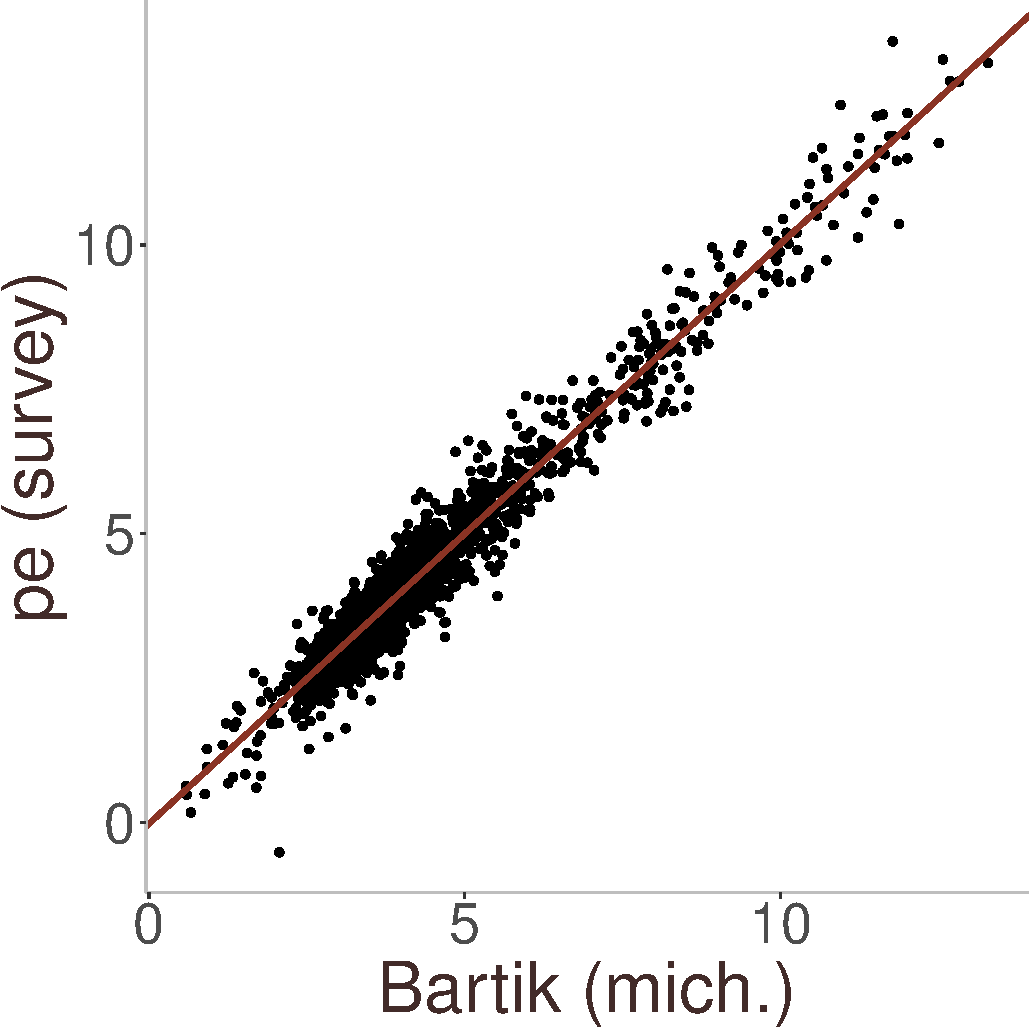
\includegraphics[width = 3in, height =3in]{figs/firststage}
%\input{figs/tex/firststage}
\caption{First stage: shares calculated from Michigan survey.  }\label{subfig:redform:stage1:michigan}
\end{subfigure}
\quad
\begin{subfigure}[t]{0.475\textwidth}
\centering
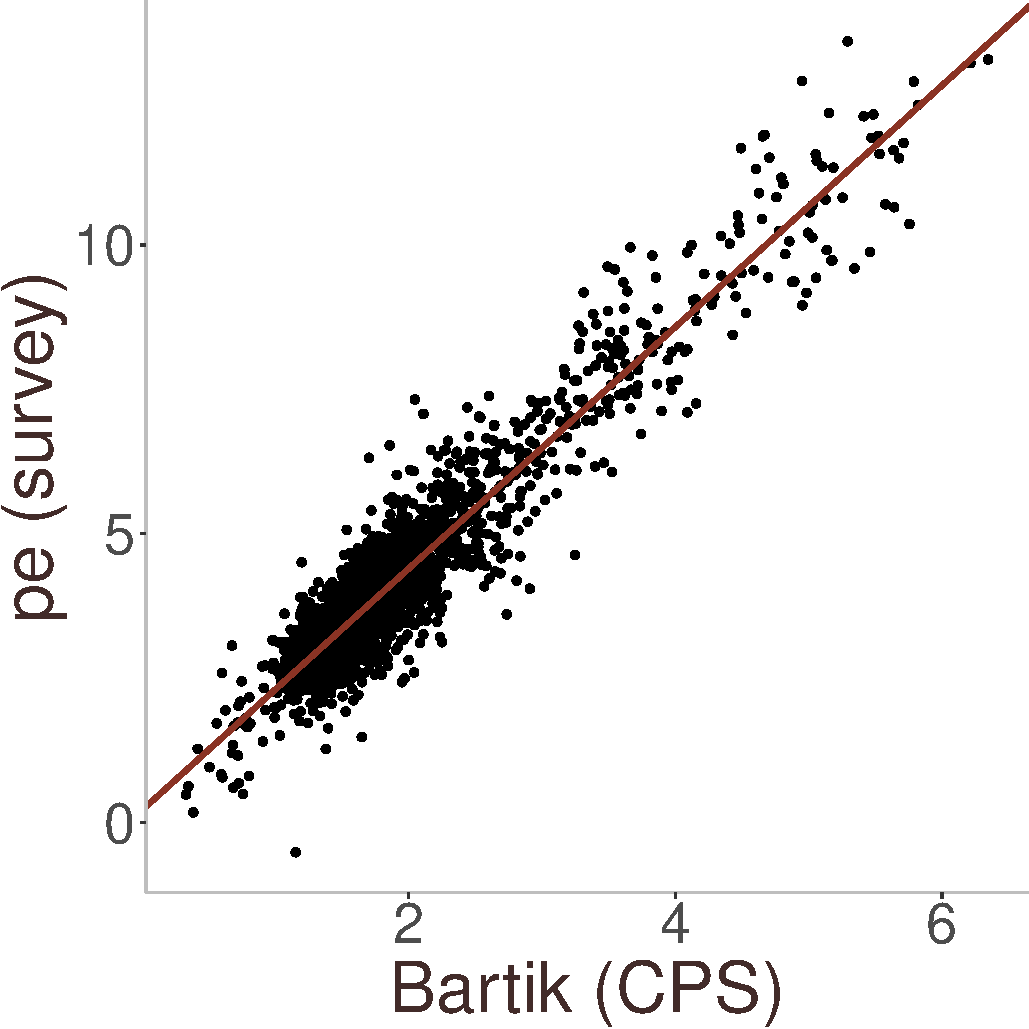
\includegraphics[width =3in, height =3in]{figs/firststage_cps}
%\input{figs/tex/firststage_cps}
\caption{First stage: shares calculated from 1978.1 CPS.}\label{subfig:redform:stage1:cps}
\end{subfigure}
\vfill
\begin{subfigure}[t]{0.475\textwidth}
\centering
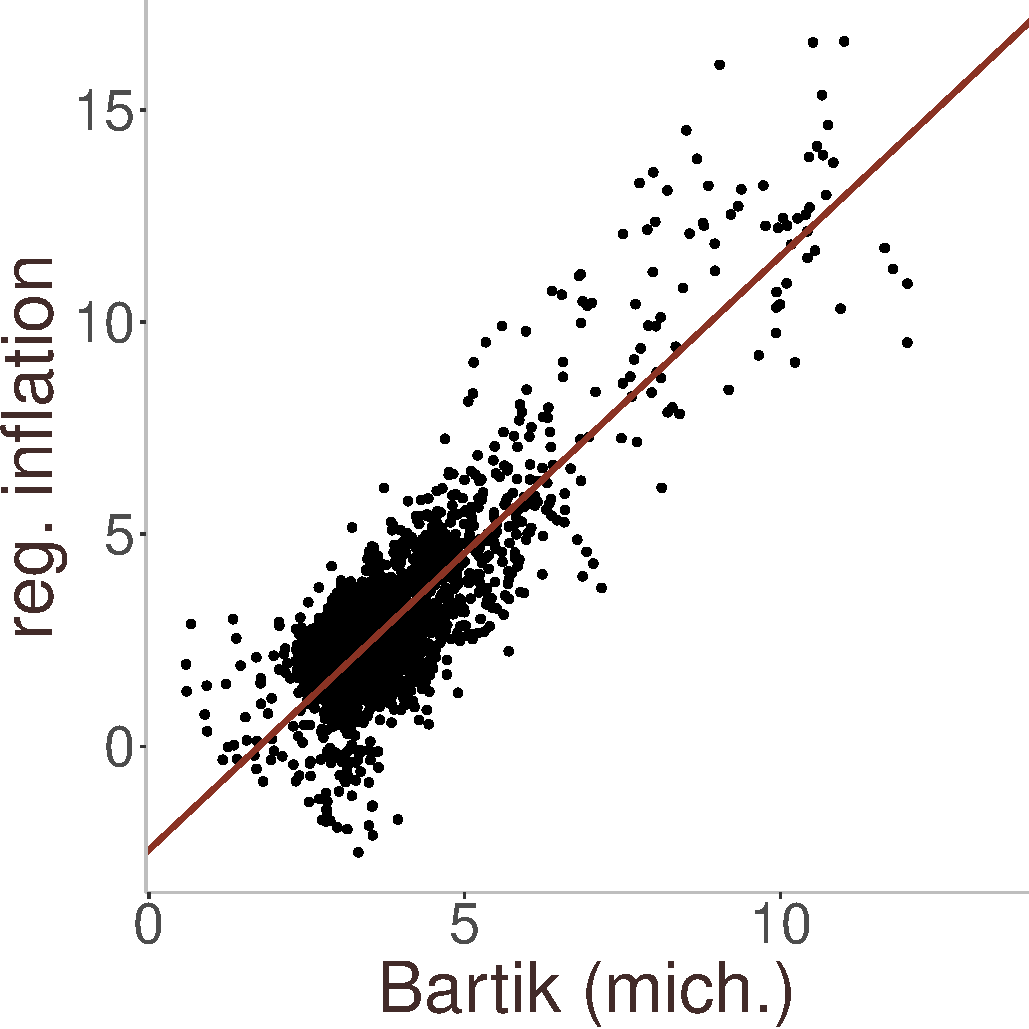
\includegraphics[width =3in, height =3in]{figs/redform}
%\input{figs/tex/redform}
\caption{OLS regression: Michigan shares.}\label{subfig:redform:stage2:michigan}
\end{subfigure}
\begin{subfigure}[t]{0.475\textwidth}
\centering
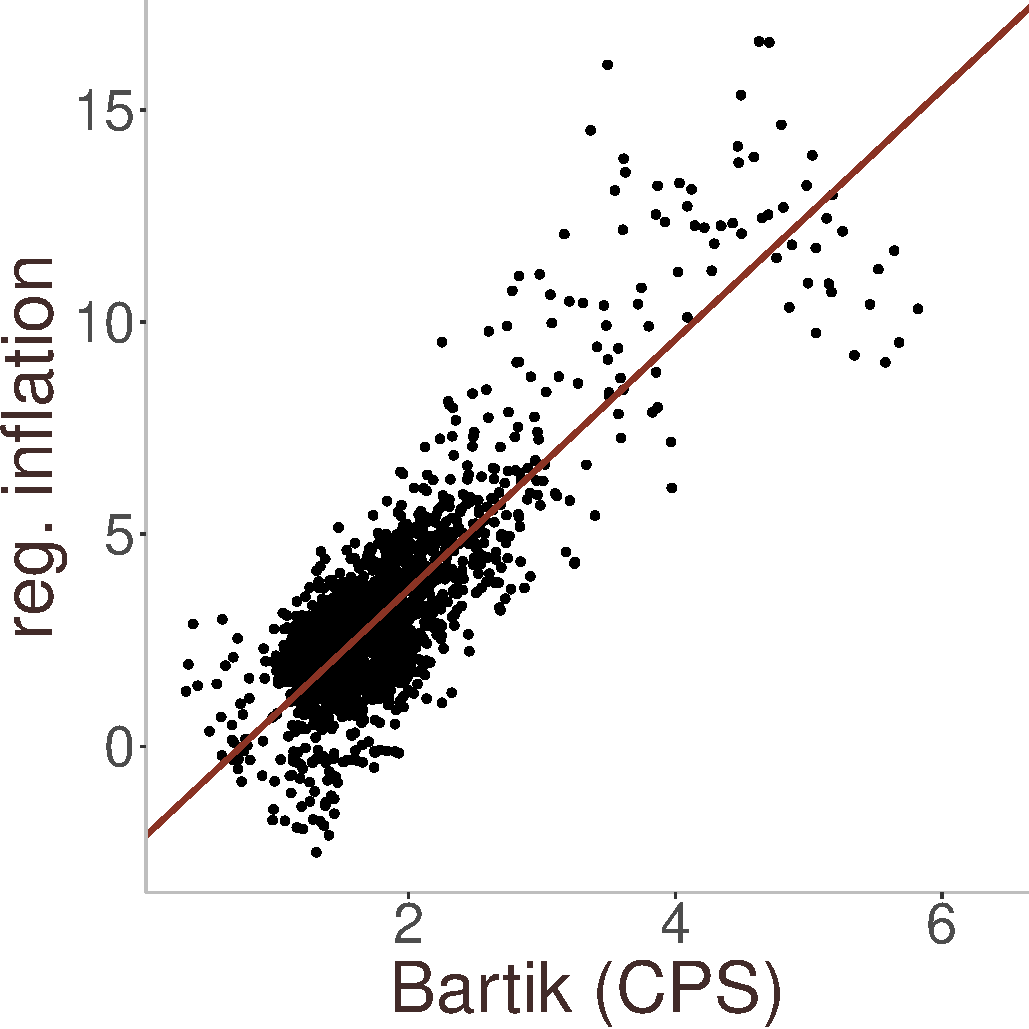
\includegraphics[width =3in, height =3in]{figs/redform_cps}
%\input{figs/tex/redform_cps}
\caption{OLS regression: CPS78 shares.}\label{subfig:redform:stage2:cps}
\end{subfigure}
\end{figure}


\subsection{2sls estimates}\label{mainEstimates}



Tables \ref{tab:base:out:2sls:stage1}-\ref{tab:base:out:2sls:stage2} present the two-stage least squares estimates of the impact that consumer inflation expectations have on regional inflation rates. Panel A details the coefficient estimate with the CPS 1978.1 population shares.  Panel B encompasses the Michigan survey measure of group shares. In both instances, constructing the instrument uses a regional leave-one-out approach. The results presented include a set of control variables and region and time-fixed effects—the latter controls for aggregate business cycle factors common to all regions. The control variables include the regional unemployment rate, four lags of inflation, survey measures for current and anticipated financial well-being and conditions, and regional expected gas prices.  Regional unemployment is instrumented by 12-month lags, though, the estimated pass-through is not sensitive to instrumenting.  Each numbered column corresponds to a model with or without fixed effects.  The model specification for each column is detailed in Table \ref{tab:base:out:2sls:stage2}.

\begin{table}

\caption{\label{tab:base:out:2sls:stage1}2SLS: first stage}
\centering
\begin{threeparttable}
\begin{tabular}[t]{lll}
\toprule
  & survey & CPS78\\
\midrule
\cellcolor{gray!6}{Dependent Var.:} & \cellcolor{gray!6}{pe} & \cellcolor{gray!6}{pe}\\
\addlinespace
 &  & \\
\addlinespace
\cellcolor{gray!6}{Bartik} & \cellcolor{gray!6}{0.2474*** (0.0611)} & \cellcolor{gray!6}{0.4478** (0.1448)}\\
\addlinespace
Controls & Yes & Yes\\
\addlinespace
\cellcolor{gray!6}{Fixed-Effects:} & \cellcolor{gray!6}{------------------} & \cellcolor{gray!6}{-----------------}\\
\addlinespace
REGION & Yes & Yes\\
\addlinespace
\cellcolor{gray!6}{TIME} & \cellcolor{gray!6}{Yes} & \cellcolor{gray!6}{Yes}\\
\addlinespace
\_\_\_\_\_\_\_\_\_\_\_\_\_\_\_ & \_\_\_\_\_\_\_\_\_\_\_\_\_\_\_\_\_\_ & \_\_\_\_\_\_\_\_\_\_\_\_\_\_\_\_\_\\
\addlinespace
\cellcolor{gray!6}{S.E. type} & \cellcolor{gray!6}{Drisco.-Kra. (L=4)} & \cellcolor{gray!6}{Drisc.-Kra. (L=4)}\\
\addlinespace
Observations & 1,387 & 1,387\\
\addlinespace
\cellcolor{gray!6}{R2} & \cellcolor{gray!6}{0.80353} & \cellcolor{gray!6}{0.80133}\\
\addlinespace
Within R2 & 0.13739 & 0.12774\\
\bottomrule
\end{tabular}
\begin{tablenotes}
\item \textit{Note: } 
\item First stage from 2sls panel regression of regional inflation on expected inflation. In the first stage, the Bartik instrument is a good predictor of inflation expectations. Instruments computed using a leave-one-out procedure. Survey is the shift-share instrument using Michigan survey shares. CPS78 is constructed from the 1978.1 CPS.
\item[1] Signif. codes: * = .05; ** = .01; *** = .001.
\end{tablenotes}
\end{threeparttable}
\end{table}

\begin{table}

\caption{\label{tab:base:out:2sls:stage2}2SLS: coefficient estimates}
\centering
\begin{threeparttable}
\begin{tabular}[t]{lll}
\toprule
  & survey & CPS78\\
\midrule
\cellcolor{gray!6}{Dependent Var.:} & \cellcolor{gray!6}{RegInf} & \cellcolor{gray!6}{RegInf}\\
\addlinespace
 &  & \\
\addlinespace
\cellcolor{gray!6}{pe} & \cellcolor{gray!6}{0.3351* (0.1406)} & \cellcolor{gray!6}{0.5465** (0.1939)}\\
\addlinespace
Controls & Yes & Yes\\
\addlinespace
\cellcolor{gray!6}{Fixed-Effects:} & \cellcolor{gray!6}{----------------} & \cellcolor{gray!6}{-----------------}\\
\addlinespace
REGION & Yes & Yes\\
\addlinespace
\cellcolor{gray!6}{TIME} & \cellcolor{gray!6}{Yes} & \cellcolor{gray!6}{Yes}\\
\addlinespace
\_\_\_\_\_\_\_\_\_\_\_\_\_\_\_ & \_\_\_\_\_\_\_\_\_\_\_\_\_\_\_\_ & \_\_\_\_\_\_\_\_\_\_\_\_\_\_\_\_\_\\
\addlinespace
\cellcolor{gray!6}{S.E. type} & \cellcolor{gray!6}{Dris.-Kra. (L=4)} & \cellcolor{gray!6}{Drisc.-Kra. (L=4)}\\
\addlinespace
Observations & 1,387 & 1,387\\
\addlinespace
\cellcolor{gray!6}{R2} & \cellcolor{gray!6}{0.95399} & \cellcolor{gray!6}{0.93969}\\
\addlinespace
Within R2 & 0.55429 & 0.41579\\
\bottomrule
\end{tabular}
\begin{tablenotes}
\item \textit{Note: } 
\item Coefficient estimates from 2sls panel regression of regional inflation on expected inflation. Instruments computed using a leave-one-out procedure. Survey is the shift-share instrument using Michigan survey shares. CPS78 is constructed from the 1978.1 CPS.
\item[1] Signif. codes: * = .05; ** = .01; *** = .001.
\end{tablenotes}
\end{threeparttable}
\end{table}


Table \ref{tab:base:out:2sls:stage1} provides first stage estimates. For each model, there are two columns for each of the two endogenous regressors. The Bartik instrument is relevant and has significant predictive power for inflation expectations. The Durbin-Wu-Hausman test statistic for endogeneity is 8.074, rejecting the consistency of OLS at a 1\% significance level. The first-stage F-statistic is 18.2 ($p^e$) and 296.3 ($U_R$), which is significant at the .1\% level. While the identifying variation in the shares is plausibly exogenous to regional inflation rates, in the case of CPS78, it is possible to probe the exogeneity assumption by examining whether those 1978 population shares are predictive of the regression covariates. In each case, there is no significant correlation between the covariates and the CPS group shares, and the regression coefficients are economically close to zero.

The second stage estimates in Table \ref{tab:base:out:2sls:stage2} identify a significant and positive effect from subjective inflation expectations to inflation rates. Using the Michigan survey shares, the estimated coefficient is $0.339$, so a 1\% increase in the average expected inflation rate in a region would lead to a 34 basis point increase in that region's inflation rate. The estimated coefficient is significant at the 1\% level. The estimated effect is stronger using the CPS 1978.1 population shares. The estimated coefficient is $0.560$, at a 1\% significance level. Here, the pass-through from inflation expectations to inflation is greater than $\nicefrac{1}{2}$.  

When comparing the 2sls coefficient estimates to those in Figure \ref{subfig:intro:reg}, OLS estimates, where the correlation between inflation expectations and inflation was around $0.06$, are biased downwards. The empirical model does not account for spatial spillovers. Much like the literature on regional fiscal multipliers, after accounting for cross-regional spillovers -- an increase in inflation expectations in one region also impacts the demand for goods produced in a different region -- the aggregate impact of expectations is stronger than the regional effect. In Figure \ref{subfig:intro:us} it was seen that the correlation between aggregate inflation expectations and aggregate inflation rates is $0.18$. A similar magnitude in the 2sls estimates would imply a pass-through of approximately $1.0-1.6$.  

The coefficient estimates are in line with the theoretical analysis in \cite{Werning:expectsWP}, which studies pass-through in a variety of conventional pricing models with time-dependent price rigidities while not making \emph{a priori} assumptions about the formation of subjective inflation expectations. While the pass-through from expectations to inflation can take any positive value, \cite{Werning:expectsWP} shows that for the Calvo and Taylor models of price stickiness, that pass-through should be in the range $\left[\nicefrac{1}{2},1\right]$, and possibly above one in a more general framework. While the regional estimates in Table \ref{tab:base:out:2sls:stage2} are on the lower end, or slightly below, of this range, after accounting for regional spillovers, the estimates are in line with the theoretical predictions.

The panel data is susceptible to a potential finite sample bias. Of particular concern are the data's ``small N/big T'' dimensions. Table \ref{tab:bias:out:2sls:stage2} applies a split-sample jackknife bias correction (\cite{FernandezValWeidner:FE}). After correcting for finite sample bias in both the cross-section and time dimensions, the estimated effect of inflation expectations increases slightly. Table \ref{tab:bias:out:2sls:stage2} provides the preferred estimate: a 1\% increase in inflation expectations leads to a 60 basis point increase in (regional) inflation.

\begin{table}
\centering
\caption{\label{tab:bias:out:2sls:stage2}Bias Correction}
\centering
\begin{threeparttable}
\begin{tabular}[t]{lrr}
\toprule
  & survey shares & CPS78 shares\\
\midrule
\cellcolor{gray!10}{coeff.} & \cellcolor{gray!10}{0.3753} & \cellcolor{gray!10}{0.5999}\\
se & 0.1356 & 0.1940\\
\bottomrule
\end{tabular}
\begin{tablenotes}
\item \textit{Note: } 
\item Applies the split-sample jacknife bias correction to the 2sls coefficient estimates. The column ``survey shares'' computes shares from Michigan survey,``CPS78 shares'' uses the CPS 1978.1 shares.
\end{tablenotes}
\end{threeparttable}
\end{table}


Another way to measure the impact of expectations is by estimating an impulse response function. The empirical model is not a vector autoregression, but a local projections approach can estimate the impulse response function.\footnote{See \cite{Jorda:LP}.}. The impulse response function comes from running 2sls regressions of the form
$$ E_t\pi^R_{t+h} = \delta_{R,h} + \beta_h\pi^e_{R,t} + \gamma'_h x_{R,h} + \mu_{t,h} + \varepsilon_{R,h,t}$$
for horizons $h=1,...,H$. The impulse response function then is given by $\left(\beta_h\right)_{1\leq h\leq H}$. The estimates are provided in Figure \ref{fig:base:irf}.

On impact, inflation expectations have a significant positive effect on inflation. There is a cyclical dampening process that is mean-reverting within 12 months. However, the confidence bands are wide in future quarters and cannot rule out any lingering impacts. Thus, the estimates suggest a moderate contemporaneous response to inflation from a shock to inflation expectations. The lack of a strongly persistent expectation effect could reflect the specific U.S. inflation history. It would be interesting to extend the analysis to countries with persistent or volatile inflation.


\begin{figure}
\centering
\caption{Impulse responses}\label{fig:base:irf}
\begin{subfigure}[t]{0.475\textwidth}
\centering
% Created by tikzDevice version 0.12.3.1 on 2023-11-03 11:03:16
% !TEX encoding = UTF-8 Unicode
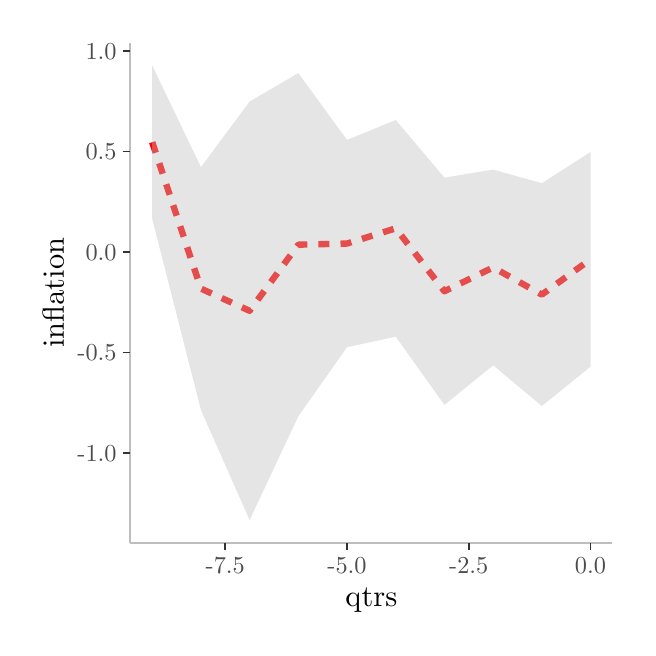
\begin{tikzpicture}[x=1pt,y=1pt]
\definecolor{fillColor}{RGB}{255,255,255}
\path[use as bounding box,fill=fillColor,fill opacity=0.00] (0,0) rectangle (216.81,216.81);
\begin{scope}
\path[clip] (  0.00,  0.00) rectangle (216.81,216.81);
\definecolor{drawColor}{RGB}{255,255,255}
\definecolor{fillColor}{RGB}{255,255,255}

\path[draw=drawColor,line width= 0.6pt,line join=round,line cap=round,fill=fillColor] (  0.00,  0.00) rectangle (216.81,216.81);
\end{scope}
\begin{scope}
\path[clip] ( 37.09, 30.69) rectangle (211.31,211.31);
\definecolor{drawColor}{RGB}{255,255,255}

\path[draw=drawColor,line width= 0.6pt,line join=round] ( 37.09, 63.17) --
	(211.31, 63.17);

\path[draw=drawColor,line width= 0.6pt,line join=round] ( 37.09, 99.46) --
	(211.31, 99.46);

\path[draw=drawColor,line width= 0.6pt,line join=round] ( 37.09,135.75) --
	(211.31,135.75);

\path[draw=drawColor,line width= 0.6pt,line join=round] ( 37.09,172.05) --
	(211.31,172.05);

\path[draw=drawColor,line width= 0.6pt,line join=round] ( 37.09,208.34) --
	(211.31,208.34);

\path[draw=drawColor,line width= 0.6pt,line join=round] ( 71.41, 30.69) --
	( 71.41,211.31);

\path[draw=drawColor,line width= 0.6pt,line join=round] (115.40, 30.69) --
	(115.40,211.31);

\path[draw=drawColor,line width= 0.6pt,line join=round] (159.40, 30.69) --
	(159.40,211.31);

\path[draw=drawColor,line width= 0.6pt,line join=round] (203.39, 30.69) --
	(203.39,211.31);
\definecolor{drawColor}{RGB}{255,0,0}

\path[draw=drawColor,line width= 2.3pt,dash pattern=on 4pt off 4pt ,line join=round] ( 45.01,175.42) --
	( 62.61,122.52) --
	( 80.20,114.50) --
	( 97.80,138.39) --
	(115.40,138.80) --
	(133.00,144.30) --
	(150.60,121.56) --
	(168.19,130.17) --
	(185.79,120.35) --
	(203.39,133.10);
\definecolor{fillColor}{RGB}{190,190,190}

\path[fill=fillColor,fill opacity=0.40] ( 45.01,203.10) --
	( 62.61,166.39) --
	( 80.20,190.11) --
	( 97.80,200.37) --
	(115.40,176.23) --
	(133.00,183.45) --
	(150.60,162.60) --
	(168.19,165.52) --
	(185.79,160.60) --
	(203.39,171.87) --
	(203.39, 94.33) --
	(185.79, 80.10) --
	(168.19, 94.83) --
	(150.60, 80.51) --
	(133.00,105.15) --
	(115.40,101.36) --
	( 97.80, 76.41) --
	( 80.20, 38.90) --
	( 62.61, 78.65) --
	( 45.01,147.74) --
	cycle;

\path[] ( 45.01,203.10) --
	( 62.61,166.39) --
	( 80.20,190.11) --
	( 97.80,200.37) --
	(115.40,176.23) --
	(133.00,183.45) --
	(150.60,162.60) --
	(168.19,165.52) --
	(185.79,160.60) --
	(203.39,171.87);

\path[] (203.39, 94.33) --
	(185.79, 80.10) --
	(168.19, 94.83) --
	(150.60, 80.51) --
	(133.00,105.15) --
	(115.40,101.36) --
	( 97.80, 76.41) --
	( 80.20, 38.90) --
	( 62.61, 78.65) --
	( 45.01,147.74);
\end{scope}
\begin{scope}
\path[clip] (  0.00,  0.00) rectangle (216.81,216.81);
\definecolor{drawColor}{RGB}{190,190,190}

\path[draw=drawColor,line width= 0.6pt,line join=round] ( 37.09, 30.69) --
	( 37.09,211.31);
\end{scope}
\begin{scope}
\path[clip] (  0.00,  0.00) rectangle (216.81,216.81);
\definecolor{drawColor}{gray}{0.30}

\node[text=drawColor,anchor=base east,inner sep=0pt, outer sep=0pt, scale=  0.88] at ( 32.14, 60.13) {-1.0};

\node[text=drawColor,anchor=base east,inner sep=0pt, outer sep=0pt, scale=  0.88] at ( 32.14, 96.43) {-0.5};

\node[text=drawColor,anchor=base east,inner sep=0pt, outer sep=0pt, scale=  0.88] at ( 32.14,132.72) {0.0};

\node[text=drawColor,anchor=base east,inner sep=0pt, outer sep=0pt, scale=  0.88] at ( 32.14,169.02) {0.5};

\node[text=drawColor,anchor=base east,inner sep=0pt, outer sep=0pt, scale=  0.88] at ( 32.14,205.31) {1.0};
\end{scope}
\begin{scope}
\path[clip] (  0.00,  0.00) rectangle (216.81,216.81);
\definecolor{drawColor}{gray}{0.20}

\path[draw=drawColor,line width= 0.6pt,line join=round] ( 34.34, 63.17) --
	( 37.09, 63.17);

\path[draw=drawColor,line width= 0.6pt,line join=round] ( 34.34, 99.46) --
	( 37.09, 99.46);

\path[draw=drawColor,line width= 0.6pt,line join=round] ( 34.34,135.75) --
	( 37.09,135.75);

\path[draw=drawColor,line width= 0.6pt,line join=round] ( 34.34,172.05) --
	( 37.09,172.05);

\path[draw=drawColor,line width= 0.6pt,line join=round] ( 34.34,208.34) --
	( 37.09,208.34);
\end{scope}
\begin{scope}
\path[clip] (  0.00,  0.00) rectangle (216.81,216.81);
\definecolor{drawColor}{RGB}{190,190,190}

\path[draw=drawColor,line width= 0.6pt,line join=round] ( 37.09, 30.69) --
	(211.31, 30.69);
\end{scope}
\begin{scope}
\path[clip] (  0.00,  0.00) rectangle (216.81,216.81);
\definecolor{drawColor}{gray}{0.20}

\path[draw=drawColor,line width= 0.6pt,line join=round] ( 71.41, 27.94) --
	( 71.41, 30.69);

\path[draw=drawColor,line width= 0.6pt,line join=round] (115.40, 27.94) --
	(115.40, 30.69);

\path[draw=drawColor,line width= 0.6pt,line join=round] (159.40, 27.94) --
	(159.40, 30.69);

\path[draw=drawColor,line width= 0.6pt,line join=round] (203.39, 27.94) --
	(203.39, 30.69);
\end{scope}
\begin{scope}
\path[clip] (  0.00,  0.00) rectangle (216.81,216.81);
\definecolor{drawColor}{gray}{0.30}

\node[text=drawColor,anchor=base,inner sep=0pt, outer sep=0pt, scale=  0.88] at ( 71.41, 19.68) {-7.5};

\node[text=drawColor,anchor=base,inner sep=0pt, outer sep=0pt, scale=  0.88] at (115.40, 19.68) {-5.0};

\node[text=drawColor,anchor=base,inner sep=0pt, outer sep=0pt, scale=  0.88] at (159.40, 19.68) {-2.5};

\node[text=drawColor,anchor=base,inner sep=0pt, outer sep=0pt, scale=  0.88] at (203.39, 19.68) {0.0};
\end{scope}
\begin{scope}
\path[clip] (  0.00,  0.00) rectangle (216.81,216.81);
\definecolor{drawColor}{RGB}{0,0,0}

\node[text=drawColor,anchor=base,inner sep=0pt, outer sep=0pt, scale=  1.10] at (124.20,  7.64) {qtrs};
\end{scope}
\begin{scope}
\path[clip] (  0.00,  0.00) rectangle (216.81,216.81);
\definecolor{drawColor}{RGB}{0,0,0}

\node[text=drawColor,rotate= 90.00,anchor=base,inner sep=0pt, outer sep=0pt, scale=  1.10] at ( 13.08,121.00) {inflation};
\end{scope}
\end{tikzpicture}

\caption{cps shares}
\end{subfigure}
\quad
\begin{subfigure}[t]{0.475\textwidth}
\centering
% Created by tikzDevice version 0.12.3.1 on 2023-10-19 11:54:22
% !TEX encoding = UTF-8 Unicode
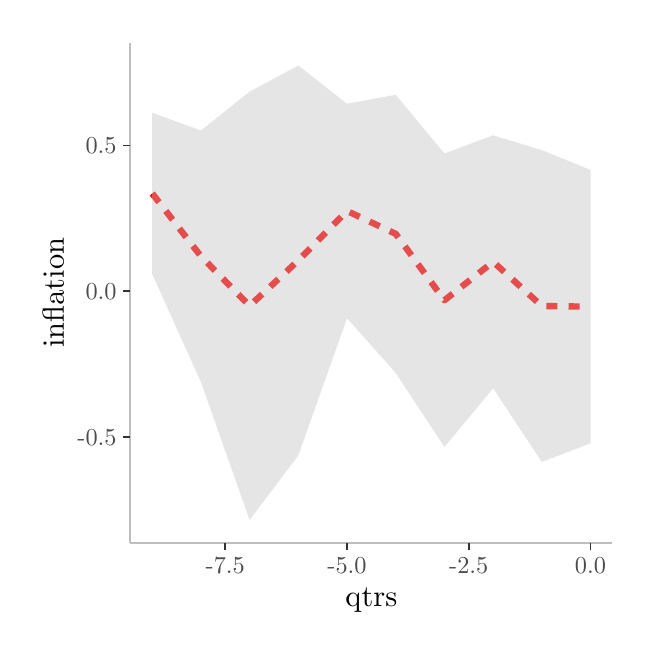
\begin{tikzpicture}[x=1pt,y=1pt]
\definecolor{fillColor}{RGB}{255,255,255}
\path[use as bounding box,fill=fillColor,fill opacity=0.00] (0,0) rectangle (216.81,216.81);
\begin{scope}
\path[clip] (  0.00,  0.00) rectangle (216.81,216.81);
\definecolor{drawColor}{RGB}{255,255,255}
\definecolor{fillColor}{RGB}{255,255,255}

\path[draw=drawColor,line width= 0.6pt,line join=round,line cap=round,fill=fillColor] (  0.00,  0.00) rectangle (216.81,216.81);
\end{scope}
\begin{scope}
\path[clip] ( 37.09, 30.69) rectangle (211.31,211.31);
\definecolor{drawColor}{RGB}{255,255,255}

\path[draw=drawColor,line width= 0.6pt,line join=round] ( 37.09, 68.88) --
	(211.31, 68.88);

\path[draw=drawColor,line width= 0.6pt,line join=round] ( 37.09,121.58) --
	(211.31,121.58);

\path[draw=drawColor,line width= 0.6pt,line join=round] ( 37.09,174.28) --
	(211.31,174.28);

\path[draw=drawColor,line width= 0.6pt,line join=round] ( 71.41, 30.69) --
	( 71.41,211.31);

\path[draw=drawColor,line width= 0.6pt,line join=round] (115.40, 30.69) --
	(115.40,211.31);

\path[draw=drawColor,line width= 0.6pt,line join=round] (159.40, 30.69) --
	(159.40,211.31);

\path[draw=drawColor,line width= 0.6pt,line join=round] (203.39, 30.69) --
	(203.39,211.31);
\definecolor{drawColor}{RGB}{255,0,0}

\path[draw=drawColor,line width= 2.3pt,dash pattern=on 4pt off 4pt ,line join=round] ( 45.01,156.90) --
	( 62.61,134.20) --
	( 80.20,116.30) --
	( 97.80,132.68) --
	(115.40,150.58) --
	(133.00,142.31) --
	(150.60,118.31) --
	(168.19,132.20) --
	(185.79,116.23) --
	(203.39,116.00);
\definecolor{fillColor}{RGB}{190,190,190}

\path[fill=fillColor,fill opacity=0.40] ( 45.01,186.05) --
	( 62.61,179.64) --
	( 80.20,193.70) --
	( 97.80,203.10) --
	(115.40,189.31) --
	(133.00,192.56) --
	(150.60,171.34) --
	(168.19,177.89) --
	(185.79,172.57) --
	(203.39,165.39) --
	(203.39, 66.62) --
	(185.79, 59.89) --
	(168.19, 86.51) --
	(150.60, 65.29) --
	(133.00, 92.06) --
	(115.40,111.84) --
	( 97.80, 62.27) --
	( 80.20, 38.90) --
	( 62.61, 88.76) --
	( 45.01,127.74) --
	cycle;

\path[] ( 45.01,186.05) --
	( 62.61,179.64) --
	( 80.20,193.70) --
	( 97.80,203.10) --
	(115.40,189.31) --
	(133.00,192.56) --
	(150.60,171.34) --
	(168.19,177.89) --
	(185.79,172.57) --
	(203.39,165.39);

\path[] (203.39, 66.62) --
	(185.79, 59.89) --
	(168.19, 86.51) --
	(150.60, 65.29) --
	(133.00, 92.06) --
	(115.40,111.84) --
	( 97.80, 62.27) --
	( 80.20, 38.90) --
	( 62.61, 88.76) --
	( 45.01,127.74);
\end{scope}
\begin{scope}
\path[clip] (  0.00,  0.00) rectangle (216.81,216.81);
\definecolor{drawColor}{RGB}{190,190,190}

\path[draw=drawColor,line width= 0.6pt,line join=round] ( 37.09, 30.69) --
	( 37.09,211.31);
\end{scope}
\begin{scope}
\path[clip] (  0.00,  0.00) rectangle (216.81,216.81);
\definecolor{drawColor}{gray}{0.30}

\node[text=drawColor,anchor=base east,inner sep=0pt, outer sep=0pt, scale=  0.88] at ( 32.14, 65.85) {-0.5};

\node[text=drawColor,anchor=base east,inner sep=0pt, outer sep=0pt, scale=  0.88] at ( 32.14,118.55) {0.0};

\node[text=drawColor,anchor=base east,inner sep=0pt, outer sep=0pt, scale=  0.88] at ( 32.14,171.25) {0.5};
\end{scope}
\begin{scope}
\path[clip] (  0.00,  0.00) rectangle (216.81,216.81);
\definecolor{drawColor}{gray}{0.20}

\path[draw=drawColor,line width= 0.6pt,line join=round] ( 34.34, 68.88) --
	( 37.09, 68.88);

\path[draw=drawColor,line width= 0.6pt,line join=round] ( 34.34,121.58) --
	( 37.09,121.58);

\path[draw=drawColor,line width= 0.6pt,line join=round] ( 34.34,174.28) --
	( 37.09,174.28);
\end{scope}
\begin{scope}
\path[clip] (  0.00,  0.00) rectangle (216.81,216.81);
\definecolor{drawColor}{RGB}{190,190,190}

\path[draw=drawColor,line width= 0.6pt,line join=round] ( 37.09, 30.69) --
	(211.31, 30.69);
\end{scope}
\begin{scope}
\path[clip] (  0.00,  0.00) rectangle (216.81,216.81);
\definecolor{drawColor}{gray}{0.20}

\path[draw=drawColor,line width= 0.6pt,line join=round] ( 71.41, 27.94) --
	( 71.41, 30.69);

\path[draw=drawColor,line width= 0.6pt,line join=round] (115.40, 27.94) --
	(115.40, 30.69);

\path[draw=drawColor,line width= 0.6pt,line join=round] (159.40, 27.94) --
	(159.40, 30.69);

\path[draw=drawColor,line width= 0.6pt,line join=round] (203.39, 27.94) --
	(203.39, 30.69);
\end{scope}
\begin{scope}
\path[clip] (  0.00,  0.00) rectangle (216.81,216.81);
\definecolor{drawColor}{gray}{0.30}

\node[text=drawColor,anchor=base,inner sep=0pt, outer sep=0pt, scale=  0.88] at ( 71.41, 19.68) {-7.5};

\node[text=drawColor,anchor=base,inner sep=0pt, outer sep=0pt, scale=  0.88] at (115.40, 19.68) {-5.0};

\node[text=drawColor,anchor=base,inner sep=0pt, outer sep=0pt, scale=  0.88] at (159.40, 19.68) {-2.5};

\node[text=drawColor,anchor=base,inner sep=0pt, outer sep=0pt, scale=  0.88] at (203.39, 19.68) {0.0};
\end{scope}
\begin{scope}
\path[clip] (  0.00,  0.00) rectangle (216.81,216.81);
\definecolor{drawColor}{RGB}{0,0,0}

\node[text=drawColor,anchor=base,inner sep=0pt, outer sep=0pt, scale=  1.10] at (124.20,  7.64) {qtrs};
\end{scope}
\begin{scope}
\path[clip] (  0.00,  0.00) rectangle (216.81,216.81);
\definecolor{drawColor}{RGB}{0,0,0}

\node[text=drawColor,rotate= 90.00,anchor=base,inner sep=0pt, outer sep=0pt, scale=  1.10] at ( 13.08,121.00) {inflation};
\end{scope}
\end{tikzpicture}

\caption{michigan shares}
\end{subfigure}
\end{figure}

\subsection{Identification and interpretation}

Equation (\ref{LOM}) suggests the presence of heterogeneous treatment effects from group-specific inflation expectations. The empirical procedure exploits the heterogeneity in group inflation expectations and plausibly exogenous variation in group shares to instrument for regional inflation expectations. While there are 160 different groups, their group shares can vary across regions and time, so economically, some groups may be more important than others. The interpretation of the identifying variation compares regional inflation and expectations in regions with differing degrees of exposure to these critical groups. This section explores these observations.

\cite{Pinkhametal:AER2020} exploits that the Bartik instrument estimate is a weighted average of many just identified instruments and calculate the estimation weights (``Rotemberg weights'') that drive identification. The analysis here applies the approach developed in \cite{Pinkhametal:AER2020}. The Rotemberg weights arise from the decomposition
$$ \beta = \sum_g \alpha_g\beta_g$$
where $\beta_g$ is the just identified estimate for group $g$. The weight $\alpha_g$ is the sensitivity of the overall estimate $\beta$ to bias emanating from misspecification in a group $g$. That is, the $\alpha_g$'s give us a measure of which groups are most driving identification and, formally, which groups to probe for endogeneity in the instrument.  

\begin{table}

\caption{\label{tab:rotweights:cps}Top-10 weighted groups: CPS shares}
\centering
\begin{threeparttable}
\begin{tabular}[t]{lrr}
\toprule
group & $\alpha_g$ & $\beta_g$\\
\midrule
\cellcolor{gray!6}{Ml,35-49,c,M,K} & \cellcolor{gray!6}{0.0151} & \cellcolor{gray!6}{1.3824}\\
\addlinespace
Ml,25-34,c,M,K & 0.0141 & 1.5614\\
\addlinespace
\cellcolor{gray!6}{Fl,35-49,c,M,K} & \cellcolor{gray!6}{0.0124} & \cellcolor{gray!6}{1.5935}\\
\addlinespace
F,25-34,c,S,NK & 0.0120 & 1.5397\\
\addlinespace
\cellcolor{gray!6}{Ml,25-34,hs,M,K} & \cellcolor{gray!6}{0.0120} & \cellcolor{gray!6}{1.5080}\\
\addlinespace
Fl,25-34,hs,M,K & 0.0117 & 1.3970\\
\addlinespace
\cellcolor{gray!6}{Ml,25-34,hs,M,NK} & \cellcolor{gray!6}{0.0110} & \cellcolor{gray!6}{1.5619}\\
\addlinespace
Fl,25-34,<hs,M,K & 0.0106 & 1.7735\\
\addlinespace
\cellcolor{gray!6}{Ml,25-34,c,S,NK} & \cellcolor{gray!6}{0.0101} & \cellcolor{gray!6}{1.4090}\\
\addlinespace
Ml,35-49,c,S,NK & 0.0101 & 1.4652\\
\bottomrule
\end{tabular}
\begin{tablenotes}
\item \textit{Note: } 
\item Group labels ordered: sex, age, educ., marital, children. Top-10 weighted groups according to the ``Rotemberg'' weights as in Bartik paper.
\end{tablenotes}
\end{threeparttable}
\end{table}

\begin{table}
\centering
\caption{\label{tab:rotweights:michigan}Top 10 weighted groups: Michigan shares}
\centering
\begin{threeparttable}
\begin{tabular}[t]{lrr}
\toprule
group id & $\alpha_g$ & $\beta_g$\\
\midrule
\cellcolor{gray!10}{Ml,18-24,h.s.,M,NK} & \cellcolor{gray!10}{0.0330} & \cellcolor{gray!10}{1.5574}\\
\addlinespace
Ml,25-34,h.s.,M,NK & 0.0177 & 1.7646\\
\addlinespace
\cellcolor{gray!10}{Ml,18-24,c+,M,NK} & \cellcolor{gray!10}{0.0174} & \cellcolor{gray!10}{1.5920}\\
\addlinespace
Fl,18-24,s.h.s.,M,NK & 0.0160 & 1.4804\\
\addlinespace
\cellcolor{gray!10}{Ml,18-24,s.c.,M,NK} & \cellcolor{gray!10}{0.0155} & \cellcolor{gray!10}{1.4664}\\
\addlinespace
Ml,18-24,h.s.,M,K & 0.0149 & 1.6477\\
\addlinespace
\cellcolor{gray!10}{Fl,18-24,h.s.,M,NK} & \cellcolor{gray!10}{0.0146} & \cellcolor{gray!10}{1.6288}\\
\addlinespace
Fl,18-24,s.c.,M,K & 0.0146 & 1.6878\\
\addlinespace
\cellcolor{gray!10}{Ml,35-49,s.c.,M,NK} & \cellcolor{gray!10}{0.0146} & \cellcolor{gray!10}{1.4254}\\
\addlinespace
Fl,25-34,h.s.,M,NK & 0.0141 & 1.8965\\
\bottomrule
\end{tabular}
\begin{tablenotes}
\item \textit{Note: } 
\item Group labels ordered: sex, age, educ., marital, children. Top-10 weighted groups according to the ``Rotemberg'' weights as in Goldsmith-Pinkham, et al (2020).
\end{tablenotes}
\end{threeparttable}
\end{table}


Tables \ref{tab:rotweights:cps}-\ref{tab:rotweights:michigan} detail the 10 groups with the highest Rotemberg weights, $\alpha_g$. Table \ref{tab:rotweights:cps} is for the case where the instrument is the CPS shares, and Table \ref{tab:rotweights:michigan} uses the Michigan survey shares. The table also lists the just-identified estimate for these top 10 groups. In both cases, the highest weighted groups are mostly younger with high school or above education. In the case of the CPS estimates, the highest weighted groups are 25-49 years old, and 6 of the groups have college degrees. Seven of the groups have been married with children. Using the Michigan shares instrument, Table \ref{tab:rotweights:michigan} shows that the top-10 groups are even younger than those identified by the CPS instrument. Most groups are 18-24, with one 25-34 and one 35-49. These groups also have at least a high school degree, though using the Michigan survey shares, 5/10 of the top groups have a high school degree, 3 have some college, and 1 have college degrees or more. Almost all of these groups are married without children.

If the estimates in Table \ref{tab:base:out:2sls:stage2} capture heterogeneous treatment effects across groups, then it is not surprising that the two different Bartik instruments estimate different treatment effects. The Michigan shares instrument can capture shifting demographic trends in the U.S., whereas the CPS share instrument exploited differential exposure to population shares in 1978. In both cases, the group-specific effect $\beta_g$ is positive and significantly above 1 for these heavily weighted groups.  

Table \ref{tab:rotweights:groups} looks at the group weights for broader demographic groups. Reported is the sum of the $\alpha_g$'s for broader groups classified by just one demographic characteristic, e.g., sex, age, or education. Regardless of the instrument, men are weighted slightly above women, and groups above 50 receive a small share of the weights. In the CPS share instrument, as seen in Table \ref{tab:rotweights:cps}, the 25-34 age group is most heavily weighted, followed by 35-49, then 18-24. In the Michigan survey, the Rotemberg weights are declining monotonically with age. The CPS share instrument weights those with a college degree more heavily, while the Michigan survey is roughly equally sensitive to those with a high school or college degree.

Figures \ref{fig:rotweights:group}-\ref{fig:rotweights:time} provide a graphical interpretation of these heterogeneous effects. Figure \ref{fig:rotweights:group} plots the $\beta_g$ against the corresponding first stage F-statistic $F_g$. The circles denote estimates with positive $\alpha_g$, and the triangles are the negative weights. The size of the points reflects the Rotemberg weight. So, the large circles correspond to the top-10 groups in Table \ref{tab:rotweights:michigan}. Finally, the dashed line is the estimated average treatment effect. Notice that there are few negatively weighted groups, so it is natural to interpret the estimate as capturing a heterogeneous treatment effect. Second, the most heavily weighted estimates reflect groups with significant pass-through but still lie relatively close to the average effect.  

Meanwhile, Figure \ref{fig:rotweights:time} plots the Rotemberg weight for each month in the sample. Rather than summing Rotemberg weights across groups, one can also calculate which particular periods provide most of the identifying variation. Given U.S. macroeconomic history, the estimation weights in Figure \ref{fig:rotweights:time} align with what we expect. The highest weighted periods are at the end of the 1970's Great Inflation and the subsequent Volcker disinflation. The other heavily weighted periods are the Great Recession (2007-2009) and the post-pandemic accelerating inflation. These weights are sensible and help give confidence in the overall empirical strategy.

From these findings, it is reasonable to conclude that the estimated impact of expectations on inflation reflects a weighted average of heterogeneous groups. Those groups that receive the most weight tend to be younger, married, and with at least a high school degree. The identifying variation is also driven strongly by volatile periods, suggesting non-linearities in mapping inflation expectations to outcomes. By seeking exogenous variation in inflation expectations, the approach here is silent on the self-referentiality of inflation, the impact of expectations on inflation, and then inflation on expectations. However, the time-varying estimation weights seem consistent with non-linear models of endogenously heterogeneous expectations as in \cite{BranchEJ2004}, \cite{BrockHommesEconometrica1997}.



%\begin{figure}
%\centering
%\caption{Estimation weights across groups: heterogeneous effects.}
%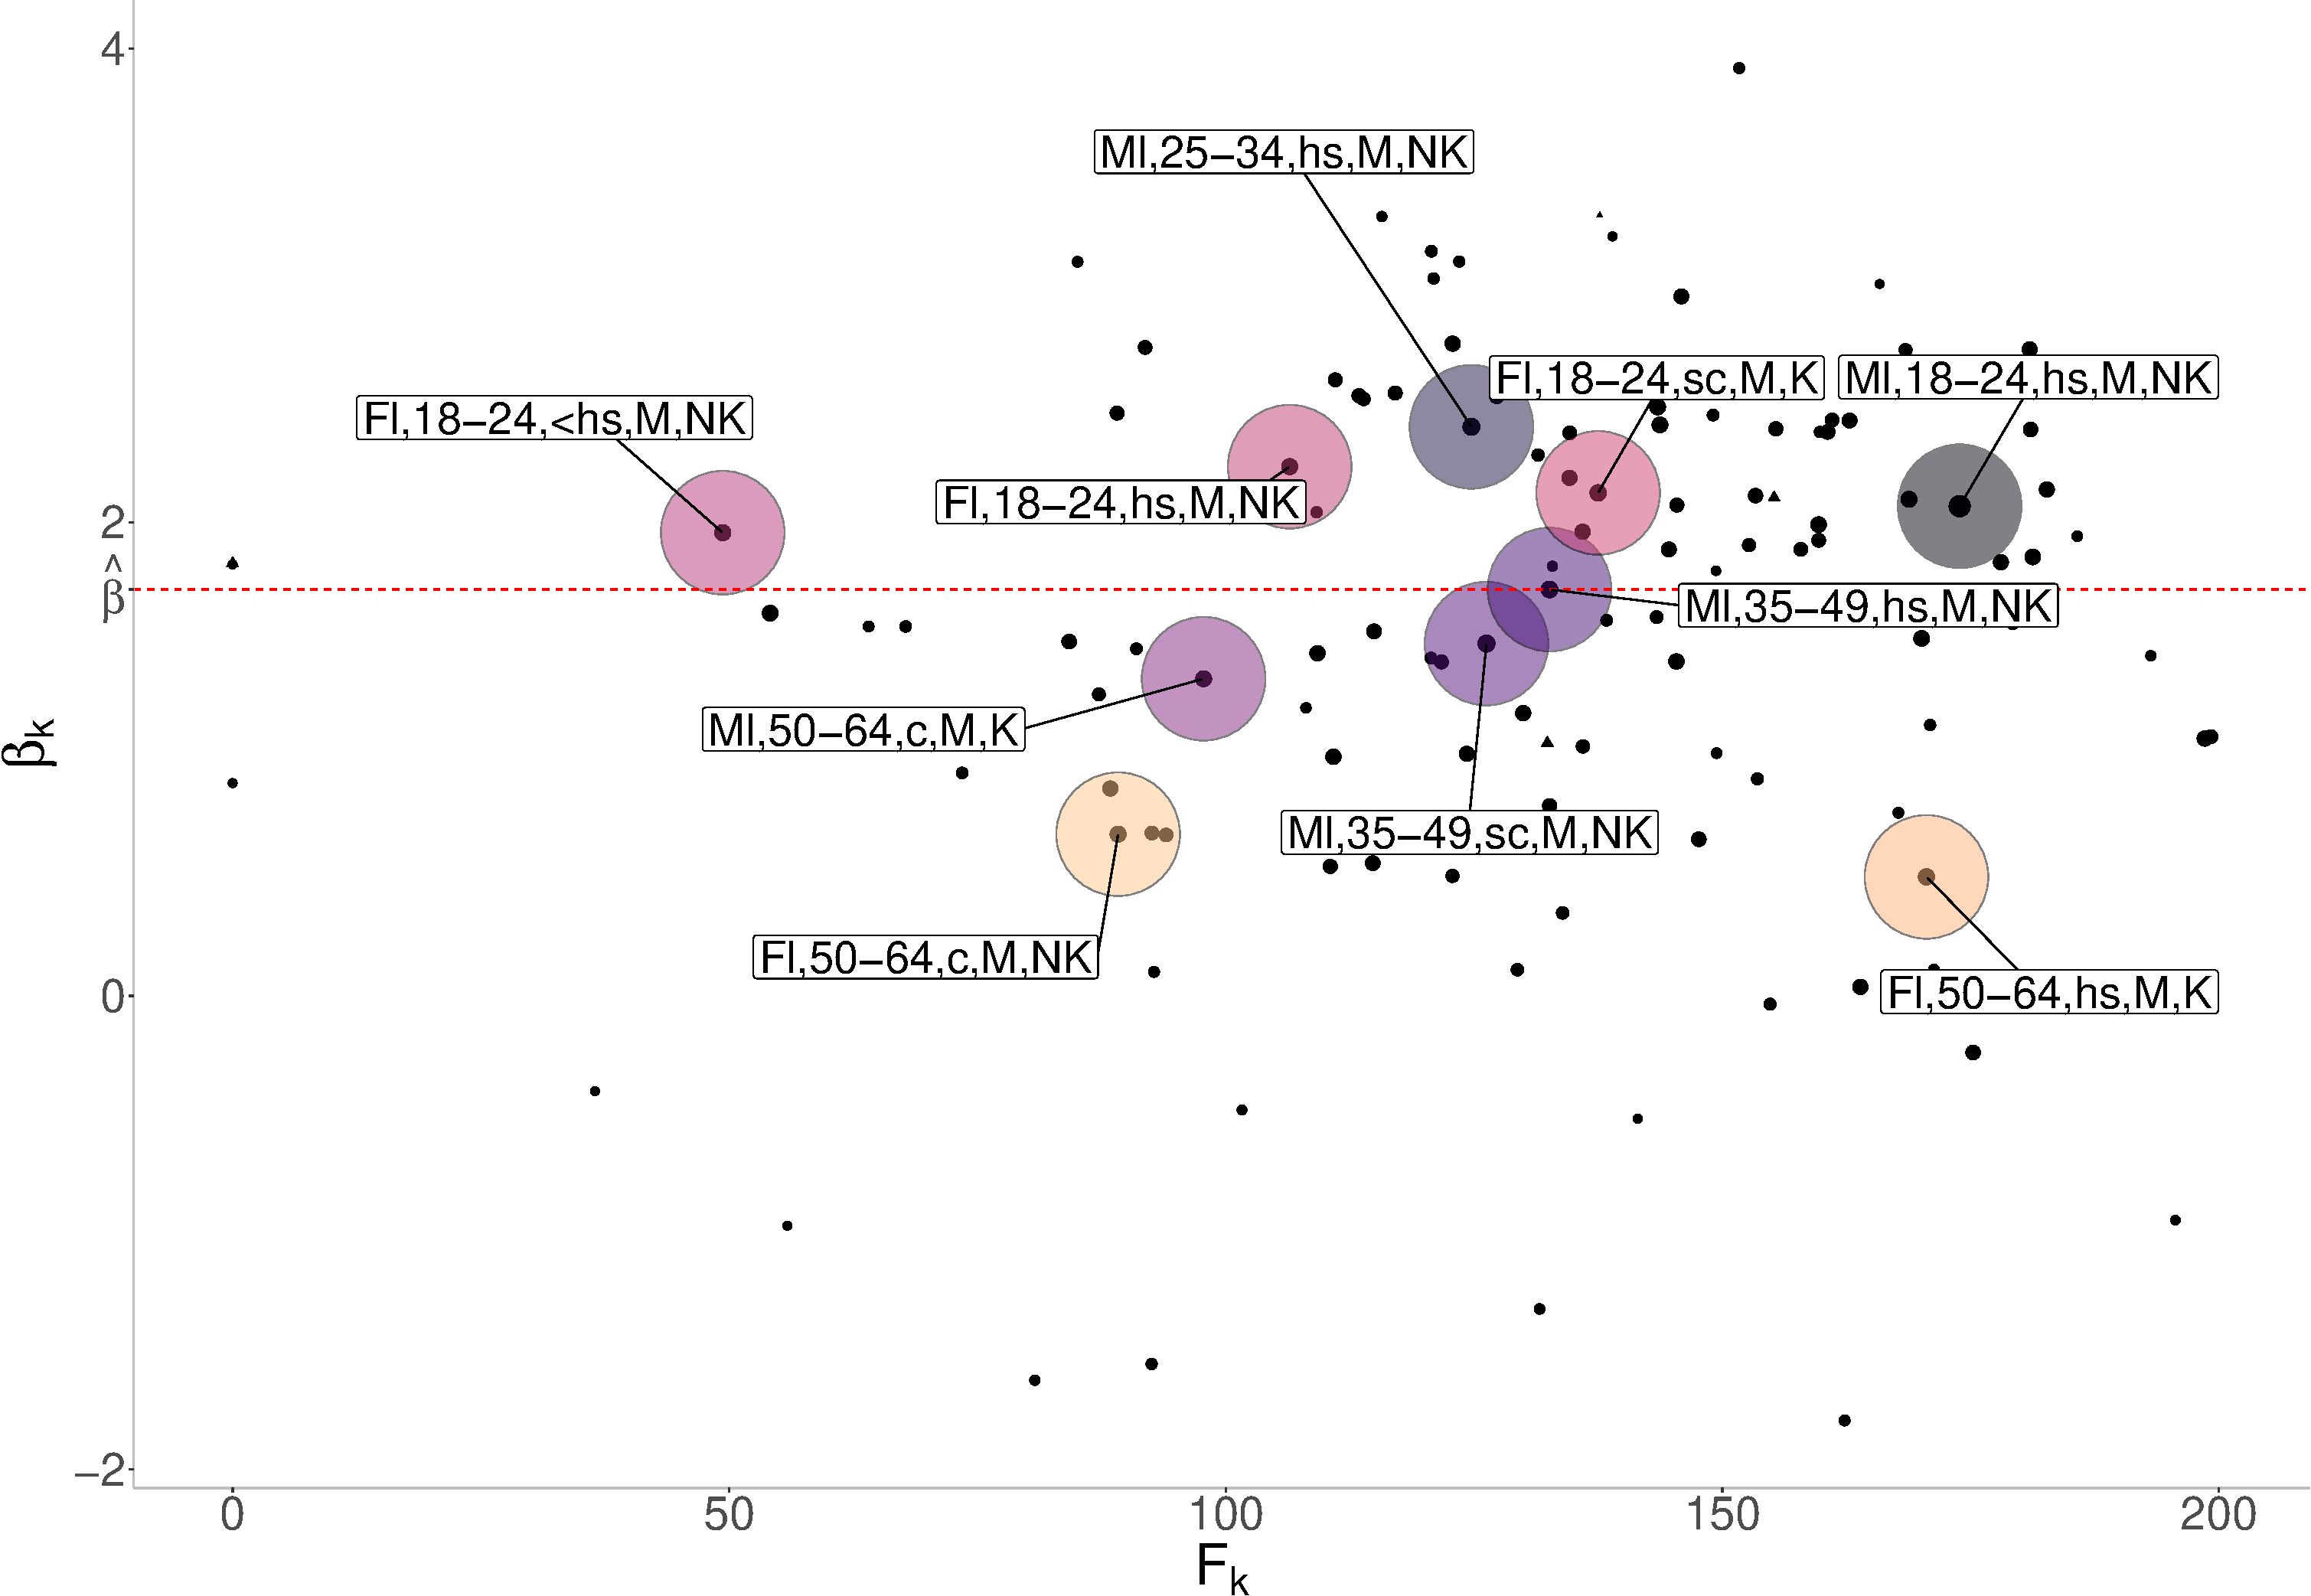
\includegraphics[height=.85\textwidth, width =\textwidth]{figs/weights.pdf}
%\end{figure}

\begin{figure}
\centering
\caption{Estimation weights across groups: Michigan shares. Scatter plot of each group's first stage F-statistic against its just-identified effect. The size of the circle represents the Rotemberg weight. The largest circle are the top-10 groups. Triangles denote negative weights.}\label{fig:rotweights:group}
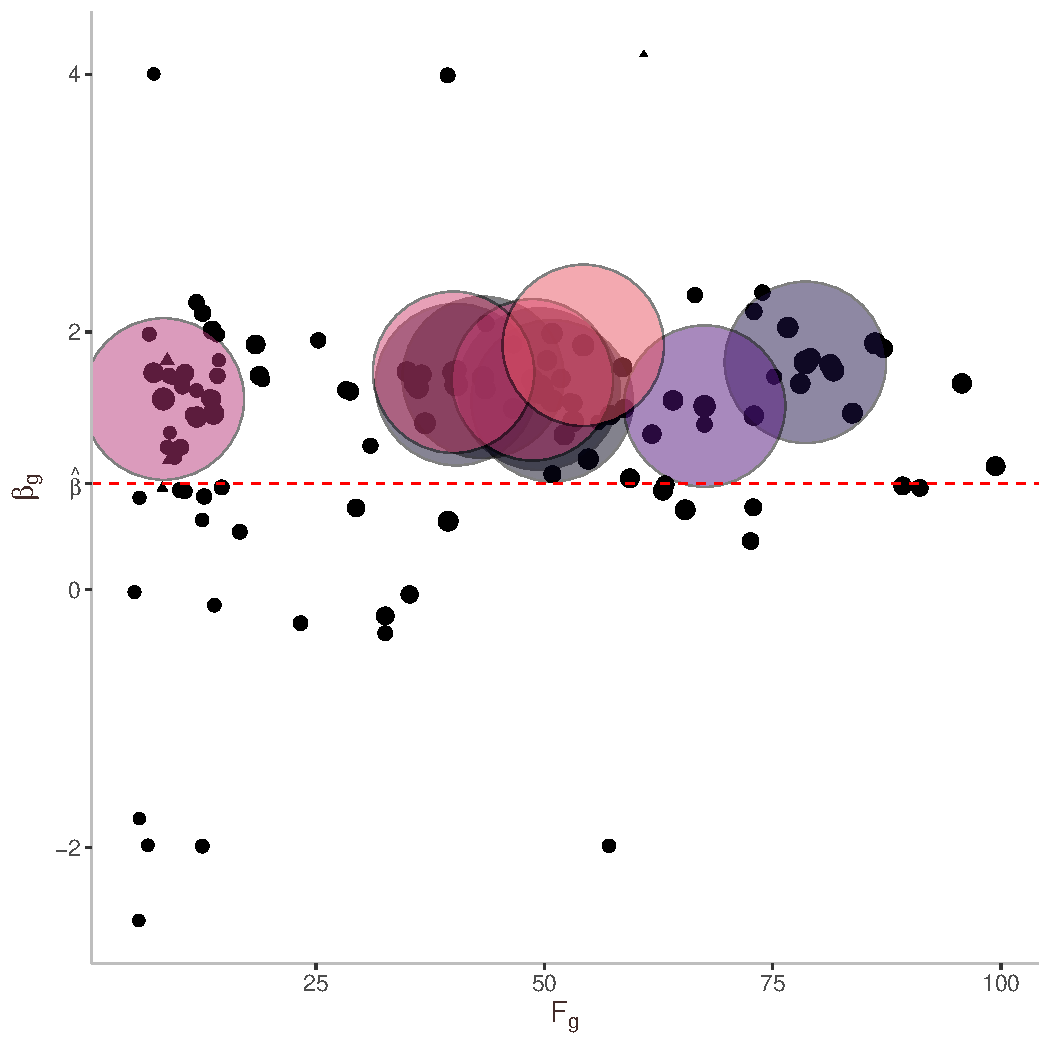
\includegraphics[height=.85\textwidth, width = .85\textwidth]{figs/weightsout}
\end{figure}

\begin{figure}
\centering
\caption{Estimation weights across time.}\label{fig:rotweights:time}
% Created by tikzDevice version 0.12.3.1 on 2023-10-23 16:07:10
% !TEX encoding = UTF-8 Unicode
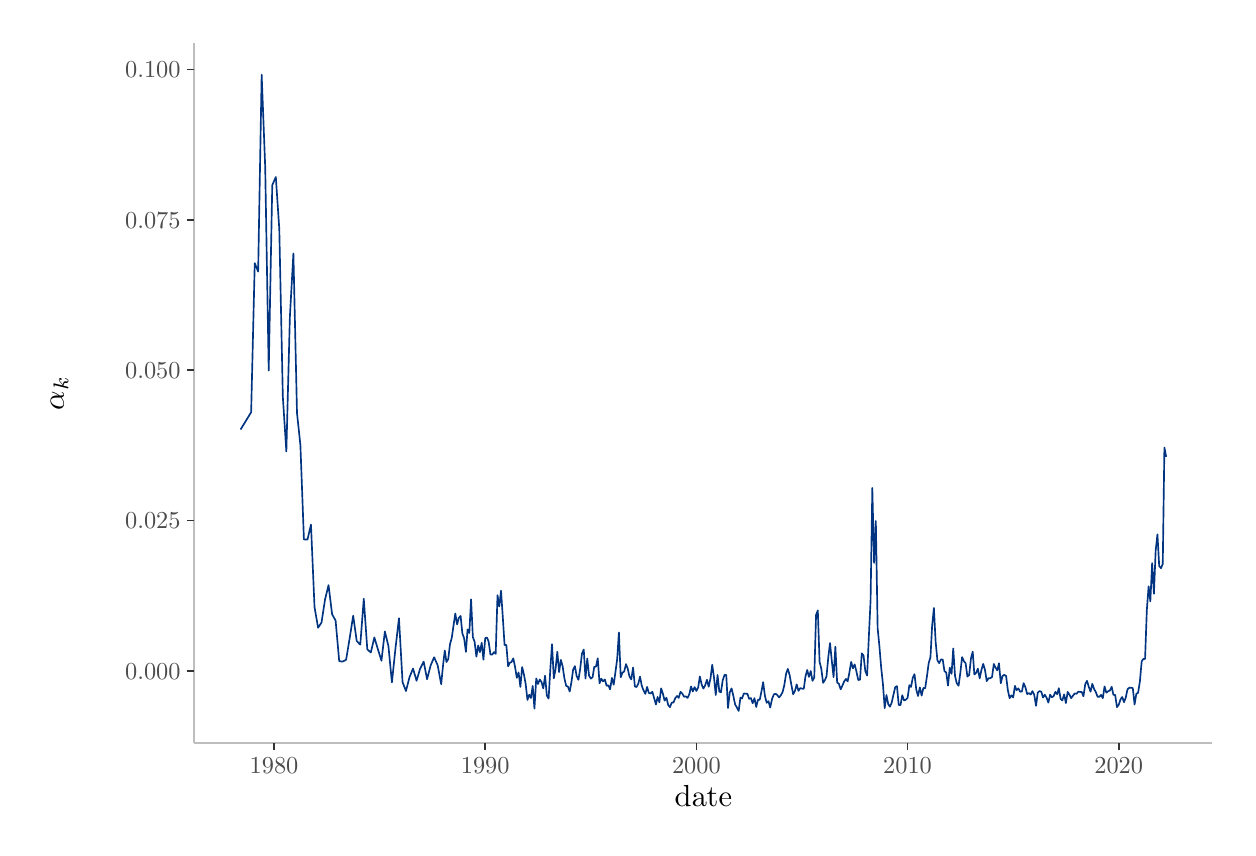
\begin{tikzpicture}[x=1pt,y=1pt]
\definecolor{fillColor}{RGB}{255,255,255}
\path[use as bounding box,fill=fillColor,fill opacity=0.00] (0,0) rectangle (433.62,289.08);
\begin{scope}
\path[clip] (  0.00,  0.00) rectangle (433.62,289.08);
\definecolor{drawColor}{RGB}{255,255,255}
\definecolor{fillColor}{RGB}{255,255,255}

\path[draw=drawColor,line width= 0.6pt,line join=round,line cap=round,fill=fillColor] (  0.00,  0.00) rectangle (433.62,289.08);
\end{scope}
\begin{scope}
\path[clip] ( 60.20, 30.69) rectangle (428.12,283.58);
\definecolor{drawColor}{RGB}{255,255,255}

\path[draw=drawColor,line width= 0.6pt,line join=round] ( 60.20, 56.71) --
	(428.12, 56.71);

\path[draw=drawColor,line width= 0.6pt,line join=round] ( 60.20,111.04) --
	(428.12,111.04);

\path[draw=drawColor,line width= 0.6pt,line join=round] ( 60.20,165.36) --
	(428.12,165.36);

\path[draw=drawColor,line width= 0.6pt,line join=round] ( 60.20,219.69) --
	(428.12,219.69);

\path[draw=drawColor,line width= 0.6pt,line join=round] ( 60.20,274.02) --
	(428.12,274.02);

\path[draw=drawColor,line width= 0.6pt,line join=round] ( 89.02, 30.69) --
	( 89.02,283.58);

\path[draw=drawColor,line width= 0.6pt,line join=round] (165.34, 30.69) --
	(165.34,283.58);

\path[draw=drawColor,line width= 0.6pt,line join=round] (241.63, 30.69) --
	(241.63,283.58);

\path[draw=drawColor,line width= 0.6pt,line join=round] (317.95, 30.69) --
	(317.95,283.58);

\path[draw=drawColor,line width= 0.6pt,line join=round] (394.24, 30.69) --
	(394.24,283.58);
\definecolor{drawColor}{RGB}{0,51,128}

\path[draw=drawColor,line width= 0.6pt,line join=round] ( 76.93,143.87) --
	( 80.75,150.12) --
	( 82.05,203.98) --
	( 83.28,200.96) --
	( 84.55,272.08) --
	( 85.83,238.74) --
	( 87.10,165.19) --
	( 88.38,232.16) --
	( 89.67,235.12) --
	( 90.92,216.35) --
	( 92.20,155.74) --
	( 93.47,135.92) --
	( 94.75,184.70) --
	( 96.02,207.50) --
	( 97.32,149.84) --
	( 98.55,138.20) --
	( 99.82,104.17) --
	(101.10,104.10) --
	(102.37,109.49) --
	(103.65, 79.71) --
	(104.94, 72.25) --
	(106.18, 74.15) --
	(107.45, 82.45) --
	(108.72, 87.65) --
	(110.00, 77.13) --
	(111.27, 74.83) --
	(112.57, 60.20) --
	(113.80, 59.99) --
	(115.07, 60.69) --
	(116.35, 68.46) --
	(117.62, 76.59) --
	(118.90, 67.44) --
	(120.19, 66.14) --
	(121.45, 82.71) --
	(122.72, 64.43) --
	(124.00, 63.30) --
	(125.27, 68.74) --
	(126.54, 64.51) --
	(127.84, 60.33) --
	(129.07, 70.90) --
	(130.35, 65.66) --
	(131.62, 52.49) --
	(132.90, 64.79) --
	(134.17, 75.69) --
	(135.46, 52.58) --
	(136.70, 49.38) --
	(137.97, 54.37) --
	(139.25, 57.49) --
	(140.52, 53.10) --
	(141.79, 57.39) --
	(143.09, 60.00) --
	(144.32, 53.65) --
	(145.60, 58.59) --
	(146.87, 61.58) --
	(148.15, 58.66) --
	(149.42, 51.83) --
	(150.07, 58.46) --
	(150.72, 64.01) --
	(151.32, 59.86) --
	(151.97, 60.90) --
	(152.60, 66.27) --
	(153.24, 68.59) --
	(153.87, 72.95) --
	(154.52, 77.41) --
	(155.17, 73.45) --
	(155.79, 75.79) --
	(156.44, 76.50) --
	(157.07, 70.24) --
	(157.71, 68.39) --
	(158.36, 63.52) --
	(158.95, 71.62) --
	(159.59, 70.36) --
	(160.22, 82.50) --
	(160.87, 68.87) --
	(161.50, 67.15) --
	(162.14, 61.80) --
	(162.79, 65.86) --
	(163.42, 63.43) --
	(164.06, 66.81) --
	(164.69, 60.70) --
	(165.34, 68.55) --
	(165.99, 68.63) --
	(166.57, 67.22) --
	(167.22, 62.56) --
	(167.85, 62.53) --
	(168.49, 63.41) --
	(169.12, 62.82) --
	(169.77, 84.01) --
	(170.42, 79.93) --
	(171.04, 85.63) --
	(171.69, 76.02) --
	(172.32, 66.01) --
	(172.96, 66.03) --
	(173.61, 58.29) --
	(174.20, 59.57) --
	(174.84, 59.84) --
	(175.47, 61.17) --
	(176.12, 58.08) --
	(176.75, 54.14) --
	(177.39, 56.09) --
	(178.04, 50.85) --
	(178.67, 58.04) --
	(179.32, 55.35) --
	(179.94, 51.98) --
	(180.59, 46.15) --
	(181.24, 48.06) --
	(181.84, 46.83) --
	(182.49, 51.22) --
	(183.12, 43.04) --
	(183.77, 53.92) --
	(184.39, 51.90) --
	(185.04, 53.55) --
	(185.69, 52.60) --
	(186.31, 50.33) --
	(186.96, 54.91) --
	(187.59, 47.78) --
	(188.24, 46.63) --
	(188.88, 57.68) --
	(189.47, 66.27) --
	(190.12, 53.95) --
	(190.74, 57.27) --
	(191.39, 63.58) --
	(192.02, 56.23) --
	(192.67, 60.62) --
	(193.31, 58.29) --
	(193.94, 53.99) --
	(194.59, 51.23) --
	(195.21, 51.00) --
	(195.86, 49.18) --
	(196.51, 52.73) --
	(197.09, 57.09) --
	(197.74, 58.38) --
	(198.37, 54.77) --
	(199.02, 53.42) --
	(199.64, 57.33) --
	(200.29, 62.90) --
	(200.94, 64.38) --
	(201.56, 53.92) --
	(202.21, 61.14) --
	(202.84, 54.98) --
	(203.49, 53.87) --
	(204.13, 54.36) --
	(204.72, 58.08) --
	(205.37, 58.22) --
	(205.99, 61.19) --
	(206.64, 52.17) --
	(207.27, 53.81) --
	(207.92, 52.87) --
	(208.56, 53.58) --
	(209.19, 51.28) --
	(209.84, 51.44) --
	(210.46, 49.96) --
	(211.11, 54.12) --
	(211.76, 51.68) --
	(212.37, 56.10) --
	(213.01, 60.90) --
	(213.64, 70.53) --
	(214.29, 54.35) --
	(214.91, 55.99) --
	(215.56, 56.47) --
	(216.21, 59.11) --
	(216.84, 57.42) --
	(217.48, 54.53) --
	(218.11, 53.58) --
	(218.76, 57.85) --
	(219.41, 51.04) --
	(219.99, 50.80) --
	(220.64, 52.01) --
	(221.27, 54.58) --
	(221.91, 51.25) --
	(222.54, 49.64) --
	(223.19, 48.33) --
	(223.83, 50.85) --
	(224.46, 48.64) --
	(225.11, 48.50) --
	(225.74, 49.10) --
	(226.38, 46.76) --
	(227.03, 44.51) --
	(227.62, 47.24) --
	(228.26, 45.33) --
	(228.89, 50.34) --
	(229.54, 48.39) --
	(230.16, 45.91) --
	(230.81, 46.97) --
	(231.46, 44.30) --
	(232.09, 43.56) --
	(232.73, 45.19) --
	(233.36, 45.24) --
	(234.01, 46.80) --
	(234.66, 47.58) --
	(235.24, 46.92) --
	(235.89, 49.06) --
	(236.52, 48.50) --
	(237.16, 47.32) --
	(237.79, 47.45) --
	(238.44, 46.88) --
	(239.09, 48.25) --
	(239.71, 51.02) --
	(240.36, 49.21) --
	(240.99, 50.80) --
	(241.63, 49.41) --
	(242.28, 50.63) --
	(242.89, 54.67) --
	(243.54, 51.75) --
	(244.16, 50.25) --
	(244.81, 51.42) --
	(245.44, 53.44) --
	(246.08, 50.95) --
	(246.73, 53.93) --
	(247.36, 58.88) --
	(248.01, 54.20) --
	(248.63, 47.94) --
	(249.28, 55.15) --
	(249.93, 49.17) --
	(250.51, 48.91) --
	(251.16, 53.30) --
	(251.79, 55.20) --
	(252.43, 55.18) --
	(253.06, 43.23) --
	(253.71, 48.97) --
	(254.36, 50.34) --
	(254.98, 47.67) --
	(255.63, 44.51) --
	(256.26, 43.46) --
	(256.91, 42.18) --
	(257.55, 47.01) --
	(258.14, 46.68) --
	(258.79, 48.49) --
	(259.41, 48.42) --
	(260.06, 48.41) --
	(260.69, 46.58) --
	(261.33, 46.84) --
	(261.98, 44.95) --
	(262.61, 46.81) --
	(263.26, 43.62) --
	(263.88, 46.19) --
	(264.53, 46.23) --
	(265.18, 49.37) --
	(265.76, 52.58) --
	(266.41, 47.59) --
	(267.04, 45.12) --
	(267.69, 45.69) --
	(268.31, 43.39) --
	(268.96, 46.45) --
	(269.61, 48.12) --
	(270.23, 48.40) --
	(270.88, 47.92) --
	(271.51, 47.06) --
	(272.16, 47.83) --
	(272.80, 49.04) --
	(273.41, 51.54) --
	(274.06, 55.68) --
	(274.68, 57.37) --
	(275.33, 55.15) --
	(275.96, 51.60) --
	(276.61, 48.20) --
	(277.25, 49.43) --
	(277.88, 51.76) --
	(278.53, 49.44) --
	(279.15, 50.42) --
	(279.80, 50.24) --
	(280.45, 50.19) --
	(281.04, 54.57) --
	(281.68, 56.99) --
	(282.31, 54.49) --
	(282.96, 56.60) --
	(283.58, 53.06) --
	(284.23, 54.25) --
	(284.88, 76.85) --
	(285.51, 78.51) --
	(286.15, 59.96) --
	(286.78, 57.38) --
	(287.43, 52.34) --
	(288.08, 53.34) --
	(288.66, 54.67) --
	(289.31, 61.69) --
	(289.93, 66.70) --
	(290.58, 60.20) --
	(291.21, 54.39) --
	(291.86, 65.42) --
	(292.50, 52.45) --
	(293.13, 51.99) --
	(293.78, 50.00) --
	(294.41, 51.39) --
	(295.05, 52.87) --
	(295.70, 53.75) --
	(296.29, 52.85) --
	(296.93, 56.08) --
	(297.56, 59.90) --
	(298.21, 57.59) --
	(298.83, 58.99) --
	(299.48, 56.37) --
	(300.13, 53.36) --
	(300.76, 53.47) --
	(301.40, 63.00) --
	(302.03, 62.22) --
	(302.68, 56.58) --
	(303.33, 54.97) --
	(303.93, 68.43) --
	(304.58, 82.16) --
	(305.21,122.77) --
	(305.85, 95.69) --
	(306.48,110.82) --
	(307.13, 72.15) --
	(307.78, 65.47) --
	(308.40, 57.95) --
	(309.05, 51.82) --
	(309.68, 43.21) --
	(310.32, 47.92) --
	(310.97, 44.60) --
	(311.56, 43.73) --
	(312.20, 45.14) --
	(312.83, 47.97) --
	(313.48, 50.77) --
	(314.11, 51.13) --
	(314.75, 44.36) --
	(315.40, 44.33) --
	(316.03, 47.85) --
	(316.68, 45.98) --
	(317.30, 46.21) --
	(317.95, 46.89) --
	(318.60, 51.49) --
	(319.18, 50.84) --
	(319.83, 54.17) --
	(320.46, 55.45) --
	(321.10, 49.86) --
	(321.73, 47.58) --
	(322.38, 50.66) --
	(323.03, 47.74) --
	(323.65, 50.46) --
	(324.30, 50.37) --
	(324.93, 54.57) --
	(325.58, 59.46) --
	(326.22, 61.62) --
	(326.81, 72.76) --
	(327.46, 79.39) --
	(328.08, 67.27) --
	(328.73, 60.43) --
	(329.36, 59.46) --
	(330.00, 60.78) --
	(330.65, 60.73) --
	(331.28, 56.57) --
	(331.93, 56.06) --
	(332.55, 51.33) --
	(333.20, 57.80) --
	(333.85, 55.60) --
	(334.45, 64.74) --
	(335.10, 54.76) --
	(335.73, 52.18) --
	(336.38, 51.29) --
	(337.00, 55.86) --
	(337.65, 61.63) --
	(338.30, 60.14) --
	(338.92, 59.43) --
	(339.57, 54.59) --
	(340.20, 55.17) --
	(340.85, 61.12) --
	(341.49, 63.61) --
	(342.08, 55.36) --
	(342.73, 55.93) --
	(343.35, 57.47) --
	(344.00, 53.95) --
	(344.63, 56.94) --
	(345.28, 59.19) --
	(345.92, 57.03) --
	(346.55, 52.97) --
	(347.20, 53.98) --
	(347.82, 54.01) --
	(348.47, 54.46) --
	(349.12, 59.16) --
	(349.70, 57.92) --
	(350.35, 56.85) --
	(350.98, 59.40) --
	(351.63, 52.17) --
	(352.25, 54.80) --
	(352.90, 55.22) --
	(353.55, 54.82) --
	(354.18, 49.71) --
	(354.82, 46.79) --
	(355.45, 47.80) --
	(356.10, 47.04) --
	(356.75, 51.24) --
	(357.33, 49.67) --
	(357.98, 50.34) --
	(358.60, 49.14) --
	(359.25, 49.17) --
	(359.88, 52.22) --
	(360.53, 50.72) --
	(361.17, 48.26) --
	(361.80, 48.62) --
	(362.45, 48.12) --
	(363.08, 49.35) --
	(363.72, 47.99) --
	(364.37, 44.03) --
	(364.98, 48.76) --
	(365.62, 49.37) --
	(366.25, 49.16) --
	(366.90, 47.03) --
	(367.52, 48.03) --
	(368.17, 46.99) --
	(368.82, 45.17) --
	(369.45, 48.04) --
	(370.09, 47.11) --
	(370.72, 47.55) --
	(371.37, 49.07) --
	(372.02, 48.21) --
	(372.60, 50.39) --
	(373.25, 46.49) --
	(373.88, 45.99) --
	(374.52, 48.17) --
	(375.15, 45.03) --
	(375.80, 49.04) --
	(376.45, 48.01) --
	(377.07, 46.82) --
	(377.72, 47.71) --
	(378.35, 48.49) --
	(378.99, 48.38) --
	(379.64, 49.14) --
	(380.23, 49.05) --
	(380.87, 49.06) --
	(381.50, 47.48) --
	(382.15, 51.87) --
	(382.78, 53.07) --
	(383.42, 50.92) --
	(384.07, 49.12) --
	(384.70, 51.97) --
	(385.35, 50.12) --
	(385.97, 48.99) --
	(386.62, 47.28) --
	(387.27, 47.31) --
	(387.85, 47.98) --
	(388.50, 46.79) --
	(389.13, 51.03) --
	(389.77, 48.77) --
	(390.40, 49.28) --
	(391.05, 49.55) --
	(391.70, 50.90) --
	(392.32, 48.00) --
	(392.97, 47.93) --
	(393.60, 43.55) --
	(394.24, 44.40) --
	(394.89, 46.34) --
	(395.50, 47.23) --
	(396.15, 45.34) --
	(396.77, 46.98) --
	(397.42, 50.01) --
	(398.05, 50.57) --
	(398.69, 50.59) --
	(399.34, 50.41) --
	(399.97, 44.52) --
	(400.62, 48.39) --
	(401.24, 48.72) --
	(401.89, 52.80) --
	(402.54, 60.05) --
	(403.12, 60.94) --
	(403.77, 60.99) --
	(404.40, 78.59) --
	(405.05, 87.21) --
	(405.67, 81.77) --
	(406.32, 95.58) --
	(406.97, 84.53) --
	(407.59,100.06) --
	(408.24,105.98) --
	(408.87, 94.55) --
	(409.52, 93.76) --
	(410.16, 95.31) --
	(410.75,137.35) --
	(411.40,134.00);
\end{scope}
\begin{scope}
\path[clip] (  0.00,  0.00) rectangle (433.62,289.08);
\definecolor{drawColor}{RGB}{190,190,190}

\path[draw=drawColor,line width= 0.6pt,line join=round] ( 60.20, 30.69) --
	( 60.20,283.58);
\end{scope}
\begin{scope}
\path[clip] (  0.00,  0.00) rectangle (433.62,289.08);
\definecolor{drawColor}{gray}{0.30}

\node[text=drawColor,anchor=base east,inner sep=0pt, outer sep=0pt, scale=  0.88] at ( 55.25, 53.68) {0.000};

\node[text=drawColor,anchor=base east,inner sep=0pt, outer sep=0pt, scale=  0.88] at ( 55.25,108.01) {0.025};

\node[text=drawColor,anchor=base east,inner sep=0pt, outer sep=0pt, scale=  0.88] at ( 55.25,162.33) {0.050};

\node[text=drawColor,anchor=base east,inner sep=0pt, outer sep=0pt, scale=  0.88] at ( 55.25,216.66) {0.075};

\node[text=drawColor,anchor=base east,inner sep=0pt, outer sep=0pt, scale=  0.88] at ( 55.25,270.99) {0.100};
\end{scope}
\begin{scope}
\path[clip] (  0.00,  0.00) rectangle (433.62,289.08);
\definecolor{drawColor}{gray}{0.20}

\path[draw=drawColor,line width= 0.6pt,line join=round] ( 57.45, 56.71) --
	( 60.20, 56.71);

\path[draw=drawColor,line width= 0.6pt,line join=round] ( 57.45,111.04) --
	( 60.20,111.04);

\path[draw=drawColor,line width= 0.6pt,line join=round] ( 57.45,165.36) --
	( 60.20,165.36);

\path[draw=drawColor,line width= 0.6pt,line join=round] ( 57.45,219.69) --
	( 60.20,219.69);

\path[draw=drawColor,line width= 0.6pt,line join=round] ( 57.45,274.02) --
	( 60.20,274.02);
\end{scope}
\begin{scope}
\path[clip] (  0.00,  0.00) rectangle (433.62,289.08);
\definecolor{drawColor}{RGB}{190,190,190}

\path[draw=drawColor,line width= 0.6pt,line join=round] ( 60.20, 30.69) --
	(428.12, 30.69);
\end{scope}
\begin{scope}
\path[clip] (  0.00,  0.00) rectangle (433.62,289.08);
\definecolor{drawColor}{gray}{0.20}

\path[draw=drawColor,line width= 0.6pt,line join=round] ( 89.02, 27.94) --
	( 89.02, 30.69);

\path[draw=drawColor,line width= 0.6pt,line join=round] (165.34, 27.94) --
	(165.34, 30.69);

\path[draw=drawColor,line width= 0.6pt,line join=round] (241.63, 27.94) --
	(241.63, 30.69);

\path[draw=drawColor,line width= 0.6pt,line join=round] (317.95, 27.94) --
	(317.95, 30.69);

\path[draw=drawColor,line width= 0.6pt,line join=round] (394.24, 27.94) --
	(394.24, 30.69);
\end{scope}
\begin{scope}
\path[clip] (  0.00,  0.00) rectangle (433.62,289.08);
\definecolor{drawColor}{gray}{0.30}

\node[text=drawColor,anchor=base,inner sep=0pt, outer sep=0pt, scale=  0.88] at ( 89.02, 19.68) {1980};

\node[text=drawColor,anchor=base,inner sep=0pt, outer sep=0pt, scale=  0.88] at (165.34, 19.68) {1990};

\node[text=drawColor,anchor=base,inner sep=0pt, outer sep=0pt, scale=  0.88] at (241.63, 19.68) {2000};

\node[text=drawColor,anchor=base,inner sep=0pt, outer sep=0pt, scale=  0.88] at (317.95, 19.68) {2010};

\node[text=drawColor,anchor=base,inner sep=0pt, outer sep=0pt, scale=  0.88] at (394.24, 19.68) {2020};
\end{scope}
\begin{scope}
\path[clip] (  0.00,  0.00) rectangle (433.62,289.08);
\definecolor{drawColor}{RGB}{0,0,0}

\node[text=drawColor,anchor=base,inner sep=0pt, outer sep=0pt, scale=  1.10] at (244.16,  7.64) {date};
\end{scope}
\begin{scope}
\path[clip] (  0.00,  0.00) rectangle (433.62,289.08);
\definecolor{drawColor}{RGB}{0,0,0}

\node[text=drawColor,rotate= 90.00,anchor=base,inner sep=0pt, outer sep=0pt, scale=  1.10] at ( 13.08,157.13) {$\alpha_{k}$};
\end{scope}
\end{tikzpicture}

\end{figure}

\begin{table}

\caption{\label{tab:rotweights:groups}Group weights}
\centering
\resizebox{\linewidth}{!}{
\begin{threeparttable}
\begin{tabular}[t]{cccccccccc}
\toprule
shares & men & women & ages 18-24 & ages 25-34 & ages 35-49 & ages 50-64 & ages 65+ & w/h.s. degree & w/college+ degree\\
\midrule
\cellcolor{gray!6}{cps} & \cellcolor{gray!6}{0.5271} & \cellcolor{gray!6}{0.4729} & \cellcolor{gray!6}{0.2445} & \cellcolor{gray!6}{0.3488} & \cellcolor{gray!6}{0.2767} & \cellcolor{gray!6}{0.0935} & \cellcolor{gray!6}{0.0364} & \cellcolor{gray!6}{0.3476} & \cellcolor{gray!6}{0.4132}\\
\addlinespace
michigan & 0.5669 & 0.4331 & 0.3466 & 0.3097 & 0.1565 & 0.1189 & 0.0682 & 0.2924 & 0.2792\\
\bottomrule
\end{tabular}
\begin{tablenotes}
\item \textit{Note: } 
\item Calculates fraction of Rotemberg weights associated with broad groups: CPS shares.
\end{tablenotes}
\end{threeparttable}}
\end{table}


\subsection{Probing identification}

Identification in this study relies on the exogeneity of demographic group shares to regional inflation. The identifying assumption is that the effect of greater exposure to a specific group on inflation is solely through inflation expectations and not through any other channels. To assess the validity of this assumption, two approaches are taken. First, the relationship between demographic group-level distributions at the state level and factors potentially correlated with price shocks are examined. Second, the lack of a significant relationship between regional markups and group shares is investigated. 

The underlying model incorporates consumption heterogeneity through idiosyncratic preference shocks, with expectations identified through cross-group variation in consumption baskets. However, if different groups pay different prices for identical goods due to their differing willingness to pay, the exclusion restriction may be challenged (see, Section \ref{subsec:markups}) . In such cases, regional variations in markups and pass-through could become endogenous to the group distribution. If markups and expectation pass-through correlate with the distribution of groups across regions, it does not necessarily violate the exclusion restriction, as long as group shares do not correlate with the inflation rate. 

To explore this possibility, the relationship between markups and group shares across regions is assessed using state-level data. A proxy for markups is constructed using labor's share of output from the state-level data set in \cite{NakamuraSteinsson:AER2014}. The analysis focuses on key groups identified as important in driving the measured effect: see Table \ref{tab:rotweights:cps}.  As a visualization, Figure \ref{fig:markupsFig} scatters state-level CPS group shares and markups.  Not all groups are in all states in the 1978.1 CPS, so the figure focuses on those key groups in all states.  The scatterplot of state-level shares and markups indicates an overall downward-sloping trend, with only a few cases of upward-sloping trend.  Thus, states with a greater concentration of the key groups also have lower mark-ups. Moreover, the estimated relationship between markups and shares is mostly statistically insignificant. Similarly, panel regression analysis with group fixed effects reveals a non-significant negative slope. The small $R^2$ value indicates that shares do not strongly predict state-level markups. 

\begin{figure}
\centering
\caption{Markups in 1978.1 across states and key groups. Each panel is a scatter plot of a key group's state population share in CPS 1978.1 and that state's markup.}\label{fig:markupsFig}
\centering
\includegraphics[width = 6in, height =5in]{figs/markups.pdf}
\end{figure}

\input{tables/table_markups}

\input{tables/testIdent}

An additional concern is the strict exogeneity assumption for shares. Recall that the identifying assumption is that the measured effect of greater relative exposure of one group only inflation through inflation expectations, and not through another channel.  To probe the identifying assumption, the state-level CPS shares are regressed on factors likely to be correlated with price shocks, such as the producer price index, unemployment rate, and state-level consumer personal income. Of particular interest, is whether producer price index -- a factor likely to be correlated with price shocks -- predicts initial group shares.  Table \ref{tab:table:identCheck} presents the results from a panel regression of CPS shares on the correlates and including state-level fixed effects.  The results show no significant relationship between the 1978 CPS shares and these correlates of price shocks, providing confidence in the exogeneity assumption.

\subsection{Sectoral inflation}

Table \ref{tab:components:2sls:stage2} estimates the pass-through from expectations onto broad sectoral inflation within each region. The largest components in the CPI are commodities (goods) and services. Commodities consist, broadly, of non-durables and durables. Although there are various ways to break down services, the I.V. estimates in this section cover all services minus food/energy and medical services. Findings by \cite{Dacunto:groceryJPE} suggest pass-through should be strongest for non-durables, also the largest commodity component in the CPI basket. Housing services are the largest component. Component weighting in CPI baskets varies across regions.

\begin{table}

\caption{\label{tab:components:2sls:stage2}2SLS by component inflation}
\centering
\resizebox{\linewidth}{!}{
\begin{threeparttable}
\begin{tabular}[t]{lllllll}
\toprule
\multicolumn{1}{c}{\textcolor{BillRed}{ }} & \multicolumn{3}{c}{\textcolor{BillRed}{Commodities}} & \multicolumn{3}{c}{\textcolor{BillRed}{Services}} \\
\cmidrule(l{3pt}r{3pt}){2-4} \cmidrule(l{3pt}r{3pt}){5-7}
  & commodities & non-durables & durables & services & services-house & services-med.\\
\midrule
\cellcolor{gray!6}{Dependent Var.:} & \cellcolor{gray!6}{commod. infl.} & \cellcolor{gray!6}{non-dur. infl.} & \cellcolor{gray!6}{dur. infl.} & \cellcolor{gray!6}{serv. infl.} & \cellcolor{gray!6}{serv.-rent infl.} & \cellcolor{gray!6}{infSlm}\\
\addlinespace
 &  &  &  &  &  & \\
\addlinespace
\cellcolor{gray!6}{pe} & \cellcolor{gray!6}{1.289** (0.4838)} & \cellcolor{gray!6}{1.738** (0.6484)} & \cellcolor{gray!6}{-0.1037 (0.2291)} & \cellcolor{gray!6}{0.2205. (0.1200)} & \cellcolor{gray!6}{0.3470. (0.1863)} & \cellcolor{gray!6}{0.2242. (0.1281)}\\
\addlinespace
Controls & Yes & Yes & Yes & Yes & Yes & Yes\\
\addlinespace
\cellcolor{gray!6}{Fixed-Effects:} & \cellcolor{gray!6}{----------------} & \cellcolor{gray!6}{----------------} & \cellcolor{gray!6}{----------------} & \cellcolor{gray!6}{----------------} & \cellcolor{gray!6}{----------------} & \cellcolor{gray!6}{----------------}\\
\addlinespace
REGION & Yes & Yes & Yes & Yes & Yes & Yes\\
\addlinespace
\cellcolor{gray!6}{TIME} & \cellcolor{gray!6}{Yes} & \cellcolor{gray!6}{Yes} & \cellcolor{gray!6}{Yes} & \cellcolor{gray!6}{Yes} & \cellcolor{gray!6}{Yes} & \cellcolor{gray!6}{Yes}\\
\addlinespace
\_\_\_\_\_\_\_\_\_\_\_\_\_\_\_ & \_\_\_\_\_\_\_\_\_\_\_\_\_\_\_\_ & \_\_\_\_\_\_\_\_\_\_\_\_\_\_\_\_ & \_\_\_\_\_\_\_\_\_\_\_\_\_\_\_\_ & \_\_\_\_\_\_\_\_\_\_\_\_\_\_\_\_ & \_\_\_\_\_\_\_\_\_\_\_\_\_\_\_\_ & \_\_\_\_\_\_\_\_\_\_\_\_\_\_\_\_\\
\addlinespace
\cellcolor{gray!6}{S.E. type} & \cellcolor{gray!6}{Dris.-Kra. (L=4)} & \cellcolor{gray!6}{Dris.-Kra. (L=4)} & \cellcolor{gray!6}{Dris.-Kra. (L=4)} & \cellcolor{gray!6}{Dris.-Kra. (L=4)} & \cellcolor{gray!6}{Dris.-Kra. (L=4)} & \cellcolor{gray!6}{Dris.-Kra. (L=4)}\\
\addlinespace
Observations & 1,427 & 1,427 & 1,427 & 1,427 & 1,411 & 1,427\\
\addlinespace
\cellcolor{gray!6}{R2} & \cellcolor{gray!6}{0.92791} & \cellcolor{gray!6}{0.89796} & \cellcolor{gray!6}{0.98806} & \cellcolor{gray!6}{0.95506} & \cellcolor{gray!6}{0.93105} & \cellcolor{gray!6}{0.95254}\\
\addlinespace
Within R2 & 0.04631 & -0.02498 & 0.69465 & 0.80564 & 0.51650 & 0.81123\\
\bottomrule
\end{tabular}
\begin{tablenotes}
\item \textit{Note: } 
\item Commodities include all non-durable and durable goods.  Services-housing and services-med. remove housing and medical services, respectively.
\end{tablenotes}
\end{threeparttable}}
\end{table}


The estimates in Table \ref{tab:components:2sls:stage2} indicate that the effect from inflation expectations is stronger for commodities than services and most robust for non-durables. There is no meaningful effect on durables. Though the effect is not precisely measured, there is a more minor and positive effect on services. Further, among the service components, the effect is most substantial for services minus housing services. The estimates for commodities and non-durables are above one and measure a substantially more substantial effect than for overall inflation. This finding is consistent with the earlier results measuring an average treatment effect across heterogeneous sectors.
\subsection{Alternative estimates}

As previously mentioned, there are potential concerns with the data. Table \ref{tab:table:2sls:robust} presents alternative estimates that address these concerns. Throughout, the Bartik instrument uses Michigan survey shares.

\begin{table}

\caption{\label{tab:table:2sls:robust}Alternative estimates}
\centering
\resizebox{\linewidth}{!}{
\begin{threeparttable}
\begin{tabular}[t]{lllll}
\toprule
  & small & first-only & state-CPI & lag michigan shares\\
\midrule
\cellcolor{gray!6}{Dependent Var.:} & \cellcolor{gray!6}{RegInf} & \cellcolor{gray!6}{RegInf} & \cellcolor{gray!6}{RegInf} & \cellcolor{gray!6}{RegInf}\\
\addlinespace
 &  &  &  & \\
\addlinespace
\cellcolor{gray!6}{pe} & \cellcolor{gray!6}{0.6618** (0.2540)} & \cellcolor{gray!6}{0.5811 (0.4747)} & \cellcolor{gray!6}{0.3340* (0.1490)} & \cellcolor{gray!6}{0.5313* (0.2503)}\\
\addlinespace
Controls & Yes & Yes & Yes & Yes\\
\addlinespace
\cellcolor{gray!6}{Fixed-Effects:} & \cellcolor{gray!6}{-----------------} & \cellcolor{gray!6}{---------------} & \cellcolor{gray!6}{----------------} & \cellcolor{gray!6}{----------------}\\
\addlinespace
REGION & Yes & Yes & Yes & Yes\\
\addlinespace
\cellcolor{gray!6}{TIME} & \cellcolor{gray!6}{Yes} & \cellcolor{gray!6}{Yes} & \cellcolor{gray!6}{Yes} & \cellcolor{gray!6}{Yes}\\
\addlinespace
\_\_\_\_\_\_\_\_\_\_\_\_\_\_\_ & \_\_\_\_\_\_\_\_\_\_\_\_\_\_\_\_\_ & \_\_\_\_\_\_\_\_\_\_\_\_\_\_\_ & \_\_\_\_\_\_\_\_\_\_\_\_\_\_\_\_ & \_\_\_\_\_\_\_\_\_\_\_\_\_\_\_\_\\
\addlinespace
\cellcolor{gray!6}{S.E. type} & \cellcolor{gray!6}{Drisc.-Kra. (L=4)} & \cellcolor{gray!6}{Dri.-Kra. (L=4)} & \cellcolor{gray!6}{Dris.-Kra. (L=4)} & \cellcolor{gray!6}{Dris.-Kra. (L=4)}\\
\addlinespace
Observations & 1,387 & 1,387 & 1,427 & 1,387\\
\addlinespace
\cellcolor{gray!6}{R2} & \cellcolor{gray!6}{0.93371} & \cellcolor{gray!6}{0.91353} & \cellcolor{gray!6}{0.95314} & \cellcolor{gray!6}{0.94105}\\
\addlinespace
Within R2 & 0.35786 & 0.16236 & 0.56477 & 0.42896\\
\bottomrule
\end{tabular}
\begin{tablenotes}
\item \textit{Note: } 
\item ``small'' removes large survey responses.  ``first'' includes only first-time survey respondents.  ``state-cpi'' measures regional inflation by aggregating state-level CPI's.  ``lag michigan shares'' instruments with 12 month lagged survey shares.
\end{tablenotes}
\end{threeparttable}}
\end{table}



The first two columns filter out specific survey responses. The first column, labeled ``small'', removes outliers from the empirical analysis. In particular, survey forecasts that are greater than $\pm 25\%$. The estimated effect is stronger than the baseline and still significant at the 1\% level. The estimate without outliers is not preferred, however, as there is no good reason to omit survey expectations that are large in magnitude. Strong responses to subjective beliefs could significantly impact those consumers' behavior. The second column (``first-only'') removes those survey respondents interviewed for a second time, roughly 40\% of the sample. The concern is that these respondents differ from those participating the first time. While the estimate is still significant, the effect size is close to the OLS estimate.

The final two columns in Table \ref{tab:table:2sls:robust} construct the dependent variable and instrument differently. The third column (``state-CPI'') constructs the regional inflation measure using the state CPI measures developed by \cite{NakamuraSteinsson:QJE2022}. The regional CPI measures from the BLS are monthly for a shorter period than the length of the Michigan survey. The regional inflation constructed by state-level CPI aligns with the sample periods. A regional CPI emerges as a weighted average of the CPI for each state in a region, where the weights are the state's consumer expenditure share in the region. One downside to this alternative inflation measure is that the state level CPI's in \cite{NakamuraSteinsson:QJE2022} do not include all of the states in each region for the entire sample requiring some interpolation. Table \ref{tab:table:2sls:robust} illustrates that the alternative regional inflation measure does not impact estimation. Finally, the last column instruments for inflation expectations with a twelve-month lag of Michigan shares. If one is concerned that the contemporaneous Michigan survey measures -- meant to be nationally representative by the survey design -- may not be strictly exogenous. However, the CPS 1978.1 population shares being time-invariant, the lagged share measure is a compromise. The effect lies in the middle of the baseline estimates, as expected.

\subsection{Common Effects}

The estimates presented do not account for two potentially important channels for expectations.  First, national firms may set a common national price for their goods (\cite{DellaVignaGentzkow:QJE2019}).  Second, aggregate spillovers could produce correlated common time-fixed effects.  To gauge these potential impacts, this section estimates the following model:
\begin{eqnarray*}
\pi_{R,t} &=& \beta \pi^e_{R,t} + \gamma' x_{R,t} + \phi\pi^e_t +  v_{R,t}\\
v_{R,t} &=& \lambda_R'F_t+\epsilon_{Rt}\\
\pi^e_{R,t} &=& \zeta z_{R,t} + \vartheta \pi^e_t + \Lambda_R'F_t + u_{R,t}
\end{eqnarray*}
The model, based on \cite{Bai:2009} and \cite{Pesaran:2006}, develops a multi-factor error structure in order to use interactive effects and to control for common aggregate effects, here via the aggregate inflation expectations $\pi^e_t$.  \cite{HardingLamarche:EL} implement a version of \cite{Pesaran:2006} that accommodates endogeneity of $\pi^e_{R,t}$ with a suitable two-stage least squares estimator.  This framework captures the separate effect from a national pricing strategy as well as cross-sectional exposure to aggregate effects via the interactive fixed effects.  The observable common effect $\pi^e_t$ is measured as the median inflation expectation in the St. Louis Federal Reserve Bank's FRED database.\footnote{FRED code: ``MICH''.}  Augmenting the 2sls regression with cross-sectional averages of the explanatory variables proxies for the interactive fixed effects and addresses the usual endogeneity concern as well as the correlation between the fixed effects and $\pi^e_{R,t}$.

Table \ref{tab:bias:commeffects:stage2} report the second stage coefficient estimates, reported with a jackknife bias correction.  In comparison to Table \ref{tab:bias:out:2sls:stage2}, the estimated impact of regional inflation expectations is smaller after accounting for aggregate inflation expectations and interactive fixed effects.  The estimated aggregate pass-through to regional inflation is the sum of the coefficient estimates $\hat{\beta}+\hat{\phi} = 1.13$.  Moreover, the impact of aggregate inflation expectations $\pi^e_t$ is roughly 2.5 times as strong as the regional inflation expectation $\pi^e_{R,t}$.  

Interpreting the estimates in Table \ref{tab:bias:commeffects:stage2} require some caution.  \cite{Pesaran:2006} and \cite{HardingLamarche:EL} show that estimates of $\beta$ are unbiased as the number of regions become large.  It is also not obvious that the jackknife correction employed to for comparability to Table \ref{tab:bias:out:2sls:stage2} is the appropriate one for finite sample bias with interactive fixed effects and endogenous regressors.  However, if one accepts the relative magnitude of $\phi$ \emph{vis a vis} $\beta$, and applying that to the estimates in Table \ref{tab:bias:out:2sls:stage2}, then the aggregate pass-through measure is $1.8$.  This larger effect is in line with the range reported in Section \ref{mainEstimates}.
\input{tables/biascorrectionsCCE}


\section{Impact of five-year ahead inflation expectations}


Having quantified the impact of one-year ahead inflation expectations on regional inflation rates, let us measure the relative contributions of short versus long-run expectations. The Michigan survey also asks consumers about their expectations of inflation over the ``next 5-10 years.'' 

Figure \ref{fig:5year:redform} plots the corresponding reduced-form estimates for long-run expectations. Instrumenting is now for both short- and long-run expectations, using the Michigan survey shares and the CPS 1978.1. The top panel plots the 5-10 year Bartik instrument against 5-10 year ahead inflation expectations. As before, the instrument correlates tightly with long-horizon expectations. The bottom panel plots the reduced-form regression of regional inflation on the long-horizon instrument. Here that relationship is negative, and the slope of the regression line is flat.  


\begin{figure}
\centering
\caption{Long-run inflation expectations: reduced-form estimates.}\label{fig:5year:redform}
\begin{subfigure}[t]{0.75\textwidth}
\centering
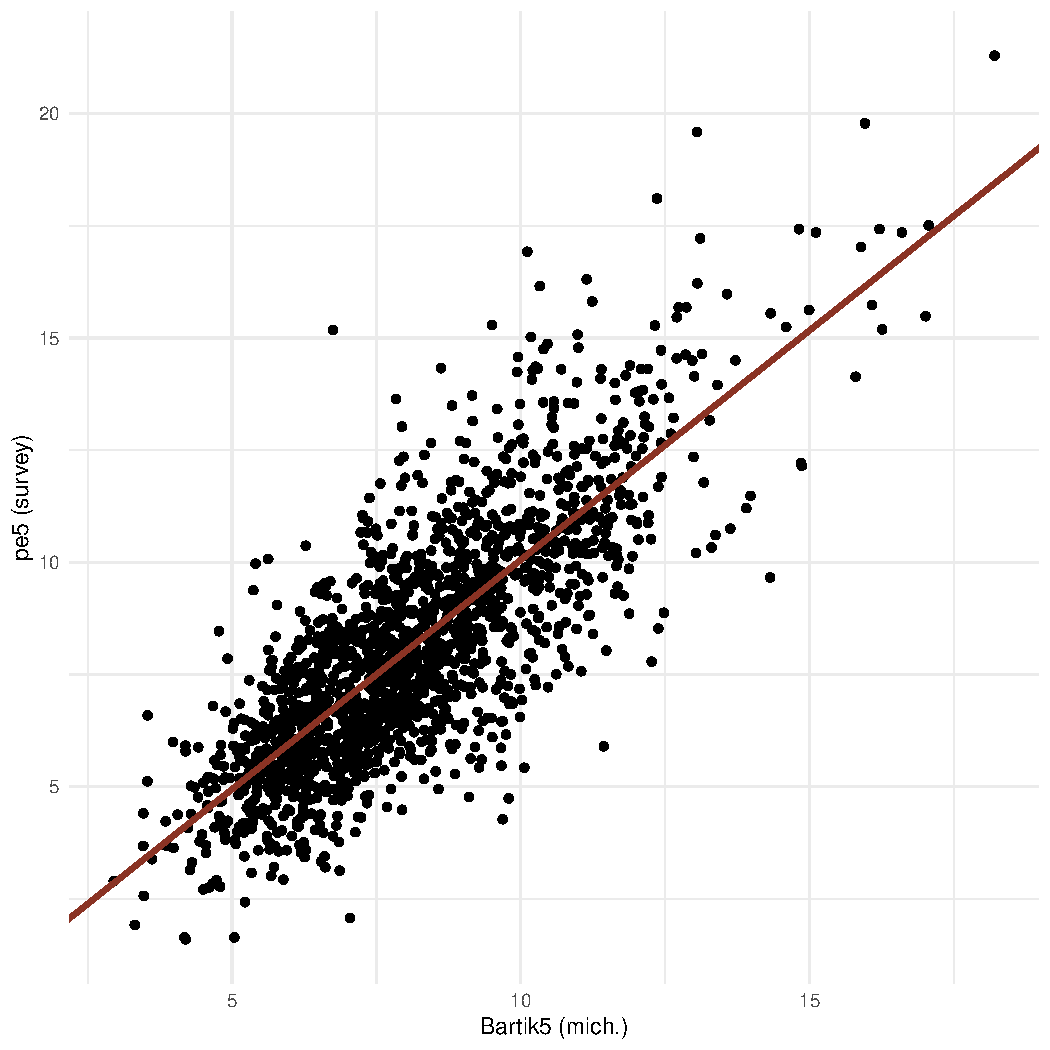
\includegraphics[width = 5in, height =3in]{figs/firstStage5only}
%\input{figs/tex/firstStage5only}
\caption{First stage long-horizon expectations only. }\label{5yearsubfig:shares:group}
\end{subfigure}
\vfill
\begin{subfigure}[t]{0.75\textwidth}
\centering
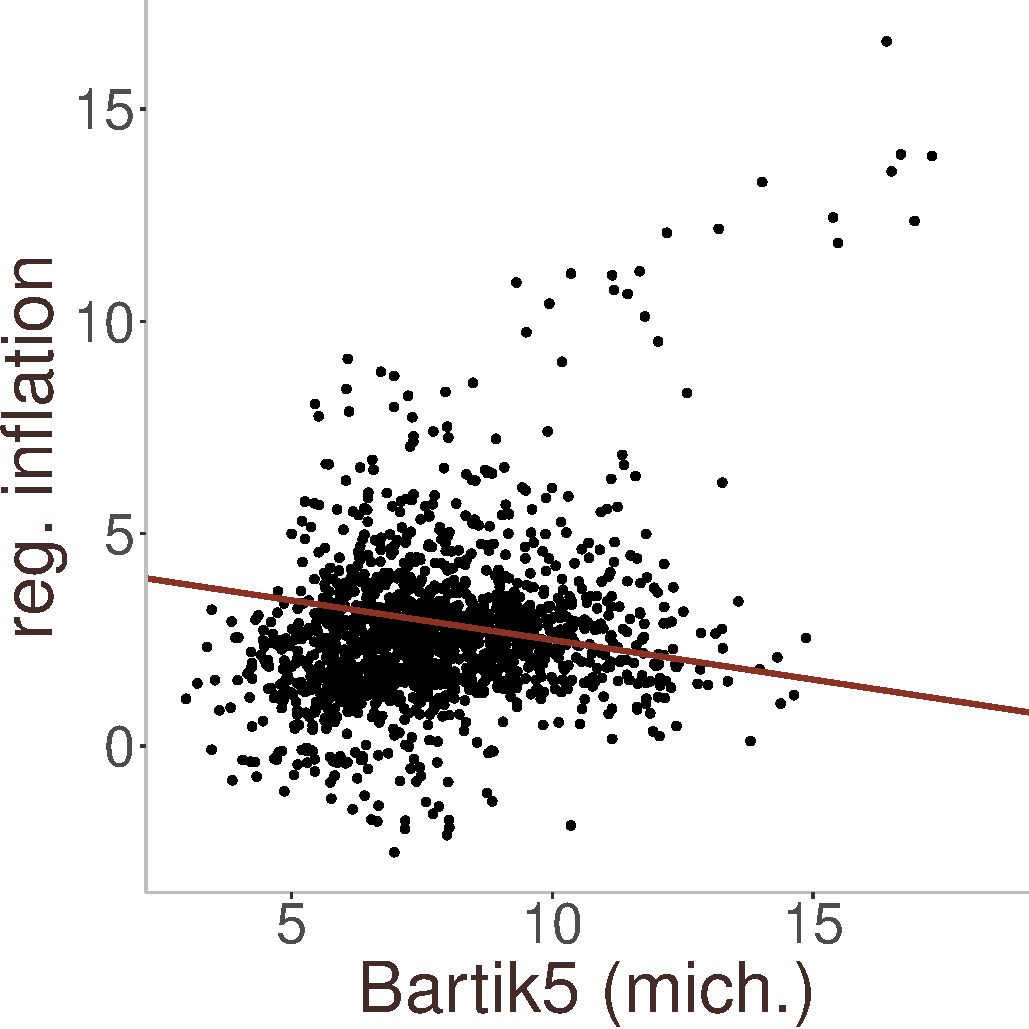
\includegraphics[width =5in, height =3in]{figs/redform5only}
%\input{figs/tex/redform5only}
\caption{Reduced form long-horizon expectations only.}\label{5yearsubfig:shares:cps}
\end{subfigure}
\end{figure}

The 2sls estimates in Tables \ref{tab:table:2sls:shortlong:stage1}-\ref{tab:table:2sls:shortlong:stage2} confirm the reduced-form findings. In the first stage, the short- and long-run instruments are relevant for both short- and long-term inflation. The long-horizon instrument has no predictive power for short-run expectations. In the second stage (Table \ref{tab:table:2sls:shortlong:stage2}), the coefficient estimates on short-run expectations are virtually identical to the preferred estimates. Long-horizon expectations have a small negative impact that is not statistically significant.  

\begin{landscape}
\begin{table}[!htbp] \centering
\caption{2SLS with short and long expectations: first stage}
\label{tab:table:2sls:shortlong:stage1}
\textbf{Panel A: CPS shares} \\ 
\begin{tabular}[t]{>{}llccccccc}
\toprule
  & (1)-pe & (1)-pe5 & (2)-pe & (2)-pe5 & (3)-pe & (3)-pe5 & (4)-pe & (4)-pe5\\
\midrule
\textbf{\cellcolor{gray!10}{Cf.}} & \cellcolor{gray!10}{0.43 (0.03)} & \cellcolor{gray!10}{-0.27 (0.1)} & \cellcolor{gray!10}{1.35 (0.09)} & \cellcolor{gray!10}{0.65 (0.11)} & \cellcolor{gray!10}{1.48 (0.03)} & \cellcolor{gray!10}{0.62 (0.11)} & \cellcolor{gray!10}{0.26 (0.13)} & \cellcolor{gray!10}{-0.24 (0.1)}\\
\textbf{$R^2$} & 0.80 & 0.40 & 0.68 & 0.18 & 0.72 & 0.19 & 0.78 & 0.38\\
\textbf{\cellcolor{gray!10}{F}} & \cellcolor{gray!10}{12.17} & \cellcolor{gray!10}{4.13} & \cellcolor{gray!10}{261.22} & \cellcolor{gray!10}{46.66} & \cellcolor{gray!10}{315.11} & \cellcolor{gray!10}{45.74} & \cellcolor{gray!10}{5.37} & \cellcolor{gray!10}{4.43}\\
\bottomrule
\end{tabular} \vspace{5mm} 
\\ \textbf{Panel B: Michigan shares} \\ 
\begin{tabular}[t]{>{}llccccccc}
\toprule
  & (1)-pe & (1)-pe5 & (2)-pe & (2)-pe5 & (3)-pe & (3)-pe5 & (4)-pe & (4)-pe5\\
\midrule
\textbf{\cellcolor{gray!10}{Cf.}} & \cellcolor{gray!10}{0.24 (0.02)} & \cellcolor{gray!10}{-0.17 (0.06)} & \cellcolor{gray!10}{0.75 (0.02)} & \cellcolor{gray!10}{0.33 (0.04)} & \cellcolor{gray!10}{0.74 (0.02)} & \cellcolor{gray!10}{0.35 (0.04)} & \cellcolor{gray!10}{0.23 (0.02)} & \cellcolor{gray!10}{-0.19 (0.05)}\\
\textbf{$R^2$} & 0.80 & 0.40 & 0.72 & 0.18 & 0.74 & 0.19 & 0.79 & 0.39\\
\textbf{\cellcolor{gray!10}{F}} & \cellcolor{gray!10}{17.17} & \cellcolor{gray!10}{6.64} & \cellcolor{gray!10}{372.11} & \cellcolor{gray!10}{42.85} & \cellcolor{gray!10}{384.19} & \cellcolor{gray!10}{45.73} & \cellcolor{gray!10}{15.48} & \cellcolor{gray!10}{8.90}\\
\bottomrule
\end{tabular}\end{table}
\end{landscape}


\begin{table}

\caption{\label{tab:2sls:shortandlong:stage2}2SLS with short and long-expectations: coefficient estimates}
\centering
\begin{threeparttable}
\begin{tabular}[t]{lll}
\toprule
  & survey & CPS78\\
\midrule
\cellcolor{gray!6}{Dependent Var.:} & \cellcolor{gray!6}{RegInf} & \cellcolor{gray!6}{RegInf}\\
\addlinespace
 &  & \\
\addlinespace
\cellcolor{gray!6}{short-run pe} & \cellcolor{gray!6}{0.3355* (0.1475)} & \cellcolor{gray!6}{0.5394** (0.1931)}\\
\addlinespace
long-run pe & -0.0228 (0.0450) & -0.0373 (0.0746)\\
\addlinespace
\cellcolor{gray!6}{Controls} & \cellcolor{gray!6}{Yes} & \cellcolor{gray!6}{Yes}\\
\addlinespace
Fixed-Effects: & ---------------- & -----------------\\
\addlinespace
\cellcolor{gray!6}{REGION} & \cellcolor{gray!6}{Yes} & \cellcolor{gray!6}{Yes}\\
\addlinespace
TIME & Yes & Yes\\
\addlinespace
\cellcolor{gray!6}{\_\_\_\_\_\_\_\_\_\_\_\_\_\_\_} & \cellcolor{gray!6}{\_\_\_\_\_\_\_\_\_\_\_\_\_\_\_\_} & \cellcolor{gray!6}{\_\_\_\_\_\_\_\_\_\_\_\_\_\_\_\_\_}\\
\addlinespace
S.E. type & Dris.-Kra. (L=4) & Drisc.-Kra. (L=4)\\
\addlinespace
\cellcolor{gray!6}{Observations} & \cellcolor{gray!6}{1,387} & \cellcolor{gray!6}{1,387}\\
\addlinespace
R2 & 0.95325 & 0.93851\\
\addlinespace
\cellcolor{gray!6}{Within R2} & \cellcolor{gray!6}{0.54716} & \cellcolor{gray!6}{0.40438}\\
\bottomrule
\end{tabular}
\begin{tablenotes}
\item \textit{Note: } 
\item Survey is the benchmark shift-share instrument using Michigan survey shares. CPS78 is constructed from the 1978.1 CPS.
\end{tablenotes}
\end{threeparttable}
\end{table}


One might wonder if long-horizon expectations proxy for short-run expectations and identify an effect acting on inflation. Tables \ref{tab:base:5only:2sls:stage1}-\ref{tab:base:5only:2sls:stage2} show that, again, there is no effect running from long-horizon expectations to inflation. While the estimated sign for long-horizon expectations is again positive, it is close to zero and insignificant.  

\begin{table}

\caption{\label{tab:2sls:long:stage1}2SLS with long-expectations: first stage}
\centering
\begin{threeparttable}
\begin{tabular}[t]{lll}
\toprule
  & survey long pe & CPS78 long pe\\
\midrule
\cellcolor{gray!6}{Dependent Var.:} & \cellcolor{gray!6}{long-run pe} & \cellcolor{gray!6}{long-run pe}\\
\addlinespace
 &  & \\
\addlinespace
\cellcolor{gray!6}{Bartik5} & \cellcolor{gray!6}{0.9923*** (0.0338)} & \cellcolor{gray!6}{0.8641*** (0.0729)}\\
\addlinespace
Controls & Yes & Yes\\
\addlinespace
\cellcolor{gray!6}{Fixed-Effects:} & \cellcolor{gray!6}{------------------} & \cellcolor{gray!6}{------------------}\\
\addlinespace
REGION & Yes & Yes\\
\addlinespace
\cellcolor{gray!6}{TIME} & \cellcolor{gray!6}{Yes} & \cellcolor{gray!6}{Yes}\\
\addlinespace
\_\_\_\_\_\_\_\_\_\_\_\_\_\_\_ & \_\_\_\_\_\_\_\_\_\_\_\_\_\_\_\_\_\_ & \_\_\_\_\_\_\_\_\_\_\_\_\_\_\_\_\_\_\\
\addlinespace
\cellcolor{gray!6}{S.E. type} & \cellcolor{gray!6}{Drisco.-Kra. (L=4)} & \cellcolor{gray!6}{Drisco.-Kra. (L=4)}\\
\addlinespace
Observations & 1,387 & 1,387\\
\addlinespace
\cellcolor{gray!6}{R2} & \cellcolor{gray!6}{0.59881} & \cellcolor{gray!6}{0.44158}\\
\addlinespace
Within R2 & 0.35600 & 0.10361\\
\bottomrule
\end{tabular}
\begin{tablenotes}
\item \textit{Note: } 
\item Survey is the benchmark shift-share instrument using Michigan survey shares. CPS78 is constructed from the 1978.1 CPS.
\end{tablenotes}
\end{threeparttable}
\end{table}

\begin{table}[!htbp] \centering
\caption{2SLS with long expectations: coefficient estimates}
\label{tab:base:5only:2sls:stage2}
\textbf{Panel A: CPS shares} \\ 
\begin{tabular}{lllll}
\toprule
 & (1) & (2) & (3) & (4)\\
\midrule
\cellcolor{gray!10}{$p5^e$} & \cellcolor{gray!10}{-0.085 (0.054)} & \cellcolor{gray!10}{0.012 (0.014)} & \cellcolor{gray!10}{0.007 (0.014)} & \cellcolor{gray!10}{-0.071 (0.077)}\\
$u^r$ & -0.145 (0.076) & 0.054 (0.029) & 0.068 (0.033) & 0.006 (0.058)\\
\hline
\cellcolor{gray!10}{N} & \cellcolor{gray!10}{1,387} & \cellcolor{gray!10}{1,387} & \cellcolor{gray!10}{1,387} & \cellcolor{gray!10}{1,387}\\
R2 & 0.947 & 0.922 & 0.921 & 0.948\\
\cellcolor{gray!10}{within R2} & \cellcolor{gray!10}{0.483} & \cellcolor{gray!10}{} & \cellcolor{gray!10}{0.92} & \cellcolor{gray!10}{0.524}\\
\addlinespace
Region FE & X &  & X & \\
\cellcolor{gray!10}{Time FE} & \cellcolor{gray!10}{X} & \cellcolor{gray!10}{} & \cellcolor{gray!10}{} & \cellcolor{gray!10}{X}\\
SE & by: REGION & by: REGION & by: REGION & by: REGION\\
\bottomrule
\end{tabular} \vspace{5mm} 
\\ \textbf{Panel B: Michigan shares} \\ 
\begin{threeparttable}
\begin{tabular}{lllll}
\toprule
 & (1) & (2) & (3) & (4)\\
\midrule
\cellcolor{gray!10}{$p5^e$} & \cellcolor{gray!10}{0.018 (0.040)} & \cellcolor{gray!10}{-0.036 (0.011)**} & \cellcolor{gray!10}{-0.035 (0.011)**} & \cellcolor{gray!10}{0.021 (0.041)}\\
$u^r$ & -0.150 (0.052)* & 0.050 (0.024) & 0.068 (0.028)* & -0.015 (0.047)\\
\hline
\cellcolor{gray!10}{N} & \cellcolor{gray!10}{1,387} & \cellcolor{gray!10}{1,387} & \cellcolor{gray!10}{1,387} & \cellcolor{gray!10}{1,387}\\
R2 & 0.96 & 0.918 & 0.917 & 0.958\\
\cellcolor{gray!10}{within R2} & \cellcolor{gray!10}{0.609} & \cellcolor{gray!10}{} & \cellcolor{gray!10}{0.916} & \cellcolor{gray!10}{0.612}\\
\addlinespace
Region FE & X &  & X & \\
\cellcolor{gray!10}{Time FE} & \cellcolor{gray!10}{X} & \cellcolor{gray!10}{} & \cellcolor{gray!10}{} & \cellcolor{gray!10}{X}\\
SE & by: REGION & by: REGION & by: REGION & by: REGION\\
\bottomrule
\end{tabular}
\begin{tablenotes}
\item \textit{Note: } 
\item Coefficient estimates with long expectations only. Instruments computed using a leave-one-out procedure. Survey is the shift-share instrument using Michigan survey shares. CPS78 is constructed from the 1978.1 CPS.
\item[1] Signif. codes: * = .1; ** = .05; *** = .01.
\end{tablenotes}
\end{threeparttable}\end{table}



The results on long-run expectations hold broader implications for monetary policy and the modeling of inflation expectations.
\section{Conclusion}


The role played by inflation expectations in the data-generating process for inflation, and other macroeconomic outcomes have been, and remains, a key question for researchers and policymakers. In part, many economic decisions by consumers and firms depend on expectations about the future path for prices and real interest rates. The quantitative impact of shocks to inflation expectations remains an open question. The standard econometric approach is to derive a New Keynesian Phillips Curve, assuming rational expectations and estimating the slope and pass-through from expectations after instrumenting for expectations. Drawbacks to the standard approach are that it requires explicit assumptions about how people form their inflation expectations and then finding a good instrument that overcomes a weak instrument problem.

This paper, instead, uses survey expectations and exploits the rich micro-data and heterogeneity in the Michigan survey to identify the impact of subjective inflation expectations on inflation outcomes. The empirical strategy begins with the observation that survey inflation expectations vary across demographic groups. The identifying assumption is that region-specific supply shocks are not disproportionately concentrated in regions with a high representation of particular demographic groups.  From this identifying assumption, a quasi-experimental differential exposure arises naturally. A shift-share instrument (``Bartik instrument'') forecasts expectations in a region as the expectations of a demographic group at the national level interacted with that group's population share in the region. The empirical strategy exploits the cross-region heterogeneity in demographic groups and the heterogeneity in expectations across groups. The shift-share instrument is plausibly exogenous as the group shares are uncorrelated with the other exogenous regressors that predict regional inflation.

The estimates identify a positive impact from inflation expectations to (regional) inflation. The identified effect is several times stronger than estimated by ordinary least squares, and the preferred estimate finds a significant positive effect. However, the pass-through from expectations to inflation is below one: a one percentage point increase in a region's inflation expectations will lead to a 60 basis point increase. The estimate does not account for cross-regional spillovers, which would likely strengthen the pass-through above one. Interestingly, one-year-ahead inflation expectations matter, and long-horizon expectations play no economically or statistically significant role. The identifying variation comes from (1.) groups of married consumers aged 18-39 with at least a high school degree and (2.) during periods of high inflation volatility such as 1978-82, 2007-2009, and the post-pandemic 2021-22.

\pagebreak

%\bibliographystyle{/Users/billbranch/Dropbox/Cloud/Research/bibliography/econometrica}
\bibliographystyle{style/econometrica}


%\bibliography{library_research_bill,harvard}

%\bibliography{/Users/billbranch/Dropbox/Cloud/Research/bibliography/library_research_bill}
\bibliography{style/library_research_bill}

\end{document}